% Options for packages loaded elsewhere
\PassOptionsToPackage{unicode}{hyperref}
\PassOptionsToPackage{hyphens}{url}
%
\documentclass[
  12pt,
]{book}
\usepackage{lmodern}
\usepackage{amssymb,amsmath}
\usepackage{ifxetex,ifluatex}
\ifnum 0\ifxetex 1\fi\ifluatex 1\fi=0 % if pdftex
  \usepackage[T1]{fontenc}
  \usepackage[utf8]{inputenc}
  \usepackage{textcomp} % provide euro and other symbols
\else % if luatex or xetex
  \usepackage{unicode-math}
  \defaultfontfeatures{Scale=MatchLowercase}
  \defaultfontfeatures[\rmfamily]{Ligatures=TeX,Scale=1}
\fi
% Use upquote if available, for straight quotes in verbatim environments
\IfFileExists{upquote.sty}{\usepackage{upquote}}{}
\IfFileExists{microtype.sty}{% use microtype if available
  \usepackage[]{microtype}
  \UseMicrotypeSet[protrusion]{basicmath} % disable protrusion for tt fonts
}{}
\makeatletter
\@ifundefined{KOMAClassName}{% if non-KOMA class
  \IfFileExists{parskip.sty}{%
    \usepackage{parskip}
  }{% else
    \setlength{\parindent}{0pt}
    \setlength{\parskip}{6pt plus 2pt minus 1pt}}
}{% if KOMA class
  \KOMAoptions{parskip=half}}
\makeatother
\usepackage{xcolor}
\IfFileExists{xurl.sty}{\usepackage{xurl}}{} % add URL line breaks if available
\IfFileExists{bookmark.sty}{\usepackage{bookmark}}{\usepackage{hyperref}}
\hypersetup{
  pdftitle={How to fit an animal model},
  pdfauthor={Julien Martin; Matthieu Videlier},
  hidelinks,
  pdfcreator={LaTeX via pandoc}}
\urlstyle{same} % disable monospaced font for URLs
\usepackage{color}
\usepackage{fancyvrb}
\newcommand{\VerbBar}{|}
\newcommand{\VERB}{\Verb[commandchars=\\\{\}]}
\DefineVerbatimEnvironment{Highlighting}{Verbatim}{commandchars=\\\{\}}
% Add ',fontsize=\small' for more characters per line
\usepackage{framed}
\definecolor{shadecolor}{RGB}{248,248,248}
\newenvironment{Shaded}{\begin{snugshade}}{\end{snugshade}}
\newcommand{\AlertTok}[1]{\textcolor[rgb]{0.94,0.16,0.16}{#1}}
\newcommand{\AnnotationTok}[1]{\textcolor[rgb]{0.56,0.35,0.01}{\textbf{\textit{#1}}}}
\newcommand{\AttributeTok}[1]{\textcolor[rgb]{0.77,0.63,0.00}{#1}}
\newcommand{\BaseNTok}[1]{\textcolor[rgb]{0.00,0.00,0.81}{#1}}
\newcommand{\BuiltInTok}[1]{#1}
\newcommand{\CharTok}[1]{\textcolor[rgb]{0.31,0.60,0.02}{#1}}
\newcommand{\CommentTok}[1]{\textcolor[rgb]{0.56,0.35,0.01}{\textit{#1}}}
\newcommand{\CommentVarTok}[1]{\textcolor[rgb]{0.56,0.35,0.01}{\textbf{\textit{#1}}}}
\newcommand{\ConstantTok}[1]{\textcolor[rgb]{0.00,0.00,0.00}{#1}}
\newcommand{\ControlFlowTok}[1]{\textcolor[rgb]{0.13,0.29,0.53}{\textbf{#1}}}
\newcommand{\DataTypeTok}[1]{\textcolor[rgb]{0.13,0.29,0.53}{#1}}
\newcommand{\DecValTok}[1]{\textcolor[rgb]{0.00,0.00,0.81}{#1}}
\newcommand{\DocumentationTok}[1]{\textcolor[rgb]{0.56,0.35,0.01}{\textbf{\textit{#1}}}}
\newcommand{\ErrorTok}[1]{\textcolor[rgb]{0.64,0.00,0.00}{\textbf{#1}}}
\newcommand{\ExtensionTok}[1]{#1}
\newcommand{\FloatTok}[1]{\textcolor[rgb]{0.00,0.00,0.81}{#1}}
\newcommand{\FunctionTok}[1]{\textcolor[rgb]{0.00,0.00,0.00}{#1}}
\newcommand{\ImportTok}[1]{#1}
\newcommand{\InformationTok}[1]{\textcolor[rgb]{0.56,0.35,0.01}{\textbf{\textit{#1}}}}
\newcommand{\KeywordTok}[1]{\textcolor[rgb]{0.13,0.29,0.53}{\textbf{#1}}}
\newcommand{\NormalTok}[1]{#1}
\newcommand{\OperatorTok}[1]{\textcolor[rgb]{0.81,0.36,0.00}{\textbf{#1}}}
\newcommand{\OtherTok}[1]{\textcolor[rgb]{0.56,0.35,0.01}{#1}}
\newcommand{\PreprocessorTok}[1]{\textcolor[rgb]{0.56,0.35,0.01}{\textit{#1}}}
\newcommand{\RegionMarkerTok}[1]{#1}
\newcommand{\SpecialCharTok}[1]{\textcolor[rgb]{0.00,0.00,0.00}{#1}}
\newcommand{\SpecialStringTok}[1]{\textcolor[rgb]{0.31,0.60,0.02}{#1}}
\newcommand{\StringTok}[1]{\textcolor[rgb]{0.31,0.60,0.02}{#1}}
\newcommand{\VariableTok}[1]{\textcolor[rgb]{0.00,0.00,0.00}{#1}}
\newcommand{\VerbatimStringTok}[1]{\textcolor[rgb]{0.31,0.60,0.02}{#1}}
\newcommand{\WarningTok}[1]{\textcolor[rgb]{0.56,0.35,0.01}{\textbf{\textit{#1}}}}
\usepackage{longtable,booktabs}
% Correct order of tables after \paragraph or \subparagraph
\usepackage{etoolbox}
\makeatletter
\patchcmd\longtable{\par}{\if@noskipsec\mbox{}\fi\par}{}{}
\makeatother
% Allow footnotes in longtable head/foot
\IfFileExists{footnotehyper.sty}{\usepackage{footnotehyper}}{\usepackage{footnote}}
\makesavenoteenv{longtable}
\usepackage{graphicx}
\makeatletter
\def\maxwidth{\ifdim\Gin@nat@width>\linewidth\linewidth\else\Gin@nat@width\fi}
\def\maxheight{\ifdim\Gin@nat@height>\textheight\textheight\else\Gin@nat@height\fi}
\makeatother
% Scale images if necessary, so that they will not overflow the page
% margins by default, and it is still possible to overwrite the defaults
% using explicit options in \includegraphics[width, height, ...]{}
\setkeys{Gin}{width=\maxwidth,height=\maxheight,keepaspectratio}
% Set default figure placement to htbp
\makeatletter
\def\fps@figure{htbp}
\makeatother
\setlength{\emergencystretch}{3em} % prevent overfull lines
\providecommand{\tightlist}{%
  \setlength{\itemsep}{0pt}\setlength{\parskip}{0pt}}
\setcounter{secnumdepth}{5}
%\usepackage{booktabs}
\usepackage{ctable}
\usepackage{fancyhdr}
\usepackage{float}
\usepackage[margin=2cm]{geometry}

\floatplacement{figure}{H}

%\usepackage[sf,bf]{titlesec}

\hypersetup{colorlinks=true, urlcolor=blue}

\renewcommand{\chaptername}{Chapitre}
\renewcommand{\contentsname}{Table des Matières}
\renewcommand{\partname}{Partie}

\usepackage{framed,color}
\definecolor{incolor}{RGB}{240,240,240}
\definecolor{outcolor}{RGB}{248,248,248}

\renewcommand{\textfraction}{0.05}
\renewcommand{\topfraction}{0.8}
\renewcommand{\bottomfraction}{0.8}
\renewcommand{\floatpagefraction}{0.75}

%\renewenvironment{quote}{\begin{VF}}{\end{VF}}

\ifxetex
 \usepackage{letltxmacro}
 \setlength{\XeTeXLinkMargin}{1pt}
 \LetLtxMacro\SavedIncludeGraphics\includegraphics
 \def\includegraphics#1#{% #1 catches optional stuff (star/opt. arg.)
   \IncludeGraphicsAux{#1}%
 }%
 \newcommand*{\IncludeGraphicsAux}[2]{%
   \XeTeXLinkBox{%
     \SavedIncludeGraphics#1{#2}%
   }%
 }%
\fi

\makeatletter
\newenvironment{kframe}{%
\medskip{}
\setlength{\fboxsep}{.8em}
\def\at@end@of@kframe{}%
\ifinner\ifhmode%
 \def\at@end@of@kframe{\end{minipage}}%
 \begin{minipage}{\columnwidth}%
\fi\fi%
\def\FrameCommand##1{\hskip\@totalleftmargin \hskip-\fboxsep
\colorbox{incolor}{##1}\hskip-\fboxsep
    % There is no \\@totalrightmargin, so:
    \hskip-\linewidth \hskip-\@totalleftmargin \hskip\columnwidth}%
\MakeFramed {\advance\hsize-\width
  \@totalleftmargin\z@ \linewidth\hsize
  \@setminipage}}%
{\par\unskip\endMakeFramed%
\at@end@of@kframe}
\makeatother

\makeatletter
\@ifundefined{Shaded}{
}{\renewenvironment{Shaded}{\begin{kframe}}{\end{kframe}}}
\makeatother

% \let\oldverbatim\verbatim
% \renewenvironment{Shaded}{\vspace{0.2cm}\begin{kframe}}{\end{kframe}}
% \renewenvironment{verbatim}{\begin{shaded}\begin{oldverbatim}}{\end{oldverbatim}\end{shaded}}

\newenvironment{rmdblock}[1]
 {
 \begin{itemize}
 \renewcommand{\labelitemi}{
   \raisebox{-.7\height}[0pt][0pt]{
     {\setkeys{Gin}{width=3em,keepaspectratio}\includegraphics{images/#1}}
   }
 }
 \begin{kframe}
 \setlength{\fboxsep}{1em}
 \item
 }
 {
 \end{kframe}
 \end{itemize}
 }
\newenvironment{rmdnote}
  {\begin{rmdblock}{note}}
  {\end{rmdblock}}
\newenvironment{rmdcaution}
  {\begin{rmdblock}{caution}}
  {\end{rmdblock}}
\newenvironment{rmdimportant}
  {\begin{rmdblock}{important}}
  {\end{rmdblock}}
\newenvironment{rmdtip}
  {\begin{rmdblock}{tip}}
  {\end{rmdblock}}
\newenvironment{rmdwarning}
  {\begin{rmdblock}{warning}}
  {\end{rmdblock}}
\newenvironment{rmdcode}
  {\begin{rmdblock}{screen}}
  {\end{rmdblock}}

\usepackage{makeidx}
\makeindex

\urlstyle{tt}

\usepackage{amsthm}
\makeatletter
\def\thm@space@setup{%
  \thm@preskip=8pt plus 2pt minus 4pt
  \thm@postskip=\thm@preskip
}
\makeatother

% \frontmatter
\usepackage[]{natbib}
\bibliographystyle{apalike}

\title{How to fit an animal model}
\usepackage{etoolbox}
\makeatletter
\providecommand{\subtitle}[1]{% add subtitle to \maketitle
  \apptocmd{\@title}{\par {\large #1 \par}}{}{}
}
\makeatother
\subtitle{An ecologist guide}
\author{Julien Martin\footnote{Univeristy of Ottawa, \href{mailto:julien.martin@uottawa.ca}{\nolinkurl{julien.martin@uottawa.ca}}} \and Matthieu Videlier\footnote{UQAM, \href{mailto:videlier.mathieu@courrier.uqam.ca}{\nolinkurl{videlier.mathieu@courrier.uqam.ca}}}}
\date{30-04-2022}

\begin{document}
\maketitle

%\cleardoublepage\newpage\thispagestyle{empty}\null
%\cleardoublepage\newpage\thispagestyle{empty}\null
%\cleardoublepage\newpage
%\thispagestyle{empty}
%\begin{center}
%
\includegraphics{images/missing.png}
%\end{center}

%\setlength{\abovedisplayskip}{-5pt}
%\setlength{\abovedisplayshortskip}{-5pt}

{
\setcounter{tocdepth}{1}
\tableofcontents
}
\hypertarget{preface}{%
\chapter*{Preface}\label{preface}}
\addcontentsline{toc}{chapter}{Preface}

This book is a collection of tutorial from the excellent paper by \citep{wilson2010}.
Instead of just copy pasting the tutorial in a bookdown format, the tutorials have been updated to work with the newest version of the softwares and extended to present other softwares.
\textbf{However, this is still a work in progress.}

\begin{rmdwarning}
Do not take anything in this manual as gospel.
\end{rmdwarning}

\hypertarget{contributors}{%
\subsection*{Contributors}\label{contributors}}
\addcontentsline{toc}{subsection}{Contributors}

List of people who contributed to update and extend tutorials:

\begin{itemize}
\tightlist
\item
  Eric Postma updated the previous tutorial from asreml-r 3 to asreml-r 4
\item
  Julien Martin developed and maintains the site
\item
  Mathieu Videlier added (and continues to add) more details in the document
\end{itemize}

\hypertarget{intro}{%
\chapter{Introduction}\label{intro}}

The book is provides a series of tutorials (and accompanying data files) to fit animal model in \texttt{R} using different packages (\texttt{ASReml-R}, \texttt{gremlin}, \texttt{MCMCglmm} and \texttt{brms}/\texttt{stan}) .
You will need to carefully follow the instructions below to first download the data files and second install the R packages.
Before beginning the tutorial, we assume the reader has successfully installed the chosen R package on their computer and has saved the required data files to an appropriate directory from which they will be read.
Full instructions for how to do this are provided with software distributions.

To work though the different tutorial I would recommend to create a folder where you will save your different \texttt{R} scripts for the tutorials.

In addition, the tutorial is here to help researchers in their coding and understanding of models and outputs, but it is required that you read and understand the literature in quantitative genetics and animal model.

\hypertarget{data}{%
\section{Data}\label{data}}

\hypertarget{data-files}{%
\subsection{Data files}\label{data-files}}

You will need to download 3 data files for the tutorial in \texttt{R}:

\begin{itemize}
\tightlist
\item
  gryphon.csv: data on gryphon birth weight and morphology
\item
  gryphonRM.csv: data on gryphon repeated measurement of lay date.
\item
  gryphonped.csv: data on the associated pedigree of the data gryphon
\end{itemize}

In addition, some models presented in the tutorials can take a while to run (sometimes \textgreater{} 1 hour), thus we are also providing the model outputs to allow you continue the tutorial without waiting for the model to run. (But you are free to run models)

The files are available \href{https://github.com/JulienGAMartin/wam_tuto/tree/master/data}{here}
I recommend to save the data and Rdata files in a subfolder \texttt{data} in the folder you will use as your working directory for R and where you will save your R scripts. It should be noted that the tutorial are using this structure to read or save data.

\hypertarget{notes-on-data-and-pedigree}{%
\subsection{Notes on data and pedigree}\label{notes-on-data-and-pedigree}}

It is always important to take time to think carefully about the strengths and potential limitations of your pedigree information before embarking on quantitative genetic analyses. Pedigree Viewer, written by Brian Kinghorn, is an extremely useful application for visualizing pedigrees, and can be downloaded from: \url{http://www-personal.une.edu.au/~bkinghor/pedigree.htm}. \texttt{Pedantics} an R package written by Michael Morrissey and distributed through CRAN (\url{http://cran.r-project.org/}) can also be used for this and offers some nice additional features for visualizing pedigree structures and generating associated statistics. Before you begin running through the tutorials, we advise taking a moment to look at the pedigree files provided with them using Pedigree Viewer or Pedantics.

\hypertarget{r}{%
\section{R}\label{r}}

You should check that you have the most current version of R and R packages. You can check the number of the current version on CRAN. If you need to update (or install) R packages, use \texttt{install.packages()} and follow the prompted instructions.

\hypertarget{r-packages}{%
\subsection{R packages}\label{r-packages}}

\hypertarget{asreml-r}{%
\subsubsection{asreml-r}\label{asreml-r}}

ASReml-R is commercial software published by VSN international (\url{http://www.vsni.co.uk/software/asreml/}). This package is not free and requires a key access.
Additional information and guide can be find in the Asreml-R manual: (\url{https://asreml.kb.vsni.co.uk/wp-content/uploads/sites/3/2018/02/ASReml-R-Reference-Manual-4.pdf})

\hypertarget{gremlin}{%
\subsubsection{gremlin}\label{gremlin}}

\texttt{gremlin} is a little monster appearing if you feed a mugwai after midnight. It is also a great and promising software written by Pr. Matthew E. Wolak to fit mixed models using a frequentist approach .

\hypertarget{mcmcglmm}{%
\subsubsection{MCMCglmm}\label{mcmcglmm}}

\texttt{MCMCglmm} is an R package for Bayesian mixed model analysis written by Pr. Jarrod Hadfield. It is a freeware distributed through CRAN (\url{http://cran.r-project.org/}). Information and guide about the package can be find in the user manual and vignettes (\url{http://cran.r-project.org/web/packages/MCMCglmm/index.html}).
Reference: \citep[\citet{R-MCMCglmm}]{MCMCglmm2010}.

This module provides some information that applies to MCMCglmm-based analyses in general, but that will not be included in other tutorials.
Most importantly, this applies to some of the simplest ways of determining the performance of a run using MCMCglmm, i.e., verification of the validity of of the posterior distribution.
This tutorial is not a substitute for working through the MCMCglmm course notes, which is available from CRAN (the Comprehensive R ArchiveNetwork, \url{http://cran.r-project.org/}, or can be accessed in R using the command vignette(``CourseNotes'',``MCMCglmm'')).
These tutorials do not introduce one of the main advantages of using MCMCglmm for analyses of data from natural populations -the ability to properly model non-normal responses.
These capabilities are introduced in the documentation that is distributed with MCMCglmm, and available from CRAN.
Another specific animal guide for MCMCglmm can be find (\url{https://devillemereuil.legtux.org/wp-content/uploads/2021/09/tuto_en.pdf}). Pr. Pierre de Villemereuil provide more information in Bayesian concept and focus more on non-gaussian variable.

\hypertarget{brms}{%
\subsubsection{brms}\label{brms}}

\texttt{brms} provides an interface to fit Bayesian generalized multivariate (non-)linear multilevel models using \texttt{Stan}, which is a C++ package for obtaining full Bayesian inference (see \url{https://mc-stan.org/}).
The formula syntax is an extended version of the syntax applied in the `lme4' package to provide a familiar and simple interface for performing regression analyses.

It should be noted that if \texttt{brms} is able to fit animal model the parametrization used is not the most efficient and can take quite longer than using a different parametrization directly in \texttt{stan}.

\hypertarget{univariate-animal-model}{%
\chapter{Univariate animal model}\label{univariate-animal-model}}

This tutorial will demonstrate how to run a univariate animal model to estimate genetic variance in birth weight in the mighty gryphons.

\hypertarget{scenario-and-data}{%
\section{Scenario and data}\label{scenario-and-data}}

\hypertarget{scenario}{%
\subsection{Scenario}\label{scenario}}

In a population of gryphons there is strong positive selection on birth weight with heavier born individuals having, on average higher fitness. To find out whether increased birth weight will evolve in response to the selection, and if so how quickly, we want to estimate the heritability of birth weight.

\hypertarget{data-files-1}{%
\subsection{Data files}\label{data-files-1}}

Open \texttt{gryphonped.csv} and \texttt{gryphon.csv} in your text editor. The structure and contents of these files is fairly self-explanatory. The pedigree file \texttt{gryphonped.csv} contains three columns containing unique IDs that correspond to each animal, its father, and its mother. Note that this is a multigenerational pedigree, with the earliest generation (for which parentage information is necessarily missing) at the beginning of the file. For later-born individuals maternal identities are all known but paternity information is incomplete (a common situation in real world applications).

The phenotype data, as well as additional factors and covariates that we may wish to include in our model are contained in \texttt{gryphon.csv}. Columns correspond to individual identity (\texttt{animal}), maternal identity (\texttt{mother}), year of birth (\texttt{byear}), sex (\texttt{sex}, where \texttt{1} is female and \texttt{2} is male), birth weight (\texttt{bwt}), and tarsus length (\texttt{tarsus}). Each row of the data file contains a record for a different offspring individual. Note that all individuals included in the data file must be included as offspring in the pedigree file.

We can read the data file, using \texttt{read.csv()} which consider by default that \texttt{NA} is the symbol for missing values and that the first line of the file contains the column headers.

It is a good idea to make sure that all variables are correctly assigned as numeric or factors:

\begin{Shaded}
\begin{Highlighting}[]
\NormalTok{gryphon}\OperatorTok{$}\NormalTok{animal \textless{}{-}}\StringTok{ }\KeywordTok{as.factor}\NormalTok{(gryphon}\OperatorTok{$}\NormalTok{animal)}
\NormalTok{gryphon}\OperatorTok{$}\NormalTok{mother \textless{}{-}}\StringTok{ }\KeywordTok{as.factor}\NormalTok{(gryphon}\OperatorTok{$}\NormalTok{mother)}
\NormalTok{gryphon}\OperatorTok{$}\NormalTok{byear \textless{}{-}}\StringTok{ }\KeywordTok{as.factor}\NormalTok{(gryphon}\OperatorTok{$}\NormalTok{byear)}
\NormalTok{gryphon}\OperatorTok{$}\NormalTok{sex \textless{}{-}}\StringTok{ }\KeywordTok{as.factor}\NormalTok{(gryphon}\OperatorTok{$}\NormalTok{sex)}
\NormalTok{gryphon}\OperatorTok{$}\NormalTok{bwt \textless{}{-}}\StringTok{ }\KeywordTok{as.numeric}\NormalTok{(gryphon}\OperatorTok{$}\NormalTok{bwt)}
\NormalTok{gryphon}\OperatorTok{$}\NormalTok{tarsus \textless{}{-}}\StringTok{ }\KeywordTok{as.numeric}\NormalTok{(gryphon}\OperatorTok{$}\NormalTok{tarsus)}
\KeywordTok{str}\NormalTok{(gryphon)}
\end{Highlighting}
\end{Shaded}

\begin{verbatim}
## 'data.frame':    1084 obs. of  6 variables:
##  $ animal: Factor w/ 1084 levels "1","2","3","5",..: 864 1076 549 989 1030 751 987 490 906 591 ...
##  $ mother: Factor w/ 429 levels "1","2","3","8",..: 362 268 216 375 396 289 328 255 347 240 ...
##  $ byear : Factor w/ 34 levels "968","970","971",..: 1 1 2 2 2 2 3 3 3 3 ...
##  $ sex   : Factor w/ 2 levels "1","2": 1 1 2 1 2 1 2 1 1 1 ...
##  $ bwt   : num  10.77 9.3 3.98 5.39 12.12 ...
##  $ tarsus: num  24.8 22.5 12.9 20.5 NA ...
\end{verbatim}

Similarly we can read in the pedigree file, using \texttt{read.csv()} which consider by default that \texttt{NA} is the symbol for missing values and that the first line of the file contains the column headers.

\begin{verbatim}
## 'data.frame':    1309 obs. of  3 variables:
##  $ id    : int  1306 1304 1298 1293 1290 1288 1284 1283 1282 1278 ...
##  $ father: int  NA NA NA NA NA NA NA NA NA NA ...
##  $ mother: int  NA NA NA NA NA NA NA NA NA NA ...
\end{verbatim}

\begin{Shaded}
\begin{Highlighting}[]
\NormalTok{gryphonped}\OperatorTok{$}\NormalTok{id \textless{}{-}}\StringTok{ }\KeywordTok{as.factor}\NormalTok{(gryphonped}\OperatorTok{$}\NormalTok{id)}
\NormalTok{gryphonped}\OperatorTok{$}\NormalTok{father \textless{}{-}}\StringTok{ }\KeywordTok{as.factor}\NormalTok{(gryphonped}\OperatorTok{$}\NormalTok{father)}
\NormalTok{gryphonped}\OperatorTok{$}\NormalTok{mother \textless{}{-}}\StringTok{ }\KeywordTok{as.factor}\NormalTok{(gryphonped}\OperatorTok{$}\NormalTok{mother)}
\KeywordTok{str}\NormalTok{(gryphonped)}
\end{Highlighting}
\end{Shaded}

\begin{verbatim}
## 'data.frame':    1309 obs. of  3 variables:
##  $ id    : Factor w/ 1309 levels "1","2","3","4",..: 1306 1304 1298 1293 1290 1288 1284 1283 1282 1278 ...
##  $ father: Factor w/ 158 levels "4","13","18",..: NA NA NA NA NA NA NA NA NA NA ...
##  $ mother: Factor w/ 429 levels "1","2","3","8",..: NA NA NA NA NA NA NA NA NA NA ...
\end{verbatim}

Now that we have imported the data and the pedigree file, we are ready to fit an animal model.

\hypertarget{asreml-r-1}{%
\section{Asreml-R}\label{asreml-r-1}}

\hypertarget{running-the-model}{%
\subsection{Running the model}\label{running-the-model}}

First we need to load the \texttt{asreml} library:

\begin{Shaded}
\begin{Highlighting}[]
\KeywordTok{library}\NormalTok{(asreml)}
\end{Highlighting}
\end{Shaded}

To be able to fit an animal model, Asreml-r needs (the inverse of) the relationship matrix using the ainverse function:

\begin{Shaded}
\begin{Highlighting}[]
\NormalTok{ainv \textless{}{-}}\StringTok{ }\KeywordTok{ainverse}\NormalTok{(gryphonped)}
\end{Highlighting}
\end{Shaded}

We are now ready to specify our first model:

\begin{Shaded}
\begin{Highlighting}[]
\NormalTok{model1 \textless{}{-}}\StringTok{ }\KeywordTok{asreml}\NormalTok{(}
  \DataTypeTok{fixed =}\NormalTok{ bwt }\OperatorTok{\textasciitilde{}}\StringTok{ }\DecValTok{1}\NormalTok{, }\DataTypeTok{random =} \OperatorTok{\textasciitilde{}}\StringTok{ }\KeywordTok{vm}\NormalTok{(animal, ainv),}
  \DataTypeTok{residual =} \OperatorTok{\textasciitilde{}}\StringTok{ }\KeywordTok{idv}\NormalTok{(units),}
  \DataTypeTok{data =}\NormalTok{ gryphon,}
  \DataTypeTok{na.action =} \KeywordTok{na.method}\NormalTok{(}\DataTypeTok{x =} \StringTok{"omit"}\NormalTok{, }\DataTypeTok{y =} \StringTok{"omit"}\NormalTok{)}
\NormalTok{)}
\end{Highlighting}
\end{Shaded}

\begin{verbatim}
## Online License checked out Sat Apr 30 11:04:15 2022
## Model fitted using the sigma parameterization.
## ASReml 4.1.0 Sat Apr 30 11:04:15 2022
##           LogLik        Sigma2     DF     wall    cpu
##  1     -4128.454           1.0    853 11:04:15    0.0
##  2     -3284.272           1.0    853 11:04:15    0.0
##  3     -2354.992           1.0    853 11:04:15    0.0
##  4     -1710.357           1.0    853 11:04:15    0.0
##  5     -1363.555           1.0    853 11:04:15    0.0
##  6     -1263.516           1.0    853 11:04:15    0.0
##  7     -1247.854           1.0    853 11:04:15    0.0
##  8     -1247.185           1.0    853 11:04:15    0.0
##  9     -1247.183           1.0    853 11:04:15    0.0
\end{verbatim}

In this model, \texttt{bwt} is the response variable and the only fixed effect is the intercept, denoted as \texttt{1}. The only random effect we have fitted is \texttt{animal}, which will provide an estimate of \(V_A\). Our random \texttt{animal} effect is connected to the inverse related matrix \texttt{ainv} which integrate the relativeness or pedigree information.\\
\texttt{data=} specifies the name of the dataframe that contains our variables. Finally, we inform \texttt{asreml()} what to when it encounters \texttt{NA}s in either the dependent or predictor variables (in this case we choose to remove the records).
If you use the argument ``include'' instead of ``omit'', model will keep the NA. With x=``include'', the model will exchange \texttt{NA} with 0. Be careful you need to standardize your trait so the mean will be equal to 0, if not estimates (including covariance in multivariate models) could be strongly biased due to the the missing values considered as 0. y=``include'' will exchange \texttt{NA} with a factor labeled \texttt{mv} which will be included in the sparse equation. For more details see Asreml-R manual.

A note of the specification of the structure of the residuals: This simple univariate model will run fine without \texttt{residual=\textasciitilde{}idv(units)}. However, if you are going to use \texttt{vpredict()} to calculate the heritability (see below), without specifying the residuals in this way will result in a standard error for the heritability that is incorrect.

Any model has assumption which need to be checked. The model can be plot which help visualizing the distribution of the model residual and check the different assumptions.

\begin{Shaded}
\begin{Highlighting}[]
\KeywordTok{plot}\NormalTok{(model1)}
\end{Highlighting}
\end{Shaded}

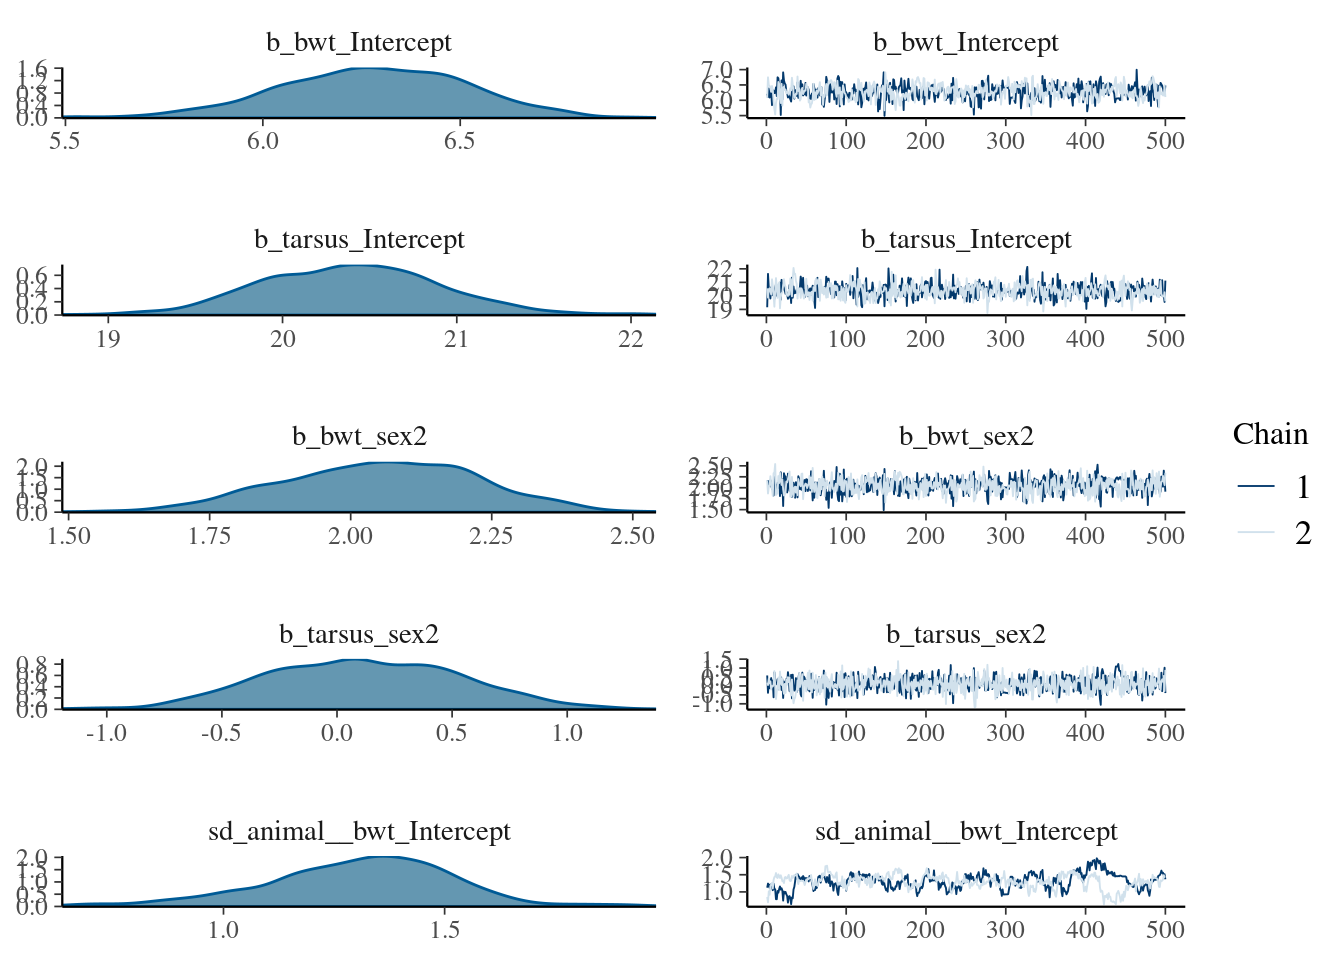
\includegraphics{wam_tuto_files/figure-latex/unnamed-chunk-10-1.pdf}

To see the estimates for the variance components, we run:

\begin{Shaded}
\begin{Highlighting}[]
\KeywordTok{summary}\NormalTok{(model1)}\OperatorTok{$}\NormalTok{varcomp}
\end{Highlighting}
\end{Shaded}

\begin{verbatim}
##                  component std.error  z.ratio bound %ch
## vm(animal, ainv)  3.395398 0.6349915 5.347154     P   0
## units!units       3.828602 0.5185919 7.382687     P   0
## units!R           1.000000        NA       NA     F   0
\end{verbatim}

We fitted a single random effect so we partitioned the phenotypic variance into two components. The \texttt{vm(animal,\ ainv)} variance component is \(V_A\) and is estimated as 3.4. Given that the ratio of \(V_A\) to its standard error (\texttt{z.ratio}) is considerably larger than 2 (\emph{i.e.} the parameter estimate is more than 2 SEs from zero), this looks likely to be significant. The \texttt{units!units} component refers to the residual variance \(V_R\), and \texttt{units\$R} should be ignored. If you don't include \texttt{residual=\textasciitilde{}idv(units)}in your model specification, \texttt{units\$R} will provide you with the residual variance.

\hypertarget{estimating-heritability}{%
\subsection{Estimating heritability}\label{estimating-heritability}}

We can calculate the \(h^2\) of birth weight from the components above since \(h^2 = V_A/V_P = V_A/(V_A+V_R)\). Thus according to this model, \(h^2\) = 3.4 / (3.4 + 3.83) = 0.47.

Alternatively we can use the \texttt{vpredict()} function to calculate \(h^2\) and its standard error. \texttt{vpredict()}function has two structures, first the model used (here \texttt{model1}) and then the estimate name with its associated equation. The equation used different \texttt{V} and their associated numbers depend of the order of the different random and residual effects included in the model.

\begin{Shaded}
\begin{Highlighting}[]
\KeywordTok{vpredict}\NormalTok{(model1, h2.bwt }\OperatorTok{\textasciitilde{}}\StringTok{ }\NormalTok{V1 }\OperatorTok{/}\StringTok{ }\NormalTok{(V1 }\OperatorTok{+}\StringTok{ }\NormalTok{V2))}
\end{Highlighting}
\end{Shaded}

\begin{verbatim}
##         Estimate         SE
## h2.bwt 0.4700163 0.07650881
\end{verbatim}

\hypertarget{adding-fixed-effects}{%
\subsection{Adding fixed effects}\label{adding-fixed-effects}}

To add fixed effects to a univariate model, we simply modify the model statement. For example, we might know (or suspect) that birth weight is a sexually dimorphic trait and therefore fit in the model.

\begin{Shaded}
\begin{Highlighting}[]
\NormalTok{model2 \textless{}{-}}\StringTok{ }\KeywordTok{asreml}\NormalTok{(}
  \DataTypeTok{fixed =}\NormalTok{ bwt }\OperatorTok{\textasciitilde{}}\StringTok{ }\DecValTok{1} \OperatorTok{+}\StringTok{ }\NormalTok{sex,}
  \DataTypeTok{random =} \OperatorTok{\textasciitilde{}}\StringTok{ }\KeywordTok{vm}\NormalTok{(animal, ainv),}
  \DataTypeTok{residual =} \OperatorTok{\textasciitilde{}}\StringTok{ }\KeywordTok{idv}\NormalTok{(units),}
  \DataTypeTok{data =}\NormalTok{ gryphon,}
  \DataTypeTok{na.action =} \KeywordTok{na.method}\NormalTok{(}\DataTypeTok{x =} \StringTok{"omit"}\NormalTok{, }\DataTypeTok{y =} \StringTok{"omit"}\NormalTok{)}
\NormalTok{)}
\end{Highlighting}
\end{Shaded}

\begin{verbatim}
## Model fitted using the sigma parameterization.
## ASReml 4.1.0 Sat Apr 30 11:04:16 2022
##           LogLik        Sigma2     DF     wall    cpu
##  1     -3364.126           1.0    852 11:04:16    0.0
##  2     -2702.117           1.0    852 11:04:16    0.0
##  3     -1978.916           1.0    852 11:04:16    0.0
##  4     -1487.834           1.0    852 11:04:16    0.0
##  5     -1236.350           1.0    852 11:04:16    0.0
##  6     -1172.771           1.0    852 11:04:16    0.0
##  7     -1165.270           1.0    852 11:04:16    0.0
##  8     -1165.093           1.0    852 11:04:16    0.0
##  9     -1165.093           1.0    852 11:04:16    0.0
\end{verbatim}

Now we can look at the fixed effects parameters and assess their significance with a conditional Wald F-test:

\begin{Shaded}
\begin{Highlighting}[]
\KeywordTok{summary}\NormalTok{(model2, }\DataTypeTok{coef =} \OtherTok{TRUE}\NormalTok{)}\OperatorTok{$}\NormalTok{coef.fixed}
\KeywordTok{wald.asreml}\NormalTok{(model2, }\DataTypeTok{ssType =} \StringTok{"conditional"}\NormalTok{, }\DataTypeTok{denDF =} \StringTok{"numeric"}\NormalTok{)}
\end{Highlighting}
\end{Shaded}

\begin{verbatim}
##             solution std error  z.ratio
## sex_1       0.000000        NA       NA
## sex_2       2.206996 0.1619974 13.62365
## (Intercept) 6.058669 0.1718244 35.26082
\end{verbatim}

\begin{verbatim}
## Model fitted using the sigma parameterization.
\end{verbatim}

\begin{verbatim}
## Warning in asreml(fixed = bwt ~ 1 + sex, random = ~vm(animal, ainv), residual =
## ~idv(units), : Algebraic derivatives for denominator df not available.
\end{verbatim}

\begin{verbatim}
## ASReml 4.1.0 Sat Apr 30 11:04:16 2022
##           LogLik        Sigma2     DF     wall    cpu
##  1     -1165.093           1.0    852 11:04:16    0.0
##  2     -1165.093           1.0    852 11:04:16    0.0
## Calculating denominator DF
\end{verbatim}

\begin{verbatim}
## $Wald
## 
##             Df denDF  F.inc  F.con Margin          Pr
## (Intercept)  1   251 3491.0 3491.0        0.00000e+00
## sex          1   831  185.6  185.6      A 2.70204e-38
## 
## $stratumVariances
##                         df Variance vm(animal, ainv) units!units
## vm(animal, ainv) 752.28476 5.957254        0.9864077           1
## units!units       99.71524 2.938413        0.0000000           1
\end{verbatim}

The very small probability (\texttt{Pr}) in the Wald test above shows that \texttt{sex} is a highly significant fixed effect, and from the parameter estimates (\texttt{summary(model2,coef=T)\$coef.fixed}) we can see that the average male (sex 2) is 2.2 kg (\(\pm\) 0.16 SE) heavier than the average female (sex 1). However, when we look at the variance components in the model including \texttt{sex} as a fixed effect, we see that they have changed slightly from the previous model:

\begin{Shaded}
\begin{Highlighting}[]
\KeywordTok{summary}\NormalTok{(model2)}\OperatorTok{$}\NormalTok{varcomp}
\end{Highlighting}
\end{Shaded}

\begin{verbatim}
##                  component std.error  z.ratio bound %ch
## vm(animal, ainv)  3.060441 0.5243571 5.836558     P   0
## units!units       2.938412 0.4161473 7.060991     P   0
## units!R           1.000000        NA       NA     F   0
\end{verbatim}

In fact since \texttt{sex} effects were previously contributing to the residual variance of the model, our estimate of \(V_R\) (denoted \texttt{units!R} in the output) is now slightly lower than before. This has an important consequence for estimating heritability since if we calculate \(V_P\) as \(V_A\)+\(V_R\) then as we include fixed effects we will soak up more residual variance driving \(V_P\). Assuming that \(V_A\) is more or less unaffected by the fixed effects fitted then as \(V_P\) goes down we expect our estimate of \(h^2\) will go up:

\begin{Shaded}
\begin{Highlighting}[]
\NormalTok{(h2}\FloatTok{.1}\NormalTok{ \textless{}{-}}\StringTok{ }\KeywordTok{vpredict}\NormalTok{(model1, h2.bwt }\OperatorTok{\textasciitilde{}}\StringTok{ }\NormalTok{V1 }\OperatorTok{/}\StringTok{ }\NormalTok{(V1 }\OperatorTok{+}\StringTok{ }\NormalTok{V2)))}
\end{Highlighting}
\end{Shaded}

\begin{verbatim}
##         Estimate         SE
## h2.bwt 0.4700163 0.07650881
\end{verbatim}

\begin{Shaded}
\begin{Highlighting}[]
\NormalTok{(h2}\FloatTok{.2}\NormalTok{ \textless{}{-}}\StringTok{ }\KeywordTok{vpredict}\NormalTok{(model2, h2.bwt }\OperatorTok{\textasciitilde{}}\StringTok{ }\NormalTok{V1 }\OperatorTok{/}\StringTok{ }\NormalTok{(V1 }\OperatorTok{+}\StringTok{ }\NormalTok{V2)))}
\end{Highlighting}
\end{Shaded}

\begin{verbatim}
##        Estimate         SE
## h2.bwt 0.510171 0.07432388
\end{verbatim}

Here \(h^2\) has increased slightly from 0.47 to 0.51. Which is the better estimate? It depends on what your question is. The first is an estimate of the proportion of variance in birth weight explained by additive effects, the latter is an estimate of the proportion of variance in birth weight \emph{after conditioning on sex} that is explained by additive effects.

An important piece of advice, each researcher should be consistent in how they name their estimates and always correctly describe which estimates they are using conditional or not (to avoid any confusion).

\hypertarget{adding-random-effects}{%
\subsection{Adding random effects}\label{adding-random-effects}}

This is done by simply modifying the model statement in the same way. For instance fitting:

\begin{Shaded}
\begin{Highlighting}[]
\NormalTok{model3 \textless{}{-}}\StringTok{ }\KeywordTok{asreml}\NormalTok{(}
  \DataTypeTok{fixed =}\NormalTok{ bwt }\OperatorTok{\textasciitilde{}}\StringTok{ }\DecValTok{1} \OperatorTok{+}\StringTok{ }\NormalTok{sex,}
  \DataTypeTok{random =} \OperatorTok{\textasciitilde{}}\StringTok{ }\KeywordTok{vm}\NormalTok{(animal, ainv) }\OperatorTok{+}\StringTok{ }\NormalTok{byear,}
  \DataTypeTok{residual =} \OperatorTok{\textasciitilde{}}\StringTok{ }\KeywordTok{idv}\NormalTok{(units),}
  \DataTypeTok{data =}\NormalTok{ gryphon,}
  \DataTypeTok{na.action =} \KeywordTok{na.method}\NormalTok{(}\DataTypeTok{x =} \StringTok{"omit"}\NormalTok{, }\DataTypeTok{y =} \StringTok{"omit"}\NormalTok{)}
\NormalTok{)}
\end{Highlighting}
\end{Shaded}

\begin{verbatim}
## Model fitted using the sigma parameterization.
## ASReml 4.1.0 Sat Apr 30 11:04:16 2022
##           LogLik        Sigma2     DF     wall    cpu
##  1     -2742.658           1.0    852 11:04:16    0.0
##  2     -2237.268           1.0    852 11:04:16    0.0
##  3     -1690.453           1.0    852 11:04:16    0.0
##  4     -1328.910           1.0    852 11:04:16    0.0
##  5     -1154.597           1.0    852 11:04:16    0.0
##  6     -1116.992           1.0    852 11:04:16    0.0
##  7     -1113.809           1.0    852 11:04:16    0.0
##  8     -1113.772           1.0    852 11:04:16    0.0
##  9     -1113.772           1.0    852 11:04:16    0.0
\end{verbatim}

\begin{Shaded}
\begin{Highlighting}[]
\KeywordTok{summary}\NormalTok{(model3)}\OperatorTok{$}\NormalTok{varcomp}
\end{Highlighting}
\end{Shaded}

\begin{verbatim}
##                  component std.error  z.ratio bound %ch
## byear            0.8862604 0.2695918 3.287416     P   0
## vm(animal, ainv) 2.7068665 0.4422140 6.121169     P   0
## units!units      2.3092415 0.3451025 6.691466     P   0
## units!R          1.0000000        NA       NA     F   0
\end{verbatim}

\begin{Shaded}
\begin{Highlighting}[]
\NormalTok{(h2}\FloatTok{.3}\NormalTok{ \textless{}{-}}\StringTok{ }\KeywordTok{vpredict}\NormalTok{(model3, h2.bwt }\OperatorTok{\textasciitilde{}}\StringTok{ }\NormalTok{V2 }\OperatorTok{/}\StringTok{ }\NormalTok{(V1 }\OperatorTok{+}\StringTok{ }\NormalTok{V2 }\OperatorTok{+}\StringTok{ }\NormalTok{V3)))}
\end{Highlighting}
\end{Shaded}

\begin{verbatim}
##         Estimate         SE
## h2.bwt 0.4586068 0.06740364
\end{verbatim}

Here the variance in \texttt{bwt} explained by \texttt{byear} is 0.89 and, based on the \texttt{z.ratio}, appears to be significant (\textgreater2). Thus we would conclude that year-to-year variation (\emph{e.g.}, in weather, resource abundance) contributes to \(V_P\). Note that although \(V_A\) has changed somewhat, as most of what is now partitioned as a birth year effect was previously partitioned as \(V_R\). Thus what we have really done here is to partition environmental effects into those arising from year-to-year differences versus everything else, and we do not really expect much change in \(h^2\) (since now \(h^2 = V_A/ (V_A+V_{BY}+V_R)\)).

However, we get a somewhat different result if we also add a random effect of \texttt{mother} to test for maternal effects:

\begin{Shaded}
\begin{Highlighting}[]
\NormalTok{model4 \textless{}{-}}\StringTok{ }\KeywordTok{asreml}\NormalTok{(}
  \DataTypeTok{fixed =}\NormalTok{ bwt }\OperatorTok{\textasciitilde{}}\StringTok{ }\DecValTok{1} \OperatorTok{+}\StringTok{ }\NormalTok{sex,}
  \DataTypeTok{random =} \OperatorTok{\textasciitilde{}}\StringTok{ }\KeywordTok{vm}\NormalTok{(animal, ainv) }\OperatorTok{+}\StringTok{ }\NormalTok{byear }\OperatorTok{+}\StringTok{ }\NormalTok{mother,}
  \DataTypeTok{residual =} \OperatorTok{\textasciitilde{}}\StringTok{ }\KeywordTok{idv}\NormalTok{(units),}
  \DataTypeTok{data =}\NormalTok{ gryphon,}
  \DataTypeTok{na.action =} \KeywordTok{na.method}\NormalTok{(}\DataTypeTok{x =} \StringTok{"omit"}\NormalTok{, }\DataTypeTok{y =} \StringTok{"omit"}\NormalTok{)}
\NormalTok{)}
\end{Highlighting}
\end{Shaded}

\begin{verbatim}
## Model fitted using the sigma parameterization.
## ASReml 4.1.0 Sat Apr 30 11:04:16 2022
##           LogLik        Sigma2     DF     wall    cpu
##  1     -2033.178           1.0    852 11:04:16    0.0
##  2     -1723.734           1.0    852 11:04:16    0.0
##  3     -1396.354           1.0    852 11:04:16    0.0
##  4     -1193.012           1.0    852 11:04:16    0.0
##  5     -1107.946           1.0    852 11:04:16    0.0
##  6     -1095.327           1.0    852 11:04:16    0.0
##  7     -1094.816           1.0    852 11:04:16    0.0
##  8     -1094.815           1.0    852 11:04:16    0.0
\end{verbatim}

\begin{Shaded}
\begin{Highlighting}[]
\KeywordTok{summary}\NormalTok{(model4)}\OperatorTok{$}\NormalTok{varcomp}
\end{Highlighting}
\end{Shaded}

\begin{verbatim}
##                  component std.error  z.ratio bound %ch
## byear            0.8820313 0.2632455 3.350604     P   0
## mother           1.1184698 0.2386239 4.687167     P   0
## vm(animal, ainv) 2.2985320 0.4962496 4.631806     P   0
## units!units      1.6290034 0.3714154 4.385934     P   0
## units!R          1.0000000        NA       NA     F   0
\end{verbatim}

\begin{Shaded}
\begin{Highlighting}[]
\NormalTok{(h2}\FloatTok{.4}\NormalTok{ \textless{}{-}}\StringTok{ }\KeywordTok{vpredict}\NormalTok{(model4, h2.bwt }\OperatorTok{\textasciitilde{}}\StringTok{ }\NormalTok{V1 }\OperatorTok{/}\StringTok{ }\NormalTok{(V1 }\OperatorTok{+}\StringTok{ }\NormalTok{V2 }\OperatorTok{+}\StringTok{ }\NormalTok{V3 }\OperatorTok{+}\StringTok{ }\NormalTok{V4)))}
\end{Highlighting}
\end{Shaded}

\begin{verbatim}
##         Estimate         SE
## h2.bwt 0.1487898 0.03861552
\end{verbatim}

Here partitioning of significant maternal variance has resulted in a further decrease in \(V_R\) but also a decrease in \(V_A\). The latter is because maternal effects of the sort we simulated (fixed differences between mothers) will have the consequence of increasing similarity among maternal siblings. Consequently they can look very much like additive genetic effects and if present, but unmodelled, represent a type of ``common environment effect'' that can - and will - cause upward bias in \(V_A\) and so \(h^2\).
The ``common environment'' can be conceived as the inextricable sum of the maternal additive genetic effect (such as maternal loci) and the maternal environment or permanent environment (such as litter or nest environment created or modified by the mother).

\hypertarget{testing-significance-of-random-effects}{%
\subsection{Testing significance of random effects}\label{testing-significance-of-random-effects}}

An important point to note in this tutorial is that while the \texttt{z.ratio} (\texttt{component}/\texttt{std.error}) reported is a good indicator of likely statistical significance (\textgreater1.96?), the standard errors are approximate and are not recommended for formal hypothesis testing. A better approach is to use likelihood-ratio tests (LRT).

For example, to test the significance of maternal effects we could compare models with and without the inclusion of maternal identity as a random effect and compare the final log-likelihoods of these models.

\begin{Shaded}
\begin{Highlighting}[]
\NormalTok{model4}\OperatorTok{$}\NormalTok{loglik}
\end{Highlighting}
\end{Shaded}

\begin{verbatim}
## [1] -1094.815
\end{verbatim}

shows that the model including maternal identity has a log-likelihood of -1094.815, and

\begin{Shaded}
\begin{Highlighting}[]
\NormalTok{model3}\OperatorTok{$}\NormalTok{loglik}
\end{Highlighting}
\end{Shaded}

\begin{verbatim}
## [1] -1113.772
\end{verbatim}

shows that the model excluding maternal identity has a log-likelihood of -1113.772.

A test statistic equal to twice the absolute difference in these log-likelihoods is assumed to be distributed as Chi square with \texttt{one} degree of freedom (one term of difference between the two models). In this case we would conclude that the maternal effects are highly significant since:
2 \(\times\) (-1094.8145793 - -1113.7719147) equals 37.9146708, and the p-value that comes with this is:

\begin{Shaded}
\begin{Highlighting}[]
\DecValTok{1} \OperatorTok{{-}}\StringTok{ }\KeywordTok{pchisq}\NormalTok{(}\DecValTok{2} \OperatorTok{*}\StringTok{ }\NormalTok{(model4}\OperatorTok{$}\NormalTok{loglik }\OperatorTok{{-}}\StringTok{ }\NormalTok{model3}\OperatorTok{$}\NormalTok{loglik), }\DecValTok{1}\NormalTok{)}
\end{Highlighting}
\end{Shaded}

\begin{verbatim}
## [1] 7.390738e-10
\end{verbatim}

As P \textless{} 0.0001 we would therefore conclude that the additional of maternal identity as a random effect significantly improves the fit of the model, given an increase in log-likelihood of approximately 19.

\hypertarget{further-partitioning-the-variance}{%
\subsection{Further partitioning the variance}\label{further-partitioning-the-variance}}

A population can be further fragmented into different groups or categories (such as females and males, juveniles and adults or treated and untreated). Some scientific questions require further and deeper analysis of the variance.
To avoid multiple model (one for each group), we can directly partition the variance between groups in a unique model. In addition, by doing so, we can also test if the variance are different between groups.

As example, we decide to take the model4 and partition its additive genetic variance and residual variance by sex. It is possible to further partition the other random effects but it will complexity the animal model and requires sufficient sample size.

First, it required to order the dataset by group (here sex).

\begin{Shaded}
\begin{Highlighting}[]
\NormalTok{gryphon \textless{}{-}}\StringTok{ }\NormalTok{gryphon[}\KeywordTok{order}\NormalTok{(gryphon}\OperatorTok{$}\NormalTok{sex), ]}
\end{Highlighting}
\end{Shaded}

To partition variances between sex, two distinct functions are require \texttt{at()} for the random level, and \texttt{dsum()} for the residual level:

\begin{Shaded}
\begin{Highlighting}[]
\NormalTok{model\_SEX \textless{}{-}}\StringTok{ }\KeywordTok{asreml}\NormalTok{(}
  \DataTypeTok{fixed =}\NormalTok{ bwt }\OperatorTok{\textasciitilde{}}\StringTok{ }\DecValTok{1} \OperatorTok{+}\StringTok{ }\NormalTok{sex,}
  \DataTypeTok{random =} \OperatorTok{\textasciitilde{}}\StringTok{ }\KeywordTok{at}\NormalTok{(sex)}\OperatorTok{:}\KeywordTok{vm}\NormalTok{(animal, ainv) }\OperatorTok{+}\StringTok{ }\NormalTok{byear }\OperatorTok{+}\StringTok{ }\NormalTok{mother,}
  \DataTypeTok{residual =} \OperatorTok{\textasciitilde{}}\StringTok{ }\KeywordTok{dsum}\NormalTok{(}\OperatorTok{\textasciitilde{}}\StringTok{ }\NormalTok{units }\OperatorTok{|}\StringTok{ }\NormalTok{sex),}
  \DataTypeTok{data =}\NormalTok{ gryphon,}
  \DataTypeTok{na.action =} \KeywordTok{na.method}\NormalTok{(}\DataTypeTok{x =} \StringTok{"omit"}\NormalTok{, }\DataTypeTok{y =} \StringTok{"omit"}\NormalTok{)}
\NormalTok{)}
\end{Highlighting}
\end{Shaded}

\begin{verbatim}
## Multi-section model using the sigma parameterization.
## ASReml 4.1.0 Sat Apr 30 11:04:17 2022
##           LogLik        Sigma2     DF     wall    cpu
##  1     -1142.164           1.0    852 11:04:17    0.0
##  2     -1126.308           1.0    852 11:04:17    0.0
##  3     -1111.536           1.0    852 11:04:17    0.0
##  4     -1105.383           1.0    852 11:04:17    0.0
##  5     -1104.375           1.0    852 11:04:17    0.0
##  6     -1104.364           1.0    852 11:04:17    0.0
\end{verbatim}

\begin{Shaded}
\begin{Highlighting}[]
\KeywordTok{summary}\NormalTok{(model\_SEX)}\OperatorTok{$}\NormalTok{varcomp}
\end{Highlighting}
\end{Shaded}

\begin{verbatim}
##                             component std.error  z.ratio bound %ch
## byear                       0.9001595 0.2690012 3.346303     P 0.0
## mother                      1.3396184 0.2663118 5.030263     P 0.0
## at(sex, 1):vm(animal, ainv) 1.4372390 0.6514306 2.206281     P 0.1
## at(sex, 2):vm(animal, ainv) 1.9861434 0.9974302 1.991261     P 0.3
## sex_1!R                     2.1706213 0.5542492 3.916327     P 0.0
## sex_2!R                     1.7112948 0.8246188 2.075256     P 0.3
\end{verbatim}

By partitioning the additive genetic variance and the residual variance, the model estimates the \(V_A\) and \(V_R\) for each group (sex). Doing so, we can calculate the \(h^2\) for each group of sex. Here, it's important to know in which order the variances are estimated to extract the correct variance in the heritability equation.

\begin{Shaded}
\begin{Highlighting}[]
\NormalTok{(h2.F \textless{}{-}}\StringTok{ }\KeywordTok{vpredict}\NormalTok{(model\_SEX, h2.bwt }\OperatorTok{\textasciitilde{}}\StringTok{ }\NormalTok{V3 }\OperatorTok{/}\StringTok{ }\NormalTok{(V1 }\OperatorTok{+}\StringTok{ }\NormalTok{V2 }\OperatorTok{+}\StringTok{ }\NormalTok{V3 }\OperatorTok{+}\StringTok{ }\NormalTok{V5)))}
\end{Highlighting}
\end{Shaded}

\begin{verbatim}
##         Estimate        SE
## h2.bwt 0.2457811 0.1070794
\end{verbatim}

\begin{Shaded}
\begin{Highlighting}[]
\NormalTok{(h2.M \textless{}{-}}\StringTok{ }\KeywordTok{vpredict}\NormalTok{(model\_SEX, h2.bwt }\OperatorTok{\textasciitilde{}}\StringTok{ }\NormalTok{V4 }\OperatorTok{/}\StringTok{ }\NormalTok{(V1 }\OperatorTok{+}\StringTok{ }\NormalTok{V2 }\OperatorTok{+}\StringTok{ }\NormalTok{V4 }\OperatorTok{+}\StringTok{ }\NormalTok{V6)))}
\end{Highlighting}
\end{Shaded}

\begin{verbatim}
##         Estimate        SE
## h2.bwt 0.3345244 0.1619218
\end{verbatim}

To test if the variances are different between sexes, we can compare the model partitioned \texttt{model\_SEX} and the previous model without the partitioning \texttt{model4} in a likelihood ratio test (LRT) with 2 degrees of freedom since models have two components of variance of difference.

\begin{Shaded}
\begin{Highlighting}[]
\NormalTok{model\_SEX}\OperatorTok{$}\NormalTok{loglik}
\end{Highlighting}
\end{Shaded}

\begin{verbatim}
## [1] -1104.364
\end{verbatim}

\begin{Shaded}
\begin{Highlighting}[]
\NormalTok{model4}\OperatorTok{$}\NormalTok{loglik}
\end{Highlighting}
\end{Shaded}

\begin{verbatim}
## [1] -1094.815
\end{verbatim}

\begin{Shaded}
\begin{Highlighting}[]
\DecValTok{1} \OperatorTok{{-}}\StringTok{ }\KeywordTok{pchisq}\NormalTok{(}\DecValTok{2} \OperatorTok{*}\StringTok{ }\NormalTok{(model\_SEX}\OperatorTok{$}\NormalTok{loglik }\OperatorTok{{-}}\StringTok{ }\NormalTok{model4}\OperatorTok{$}\NormalTok{loglik), }\DecValTok{2}\NormalTok{)}
\end{Highlighting}
\end{Shaded}

\begin{verbatim}
## [1] 1
\end{verbatim}

Here, we can see the point estimates of \(h^2\) seems to differ between sexes (0.25 and 0.33), but their SE overlaps.
LRT give more information and showed that partitioning the variance and the residual between sexes did not improved the fit of the model and so their variance are not significantly different.

\begin{Shaded}
\begin{Highlighting}[]
\NormalTok{h2.sex \textless{}{-}}\StringTok{ }\KeywordTok{rbind}\NormalTok{(h2.F, h2.M)}

\KeywordTok{plot}\NormalTok{(}\KeywordTok{c}\NormalTok{(}\FloatTok{0.95}\NormalTok{, }\FloatTok{1.05}\NormalTok{) }\OperatorTok{\textasciitilde{}}\StringTok{ }\NormalTok{h2.sex[, }\DecValTok{1}\NormalTok{], }\DataTypeTok{xlim =} \KeywordTok{c}\NormalTok{(}\DecValTok{0}\NormalTok{, }\FloatTok{0.8}\NormalTok{), }\DataTypeTok{ylim =} \KeywordTok{c}\NormalTok{(}\FloatTok{0.5}\NormalTok{, }\FloatTok{1.5}\NormalTok{), , }\DataTypeTok{xlab =} \StringTok{""}\NormalTok{, }\DataTypeTok{ylab =} \StringTok{""}\NormalTok{, }\DataTypeTok{col =} \KeywordTok{c}\NormalTok{(}\StringTok{"red"}\NormalTok{, }\StringTok{"blue"}\NormalTok{), }\DataTypeTok{pch =} \KeywordTok{c}\NormalTok{(}\DecValTok{16}\NormalTok{, }\DecValTok{17}\NormalTok{), }\DataTypeTok{cex =} \DecValTok{2}\NormalTok{, }\DataTypeTok{yaxt =} \StringTok{"n"}\NormalTok{)}
\KeywordTok{arrows}\NormalTok{(}\DataTypeTok{y0 =} \FloatTok{0.95}\NormalTok{, }\DataTypeTok{x0 =}\NormalTok{ h2.sex[}\DecValTok{1}\NormalTok{, }\DecValTok{1}\NormalTok{] }\OperatorTok{{-}}\StringTok{ }\NormalTok{h2.sex[}\DecValTok{1}\NormalTok{, }\DecValTok{2}\NormalTok{], }\DataTypeTok{y1 =} \FloatTok{0.95}\NormalTok{, }\DataTypeTok{x1 =}\NormalTok{ h2.sex[}\DecValTok{1}\NormalTok{, }\DecValTok{1}\NormalTok{] }\OperatorTok{+}\StringTok{ }\NormalTok{h2.sex[}\DecValTok{1}\NormalTok{, }\DecValTok{2}\NormalTok{], }\DataTypeTok{code =} \DecValTok{3}\NormalTok{, }\DataTypeTok{angle =} \DecValTok{90}\NormalTok{, }\DataTypeTok{length =} \DecValTok{0}\NormalTok{, }\DataTypeTok{col =} \KeywordTok{c}\NormalTok{(}\StringTok{"red"}\NormalTok{), }\DataTypeTok{lwd =} \DecValTok{2}\NormalTok{)}
\KeywordTok{arrows}\NormalTok{(}\DataTypeTok{y0 =} \FloatTok{1.05}\NormalTok{, }\DataTypeTok{x0 =}\NormalTok{ h2.sex[}\DecValTok{2}\NormalTok{, }\DecValTok{1}\NormalTok{] }\OperatorTok{{-}}\StringTok{ }\NormalTok{h2.sex[}\DecValTok{2}\NormalTok{, }\DecValTok{2}\NormalTok{], }\DataTypeTok{y1 =} \FloatTok{1.05}\NormalTok{, }\DataTypeTok{x1 =}\NormalTok{ h2.sex[}\DecValTok{2}\NormalTok{, }\DecValTok{1}\NormalTok{] }\OperatorTok{+}\StringTok{ }\NormalTok{h2.sex[}\DecValTok{2}\NormalTok{, }\DecValTok{2}\NormalTok{], }\DataTypeTok{code =} \DecValTok{3}\NormalTok{, }\DataTypeTok{angle =} \DecValTok{90}\NormalTok{, }\DataTypeTok{length =} \DecValTok{0}\NormalTok{, }\DataTypeTok{col =} \KeywordTok{c}\NormalTok{(}\StringTok{"blue"}\NormalTok{), }\DataTypeTok{lwd =} \DecValTok{2}\NormalTok{)}
\KeywordTok{mtext}\NormalTok{(}\StringTok{"Narrow{-}sense heritability (±se)"}\NormalTok{, }\DataTypeTok{side =} \DecValTok{1}\NormalTok{, }\DataTypeTok{las =} \DecValTok{1}\NormalTok{, }\DataTypeTok{adj =} \FloatTok{0.4}\NormalTok{, }\DataTypeTok{line =} \DecValTok{3}\NormalTok{, }\DataTypeTok{cex =} \FloatTok{1.6}\NormalTok{)}
\KeywordTok{axis}\NormalTok{(}\DecValTok{2}\NormalTok{, }\DataTypeTok{at =} \DecValTok{1}\NormalTok{, }\DataTypeTok{labels =} \KeywordTok{c}\NormalTok{(}\StringTok{"birth weight"}\NormalTok{), }\DataTypeTok{las =} \DecValTok{3}\NormalTok{, }\DataTypeTok{cex.axis =} \FloatTok{1.6}\NormalTok{)}
\end{Highlighting}
\end{Shaded}

\begin{figure}
\centering
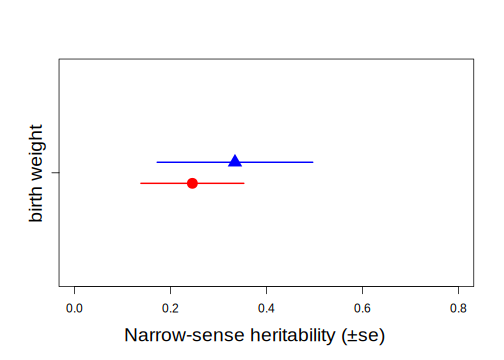
\includegraphics{wam_tuto_files/figure-latex/unnamed-chunk-27-1.pdf}
\caption{\label{fig:unnamed-chunk-27}Female and male heritability of birth weight}
\end{figure}

\hypertarget{modification-of-the-varaince-matrix-parameters}{%
\subsection{Modification of the varaince matrix parameters}\label{modification-of-the-varaince-matrix-parameters}}

Variance represents the deviation of the distribution and it expected to be a positive values.
Due to a lack of power, a structural problem in the dataset or a very low variance, Asreml-r often fixes the variance to a boundary \texttt{B} instead of a positive value \texttt{P}. When it is happen, it is generally a good idea to examine it.

To examine the boundary effect, we can explore an alternative model where the model allowed a unstructured parameter for the variance of interest or the entire variance matrix. For this example: we allowed the model to estimate any values (so allowing possible negative values of estimates) for the random and residual matrix.

First, we create a temporary model \texttt{model.temp} with the exact structure to modify.

\begin{Shaded}
\begin{Highlighting}[]
\NormalTok{model.temp \textless{}{-}}\StringTok{ }\KeywordTok{asreml}\NormalTok{(}
  \DataTypeTok{fixed =}\NormalTok{ bwt }\OperatorTok{\textasciitilde{}}\StringTok{ }\DecValTok{1}\NormalTok{,}
  \DataTypeTok{random =} \OperatorTok{\textasciitilde{}}\StringTok{ }\KeywordTok{vm}\NormalTok{(animal, ainv) }\OperatorTok{+}\StringTok{ }\NormalTok{byear }\OperatorTok{+}\StringTok{ }\NormalTok{mother,}
  \DataTypeTok{residual =} \OperatorTok{\textasciitilde{}}\StringTok{ }\KeywordTok{idv}\NormalTok{(units),}
  \DataTypeTok{data =}\NormalTok{ gryphon,}
  \DataTypeTok{na.action =} \KeywordTok{na.method}\NormalTok{(}\DataTypeTok{x =} \StringTok{"omit"}\NormalTok{, }\DataTypeTok{y =} \StringTok{"omit"}\NormalTok{),}
  \DataTypeTok{start.values =}\NormalTok{ T}
\NormalTok{)}
\NormalTok{G.temp \textless{}{-}}\StringTok{ }\NormalTok{model.temp}\OperatorTok{$}\NormalTok{vparameters[(}\DecValTok{1}\OperatorTok{:}\DecValTok{3}\NormalTok{), ]}
\NormalTok{G.temp}\OperatorTok{$}\NormalTok{Constraint \textless{}{-}}\StringTok{ "U"}
\NormalTok{R.temp \textless{}{-}}\StringTok{ }\NormalTok{model.temp}\OperatorTok{$}\NormalTok{vparameters[}\OperatorTok{{-}}\NormalTok{(}\DecValTok{1}\OperatorTok{:}\DecValTok{3}\NormalTok{), ]}
\NormalTok{R.temp}\OperatorTok{$}\NormalTok{Constraint[}\DecValTok{2}\NormalTok{] \textless{}{-}}\StringTok{ "U"}
\end{Highlighting}
\end{Shaded}

The argument \texttt{start.values=T} allowed the \texttt{model.temp} to change its random parameters. We can create the two different matrices and specify which parameters will be modified. For this example we modified the G and the R matrix to fit all variance to be \texttt{U} unstructured. it is important to note for the R matrix the line \texttt{units!R} has to be fix to 1, so it will never change.

The object G.temp and R.temp can be implemented in the following model as new parameters using the argument \texttt{R.param} and \texttt{G.param}.

\begin{Shaded}
\begin{Highlighting}[]
\NormalTok{model5 \textless{}{-}}\StringTok{ }\KeywordTok{asreml}\NormalTok{(}
  \DataTypeTok{fixed =}\NormalTok{ bwt }\OperatorTok{\textasciitilde{}}\StringTok{ }\DecValTok{1} \OperatorTok{+}\StringTok{ }\NormalTok{sex,}
  \DataTypeTok{random =} \OperatorTok{\textasciitilde{}}\StringTok{ }\KeywordTok{vm}\NormalTok{(animal, ainv) }\OperatorTok{+}\StringTok{ }\NormalTok{byear }\OperatorTok{+}\StringTok{ }\NormalTok{mother,}
  \DataTypeTok{residual =} \OperatorTok{\textasciitilde{}}\StringTok{ }\KeywordTok{idv}\NormalTok{(units),}
  \DataTypeTok{data =}\NormalTok{ gryphon,}
  \DataTypeTok{na.action =} \KeywordTok{na.method}\NormalTok{(}\DataTypeTok{x =} \StringTok{"omit"}\NormalTok{, }\DataTypeTok{y =} \StringTok{"omit"}\NormalTok{),}
  \DataTypeTok{R.param =}\NormalTok{ R.temp, }\DataTypeTok{G.param =}\NormalTok{ G.temp}
\NormalTok{)}
\end{Highlighting}
\end{Shaded}

\begin{verbatim}
## Model fitted using the sigma parameterization.
## ASReml 4.1.0 Sat Apr 30 11:04:17 2022
##           LogLik        Sigma2     DF     wall    cpu
##  1     -2033.178           1.0    852 11:04:17    0.0
##  2     -1723.734           1.0    852 11:04:17    0.0
##  3     -1396.354           1.0    852 11:04:17    0.0
##  4     -1193.012           1.0    852 11:04:17    0.0
##  5     -1107.946           1.0    852 11:04:17    0.0
##  6     -1095.327           1.0    852 11:04:17    0.0
##  7     -1094.816           1.0    852 11:04:17    0.0
##  8     -1094.815           1.0    852 11:04:17    0.0
\end{verbatim}

\begin{Shaded}
\begin{Highlighting}[]
\KeywordTok{summary}\NormalTok{(model5)}\OperatorTok{$}\NormalTok{varcomp}
\end{Highlighting}
\end{Shaded}

\begin{verbatim}
##                  component std.error  z.ratio bound %ch
## byear            0.8820313 0.2632455 3.350604     U   0
## mother           1.1184698 0.2386239 4.687167     U   0
## vm(animal, ainv) 2.2985320 0.4962496 4.631806     U   0
## units!units      1.6290034 0.3714154 4.385934     U   0
## units!R          1.0000000        NA       NA     F   0
\end{verbatim}

Since \texttt{model4} did not showed boundary, \texttt{the\ model5} is very similar.

\hypertarget{covariance-between-two-random-effects}{%
\subsection{Covariance between two random effects}\label{covariance-between-two-random-effects}}

Some research questions require to estimate the covariance between two random effects within a univariate model.To do so, we can use the argument \texttt{str}.
As an example, we fit a model which estimate the covariance between the additive genetic variance and the mother variance. Both variances require to operate on the same level, thus \texttt{animal} and \texttt{mother} require to be associated to the pedigree information.

The argument \texttt{str}has two components: first the equation term with the two random effects \texttt{\textasciitilde{}vm(animal,Ainv)+vm(mother,\ ainv)} and second the structural term \texttt{\textasciitilde{}us(2):id(number)}. Here within the structural term, we fit a 2x2 unstructured matrix \texttt{us(2)} which estimated the variance and the covariance between the random effects in the equation term.
To successfully work, the structural term also requires the number of level identified within \texttt{id()}. Here a small tip, if you don't know the number of level identified within id(), run the model with a random number. The model will not converge and a error message will appear like this one: \texttt{Size\ of\ direct\ product\ (4)\ does\ not\ conform\ with\ total\ size\ of\ included\ terms\ (2618)}. The error message can help you determine the required level within the \texttt{str} function, as here 2618 divide by 2.
In addition, it is necessary the random effects

\begin{Shaded}
\begin{Highlighting}[]
\NormalTok{model.temp2 \textless{}{-}}\StringTok{ }\KeywordTok{asreml}\NormalTok{(}
  \DataTypeTok{fixed =}\NormalTok{ bwt }\OperatorTok{\textasciitilde{}}\StringTok{ }\DecValTok{1}\NormalTok{,}
  \DataTypeTok{random =} \OperatorTok{\textasciitilde{}}\StringTok{ }\KeywordTok{str}\NormalTok{(}\OperatorTok{\textasciitilde{}}\StringTok{ }\KeywordTok{vm}\NormalTok{(animal, ainv) }\OperatorTok{+}\StringTok{ }\KeywordTok{vm}\NormalTok{(mother, ainv), }\OperatorTok{\textasciitilde{}}\StringTok{ }\KeywordTok{us}\NormalTok{(}\DecValTok{2}\NormalTok{)}\OperatorTok{:}\KeywordTok{id}\NormalTok{(}\DecValTok{1309}\NormalTok{)) }\OperatorTok{+}\StringTok{ }\NormalTok{byear,}
  \DataTypeTok{residual =} \OperatorTok{\textasciitilde{}}\StringTok{ }\KeywordTok{idv}\NormalTok{(units),}
  \DataTypeTok{data =}\NormalTok{ gryphon,}
  \DataTypeTok{na.action =} \KeywordTok{na.method}\NormalTok{(}\DataTypeTok{x =} \StringTok{"omit"}\NormalTok{, }\DataTypeTok{y =} \StringTok{"omit"}\NormalTok{),}
  \DataTypeTok{start.values =}\NormalTok{ T}
\NormalTok{)}

\NormalTok{G.temp2 \textless{}{-}}\StringTok{ }\NormalTok{model.temp2}\OperatorTok{$}\NormalTok{vparameters[(}\DecValTok{1}\OperatorTok{:}\DecValTok{4}\NormalTok{), ]}
\NormalTok{G.temp2}\OperatorTok{$}\NormalTok{Constraint \textless{}{-}}\StringTok{ "U"}
\NormalTok{model6 \textless{}{-}}\StringTok{ }\KeywordTok{asreml}\NormalTok{(}
  \DataTypeTok{fixed =}\NormalTok{ bwt }\OperatorTok{\textasciitilde{}}\StringTok{ }\DecValTok{1} \OperatorTok{+}\StringTok{ }\NormalTok{sex,}
  \DataTypeTok{random =} \OperatorTok{\textasciitilde{}}\StringTok{ }\KeywordTok{str}\NormalTok{(}\OperatorTok{\textasciitilde{}}\StringTok{ }\KeywordTok{vm}\NormalTok{(animal, ainv) }\OperatorTok{+}\StringTok{ }\KeywordTok{vm}\NormalTok{(mother, ainv), }\OperatorTok{\textasciitilde{}}\StringTok{ }\KeywordTok{us}\NormalTok{(}\DecValTok{2}\NormalTok{)}\OperatorTok{:}\KeywordTok{id}\NormalTok{(}\DecValTok{1309}\NormalTok{)) }\OperatorTok{+}\StringTok{ }\NormalTok{byear,}
  \DataTypeTok{residual =} \OperatorTok{\textasciitilde{}}\StringTok{ }\KeywordTok{idv}\NormalTok{(units),}
  \DataTypeTok{data =}\NormalTok{ gryphon,}
  \DataTypeTok{na.action =} \KeywordTok{na.method}\NormalTok{(}\DataTypeTok{x =} \StringTok{"omit"}\NormalTok{, }\DataTypeTok{y =} \StringTok{"omit"}\NormalTok{),}
  \CommentTok{\# equate.levels = c("animal", "mother"),}
\NormalTok{  , }\DataTypeTok{G.param =}\NormalTok{ G.temp2}
\NormalTok{)}
\KeywordTok{summary}\NormalTok{(model6)}\OperatorTok{$}\NormalTok{varcomp}
\end{Highlighting}
\end{Shaded}

We have successfully produced a code to estimate the covariance between two random effects. However for this example, the dataset is not sufficient to properly estimate it and the model did not converge but you have the idea of how to use the function \texttt{str}.

Additional and final tip: It is happen that Asreml will estimate negative variance if you allow the variance matrix to be unstructured. A negative variance is counter-intuitive meaning statistically the mean within the random effect is less similar than expected by chance.
However a possible biological reason can be hypothesized such as a sibling competition within the nest creating a negative among-individual covariance within the nest.Thus to test this hypotheses,it is required to estimate the covariance between two random effects.

\hypertarget{gremlin-1}{%
\section{gremlin}\label{gremlin-1}}

TODO (maybe just bother Matthew to do it)

Meanwhile

\begin{figure}

\includegraphics[width=1\linewidth]{images/Gizmo} \caption{Keep it dry and do no feed after midnight.}\label{fig:unnamed-chunk-31}
\end{figure}

\hypertarget{mcmcglmm-1}{%
\section{MCMCglmm}\label{mcmcglmm-1}}

\hypertarget{running-the-model-1}{%
\subsection{Running the model}\label{running-the-model-1}}

First load MCMCglmm:

\begin{Shaded}
\begin{Highlighting}[]
\KeywordTok{library}\NormalTok{(MCMCglmm)}
\end{Highlighting}
\end{Shaded}

The first model we will fit is a simple animal model with no fixed effects, and only an `animal' random effect relating individuals to their additive genetic values through the pedigree.

First we are going to define the priors. In a way we might want to avoid using priors, because we would like all of the information in our analysis to come from our data.
By default MCMCglmm uses improper priors, but this can cause inferential and numerical problems. We will specify priors for the animal effect and the residual variance using the following code:

\begin{Shaded}
\begin{Highlighting}[]
\NormalTok{prior1}\FloatTok{.1}\NormalTok{ \textless{}{-}}\StringTok{ }\KeywordTok{list}\NormalTok{(}
  \DataTypeTok{G =} \KeywordTok{list}\NormalTok{(}\DataTypeTok{G1 =} \KeywordTok{list}\NormalTok{(}\DataTypeTok{V =} \DecValTok{1}\NormalTok{, }\DataTypeTok{nu =} \FloatTok{0.002}\NormalTok{)),}
  \DataTypeTok{R =} \KeywordTok{list}\NormalTok{(}\DataTypeTok{V =} \DecValTok{1}\NormalTok{, }\DataTypeTok{nu =} \FloatTok{0.002}\NormalTok{)}
\NormalTok{)}
\end{Highlighting}
\end{Shaded}

A prior allowed the model to fit different variance structures. With the unique random effect ``animal'', we partitioned the phenotypic variance into two distinct variances matrices \texttt{G} (additive genetic) and \texttt{R} (residual).
This prior specification is the simplistic one and often used because it was believed to be relatively uninformative, and is equivalent to an inverse-gamma prior with shape and scale equal to 0.001. In many cases it is relatively uninformative but when the posterior distribution for the variances has support close to zero it can behave poorly. Parameter expanded priors (See Chapter 8 of the MCMCglmm CourseNotes, available from CRAN) are gaining in popularity due to their better behaviour but for the purposes of this tutorial we will stick with the inverse-gamma prior.

We have told MCMCglmm to pay little heed to our prior expectation (V) by specifying a small degree of belief parameter (nu) of 0.002. Since this is a univariate analysis, the priors are matrix of order 1 and thus nu\textgreater0 is the smallest degree of belief that provides what is known as a `proper' prior, avoiding numerical problems. In fact, there is a lot of information in the data regarding the marginal distributions of the parameters, and MCMCglmm will run most of the models that we suggest in these tutorials without priors. However, this is poor practice, but we will therefore use this simple priors throughout these tutorials. We can now fit an animal model. The model to decompose variation in birth weight into genetic and residual effects is as follows:

The lower case ``animal'' is a can be a \textbf{special} word for MCMCglmm. If a \texttt{pedigree} argument is provided then \texttt{MCMCglmm} will recognize the term \texttt{animal} as the term to use to estimate additive genetic variance. When the argument \texttt{pedigree} is not provided then the word \texttt{animal} is not different than any other variable. However, instead of providing a pedigree argument to the call to MCMCglmm function, it is much more flexible to use the \texttt{ginv} argument to specify the random effect that must be linked to the pedigree (with the inverse relatedness matrix). We thus first estimate the inverse relatedness matrix using \texttt{inverseA()} then fit the animal model.

\begin{Shaded}
\begin{Highlighting}[]
\NormalTok{Ainv \textless{}{-}}\StringTok{ }\KeywordTok{inverseA}\NormalTok{(gryphonped)}\OperatorTok{$}\NormalTok{Ainv}
\NormalTok{model1}\FloatTok{.1}\NormalTok{ \textless{}{-}}\StringTok{ }\KeywordTok{MCMCglmm}\NormalTok{(bwt }\OperatorTok{\textasciitilde{}}\StringTok{ }\DecValTok{1}\NormalTok{,}
  \DataTypeTok{random =} \OperatorTok{\textasciitilde{}}\NormalTok{animal, }\DataTypeTok{ginv =} \KeywordTok{list}\NormalTok{(}\DataTypeTok{animal =}\NormalTok{ Ainv),}
  \DataTypeTok{data =}\NormalTok{ gryphon, }\DataTypeTok{prior =}\NormalTok{ prior1}\FloatTok{.1}
\NormalTok{)}
\end{Highlighting}
\end{Shaded}

\begin{verbatim}
## 
##                        MCMC iteration = 0
## 
##                        MCMC iteration = 1000
## 
##                        MCMC iteration = 2000
## 
##                        MCMC iteration = 3000
## 
##                        MCMC iteration = 4000
## 
##                        MCMC iteration = 5000
## 
##                        MCMC iteration = 6000
## 
##                        MCMC iteration = 7000
## 
##                        MCMC iteration = 8000
## 
##                        MCMC iteration = 9000
## 
##                        MCMC iteration = 10000
## 
##                        MCMC iteration = 11000
## 
##                        MCMC iteration = 12000
## 
##                        MCMC iteration = 13000
\end{verbatim}

After typing this code, MCMCglmm will run, taking about 20 seconds on a modern desktop computer. The progress of the run will be printed to the screen. Also, note the warning message will be printed at the end of the run. This is natural too. In order for the MCMC algorithm to work, MCMCglmm must keep track of effects associated with unmeasured individuals appearing in the pedigree. This will not affect the answers, but when many unmeasured individuals exist, it can hinder the ability of the algorithm to explore the parameter space (more on this, and a solution, later). Lets have a look at the MCMCglmm outputs. First we will evaluate how confident we can be that MCMCglmm found good answers. By entering

\begin{Shaded}
\begin{Highlighting}[]
\KeywordTok{plot}\NormalTok{(model1}\FloatTok{.1}\OperatorTok{$}\NormalTok{Sol)}
\end{Highlighting}
\end{Shaded}

\begin{figure}
\centering
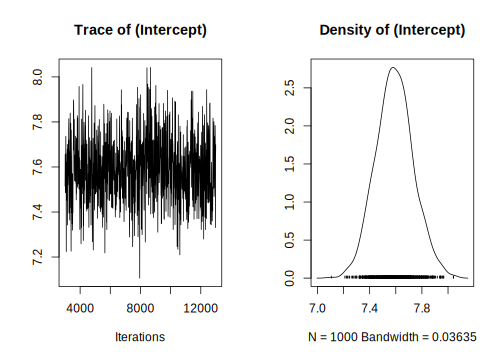
\includegraphics{wam_tuto_files/figure-latex/unnamed-chunk-35-1.pdf}
\caption{\label{fig:unnamed-chunk-35}The posterior distribution of the fixed effect (the intercept, or mean) in model 1.1}
\end{figure}

in the console, we get Figure 2.2. The plot on the left shows a time series of the values of 1000 samples of the posterior distribution of the the model intercept (mean birth weight). The plot on the right shows the same data as a distribution. Complicated statistical methods for estimating population means are of course of little interest; rather, we are examining these outputs to check that MCMCglmm's algorithms worked well for our data and for this model. The important point here is that a consistent amount of variation around a largely unchanging mean value of the intercept was obtained (which give this fluctuating trace concentrated around the mean), and the posterior distribution of the intercept appears to be valid. More rigorous means of evaluation the independence of the samples in the posterior distribution (evaluating autocorrelation) are discussed in the MCMCglmm CourseNotes, available from CRAN. Note that your output for \texttt{model\ 1.1} may not be identical to this due to Monte Carlo (random number) error. So every times, you run the model, you will get similar but slightly different results.

The posterior distributions of the the variance components are generally of more interest to animal model users. We can view plots of the posterior distribution for the variance components for model 1.1 by

\begin{Shaded}
\begin{Highlighting}[]
\KeywordTok{plot}\NormalTok{(model1}\FloatTok{.1}\OperatorTok{$}\NormalTok{VCV)}
\end{Highlighting}
\end{Shaded}

\begin{figure}
\centering
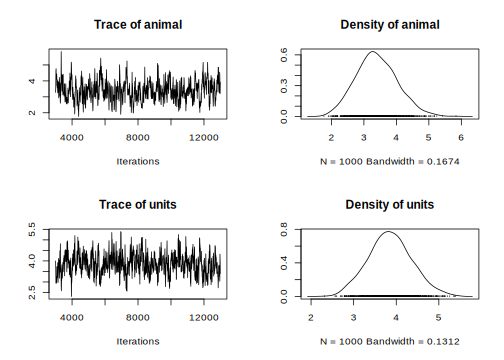
\includegraphics{wam_tuto_files/figure-latex/unnamed-chunk-36-1.pdf}
\caption{\label{fig:unnamed-chunk-36}The posterior distributions of the variance components of model 1.1, based on an analysis with the default values for nitt, burnin, and thin in MCMCglmm}
\end{figure}

which generates Figure 2.3. Here we see distributions of the estimates of the additive genetic (animal) and residual (units) effects. These samples contain some autocorrelation, i.e., trends are apparent in the left-hand plot. We can deal with this easily.

\hypertarget{change-in-iteration-and-sampling}{%
\subsection{Change in iteration and sampling}\label{change-in-iteration-and-sampling}}

We will simply re-run the model for a longer number of iterations, and sample the chain less frequently. So far we have been running MCMCglmm with its default values. These defaults are a total run length of 13000 iterations, the first 3000 of which are discarded as a `burn-in' period to make sure that the converges to the part of the parameter space where the maximum likelihood exists. The remaining 10000 iterations are sampled (estimates retained) every 10 iterations (the thinning interval). Because the values in the left-hand plots in figure 2.2 to appear to have different values at the beginning of the run, we might suspect that a longer burn-in period might be required. We can reduce the autocorrelation by lengthening the rest of the run and sampling the chain less frequently. The following code runs the same model 1.1, but is likely to produce better samples of the posterior distributions. This model should take about two minutes to analyze.

\begin{Shaded}
\begin{Highlighting}[]
\NormalTok{model1}\FloatTok{.1}\NormalTok{ \textless{}{-}}\StringTok{ }\KeywordTok{MCMCglmm}\NormalTok{(bwt }\OperatorTok{\textasciitilde{}}\StringTok{ }\DecValTok{1}\NormalTok{,}
  \DataTypeTok{random =} \OperatorTok{\textasciitilde{}}\NormalTok{animal, }\DataTypeTok{ginv =} \KeywordTok{list}\NormalTok{(}\DataTypeTok{animal =}\NormalTok{ Ainv),}
  \DataTypeTok{data =}\NormalTok{ gryphon, }\DataTypeTok{nitt =} \DecValTok{65000}\NormalTok{, }\DataTypeTok{thin =} \DecValTok{50}\NormalTok{, }\DataTypeTok{burnin =} \DecValTok{15000}\NormalTok{,}
  \DataTypeTok{prior =}\NormalTok{ prior1}\FloatTok{.1}\NormalTok{, }\DataTypeTok{verbose =} \OtherTok{FALSE}
\NormalTok{)}
\end{Highlighting}
\end{Shaded}

Notes that we have now included the argument verbose=FALSE in the MCMCglmm call. We will continue this throughout the tutorial so that more complete screen outputs can be included in this document without using too much space.Note that the autocorrelation is much reduced. A more compact way to evaluate the validity of the posterior distributions is to calculate autocorrelation among samples, as follows:

\begin{Shaded}
\begin{Highlighting}[]
\KeywordTok{autocorr.diag}\NormalTok{(model1}\FloatTok{.1}\OperatorTok{$}\NormalTok{VCV)}
\end{Highlighting}
\end{Shaded}

\begin{verbatim}
##                animal        units
## Lag 0     1.000000000  1.000000000
## Lag 50    0.209039004  0.173955831
## Lag 250  -0.017811690 -0.028870690
## Lag 500  -0.007328492  0.008719608
## Lag 2500  0.050325531  0.056367451
\end{verbatim}

We will consider these levels of autocorrelation acceptable, at least for the purposes of this tutorial. Ideally, all samples of the posterior distribution should be independent, and the autocorrelation for all lag values greater than zero should be near zero. However, in practice this will not strictly be achievable for all analytic scenarios. Certainly the levels of autocorrelation observed here should not be tolerated in any formal analysis.
Note that the validity of posterior distributions of any analysis should always be checked; however, for brevity we will not continue to be so consistently diligent throughout the rest of these tutorials. We can now proceed with confidence to recover some more information from these samples. We can obtain estimates of the additive genetic and residual variance by calculating the modes of the posterior distributions:

\begin{Shaded}
\begin{Highlighting}[]
\KeywordTok{posterior.mode}\NormalTok{(model1}\FloatTok{.1}\OperatorTok{$}\NormalTok{VCV)}
\end{Highlighting}
\end{Shaded}

\begin{verbatim}
##   animal    units 
## 3.310074 3.728226
\end{verbatim}

We can obtain the Bayesian equivalent of confidence intervals by calculating the the values of the estimates that bound 95\% (or any other proportion) of the posterior distributions:

\begin{Shaded}
\begin{Highlighting}[]
\KeywordTok{HPDinterval}\NormalTok{(model1}\FloatTok{.1}\OperatorTok{$}\NormalTok{VCV)}
\end{Highlighting}
\end{Shaded}

\begin{verbatim}
##           lower    upper
## animal 2.185154 4.567025
## units  2.899000 4.922814
## attr(,"Probability")
## [1] 0.95
\end{verbatim}

\hypertarget{change-priors-parameters}{%
\subsection{Change priors parameters}\label{change-priors-parameters}}

We specified weak priors in this analyses. Now we will check whether or not proper priors would have influenced the results that we obtained. The simplest way to do this is to re-run the model with different priors.
In the previous model we specified a prior where the size of genetic and residual variance were similar. Here we construct priors with a larger degree of belief parameter (\texttt{nu}), and we will specify that a large proportion (95\%) of the variation is under genetic control (\texttt{V}).Thus, the residual variance contains 05\% of the phenotypic variance.

\begin{Shaded}
\begin{Highlighting}[]
\NormalTok{p.var \textless{}{-}}\StringTok{ }\KeywordTok{var}\NormalTok{(gryphon}\OperatorTok{$}\NormalTok{bwt, }\DataTypeTok{na.rm =} \OtherTok{TRUE}\NormalTok{)}
\NormalTok{prior1.}\FloatTok{1.2}\NormalTok{ \textless{}{-}}\StringTok{ }\KeywordTok{list}\NormalTok{(}
  \DataTypeTok{G =} \KeywordTok{list}\NormalTok{(}\DataTypeTok{G1 =} \KeywordTok{list}\NormalTok{(}\DataTypeTok{V =} \KeywordTok{matrix}\NormalTok{(p.var }\OperatorTok{*}\StringTok{ }\FloatTok{0.95}\NormalTok{), }\DataTypeTok{nu =} \DecValTok{1}\NormalTok{)),}
  \DataTypeTok{R =} \KeywordTok{list}\NormalTok{(}\DataTypeTok{V =} \KeywordTok{matrix}\NormalTok{(p.var }\OperatorTok{*}\StringTok{ }\FloatTok{0.05}\NormalTok{), }\DataTypeTok{nu =} \DecValTok{1}\NormalTok{)}
\NormalTok{)}

\NormalTok{model1.}\FloatTok{1.2}\NormalTok{ \textless{}{-}}\StringTok{ }\KeywordTok{MCMCglmm}\NormalTok{(bwt }\OperatorTok{\textasciitilde{}}\StringTok{ }\DecValTok{1}\NormalTok{,}
  \DataTypeTok{random =} \OperatorTok{\textasciitilde{}}\NormalTok{animal, }\DataTypeTok{ginv =} \KeywordTok{list}\NormalTok{(}\DataTypeTok{animal =}\NormalTok{ Ainv),}
  \DataTypeTok{data =}\NormalTok{ gryphon, }\DataTypeTok{prior =}\NormalTok{ prior1.}\FloatTok{1.2}\NormalTok{, }\DataTypeTok{nitt =} \DecValTok{65000}\NormalTok{, }\DataTypeTok{thin =} \DecValTok{50}\NormalTok{,}
  \DataTypeTok{burnin =} \DecValTok{15000}\NormalTok{, }\DataTypeTok{verbose =} \OtherTok{FALSE}
\NormalTok{)}
\KeywordTok{posterior.mode}\NormalTok{(model1}\FloatTok{.1}\OperatorTok{$}\NormalTok{VCV)}
\end{Highlighting}
\end{Shaded}

\begin{verbatim}
##   animal    units 
## 3.310074 3.728226
\end{verbatim}

\begin{Shaded}
\begin{Highlighting}[]
\KeywordTok{posterior.mode}\NormalTok{(model1.}\FloatTok{1.2}\OperatorTok{$}\NormalTok{VCV)}
\end{Highlighting}
\end{Shaded}

\begin{verbatim}
##   animal    units 
## 3.299524 4.026746
\end{verbatim}

and we can therefore conclude that the difference in the priors has little effect on the outcome of the analysis. This is typical for an analysis where lots of data are available relative to the complexity of the model, but is often not the case. In all cases, it is important to check the effect of priors on conclusions drawn from a model. In addition, you can also specify the prior with previous knowledge or expectation for the variance.

\hypertarget{estimating-heritability-1}{%
\subsection{Estimating heritability}\label{estimating-heritability-1}}

A useful property of Bayesian posterior distributions is that we can apply almost any transformation to these distributions and they will remain valid. This applies to the calculation of heritability. We can obtain an estimate of the heritability by applying the basic formula \(h^2\) =\(V_A /V_P\) to each sample of the posterior distribution:

\begin{Shaded}
\begin{Highlighting}[]
\NormalTok{posterior.heritability1}\FloatTok{.1}\NormalTok{ \textless{}{-}}\StringTok{ }\NormalTok{model1}\FloatTok{.1}\OperatorTok{$}\NormalTok{VCV[, }\StringTok{"animal"}\NormalTok{] }\OperatorTok{/}
\StringTok{  }\NormalTok{(model1}\FloatTok{.1}\OperatorTok{$}\NormalTok{VCV[, }\StringTok{"animal"}\NormalTok{] }\OperatorTok{+}\StringTok{ }\NormalTok{model1}\FloatTok{.1}\OperatorTok{$}\NormalTok{VCV[, }\StringTok{"units"}\NormalTok{])}

\KeywordTok{posterior.mode}\NormalTok{(posterior.heritability1}\FloatTok{.1}\NormalTok{)}
\end{Highlighting}
\end{Shaded}

\begin{verbatim}
##      var1 
## 0.4603614
\end{verbatim}

\begin{Shaded}
\begin{Highlighting}[]
\KeywordTok{HPDinterval}\NormalTok{(posterior.heritability1}\FloatTok{.1}\NormalTok{, }\FloatTok{0.95}\NormalTok{)}
\end{Highlighting}
\end{Shaded}

\begin{verbatim}
##          lower     upper
## var1 0.3236453 0.6079976
## attr(,"Probability")
## [1] 0.95
\end{verbatim}

Generate a plot of the posterior distribution of this heritability estimate:

\begin{Shaded}
\begin{Highlighting}[]
\KeywordTok{plot}\NormalTok{(posterior.heritability1}\FloatTok{.1}\NormalTok{)}
\end{Highlighting}
\end{Shaded}

\begin{figure}
\centering
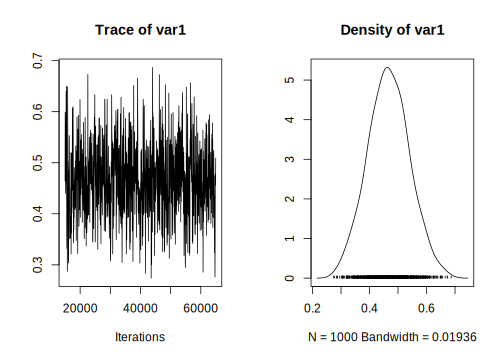
\includegraphics{wam_tuto_files/figure-latex/unnamed-chunk-43-1.pdf}
\caption{\label{fig:unnamed-chunk-43}The posterior distributions the heritability from model 1.1}
\end{figure}

\hypertarget{adding-fixed-effects-1}{%
\subsection{Adding fixed effects}\label{adding-fixed-effects-1}}

To add effects to a univariate model, we simply modify the fixed effect part of the model specification:

\begin{Shaded}
\begin{Highlighting}[]
\NormalTok{model1}\FloatTok{.2}\NormalTok{ \textless{}{-}}\StringTok{ }\KeywordTok{MCMCglmm}\NormalTok{(bwt }\OperatorTok{\textasciitilde{}}\StringTok{ }\NormalTok{sex,}
  \DataTypeTok{random =} \OperatorTok{\textasciitilde{}}\NormalTok{animal, }\DataTypeTok{ginv =} \KeywordTok{list}\NormalTok{(}\DataTypeTok{animal =}\NormalTok{ Ainv),}
  \DataTypeTok{data =}\NormalTok{ gryphon, }\DataTypeTok{prior =}\NormalTok{ prior1}\FloatTok{.1}\NormalTok{,}
  \DataTypeTok{nitt =} \DecValTok{65000}\NormalTok{, }\DataTypeTok{thin =} \DecValTok{50}\NormalTok{, }\DataTypeTok{burnin =} \DecValTok{15000}\NormalTok{, }\DataTypeTok{verbose =} \OtherTok{FALSE}
\NormalTok{)}
\KeywordTok{summary}\NormalTok{(model1}\FloatTok{.2}\NormalTok{)}
\end{Highlighting}
\end{Shaded}

\begin{verbatim}
## 
##  Iterations = 15001:64951
##  Thinning interval  = 50
##  Sample size  = 1000 
## 
##  DIC: 3719.3 
## 
##  G-structure:  ~animal
## 
##        post.mean l-95% CI u-95% CI eff.samp
## animal     3.049    2.093    4.092    716.9
## 
##  R-structure:  ~units
## 
##       post.mean l-95% CI u-95% CI eff.samp
## units     2.974    2.168     3.74    775.5
## 
##  Location effects: bwt ~ sex 
## 
##             post.mean l-95% CI u-95% CI eff.samp  pMCMC    
## (Intercept)     6.053    5.726    6.359     1201 <0.001 ***
## sex2            2.214    1.895    2.536     1000 <0.001 ***
## ---
## Signif. codes:  0 '***' 0.001 '**' 0.01 '*' 0.05 '.' 0.1 ' ' 1
\end{verbatim}

We can assess the significance of \texttt{sex} as a fixed effect by examining its posterior distribution. Important notes here, it is important to know how the model names their fixed effect level to call them properly.

\begin{Shaded}
\begin{Highlighting}[]
\KeywordTok{posterior.mode}\NormalTok{(model1}\FloatTok{.2}\OperatorTok{$}\NormalTok{Sol[, }\StringTok{"sex2"}\NormalTok{])}
\end{Highlighting}
\end{Shaded}

\begin{verbatim}
##    var1 
## 2.16871
\end{verbatim}

\begin{Shaded}
\begin{Highlighting}[]
\KeywordTok{HPDinterval}\NormalTok{(model1}\FloatTok{.2}\OperatorTok{$}\NormalTok{Sol[, }\StringTok{"sex2"}\NormalTok{], }\FloatTok{0.95}\NormalTok{)}
\end{Highlighting}
\end{Shaded}

\begin{verbatim}
##        lower    upper
## var1 1.89504 2.536397
## attr(,"Probability")
## [1] 0.95
\end{verbatim}

The posterior distribution of the \texttt{sex2} term does not overlap zero. Thus, we can infer that sex has an effect on birth weight (presence of a sexual dimorphism) in this model and is a useful addition to the model, for most purposes. It is also worth noting that the variance components have changed slightly:

\begin{Shaded}
\begin{Highlighting}[]
\KeywordTok{posterior.mode}\NormalTok{(model1}\FloatTok{.2}\OperatorTok{$}\NormalTok{VCV)}
\end{Highlighting}
\end{Shaded}

\begin{verbatim}
##   animal    units 
## 2.960190 3.117091
\end{verbatim}

In fact since sex effects were previously contributing to the residual variance of the model our estimate of \(V_R\) (denoted 'units' in the output) is now slightly lower than before. This has an important consequence for estimating heritability since if we calculate \(V_P\) as \(V_A +V_R\) then as we include fixed effects we will soak up more residual variance driving \(V_P\) . Assuming that \(V_A\) is more or less unaffected by the fixed effects fitted then as \(V_P\) goes down we expect our estimate of \(h^2\) will go up.

\begin{Shaded}
\begin{Highlighting}[]
\NormalTok{posterior.heritability1}\FloatTok{.2}\NormalTok{ \textless{}{-}}\StringTok{ }\NormalTok{model1}\FloatTok{.2}\OperatorTok{$}\NormalTok{VCV[, }\StringTok{"animal"}\NormalTok{] }\OperatorTok{/}
\StringTok{  }\NormalTok{(model1}\FloatTok{.2}\OperatorTok{$}\NormalTok{VCV[, }\StringTok{"animal"}\NormalTok{] }\OperatorTok{+}\StringTok{ }\NormalTok{model1}\FloatTok{.2}\OperatorTok{$}\NormalTok{VCV[, }\StringTok{"units"}\NormalTok{])}
\KeywordTok{posterior.mode}\NormalTok{(posterior.heritability1}\FloatTok{.2}\NormalTok{)}
\end{Highlighting}
\end{Shaded}

\begin{verbatim}
##      var1 
## 0.4915129
\end{verbatim}

\begin{Shaded}
\begin{Highlighting}[]
\KeywordTok{HPDinterval}\NormalTok{(posterior.heritability1}\FloatTok{.2}\NormalTok{, }\FloatTok{0.95}\NormalTok{)}
\end{Highlighting}
\end{Shaded}

\begin{verbatim}
##         lower     upper
## var1 0.364643 0.6437182
## attr(,"Probability")
## [1] 0.95
\end{verbatim}

Here \(h^2\) has increased slightly from 0.4829 to 0.5079 (again, your values may differ slightly due to Monte Carlo error). Which is the better estimate?
It depends on what your question is. The first is an estimate of the proportion of variance in birth weight explained by additive effects, the latter is an estimate of the proportion of variance in birth weight after conditioning on sex that is explained by additive effects.
An important piece of advice, each researcher should be consistent in how they name their estimates and always correctly describe which estimates they are using conditional or not (to avoid any confusion).

\hypertarget{adding-random-effects-1}{%
\subsection{Adding random effects}\label{adding-random-effects-1}}

This is done by simply modifying the model statement in the same way, but requires addition of a prior for the new random effect. For instance, we can fit an effect of birth year:

\begin{Shaded}
\begin{Highlighting}[]
\NormalTok{prior1}\FloatTok{.3}\NormalTok{ \textless{}{-}}\StringTok{ }\KeywordTok{list}\NormalTok{(}
  \DataTypeTok{G =} \KeywordTok{list}\NormalTok{(}\DataTypeTok{G1 =} \KeywordTok{list}\NormalTok{(}\DataTypeTok{V =} \DecValTok{1}\NormalTok{, }\DataTypeTok{nu =} \FloatTok{0.002}\NormalTok{), }\DataTypeTok{G2 =} \KeywordTok{list}\NormalTok{(}\DataTypeTok{V =} \DecValTok{1}\NormalTok{, }\DataTypeTok{nu =} \FloatTok{0.002}\NormalTok{)),}
  \DataTypeTok{R =} \KeywordTok{list}\NormalTok{(}\DataTypeTok{V =} \DecValTok{1}\NormalTok{, }\DataTypeTok{nu =} \FloatTok{0.002}\NormalTok{)}
\NormalTok{)}

\NormalTok{model1}\FloatTok{.3}\NormalTok{ \textless{}{-}}\StringTok{ }\KeywordTok{MCMCglmm}\NormalTok{(bwt }\OperatorTok{\textasciitilde{}}\StringTok{ }\NormalTok{sex,}
  \DataTypeTok{random =} \OperatorTok{\textasciitilde{}}\StringTok{ }\NormalTok{animal }\OperatorTok{+}\StringTok{ }\NormalTok{byear, }\DataTypeTok{ginv =} \KeywordTok{list}\NormalTok{(}\DataTypeTok{animal =}\NormalTok{ Ainv),}
  \DataTypeTok{data =}\NormalTok{ gryphon,}
  \DataTypeTok{nitt =} \DecValTok{65000}\NormalTok{, }\DataTypeTok{thin =} \DecValTok{50}\NormalTok{, }\DataTypeTok{burnin =} \DecValTok{15000}\NormalTok{,}
  \DataTypeTok{prior =}\NormalTok{ prior1}\FloatTok{.3}\NormalTok{, }\DataTypeTok{verbose =} \OtherTok{FALSE}
\NormalTok{)}

\KeywordTok{posterior.mode}\NormalTok{(model1}\FloatTok{.3}\OperatorTok{$}\NormalTok{VCV)}
\end{Highlighting}
\end{Shaded}

\begin{verbatim}
##    animal     byear     units 
## 2.7656801 0.8753865 2.3439002
\end{verbatim}

Here the variance in birth weight explained by birth year is 0.88. Note that although \(V_A\) has changed somewhat, most of what is now partitioned as a \texttt{birth\ year} effect was previously partitioned as \(V_R\) . Thus what we have really done here is to partition environmental effects into those arising from year to year differences versus everything else, and we do not really expect much change in \(h^2\) (since now \(h^2 = V_A /(V_A + V_{BY} + V_R )\)). However, we get a somewhat different result if we also add a random effect of \texttt{mother} to test for maternal effects:

\begin{Shaded}
\begin{Highlighting}[]
\NormalTok{prior1}\FloatTok{.4}\NormalTok{ \textless{}{-}}\StringTok{ }\KeywordTok{list}\NormalTok{(}
  \DataTypeTok{G =} \KeywordTok{list}\NormalTok{(}
    \DataTypeTok{G1 =} \KeywordTok{list}\NormalTok{(}\DataTypeTok{V =} \DecValTok{1}\NormalTok{, }\DataTypeTok{nu =} \FloatTok{0.002}\NormalTok{),}
    \DataTypeTok{G2 =} \KeywordTok{list}\NormalTok{(}\DataTypeTok{V =} \DecValTok{1}\NormalTok{, }\DataTypeTok{nu =} \FloatTok{0.002}\NormalTok{),}
    \DataTypeTok{G3 =} \KeywordTok{list}\NormalTok{(}\DataTypeTok{V =} \DecValTok{1}\NormalTok{, }\DataTypeTok{nu =} \FloatTok{0.002}\NormalTok{)}
\NormalTok{  ),}
  \DataTypeTok{R =} \KeywordTok{list}\NormalTok{(}\DataTypeTok{V =} \DecValTok{1}\NormalTok{, }\DataTypeTok{nu =} \FloatTok{0.002}\NormalTok{)}
\NormalTok{)}

\NormalTok{model1}\FloatTok{.4}\NormalTok{ \textless{}{-}}\StringTok{ }\KeywordTok{MCMCglmm}\NormalTok{(bwt }\OperatorTok{\textasciitilde{}}\StringTok{ }\NormalTok{sex,}
  \DataTypeTok{random =} \OperatorTok{\textasciitilde{}}\StringTok{ }\NormalTok{animal }\OperatorTok{+}\StringTok{ }\NormalTok{byear }\OperatorTok{+}\StringTok{ }\NormalTok{mother,}
  \DataTypeTok{ginv =} \KeywordTok{list}\NormalTok{(}\DataTypeTok{animal =}\NormalTok{ Ainv), }\DataTypeTok{data =}\NormalTok{ gryphon,}
  \DataTypeTok{nitt =} \DecValTok{65000}\NormalTok{, }\DataTypeTok{thin =} \DecValTok{50}\NormalTok{, }\DataTypeTok{burnin =} \DecValTok{15000}\NormalTok{,}
  \DataTypeTok{prior =}\NormalTok{ prior1}\FloatTok{.4}\NormalTok{, }\DataTypeTok{verbose =} \OtherTok{FALSE}
\NormalTok{)}

\KeywordTok{posterior.mode}\NormalTok{(model1}\FloatTok{.4}\OperatorTok{$}\NormalTok{VCV)}
\end{Highlighting}
\end{Shaded}

\begin{verbatim}
##    animal     byear    mother     units 
## 2.5454307 0.7545662 1.0474161 1.8486924
\end{verbatim}

Here partitioning of significant maternal variance has resulted in a further decrease in \(V_R\) but also a decrease in \(V_A\). The latter is because maternal effects of the sort we simulated (fixed differences between mothers) will have the consequence of increasing similarity among maternal siblings. Consequently they can look very much like an additive genetic effects and if present, but unmodelled, represent a type of `common environment effect' that can - and will- cause upward bias in \(V_A\) and so \(h^2\). Let's compare the estimates of heritability from each of models 1.2, 1.3 and 1.4:

\begin{Shaded}
\begin{Highlighting}[]
\NormalTok{posterior.heritability1}\FloatTok{.3}\NormalTok{ \textless{}{-}}\StringTok{ }\NormalTok{model1}\FloatTok{.3}\OperatorTok{$}\NormalTok{VCV[, }\StringTok{"animal"}\NormalTok{] }\OperatorTok{/}
\StringTok{  }\NormalTok{(model1}\FloatTok{.3}\OperatorTok{$}\NormalTok{VCV[, }\StringTok{"animal"}\NormalTok{] }\OperatorTok{+}\StringTok{ }\NormalTok{model1}\FloatTok{.3}\OperatorTok{$}\NormalTok{VCV[, }\StringTok{"byear"}\NormalTok{] }\OperatorTok{+}\StringTok{ }\NormalTok{model1}\FloatTok{.3}\OperatorTok{$}\NormalTok{VCV[, }\StringTok{"units"}\NormalTok{])}
\NormalTok{posterior.heritability1}\FloatTok{.4}\NormalTok{ \textless{}{-}}\StringTok{ }\NormalTok{model1}\FloatTok{.4}\OperatorTok{$}\NormalTok{VCV[, }\StringTok{"animal"}\NormalTok{] }\OperatorTok{/}
\StringTok{  }\NormalTok{(model1}\FloatTok{.4}\OperatorTok{$}\NormalTok{VCV[, }\StringTok{"animal"}\NormalTok{] }\OperatorTok{+}\StringTok{ }\NormalTok{model1}\FloatTok{.4}\OperatorTok{$}\NormalTok{VCV[, }\StringTok{"byear"}\NormalTok{] }\OperatorTok{+}\StringTok{ }\NormalTok{model1}\FloatTok{.4}\OperatorTok{$}\NormalTok{VCV[, }\StringTok{"mother"}\NormalTok{] }\OperatorTok{+}\StringTok{ }\NormalTok{model1}\FloatTok{.4}\OperatorTok{$}\NormalTok{VCV[, }\StringTok{"units"}\NormalTok{])}
\KeywordTok{posterior.mode}\NormalTok{(posterior.heritability1}\FloatTok{.2}\NormalTok{)}
\end{Highlighting}
\end{Shaded}

\begin{verbatim}
##      var1 
## 0.4915129
\end{verbatim}

\begin{Shaded}
\begin{Highlighting}[]
\KeywordTok{posterior.mode}\NormalTok{(posterior.heritability1}\FloatTok{.3}\NormalTok{)}
\end{Highlighting}
\end{Shaded}

\begin{verbatim}
##      var1 
## 0.4536882
\end{verbatim}

\begin{Shaded}
\begin{Highlighting}[]
\KeywordTok{posterior.mode}\NormalTok{(posterior.heritability1}\FloatTok{.4}\NormalTok{)}
\end{Highlighting}
\end{Shaded}

\begin{verbatim}
##      var1 
## 0.3790414
\end{verbatim}

\hypertarget{testing-significance-of-variance-components}{%
\subsection{Testing significance of variance components}\label{testing-significance-of-variance-components}}

While testing the significance of fixed effects by evaluating whether or not their posterior distributions overlap zero was simple and valid, this approach does not work for variance components.
Variance components are bounded to be positive (given a proper prior), and thus even when a random effect is not meaningful, its posterior distribution will never overlap zero. Model comparisons can be performed using the deviance information criterion (\texttt{DIC}), although it should be noted that the properties of DIC are not well understood and that the \texttt{DIC} may be focused at the wrong level for most people's intended level of inference - particularly with non-Gaussian responses. The implementation of \texttt{DIC} in MCMCglmm is further described in the reference manual. \texttt{DIC} values are calculated by MCMCglmm by default. Briefly, \texttt{DIC} like other information criteria balance model fit and model complexity simultaneously, and small values of DIC are preferred. We can compare \texttt{models\ 1.4} and \texttt{1.3}, i.e., models with and without the mother term:

\begin{Shaded}
\begin{Highlighting}[]
\NormalTok{model1}\FloatTok{.3}\OperatorTok{$}\NormalTok{DIC}
\end{Highlighting}
\end{Shaded}

\begin{verbatim}
## [1] 3548.159
\end{verbatim}

\begin{Shaded}
\begin{Highlighting}[]
\NormalTok{model1}\FloatTok{.4}\OperatorTok{$}\NormalTok{DIC}
\end{Highlighting}
\end{Shaded}

\begin{verbatim}
## [1] 3327.724
\end{verbatim}

\texttt{model\ 1.4} has a much lower DIC value. Since the maternal effect term is the only difference between the models, we can consider the inclusion of this term statistically justifiable. We should note however that DIC has a large sampling variance and should probably only be calculated based on much longer MCMC runs.

\hypertarget{further-partitioning-variance}{%
\subsection{Further partitioning variance}\label{further-partitioning-variance}}

A population can be further fragmented into different groups or categories (such as females and males, juveniles and adults or treated and untreated). Some scientific questions require further and deeper analysis of the variance.
To avoid multiple model (one for each group), we can directly partition the variance between groups in a unique model. In addition, by doing so, we can also test if the variance are different between groups.

As example, we can partition the additive genetic variance and residual variance by sex. It is impossible to further partition the other variances but complexity an animal model requires sufficient sample size.

\begin{Shaded}
\begin{Highlighting}[]
\NormalTok{prior1.}\FloatTok{4.}\NormalTok{SEX \textless{}{-}}\StringTok{ }\KeywordTok{list}\NormalTok{(}
  \DataTypeTok{G =} \KeywordTok{list}\NormalTok{(}\DataTypeTok{G1 =} \KeywordTok{list}\NormalTok{(}\DataTypeTok{V =} \KeywordTok{diag}\NormalTok{(}\DecValTok{2}\NormalTok{), }\DataTypeTok{nu =} \FloatTok{1.002}\NormalTok{), }\DataTypeTok{G2 =} \KeywordTok{list}\NormalTok{(}\DataTypeTok{V =} \DecValTok{1}\NormalTok{, }\DataTypeTok{nu =} \FloatTok{0.002}\NormalTok{), }\DataTypeTok{G3 =} \KeywordTok{list}\NormalTok{(}\DataTypeTok{V =} \DecValTok{1}\NormalTok{, }\DataTypeTok{nu =} \FloatTok{0.002}\NormalTok{)),}
  \DataTypeTok{R =} \KeywordTok{list}\NormalTok{(}\DataTypeTok{V =} \KeywordTok{diag}\NormalTok{(}\DecValTok{2}\NormalTok{), }\DataTypeTok{nu =} \FloatTok{1.002}\NormalTok{)}
\NormalTok{)}

\NormalTok{model1.}\FloatTok{4.}\NormalTok{SEX \textless{}{-}}\StringTok{ }\KeywordTok{MCMCglmm}\NormalTok{(bwt }\OperatorTok{\textasciitilde{}}\StringTok{ }\NormalTok{sex,}
  \DataTypeTok{random =} \OperatorTok{\textasciitilde{}}\StringTok{ }\KeywordTok{idh}\NormalTok{(sex)}\OperatorTok{:}\NormalTok{animal }\OperatorTok{+}\StringTok{ }\NormalTok{byear }\OperatorTok{+}\StringTok{ }\NormalTok{mother,}
  \DataTypeTok{rcov =} \OperatorTok{\textasciitilde{}}\StringTok{ }\KeywordTok{idh}\NormalTok{(sex)}\OperatorTok{:}\NormalTok{units,}
  \DataTypeTok{ginv =} \KeywordTok{list}\NormalTok{(}\DataTypeTok{animal =}\NormalTok{ Ainv), }\DataTypeTok{data =}\NormalTok{ gryphon, }\DataTypeTok{nitt =} \DecValTok{65000}\NormalTok{, }\DataTypeTok{thin =} \DecValTok{50}\NormalTok{, }\DataTypeTok{burnin =} \DecValTok{15000}\NormalTok{,}
  \DataTypeTok{prior =}\NormalTok{ prior1.}\FloatTok{4.}\NormalTok{SEX, }\DataTypeTok{verbose =} \OtherTok{FALSE}
\NormalTok{)}

\KeywordTok{posterior.mode}\NormalTok{(model1.}\FloatTok{4.}\NormalTok{SEX}\OperatorTok{$}\NormalTok{VCV)}
\end{Highlighting}
\end{Shaded}

\begin{verbatim}
## sex1.animal sex2.animal       byear      mother  sex1.units  sex2.units 
##   1.2979861   1.6649978   0.7149751   1.2746095   2.4459575   0.9091363
\end{verbatim}

\begin{Shaded}
\begin{Highlighting}[]
\NormalTok{posterior.heritability1.}\FloatTok{4.}\NormalTok{FEM \textless{}{-}}\StringTok{ }\NormalTok{model1.}\FloatTok{4.}\NormalTok{SEX}\OperatorTok{$}\NormalTok{VCV[, }\StringTok{"sex1.animal"}\NormalTok{] }\OperatorTok{/}
\StringTok{  }\NormalTok{(model1.}\FloatTok{4.}\NormalTok{SEX}\OperatorTok{$}\NormalTok{VCV[, }\StringTok{"sex1.animal"}\NormalTok{] }\OperatorTok{+}\StringTok{ }\NormalTok{model1.}\FloatTok{4.}\NormalTok{SEX}\OperatorTok{$}\NormalTok{VCV[, }\StringTok{"byear"}\NormalTok{] }\OperatorTok{+}
\StringTok{    }\NormalTok{model1.}\FloatTok{4.}\NormalTok{SEX}\OperatorTok{$}\NormalTok{VCV[, }\StringTok{"mother"}\NormalTok{] }\OperatorTok{+}\StringTok{ }\NormalTok{model1.}\FloatTok{4.}\NormalTok{SEX}\OperatorTok{$}\NormalTok{VCV[, }\StringTok{"sex1.units"}\NormalTok{])}
\NormalTok{posterior.heritability1.}\FloatTok{4.}\NormalTok{MAL \textless{}{-}}\StringTok{ }\NormalTok{model1.}\FloatTok{4.}\NormalTok{SEX}\OperatorTok{$}\NormalTok{VCV[, }\StringTok{"sex2.animal"}\NormalTok{] }\OperatorTok{/}
\StringTok{  }\NormalTok{(model1.}\FloatTok{4.}\NormalTok{SEX}\OperatorTok{$}\NormalTok{VCV[, }\StringTok{"sex2.animal"}\NormalTok{] }\OperatorTok{+}\StringTok{ }\NormalTok{model1.}\FloatTok{4.}\NormalTok{SEX}\OperatorTok{$}\NormalTok{VCV[, }\StringTok{"byear"}\NormalTok{] }\OperatorTok{+}
\StringTok{    }\NormalTok{model1.}\FloatTok{4.}\NormalTok{SEX}\OperatorTok{$}\NormalTok{VCV[, }\StringTok{"mother"}\NormalTok{] }\OperatorTok{+}\StringTok{ }\NormalTok{model1.}\FloatTok{4.}\NormalTok{SEX}\OperatorTok{$}\NormalTok{VCV[, }\StringTok{"sex2.units"}\NormalTok{])}

\KeywordTok{posterior.mode}\NormalTok{(posterior.heritability1.}\FloatTok{4.}\NormalTok{FEM)}
\end{Highlighting}
\end{Shaded}

\begin{verbatim}
##      var1 
## 0.2507729
\end{verbatim}

\begin{Shaded}
\begin{Highlighting}[]
\KeywordTok{HPDinterval}\NormalTok{(posterior.heritability1.}\FloatTok{4.}\NormalTok{FEM, }\FloatTok{0.95}\NormalTok{)}
\end{Highlighting}
\end{Shaded}

\begin{verbatim}
##           lower     upper
## var1 0.04358691 0.4369285
## attr(,"Probability")
## [1] 0.95
\end{verbatim}

\begin{Shaded}
\begin{Highlighting}[]
\KeywordTok{posterior.mode}\NormalTok{(posterior.heritability1.}\FloatTok{4.}\NormalTok{MAL)}
\end{Highlighting}
\end{Shaded}

\begin{verbatim}
##      var1 
## 0.4497827
\end{verbatim}

\begin{Shaded}
\begin{Highlighting}[]
\KeywordTok{HPDinterval}\NormalTok{(posterior.heritability1.}\FloatTok{4.}\NormalTok{MAL, }\FloatTok{0.95}\NormalTok{)}
\end{Highlighting}
\end{Shaded}

\begin{verbatim}
##          lower     upper
## var1 0.1041657 0.6197678
## attr(,"Probability")
## [1] 0.95
\end{verbatim}

Here, we can estimate the heritability for each sex. Both doesn't overlap with zero, so we can conclude both sexes have significant heritability. However due to their overlaps CIs, we can not conclude the heritability is not significantly different between sexes.
An important quote to remember is ``A difference in significance is not a significant difference''

\begin{Shaded}
\begin{Highlighting}[]
\NormalTok{h2.sex \textless{}{-}}\StringTok{ }\KeywordTok{rbind}\NormalTok{(}
  \KeywordTok{cbind}\NormalTok{(}\KeywordTok{posterior.mode}\NormalTok{(posterior.heritability1.}\FloatTok{4.}\NormalTok{FEM), }\KeywordTok{HPDinterval}\NormalTok{(posterior.heritability1.}\FloatTok{4.}\NormalTok{FEM, }\FloatTok{0.95}\NormalTok{)),}
  \KeywordTok{cbind}\NormalTok{(}\KeywordTok{posterior.mode}\NormalTok{(posterior.heritability1.}\FloatTok{4.}\NormalTok{MAL), }\KeywordTok{HPDinterval}\NormalTok{(posterior.heritability1.}\FloatTok{4.}\NormalTok{MAL, }\FloatTok{0.95}\NormalTok{))}
\NormalTok{)}


\KeywordTok{plot}\NormalTok{(}\KeywordTok{c}\NormalTok{(}\FloatTok{0.95}\NormalTok{, }\FloatTok{1.05}\NormalTok{) }\OperatorTok{\textasciitilde{}}\StringTok{ }\NormalTok{h2.sex[, }\DecValTok{1}\NormalTok{], }\DataTypeTok{xlim =} \KeywordTok{c}\NormalTok{(}\DecValTok{0}\NormalTok{, }\FloatTok{0.8}\NormalTok{), }\DataTypeTok{ylim =} \KeywordTok{c}\NormalTok{(}\FloatTok{0.5}\NormalTok{, }\FloatTok{1.5}\NormalTok{), , }\DataTypeTok{xlab =} \StringTok{""}\NormalTok{, }\DataTypeTok{ylab =} \StringTok{""}\NormalTok{, }\DataTypeTok{col =} \KeywordTok{c}\NormalTok{(}\StringTok{"red"}\NormalTok{, }\StringTok{"blue"}\NormalTok{), }\DataTypeTok{pch =} \KeywordTok{c}\NormalTok{(}\DecValTok{16}\NormalTok{, }\DecValTok{17}\NormalTok{), }\DataTypeTok{cex =} \DecValTok{2}\NormalTok{, }\DataTypeTok{yaxt =} \StringTok{"n"}\NormalTok{)}
\KeywordTok{arrows}\NormalTok{(}\DataTypeTok{y0 =} \FloatTok{0.95}\NormalTok{, }\DataTypeTok{x0 =}\NormalTok{ h2.sex[}\DecValTok{1}\NormalTok{, }\DecValTok{2}\NormalTok{], }\DataTypeTok{y1 =} \FloatTok{0.95}\NormalTok{, }\DataTypeTok{x1 =}\NormalTok{ h2.sex[}\DecValTok{1}\NormalTok{, }\DecValTok{3}\NormalTok{], }\DataTypeTok{code =} \DecValTok{3}\NormalTok{, }\DataTypeTok{angle =} \DecValTok{90}\NormalTok{, }\DataTypeTok{length =} \DecValTok{0}\NormalTok{, }\DataTypeTok{col =} \KeywordTok{c}\NormalTok{(}\StringTok{"red"}\NormalTok{), }\DataTypeTok{lwd =} \DecValTok{2}\NormalTok{)}
\KeywordTok{arrows}\NormalTok{(}\DataTypeTok{y0 =} \FloatTok{1.05}\NormalTok{, }\DataTypeTok{x0 =}\NormalTok{ h2.sex[}\DecValTok{2}\NormalTok{, }\DecValTok{2}\NormalTok{], }\DataTypeTok{y1 =} \FloatTok{1.05}\NormalTok{, }\DataTypeTok{x1 =}\NormalTok{ h2.sex[}\DecValTok{2}\NormalTok{, }\DecValTok{3}\NormalTok{], }\DataTypeTok{code =} \DecValTok{3}\NormalTok{, }\DataTypeTok{angle =} \DecValTok{90}\NormalTok{, }\DataTypeTok{length =} \DecValTok{0}\NormalTok{, }\DataTypeTok{col =} \KeywordTok{c}\NormalTok{(}\StringTok{"blue"}\NormalTok{), }\DataTypeTok{lwd =} \DecValTok{2}\NormalTok{)}
\KeywordTok{mtext}\NormalTok{(}\StringTok{"Narrow{-}sense heritability (±CI)"}\NormalTok{, }\DataTypeTok{side =} \DecValTok{1}\NormalTok{, }\DataTypeTok{las =} \DecValTok{1}\NormalTok{, }\DataTypeTok{adj =} \FloatTok{0.4}\NormalTok{, }\DataTypeTok{line =} \DecValTok{3}\NormalTok{, }\DataTypeTok{cex =} \FloatTok{1.6}\NormalTok{)}
\KeywordTok{axis}\NormalTok{(}\DecValTok{2}\NormalTok{, }\DataTypeTok{at =} \DecValTok{1}\NormalTok{, }\DataTypeTok{labels =} \KeywordTok{c}\NormalTok{(}\StringTok{"birth weight"}\NormalTok{), }\DataTypeTok{las =} \DecValTok{3}\NormalTok{, }\DataTypeTok{cex.axis =} \FloatTok{1.6}\NormalTok{)}
\end{Highlighting}
\end{Shaded}

\begin{figure}
\centering
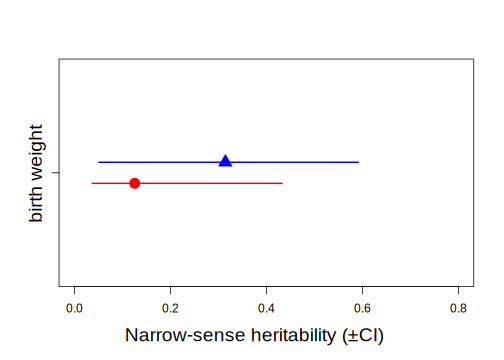
\includegraphics{wam_tuto_files/figure-latex/unnamed-chunk-53-1.pdf}
\caption{\label{fig:unnamed-chunk-53}Female and male heritability of birth weight}
\end{figure}

\hypertarget{modification-of-model-parameter}{%
\subsection{Modification of model parameter}\label{modification-of-model-parameter}}

Unfortunately (to our knowledge), it is not possible to alter the variance matricesand refit them within the model.

\hypertarget{covariance-between-two-random-effects-1}{%
\subsection{Covariance between two random effects}\label{covariance-between-two-random-effects-1}}

Some research questions require to estimate the covariance between two random effects within a univariate model.To do so, we can use the argument \texttt{str}. A similar argument or linking.function \texttt{mm} can be used but it will forced the variance of \texttt{animal} and \texttt{mother} to be equal and the covariance to 1.
As an example, we fit a model which estimate the covariance between the additive genetic variance and the mother variance.
Both variances require to operate on the same level, thus \texttt{animal} and \texttt{mother} require to be associated to the pedigree information.The ginverse list name has to correspond to the first term in the argument or linking.function

\hypertarget{brms-1}{%
\section{brms}\label{brms-1}}

\hypertarget{running-the-model-2}{%
\subsection{Running the model}\label{running-the-model-2}}

First we need to load the \texttt{brms} library:

\begin{Shaded}
\begin{Highlighting}[]
\KeywordTok{library}\NormalTok{(brms)}
\end{Highlighting}
\end{Shaded}

To be able to fit an animal model, \texttt{brms} needs the relativeness (relationship) matrix of the pedigree and not its inverse (as in other softwares).
This can be estimated using the \texttt{nadiv} package created by Pr. Matthew Wolak (\url{https://cran.r-project.org/web/packages/nadiv/index.html}).

\begin{Shaded}
\begin{Highlighting}[]
\NormalTok{Amat \textless{}{-}}\StringTok{ }\KeywordTok{as.matrix}\NormalTok{(nadiv}\OperatorTok{::}\KeywordTok{makeA}\NormalTok{(gryphonped))}
\end{Highlighting}
\end{Shaded}

We are now ready to specify our first model:
The structure of a \texttt{bmrs} model is similar to \texttt{lme4}, thus the random effect is added to the model with the term \texttt{(1\ \textbar{}\ gr(animal,\ cov\ =\ Amat)} which associate the id animal to the matrix of relativeness.
In addition to the synthase of \texttt{lme4}, we includes other features or parameters within the models such as \texttt{chain} which represent the number of Markov chains (defaults to 4), \texttt{core} which represents the number of cores to use when executing the chains in parallel and \texttt{iter} which represents the number of total iterations per chain. For more parameters such as \texttt{thin} or \texttt{warmup/burnin}, you can read the Cran R page of the package (\url{https://cran.r-project.org/web/packages/brms/brms.pdf})

\texttt{bmrs} is a Bayesian Multilevel Models using Stan, doing so we can apply a prior to the model to better shape the distribution of the different variances estimated by the model.
Given that \texttt{bmrs} fit the model using a Bayesian approach via the software \texttt{stan}, we need to specify priors for the model.
Default priors in \texttt{brms} work relatively well, however we strongly suggest to carefully select an adequate prior for your analysis.
In this tutorial we will use the default priors.
To get the prior used by default, we can use the \texttt{get\_prior()} function.

\begin{Shaded}
\begin{Highlighting}[]
\NormalTok{brms\_m1}\FloatTok{.1}\NormalTok{ \textless{}{-}}\StringTok{ }\KeywordTok{brm}\NormalTok{(}
\NormalTok{  bwt }\OperatorTok{\textasciitilde{}}\StringTok{ }\DecValTok{1} \OperatorTok{+}\StringTok{ }\NormalTok{(}\DecValTok{1} \OperatorTok{|}\StringTok{ }\KeywordTok{gr}\NormalTok{(animal, }\DataTypeTok{cov =}\NormalTok{ Amat)),}
  \DataTypeTok{data =}\NormalTok{ gryphon,}
  \DataTypeTok{data2 =} \KeywordTok{list}\NormalTok{(}\DataTypeTok{Amat =}\NormalTok{ Amat),}
  \DataTypeTok{family =} \KeywordTok{gaussian}\NormalTok{(),}
  \DataTypeTok{chains =} \DecValTok{1}\NormalTok{, }\DataTypeTok{cores =} \DecValTok{1}\NormalTok{, }\DataTypeTok{iter =} \DecValTok{100}
\NormalTok{)}

\KeywordTok{save}\NormalTok{(brms\_m1}\FloatTok{.1}\NormalTok{, }\DataTypeTok{file =} \StringTok{"data/brms\_m1\_1.rda"}\NormalTok{)}
\end{Highlighting}
\end{Shaded}

The result of the long model calculation is save in a spare file \texttt{brms\_m1\_1.rda"}. To help readers, we can directly reloading it.
Two distinct plot can be produce to produce some diagnostics graphs \texttt{mcmc\_plot}.Note, that \texttt{sigma} represents the residual standard deviation.

Next,we examine (or directly using the model) the variance estimate and their distributions (via \texttt{summary} or plot).

\begin{Shaded}
\begin{Highlighting}[]
\KeywordTok{load}\NormalTok{(}\StringTok{"data/brms\_m1\_1.rda"}\NormalTok{)}
\KeywordTok{plot}\NormalTok{(brms\_m1}\FloatTok{.1}\NormalTok{)}
\end{Highlighting}
\end{Shaded}

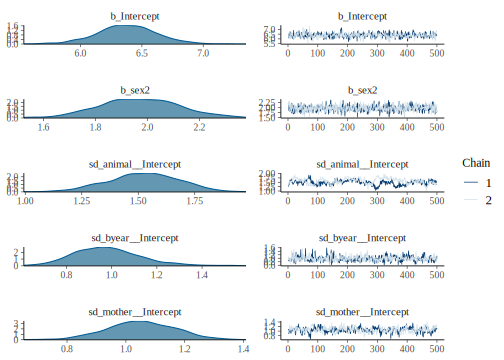
\includegraphics{wam_tuto_files/figure-latex/unnamed-chunk-58-1.pdf}

\begin{Shaded}
\begin{Highlighting}[]
\KeywordTok{mcmc\_plot}\NormalTok{(brms\_m1}\FloatTok{.1}\NormalTok{, }\DataTypeTok{type =} \StringTok{"acf"}\NormalTok{)}
\end{Highlighting}
\end{Shaded}

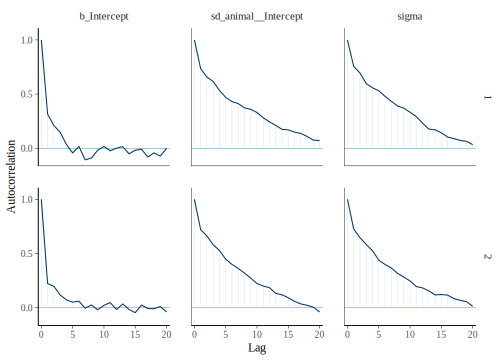
\includegraphics{wam_tuto_files/figure-latex/unnamed-chunk-58-2.pdf}

\begin{Shaded}
\begin{Highlighting}[]
\KeywordTok{summary}\NormalTok{(brms\_m1}\FloatTok{.1}\NormalTok{)}
\end{Highlighting}
\end{Shaded}

\begin{verbatim}
##  Family: gaussian 
##   Links: mu = identity; sigma = identity 
## Formula: bwt ~ 1 + (1 | gr(animal, cov = Amat)) 
##    Data: gryphon (Number of observations: 854) 
##   Draws: 2 chains, each with iter = 1000; warmup = 500; thin = 1;
##          total post-warmup draws = 1000
## 
## Group-Level Effects: 
## ~animal (Number of levels: 854) 
##               Estimate Est.Error l-95% CI u-95% CI Rhat Bulk_ESS Tail_ESS
## sd(Intercept)     1.88      0.17     1.54     2.23 1.03       74       99
## 
## Population-Level Effects: 
##           Estimate Est.Error l-95% CI u-95% CI Rhat Bulk_ESS Tail_ESS
## Intercept     7.60      0.14     7.33     7.86 1.01      428      727
## 
## Family Specific Parameters: 
##       Estimate Est.Error l-95% CI u-95% CI Rhat Bulk_ESS Tail_ESS
## sigma     1.93      0.13     1.66     2.18 1.04       71      112
## 
## Draws were sampled using sampling(NUTS). For each parameter, Bulk_ESS
## and Tail_ESS are effective sample size measures, and Rhat is the potential
## scale reduction factor on split chains (at convergence, Rhat = 1).
\end{verbatim}

The \texttt{plot} of variance showed that the different variances have an normal distribution, the autocorrelation plot or `acf' show that the autocorrelation is close to 0.
The \texttt{summary} exposes the mean (Estimate) of each variance or fixed effect (here just the intercept) associated to their posterior distribution with standard deviation (Est.Error) and two-sided 95\% Credible intervals.
\texttt{Rhat} provides information on the estimate convergence. If it's greater than 1, the chains have not yet converged and it will be require to run more iterations and/or set stronger priors.
\texttt{ESS} represents the Effective sample values as the number of independent samples from the posterior distribution.
However, for the purpose of this guide, the Rhat values are acceptable.

It is also possible to calculate the heritability using the function `as.mcmc'

\begin{Shaded}
\begin{Highlighting}[]
\NormalTok{v\_animal \textless{}{-}}\StringTok{ }\NormalTok{(}\KeywordTok{VarCorr}\NormalTok{(brms\_m1}\FloatTok{.1}\NormalTok{, }\DataTypeTok{summary =} \OtherTok{FALSE}\NormalTok{)}\OperatorTok{$}\NormalTok{animal}\OperatorTok{$}\NormalTok{sd)}\OperatorTok{\^{}}\DecValTok{2}
\NormalTok{v\_r \textless{}{-}}\StringTok{ }\NormalTok{(}\KeywordTok{VarCorr}\NormalTok{(brms\_m1}\FloatTok{.1}\NormalTok{, }\DataTypeTok{summary =} \OtherTok{FALSE}\NormalTok{)}\OperatorTok{$}\NormalTok{residual}\OperatorTok{$}\NormalTok{sd)}\OperatorTok{\^{}}\DecValTok{2}
\NormalTok{h.bwt}\FloatTok{.1}\NormalTok{ \textless{}{-}}\StringTok{ }\KeywordTok{as.mcmc}\NormalTok{(v\_animal }\OperatorTok{/}\StringTok{ }\NormalTok{(v\_animal }\OperatorTok{+}\StringTok{ }\NormalTok{v\_r))}
\KeywordTok{summary}\NormalTok{(h.bwt}\FloatTok{.1}\NormalTok{)}
\end{Highlighting}
\end{Shaded}

\begin{verbatim}
## 
## Iterations = 1:1000
## Thinning interval = 1 
## Number of chains = 1 
## Sample size per chain = 1000 
## 
## 1. Empirical mean and standard deviation for each variable,
##    plus standard error of the mean:
## 
##           Mean             SD       Naive SE Time-series SE 
##       0.484221       0.074533       0.002357       0.009275 
## 
## 2. Quantiles for each variable:
## 
##   2.5%    25%    50%    75%  97.5% 
## 0.3433 0.4338 0.4841 0.5350 0.6369
\end{verbatim}

\begin{Shaded}
\begin{Highlighting}[]
\KeywordTok{plot}\NormalTok{(h.bwt}\FloatTok{.1}\NormalTok{)}
\end{Highlighting}
\end{Shaded}

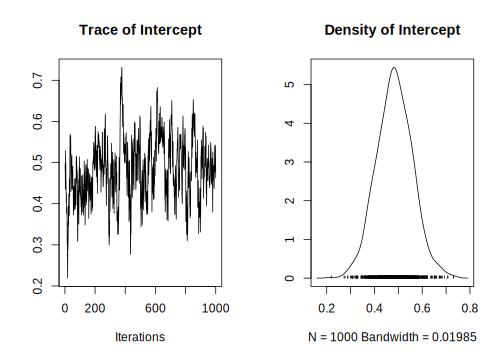
\includegraphics{wam_tuto_files/figure-latex/unnamed-chunk-59-1.pdf}

\begin{Shaded}
\begin{Highlighting}[]
\CommentTok{\# or}
\NormalTok{Var.table \textless{}{-}}\StringTok{ }\KeywordTok{as\_draws\_df}\NormalTok{(brms\_m1}\FloatTok{.1}\NormalTok{)}
\NormalTok{Var.table}\OperatorTok{$}\NormalTok{h.bwt}\FloatTok{.1}\NormalTok{ \textless{}{-}}\StringTok{ }\KeywordTok{as.mcmc}\NormalTok{((Var.table}\OperatorTok{$}\NormalTok{sd\_animal\_\_Intercept)}\OperatorTok{\^{}}\DecValTok{2} \OperatorTok{/}\StringTok{ }\NormalTok{((Var.table}\OperatorTok{$}\NormalTok{sd\_animal\_\_Intercept)}\OperatorTok{\^{}}\DecValTok{2} \OperatorTok{+}\StringTok{ }\NormalTok{(Var.table}\OperatorTok{$}\NormalTok{sigma)}\OperatorTok{\^{}}\DecValTok{2}\NormalTok{))}
\KeywordTok{summary}\NormalTok{(Var.table}\OperatorTok{$}\NormalTok{h.bwt}\FloatTok{.1}\NormalTok{)}
\end{Highlighting}
\end{Shaded}

\begin{verbatim}
## 
## Iterations = 1:1000
## Thinning interval = 1 
## Number of chains = 1 
## Sample size per chain = 1000 
## 
## 1. Empirical mean and standard deviation for each variable,
##    plus standard error of the mean:
## 
##           Mean             SD       Naive SE Time-series SE 
##       0.484221       0.074533       0.002357       0.009275 
## 
## 2. Quantiles for each variable:
## 
##   2.5%    25%    50%    75%  97.5% 
## 0.3433 0.4338 0.4841 0.5350 0.6369
\end{verbatim}

\begin{Shaded}
\begin{Highlighting}[]
\KeywordTok{plot}\NormalTok{(Var.table}\OperatorTok{$}\NormalTok{h.bwt}\FloatTok{.1}\NormalTok{)}
\end{Highlighting}
\end{Shaded}

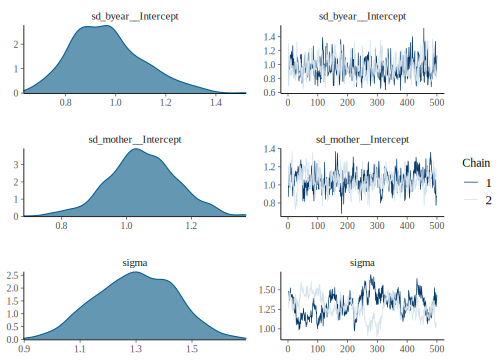
\includegraphics{wam_tuto_files/figure-latex/unnamed-chunk-59-2.pdf}

\hypertarget{adding-fixed-effects-2}{%
\subsection{Adding fixed effects}\label{adding-fixed-effects-2}}

To add effects to a univariate model, we simply modify the priors and the fixed effect portion of the model specification:

\begin{Shaded}
\begin{Highlighting}[]
\NormalTok{brms\_m1}\FloatTok{.2}\NormalTok{ \textless{}{-}}\StringTok{ }\KeywordTok{brm}\NormalTok{(}
\NormalTok{  bwt }\OperatorTok{\textasciitilde{}}\StringTok{ }\DecValTok{1} \OperatorTok{+}\StringTok{ }\NormalTok{sex }\OperatorTok{+}\StringTok{ }\NormalTok{(}\DecValTok{1} \OperatorTok{|}\StringTok{ }\KeywordTok{gr}\NormalTok{(animal, }\DataTypeTok{cov =}\NormalTok{ Amat)),}
  \DataTypeTok{data =}\NormalTok{ gryphon,}
  \DataTypeTok{data2 =} \KeywordTok{list}\NormalTok{(}\DataTypeTok{Amat =}\NormalTok{ Amat),}
  \DataTypeTok{family =} \KeywordTok{gaussian}\NormalTok{(),}
  \DataTypeTok{chains =} \DecValTok{2}\NormalTok{, }\DataTypeTok{cores =} \DecValTok{2}\NormalTok{, }\DataTypeTok{iter =} \DecValTok{1000}
\NormalTok{)}

\KeywordTok{save}\NormalTok{(brms\_m1}\FloatTok{.2}\NormalTok{, }\DataTypeTok{file =} \StringTok{"data/brms\_m1\_2.rda"}\NormalTok{)}
\end{Highlighting}
\end{Shaded}

To save time, the results of the calculation is stored in the spare file \texttt{brms\_m1\_2.rda"}.
We can assess the significance of \texttt{sex} as a fixed effect by examining its posterior distribution.

\begin{Shaded}
\begin{Highlighting}[]
\KeywordTok{load}\NormalTok{(}\StringTok{"data/brms\_m1\_2.rda"}\NormalTok{)}
\KeywordTok{summary}\NormalTok{(brms\_m1}\FloatTok{.2}\NormalTok{)}
\end{Highlighting}
\end{Shaded}

\begin{verbatim}
## Warning: Parts of the model have not converged (some Rhats are > 1.05). Be
## careful when analysing the results! We recommend running more iterations and/or
## setting stronger priors.
\end{verbatim}

\begin{verbatim}
##  Family: gaussian 
##   Links: mu = identity; sigma = identity 
## Formula: bwt ~ 1 + sex + (1 | gr(animal, cov = Amat)) 
##    Data: gryphon (Number of observations: 854) 
##   Draws: 2 chains, each with iter = 1000; warmup = 500; thin = 1;
##          total post-warmup draws = 1000
## 
## Group-Level Effects: 
## ~animal (Number of levels: 854) 
##               Estimate Est.Error l-95% CI u-95% CI Rhat Bulk_ESS Tail_ESS
## sd(Intercept)     1.75      0.16     1.42     2.05 1.13       13      113
## 
## Population-Level Effects: 
##           Estimate Est.Error l-95% CI u-95% CI Rhat Bulk_ESS Tail_ESS
## Intercept     6.06      0.17     5.74     6.41 1.00      358      574
## sex2          2.21      0.16     1.90     2.52 1.00      723      657
## 
## Family Specific Parameters: 
##       Estimate Est.Error l-95% CI u-95% CI Rhat Bulk_ESS Tail_ESS
## sigma     1.71      0.13     1.47     1.98 1.12       14       97
## 
## Draws were sampled using sampling(NUTS). For each parameter, Bulk_ESS
## and Tail_ESS are effective sample size measures, and Rhat is the potential
## scale reduction factor on split chains (at convergence, Rhat = 1).
\end{verbatim}

\begin{Shaded}
\begin{Highlighting}[]
\KeywordTok{plot}\NormalTok{(brms\_m1}\FloatTok{.2}\NormalTok{)}
\end{Highlighting}
\end{Shaded}

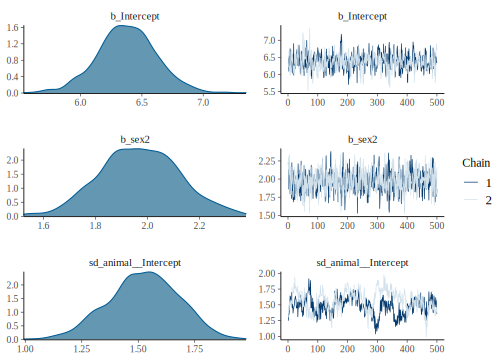
\includegraphics{wam_tuto_files/figure-latex/unnamed-chunk-61-1.pdf}

\begin{Shaded}
\begin{Highlighting}[]
\KeywordTok{mcmc\_plot}\NormalTok{(brms\_m1}\FloatTok{.2}\NormalTok{, }\DataTypeTok{type =} \StringTok{"pairs"}\NormalTok{)}
\end{Highlighting}
\end{Shaded}

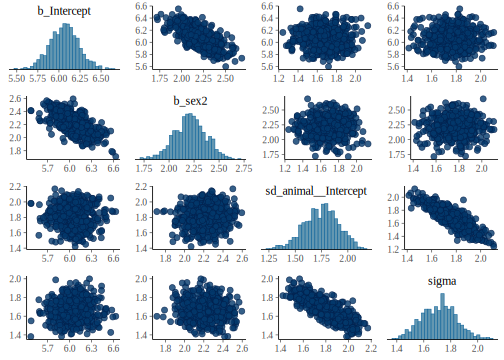
\includegraphics{wam_tuto_files/figure-latex/unnamed-chunk-61-2.pdf}

\begin{Shaded}
\begin{Highlighting}[]
\KeywordTok{summary}\NormalTok{(brms\_m1}\FloatTok{.2}\NormalTok{)}\OperatorTok{$}\NormalTok{fixed}
\end{Highlighting}
\end{Shaded}

\begin{verbatim}
## Warning: Parts of the model have not converged (some Rhats are > 1.05). Be
## careful when analysing the results! We recommend running more iterations and/or
## setting stronger priors.
\end{verbatim}

\begin{verbatim}
##           Estimate Est.Error l-95% CI u-95% CI     Rhat Bulk_ESS Tail_ESS
## Intercept 6.064853 0.1726459 5.735170 6.410117 1.002990 357.5666 574.2620
## sex2      2.210675 0.1574542 1.898645 2.520026 1.002313 722.8016 657.2121
\end{verbatim}

\begin{Shaded}
\begin{Highlighting}[]
\KeywordTok{summary}\NormalTok{(brms\_m1}\FloatTok{.2}\NormalTok{)}\OperatorTok{$}\NormalTok{random}
\end{Highlighting}
\end{Shaded}

\begin{verbatim}
## Warning: Parts of the model have not converged (some Rhats are > 1.05). Be
## careful when analysing the results! We recommend running more iterations and/or
## setting stronger priors.
\end{verbatim}

\begin{verbatim}
## $animal
##               Estimate Est.Error l-95% CI u-95% CI     Rhat Bulk_ESS Tail_ESS
## sd(Intercept) 1.747083 0.1632548 1.419377 2.050884 1.126639 13.10221 113.2445
\end{verbatim}

The posterior distribution of the \texttt{sex2} term does not overlap zero. Thus, we can infer that sex has an effect on birth weight (presence of a sexual dimorphism) in this model and is a useful addition to the model, for most purposes. It is also worth noting that the variance components have changed slightly:

\begin{Shaded}
\begin{Highlighting}[]
\KeywordTok{summary}\NormalTok{(brms\_m1}\FloatTok{.2}\NormalTok{)}\OperatorTok{$}\NormalTok{random}
\end{Highlighting}
\end{Shaded}

\begin{verbatim}
## Warning: Parts of the model have not converged (some Rhats are > 1.05). Be
## careful when analysing the results! We recommend running more iterations and/or
## setting stronger priors.
\end{verbatim}

\begin{verbatim}
## $animal
##               Estimate Est.Error l-95% CI u-95% CI     Rhat Bulk_ESS Tail_ESS
## sd(Intercept) 1.747083 0.1632548 1.419377 2.050884 1.126639 13.10221 113.2445
\end{verbatim}

In fact since sex effects were previously contributing to the residual variance of the model our estimate of \(V_R\) (denoted 'units' in the output) is now slightly lower than before. This has an important consequence for estimating heritability since if we calculate \(V_P\) as \(V_A +V_R\) then as we include fixed effects we will soak up more residual variance driving \(V_P\) . Assuming that \(V_A\) is more or less unaffected by the fixed effects fitted then as \(V_P\) goes down we expect our estimate of \(h^2\) will go up.

\begin{Shaded}
\begin{Highlighting}[]
\NormalTok{v\_animal \textless{}{-}}\StringTok{ }\NormalTok{(}\KeywordTok{VarCorr}\NormalTok{(brms\_m1}\FloatTok{.2}\NormalTok{, }\DataTypeTok{summary =} \OtherTok{FALSE}\NormalTok{)}\OperatorTok{$}\NormalTok{animal}\OperatorTok{$}\NormalTok{sd)}\OperatorTok{\^{}}\DecValTok{2}
\NormalTok{v\_r \textless{}{-}}\StringTok{ }\NormalTok{(}\KeywordTok{VarCorr}\NormalTok{(brms\_m1}\FloatTok{.2}\NormalTok{, }\DataTypeTok{summary =} \OtherTok{FALSE}\NormalTok{)}\OperatorTok{$}\NormalTok{residual}\OperatorTok{$}\NormalTok{sd)}\OperatorTok{\^{}}\DecValTok{2}
\NormalTok{h.bwt}\FloatTok{.2}\NormalTok{ \textless{}{-}}\StringTok{ }\KeywordTok{as.mcmc}\NormalTok{(v\_animal }\OperatorTok{/}\StringTok{ }\NormalTok{(v\_animal }\OperatorTok{+}\StringTok{ }\NormalTok{v\_r))}

\KeywordTok{summary}\NormalTok{(h.bwt}\FloatTok{.2}\NormalTok{)}
\end{Highlighting}
\end{Shaded}

\begin{verbatim}
## 
## Iterations = 1:1000
## Thinning interval = 1 
## Number of chains = 1 
## Sample size per chain = 1000 
## 
## 1. Empirical mean and standard deviation for each variable,
##    plus standard error of the mean:
## 
##           Mean             SD       Naive SE Time-series SE 
##       0.508677       0.080357       0.002541       0.011998 
## 
## 2. Quantiles for each variable:
## 
##   2.5%    25%    50%    75%  97.5% 
## 0.3427 0.4549 0.5107 0.5675 0.6576
\end{verbatim}

\begin{Shaded}
\begin{Highlighting}[]
\KeywordTok{summary}\NormalTok{(h.bwt}\FloatTok{.1}\NormalTok{)}
\end{Highlighting}
\end{Shaded}

\begin{verbatim}
## 
## Iterations = 1:1000
## Thinning interval = 1 
## Number of chains = 1 
## Sample size per chain = 1000 
## 
## 1. Empirical mean and standard deviation for each variable,
##    plus standard error of the mean:
## 
##           Mean             SD       Naive SE Time-series SE 
##       0.484221       0.074533       0.002357       0.009275 
## 
## 2. Quantiles for each variable:
## 
##   2.5%    25%    50%    75%  97.5% 
## 0.3433 0.4338 0.4841 0.5350 0.6369
\end{verbatim}

Here \(h^2\) has increased slightly from 0.5010 to 0.4192 (again, your values may differ slightly due to Monte Carlo error). Which is the better estimate?
It depends on what your question is. The first is an estimate of the proportion of variance in birth weight explained by additive effects, the latter is an estimate of the proportion of variance in birth weight after conditioning on sex that is explained by additive effects.
An important piece of advice, each researcher should be consistent in how they name their estimates and always correctly describe which estimates they are using conditional or not (to avoid any confusion).

\hypertarget{adding-random-effects-2}{%
\subsection{Adding random effects}\label{adding-random-effects-2}}

This is done by simply modifying the model statement in the same way, but requires addition of a prior for the new random effect. For instance, we can fit an effect of birth year:

\begin{Shaded}
\begin{Highlighting}[]
\NormalTok{brms\_m1}\FloatTok{.3}\NormalTok{ \textless{}{-}}\StringTok{ }\KeywordTok{brm}\NormalTok{(}
\NormalTok{  bwt }\OperatorTok{\textasciitilde{}}\StringTok{ }\DecValTok{1} \OperatorTok{+}\StringTok{ }\NormalTok{sex }\OperatorTok{+}\StringTok{ }\NormalTok{(}\DecValTok{1} \OperatorTok{|}\StringTok{ }\KeywordTok{gr}\NormalTok{(animal, }\DataTypeTok{cov =}\NormalTok{ Amat)) }\OperatorTok{+}\StringTok{ }\NormalTok{(}\DecValTok{1} \OperatorTok{|}\StringTok{ }\NormalTok{byear) }\OperatorTok{+}\StringTok{ }\NormalTok{(}\DecValTok{1} \OperatorTok{|}\StringTok{ }\NormalTok{mother),}
  \DataTypeTok{data =}\NormalTok{ gryphon,}
  \DataTypeTok{data2 =} \KeywordTok{list}\NormalTok{(}\DataTypeTok{Amat =}\NormalTok{ Amat),}
  \DataTypeTok{family =} \KeywordTok{gaussian}\NormalTok{(),}
  \DataTypeTok{chains =} \DecValTok{2}\NormalTok{, }\DataTypeTok{cores =} \DecValTok{2}\NormalTok{, }\DataTypeTok{iter =} \DecValTok{1000}
\NormalTok{)}

\KeywordTok{save}\NormalTok{(brms\_m1}\FloatTok{.3}\NormalTok{, }\DataTypeTok{file =} \StringTok{"data/brms\_m1\_3.rda"}\NormalTok{)}
\end{Highlighting}
\end{Shaded}

To save time, the results of the calculation is stored in the spare file \texttt{brms\_m1\_3.rda"}.
We can assess the significance of \texttt{sex} as a fixed effect by examining its posterior distribution.

\begin{Shaded}
\begin{Highlighting}[]
\KeywordTok{load}\NormalTok{(}\StringTok{"data/brms\_m1\_3.rda"}\NormalTok{)}

\KeywordTok{plot}\NormalTok{(brms\_m1}\FloatTok{.3}\NormalTok{, }\DataTypeTok{ask =} \OtherTok{FALSE}\NormalTok{, }\DataTypeTok{N =} \DecValTok{3}\NormalTok{)}
\end{Highlighting}
\end{Shaded}

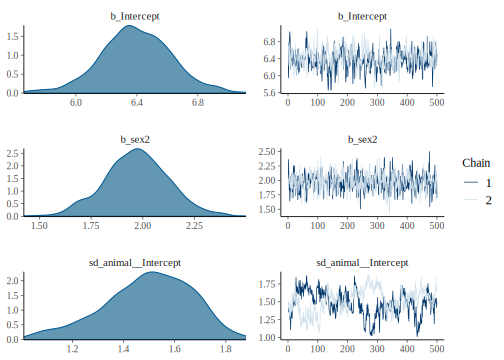
\includegraphics{wam_tuto_files/figure-latex/unnamed-chunk-65-1.pdf} 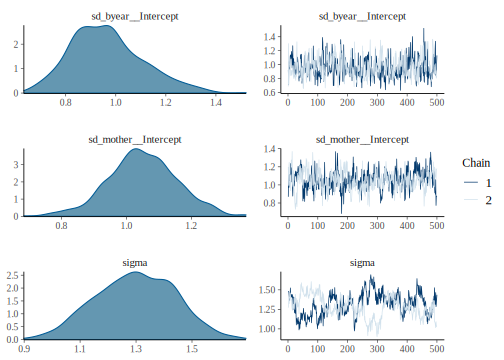
\includegraphics{wam_tuto_files/figure-latex/unnamed-chunk-65-2.pdf}

\begin{Shaded}
\begin{Highlighting}[]
\KeywordTok{summary}\NormalTok{(brms\_m1}\FloatTok{.3}\NormalTok{)}\OperatorTok{$}\NormalTok{random}
\end{Highlighting}
\end{Shaded}

\begin{verbatim}
## Warning: Parts of the model have not converged (some Rhats are > 1.05). Be
## careful when analysing the results! We recommend running more iterations and/or
## setting stronger priors.
\end{verbatim}

\begin{verbatim}
## $animal
##               Estimate Est.Error l-95% CI u-95% CI     Rhat Bulk_ESS Tail_ESS
## sd(Intercept) 1.496464 0.1708587 1.105797 1.782062 1.163193 9.153202 50.78299
## 
## $byear
##                Estimate Est.Error  l-95% CI u-95% CI     Rhat Bulk_ESS Tail_ESS
## sd(Intercept) 0.9642702  0.144174 0.7147103 1.280642 1.002215 399.5806 642.4663
## 
## $mother
##               Estimate Est.Error  l-95% CI u-95% CI     Rhat Bulk_ESS Tail_ESS
## sd(Intercept) 1.050225 0.1057319 0.8292744 1.258439 1.011062 192.6606 379.2063
\end{verbatim}

Here partitioning of significant birth year and maternal variance has resulted in a further decrease in \(V_R\) but also a decrease in \(V_A\). The latter is because maternal effects of the sort we simulated (fixed differences between mothers) will have the consequence of increasing similarity among maternal siblings. Consequently they can look very much like an additive genetic effects and if present, but unmodelled, represent a type of `common environment effect' that can - and will- cause upward bias in \(V_A\) and so \(h^2\). Let's compare the estimates of heritability from each of models 1.2, 1.3 and 1.4:

\begin{Shaded}
\begin{Highlighting}[]
\NormalTok{v\_animal \textless{}{-}}\StringTok{ }\NormalTok{(}\KeywordTok{VarCorr}\NormalTok{(brms\_m1}\FloatTok{.3}\NormalTok{, }\DataTypeTok{summary =} \OtherTok{FALSE}\NormalTok{)}\OperatorTok{$}\NormalTok{animal}\OperatorTok{$}\NormalTok{sd)}\OperatorTok{\^{}}\DecValTok{2}
\NormalTok{v\_byear \textless{}{-}}\StringTok{ }\NormalTok{(}\KeywordTok{VarCorr}\NormalTok{(brms\_m1}\FloatTok{.3}\NormalTok{, }\DataTypeTok{summary =} \OtherTok{FALSE}\NormalTok{)}\OperatorTok{$}\NormalTok{byear}\OperatorTok{$}\NormalTok{sd)}\OperatorTok{\^{}}\DecValTok{2}
\NormalTok{v\_mother \textless{}{-}}\StringTok{ }\NormalTok{(}\KeywordTok{VarCorr}\NormalTok{(brms\_m1}\FloatTok{.3}\NormalTok{, }\DataTypeTok{summary =} \OtherTok{FALSE}\NormalTok{)}\OperatorTok{$}\NormalTok{mother}\OperatorTok{$}\NormalTok{sd)}\OperatorTok{\^{}}\DecValTok{2}
\NormalTok{v\_r \textless{}{-}}\StringTok{ }\NormalTok{(}\KeywordTok{VarCorr}\NormalTok{(brms\_m1}\FloatTok{.3}\NormalTok{, }\DataTypeTok{summary =} \OtherTok{FALSE}\NormalTok{)}\OperatorTok{$}\NormalTok{residual}\OperatorTok{$}\NormalTok{sd)}\OperatorTok{\^{}}\DecValTok{2}
\NormalTok{h.bwt}\FloatTok{.3}\NormalTok{ \textless{}{-}}\StringTok{ }\KeywordTok{as.mcmc}\NormalTok{(v\_animal }\OperatorTok{/}\StringTok{ }\NormalTok{(v\_animal }\OperatorTok{+}\StringTok{ }\NormalTok{v\_byear }\OperatorTok{+}\StringTok{ }\NormalTok{v\_mother }\OperatorTok{+}\StringTok{ }\NormalTok{v\_r))}
\KeywordTok{summary}\NormalTok{(h.bwt}\FloatTok{.3}\NormalTok{)}
\end{Highlighting}
\end{Shaded}

\begin{verbatim}
## 
## Iterations = 1:1000
## Thinning interval = 1 
## Number of chains = 1 
## Sample size per chain = 1000 
## 
## 1. Empirical mean and standard deviation for each variable,
##    plus standard error of the mean:
## 
##           Mean             SD       Naive SE Time-series SE 
##       0.375509       0.078767       0.002491       0.012711 
## 
## 2. Quantiles for each variable:
## 
##   2.5%    25%    50%    75%  97.5% 
## 0.2140 0.3240 0.3764 0.4322 0.5182
\end{verbatim}

\begin{Shaded}
\begin{Highlighting}[]
\KeywordTok{summary}\NormalTok{(h.bwt}\FloatTok{.2}\NormalTok{)}
\end{Highlighting}
\end{Shaded}

\begin{verbatim}
## 
## Iterations = 1:1000
## Thinning interval = 1 
## Number of chains = 1 
## Sample size per chain = 1000 
## 
## 1. Empirical mean and standard deviation for each variable,
##    plus standard error of the mean:
## 
##           Mean             SD       Naive SE Time-series SE 
##       0.508677       0.080357       0.002541       0.011998 
## 
## 2. Quantiles for each variable:
## 
##   2.5%    25%    50%    75%  97.5% 
## 0.3427 0.4549 0.5107 0.5675 0.6576
\end{verbatim}

\begin{Shaded}
\begin{Highlighting}[]
\KeywordTok{summary}\NormalTok{(h.bwt}\FloatTok{.1}\NormalTok{)}
\end{Highlighting}
\end{Shaded}

\begin{verbatim}
## 
## Iterations = 1:1000
## Thinning interval = 1 
## Number of chains = 1 
## Sample size per chain = 1000 
## 
## 1. Empirical mean and standard deviation for each variable,
##    plus standard error of the mean:
## 
##           Mean             SD       Naive SE Time-series SE 
##       0.484221       0.074533       0.002357       0.009275 
## 
## 2. Quantiles for each variable:
## 
##   2.5%    25%    50%    75%  97.5% 
## 0.3433 0.4338 0.4841 0.5350 0.6369
\end{verbatim}

\begin{Shaded}
\begin{Highlighting}[]
\CommentTok{\# or}
\NormalTok{Var.table \textless{}{-}}\StringTok{ }\KeywordTok{as\_draws\_df}\NormalTok{(brms\_m1}\FloatTok{.3}\NormalTok{)}
\NormalTok{Var.table}\OperatorTok{$}\NormalTok{h.bwt}\FloatTok{.3}\NormalTok{ \textless{}{-}}\StringTok{ }\KeywordTok{as.mcmc}\NormalTok{((Var.table}\OperatorTok{$}\NormalTok{sd\_animal\_\_Intercept)}\OperatorTok{\^{}}\DecValTok{2} \OperatorTok{/}\StringTok{ }\NormalTok{((Var.table}\OperatorTok{$}\NormalTok{sd\_animal\_\_Intercept)}\OperatorTok{\^{}}\DecValTok{2} \OperatorTok{+}\StringTok{ }\NormalTok{(Var.table}\OperatorTok{$}\NormalTok{sd\_byear\_\_Intercept)}\OperatorTok{\^{}}\DecValTok{2} \OperatorTok{+}\StringTok{ }\NormalTok{(Var.table}\OperatorTok{$}\NormalTok{sd\_mother\_\_Intercept)}\OperatorTok{\^{}}\DecValTok{2} \OperatorTok{+}\StringTok{ }\NormalTok{(Var.table}\OperatorTok{$}\NormalTok{sigma)}\OperatorTok{\^{}}\DecValTok{2}\NormalTok{))}
\KeywordTok{summary}\NormalTok{(Var.table}\OperatorTok{$}\NormalTok{h.bwt}\FloatTok{.3}\NormalTok{)}
\end{Highlighting}
\end{Shaded}

\begin{verbatim}
## 
## Iterations = 1:1000
## Thinning interval = 1 
## Number of chains = 1 
## Sample size per chain = 1000 
## 
## 1. Empirical mean and standard deviation for each variable,
##    plus standard error of the mean:
## 
##           Mean             SD       Naive SE Time-series SE 
##       0.375509       0.078767       0.002491       0.012711 
## 
## 2. Quantiles for each variable:
## 
##   2.5%    25%    50%    75%  97.5% 
## 0.2140 0.3240 0.3764 0.4322 0.5182
\end{verbatim}

\begin{Shaded}
\begin{Highlighting}[]
\KeywordTok{plot}\NormalTok{(Var.table}\OperatorTok{$}\NormalTok{h.bwt}\FloatTok{.3}\NormalTok{)}
\end{Highlighting}
\end{Shaded}

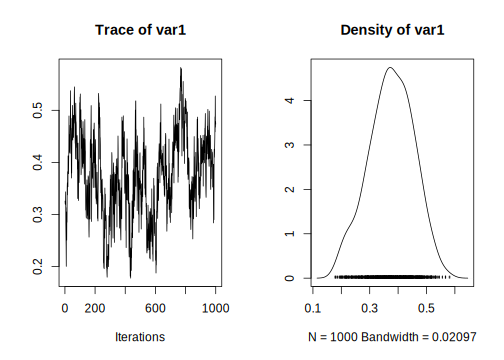
\includegraphics{wam_tuto_files/figure-latex/unnamed-chunk-66-1.pdf}

\hypertarget{testing-significance-of-variance-components-1}{%
\subsection{Testing significance of variance components}\label{testing-significance-of-variance-components-1}}

While testing the significance of fixed effects by evaluating whether or not their posterior distributions overlap zero was simple and valid, this approach does not work for variance components.
Variance components are bounded to be positive (given a proper prior), and thus even when a random effect is not meaningful, its posterior distribution will never overlap zero.

Model comparisons can be performed using the function \texttt{loo\_compare} using \texttt{waic} or weighted AIC.

\begin{Shaded}
\begin{Highlighting}[]
\NormalTok{brms\_m1}\FloatTok{.3}\NormalTok{ \textless{}{-}}\StringTok{ }\KeywordTok{add\_criterion}\NormalTok{(brms\_m1}\FloatTok{.3}\NormalTok{, }\StringTok{"waic"}\NormalTok{)}
\end{Highlighting}
\end{Shaded}

\begin{verbatim}
## Warning: 
## 311 (36.4%) p_waic estimates greater than 0.4. We recommend trying loo instead.
\end{verbatim}

\begin{Shaded}
\begin{Highlighting}[]
\NormalTok{brms\_m1}\FloatTok{.1}\NormalTok{ \textless{}{-}}\StringTok{ }\KeywordTok{add\_criterion}\NormalTok{(brms\_m1}\FloatTok{.1}\NormalTok{, }\StringTok{"waic"}\NormalTok{)}
\end{Highlighting}
\end{Shaded}

\begin{verbatim}
## Warning: 
## 236 (27.6%) p_waic estimates greater than 0.4. We recommend trying loo instead.
\end{verbatim}

\begin{Shaded}
\begin{Highlighting}[]
\KeywordTok{loo\_compare}\NormalTok{(brms\_m1}\FloatTok{.3}\NormalTok{, brms\_m1}\FloatTok{.1}\NormalTok{, }\DataTypeTok{criterion =} \StringTok{"waic"}\NormalTok{)}
\end{Highlighting}
\end{Shaded}

\begin{verbatim}
##           elpd_diff se_diff
## brms_m1.3    0.0       0.0 
## brms_m1.1 -282.7      14.0
\end{verbatim}

\hypertarget{further-partitioning-of-the-variance}{%
\subsection{Further partitioning of the variance}\label{further-partitioning-of-the-variance}}

Depending of the research question and the presence of different group within the dataset, \texttt{brms} allowed to partition the variance at different groups.
Two distinct approch can be done to partition the different random effect: using an extra argument \texttt{by=sex} or by adding \texttt{(0+sex\textbar{})} before the \texttt{\textbar{}}. Notes, here we used \texttt{\textbar{}\textbar{}} which not estimate a possible covariance between groups (female and male) for the random effect.

\begin{Shaded}
\begin{Highlighting}[]
\NormalTok{brms\_m1}\FloatTok{.4}\NormalTok{ \textless{}{-}}\StringTok{ }\KeywordTok{brm}\NormalTok{(}
  \CommentTok{\#  bwt \textasciitilde{} 1 +  sex + (1 | gr(animal, cov = Amat, by = sex))+ (1 | gr(byear, by = sex)) + (1 | gr(mother, by = sex)),}
\NormalTok{  bwt }\OperatorTok{\textasciitilde{}}\StringTok{ }\DecValTok{1} \OperatorTok{+}\StringTok{ }\NormalTok{sex }\OperatorTok{+}\StringTok{ }\NormalTok{(}\DecValTok{0} \OperatorTok{+}\StringTok{ }\NormalTok{sex }\OperatorTok{||}\StringTok{ }\KeywordTok{gr}\NormalTok{(animal, }\DataTypeTok{cov =}\NormalTok{ Amat)) }\OperatorTok{+}\StringTok{ }\NormalTok{(}\DecValTok{0} \OperatorTok{+}\StringTok{ }\NormalTok{sex }\OperatorTok{||}\StringTok{ }\NormalTok{byear) }\OperatorTok{+}\StringTok{ }\NormalTok{(}\DecValTok{0} \OperatorTok{+}\StringTok{ }\NormalTok{sex }\OperatorTok{||}\StringTok{ }\NormalTok{mother),}
  \DataTypeTok{data =}\NormalTok{ gryphon,}
  \DataTypeTok{data2 =} \KeywordTok{list}\NormalTok{(}\DataTypeTok{Amat =}\NormalTok{ Amat),}
  \DataTypeTok{family =} \KeywordTok{gaussian}\NormalTok{(),}
  \DataTypeTok{chains =} \DecValTok{2}\NormalTok{, }\DataTypeTok{cores =} \DecValTok{2}\NormalTok{, }\DataTypeTok{iter =} \DecValTok{1000}
\NormalTok{)}

\KeywordTok{save}\NormalTok{(brms\_m1}\FloatTok{.4}\NormalTok{, }\DataTypeTok{file =} \StringTok{"data/brms\_m1\_4.rda"}\NormalTok{)}
\end{Highlighting}
\end{Shaded}

To save time, the results of the calculation is stored in the spare file \texttt{brms\_m1\_4.rda"}.

\begin{Shaded}
\begin{Highlighting}[]
\KeywordTok{load}\NormalTok{(}\StringTok{"data/brms\_m1\_4.rda"}\NormalTok{)}
\KeywordTok{summary}\NormalTok{(brms\_m1}\FloatTok{.4}\NormalTok{)}
\end{Highlighting}
\end{Shaded}

\begin{verbatim}
## Warning: Parts of the model have not converged (some Rhats are > 1.05). Be
## careful when analysing the results! We recommend running more iterations and/or
## setting stronger priors.
\end{verbatim}

\begin{verbatim}
##  Family: gaussian 
##   Links: mu = identity; sigma = identity 
## Formula: bwt ~ 1 + sex + (0 + sex || gr(animal, cov = Amat)) + (0 + sex || byear) + (0 + sex || mother) 
##    Data: gryphon (Number of observations: 854) 
##   Draws: 2 chains, each with iter = 1000; warmup = 500; thin = 1;
##          total post-warmup draws = 1000
## 
## Group-Level Effects: 
## ~animal (Number of levels: 854) 
##          Estimate Est.Error l-95% CI u-95% CI Rhat Bulk_ESS Tail_ESS
## sd(sex1)     1.39      0.22     0.88     1.77 1.02       56      116
## sd(sex2)     1.06      0.31     0.35     1.57 1.06       29       63
## 
## ~byear (Number of levels: 34) 
##          Estimate Est.Error l-95% CI u-95% CI Rhat Bulk_ESS Tail_ESS
## sd(sex1)     0.91      0.18     0.61     1.29 1.02      381      542
## sd(sex2)     1.09      0.20     0.77     1.56 1.01      310      626
## 
## ~mother (Number of levels: 394) 
##          Estimate Est.Error l-95% CI u-95% CI Rhat Bulk_ESS Tail_ESS
## sd(sex1)     0.90      0.21     0.47     1.29 1.01      143      219
## sd(sex2)     1.34      0.16     1.00     1.65 1.01      143      396
## 
## Population-Level Effects: 
##           Estimate Est.Error l-95% CI u-95% CI Rhat Bulk_ESS Tail_ESS
## Intercept     6.29      0.24     5.85     6.78 1.01      435      444
## sex2          2.03      0.35     1.31     2.69 1.00      568      679
## 
## Family Specific Parameters: 
##       Estimate Est.Error l-95% CI u-95% CI Rhat Bulk_ESS Tail_ESS
## sigma     1.45      0.16     1.09     1.72 1.05       27       35
## 
## Draws were sampled using sampling(NUTS). For each parameter, Bulk_ESS
## and Tail_ESS are effective sample size measures, and Rhat is the potential
## scale reduction factor on split chains (at convergence, Rhat = 1).
\end{verbatim}

We can see the model estimate variance for both sexes. However, the residual level or sigma is not splitted by sexes. A futher and more complex code need to be performed, thus we can estimate the sex-specific heritability.

\begin{Shaded}
\begin{Highlighting}[]
\NormalTok{bf\_m1}\FloatTok{.5}\NormalTok{ \textless{}{-}}\StringTok{ }\KeywordTok{bf}\NormalTok{(}
\NormalTok{  bwt }\OperatorTok{\textasciitilde{}}\StringTok{ }\DecValTok{1} \OperatorTok{+}\StringTok{ }\NormalTok{sex }\OperatorTok{+}\StringTok{ }\NormalTok{(}\DecValTok{0} \OperatorTok{+}\StringTok{ }\NormalTok{sex }\OperatorTok{||}\StringTok{ }\KeywordTok{gr}\NormalTok{(animal, }\DataTypeTok{cov =}\NormalTok{ Amat)) }\OperatorTok{+}\StringTok{ }\NormalTok{(}\DecValTok{0} \OperatorTok{+}\StringTok{ }\NormalTok{sex }\OperatorTok{||}\StringTok{ }\NormalTok{mother) }\OperatorTok{+}\StringTok{ }\NormalTok{(}\DecValTok{0} \OperatorTok{+}\StringTok{ }\NormalTok{sex }\OperatorTok{||}\StringTok{ }\NormalTok{byear),}
\NormalTok{  sigma }\OperatorTok{\textasciitilde{}}\StringTok{ }\NormalTok{sex }\OperatorTok{{-}}\StringTok{ }\DecValTok{1}
\NormalTok{)}

\NormalTok{brms\_m1}\FloatTok{.5}\NormalTok{ \textless{}{-}}\StringTok{ }\KeywordTok{brm}\NormalTok{(bf\_m1}\FloatTok{.5}\NormalTok{,}
  \DataTypeTok{data =}\NormalTok{ gryphon,}
  \DataTypeTok{data2 =} \KeywordTok{list}\NormalTok{(}\DataTypeTok{Amat =}\NormalTok{ Amat),}
  \DataTypeTok{family =} \KeywordTok{gaussian}\NormalTok{(),}
  \DataTypeTok{chains =} \DecValTok{1}\NormalTok{, }\DataTypeTok{cores =} \DecValTok{1}\NormalTok{, }\DataTypeTok{iter =} \DecValTok{1000}
\NormalTok{)}

\KeywordTok{save}\NormalTok{(brms\_m1}\FloatTok{.5}\NormalTok{, }\DataTypeTok{file =} \StringTok{"data/brms\_m1\_5.rda"}\NormalTok{)}
\end{Highlighting}
\end{Shaded}

To save time, the results of the calculation is stored in the spare file \texttt{brms\_m1\_4.rda"}.

\begin{Shaded}
\begin{Highlighting}[]
\KeywordTok{load}\NormalTok{(}\StringTok{"data/brms\_m1\_5.rda"}\NormalTok{)}
\KeywordTok{summary}\NormalTok{(brms\_m1}\FloatTok{.5}\NormalTok{)}
\end{Highlighting}
\end{Shaded}

\begin{verbatim}
## Warning: Parts of the model have not converged (some Rhats are > 1.05). Be
## careful when analysing the results! We recommend running more iterations and/or
## setting stronger priors.
\end{verbatim}

\begin{verbatim}
##  Family: gaussian 
##   Links: mu = identity; sigma = log 
## Formula: bwt ~ 1 + sex + (0 + sex || gr(animal, cov = Amat)) + (0 + sex || mother) + (0 + sex || byear) 
##          sigma ~ sex - 1
##    Data: gryphon (Number of observations: 854) 
##   Draws: 1 chains, each with iter = 1000; warmup = 500; thin = 1;
##          total post-warmup draws = 500
## 
## Group-Level Effects: 
## ~animal (Number of levels: 854) 
##          Estimate Est.Error l-95% CI u-95% CI Rhat Bulk_ESS Tail_ESS
## sd(sex1)     1.56      0.29     1.02     2.09 1.17        4       30
## sd(sex2)     1.61      0.41     0.52     2.08 1.36        2       21
## 
## ~byear (Number of levels: 34) 
##          Estimate Est.Error l-95% CI u-95% CI Rhat Bulk_ESS Tail_ESS
## sd(sex1)     0.91      0.18     0.59     1.36 1.01      153      229
## sd(sex2)     1.06      0.20     0.75     1.49 1.00      170      143
## 
## ~mother (Number of levels: 394) 
##          Estimate Est.Error l-95% CI u-95% CI Rhat Bulk_ESS Tail_ESS
## sd(sex1)     0.88      0.21     0.41     1.25 1.01       73      134
## sd(sex2)     1.27      0.18     0.88     1.59 1.01       31       64
## 
## Population-Level Effects: 
##            Estimate Est.Error l-95% CI u-95% CI Rhat Bulk_ESS Tail_ESS
## Intercept      6.29      0.23     5.88     6.75 1.00      209      313
## sex2           2.02      0.31     1.49     2.66 1.00      127      296
## sigma_sex1     0.22      0.21    -0.25     0.54 1.15        5       12
## sigma_sex2    -0.20      0.40    -0.82     0.54 1.59        2       15
## 
## Draws were sampled using sampling(NUTS). For each parameter, Bulk_ESS
## and Tail_ESS are effective sample size measures, and Rhat is the potential
## scale reduction factor on split chains (at convergence, Rhat = 1).
\end{verbatim}

\begin{Shaded}
\begin{Highlighting}[]
\CommentTok{\#}
\NormalTok{Var.table \textless{}{-}}\StringTok{ }\KeywordTok{as\_draws\_df}\NormalTok{(brms\_m1}\FloatTok{.5}\NormalTok{)}
\NormalTok{Var.table}\OperatorTok{$}\NormalTok{h.bwt.f \textless{}{-}}\StringTok{ }\KeywordTok{as.mcmc}\NormalTok{((Var.table}\OperatorTok{$}\NormalTok{sd\_animal\_\_sex1)}\OperatorTok{\^{}}\DecValTok{2} \OperatorTok{/}\StringTok{ }\NormalTok{((Var.table}\OperatorTok{$}\NormalTok{sd\_animal\_\_sex1)}\OperatorTok{\^{}}\DecValTok{2} \OperatorTok{+}\StringTok{ }\NormalTok{(Var.table}\OperatorTok{$}\StringTok{ }\NormalTok{sd\_byear\_\_sex1)}\OperatorTok{\^{}}\DecValTok{2} \OperatorTok{+}\StringTok{ }\NormalTok{(Var.table}\OperatorTok{$}\NormalTok{sd\_mother\_\_sex1)}\OperatorTok{\^{}}\DecValTok{2} \OperatorTok{+}\StringTok{ }\NormalTok{(Var.table}\OperatorTok{$}\NormalTok{b\_sigma\_sex1)}\OperatorTok{\^{}}\DecValTok{2}\NormalTok{))}
\NormalTok{Var.table}\OperatorTok{$}\NormalTok{h.bwt.m \textless{}{-}}\StringTok{ }\KeywordTok{as.mcmc}\NormalTok{((Var.table}\OperatorTok{$}\NormalTok{sd\_animal\_\_sex2)}\OperatorTok{\^{}}\DecValTok{2} \OperatorTok{/}\StringTok{ }\NormalTok{((Var.table}\OperatorTok{$}\NormalTok{sd\_animal\_\_sex2)}\OperatorTok{\^{}}\DecValTok{2} \OperatorTok{+}\StringTok{ }\NormalTok{(Var.table}\OperatorTok{$}\StringTok{ }\NormalTok{sd\_byear\_\_sex2)}\OperatorTok{\^{}}\DecValTok{2} \OperatorTok{+}\StringTok{ }\NormalTok{(Var.table}\OperatorTok{$}\NormalTok{sd\_mother\_\_sex2)}\OperatorTok{\^{}}\DecValTok{2} \OperatorTok{+}\StringTok{ }\NormalTok{(Var.table}\OperatorTok{$}\NormalTok{b\_sigma\_sex2)}\OperatorTok{\^{}}\DecValTok{2}\NormalTok{))}
\KeywordTok{summary}\NormalTok{(Var.table}\OperatorTok{$}\NormalTok{h.bwt.f)}
\end{Highlighting}
\end{Shaded}

\begin{verbatim}
## 
## Iterations = 1:500
## Thinning interval = 1 
## Number of chains = 1 
## Sample size per chain = 500 
## 
## 1. Empirical mean and standard deviation for each variable,
##    plus standard error of the mean:
## 
##           Mean             SD       Naive SE Time-series SE 
##       0.575443       0.126621       0.005663       0.031251 
## 
## 2. Quantiles for each variable:
## 
##   2.5%    25%    50%    75%  97.5% 
## 0.3075 0.4863 0.5811 0.6741 0.7800
\end{verbatim}

\begin{Shaded}
\begin{Highlighting}[]
\KeywordTok{summary}\NormalTok{(Var.table}\OperatorTok{$}\NormalTok{h.bwt.m)}
\end{Highlighting}
\end{Shaded}

\begin{verbatim}
## 
## Iterations = 1:500
## Thinning interval = 1 
## Number of chains = 1 
## Sample size per chain = 500 
## 
## 1. Empirical mean and standard deviation for each variable,
##    plus standard error of the mean:
## 
##           Mean             SD       Naive SE Time-series SE 
##       0.463879       0.155395       0.006949       0.078323 
## 
## 2. Quantiles for each variable:
## 
##    2.5%     25%     50%     75%   97.5% 
## 0.06693 0.43668 0.50150 0.55729 0.66016
\end{verbatim}

\begin{Shaded}
\begin{Highlighting}[]
\KeywordTok{plot}\NormalTok{(Var.table}\OperatorTok{$}\NormalTok{h.bwt.f)}
\end{Highlighting}
\end{Shaded}

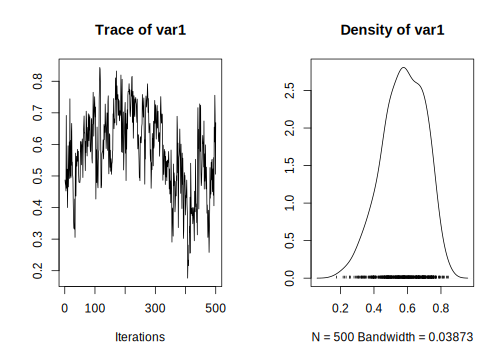
\includegraphics{wam_tuto_files/figure-latex/unnamed-chunk-71-1.pdf}

\begin{Shaded}
\begin{Highlighting}[]
\KeywordTok{plot}\NormalTok{(Var.table}\OperatorTok{$}\NormalTok{h.bwt.m)}
\end{Highlighting}
\end{Shaded}

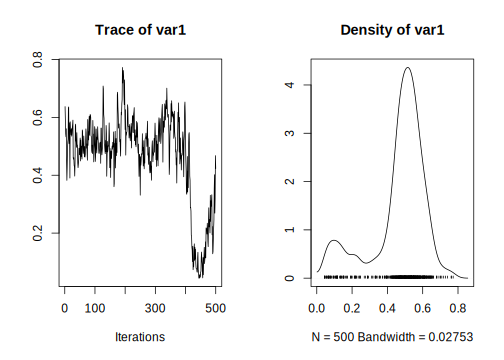
\includegraphics{wam_tuto_files/figure-latex/unnamed-chunk-71-2.pdf}

Here, we can plot the point estimates of the \(h^2\) which seems to differ between sexes, but their CI overlaps.

\begin{Shaded}
\begin{Highlighting}[]
\NormalTok{h2.sex \textless{}{-}}\StringTok{ }\KeywordTok{rbind}\NormalTok{(}
  \KeywordTok{cbind}\NormalTok{(}\KeywordTok{summary}\NormalTok{(Var.table}\OperatorTok{$}\NormalTok{h.bwt.f)}\OperatorTok{$}\NormalTok{statistics[}\DecValTok{1}\NormalTok{], }\KeywordTok{summary}\NormalTok{(Var.table}\OperatorTok{$}\NormalTok{h.bwt.f)}\OperatorTok{$}\NormalTok{quantiles[}\DecValTok{1}\NormalTok{], }\KeywordTok{summary}\NormalTok{(Var.table}\OperatorTok{$}\NormalTok{h.bwt.f)}\OperatorTok{$}\NormalTok{quantiles[}\DecValTok{5}\NormalTok{]),}
  \KeywordTok{cbind}\NormalTok{(}\KeywordTok{summary}\NormalTok{(Var.table}\OperatorTok{$}\NormalTok{h.bwt.m)}\OperatorTok{$}\NormalTok{statistics[}\DecValTok{1}\NormalTok{], }\KeywordTok{summary}\NormalTok{(Var.table}\OperatorTok{$}\NormalTok{h.bwt.m)}\OperatorTok{$}\NormalTok{quantiles[}\DecValTok{1}\NormalTok{], }\KeywordTok{summary}\NormalTok{(Var.table}\OperatorTok{$}\NormalTok{h.bwt.m)}\OperatorTok{$}\NormalTok{quantiles[}\DecValTok{5}\NormalTok{])}
\NormalTok{)}

\KeywordTok{plot}\NormalTok{(}\KeywordTok{c}\NormalTok{(}\FloatTok{0.95}\NormalTok{, }\FloatTok{1.05}\NormalTok{) }\OperatorTok{\textasciitilde{}}\StringTok{ }\NormalTok{h2.sex[, }\DecValTok{1}\NormalTok{], }\DataTypeTok{xlim =} \KeywordTok{c}\NormalTok{(}\DecValTok{0}\NormalTok{, }\FloatTok{0.8}\NormalTok{), }\DataTypeTok{ylim =} \KeywordTok{c}\NormalTok{(}\FloatTok{0.5}\NormalTok{, }\FloatTok{1.5}\NormalTok{), , }\DataTypeTok{xlab =} \StringTok{""}\NormalTok{, }\DataTypeTok{ylab =} \StringTok{""}\NormalTok{, }\DataTypeTok{col =} \KeywordTok{c}\NormalTok{(}\StringTok{"red"}\NormalTok{, }\StringTok{"blue"}\NormalTok{), }\DataTypeTok{pch =} \KeywordTok{c}\NormalTok{(}\DecValTok{16}\NormalTok{, }\DecValTok{17}\NormalTok{), }\DataTypeTok{cex =} \DecValTok{2}\NormalTok{, }\DataTypeTok{yaxt =} \StringTok{"n"}\NormalTok{)}
\KeywordTok{arrows}\NormalTok{(}\DataTypeTok{y0 =} \FloatTok{0.95}\NormalTok{, }\DataTypeTok{x0 =}\NormalTok{ h2.sex[}\DecValTok{1}\NormalTok{, }\DecValTok{2}\NormalTok{], }\DataTypeTok{y1 =} \FloatTok{0.95}\NormalTok{, }\DataTypeTok{x1 =}\NormalTok{ h2.sex[}\DecValTok{1}\NormalTok{, }\DecValTok{3}\NormalTok{], }\DataTypeTok{code =} \DecValTok{3}\NormalTok{, }\DataTypeTok{angle =} \DecValTok{90}\NormalTok{, }\DataTypeTok{length =} \DecValTok{0}\NormalTok{, }\DataTypeTok{col =} \KeywordTok{c}\NormalTok{(}\StringTok{"red"}\NormalTok{), }\DataTypeTok{lwd =} \DecValTok{2}\NormalTok{)}
\KeywordTok{arrows}\NormalTok{(}\DataTypeTok{y0 =} \FloatTok{1.05}\NormalTok{, }\DataTypeTok{x0 =}\NormalTok{ h2.sex[}\DecValTok{2}\NormalTok{, }\DecValTok{2}\NormalTok{], }\DataTypeTok{y1 =} \FloatTok{1.05}\NormalTok{, }\DataTypeTok{x1 =}\NormalTok{ h2.sex[}\DecValTok{2}\NormalTok{, }\DecValTok{3}\NormalTok{], }\DataTypeTok{code =} \DecValTok{3}\NormalTok{, }\DataTypeTok{angle =} \DecValTok{90}\NormalTok{, }\DataTypeTok{length =} \DecValTok{0}\NormalTok{, }\DataTypeTok{col =} \KeywordTok{c}\NormalTok{(}\StringTok{"blue"}\NormalTok{), }\DataTypeTok{lwd =} \DecValTok{2}\NormalTok{)}
\KeywordTok{mtext}\NormalTok{(}\StringTok{"Narrow{-}sense heritability (±CI)"}\NormalTok{, }\DataTypeTok{side =} \DecValTok{1}\NormalTok{, }\DataTypeTok{las =} \DecValTok{1}\NormalTok{, }\DataTypeTok{adj =} \FloatTok{0.4}\NormalTok{, }\DataTypeTok{line =} \DecValTok{3}\NormalTok{, }\DataTypeTok{cex =} \FloatTok{1.6}\NormalTok{)}
\KeywordTok{axis}\NormalTok{(}\DecValTok{2}\NormalTok{, }\DataTypeTok{at =} \DecValTok{1}\NormalTok{, }\DataTypeTok{labels =} \KeywordTok{c}\NormalTok{(}\StringTok{"birth weight"}\NormalTok{), }\DataTypeTok{las =} \DecValTok{3}\NormalTok{, }\DataTypeTok{cex.axis =} \FloatTok{1.6}\NormalTok{)}
\end{Highlighting}
\end{Shaded}

\begin{figure}
\centering
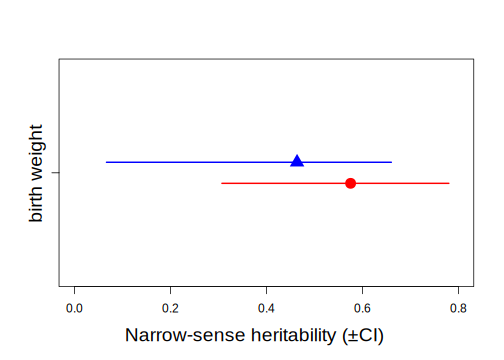
\includegraphics{wam_tuto_files/figure-latex/unnamed-chunk-72-1.pdf}
\caption{\label{fig:unnamed-chunk-72}Female and male heritability of birth weight}
\end{figure}

\hypertarget{modification-of-model-parameter-1}{%
\subsection{Modification of model parameter}\label{modification-of-model-parameter-1}}

Unfortunately (to our knowledge), it is not possible to alter the variance matrices and refit them within the model.

\hypertarget{covariance-between-two-random-effects-2}{%
\subsection{Covariance between two random effects}\label{covariance-between-two-random-effects-2}}

Some research questions require to estimate the covariance between two random effects within a univariate model.
Unfortunately (to our knowledge), it is not possible to create a covariance between distinct random effects (\url{https://github.com/paul-buerkner/brms/issues/502}).
However,a multi-membership model can be fit using the linking.function \texttt{mm}, thus forcing the variance of two variables to be equal and the covariance to 1.

\hypertarget{stan}{%
\section{stan}\label{stan}}

to do

\hypertarget{multivariate-animal-model}{%
\chapter{Multivariate animal model}\label{multivariate-animal-model}}

This tutorial will demonstrate how to run a multivariate animal model looking at birth weight and tarsus length of the phenomenal gryphons.

\hypertarget{scenario-and-data-1}{%
\section{Scenario and data}\label{scenario-and-data-1}}

\hypertarget{scenario-1}{%
\subsection{Scenario}\label{scenario-1}}

Since natural selection rarely acts on single traits, to understand how birth weight might evolve in our population of gryphons, we may also want to think about possible covariance with other traits. If tarsus length at fledging is also under positive selection, what implications does it have for birth weight and vice versa? If the two traits are positively genetically correlated then this will facilitate evolution of larger size (since response of one trait will induce a positively correlated response in the other). If there is negative genetic covariance then this could act as an evolutionary constraint.

Using multivariate models allows the estimation of parameters relating to each trait alone (\emph{i.e.} \(V_A\), \(h^2\), etc), but also yields estimates of covariance components between traits. These include the (additive) genetic covariance \(COV_A\) which is often rescaled to give the additive genetic correlation \(r_A\). However, covariance can also arise through other random effects (\emph{e.g.} maternal covariance) and these sources can also be explicitly modeled in a bivariate analysis.

\hypertarget{gryphon-files}{%
\subsection{gryphon files}\label{gryphon-files}}

gryphonpedigree and phenotypic data files are the same as those used in tutorial 1 (\emph{i.e}, \texttt{gryphonped.csv} and \texttt{gryphon.csv} respectively).

Reading the data

\begin{Shaded}
\begin{Highlighting}[]
\NormalTok{gryphon \textless{}{-}}\StringTok{ }\KeywordTok{read.csv}\NormalTok{(}\StringTok{"data/gryphon.csv"}\NormalTok{)}
\NormalTok{gryphon}\OperatorTok{$}\NormalTok{animal \textless{}{-}}\StringTok{ }\KeywordTok{as.factor}\NormalTok{(gryphon}\OperatorTok{$}\NormalTok{animal)}
\NormalTok{gryphon}\OperatorTok{$}\NormalTok{mother \textless{}{-}}\StringTok{ }\KeywordTok{as.factor}\NormalTok{(gryphon}\OperatorTok{$}\NormalTok{mother)}
\NormalTok{gryphon}\OperatorTok{$}\NormalTok{byear \textless{}{-}}\StringTok{ }\KeywordTok{as.factor}\NormalTok{(gryphon}\OperatorTok{$}\NormalTok{byear)}
\NormalTok{gryphon}\OperatorTok{$}\NormalTok{sex \textless{}{-}}\StringTok{ }\KeywordTok{as.factor}\NormalTok{(gryphon}\OperatorTok{$}\NormalTok{sex)}
\NormalTok{gryphon}\OperatorTok{$}\NormalTok{bwt \textless{}{-}}\StringTok{ }\KeywordTok{as.numeric}\NormalTok{(gryphon}\OperatorTok{$}\NormalTok{bwt)}
\NormalTok{gryphon}\OperatorTok{$}\NormalTok{tarsus \textless{}{-}}\StringTok{ }\KeywordTok{as.numeric}\NormalTok{(gryphon}\OperatorTok{$}\NormalTok{tarsus)}
\end{Highlighting}
\end{Shaded}

Reading the pedigree

\begin{Shaded}
\begin{Highlighting}[]
\NormalTok{gryphonped \textless{}{-}}\StringTok{ }\KeywordTok{read.csv}\NormalTok{(}\StringTok{"data/gryphonped.csv"}\NormalTok{)}
\NormalTok{gryphonped}\OperatorTok{$}\NormalTok{id \textless{}{-}}\StringTok{ }\KeywordTok{as.factor}\NormalTok{(gryphonped}\OperatorTok{$}\NormalTok{id)}
\NormalTok{gryphonped}\OperatorTok{$}\NormalTok{father \textless{}{-}}\StringTok{ }\KeywordTok{as.factor}\NormalTok{(gryphonped}\OperatorTok{$}\NormalTok{father)}
\NormalTok{gryphonped}\OperatorTok{$}\NormalTok{mother \textless{}{-}}\StringTok{ }\KeywordTok{as.factor}\NormalTok{(gryphonped}\OperatorTok{$}\NormalTok{mother)}
\end{Highlighting}
\end{Shaded}

\hypertarget{asreml-biv}{%
\section{Asreml-R}\label{asreml-biv}}

\hypertarget{running-the-model-3}{%
\subsection{Running the model}\label{running-the-model-3}}

First we need to load the \texttt{asreml} library:

\begin{Shaded}
\begin{Highlighting}[]
\KeywordTok{library}\NormalTok{(asreml)}
\end{Highlighting}
\end{Shaded}

For running multivariate analyses in ASReml-R, the code is slightly more complex than for the univariate case. This is because ASReml-R allows us to make different assumptions about the way in which traits might be related. We need to explicitly specify a covariance structure with difference covariance functions \texttt{us()}, \texttt{idh()} or \texttt{corgh()} which for example would estimate an unconstrained (co)variance matrix, an identity matrix and a variance and correlation matrix repestively. We can also specify some starting values for the variance matrices. These can be very approximate \emph{guestimates} or not at all, but having reasonable starting values can help convergence. It is also possible to let the model running without specifying starting values. Finally, we have increased the default maximum number of iterations (\texttt{maxiter}) which can help to achieve convergence for more complicated models. Another way to increase the number of iteration will be to use the \texttt{update} function. Notes that if the \texttt{LogLik} is not stabilized after several iterations, it is good indication of the model require more iteration.

\begin{Shaded}
\begin{Highlighting}[]
\NormalTok{ainv \textless{}{-}}\StringTok{ }\KeywordTok{ainverse}\NormalTok{(gryphonped)}
\NormalTok{modela \textless{}{-}}\StringTok{ }\KeywordTok{asreml}\NormalTok{(}
  \DataTypeTok{fixed =} \KeywordTok{cbind}\NormalTok{(bwt, tarsus) }\OperatorTok{\textasciitilde{}}\StringTok{ }\NormalTok{trait,}
  \DataTypeTok{random =} \OperatorTok{\textasciitilde{}}\StringTok{ }\KeywordTok{us}\NormalTok{(trait, }\DataTypeTok{init =} \KeywordTok{c}\NormalTok{(}\DecValTok{1}\NormalTok{, }\FloatTok{0.1}\NormalTok{, }\DecValTok{1}\NormalTok{))}\OperatorTok{:}\KeywordTok{vm}\NormalTok{(animal, ainv),}
  \DataTypeTok{residual =} \OperatorTok{\textasciitilde{}}\StringTok{ }\KeywordTok{id}\NormalTok{(units)}\OperatorTok{:}\KeywordTok{us}\NormalTok{(trait, }\DataTypeTok{init =} \KeywordTok{c}\NormalTok{(}\DecValTok{1}\NormalTok{, }\FloatTok{0.1}\NormalTok{, }\DecValTok{1}\NormalTok{)),}
  \DataTypeTok{data =}\NormalTok{ gryphon,}
  \DataTypeTok{na.action =} \KeywordTok{na.method}\NormalTok{(}\DataTypeTok{x =} \StringTok{"include"}\NormalTok{, }\DataTypeTok{y =} \StringTok{"include"}\NormalTok{),}
  \DataTypeTok{maxit =} \DecValTok{20}
\NormalTok{)}
\end{Highlighting}
\end{Shaded}

\begin{verbatim}
## Model fitted using the sigma parameterization.
## ASReml 4.1.0 Sat Apr 30 11:10:25 2022
##           LogLik        Sigma2     DF     wall    cpu
##  1     -7108.741           1.0   1535 11:10:25    0.0
##  2     -5837.803           1.0   1535 11:10:25    0.0
##  3     -4437.495           1.0   1535 11:10:25    0.0
##  4     -3459.378           1.0   1535 11:10:25    0.0
##  5     -2914.034           1.0   1535 11:10:25    0.0
##  6     -2729.131           1.0   1535 11:10:25    0.0
##  7     -2684.659           1.0   1535 11:10:25    0.0
##  8     -2679.838           1.0   1535 11:10:25    0.0
##  9     -2679.742           1.0   1535 11:10:25    0.0
## 10     -2679.741           1.0   1535 11:10:25    0.0
\end{verbatim}

\begin{Shaded}
\begin{Highlighting}[]
\NormalTok{modela \textless{}{-}}\StringTok{ }\KeywordTok{update}\NormalTok{(modela)}
\end{Highlighting}
\end{Shaded}

\begin{verbatim}
## Model fitted using the sigma parameterization.
## ASReml 4.1.0 Sat Apr 30 11:10:25 2022
##           LogLik        Sigma2     DF     wall    cpu
##  1     -2679.741           1.0   1535 11:10:25    0.0
##  2     -2679.741           1.0   1535 11:10:25    0.0
\end{verbatim}

\texttt{modela} has fitted a bivariate model of \texttt{bwt} and \texttt{tarsus}, with the mean for each of the traits as a fixed effect (\texttt{trait}). The additive genetic variance-covariance matrix (\(\textbf{G}\)) is unstructured (\texttt{us}; \emph{i.e.} all elements are free to vary) and the starting values for \(V_A\) for \texttt{bwt}, \(COV_A\) between \texttt{bwt} and \texttt{tarsus}, and \(V_A\) for \texttt{tarsus} are set to 1, 0.1 and 1, respectively. Similarly, the residual matrix is unstructured and uses the same starting values.

Note that the argument \texttt{na.action\ =\ na.method(x\ =\ "include",\ y\ =\ "include")} can be added to the model. In a bivariate model, it will help calculate the covariance between two traits with different missing information \texttt{NA} and so help imbalance phenotypage and save sample size. However, it is important to scale ( mean =0, var =1) the two traits to correctly adjust the model(see Asreml-R manual for more information).

Let's have a look at the variance components, and notice that there are now seven (co)variance components reported in the table:

\begin{Shaded}
\begin{Highlighting}[]
\KeywordTok{summary}\NormalTok{(modela)}\OperatorTok{$}\NormalTok{varcomp}
\end{Highlighting}
\end{Shaded}

\begin{verbatim}
##                                            component std.error  z.ratio bound
## trait:vm(animal, ainv)!trait_bwt:bwt        3.368397 0.6348307 5.305977     P
## trait:vm(animal, ainv)!trait_tarsus:bwt     2.459809 1.0732644 2.291895     P
## trait:vm(animal, ainv)!trait_tarsus:tarsus 12.345792 3.0744285 4.015638     P
## units:trait!R                               1.000000        NA       NA     F
## units:trait!trait_bwt:bwt                   3.849916 0.5200101 7.403541     P
## units:trait!trait_tarsus:bwt                3.313282 0.9129234 3.629310     P
## units:trait!trait_tarsus:tarsus            17.646432 2.6670380 6.616491     P
##                                            %ch
## trait:vm(animal, ainv)!trait_bwt:bwt         0
## trait:vm(animal, ainv)!trait_tarsus:bwt      0
## trait:vm(animal, ainv)!trait_tarsus:tarsus   0
## units:trait!R                                0
## units:trait!trait_bwt:bwt                    0
## units:trait!trait_tarsus:bwt                 0
## units:trait!trait_tarsus:tarsus              0
\end{verbatim}

The first three terms are related to the genetic matrix and, in order are \(V_{A,bwt}\), \(COV_A\), \(V_{A, tarsus}\). Below is again a line where the \texttt{units:traitr!R} component equals to 1, which again can be ignored. The final three terms relate to the residual matrix and correspond to \(V_{R,bwt}\), \(COV_R\), \(V_{R,tarsus}\). Based on our quick and dirty check (is \texttt{z.ratio} \textgreater{} 1.96?) all components look to be statistically significant.

We can calculate the genetic correlation as \(COV_A / \sqrt{V_{A,bwt} \cdot V_{A,tarsus}}\). Thus this model gives an estimate of \(r_A\) = 0.38. It is also possible to estimate the residual correlation \(r_{res}\) = 0.4.

Both correlations are distinct in nature. The genetic correlation reflects how much the traits are linked by genetic via polygenic effect or linkage desequilibrium, whereas the residual correlation reflects the environmental correlation or errors measurement correlation.

Although we can calculate this by hand, we can also use \texttt{vpredict()}, which also provides an (approximate) standard error:

\begin{Shaded}
\begin{Highlighting}[]
\KeywordTok{vpredict}\NormalTok{(modela, r\_A }\OperatorTok{\textasciitilde{}}\StringTok{ }\NormalTok{V2 }\OperatorTok{/}\StringTok{ }\KeywordTok{sqrt}\NormalTok{(V1 }\OperatorTok{*}\StringTok{ }\NormalTok{V3))}
\end{Highlighting}
\end{Shaded}

\begin{verbatim}
##      Estimate        SE
## r_A 0.3814436 0.1299759
\end{verbatim}

\begin{Shaded}
\begin{Highlighting}[]
\KeywordTok{vpredict}\NormalTok{(modela, r\_res }\OperatorTok{\textasciitilde{}}\StringTok{ }\NormalTok{V6 }\OperatorTok{/}\StringTok{ }\KeywordTok{sqrt}\NormalTok{(V5 }\OperatorTok{*}\StringTok{ }\NormalTok{V7))}
\end{Highlighting}
\end{Shaded}

\begin{verbatim}
##        Estimate         SE
## r_res 0.4019799 0.08607104
\end{verbatim}

Of course we can also calculate the heritability of \texttt{bwt} and \texttt{tarsus} from this model:

\begin{Shaded}
\begin{Highlighting}[]
\KeywordTok{vpredict}\NormalTok{(modela, h2.bwt }\OperatorTok{\textasciitilde{}}\StringTok{ }\NormalTok{V1 }\OperatorTok{/}\StringTok{ }\NormalTok{(V1 }\OperatorTok{+}\StringTok{ }\NormalTok{V5))}
\end{Highlighting}
\end{Shaded}

\begin{verbatim}
##        Estimate         SE
## h2.bwt 0.466646 0.07671533
\end{verbatim}

\begin{Shaded}
\begin{Highlighting}[]
\KeywordTok{vpredict}\NormalTok{(modela, h2.tarsus }\OperatorTok{\textasciitilde{}}\StringTok{ }\NormalTok{V3 }\OperatorTok{/}\StringTok{ }\NormalTok{(V3 }\OperatorTok{+}\StringTok{ }\NormalTok{V7))}
\end{Highlighting}
\end{Shaded}

\begin{verbatim}
##            Estimate         SE
## h2.tarsus 0.4116331 0.09305863
\end{verbatim}

\hypertarget{adding-fixed-and-random-effects}{%
\subsection{Adding fixed and random effects}\label{adding-fixed-and-random-effects}}

Fixed and random effects can be added just as for the univariate case. Given that our full model of bwt from tutorial 1 had sex as a fixed effect as well as birth year and mother as random effects, we could specify a bivariate formulation with the same complexity:

\begin{Shaded}
\begin{Highlighting}[]
\NormalTok{modelb \textless{}{-}}\StringTok{ }\KeywordTok{asreml}\NormalTok{(}
  \DataTypeTok{fixed =} \KeywordTok{cbind}\NormalTok{(bwt, tarsus) }\OperatorTok{\textasciitilde{}}\StringTok{ }\NormalTok{trait }\OperatorTok{+}\StringTok{ }\KeywordTok{at}\NormalTok{(trait)}\OperatorTok{:}\NormalTok{sex,}
  \DataTypeTok{random =} \OperatorTok{\textasciitilde{}}\StringTok{ }\KeywordTok{us}\NormalTok{(trait, }\DataTypeTok{init =} \KeywordTok{c}\NormalTok{(}\DecValTok{1}\NormalTok{, }\FloatTok{0.1}\NormalTok{, }\DecValTok{1}\NormalTok{))}\OperatorTok{:}\KeywordTok{vm}\NormalTok{(animal, ainv) }\OperatorTok{+}
\StringTok{    }\KeywordTok{us}\NormalTok{(trait, }\DataTypeTok{init =} \KeywordTok{c}\NormalTok{(}\DecValTok{1}\NormalTok{, }\FloatTok{0.1}\NormalTok{, }\DecValTok{1}\NormalTok{))}\OperatorTok{:}\NormalTok{byear }\OperatorTok{+}
\StringTok{    }\KeywordTok{us}\NormalTok{(trait, }\DataTypeTok{init =} \KeywordTok{c}\NormalTok{(}\DecValTok{1}\NormalTok{, }\FloatTok{0.1}\NormalTok{, }\DecValTok{1}\NormalTok{))}\OperatorTok{:}\NormalTok{mother,}
  \DataTypeTok{residual =} \OperatorTok{\textasciitilde{}}\StringTok{ }\KeywordTok{id}\NormalTok{(units)}\OperatorTok{:}\KeywordTok{us}\NormalTok{(trait, }\DataTypeTok{init =} \KeywordTok{c}\NormalTok{(}\DecValTok{1}\NormalTok{, }\FloatTok{0.1}\NormalTok{, }\DecValTok{1}\NormalTok{)),}
  \DataTypeTok{data =}\NormalTok{ gryphon,}
  \DataTypeTok{na.action =} \KeywordTok{na.method}\NormalTok{(}\DataTypeTok{x =} \StringTok{"include"}\NormalTok{, }\DataTypeTok{y =} \StringTok{"include"}\NormalTok{),}
  \DataTypeTok{maxit =} \DecValTok{20}
\NormalTok{)}
\end{Highlighting}
\end{Shaded}

\begin{verbatim}
## Model fitted using the sigma parameterization.
## ASReml 4.1.0 Sat Apr 30 11:10:25 2022
##           LogLik        Sigma2     DF     wall    cpu
##  1     -4672.301           1.0   1533 11:10:25    0.0
##  2     -4005.615           1.0   1533 11:10:25    0.0
##  3     -3271.483           1.0   1533 11:10:25    0.0 (1 restrained)
##  4     -2761.414           1.0   1533 11:10:25    0.0 (1 restrained)
##  5     -2481.357           1.0   1533 11:10:25    0.0
##  6     -2395.858           1.0   1533 11:10:25    0.0
##  7     -2381.050           1.0   1533 11:10:25    0.0
##  8     -2380.251           1.0   1533 11:10:25    0.0
##  9     -2380.246           1.0   1533 11:10:25    0.0
\end{verbatim}

\begin{Shaded}
\begin{Highlighting}[]
\NormalTok{modelb \textless{}{-}}\StringTok{ }\KeywordTok{update}\NormalTok{(modelb)}
\end{Highlighting}
\end{Shaded}

\begin{verbatim}
## Model fitted using the sigma parameterization.
## ASReml 4.1.0 Sat Apr 30 11:10:25 2022
##           LogLik        Sigma2     DF     wall    cpu
##  1     -2380.246           1.0   1533 11:10:25    0.0
##  2     -2380.246           1.0   1533 11:10:25    0.0
\end{verbatim}

Note that we have specified a covariance structure for each random effect and an estimate of the effect of sex on both birth weight and tarsus length.

There will now be thirteen (co)variance components reported after running the code:

\begin{Shaded}
\begin{Highlighting}[]
\KeywordTok{summary}\NormalTok{(modelb)}\OperatorTok{$}\NormalTok{varcomp}
\end{Highlighting}
\end{Shaded}

\begin{verbatim}
##                                             component std.error    z.ratio
## trait:byear!trait_bwt:bwt                   0.9746385 0.2825727  3.4491602
## trait:byear!trait_tarsus:bwt                0.1624076 0.4185079  0.3880635
## trait:byear!trait_tarsus:tarsus             3.7383721 1.2065992  3.0982716
## trait:mother!trait_bwt:bwt                  1.1445184 0.2302182  4.9714512
## trait:mother!trait_tarsus:bwt              -1.5567306 0.4051848 -3.8420260
## trait:mother!trait_tarsus:tarsus            4.8206132 1.3201300  3.6516202
## trait:vm(animal, ainv)!trait_bwt:bwt        1.9893546 0.4410246  4.5107569
## trait:vm(animal, ainv)!trait_tarsus:bwt     3.3170404 0.9032323  3.6724110
## trait:vm(animal, ainv)!trait_tarsus:tarsus 10.2294887 2.8077066  3.6433610
## units:trait!R                               1.0000000        NA         NA
## units:trait!trait_bwt:bwt                   1.8443110 0.3443178  5.3564203
## units:trait!trait_tarsus:bwt                4.0142841 0.7412540  5.4155308
## units:trait!trait_tarsus:tarsus            12.4845955 2.2893363  5.4533690
##                                            bound %ch
## trait:byear!trait_bwt:bwt                      P   0
## trait:byear!trait_tarsus:bwt                   P   0
## trait:byear!trait_tarsus:tarsus                P   0
## trait:mother!trait_bwt:bwt                     P   0
## trait:mother!trait_tarsus:bwt                  P   0
## trait:mother!trait_tarsus:tarsus               P   0
## trait:vm(animal, ainv)!trait_bwt:bwt           P   0
## trait:vm(animal, ainv)!trait_tarsus:bwt        P   0
## trait:vm(animal, ainv)!trait_tarsus:tarsus     P   0
## units:trait!R                                  F   0
## units:trait!trait_bwt:bwt                      P   0
## units:trait!trait_tarsus:bwt                   P   0
## units:trait!trait_tarsus:tarsus                P   0
\end{verbatim}

we can estimate the different correlations using \texttt{vpredict}:

\begin{Shaded}
\begin{Highlighting}[]
\KeywordTok{vpredict}\NormalTok{(modelb, r\_byear }\OperatorTok{\textasciitilde{}}\StringTok{ }\NormalTok{V2 }\OperatorTok{/}\StringTok{ }\KeywordTok{sqrt}\NormalTok{(V1 }\OperatorTok{*}\StringTok{ }\NormalTok{V3))}
\end{Highlighting}
\end{Shaded}

\begin{verbatim}
##           Estimate        SE
## r_byear 0.08508312 0.2134209
\end{verbatim}

\begin{Shaded}
\begin{Highlighting}[]
\KeywordTok{vpredict}\NormalTok{(modelb, r\_M }\OperatorTok{\textasciitilde{}}\StringTok{ }\NormalTok{V5 }\OperatorTok{/}\StringTok{ }\KeywordTok{sqrt}\NormalTok{(V4 }\OperatorTok{*}\StringTok{ }\NormalTok{V6))}
\end{Highlighting}
\end{Shaded}

\begin{verbatim}
##       Estimate        SE
## r_M -0.6627518 0.2487963
\end{verbatim}

\begin{Shaded}
\begin{Highlighting}[]
\KeywordTok{vpredict}\NormalTok{(modelb, r\_A }\OperatorTok{\textasciitilde{}}\StringTok{ }\NormalTok{V8 }\OperatorTok{/}\StringTok{ }\KeywordTok{sqrt}\NormalTok{(V7 }\OperatorTok{*}\StringTok{ }\NormalTok{V9))}
\end{Highlighting}
\end{Shaded}

\begin{verbatim}
##      Estimate        SE
## r_A 0.7353053 0.1094747
\end{verbatim}

\begin{Shaded}
\begin{Highlighting}[]
\KeywordTok{vpredict}\NormalTok{(modelb, r\_res }\OperatorTok{\textasciitilde{}}\StringTok{ }\NormalTok{V12 }\OperatorTok{/}\StringTok{ }\KeywordTok{sqrt}\NormalTok{(V11 }\OperatorTok{*}\StringTok{ }\NormalTok{V13))}
\end{Highlighting}
\end{Shaded}

\begin{verbatim}
##        Estimate         SE
## r_res 0.8365729 0.07366762
\end{verbatim}

Now we can look at the fixed effects parameters and assess their significance with a conditional Wald F-test:

\begin{Shaded}
\begin{Highlighting}[]
\KeywordTok{summary}\NormalTok{(modelb, }\DataTypeTok{coef =} \OtherTok{TRUE}\NormalTok{)}\OperatorTok{$}\NormalTok{coef.fi}
\KeywordTok{wald.asreml}\NormalTok{(modelb, }\DataTypeTok{denDF =} \StringTok{"default"}\NormalTok{, }\DataTypeTok{ssType =} \StringTok{"conditional"}\NormalTok{)}\OperatorTok{$}\NormalTok{Wald}
\end{Highlighting}
\end{Shaded}

\begin{verbatim}
##                           solution std error    z.ratio
## at(trait, tarsus):sex_1  0.0000000        NA         NA
## at(trait, tarsus):sex_2 -0.0684413 0.3823448 -0.1790041
## at(trait, bwt):sex_1     0.0000000        NA         NA
## at(trait, bwt):sex_2     1.9502053 0.1480467 13.1729086
## trait_bwt                6.3844483 0.2328210 27.4221324
## trait_tarsus            20.5936436 0.5098944 40.3880569
\end{verbatim}

\begin{verbatim}
## Model fitted using the sigma parameterization.
## ASReml 4.1.0 Sat Apr 30 11:10:25 2022
##           LogLik        Sigma2     DF     wall    cpu
##  1     -2380.246           1.0   1533 11:10:26    0.0
##  2     -2380.246           1.0   1533 11:10:26    0.0
## Calculating denominator DF
\end{verbatim}

\begin{verbatim}
## 
##                       Df denDF   F.inc   F.con Margin      Pr
## trait                  2  52.6 1396.00 1396.00        0.00000
## at(trait, bwt):sex     1 812.8  298.40  173.50      B 0.00000
## at(trait, tarsus):sex  1 747.9    0.03    0.03      B 0.85798
\end{verbatim}

Note that it is possible to specify a fixed effect to a specific trait by adding the number of order within \texttt{cbind} inside the argument \texttt{at(trait,x)}. For example, here we apply the fixed effect \texttt{sex} only to the response variable \texttt{tarsus}.

\begin{Shaded}
\begin{Highlighting}[]
\NormalTok{modelb\_}\DecValTok{2}\NormalTok{ \textless{}{-}}\StringTok{ }\KeywordTok{asreml}\NormalTok{(}
  \DataTypeTok{fixed =} \KeywordTok{cbind}\NormalTok{(bwt, tarsus) }\OperatorTok{\textasciitilde{}}\StringTok{ }\NormalTok{trait }\OperatorTok{+}\StringTok{ }\KeywordTok{at}\NormalTok{(trait, }\DecValTok{2}\NormalTok{)}\OperatorTok{:}\NormalTok{sex,}
  \DataTypeTok{random =} \OperatorTok{\textasciitilde{}}\StringTok{ }\KeywordTok{us}\NormalTok{(trait, }\DataTypeTok{init =} \KeywordTok{c}\NormalTok{(}\DecValTok{1}\NormalTok{, }\FloatTok{0.1}\NormalTok{, }\DecValTok{1}\NormalTok{))}\OperatorTok{:}\KeywordTok{vm}\NormalTok{(animal, ainv) }\OperatorTok{+}
\StringTok{    }\KeywordTok{us}\NormalTok{(trait, }\DataTypeTok{init =} \KeywordTok{c}\NormalTok{(}\DecValTok{1}\NormalTok{, }\FloatTok{0.1}\NormalTok{, }\DecValTok{1}\NormalTok{))}\OperatorTok{:}\NormalTok{byear }\OperatorTok{+}
\StringTok{    }\KeywordTok{us}\NormalTok{(trait, }\DataTypeTok{init =} \KeywordTok{c}\NormalTok{(}\DecValTok{1}\NormalTok{, }\FloatTok{0.1}\NormalTok{, }\DecValTok{1}\NormalTok{))}\OperatorTok{:}\NormalTok{mother,}
  \DataTypeTok{residual =} \OperatorTok{\textasciitilde{}}\StringTok{ }\KeywordTok{id}\NormalTok{(units)}\OperatorTok{:}\KeywordTok{us}\NormalTok{(trait, }\DataTypeTok{init =} \KeywordTok{c}\NormalTok{(}\DecValTok{1}\NormalTok{, }\FloatTok{0.1}\NormalTok{, }\DecValTok{1}\NormalTok{)),}
  \DataTypeTok{data =}\NormalTok{ gryphon,}
  \DataTypeTok{na.action =} \KeywordTok{na.method}\NormalTok{(}\DataTypeTok{x =} \StringTok{"include"}\NormalTok{, }\DataTypeTok{y =} \StringTok{"include"}\NormalTok{),}
  \DataTypeTok{maxit =} \DecValTok{20}
\NormalTok{)}
\end{Highlighting}
\end{Shaded}

\begin{verbatim}
## Model fitted using the sigma parameterization.
## ASReml 4.1.0 Sat Apr 30 11:10:26 2022
##           LogLik        Sigma2     DF     wall    cpu
##  1     -4810.563           1.0   1534 11:10:26    0.0
##  2     -4129.799           1.0   1534 11:10:26    0.0
##  3     -3382.529           1.0   1534 11:10:26    0.0 (1 restrained)
##  4     -2864.076           1.0   1534 11:10:26    0.0
##  5     -2574.891           1.0   1534 11:10:26    0.0
##  6     -2478.879           1.0   1534 11:10:26    0.0
##  7     -2458.305           1.0   1534 11:10:26    0.0
##  8     -2456.425           1.0   1534 11:10:26    0.0
##  9     -2456.377           1.0   1534 11:10:26    0.0
## 10     -2456.376           1.0   1534 11:10:26    0.0
\end{verbatim}

\begin{Shaded}
\begin{Highlighting}[]
\KeywordTok{summary}\NormalTok{(modelb\_}\DecValTok{2}\NormalTok{, }\DataTypeTok{coef =} \OtherTok{TRUE}\NormalTok{)}\OperatorTok{$}\NormalTok{coef.fi}
\KeywordTok{wald.asreml}\NormalTok{(modelb\_}\DecValTok{2}\NormalTok{, }\DataTypeTok{denDF =} \StringTok{"default"}\NormalTok{, }\DataTypeTok{ssType =} \StringTok{"conditional"}\NormalTok{)}\OperatorTok{$}\NormalTok{Wald}
\end{Highlighting}
\end{Shaded}

\begin{verbatim}
##                          solution std error   z.ratio
## at(trait, tarsus):sex_1  0.000000        NA        NA
## at(trait, tarsus):sex_2 -3.267042 0.2953279 -11.06242
## trait_bwt                7.636226 0.2389515  31.95722
## trait_tarsus            22.703658 0.4827348  47.03133
\end{verbatim}

\begin{verbatim}
## Model fitted using the sigma parameterization.
## ASReml 4.1.0 Sat Apr 30 11:10:26 2022
##           LogLik        Sigma2     DF     wall    cpu
##  1     -2456.376           1.0   1534 11:10:26    0.0
##  2     -2456.376           1.0   1534 11:10:26    0.0
## Calculating denominator DF
\end{verbatim}

\begin{verbatim}
## 
##                       Df denDF  F.inc  F.con Margin          Pr
## trait                  2  50.7 1233.0 1233.0        0.00000e+00
## at(trait, tarsus):sex  1 522.9  122.4  122.4      B 1.02886e-25
\end{verbatim}

\hypertarget{significance-testing}{%
\subsection{Significance testing}\label{significance-testing}}

Under the model above \(r_M\) is estimated as -0.66 and the \texttt{z.ratio} associated with the corresponding covariance (\(COV_M\)) is \textgreater2 (in absolute terms). We might therefore infer that there is evidence for a strong negative correlation between the traits with respect to the mother and that while maternal identity explains variance in both traits those mothers that tend to produce heavier offspring actually tend to produce offspring with shorter tarsus lengths.

To formally test if \(COV_M\) is significantly different from zero, we can compare the log-likelihood for this model:

\begin{Shaded}
\begin{Highlighting}[]
\NormalTok{modelb}\OperatorTok{$}\NormalTok{loglik}
\end{Highlighting}
\end{Shaded}

\begin{verbatim}
## [1] -2380.246
\end{verbatim}

to a model in which we specify that \(COV_M\)=0. Since this constraint reduces the number of parameters to be estimated by one, we can use a likelihood ratio test (LRT) with one degree of freedom. To run the constrained model, we modify the G structure defined for the \texttt{mother} random effect to diagonal (\texttt{diag}), which means we only estimate the variances (the diagonal of the matrix) but not the covariance (the covariance are fixed to 0):

\begin{Shaded}
\begin{Highlighting}[]
\NormalTok{modelc \textless{}{-}}\StringTok{ }\KeywordTok{asreml}\NormalTok{(}
  \DataTypeTok{fixed =} \KeywordTok{cbind}\NormalTok{(bwt, tarsus) }\OperatorTok{\textasciitilde{}}\StringTok{ }\NormalTok{trait }\OperatorTok{+}\StringTok{ }\KeywordTok{at}\NormalTok{(trait)}\OperatorTok{:}\NormalTok{sex,}
  \DataTypeTok{random =} \OperatorTok{\textasciitilde{}}\StringTok{ }\KeywordTok{us}\NormalTok{(trait, }\DataTypeTok{init =} \KeywordTok{c}\NormalTok{(}\DecValTok{1}\NormalTok{, }\FloatTok{0.1}\NormalTok{, }\DecValTok{1}\NormalTok{))}\OperatorTok{:}\KeywordTok{vm}\NormalTok{(animal, ainv) }\OperatorTok{+}
\StringTok{    }\KeywordTok{us}\NormalTok{(trait, }\DataTypeTok{init =} \KeywordTok{c}\NormalTok{(}\DecValTok{1}\NormalTok{, }\FloatTok{0.1}\NormalTok{, }\DecValTok{1}\NormalTok{))}\OperatorTok{:}\NormalTok{byear }\OperatorTok{+}
\StringTok{    }\KeywordTok{diag}\NormalTok{(trait, }\DataTypeTok{init =} \KeywordTok{c}\NormalTok{(}\DecValTok{1}\NormalTok{, }\DecValTok{1}\NormalTok{))}\OperatorTok{:}\NormalTok{mother,}
  \DataTypeTok{residual =} \OperatorTok{\textasciitilde{}}\StringTok{ }\KeywordTok{id}\NormalTok{(units)}\OperatorTok{:}\KeywordTok{us}\NormalTok{(trait, }\DataTypeTok{init =} \KeywordTok{c}\NormalTok{(}\DecValTok{1}\NormalTok{, }\FloatTok{0.1}\NormalTok{, }\DecValTok{1}\NormalTok{)),}
  \DataTypeTok{data =}\NormalTok{ gryphon,}
  \DataTypeTok{na.action =} \KeywordTok{na.method}\NormalTok{(}\DataTypeTok{x =} \StringTok{"include"}\NormalTok{, }\DataTypeTok{y =} \StringTok{"include"}\NormalTok{),}
  \DataTypeTok{maxit =} \DecValTok{20}
\NormalTok{)}
\end{Highlighting}
\end{Shaded}

\begin{verbatim}
## Model fitted using the sigma parameterization.
## ASReml 4.1.0 Sat Apr 30 11:10:27 2022
##           LogLik        Sigma2     DF     wall    cpu
##  1     -4677.820           1.0   1533 11:10:27    0.0
##  2     -4010.442           1.0   1533 11:10:27    0.0
##  3     -3275.409           1.0   1533 11:10:27    0.0
##  4     -2763.519           1.0   1533 11:10:27    0.0
##  5     -2483.732           1.0   1533 11:10:27    0.0
##  6     -2400.242           1.0   1533 11:10:27    0.0
##  7     -2386.663           1.0   1533 11:10:27    0.0
##  8     -2386.049           1.0   1533 11:10:27    0.0
##  9     -2386.045           1.0   1533 11:10:27    0.0
\end{verbatim}

You can run \texttt{summary(modelc)\$varcomp} to confirm this worked. We can now obtain the log-likelihood of this model and compare this to that of \texttt{modelb} using a likelihood ratio test:

\begin{Shaded}
\begin{Highlighting}[]
\NormalTok{modelc}\OperatorTok{$}\NormalTok{loglik}
\end{Highlighting}
\end{Shaded}

\begin{verbatim}
## [1] -2386.045
\end{verbatim}

We can see that the model log-likelihood is now -2386.05.
And comparing the models using a likelihood ratio test:

\begin{Shaded}
\begin{Highlighting}[]
\DecValTok{2} \OperatorTok{*}\StringTok{ }\NormalTok{(modelb}\OperatorTok{$}\NormalTok{loglik }\OperatorTok{{-}}\StringTok{ }\NormalTok{modelc}\OperatorTok{$}\NormalTok{loglik)}
\end{Highlighting}
\end{Shaded}

\begin{verbatim}
## [1] 11.59835
\end{verbatim}

So our chi-square test statistic is \(\chi^2_1\)= 11.6.
The p-value that goes with this is obtained by:

\begin{Shaded}
\begin{Highlighting}[]
\DecValTok{1} \OperatorTok{{-}}\StringTok{ }\KeywordTok{pchisq}\NormalTok{(}\DecValTok{2} \OperatorTok{*}\StringTok{ }\NormalTok{(modelb}\OperatorTok{$}\NormalTok{loglik }\OperatorTok{{-}}\StringTok{ }\NormalTok{modelc}\OperatorTok{$}\NormalTok{loglik), }\DecValTok{1}\NormalTok{)}
\end{Highlighting}
\end{Shaded}

\begin{verbatim}
## [1] 0.0006601037
\end{verbatim}

We would therefore conclude that the maternal covariance is significantly different from zero.

We could apply the same procedure to show that the residual (environmental) covariance and the genetic covariance estimates are significantly greater than zero (\emph{i.e.}, heavier individuals tend to have longer tarsus lengths). In contrast, we should find that the byear covariance between the two traits is non-significant.

\begin{Shaded}
\begin{Highlighting}[]
\NormalTok{modeld \textless{}{-}}\StringTok{ }\KeywordTok{asreml}\NormalTok{(}
  \DataTypeTok{fixed =} \KeywordTok{cbind}\NormalTok{(bwt, tarsus) }\OperatorTok{\textasciitilde{}}\StringTok{ }\NormalTok{trait }\OperatorTok{+}\StringTok{ }\KeywordTok{at}\NormalTok{(trait)}\OperatorTok{:}\NormalTok{sex,}
  \DataTypeTok{random =} \OperatorTok{\textasciitilde{}}\StringTok{ }\KeywordTok{us}\NormalTok{(trait, }\DataTypeTok{init =} \KeywordTok{c}\NormalTok{(}\DecValTok{1}\NormalTok{, }\FloatTok{0.1}\NormalTok{, }\DecValTok{1}\NormalTok{))}\OperatorTok{:}\KeywordTok{vm}\NormalTok{(animal, ainv) }\OperatorTok{+}
\StringTok{    }\KeywordTok{diag}\NormalTok{(trait, }\DataTypeTok{init =} \KeywordTok{c}\NormalTok{(}\DecValTok{1}\NormalTok{, }\DecValTok{1}\NormalTok{))}\OperatorTok{:}\NormalTok{byear }\OperatorTok{+}
\StringTok{    }\KeywordTok{us}\NormalTok{(trait, }\DataTypeTok{init =} \KeywordTok{c}\NormalTok{(}\DecValTok{1}\NormalTok{, }\FloatTok{0.1}\NormalTok{, }\DecValTok{1}\NormalTok{))}\OperatorTok{:}\NormalTok{mother,}
  \DataTypeTok{residual =} \OperatorTok{\textasciitilde{}}\StringTok{ }\KeywordTok{id}\NormalTok{(units)}\OperatorTok{:}\KeywordTok{us}\NormalTok{(trait, }\DataTypeTok{init =} \KeywordTok{c}\NormalTok{(}\DecValTok{1}\NormalTok{, }\FloatTok{0.1}\NormalTok{, }\DecValTok{1}\NormalTok{)),}
  \DataTypeTok{data =}\NormalTok{ gryphon,}
  \DataTypeTok{na.action =} \KeywordTok{na.method}\NormalTok{(}\DataTypeTok{x =} \StringTok{"include"}\NormalTok{, }\DataTypeTok{y =} \StringTok{"include"}\NormalTok{),}
  \DataTypeTok{maxit =} \DecValTok{20}
\NormalTok{)}
\end{Highlighting}
\end{Shaded}

\begin{verbatim}
## Model fitted using the sigma parameterization.
## ASReml 4.1.0 Sat Apr 30 11:10:27 2022
##           LogLik        Sigma2     DF     wall    cpu
##  1     -4672.708           1.0   1533 11:10:27    0.0
##  2     -4005.953           1.0   1533 11:10:27    0.0
##  3     -3271.737           1.0   1533 11:10:27    0.0 (1 restrained)
##  4     -2761.626           1.0   1533 11:10:27    0.0 (1 restrained)
##  5     -2481.649           1.0   1533 11:10:27    0.0
##  6     -2395.992           1.0   1533 11:10:27    0.0
##  7     -2381.136           1.0   1533 11:10:27    0.0
##  8     -2380.331           1.0   1533 11:10:27    0.0
##  9     -2380.326           1.0   1533 11:10:27    0.0
\end{verbatim}

\begin{Shaded}
\begin{Highlighting}[]
\DecValTok{2} \OperatorTok{*}\StringTok{ }\NormalTok{(modelb}\OperatorTok{$}\NormalTok{loglik }\OperatorTok{{-}}\StringTok{ }\NormalTok{modeld}\OperatorTok{$}\NormalTok{loglik)}
\end{Highlighting}
\end{Shaded}

\begin{verbatim}
## [1] 0.1600641
\end{verbatim}

\begin{Shaded}
\begin{Highlighting}[]
\DecValTok{1} \OperatorTok{{-}}\StringTok{ }\KeywordTok{pchisq}\NormalTok{(}\DecValTok{2} \OperatorTok{*}\StringTok{ }\NormalTok{(modelb}\OperatorTok{$}\NormalTok{loglik }\OperatorTok{{-}}\StringTok{ }\NormalTok{modeld}\OperatorTok{$}\NormalTok{loglik), }\DecValTok{1}\NormalTok{)}
\end{Highlighting}
\end{Shaded}

\begin{verbatim}
## [1] 0.6890975
\end{verbatim}

\hypertarget{estimate-directly-the-genetic-correlation-within-the-model}{%
\subsection{Estimate directly the genetic correlation within the model}\label{estimate-directly-the-genetic-correlation-within-the-model}}

Within Asreml-r, different matrix structure can be specify such as \texttt{us},\texttt{corg}, \texttt{diag}, etc (cf see the Asreml-r guide). Instead of the fitting an unstructured matrix with the argument \texttt{us} or a reduced model with no covariance with the argument \texttt{diag}, we can also directly estimate the genetic correlation between the \texttt{bwt} and \texttt{tarsus} with \texttt{corgh}.

Here we decide to estimate directly the additive genetic correlation.

\begin{Shaded}
\begin{Highlighting}[]
\NormalTok{modele \textless{}{-}}\StringTok{ }\KeywordTok{asreml}\NormalTok{(}
  \DataTypeTok{fixed =} \KeywordTok{cbind}\NormalTok{(bwt, tarsus) }\OperatorTok{\textasciitilde{}}\StringTok{ }\NormalTok{trait }\OperatorTok{+}\StringTok{ }\KeywordTok{at}\NormalTok{(trait)}\OperatorTok{:}\NormalTok{sex,}
  \DataTypeTok{random =} \OperatorTok{\textasciitilde{}}\StringTok{ }\KeywordTok{corgh}\NormalTok{(trait, }\DataTypeTok{init =} \KeywordTok{c}\NormalTok{(}\FloatTok{0.1}\NormalTok{, }\DecValTok{1}\NormalTok{, }\DecValTok{1}\NormalTok{))}\OperatorTok{:}\KeywordTok{vm}\NormalTok{(animal, ainv) }\OperatorTok{+}
\StringTok{    }\KeywordTok{us}\NormalTok{(trait, }\DataTypeTok{init =} \KeywordTok{c}\NormalTok{(}\DecValTok{1}\NormalTok{, }\FloatTok{0.1}\NormalTok{, }\DecValTok{1}\NormalTok{))}\OperatorTok{:}\NormalTok{byear }\OperatorTok{+}
\StringTok{    }\KeywordTok{us}\NormalTok{(trait, }\DataTypeTok{init =} \KeywordTok{c}\NormalTok{(}\DecValTok{1}\NormalTok{, }\FloatTok{0.1}\NormalTok{, }\DecValTok{1}\NormalTok{))}\OperatorTok{:}\NormalTok{mother,}
  \DataTypeTok{residual =} \OperatorTok{\textasciitilde{}}\StringTok{ }\KeywordTok{id}\NormalTok{(units)}\OperatorTok{:}\KeywordTok{us}\NormalTok{(trait, }\DataTypeTok{init =} \KeywordTok{c}\NormalTok{(}\DecValTok{1}\NormalTok{, }\FloatTok{0.1}\NormalTok{, }\DecValTok{1}\NormalTok{)),}
  \DataTypeTok{data =}\NormalTok{ gryphon,}
  \DataTypeTok{na.action =} \KeywordTok{na.method}\NormalTok{(}\DataTypeTok{x =} \StringTok{"include"}\NormalTok{, }\DataTypeTok{y =} \StringTok{"include"}\NormalTok{),}
  \DataTypeTok{maxit =} \DecValTok{20}
\NormalTok{)}
\end{Highlighting}
\end{Shaded}

\begin{verbatim}
## Model fitted using the sigma parameterization.
## ASReml 4.1.0 Sat Apr 30 11:10:27 2022
##           LogLik        Sigma2     DF     wall    cpu
##  1     -4672.301           1.0   1533 11:10:27    0.0
##  2     -4003.183           1.0   1533 11:10:27    0.0
##  3     -3266.521           1.0   1533 11:10:27    0.0 (1 restrained)
##  4     -2757.188           1.0   1533 11:10:28    0.0 (1 restrained)
##  5     -2479.293           1.0   1533 11:10:28    0.0
##  6     -2395.477           1.0   1533 11:10:28    0.0
##  7     -2381.026           1.0   1533 11:10:28    0.0
##  8     -2380.251           1.0   1533 11:10:28    0.0
##  9     -2380.246           1.0   1533 11:10:28    0.0
\end{verbatim}

\begin{Shaded}
\begin{Highlighting}[]
\NormalTok{modele \textless{}{-}}\StringTok{ }\KeywordTok{update}\NormalTok{(modele)}
\end{Highlighting}
\end{Shaded}

\begin{verbatim}
## Model fitted using the sigma parameterization.
## ASReml 4.1.0 Sat Apr 30 11:10:28 2022
##           LogLik        Sigma2     DF     wall    cpu
##  1     -2380.246           1.0   1533 11:10:28    0.0
##  2     -2380.246           1.0   1533 11:10:28    0.0
\end{verbatim}

\begin{Shaded}
\begin{Highlighting}[]
\KeywordTok{summary}\NormalTok{(modele)}\OperatorTok{$}\NormalTok{varcomp}
\end{Highlighting}
\end{Shaded}

\begin{verbatim}
##                                                     component std.error
## trait:byear!trait_bwt:bwt                           0.9746386 0.2825728
## trait:byear!trait_tarsus:bwt                        0.1624071 0.4185082
## trait:byear!trait_tarsus:tarsus                     3.7383734 1.2066018
## trait:mother!trait_bwt:bwt                          1.1445186 0.2302183
## trait:mother!trait_tarsus:bwt                      -1.5567316 0.4051850
## trait:mother!trait_tarsus:tarsus                    4.8206154 1.3201324
## trait:vm(animal, ainv)!trait!tarsus:!trait!bwt.cor  0.7353061 0.1094807
## trait:vm(animal, ainv)!trait_bwt                    1.9893543 0.4410243
## trait:vm(animal, ainv)!trait_tarsus                10.2294850 2.8077055
## units:trait!R                                       1.0000000        NA
## units:trait!trait_bwt:bwt                           1.8443112 0.3443178
## units:trait!trait_tarsus:bwt                        4.0142825 0.7412540
## units:trait!trait_tarsus:tarsus                    12.4845977 2.2893355
##                                                      z.ratio bound %ch
## trait:byear!trait_bwt:bwt                           3.449159     P   0
## trait:byear!trait_tarsus:bwt                        0.388062     P   0
## trait:byear!trait_tarsus:tarsus                     3.098266     P   0
## trait:mother!trait_bwt:bwt                          4.971450     P   0
## trait:mother!trait_tarsus:bwt                      -3.842027     P   0
## trait:mother!trait_tarsus:tarsus                    3.651615     P   0
## trait:vm(animal, ainv)!trait!tarsus:!trait!bwt.cor  6.716310     U   0
## trait:vm(animal, ainv)!trait_bwt                    4.510758     P   0
## trait:vm(animal, ainv)!trait_tarsus                 3.643361     P   0
## units:trait!R                                             NA     F   0
## units:trait!trait_bwt:bwt                           5.356422     P   0
## units:trait!trait_tarsus:bwt                        5.415529     P   0
## units:trait!trait_tarsus:tarsus                     5.453372     P   0
\end{verbatim}

It is important to note that using \texttt{corgh} change the order of the estimate (co)variance/correlation. Thus, the initial values need to be reorder and all different calculation need to be adjust in consequence.
It is also important to check the difference between the model with \texttt{us} and \texttt{corgh} to make sure any mistake are made.

\begin{Shaded}
\begin{Highlighting}[]
\KeywordTok{summary}\NormalTok{(modelb)}\OperatorTok{$}\NormalTok{loglik}
\end{Highlighting}
\end{Shaded}

\begin{verbatim}
## [1] -2380.246
\end{verbatim}

\begin{Shaded}
\begin{Highlighting}[]
\KeywordTok{summary}\NormalTok{(modele)}\OperatorTok{$}\NormalTok{loglik}
\end{Highlighting}
\end{Shaded}

\begin{verbatim}
## [1] -2380.246
\end{verbatim}

There two main advantages to use \texttt{corgh}: first, a direct estimation of correlation within the G matrix can avoid mistake in the \texttt{vpredict} calculation; second, it is possible to test if the correlation is significantly different than 0 (similar result as LRT with the covariance) but also to -1 and 1 which correspond of the correlation boundaries.
The following code showed how to create a reduced model with the correlation close to 1 and compared to the initial model.
Since we compared the correlation to its boundary, the degree of freedom is only half as a one tail LTR.

\begin{Shaded}
\begin{Highlighting}[]
\NormalTok{MODEL\_MODIF \textless{}{-}}\StringTok{ }\KeywordTok{update.asreml}\NormalTok{(modele, }\DataTypeTok{start.values =}\NormalTok{ T)}
\NormalTok{G\_MOD \textless{}{-}}\StringTok{ }\NormalTok{MODEL\_MODIF}\OperatorTok{$}\NormalTok{vparameters.table[(}\DecValTok{1}\OperatorTok{:}\DecValTok{9}\NormalTok{), ]}
\NormalTok{G\_MOD[}\DecValTok{1}\NormalTok{, }\DecValTok{2}\NormalTok{] \textless{}{-}}\StringTok{ }\FloatTok{0.99999}
\NormalTok{G\_MOD[}\DecValTok{1}\NormalTok{, }\DecValTok{3}\NormalTok{] \textless{}{-}}\StringTok{ "F"}
\NormalTok{modele.red \textless{}{-}}\StringTok{ }\KeywordTok{asreml}\NormalTok{(}
  \DataTypeTok{fixed =} \KeywordTok{cbind}\NormalTok{(bwt, tarsus) }\OperatorTok{\textasciitilde{}}\StringTok{ }\NormalTok{trait }\OperatorTok{+}\StringTok{ }\KeywordTok{at}\NormalTok{(trait)}\OperatorTok{:}\NormalTok{sex,}
  \DataTypeTok{random =} \OperatorTok{\textasciitilde{}}\StringTok{ }\KeywordTok{corgh}\NormalTok{(trait, }\DataTypeTok{init =} \KeywordTok{c}\NormalTok{(}\FloatTok{0.1}\NormalTok{, }\DecValTok{1}\NormalTok{, }\DecValTok{1}\NormalTok{))}\OperatorTok{:}\KeywordTok{vm}\NormalTok{(animal, ainv) }\OperatorTok{+}
\StringTok{    }\KeywordTok{us}\NormalTok{(trait, }\DataTypeTok{init =} \KeywordTok{c}\NormalTok{(}\DecValTok{1}\NormalTok{, }\FloatTok{0.1}\NormalTok{, }\DecValTok{1}\NormalTok{))}\OperatorTok{:}\NormalTok{byear }\OperatorTok{+}
\StringTok{    }\KeywordTok{us}\NormalTok{(trait, }\DataTypeTok{init =} \KeywordTok{c}\NormalTok{(}\DecValTok{1}\NormalTok{, }\FloatTok{0.1}\NormalTok{, }\DecValTok{1}\NormalTok{))}\OperatorTok{:}\NormalTok{mother,}
  \DataTypeTok{residual =} \OperatorTok{\textasciitilde{}}\StringTok{ }\KeywordTok{id}\NormalTok{(units)}\OperatorTok{:}\KeywordTok{us}\NormalTok{(trait, }\DataTypeTok{init =} \KeywordTok{c}\NormalTok{(}\DecValTok{1}\NormalTok{, }\FloatTok{0.1}\NormalTok{, }\DecValTok{1}\NormalTok{)),}
  \DataTypeTok{data =}\NormalTok{ gryphon,}
  \DataTypeTok{na.action =} \KeywordTok{na.method}\NormalTok{(}\DataTypeTok{x =} \StringTok{"include"}\NormalTok{, }\DataTypeTok{y =} \StringTok{"include"}\NormalTok{),}
  \DataTypeTok{maxit =} \DecValTok{20}\NormalTok{,}
  \DataTypeTok{G.param =}\NormalTok{ G\_MOD}
\NormalTok{)}
\end{Highlighting}
\end{Shaded}

\begin{verbatim}
## Model fitted using the sigma parameterization.
## ASReml 4.1.0 Sat Apr 30 11:10:28 2022
##           LogLik        Sigma2     DF     wall    cpu
##  1     -2545.233           1.0   1533 11:10:28    0.0
##  2     -2483.883           1.0   1533 11:10:28    0.0
##  3     -2423.504           1.0   1533 11:10:28    0.0
##  4     -2392.509           1.0   1533 11:10:28    0.0
##  5     -2383.661           1.0   1533 11:10:28    0.0
##  6     -2383.084           1.0   1533 11:10:28    0.0
##  7     -2383.033           1.0   1533 11:10:28    0.0
##  8     -2383.022           1.0   1533 11:10:28    0.0
##  9     -2383.019           1.0   1533 11:10:28    0.0
## 10     -2383.019           1.0   1533 11:10:28    0.0
\end{verbatim}

\begin{Shaded}
\begin{Highlighting}[]
\DecValTok{2} \OperatorTok{*}\StringTok{ }\NormalTok{(modele}\OperatorTok{$}\NormalTok{loglik }\OperatorTok{{-}}\StringTok{ }\NormalTok{modele.red}\OperatorTok{$}\NormalTok{loglik)}
\end{Highlighting}
\end{Shaded}

\begin{verbatim}
## [1] 5.544679
\end{verbatim}

\begin{Shaded}
\begin{Highlighting}[]
\DecValTok{1} \OperatorTok{{-}}\StringTok{ }\KeywordTok{pchisq}\NormalTok{(}\DecValTok{2} \OperatorTok{*}\StringTok{ }\NormalTok{(modele}\OperatorTok{$}\NormalTok{loglik }\OperatorTok{{-}}\StringTok{ }\NormalTok{modele.red}\OperatorTok{$}\NormalTok{loglik), }\DataTypeTok{df =} \FloatTok{0.5}\NormalTok{)}
\end{Highlighting}
\end{Shaded}

\begin{verbatim}
## [1] 0.006598676
\end{verbatim}

Here, the correlation is significantly different than 1 (\textasciitilde0.99999).

\hypertarget{visualisation-of-the-correlation-aka-blup-extraction}{%
\subsection{Visualisation of the correlation (aka BLUP extraction)}\label{visualisation-of-the-correlation-aka-blup-extraction}}

When estimating correlation between traits, having a visualization of it can help the interpretation. In addition, visualizing the correlation can spot outliers in the dataset.
Thanks to mixed model, each breeding values is stored within the model and can be extract as BLUP (Best Linear Unbiased Predictor).BLUP should be normaly distributed, if not you need to check the assumption of your animal model.

To simplify the following code, we rename the variable T1 and T2.

\begin{Shaded}
\begin{Highlighting}[]
\NormalTok{gryphon}\OperatorTok{$}\NormalTok{T1 \textless{}{-}}\StringTok{ }\NormalTok{gryphon}\OperatorTok{$}\NormalTok{bwt}
\NormalTok{gryphon}\OperatorTok{$}\NormalTok{T2 \textless{}{-}}\StringTok{ }\NormalTok{gryphon}\OperatorTok{$}\NormalTok{tarsus}
\CommentTok{\#\#\#\#\#\#\#\#\#\#\#\#}
\NormalTok{modele \textless{}{-}}\StringTok{ }\KeywordTok{asreml}\NormalTok{(}
  \DataTypeTok{fixed =} \KeywordTok{cbind}\NormalTok{(T1, T2) }\OperatorTok{\textasciitilde{}}\StringTok{ }\NormalTok{trait }\OperatorTok{+}\StringTok{ }\KeywordTok{at}\NormalTok{(trait)}\OperatorTok{:}\NormalTok{sex,}
  \DataTypeTok{random =} \OperatorTok{\textasciitilde{}}\StringTok{ }\KeywordTok{corgh}\NormalTok{(trait, }\DataTypeTok{init =} \KeywordTok{c}\NormalTok{(}\FloatTok{0.1}\NormalTok{, }\DecValTok{1}\NormalTok{, }\DecValTok{1}\NormalTok{))}\OperatorTok{:}\KeywordTok{vm}\NormalTok{(animal, ainv) }\OperatorTok{+}
\StringTok{    }\KeywordTok{us}\NormalTok{(trait, }\DataTypeTok{init =} \KeywordTok{c}\NormalTok{(}\DecValTok{1}\NormalTok{, }\FloatTok{0.1}\NormalTok{, }\DecValTok{1}\NormalTok{))}\OperatorTok{:}\NormalTok{byear }\OperatorTok{+}
\StringTok{    }\KeywordTok{us}\NormalTok{(trait, }\DataTypeTok{init =} \KeywordTok{c}\NormalTok{(}\DecValTok{1}\NormalTok{, }\FloatTok{0.1}\NormalTok{, }\DecValTok{1}\NormalTok{))}\OperatorTok{:}\NormalTok{mother,}
  \DataTypeTok{residual =} \OperatorTok{\textasciitilde{}}\StringTok{ }\KeywordTok{id}\NormalTok{(units)}\OperatorTok{:}\KeywordTok{us}\NormalTok{(trait, }\DataTypeTok{init =} \KeywordTok{c}\NormalTok{(}\DecValTok{1}\NormalTok{, }\FloatTok{0.1}\NormalTok{, }\DecValTok{1}\NormalTok{)),}
  \DataTypeTok{data =}\NormalTok{ gryphon,}
  \DataTypeTok{na.action =} \KeywordTok{na.method}\NormalTok{(}\DataTypeTok{x =} \StringTok{"include"}\NormalTok{, }\DataTypeTok{y =} \StringTok{"include"}\NormalTok{),}
  \DataTypeTok{maxit =} \DecValTok{20}
\NormalTok{)}
\end{Highlighting}
\end{Shaded}

\begin{verbatim}
## Model fitted using the sigma parameterization.
## ASReml 4.1.0 Sat Apr 30 11:10:28 2022
##           LogLik        Sigma2     DF     wall    cpu
##  1     -4672.301           1.0   1533 11:10:28    0.0
##  2     -4003.183           1.0   1533 11:10:28    0.0
##  3     -3266.521           1.0   1533 11:10:29    0.0 (1 restrained)
##  4     -2757.188           1.0   1533 11:10:29    0.0 (1 restrained)
##  5     -2479.293           1.0   1533 11:10:29    0.0
##  6     -2395.477           1.0   1533 11:10:29    0.0
##  7     -2381.026           1.0   1533 11:10:29    0.0
##  8     -2380.251           1.0   1533 11:10:29    0.0
##  9     -2380.246           1.0   1533 11:10:29    0.0
\end{verbatim}

\begin{Shaded}
\begin{Highlighting}[]
\NormalTok{modele \textless{}{-}}\StringTok{ }\KeywordTok{update}\NormalTok{(modele)}
\end{Highlighting}
\end{Shaded}

\begin{verbatim}
## Model fitted using the sigma parameterization.
## ASReml 4.1.0 Sat Apr 30 11:10:29 2022
##           LogLik        Sigma2     DF     wall    cpu
##  1     -2380.246           1.0   1533 11:10:29    0.0
##  2     -2380.246           1.0   1533 11:10:29    0.0
\end{verbatim}

\begin{Shaded}
\begin{Highlighting}[]
\KeywordTok{summary}\NormalTok{(modele)}\OperatorTok{$}\NormalTok{varcomp}
\end{Highlighting}
\end{Shaded}

\begin{verbatim}
##                                                component std.error   z.ratio
## trait:byear!trait_T1:T1                        0.9746386 0.2825728  3.449159
## trait:byear!trait_T2:T1                        0.1624071 0.4185082  0.388062
## trait:byear!trait_T2:T2                        3.7383734 1.2066018  3.098266
## trait:mother!trait_T1:T1                       1.1445186 0.2302183  4.971450
## trait:mother!trait_T2:T1                      -1.5567316 0.4051850 -3.842027
## trait:mother!trait_T2:T2                       4.8206154 1.3201324  3.651615
## trait:vm(animal, ainv)!trait!T2:!trait!T1.cor  0.7353061 0.1094807  6.716310
## trait:vm(animal, ainv)!trait_T1                1.9893543 0.4410243  4.510758
## trait:vm(animal, ainv)!trait_T2               10.2294850 2.8077055  3.643361
## units:trait!R                                  1.0000000        NA        NA
## units:trait!trait_T1:T1                        1.8443112 0.3443178  5.356422
## units:trait!trait_T2:T1                        4.0142825 0.7412540  5.415529
## units:trait!trait_T2:T2                       12.4845977 2.2893355  5.453372
##                                               bound %ch
## trait:byear!trait_T1:T1                           P   0
## trait:byear!trait_T2:T1                           P   0
## trait:byear!trait_T2:T2                           P   0
## trait:mother!trait_T1:T1                          P   0
## trait:mother!trait_T2:T1                          P   0
## trait:mother!trait_T2:T2                          P   0
## trait:vm(animal, ainv)!trait!T2:!trait!T1.cor     U   0
## trait:vm(animal, ainv)!trait_T1                   P   0
## trait:vm(animal, ainv)!trait_T2                   P   0
## units:trait!R                                     F   0
## units:trait!trait_T1:T1                           P   0
## units:trait!trait_T2:T1                           P   0
## units:trait!trait_T2:T2                           P   0
\end{verbatim}

\begin{Shaded}
\begin{Highlighting}[]
\CommentTok{\#\#\#\#\#\#\#\#\#\#\#\#}
\NormalTok{DvsS \textless{}{-}}\StringTok{ }\KeywordTok{data.frame}\NormalTok{(}
  \DataTypeTok{Trait =} \KeywordTok{rownames}\NormalTok{(modele}\OperatorTok{$}\NormalTok{coefficients}\OperatorTok{$}\NormalTok{random),}
  \DataTypeTok{BLUP =}\NormalTok{ modele}\OperatorTok{$}\NormalTok{coefficients}\OperatorTok{$}\NormalTok{random,}
  \DataTypeTok{SE =} \KeywordTok{sqrt}\NormalTok{(modele}\OperatorTok{$}\NormalTok{vcoeff}\OperatorTok{$}\NormalTok{random }\OperatorTok{*}\StringTok{ }\NormalTok{modele}\OperatorTok{$}\NormalTok{sigma2)}
\NormalTok{)}
\NormalTok{DvsS}\OperatorTok{$}\NormalTok{ID \textless{}{-}}\StringTok{ }\KeywordTok{substr}\NormalTok{(DvsS}\OperatorTok{$}\NormalTok{Trait, }\DecValTok{27}\NormalTok{, }\DecValTok{30}\NormalTok{)}
\NormalTok{DvsS}\OperatorTok{$}\NormalTok{TRAIT \textless{}{-}}\StringTok{ }\KeywordTok{substr}\NormalTok{(DvsS}\OperatorTok{$}\NormalTok{Trait, }\DecValTok{7}\NormalTok{, }\DecValTok{8}\NormalTok{)}
\NormalTok{DvsS \textless{}{-}}\StringTok{ }\NormalTok{DvsS[}\DecValTok{927}\OperatorTok{:}\DecValTok{3544}\NormalTok{, ] }\CommentTok{\# keep only row associated to animal}
\KeywordTok{summary}\NormalTok{(}\KeywordTok{factor}\NormalTok{(DvsS}\OperatorTok{$}\NormalTok{TRAIT)) }\CommentTok{\# 1309 each}
\end{Highlighting}
\end{Shaded}

\begin{verbatim}
##   T1   T2 
## 1309 1309
\end{verbatim}

\begin{Shaded}
\begin{Highlighting}[]
\CommentTok{\#}
\NormalTok{DvsS}\OperatorTok{$}\NormalTok{Trait \textless{}{-}}\StringTok{ }\OtherTok{NULL}
\KeywordTok{colnames}\NormalTok{(DvsS)[}\DecValTok{1}\NormalTok{] \textless{}{-}}\StringTok{ "BLUP"}
\NormalTok{BLUPS \textless{}{-}}\StringTok{ }\KeywordTok{reshape}\NormalTok{(DvsS, }\DataTypeTok{v.names =} \KeywordTok{c}\NormalTok{(}\StringTok{"BLUP"}\NormalTok{, }\StringTok{"SE"}\NormalTok{), }\DataTypeTok{idvar =} \StringTok{"ID"}\NormalTok{, }\DataTypeTok{timevar =} \StringTok{"TRAIT"}\NormalTok{, }\DataTypeTok{direction =} \StringTok{"wide"}\NormalTok{)}
\KeywordTok{nrow}\NormalTok{(BLUPS)}
\end{Highlighting}
\end{Shaded}

\begin{verbatim}
## [1] 1309
\end{verbatim}

\begin{Shaded}
\begin{Highlighting}[]
\KeywordTok{rownames}\NormalTok{(BLUPS) \textless{}{-}}\StringTok{ }\KeywordTok{c}\NormalTok{()}
\KeywordTok{colnames}\NormalTok{(BLUPS) \textless{}{-}}\StringTok{ }\KeywordTok{c}\NormalTok{(}\StringTok{"ID"}\NormalTok{, }\StringTok{"BLUP.btw"}\NormalTok{, }\StringTok{"SE.btw"}\NormalTok{, }\StringTok{"BLUP.tarsus"}\NormalTok{, }\StringTok{"SE.tarsus"}\NormalTok{)}
\KeywordTok{summary}\NormalTok{(BLUPS)}
\end{Highlighting}
\end{Shaded}

\begin{verbatim}
##       ID               BLUP.btw             SE.btw        BLUP.tarsus      
##  Length:1309        Min.   :-3.165474   Min.   :0.7984   Min.   :-6.34104  
##  Class :character   1st Qu.:-0.559280   1st Qu.:0.9967   1st Qu.:-1.14428  
##  Mode  :character   Median :-0.001912   Median :1.0367   Median :-0.02641  
##                     Mean   :-0.009008   Mean   :1.0933   Mean   : 0.02134  
##                     3rd Qu.: 0.533972   3rd Qu.:1.2210   3rd Qu.: 1.18107  
##                     Max.   : 3.319657   Max.   :1.4377   Max.   : 6.71502  
##    SE.tarsus    
##  Min.   :1.928  
##  1st Qu.:2.371  
##  Median :2.451  
##  Mean   :2.576  
##  3rd Qu.:2.811  
##  Max.   :3.287
\end{verbatim}

\begin{Shaded}
\begin{Highlighting}[]
\CommentTok{\# write.csv(BLUPS,file="BLUPS\_6x6.csv",row.names=F)}
\CommentTok{\#\#\#\#\#\#\#\#\#\#\#\#}
\KeywordTok{par}\NormalTok{(}\DataTypeTok{mfrow =} \KeywordTok{c}\NormalTok{(}\DecValTok{2}\NormalTok{, }\DecValTok{2}\NormalTok{))}
\KeywordTok{hist}\NormalTok{(BLUPS}\OperatorTok{$}\NormalTok{BLUP.btw)}
\KeywordTok{qqnorm}\NormalTok{(BLUPS}\OperatorTok{$}\NormalTok{BLUP.btw)}
\KeywordTok{qqline}\NormalTok{(BLUPS}\OperatorTok{$}\NormalTok{BLUP.btw)}
\KeywordTok{hist}\NormalTok{(BLUPS}\OperatorTok{$}\NormalTok{BLUP.tarsus)}
\KeywordTok{qqnorm}\NormalTok{(BLUPS}\OperatorTok{$}\NormalTok{BLUP.tarsus)}
\KeywordTok{qqline}\NormalTok{(BLUPS}\OperatorTok{$}\NormalTok{BLUP.tarsus)}
\end{Highlighting}
\end{Shaded}

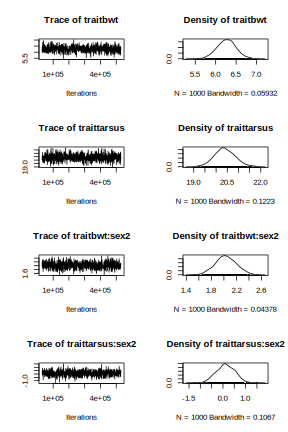
\includegraphics{wam_tuto_files/figure-latex/unnamed-chunk-97-1.pdf}

\begin{Shaded}
\begin{Highlighting}[]
\CommentTok{\#}
\end{Highlighting}
\end{Shaded}

Here, some simple code to plot the genetic correlation.

\begin{Shaded}
\begin{Highlighting}[]
\KeywordTok{plot}\NormalTok{(BLUP.tarsus }\OperatorTok{\textasciitilde{}}\StringTok{ }\NormalTok{BLUP.btw, BLUPS, }\DataTypeTok{xlab =} \StringTok{""}\NormalTok{, }\DataTypeTok{ylab =} \StringTok{""}\NormalTok{, }\DataTypeTok{las =} \FloatTok{1.2}\NormalTok{, }\DataTypeTok{bty =} \StringTok{"o"}\NormalTok{, }\DataTypeTok{col =} \StringTok{"white"}\NormalTok{)}
\KeywordTok{arrows}\NormalTok{(}\DataTypeTok{x0 =}\NormalTok{ BLUPS}\OperatorTok{$}\NormalTok{BLUP.btw, }\DataTypeTok{y0 =}\NormalTok{ BLUPS}\OperatorTok{$}\NormalTok{BLUP.tarsus }\OperatorTok{{-}}\StringTok{ }\NormalTok{BLUPS}\OperatorTok{$}\NormalTok{SE.tarsus, }\DataTypeTok{x1 =}\NormalTok{ BLUPS}\OperatorTok{$}\NormalTok{BLUP.btw, }\DataTypeTok{y1 =}\NormalTok{ BLUPS}\OperatorTok{$}\NormalTok{BLUP.tarsus }\OperatorTok{+}\StringTok{ }\NormalTok{BLUPS}\OperatorTok{$}\NormalTok{SE.tarsus, }\DataTypeTok{col =} \StringTok{"black"}\NormalTok{, }\DataTypeTok{code =} \DecValTok{3}\NormalTok{, }\DataTypeTok{angle =} \DecValTok{90}\NormalTok{, }\DataTypeTok{length =} \DecValTok{0}\NormalTok{)}
\KeywordTok{arrows}\NormalTok{(}\DataTypeTok{x0 =}\NormalTok{ BLUPS}\OperatorTok{$}\NormalTok{BLUP.btw }\OperatorTok{{-}}\StringTok{ }\NormalTok{BLUPS}\OperatorTok{$}\NormalTok{SE.btw, }\DataTypeTok{y0 =}\NormalTok{ BLUPS}\OperatorTok{$}\NormalTok{BLUP.tarsus, }\DataTypeTok{x1 =}\NormalTok{ BLUPS}\OperatorTok{$}\NormalTok{BLUP.btw }\OperatorTok{+}\StringTok{ }\NormalTok{BLUPS}\OperatorTok{$}\NormalTok{SE.btw, }\DataTypeTok{y1 =}\NormalTok{ BLUPS}\OperatorTok{$}\NormalTok{BLUP.tarsus, }\DataTypeTok{col =} \StringTok{"black"}\NormalTok{, }\DataTypeTok{code =} \DecValTok{3}\NormalTok{, }\DataTypeTok{angle =} \DecValTok{90}\NormalTok{, }\DataTypeTok{length =} \DecValTok{0}\NormalTok{)}
\KeywordTok{points}\NormalTok{(BLUP.tarsus }\OperatorTok{\textasciitilde{}}\StringTok{ }\NormalTok{BLUP.btw, BLUPS, }\DataTypeTok{pch =} \DecValTok{16}\NormalTok{, }\DataTypeTok{col =} \StringTok{"red"}\NormalTok{, }\DataTypeTok{cex =} \FloatTok{1.5}\NormalTok{)}
\KeywordTok{points}\NormalTok{(BLUP.tarsus }\OperatorTok{\textasciitilde{}}\StringTok{ }\NormalTok{BLUP.btw, BLUPS, }\DataTypeTok{pch =} \DecValTok{1}\NormalTok{, }\DataTypeTok{col =} \KeywordTok{rgb}\NormalTok{(}\DecValTok{0}\NormalTok{, }\DecValTok{0}\NormalTok{, }\DecValTok{0}\NormalTok{, }\FloatTok{0.3}\NormalTok{), }\DataTypeTok{cex =} \KeywordTok{c}\NormalTok{(}\FloatTok{1.5}\NormalTok{))}
\KeywordTok{mtext}\NormalTok{(}\StringTok{"btw (BV±SE)"}\NormalTok{, }\DataTypeTok{side =} \DecValTok{1}\NormalTok{, }\DataTypeTok{line =} \FloatTok{2.4}\NormalTok{)}
\KeywordTok{mtext}\NormalTok{(}\StringTok{"tarsus (BV±SE)"}\NormalTok{, }\DataTypeTok{side =} \DecValTok{2}\NormalTok{, }\DataTypeTok{line =} \DecValTok{2}\NormalTok{, }\DataTypeTok{las =} \DecValTok{3}\NormalTok{)}
\KeywordTok{mtext}\NormalTok{(}\KeywordTok{expression}\NormalTok{(}\KeywordTok{paste}\NormalTok{(}\KeywordTok{italic}\NormalTok{(r)[A], }\StringTok{" = 0.7353065 ±  0.1094838"}\NormalTok{)), }\DataTypeTok{side =} \DecValTok{1}\NormalTok{, }\DataTypeTok{line =} \DecValTok{{-}1}\NormalTok{, }\DataTypeTok{adj =} \FloatTok{0.95}\NormalTok{, }\DataTypeTok{cex =} \FloatTok{0.9}\NormalTok{)}
\end{Highlighting}
\end{Shaded}

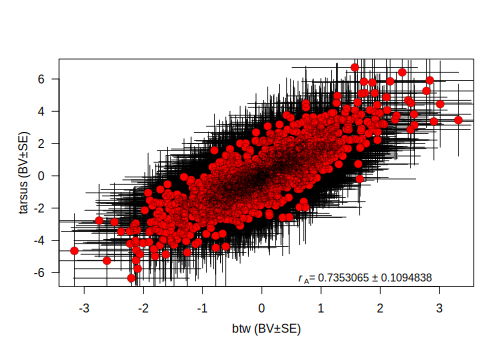
\includegraphics{wam_tuto_files/figure-latex/unnamed-chunk-98-1.pdf}

\hypertarget{partitionning-covariance-between-groups}{%
\subsection{Partitionning (co)variance between groups}\label{partitionning-covariance-between-groups}}

Similar to the univariate model, it is possible to partition the variance and also the covariance between different groups within the dataset. Here, we can estimate sex-specific genetic correlation.
Note, to partition a correlation, it is require to have important sample size within each group. For this example, we simplify the model !

\begin{Shaded}
\begin{Highlighting}[]
\NormalTok{gryphon \textless{}{-}}\StringTok{ }\NormalTok{gryphon[}\KeywordTok{order}\NormalTok{(gryphon}\OperatorTok{$}\NormalTok{sex), ]}
\NormalTok{model\_sex \textless{}{-}}\StringTok{ }\KeywordTok{asreml}\NormalTok{(}
  \DataTypeTok{fixed =} \KeywordTok{cbind}\NormalTok{(bwt, tarsus) }\OperatorTok{\textasciitilde{}}\StringTok{ }\NormalTok{trait }\OperatorTok{+}\StringTok{ }\KeywordTok{at}\NormalTok{(trait)}\OperatorTok{:}\NormalTok{sex,}
  \DataTypeTok{random =} \OperatorTok{\textasciitilde{}}\StringTok{ }\KeywordTok{at}\NormalTok{(sex)}\OperatorTok{:}\KeywordTok{us}\NormalTok{(trait, }\DataTypeTok{init =} \KeywordTok{c}\NormalTok{(}\DecValTok{1}\NormalTok{, }\FloatTok{0.1}\NormalTok{, }\DecValTok{1}\NormalTok{))}\OperatorTok{:}\KeywordTok{vm}\NormalTok{(animal, ainv) }\OperatorTok{+}
\StringTok{    }\KeywordTok{us}\NormalTok{(trait, }\DataTypeTok{init =} \KeywordTok{c}\NormalTok{(}\DecValTok{1}\NormalTok{, }\FloatTok{0.1}\NormalTok{, }\DecValTok{1}\NormalTok{))}\OperatorTok{:}\NormalTok{byear }\OperatorTok{+}
\StringTok{    }\KeywordTok{us}\NormalTok{(trait, }\DataTypeTok{init =} \KeywordTok{c}\NormalTok{(}\DecValTok{1}\NormalTok{, }\FloatTok{0.1}\NormalTok{, }\DecValTok{1}\NormalTok{))}\OperatorTok{:}\NormalTok{mother,}
  \DataTypeTok{residual =} \OperatorTok{\textasciitilde{}}\StringTok{ }\KeywordTok{dsum}\NormalTok{(}\OperatorTok{\textasciitilde{}}\StringTok{ }\KeywordTok{id}\NormalTok{(units)}\OperatorTok{:}\KeywordTok{us}\NormalTok{(trait) }\OperatorTok{|}\StringTok{ }\NormalTok{sex),}
  \DataTypeTok{data =}\NormalTok{ gryphon,}
  \DataTypeTok{na.action =} \KeywordTok{na.method}\NormalTok{(}\DataTypeTok{x =} \StringTok{"include"}\NormalTok{, }\DataTypeTok{y =} \StringTok{"include"}\NormalTok{),}
  \DataTypeTok{maxit =} \DecValTok{20}
\NormalTok{)}
\end{Highlighting}
\end{Shaded}

\begin{verbatim}
## Multi-section model using the sigma parameterization.
## ASReml 4.1.0 Sat Apr 30 11:10:30 2022
##           LogLik        Sigma2     DF     wall    cpu
##  1     -2522.729           1.0   1807 11:10:30    0.1 (1 restrained)
\end{verbatim}

\begin{verbatim}
## Warning in asreml(fixed = cbind(bwt, tarsus) ~ trait + at(trait):sex, random
## = ~at(sex):us(trait, : US updates modified 1 times in iteration 2 to remain
## positive definite.
\end{verbatim}

\begin{verbatim}
##  2     -2459.512           1.0   1807 11:10:30    0.1 (3 restrained)
##  3     -2408.940           1.0   1807 11:10:30    0.1
##  4     -2392.691           1.0   1807 11:10:30    0.1
##  5     -2388.962           1.0   1807 11:10:30    0.1
##  6     -2388.743           1.0   1807 11:10:30    0.1
##  7     -2388.736           1.0   1807 11:10:30    0.1
##  8     -2388.736           1.0   1807 11:10:30    0.1
\end{verbatim}

\begin{verbatim}
## Warning in asreml(fixed = cbind(bwt, tarsus) ~ trait + at(trait):sex, random =
## ~at(sex):us(trait, : US variance structures were modified in 1 instances to make
## them positive definite
\end{verbatim}

\begin{Shaded}
\begin{Highlighting}[]
\NormalTok{model\_sex \textless{}{-}}\StringTok{ }\KeywordTok{update}\NormalTok{(model\_sex)}
\end{Highlighting}
\end{Shaded}

\begin{verbatim}
## Multi-section model using the sigma parameterization.
## ASReml 4.1.0 Sat Apr 30 11:10:31 2022
##           LogLik        Sigma2     DF     wall    cpu
##  1     -2388.736           1.0   1807 11:10:31    0.1
##  2     -2388.736           1.0   1807 11:10:31    0.1
\end{verbatim}

\begin{Shaded}
\begin{Highlighting}[]
\KeywordTok{summary}\NormalTok{(model\_sex)}\OperatorTok{$}\NormalTok{varcomp}
\end{Highlighting}
\end{Shaded}

\begin{verbatim}
##                                                        component std.error
## trait:byear!trait_bwt:bwt                              0.9858478 0.2863878
## trait:byear!trait_tarsus:bwt                           0.1525063 0.4334263
## trait:byear!trait_tarsus:tarsus                        3.9981983 1.2798747
## trait:mother!trait_bwt:bwt                             1.3312734 0.2484444
## trait:mother!trait_tarsus:bwt                         -1.6174228 0.4283851
## trait:mother!trait_tarsus:tarsus                       4.7542338 1.3546517
## at(sex, 1):trait:vm(animal, ainv)!trait_bwt:bwt        1.3402853 0.5670773
## at(sex, 1):trait:vm(animal, ainv)!trait_tarsus:bwt     2.3608392 1.1348473
## at(sex, 1):trait:vm(animal, ainv)!trait_tarsus:tarsus  6.0625993 3.1304394
## at(sex, 2):trait:vm(animal, ainv)!trait_bwt:bwt        1.8645998 0.8888206
## at(sex, 2):trait:vm(animal, ainv)!trait_tarsus:bwt     5.0954811 2.0684729
## at(sex, 2):trait:vm(animal, ainv)!trait_tarsus:tarsus 14.9771870 6.4479787
## sex_1!R                                                1.0000000        NA
## sex_1!trait_bwt:bwt                                    2.3079850 0.5015651
## sex_1!trait_tarsus:bwt                                 4.4287898 1.0376370
## sex_1!trait_tarsus:tarsus                             13.4857819 2.9284922
## sex_2!R                                                1.0000000        NA
## sex_2!trait_bwt:bwt                                    1.7956612 0.7549779
## sex_2!trait_tarsus:bwt                                 2.6340448 1.7685804
## sex_2!trait_tarsus:tarsus                              9.6094528 5.4917853
##                                                          z.ratio bound %ch
## trait:byear!trait_bwt:bwt                              3.4423530     P   0
## trait:byear!trait_tarsus:bwt                           0.3518622     P   0
## trait:byear!trait_tarsus:tarsus                        3.1238982     P   0
## trait:mother!trait_bwt:bwt                             5.3584371     P   0
## trait:mother!trait_tarsus:bwt                         -3.7756279     P   0
## trait:mother!trait_tarsus:tarsus                       3.5095618     P   0
## at(sex, 1):trait:vm(animal, ainv)!trait_bwt:bwt        2.3634965     P   0
## at(sex, 1):trait:vm(animal, ainv)!trait_tarsus:bwt     2.0803144     P   0
## at(sex, 1):trait:vm(animal, ainv)!trait_tarsus:tarsus  1.9366608     P   0
## at(sex, 2):trait:vm(animal, ainv)!trait_bwt:bwt        2.0978361     P   0
## at(sex, 2):trait:vm(animal, ainv)!trait_tarsus:bwt     2.4634024     P   0
## at(sex, 2):trait:vm(animal, ainv)!trait_tarsus:tarsus  2.3227724     P   0
## sex_1!R                                                       NA     F   0
## sex_1!trait_bwt:bwt                                    4.6015657     P   0
## sex_1!trait_tarsus:bwt                                 4.2681493     P   0
## sex_1!trait_tarsus:tarsus                              4.6050257     P   0
## sex_2!R                                                       NA     F   0
## sex_2!trait_bwt:bwt                                    2.3784288     P   0
## sex_2!trait_tarsus:bwt                                 1.4893554     P   0
## sex_2!trait_tarsus:tarsus                              1.7497867     P   0
\end{verbatim}

we can estimate the different correlations using \texttt{vpredict}:

\begin{Shaded}
\begin{Highlighting}[]
\KeywordTok{vpredict}\NormalTok{(model\_sex, r\_byear }\OperatorTok{\textasciitilde{}}\StringTok{ }\NormalTok{V2 }\OperatorTok{/}\StringTok{ }\KeywordTok{sqrt}\NormalTok{(V1 }\OperatorTok{*}\StringTok{ }\NormalTok{V3))}
\end{Highlighting}
\end{Shaded}

\begin{verbatim}
##           Estimate       SE
## r_byear 0.07681584 0.213141
\end{verbatim}

\begin{Shaded}
\begin{Highlighting}[]
\KeywordTok{vpredict}\NormalTok{(model\_sex, r\_M }\OperatorTok{\textasciitilde{}}\StringTok{ }\NormalTok{V5 }\OperatorTok{/}\StringTok{ }\KeywordTok{sqrt}\NormalTok{(V4 }\OperatorTok{*}\StringTok{ }\NormalTok{V6))}
\end{Highlighting}
\end{Shaded}

\begin{verbatim}
##       Estimate       SE
## r_M -0.6429092 0.248944
\end{verbatim}

\begin{Shaded}
\begin{Highlighting}[]
\KeywordTok{vpredict}\NormalTok{(model\_sex, r\_A}\FloatTok{.1} \OperatorTok{\textasciitilde{}}\StringTok{ }\NormalTok{V8 }\OperatorTok{/}\StringTok{ }\KeywordTok{sqrt}\NormalTok{(V7 }\OperatorTok{*}\StringTok{ }\NormalTok{V9))}
\end{Highlighting}
\end{Shaded}

\begin{verbatim}
##        Estimate        SE
## r_A.1 0.8282059 0.1723596
\end{verbatim}

\begin{Shaded}
\begin{Highlighting}[]
\KeywordTok{vpredict}\NormalTok{(model\_sex, r\_A}\FloatTok{.2} \OperatorTok{\textasciitilde{}}\StringTok{ }\NormalTok{V11 }\OperatorTok{/}\StringTok{ }\KeywordTok{sqrt}\NormalTok{(V10 }\OperatorTok{*}\StringTok{ }\NormalTok{V12))}
\end{Highlighting}
\end{Shaded}

\begin{verbatim}
##        Estimate        SE
## r_A.2 0.9642225 0.1241668
\end{verbatim}

\begin{Shaded}
\begin{Highlighting}[]
\KeywordTok{vpredict}\NormalTok{(model\_sex, r\_res}\FloatTok{.1} \OperatorTok{\textasciitilde{}}\StringTok{ }\NormalTok{V15 }\OperatorTok{/}\StringTok{ }\KeywordTok{sqrt}\NormalTok{(V14 }\OperatorTok{*}\StringTok{ }\NormalTok{V16))}
\end{Highlighting}
\end{Shaded}

\begin{verbatim}
##          Estimate         SE
## r_res.1 0.7938355 0.07892634
\end{verbatim}

\begin{Shaded}
\begin{Highlighting}[]
\KeywordTok{vpredict}\NormalTok{(model\_sex, r\_res}\FloatTok{.2} \OperatorTok{\textasciitilde{}}\StringTok{ }\NormalTok{V19 }\OperatorTok{/}\StringTok{ }\KeywordTok{sqrt}\NormalTok{(V18 }\OperatorTok{*}\StringTok{ }\NormalTok{V20))}
\end{Highlighting}
\end{Shaded}

\begin{verbatim}
##          Estimate        SE
## r_res.2 0.6341057 0.1894837
\end{verbatim}

and the heritability too:

\begin{Shaded}
\begin{Highlighting}[]
\KeywordTok{vpredict}\NormalTok{(model\_sex, h2.bwt}\FloatTok{.1} \OperatorTok{\textasciitilde{}}\StringTok{ }\NormalTok{V7 }\OperatorTok{/}\StringTok{ }\NormalTok{(V1 }\OperatorTok{+}\StringTok{ }\NormalTok{V4 }\OperatorTok{+}\StringTok{ }\NormalTok{V7 }\OperatorTok{+}\StringTok{ }\NormalTok{V14))}
\end{Highlighting}
\end{Shaded}

\begin{verbatim}
##           Estimate         SE
## h2.bwt.1 0.2246768 0.09176827
\end{verbatim}

\begin{Shaded}
\begin{Highlighting}[]
\KeywordTok{vpredict}\NormalTok{(model\_sex, h2.bwt}\FloatTok{.2} \OperatorTok{\textasciitilde{}}\StringTok{ }\NormalTok{V10 }\OperatorTok{/}\StringTok{ }\NormalTok{(V1 }\OperatorTok{+}\StringTok{ }\NormalTok{V4 }\OperatorTok{+}\StringTok{ }\NormalTok{V10 }\OperatorTok{+}\StringTok{ }\NormalTok{V18))}
\end{Highlighting}
\end{Shaded}

\begin{verbatim}
##           Estimate        SE
## h2.bwt.2 0.3119425 0.1442547
\end{verbatim}

\begin{Shaded}
\begin{Highlighting}[]
\KeywordTok{vpredict}\NormalTok{(model\_sex, h2.tarsus}\FloatTok{.1} \OperatorTok{\textasciitilde{}}\StringTok{ }\NormalTok{V9 }\OperatorTok{/}\StringTok{ }\NormalTok{(V3 }\OperatorTok{+}\StringTok{ }\NormalTok{V6 }\OperatorTok{+}\StringTok{ }\NormalTok{V9 }\OperatorTok{+}\StringTok{ }\NormalTok{V16))}
\end{Highlighting}
\end{Shaded}

\begin{verbatim}
##             Estimate        SE
## h2.tarsus.1  0.21422 0.1070464
\end{verbatim}

\begin{Shaded}
\begin{Highlighting}[]
\KeywordTok{vpredict}\NormalTok{(model\_sex, h2.tarsus}\FloatTok{.2} \OperatorTok{\textasciitilde{}}\StringTok{ }\NormalTok{V12 }\OperatorTok{/}\StringTok{ }\NormalTok{(V3 }\OperatorTok{+}\StringTok{ }\NormalTok{V6 }\OperatorTok{+}\StringTok{ }\NormalTok{V12 }\OperatorTok{+}\StringTok{ }\NormalTok{V20))}
\end{Highlighting}
\end{Shaded}

\begin{verbatim}
##              Estimate        SE
## h2.tarsus.2 0.4492383 0.1833858
\end{verbatim}

Now we can look at the fixed effects parameters and assess their significance with a conditional Wald F-test:

\begin{Shaded}
\begin{Highlighting}[]
\KeywordTok{summary}\NormalTok{(model\_sex, }\DataTypeTok{coef =} \OtherTok{TRUE}\NormalTok{)}\OperatorTok{$}\NormalTok{coef.fi}
\KeywordTok{wald.asreml}\NormalTok{(model\_sex, }\DataTypeTok{denDF =} \StringTok{"default"}\NormalTok{, }\DataTypeTok{ssType =} \StringTok{"conditional"}\NormalTok{)}\OperatorTok{$}\NormalTok{Wald}
\end{Highlighting}
\end{Shaded}

\begin{verbatim}
##                           solution std error    z.ratio
## at(trait, tarsus):sex_1  0.0000000        NA         NA
## at(trait, tarsus):sex_2 -0.0554799 0.4758708 -0.1165861
## at(trait, bwt):sex_1     0.0000000        NA         NA
## at(trait, bwt):sex_2     1.9393688 0.1903239 10.1898321
## trait_bwt                6.3779149 0.2311766 27.5889321
## trait_tarsus            20.5838787 0.4942649 41.6454395
\end{verbatim}

\begin{verbatim}
## Multi-section model using the sigma parameterization.
## ASReml 4.1.0 Sat Apr 30 11:10:31 2022
##           LogLik        Sigma2     DF     wall    cpu
##  1     -2388.736           1.0   1807 11:10:31    0.1
##  2     -2388.736           1.0   1807 11:10:31    0.1
## Calculating denominator DF
\end{verbatim}

\begin{verbatim}
## 
##                       Df denDF   F.inc   F.con Margin      Pr
## trait                  2  44.8 1522.00 1522.00        0.00000
## at(trait, bwt):sex     1 137.5  220.90  103.80      B 0.00000
## at(trait, tarsus):sex  1 138.6    0.01    0.01      B 0.90737
\end{verbatim}

To assess the significant of the covariance, a LTR test can be done with a reduced model where a specific covariance can be fixed to 0 (for example the female covariance, following code).

\begin{Shaded}
\begin{Highlighting}[]
\NormalTok{model\_modif \textless{}{-}}\StringTok{ }\KeywordTok{update.asreml}\NormalTok{(model\_sex, }\DataTypeTok{start.values =}\NormalTok{ T)}
\NormalTok{G \textless{}{-}}\StringTok{ }\NormalTok{model\_modif}\OperatorTok{$}\NormalTok{vparameters[(}\DecValTok{1}\OperatorTok{:}\DecValTok{12}\NormalTok{), ]}
\NormalTok{G}\OperatorTok{$}\NormalTok{Constraint[(}\DecValTok{2}\NormalTok{)] \textless{}{-}}\StringTok{ "F"}
\NormalTok{G}\OperatorTok{$}\NormalTok{Value[(}\DecValTok{2}\NormalTok{)] \textless{}{-}}\StringTok{ }\DecValTok{0}
\CommentTok{\#}
\NormalTok{reduc.model\_sex \textless{}{-}}\StringTok{ }\KeywordTok{asreml}\NormalTok{(}
  \DataTypeTok{fixed =} \KeywordTok{cbind}\NormalTok{(bwt, tarsus) }\OperatorTok{\textasciitilde{}}\StringTok{ }\NormalTok{trait }\OperatorTok{+}\StringTok{ }\KeywordTok{at}\NormalTok{(trait)}\OperatorTok{:}\NormalTok{sex,}
  \DataTypeTok{random =} \OperatorTok{\textasciitilde{}}\StringTok{ }\KeywordTok{at}\NormalTok{(sex)}\OperatorTok{:}\KeywordTok{us}\NormalTok{(trait, }\DataTypeTok{init =} \KeywordTok{c}\NormalTok{(}\DecValTok{1}\NormalTok{, }\FloatTok{0.1}\NormalTok{, }\DecValTok{1}\NormalTok{))}\OperatorTok{:}\KeywordTok{vm}\NormalTok{(animal, ainv) }\OperatorTok{+}
\StringTok{    }\KeywordTok{us}\NormalTok{(trait, }\DataTypeTok{init =} \KeywordTok{c}\NormalTok{(}\DecValTok{1}\NormalTok{, }\FloatTok{0.1}\NormalTok{, }\DecValTok{1}\NormalTok{))}\OperatorTok{:}\NormalTok{byear }\OperatorTok{+}
\StringTok{    }\KeywordTok{us}\NormalTok{(trait, }\DataTypeTok{init =} \KeywordTok{c}\NormalTok{(}\DecValTok{1}\NormalTok{, }\FloatTok{0.1}\NormalTok{, }\DecValTok{1}\NormalTok{))}\OperatorTok{:}\NormalTok{mother,}
  \DataTypeTok{residual =} \OperatorTok{\textasciitilde{}}\StringTok{ }\KeywordTok{dsum}\NormalTok{(}\OperatorTok{\textasciitilde{}}\StringTok{ }\KeywordTok{id}\NormalTok{(units)}\OperatorTok{:}\KeywordTok{us}\NormalTok{(trait) }\OperatorTok{|}\StringTok{ }\NormalTok{sex),}
  \DataTypeTok{data =}\NormalTok{ gryphon,}
  \DataTypeTok{na.action =} \KeywordTok{na.method}\NormalTok{(}\DataTypeTok{x =} \StringTok{"include"}\NormalTok{, }\DataTypeTok{y =} \StringTok{"include"}\NormalTok{),}
  \DataTypeTok{maxit =} \DecValTok{20}\NormalTok{,}
  \DataTypeTok{G.param =}\NormalTok{ G}
\NormalTok{)}
\end{Highlighting}
\end{Shaded}

\begin{verbatim}
## Multi-section model using the sigma parameterization.
## ASReml 4.1.0 Sat Apr 30 11:10:32 2022
\end{verbatim}

\begin{verbatim}
## Warning in asreml(fixed = cbind(bwt, tarsus) ~ trait + at(trait):sex, random
## = ~at(sex):us(trait, : US updates modified 1 times in iteration 1 to remain
## positive definite.
\end{verbatim}

\begin{verbatim}
##           LogLik        Sigma2     DF     wall    cpu
##  1     -2474.972           1.0   1807 11:10:32    0.1 (3 restrained)
##  2     -2406.283           1.0   1807 11:10:32    0.1
##  3     -2394.010           1.0   1807 11:10:32    0.1
##  4     -2391.718           1.0   1807 11:10:33    0.1
##  5     -2391.480           1.0   1807 11:10:33    0.1
##  6     -2391.477           1.0   1807 11:10:33    0.1
\end{verbatim}

\begin{verbatim}
## Warning in asreml(fixed = cbind(bwt, tarsus) ~ trait + at(trait):sex, random =
## ~at(sex):us(trait, : US variance structures were modified in 1 instances to make
## them positive definite
\end{verbatim}

\begin{Shaded}
\begin{Highlighting}[]
\NormalTok{reduc.model\_sex \textless{}{-}}\StringTok{ }\KeywordTok{update}\NormalTok{(reduc.model\_sex)}
\end{Highlighting}
\end{Shaded}

\begin{verbatim}
## Multi-section model using the sigma parameterization.
## ASReml 4.1.0 Sat Apr 30 11:10:33 2022
##           LogLik        Sigma2     DF     wall    cpu
##  1     -2391.476           1.0   1807 11:10:33    0.2
##  2     -2391.476           1.0   1807 11:10:33    0.1
\end{verbatim}

\begin{Shaded}
\begin{Highlighting}[]
\KeywordTok{summary}\NormalTok{(reduc.model\_sex)}\OperatorTok{$}\NormalTok{varcomp}
\end{Highlighting}
\end{Shaded}

\begin{verbatim}
##                                                        component std.error
## trait:byear!trait_bwt:bwt                              0.9794331 0.2848997
## trait:byear!trait_tarsus:bwt                           0.1428995 0.4322719
## trait:byear!trait_tarsus:tarsus                        4.0021595 1.2818624
## trait:mother!trait_bwt:bwt                             1.4956509 0.2568074
## trait:mother!trait_tarsus:bwt                         -1.2460057 0.4438357
## trait:mother!trait_tarsus:tarsus                       5.3945609 1.4035705
## at(sex, 1):trait:vm(animal, ainv)!trait_bwt:bwt        0.5265716 0.3579555
## at(sex, 1):trait:vm(animal, ainv)!trait_tarsus:bwt     0.0000000        NA
## at(sex, 1):trait:vm(animal, ainv)!trait_tarsus:tarsus  1.4223969 1.9103795
## at(sex, 2):trait:vm(animal, ainv)!trait_bwt:bwt        1.5835813 0.8671365
## at(sex, 2):trait:vm(animal, ainv)!trait_tarsus:bwt     4.4288714 2.0173971
## at(sex, 2):trait:vm(animal, ainv)!trait_tarsus:tarsus 12.9349047 6.2946996
## sex_1!R                                                1.0000000        NA
## sex_1!trait_bwt:bwt                                    2.9539767 0.4196755
## sex_1!trait_tarsus:bwt                                 6.3138301 0.6802598
## sex_1!trait_tarsus:tarsus                             17.3577089 2.4730547
## sex_2!R                                                1.0000000        NA
## sex_2!trait_bwt:bwt                                    1.9341439 0.7416691
## sex_2!trait_tarsus:bwt                                 2.9467290 1.7370018
## sex_2!trait_tarsus:tarsus                             10.7245912 5.4025888
##                                                          z.ratio bound %ch
## trait:byear!trait_bwt:bwt                              3.4378175     P   0
## trait:byear!trait_tarsus:bwt                           0.3305778     P   0
## trait:byear!trait_tarsus:tarsus                        3.1221444     P   0
## trait:mother!trait_bwt:bwt                             5.8240170     P   0
## trait:mother!trait_tarsus:bwt                         -2.8073580     P   0
## trait:mother!trait_tarsus:tarsus                       3.8434556     P   0
## at(sex, 1):trait:vm(animal, ainv)!trait_bwt:bwt        1.4710530     P   0
## at(sex, 1):trait:vm(animal, ainv)!trait_tarsus:bwt            NA     F  NA
## at(sex, 1):trait:vm(animal, ainv)!trait_tarsus:tarsus  0.7445625     P   0
## at(sex, 2):trait:vm(animal, ainv)!trait_bwt:bwt        1.8262193     P   0
## at(sex, 2):trait:vm(animal, ainv)!trait_tarsus:bwt     2.1953395     P   0
## at(sex, 2):trait:vm(animal, ainv)!trait_tarsus:tarsus  2.0548883     P   0
## sex_1!R                                                       NA     F   0
## sex_1!trait_bwt:bwt                                    7.0387165     P   0
## sex_1!trait_tarsus:bwt                                 9.2814981     P   0
## sex_1!trait_tarsus:tarsus                              7.0187323     P   0
## sex_2!R                                                       NA     F   0
## sex_2!trait_bwt:bwt                                    2.6078261     P   0
## sex_2!trait_tarsus:bwt                                 1.6964455     P   0
## sex_2!trait_tarsus:tarsus                              1.9850837     P   0
\end{verbatim}

\begin{Shaded}
\begin{Highlighting}[]
\DecValTok{2} \OperatorTok{*}\StringTok{ }\NormalTok{(model\_sex}\OperatorTok{$}\NormalTok{loglik }\OperatorTok{{-}}\StringTok{ }\NormalTok{reduc.model\_sex}\OperatorTok{$}\NormalTok{loglik)}
\end{Highlighting}
\end{Shaded}

\begin{verbatim}
## [1] 5.481033
\end{verbatim}

\begin{Shaded}
\begin{Highlighting}[]
\DecValTok{1} \OperatorTok{{-}}\StringTok{ }\KeywordTok{pchisq}\NormalTok{(}\DecValTok{2} \OperatorTok{*}\StringTok{ }\NormalTok{(model\_sex}\OperatorTok{$}\NormalTok{loglik }\OperatorTok{{-}}\StringTok{ }\NormalTok{reduc.model\_sex}\OperatorTok{$}\NormalTok{loglik), }\DataTypeTok{df =} \DecValTok{1}\NormalTok{)}
\end{Highlighting}
\end{Shaded}

\begin{verbatim}
## [1] 0.0192239
\end{verbatim}

In addition, it is also possible to test if sexes has significant differences with another reduced model where both covariance are fixed to their average values.

\begin{Shaded}
\begin{Highlighting}[]
\CommentTok{\# code provided as an example for the moment since the model cannot run on this data}
\NormalTok{model\_modif \textless{}{-}}\StringTok{ }\KeywordTok{update.asreml}\NormalTok{(model\_sex, }\DataTypeTok{start.values =}\NormalTok{ T)}
\NormalTok{G \textless{}{-}}\StringTok{ }\NormalTok{model\_modif}\OperatorTok{$}\NormalTok{vparameters[(}\DecValTok{1}\OperatorTok{:}\DecValTok{12}\NormalTok{), ]}
\NormalTok{G}\OperatorTok{$}\NormalTok{fac \textless{}{-}}\StringTok{ }\KeywordTok{factor}\NormalTok{(}\KeywordTok{c}\NormalTok{(}
  \DecValTok{1}\NormalTok{, }\DecValTok{2}\NormalTok{, }\DecValTok{3}\NormalTok{, }\DecValTok{4}\NormalTok{, }\DecValTok{2}\NormalTok{, }\DecValTok{6}\NormalTok{, }\CommentTok{\# Additive genetic matrix  2 =5}
  \DecValTok{7}\NormalTok{, }\DecValTok{8}\NormalTok{, }\DecValTok{9}\NormalTok{, }\CommentTok{\# byear  matrix}
  \DecValTok{10}\NormalTok{, }\DecValTok{11}\NormalTok{, }\DecValTok{12}
\NormalTok{)) }\CommentTok{\# mother matrix}
\NormalTok{Modif \textless{}{-}}\StringTok{ }\KeywordTok{vcm.lm}\NormalTok{(}\OperatorTok{\textasciitilde{}}\NormalTok{fac, }\DataTypeTok{data =}\NormalTok{ G)}
\KeywordTok{attr}\NormalTok{(Modif, }\StringTok{"assign"}\NormalTok{) \textless{}{-}}\StringTok{ }\OtherTok{NULL}
\KeywordTok{attr}\NormalTok{(Modif, }\StringTok{"contrasts"}\NormalTok{) \textless{}{-}}\StringTok{ }\OtherTok{NULL}
\CommentTok{\#}
\NormalTok{reduc.model\_sex\_}\DecValTok{2}\NormalTok{ \textless{}{-}}\StringTok{ }\KeywordTok{asreml}\NormalTok{(}
  \DataTypeTok{fixed =} \KeywordTok{cbind}\NormalTok{(bwt, tarsus) }\OperatorTok{\textasciitilde{}}\StringTok{ }\NormalTok{trait }\OperatorTok{+}\StringTok{ }\KeywordTok{at}\NormalTok{(trait)}\OperatorTok{:}\NormalTok{sex,}
  \DataTypeTok{random =} \OperatorTok{\textasciitilde{}}\StringTok{ }\KeywordTok{at}\NormalTok{(sex)}\OperatorTok{:}\KeywordTok{us}\NormalTok{(trait, }\DataTypeTok{init =} \KeywordTok{c}\NormalTok{(}\DecValTok{1}\NormalTok{, }\FloatTok{0.1}\NormalTok{, }\DecValTok{1}\NormalTok{))}\OperatorTok{:}\KeywordTok{vm}\NormalTok{(animal, ainv) }\OperatorTok{+}
\StringTok{    }\KeywordTok{us}\NormalTok{(trait, }\DataTypeTok{init =} \KeywordTok{c}\NormalTok{(}\DecValTok{1}\NormalTok{, }\FloatTok{0.1}\NormalTok{, }\DecValTok{1}\NormalTok{))}\OperatorTok{:}\NormalTok{byear }\OperatorTok{+}
\StringTok{    }\KeywordTok{us}\NormalTok{(trait, }\DataTypeTok{init =} \KeywordTok{c}\NormalTok{(}\DecValTok{1}\NormalTok{, }\FloatTok{0.1}\NormalTok{, }\DecValTok{1}\NormalTok{))}\OperatorTok{:}\NormalTok{mother,}
  \DataTypeTok{residual =} \OperatorTok{\textasciitilde{}}\StringTok{ }\KeywordTok{dsum}\NormalTok{(}\OperatorTok{\textasciitilde{}}\StringTok{ }\KeywordTok{id}\NormalTok{(units)}\OperatorTok{:}\KeywordTok{us}\NormalTok{(trait) }\OperatorTok{|}\StringTok{ }\NormalTok{sex),}
  \DataTypeTok{data =}\NormalTok{ gryphon,}
  \DataTypeTok{na.action =} \KeywordTok{na.method}\NormalTok{(}\DataTypeTok{x =} \StringTok{"include"}\NormalTok{, }\DataTypeTok{y =} \StringTok{"include"}\NormalTok{),}
  \DataTypeTok{maxit =} \DecValTok{20}\NormalTok{,}
  \DataTypeTok{G.param =}\NormalTok{ G, }\DataTypeTok{vcm =}\NormalTok{ Modif}
\NormalTok{)}
\NormalTok{reduc.model\_sex\_}\DecValTok{2}\NormalTok{ \textless{}{-}}\StringTok{ }\KeywordTok{update}\NormalTok{(reduc.model\_sex\_}\DecValTok{2}\NormalTok{)}
\KeywordTok{summary}\NormalTok{(reduc.model\_sex\_}\DecValTok{2}\NormalTok{)}\OperatorTok{$}\NormalTok{varcomp}



\DecValTok{2} \OperatorTok{*}\StringTok{ }\NormalTok{(model\_sex}\OperatorTok{$}\NormalTok{loglik }\OperatorTok{{-}}\StringTok{ }\NormalTok{reduc.model\_sex\_}\DecValTok{2}\OperatorTok{$}\NormalTok{loglik)}
\DecValTok{1} \OperatorTok{{-}}\StringTok{ }\KeywordTok{pchisq}\NormalTok{(}\DecValTok{2} \OperatorTok{*}\StringTok{ }\NormalTok{(model\_sex}\OperatorTok{$}\NormalTok{loglik }\OperatorTok{{-}}\StringTok{ }\NormalTok{reduc.model\_sex\_}\DecValTok{2}\OperatorTok{$}\NormalTok{loglik), }\DataTypeTok{df =} \DecValTok{2}\NormalTok{)}
\end{Highlighting}
\end{Shaded}

Here a plot to visualize the overlaps of covariances.

\begin{Shaded}
\begin{Highlighting}[]
\NormalTok{genetic.correlation.F \textless{}{-}}\StringTok{ }\KeywordTok{vpredict}\NormalTok{(model\_sex, r\_A}\FloatTok{.1} \OperatorTok{\textasciitilde{}}\StringTok{ }\NormalTok{V8 }\OperatorTok{/}\StringTok{ }\KeywordTok{sqrt}\NormalTok{(V7 }\OperatorTok{*}\StringTok{ }\NormalTok{V9))}
\NormalTok{genetic.correlation.M \textless{}{-}}\StringTok{ }\KeywordTok{vpredict}\NormalTok{(model\_sex, r\_A}\FloatTok{.2} \OperatorTok{\textasciitilde{}}\StringTok{ }\NormalTok{V11 }\OperatorTok{/}\StringTok{ }\KeywordTok{sqrt}\NormalTok{(V10 }\OperatorTok{*}\StringTok{ }\NormalTok{V12))}
\NormalTok{residual.correlation.F \textless{}{-}}\StringTok{ }\KeywordTok{vpredict}\NormalTok{(model\_sex, r\_res}\FloatTok{.1} \OperatorTok{\textasciitilde{}}\StringTok{ }\NormalTok{V15 }\OperatorTok{/}\StringTok{ }\KeywordTok{sqrt}\NormalTok{(V14 }\OperatorTok{*}\StringTok{ }\NormalTok{V16))}
\NormalTok{residual.correlation.M \textless{}{-}}\StringTok{ }\KeywordTok{vpredict}\NormalTok{(model\_sex, r\_res}\FloatTok{.2} \OperatorTok{\textasciitilde{}}\StringTok{ }\NormalTok{V19 }\OperatorTok{/}\StringTok{ }\KeywordTok{sqrt}\NormalTok{(V18 }\OperatorTok{*}\StringTok{ }\NormalTok{V20))}
\NormalTok{cor.est \textless{}{-}}\StringTok{ }\KeywordTok{rbind}\NormalTok{(genetic.correlation.F, genetic.correlation.M, residual.correlation.F, residual.correlation.M)}

\KeywordTok{plot}\NormalTok{(}\KeywordTok{c}\NormalTok{(}\FloatTok{0.95}\NormalTok{, }\FloatTok{1.05}\NormalTok{, }\FloatTok{1.95}\NormalTok{, }\FloatTok{2.05}\NormalTok{) }\OperatorTok{\textasciitilde{}}\StringTok{ }\NormalTok{cor.est[, }\DecValTok{1}\NormalTok{], }\DataTypeTok{xlim =} \KeywordTok{c}\NormalTok{(}\DecValTok{0}\NormalTok{, }\FloatTok{1.5}\NormalTok{), }\DataTypeTok{ylim =} \KeywordTok{c}\NormalTok{(}\FloatTok{0.5}\NormalTok{, }\FloatTok{2.5}\NormalTok{), }\DataTypeTok{xlab =} \StringTok{""}\NormalTok{, }\DataTypeTok{ylab =} \StringTok{""}\NormalTok{, }\DataTypeTok{col =} \KeywordTok{c}\NormalTok{(}\StringTok{"red"}\NormalTok{, }\StringTok{"blue"}\NormalTok{), }\DataTypeTok{pch =} \KeywordTok{c}\NormalTok{(}\DecValTok{16}\NormalTok{, }\DecValTok{17}\NormalTok{), }\DataTypeTok{cex =} \DecValTok{2}\NormalTok{, }\DataTypeTok{yaxt =} \StringTok{"n"}\NormalTok{)}
\KeywordTok{arrows}\NormalTok{(}\DataTypeTok{y0 =} \FloatTok{0.95}\NormalTok{, }\DataTypeTok{x0 =}\NormalTok{ cor.est[}\DecValTok{1}\NormalTok{, }\DecValTok{1}\NormalTok{] }\OperatorTok{{-}}\StringTok{ }\NormalTok{cor.est[}\DecValTok{1}\NormalTok{, }\DecValTok{2}\NormalTok{], }\DataTypeTok{y1 =} \FloatTok{0.95}\NormalTok{, }\DataTypeTok{x1 =}\NormalTok{ cor.est[}\DecValTok{1}\NormalTok{, }\DecValTok{1}\NormalTok{] }\OperatorTok{+}\StringTok{ }\NormalTok{cor.est[}\DecValTok{1}\NormalTok{, }\DecValTok{2}\NormalTok{], }\DataTypeTok{code =} \DecValTok{3}\NormalTok{, }\DataTypeTok{angle =} \DecValTok{90}\NormalTok{, }\DataTypeTok{length =} \DecValTok{0}\NormalTok{, }\DataTypeTok{col =} \KeywordTok{c}\NormalTok{(}\StringTok{"red"}\NormalTok{), }\DataTypeTok{lwd =} \DecValTok{2}\NormalTok{)}
\KeywordTok{arrows}\NormalTok{(}\DataTypeTok{y0 =} \FloatTok{1.05}\NormalTok{, }\DataTypeTok{x0 =}\NormalTok{ cor.est[}\DecValTok{2}\NormalTok{, }\DecValTok{1}\NormalTok{] }\OperatorTok{{-}}\StringTok{ }\NormalTok{cor.est[}\DecValTok{2}\NormalTok{, }\DecValTok{2}\NormalTok{], }\DataTypeTok{y1 =} \FloatTok{1.05}\NormalTok{, }\DataTypeTok{x1 =}\NormalTok{ cor.est[}\DecValTok{2}\NormalTok{, }\DecValTok{1}\NormalTok{] }\OperatorTok{+}\StringTok{ }\NormalTok{cor.est[}\DecValTok{2}\NormalTok{, }\DecValTok{2}\NormalTok{], }\DataTypeTok{code =} \DecValTok{3}\NormalTok{, }\DataTypeTok{angle =} \DecValTok{90}\NormalTok{, }\DataTypeTok{length =} \DecValTok{0}\NormalTok{, }\DataTypeTok{col =} \KeywordTok{c}\NormalTok{(}\StringTok{"blue"}\NormalTok{), }\DataTypeTok{lwd =} \DecValTok{2}\NormalTok{)}
\KeywordTok{arrows}\NormalTok{(}\DataTypeTok{y0 =} \FloatTok{1.95}\NormalTok{, }\DataTypeTok{x0 =}\NormalTok{ cor.est[}\DecValTok{3}\NormalTok{, }\DecValTok{1}\NormalTok{] }\OperatorTok{{-}}\StringTok{ }\NormalTok{cor.est[}\DecValTok{3}\NormalTok{, }\DecValTok{2}\NormalTok{], }\DataTypeTok{y1 =} \FloatTok{1.95}\NormalTok{, }\DataTypeTok{x1 =}\NormalTok{ cor.est[}\DecValTok{3}\NormalTok{, }\DecValTok{1}\NormalTok{] }\OperatorTok{+}\StringTok{ }\NormalTok{cor.est[}\DecValTok{3}\NormalTok{, }\DecValTok{2}\NormalTok{], }\DataTypeTok{code =} \DecValTok{3}\NormalTok{, }\DataTypeTok{angle =} \DecValTok{90}\NormalTok{, }\DataTypeTok{length =} \DecValTok{0}\NormalTok{, }\DataTypeTok{col =} \KeywordTok{c}\NormalTok{(}\StringTok{"red"}\NormalTok{), }\DataTypeTok{lwd =} \DecValTok{2}\NormalTok{)}
\KeywordTok{arrows}\NormalTok{(}\DataTypeTok{y0 =} \FloatTok{2.05}\NormalTok{, }\DataTypeTok{x0 =}\NormalTok{ cor.est[}\DecValTok{4}\NormalTok{, }\DecValTok{1}\NormalTok{] }\OperatorTok{{-}}\StringTok{ }\NormalTok{cor.est[}\DecValTok{4}\NormalTok{, }\DecValTok{2}\NormalTok{], }\DataTypeTok{y1 =} \FloatTok{2.05}\NormalTok{, }\DataTypeTok{x1 =}\NormalTok{ cor.est[}\DecValTok{4}\NormalTok{, }\DecValTok{1}\NormalTok{] }\OperatorTok{+}\StringTok{ }\NormalTok{cor.est[}\DecValTok{4}\NormalTok{, }\DecValTok{2}\NormalTok{], }\DataTypeTok{code =} \DecValTok{3}\NormalTok{, }\DataTypeTok{angle =} \DecValTok{90}\NormalTok{, }\DataTypeTok{length =} \DecValTok{0}\NormalTok{, }\DataTypeTok{col =} \KeywordTok{c}\NormalTok{(}\StringTok{"blue"}\NormalTok{), }\DataTypeTok{lwd =} \DecValTok{2}\NormalTok{)}
\KeywordTok{mtext}\NormalTok{(}\StringTok{"Correlation (±CI)"}\NormalTok{, }\DataTypeTok{side =} \DecValTok{1}\NormalTok{, }\DataTypeTok{las =} \DecValTok{1}\NormalTok{, }\DataTypeTok{adj =} \FloatTok{0.4}\NormalTok{, }\DataTypeTok{line =} \DecValTok{3}\NormalTok{, }\DataTypeTok{cex =} \FloatTok{1.6}\NormalTok{)}
\KeywordTok{axis}\NormalTok{(}\DecValTok{2}\NormalTok{, }\DataTypeTok{at =} \DecValTok{1}\NormalTok{, }\DataTypeTok{labels =} \KeywordTok{c}\NormalTok{(}\StringTok{"genetic"}\NormalTok{), }\DataTypeTok{las =} \DecValTok{3}\NormalTok{, }\DataTypeTok{cex.axis =} \FloatTok{1.6}\NormalTok{)}
\KeywordTok{axis}\NormalTok{(}\DecValTok{2}\NormalTok{, }\DataTypeTok{at =} \DecValTok{2}\NormalTok{, }\DataTypeTok{labels =} \KeywordTok{c}\NormalTok{(}\StringTok{"residual"}\NormalTok{), }\DataTypeTok{las =} \DecValTok{3}\NormalTok{, }\DataTypeTok{cex.axis =} \FloatTok{1.6}\NormalTok{)}
\end{Highlighting}
\end{Shaded}

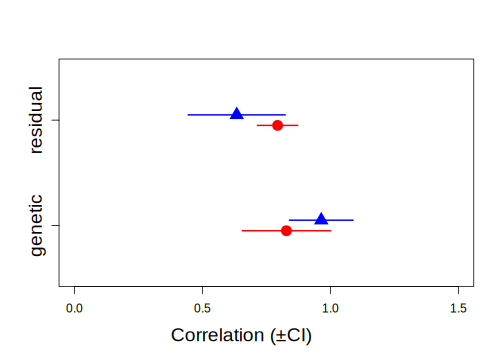
\includegraphics{wam_tuto_files/figure-latex/unnamed-chunk-106-1.pdf}

By using \texttt{corgh}, we can extract the BLUPs and plot the sex-specific correlation.

\begin{Shaded}
\begin{Highlighting}[]
\NormalTok{gryphon}\OperatorTok{$}\NormalTok{T1 \textless{}{-}}\StringTok{ }\NormalTok{gryphon}\OperatorTok{$}\NormalTok{bwt}
\NormalTok{gryphon}\OperatorTok{$}\NormalTok{T2 \textless{}{-}}\StringTok{ }\NormalTok{gryphon}\OperatorTok{$}\NormalTok{tarsus}
\CommentTok{\#\#\#}
\NormalTok{model\_sex \textless{}{-}}\StringTok{ }\KeywordTok{asreml}\NormalTok{(}
  \DataTypeTok{fixed =} \KeywordTok{cbind}\NormalTok{(T1, T2) }\OperatorTok{\textasciitilde{}}\StringTok{ }\NormalTok{trait }\OperatorTok{+}\StringTok{ }\KeywordTok{at}\NormalTok{(trait)}\OperatorTok{:}\NormalTok{sex,}
  \DataTypeTok{random =} \OperatorTok{\textasciitilde{}}\StringTok{ }\KeywordTok{at}\NormalTok{(sex)}\OperatorTok{:}\KeywordTok{corgh}\NormalTok{(trait, }\DataTypeTok{init =} \KeywordTok{c}\NormalTok{(}\FloatTok{0.1}\NormalTok{, }\DecValTok{1}\NormalTok{, }\DecValTok{1}\NormalTok{))}\OperatorTok{:}\KeywordTok{vm}\NormalTok{(animal, ainv) }\OperatorTok{+}
\StringTok{    }\KeywordTok{us}\NormalTok{(trait, }\DataTypeTok{init =} \KeywordTok{c}\NormalTok{(}\DecValTok{1}\NormalTok{, }\FloatTok{0.1}\NormalTok{, }\DecValTok{1}\NormalTok{))}\OperatorTok{:}\NormalTok{byear }\OperatorTok{+}
\StringTok{    }\KeywordTok{us}\NormalTok{(trait, }\DataTypeTok{init =} \KeywordTok{c}\NormalTok{(}\DecValTok{1}\NormalTok{, }\FloatTok{0.1}\NormalTok{, }\DecValTok{1}\NormalTok{))}\OperatorTok{:}\NormalTok{mother,}
  \DataTypeTok{residual =} \OperatorTok{\textasciitilde{}}\StringTok{ }\KeywordTok{dsum}\NormalTok{(}\OperatorTok{\textasciitilde{}}\StringTok{ }\KeywordTok{id}\NormalTok{(units)}\OperatorTok{:}\KeywordTok{us}\NormalTok{(trait) }\OperatorTok{|}\StringTok{ }\NormalTok{sex),}
  \DataTypeTok{data =}\NormalTok{ gryphon,}
  \DataTypeTok{na.action =} \KeywordTok{na.method}\NormalTok{(}\DataTypeTok{x =} \StringTok{"include"}\NormalTok{, }\DataTypeTok{y =} \StringTok{"include"}\NormalTok{),}
  \DataTypeTok{maxit =} \DecValTok{20}
\NormalTok{)}
\end{Highlighting}
\end{Shaded}

\begin{verbatim}
## Multi-section model using the sigma parameterization.
## ASReml 4.1.0 Sat Apr 30 11:10:33 2022
##           LogLik        Sigma2     DF     wall    cpu
##  1     -2522.729           1.0   1807 11:10:33    0.1 (2 restrained)
##  2     -2457.755           1.0   1807 11:10:33    0.1 (2 restrained)
##  3     -2407.462           1.0   1807 11:10:34    0.1 (2 restrained)
##  4     -2394.143           1.0   1807 11:10:34    0.1 (1 restrained)
##  5     -2389.368           1.0   1807 11:10:34    0.1
##  6     -2388.741           1.0   1807 11:10:34    0.1
##  7     -2388.736           1.0   1807 11:10:34    0.1
\end{verbatim}

\begin{Shaded}
\begin{Highlighting}[]
\NormalTok{model\_sex \textless{}{-}}\StringTok{ }\KeywordTok{update}\NormalTok{(model\_sex)}
\end{Highlighting}
\end{Shaded}

\begin{verbatim}
## Multi-section model using the sigma parameterization.
## ASReml 4.1.0 Sat Apr 30 11:10:34 2022
##           LogLik        Sigma2     DF     wall    cpu
##  1     -2388.736           1.0   1807 11:10:34    0.1
##  2     -2388.736           1.0   1807 11:10:34    0.1
\end{verbatim}

\begin{Shaded}
\begin{Highlighting}[]
\NormalTok{DvsS \textless{}{-}}\StringTok{ }\KeywordTok{data.frame}\NormalTok{(}
  \DataTypeTok{Trait =} \KeywordTok{rownames}\NormalTok{(model\_sex}\OperatorTok{$}\NormalTok{coefficients}\OperatorTok{$}\NormalTok{random),}
  \DataTypeTok{BLUP =}\NormalTok{ model\_sex}\OperatorTok{$}\NormalTok{coefficients}\OperatorTok{$}\NormalTok{random,}
  \DataTypeTok{SE =} \KeywordTok{sqrt}\NormalTok{(model\_sex}\OperatorTok{$}\NormalTok{vcoeff}\OperatorTok{$}\NormalTok{random }\OperatorTok{*}\StringTok{ }\NormalTok{model\_sex}\OperatorTok{$}\NormalTok{sigma2)}
\NormalTok{)}
\NormalTok{DvsS}\OperatorTok{$}\NormalTok{ID \textless{}{-}}\StringTok{ }\KeywordTok{substr}\NormalTok{(DvsS}\OperatorTok{$}\NormalTok{Trait, }\DecValTok{38}\NormalTok{, }\DecValTok{40}\NormalTok{)}
\NormalTok{DvsS}\OperatorTok{$}\NormalTok{TRAIT \textless{}{-}}\StringTok{ }\KeywordTok{substr}\NormalTok{(DvsS}\OperatorTok{$}\NormalTok{Trait, }\DecValTok{18}\NormalTok{, }\DecValTok{19}\NormalTok{)}
\NormalTok{DvsS}\OperatorTok{$}\NormalTok{SEX \textless{}{-}}\StringTok{ }\KeywordTok{substr}\NormalTok{(DvsS}\OperatorTok{$}\NormalTok{Trait, }\DecValTok{9}\NormalTok{, }\DecValTok{9}\NormalTok{)}
\NormalTok{DvsS \textless{}{-}}\StringTok{ }\NormalTok{DvsS[}\DecValTok{927}\OperatorTok{:}\DecValTok{6162}\NormalTok{, ] }\CommentTok{\# keep only row associated to animal}
\KeywordTok{summary}\NormalTok{(}\KeywordTok{factor}\NormalTok{(DvsS}\OperatorTok{$}\NormalTok{TRAIT)) }\CommentTok{\# 1309 each}
\end{Highlighting}
\end{Shaded}

\begin{verbatim}
##   T1   T2 
## 2618 2618
\end{verbatim}

\begin{Shaded}
\begin{Highlighting}[]
\CommentTok{\#}
\NormalTok{DvsS}\OperatorTok{$}\NormalTok{Trait \textless{}{-}}\StringTok{ }\OtherTok{NULL}
\KeywordTok{colnames}\NormalTok{(DvsS)[}\DecValTok{1}\NormalTok{] \textless{}{-}}\StringTok{ "BLUP"}
\NormalTok{BLUPS \textless{}{-}}\StringTok{ }\KeywordTok{reshape}\NormalTok{(DvsS, }\DataTypeTok{v.names =} \KeywordTok{c}\NormalTok{(}\StringTok{"BLUP"}\NormalTok{, }\StringTok{"SE"}\NormalTok{), }\DataTypeTok{idvar =} \KeywordTok{c}\NormalTok{(}\StringTok{"ID"}\NormalTok{, }\StringTok{"SEX"}\NormalTok{), }\DataTypeTok{timevar =} \StringTok{"TRAIT"}\NormalTok{, }\DataTypeTok{direction =} \StringTok{"wide"}\NormalTok{)}
\end{Highlighting}
\end{Shaded}

\begin{verbatim}
## Warning in reshapeWide(data, idvar = idvar, timevar = timevar, varying =
## varying, : multiple rows match for TRAIT=T1: first taken
\end{verbatim}

\begin{verbatim}
## Warning in reshapeWide(data, idvar = idvar, timevar = timevar, varying =
## varying, : multiple rows match for TRAIT=T2: first taken
\end{verbatim}

\begin{Shaded}
\begin{Highlighting}[]
\KeywordTok{row}\NormalTok{(BLUPS)}
\end{Highlighting}
\end{Shaded}

\begin{verbatim}
##         [,1] [,2] [,3] [,4] [,5] [,6]
##    [1,]    1    1    1    1    1    1
##    [2,]    2    2    2    2    2    2
##    [3,]    3    3    3    3    3    3
##    [4,]    4    4    4    4    4    4
##    [5,]    5    5    5    5    5    5
##    [6,]    6    6    6    6    6    6
##    [7,]    7    7    7    7    7    7
##    [8,]    8    8    8    8    8    8
##    [9,]    9    9    9    9    9    9
##   [10,]   10   10   10   10   10   10
##   [11,]   11   11   11   11   11   11
##   [12,]   12   12   12   12   12   12
##   [13,]   13   13   13   13   13   13
##   [14,]   14   14   14   14   14   14
##   [15,]   15   15   15   15   15   15
##   [16,]   16   16   16   16   16   16
##   [17,]   17   17   17   17   17   17
##   [18,]   18   18   18   18   18   18
##   [19,]   19   19   19   19   19   19
##   [20,]   20   20   20   20   20   20
##   [21,]   21   21   21   21   21   21
##   [22,]   22   22   22   22   22   22
##   [23,]   23   23   23   23   23   23
##   [24,]   24   24   24   24   24   24
##   [25,]   25   25   25   25   25   25
##   [26,]   26   26   26   26   26   26
##   [27,]   27   27   27   27   27   27
##   [28,]   28   28   28   28   28   28
##   [29,]   29   29   29   29   29   29
##   [30,]   30   30   30   30   30   30
##   [31,]   31   31   31   31   31   31
##   [32,]   32   32   32   32   32   32
##   [33,]   33   33   33   33   33   33
##   [34,]   34   34   34   34   34   34
##   [35,]   35   35   35   35   35   35
##   [36,]   36   36   36   36   36   36
##   [37,]   37   37   37   37   37   37
##   [38,]   38   38   38   38   38   38
##   [39,]   39   39   39   39   39   39
##   [40,]   40   40   40   40   40   40
##   [41,]   41   41   41   41   41   41
##   [42,]   42   42   42   42   42   42
##   [43,]   43   43   43   43   43   43
##   [44,]   44   44   44   44   44   44
##   [45,]   45   45   45   45   45   45
##   [46,]   46   46   46   46   46   46
##   [47,]   47   47   47   47   47   47
##   [48,]   48   48   48   48   48   48
##   [49,]   49   49   49   49   49   49
##   [50,]   50   50   50   50   50   50
##   [51,]   51   51   51   51   51   51
##   [52,]   52   52   52   52   52   52
##   [53,]   53   53   53   53   53   53
##   [54,]   54   54   54   54   54   54
##   [55,]   55   55   55   55   55   55
##   [56,]   56   56   56   56   56   56
##   [57,]   57   57   57   57   57   57
##   [58,]   58   58   58   58   58   58
##   [59,]   59   59   59   59   59   59
##   [60,]   60   60   60   60   60   60
##   [61,]   61   61   61   61   61   61
##   [62,]   62   62   62   62   62   62
##   [63,]   63   63   63   63   63   63
##   [64,]   64   64   64   64   64   64
##   [65,]   65   65   65   65   65   65
##   [66,]   66   66   66   66   66   66
##   [67,]   67   67   67   67   67   67
##   [68,]   68   68   68   68   68   68
##   [69,]   69   69   69   69   69   69
##   [70,]   70   70   70   70   70   70
##   [71,]   71   71   71   71   71   71
##   [72,]   72   72   72   72   72   72
##   [73,]   73   73   73   73   73   73
##   [74,]   74   74   74   74   74   74
##   [75,]   75   75   75   75   75   75
##   [76,]   76   76   76   76   76   76
##   [77,]   77   77   77   77   77   77
##   [78,]   78   78   78   78   78   78
##   [79,]   79   79   79   79   79   79
##   [80,]   80   80   80   80   80   80
##   [81,]   81   81   81   81   81   81
##   [82,]   82   82   82   82   82   82
##   [83,]   83   83   83   83   83   83
##   [84,]   84   84   84   84   84   84
##   [85,]   85   85   85   85   85   85
##   [86,]   86   86   86   86   86   86
##   [87,]   87   87   87   87   87   87
##   [88,]   88   88   88   88   88   88
##   [89,]   89   89   89   89   89   89
##   [90,]   90   90   90   90   90   90
##   [91,]   91   91   91   91   91   91
##   [92,]   92   92   92   92   92   92
##   [93,]   93   93   93   93   93   93
##   [94,]   94   94   94   94   94   94
##   [95,]   95   95   95   95   95   95
##   [96,]   96   96   96   96   96   96
##   [97,]   97   97   97   97   97   97
##   [98,]   98   98   98   98   98   98
##   [99,]   99   99   99   99   99   99
##  [100,]  100  100  100  100  100  100
##  [101,]  101  101  101  101  101  101
##  [102,]  102  102  102  102  102  102
##  [103,]  103  103  103  103  103  103
##  [104,]  104  104  104  104  104  104
##  [105,]  105  105  105  105  105  105
##  [106,]  106  106  106  106  106  106
##  [107,]  107  107  107  107  107  107
##  [108,]  108  108  108  108  108  108
##  [109,]  109  109  109  109  109  109
##  [110,]  110  110  110  110  110  110
##  [111,]  111  111  111  111  111  111
##  [112,]  112  112  112  112  112  112
##  [113,]  113  113  113  113  113  113
##  [114,]  114  114  114  114  114  114
##  [115,]  115  115  115  115  115  115
##  [116,]  116  116  116  116  116  116
##  [117,]  117  117  117  117  117  117
##  [118,]  118  118  118  118  118  118
##  [119,]  119  119  119  119  119  119
##  [120,]  120  120  120  120  120  120
##  [121,]  121  121  121  121  121  121
##  [122,]  122  122  122  122  122  122
##  [123,]  123  123  123  123  123  123
##  [124,]  124  124  124  124  124  124
##  [125,]  125  125  125  125  125  125
##  [126,]  126  126  126  126  126  126
##  [127,]  127  127  127  127  127  127
##  [128,]  128  128  128  128  128  128
##  [129,]  129  129  129  129  129  129
##  [130,]  130  130  130  130  130  130
##  [131,]  131  131  131  131  131  131
##  [132,]  132  132  132  132  132  132
##  [133,]  133  133  133  133  133  133
##  [134,]  134  134  134  134  134  134
##  [135,]  135  135  135  135  135  135
##  [136,]  136  136  136  136  136  136
##  [137,]  137  137  137  137  137  137
##  [138,]  138  138  138  138  138  138
##  [139,]  139  139  139  139  139  139
##  [140,]  140  140  140  140  140  140
##  [141,]  141  141  141  141  141  141
##  [142,]  142  142  142  142  142  142
##  [143,]  143  143  143  143  143  143
##  [144,]  144  144  144  144  144  144
##  [145,]  145  145  145  145  145  145
##  [146,]  146  146  146  146  146  146
##  [147,]  147  147  147  147  147  147
##  [148,]  148  148  148  148  148  148
##  [149,]  149  149  149  149  149  149
##  [150,]  150  150  150  150  150  150
##  [151,]  151  151  151  151  151  151
##  [152,]  152  152  152  152  152  152
##  [153,]  153  153  153  153  153  153
##  [154,]  154  154  154  154  154  154
##  [155,]  155  155  155  155  155  155
##  [156,]  156  156  156  156  156  156
##  [157,]  157  157  157  157  157  157
##  [158,]  158  158  158  158  158  158
##  [159,]  159  159  159  159  159  159
##  [160,]  160  160  160  160  160  160
##  [161,]  161  161  161  161  161  161
##  [162,]  162  162  162  162  162  162
##  [163,]  163  163  163  163  163  163
##  [164,]  164  164  164  164  164  164
##  [165,]  165  165  165  165  165  165
##  [166,]  166  166  166  166  166  166
##  [167,]  167  167  167  167  167  167
##  [168,]  168  168  168  168  168  168
##  [169,]  169  169  169  169  169  169
##  [170,]  170  170  170  170  170  170
##  [171,]  171  171  171  171  171  171
##  [172,]  172  172  172  172  172  172
##  [173,]  173  173  173  173  173  173
##  [174,]  174  174  174  174  174  174
##  [175,]  175  175  175  175  175  175
##  [176,]  176  176  176  176  176  176
##  [177,]  177  177  177  177  177  177
##  [178,]  178  178  178  178  178  178
##  [179,]  179  179  179  179  179  179
##  [180,]  180  180  180  180  180  180
##  [181,]  181  181  181  181  181  181
##  [182,]  182  182  182  182  182  182
##  [183,]  183  183  183  183  183  183
##  [184,]  184  184  184  184  184  184
##  [185,]  185  185  185  185  185  185
##  [186,]  186  186  186  186  186  186
##  [187,]  187  187  187  187  187  187
##  [188,]  188  188  188  188  188  188
##  [189,]  189  189  189  189  189  189
##  [190,]  190  190  190  190  190  190
##  [191,]  191  191  191  191  191  191
##  [192,]  192  192  192  192  192  192
##  [193,]  193  193  193  193  193  193
##  [194,]  194  194  194  194  194  194
##  [195,]  195  195  195  195  195  195
##  [196,]  196  196  196  196  196  196
##  [197,]  197  197  197  197  197  197
##  [198,]  198  198  198  198  198  198
##  [199,]  199  199  199  199  199  199
##  [200,]  200  200  200  200  200  200
##  [201,]  201  201  201  201  201  201
##  [202,]  202  202  202  202  202  202
##  [203,]  203  203  203  203  203  203
##  [204,]  204  204  204  204  204  204
##  [205,]  205  205  205  205  205  205
##  [206,]  206  206  206  206  206  206
##  [207,]  207  207  207  207  207  207
##  [208,]  208  208  208  208  208  208
##  [209,]  209  209  209  209  209  209
##  [210,]  210  210  210  210  210  210
##  [211,]  211  211  211  211  211  211
##  [212,]  212  212  212  212  212  212
##  [213,]  213  213  213  213  213  213
##  [214,]  214  214  214  214  214  214
##  [215,]  215  215  215  215  215  215
##  [216,]  216  216  216  216  216  216
##  [217,]  217  217  217  217  217  217
##  [218,]  218  218  218  218  218  218
##  [219,]  219  219  219  219  219  219
##  [220,]  220  220  220  220  220  220
##  [221,]  221  221  221  221  221  221
##  [222,]  222  222  222  222  222  222
##  [223,]  223  223  223  223  223  223
##  [224,]  224  224  224  224  224  224
##  [225,]  225  225  225  225  225  225
##  [226,]  226  226  226  226  226  226
##  [227,]  227  227  227  227  227  227
##  [228,]  228  228  228  228  228  228
##  [229,]  229  229  229  229  229  229
##  [230,]  230  230  230  230  230  230
##  [231,]  231  231  231  231  231  231
##  [232,]  232  232  232  232  232  232
##  [233,]  233  233  233  233  233  233
##  [234,]  234  234  234  234  234  234
##  [235,]  235  235  235  235  235  235
##  [236,]  236  236  236  236  236  236
##  [237,]  237  237  237  237  237  237
##  [238,]  238  238  238  238  238  238
##  [239,]  239  239  239  239  239  239
##  [240,]  240  240  240  240  240  240
##  [241,]  241  241  241  241  241  241
##  [242,]  242  242  242  242  242  242
##  [243,]  243  243  243  243  243  243
##  [244,]  244  244  244  244  244  244
##  [245,]  245  245  245  245  245  245
##  [246,]  246  246  246  246  246  246
##  [247,]  247  247  247  247  247  247
##  [248,]  248  248  248  248  248  248
##  [249,]  249  249  249  249  249  249
##  [250,]  250  250  250  250  250  250
##  [251,]  251  251  251  251  251  251
##  [252,]  252  252  252  252  252  252
##  [253,]  253  253  253  253  253  253
##  [254,]  254  254  254  254  254  254
##  [255,]  255  255  255  255  255  255
##  [256,]  256  256  256  256  256  256
##  [257,]  257  257  257  257  257  257
##  [258,]  258  258  258  258  258  258
##  [259,]  259  259  259  259  259  259
##  [260,]  260  260  260  260  260  260
##  [261,]  261  261  261  261  261  261
##  [262,]  262  262  262  262  262  262
##  [263,]  263  263  263  263  263  263
##  [264,]  264  264  264  264  264  264
##  [265,]  265  265  265  265  265  265
##  [266,]  266  266  266  266  266  266
##  [267,]  267  267  267  267  267  267
##  [268,]  268  268  268  268  268  268
##  [269,]  269  269  269  269  269  269
##  [270,]  270  270  270  270  270  270
##  [271,]  271  271  271  271  271  271
##  [272,]  272  272  272  272  272  272
##  [273,]  273  273  273  273  273  273
##  [274,]  274  274  274  274  274  274
##  [275,]  275  275  275  275  275  275
##  [276,]  276  276  276  276  276  276
##  [277,]  277  277  277  277  277  277
##  [278,]  278  278  278  278  278  278
##  [279,]  279  279  279  279  279  279
##  [280,]  280  280  280  280  280  280
##  [281,]  281  281  281  281  281  281
##  [282,]  282  282  282  282  282  282
##  [283,]  283  283  283  283  283  283
##  [284,]  284  284  284  284  284  284
##  [285,]  285  285  285  285  285  285
##  [286,]  286  286  286  286  286  286
##  [287,]  287  287  287  287  287  287
##  [288,]  288  288  288  288  288  288
##  [289,]  289  289  289  289  289  289
##  [290,]  290  290  290  290  290  290
##  [291,]  291  291  291  291  291  291
##  [292,]  292  292  292  292  292  292
##  [293,]  293  293  293  293  293  293
##  [294,]  294  294  294  294  294  294
##  [295,]  295  295  295  295  295  295
##  [296,]  296  296  296  296  296  296
##  [297,]  297  297  297  297  297  297
##  [298,]  298  298  298  298  298  298
##  [299,]  299  299  299  299  299  299
##  [300,]  300  300  300  300  300  300
##  [301,]  301  301  301  301  301  301
##  [302,]  302  302  302  302  302  302
##  [303,]  303  303  303  303  303  303
##  [304,]  304  304  304  304  304  304
##  [305,]  305  305  305  305  305  305
##  [306,]  306  306  306  306  306  306
##  [307,]  307  307  307  307  307  307
##  [308,]  308  308  308  308  308  308
##  [309,]  309  309  309  309  309  309
##  [310,]  310  310  310  310  310  310
##  [311,]  311  311  311  311  311  311
##  [312,]  312  312  312  312  312  312
##  [313,]  313  313  313  313  313  313
##  [314,]  314  314  314  314  314  314
##  [315,]  315  315  315  315  315  315
##  [316,]  316  316  316  316  316  316
##  [317,]  317  317  317  317  317  317
##  [318,]  318  318  318  318  318  318
##  [319,]  319  319  319  319  319  319
##  [320,]  320  320  320  320  320  320
##  [321,]  321  321  321  321  321  321
##  [322,]  322  322  322  322  322  322
##  [323,]  323  323  323  323  323  323
##  [324,]  324  324  324  324  324  324
##  [325,]  325  325  325  325  325  325
##  [326,]  326  326  326  326  326  326
##  [327,]  327  327  327  327  327  327
##  [328,]  328  328  328  328  328  328
##  [329,]  329  329  329  329  329  329
##  [330,]  330  330  330  330  330  330
##  [331,]  331  331  331  331  331  331
##  [332,]  332  332  332  332  332  332
##  [333,]  333  333  333  333  333  333
##  [334,]  334  334  334  334  334  334
##  [335,]  335  335  335  335  335  335
##  [336,]  336  336  336  336  336  336
##  [337,]  337  337  337  337  337  337
##  [338,]  338  338  338  338  338  338
##  [339,]  339  339  339  339  339  339
##  [340,]  340  340  340  340  340  340
##  [341,]  341  341  341  341  341  341
##  [342,]  342  342  342  342  342  342
##  [343,]  343  343  343  343  343  343
##  [344,]  344  344  344  344  344  344
##  [345,]  345  345  345  345  345  345
##  [346,]  346  346  346  346  346  346
##  [347,]  347  347  347  347  347  347
##  [348,]  348  348  348  348  348  348
##  [349,]  349  349  349  349  349  349
##  [350,]  350  350  350  350  350  350
##  [351,]  351  351  351  351  351  351
##  [352,]  352  352  352  352  352  352
##  [353,]  353  353  353  353  353  353
##  [354,]  354  354  354  354  354  354
##  [355,]  355  355  355  355  355  355
##  [356,]  356  356  356  356  356  356
##  [357,]  357  357  357  357  357  357
##  [358,]  358  358  358  358  358  358
##  [359,]  359  359  359  359  359  359
##  [360,]  360  360  360  360  360  360
##  [361,]  361  361  361  361  361  361
##  [362,]  362  362  362  362  362  362
##  [363,]  363  363  363  363  363  363
##  [364,]  364  364  364  364  364  364
##  [365,]  365  365  365  365  365  365
##  [366,]  366  366  366  366  366  366
##  [367,]  367  367  367  367  367  367
##  [368,]  368  368  368  368  368  368
##  [369,]  369  369  369  369  369  369
##  [370,]  370  370  370  370  370  370
##  [371,]  371  371  371  371  371  371
##  [372,]  372  372  372  372  372  372
##  [373,]  373  373  373  373  373  373
##  [374,]  374  374  374  374  374  374
##  [375,]  375  375  375  375  375  375
##  [376,]  376  376  376  376  376  376
##  [377,]  377  377  377  377  377  377
##  [378,]  378  378  378  378  378  378
##  [379,]  379  379  379  379  379  379
##  [380,]  380  380  380  380  380  380
##  [381,]  381  381  381  381  381  381
##  [382,]  382  382  382  382  382  382
##  [383,]  383  383  383  383  383  383
##  [384,]  384  384  384  384  384  384
##  [385,]  385  385  385  385  385  385
##  [386,]  386  386  386  386  386  386
##  [387,]  387  387  387  387  387  387
##  [388,]  388  388  388  388  388  388
##  [389,]  389  389  389  389  389  389
##  [390,]  390  390  390  390  390  390
##  [391,]  391  391  391  391  391  391
##  [392,]  392  392  392  392  392  392
##  [393,]  393  393  393  393  393  393
##  [394,]  394  394  394  394  394  394
##  [395,]  395  395  395  395  395  395
##  [396,]  396  396  396  396  396  396
##  [397,]  397  397  397  397  397  397
##  [398,]  398  398  398  398  398  398
##  [399,]  399  399  399  399  399  399
##  [400,]  400  400  400  400  400  400
##  [401,]  401  401  401  401  401  401
##  [402,]  402  402  402  402  402  402
##  [403,]  403  403  403  403  403  403
##  [404,]  404  404  404  404  404  404
##  [405,]  405  405  405  405  405  405
##  [406,]  406  406  406  406  406  406
##  [407,]  407  407  407  407  407  407
##  [408,]  408  408  408  408  408  408
##  [409,]  409  409  409  409  409  409
##  [410,]  410  410  410  410  410  410
##  [411,]  411  411  411  411  411  411
##  [412,]  412  412  412  412  412  412
##  [413,]  413  413  413  413  413  413
##  [414,]  414  414  414  414  414  414
##  [415,]  415  415  415  415  415  415
##  [416,]  416  416  416  416  416  416
##  [417,]  417  417  417  417  417  417
##  [418,]  418  418  418  418  418  418
##  [419,]  419  419  419  419  419  419
##  [420,]  420  420  420  420  420  420
##  [421,]  421  421  421  421  421  421
##  [422,]  422  422  422  422  422  422
##  [423,]  423  423  423  423  423  423
##  [424,]  424  424  424  424  424  424
##  [425,]  425  425  425  425  425  425
##  [426,]  426  426  426  426  426  426
##  [427,]  427  427  427  427  427  427
##  [428,]  428  428  428  428  428  428
##  [429,]  429  429  429  429  429  429
##  [430,]  430  430  430  430  430  430
##  [431,]  431  431  431  431  431  431
##  [432,]  432  432  432  432  432  432
##  [433,]  433  433  433  433  433  433
##  [434,]  434  434  434  434  434  434
##  [435,]  435  435  435  435  435  435
##  [436,]  436  436  436  436  436  436
##  [437,]  437  437  437  437  437  437
##  [438,]  438  438  438  438  438  438
##  [439,]  439  439  439  439  439  439
##  [440,]  440  440  440  440  440  440
##  [441,]  441  441  441  441  441  441
##  [442,]  442  442  442  442  442  442
##  [443,]  443  443  443  443  443  443
##  [444,]  444  444  444  444  444  444
##  [445,]  445  445  445  445  445  445
##  [446,]  446  446  446  446  446  446
##  [447,]  447  447  447  447  447  447
##  [448,]  448  448  448  448  448  448
##  [449,]  449  449  449  449  449  449
##  [450,]  450  450  450  450  450  450
##  [451,]  451  451  451  451  451  451
##  [452,]  452  452  452  452  452  452
##  [453,]  453  453  453  453  453  453
##  [454,]  454  454  454  454  454  454
##  [455,]  455  455  455  455  455  455
##  [456,]  456  456  456  456  456  456
##  [457,]  457  457  457  457  457  457
##  [458,]  458  458  458  458  458  458
##  [459,]  459  459  459  459  459  459
##  [460,]  460  460  460  460  460  460
##  [461,]  461  461  461  461  461  461
##  [462,]  462  462  462  462  462  462
##  [463,]  463  463  463  463  463  463
##  [464,]  464  464  464  464  464  464
##  [465,]  465  465  465  465  465  465
##  [466,]  466  466  466  466  466  466
##  [467,]  467  467  467  467  467  467
##  [468,]  468  468  468  468  468  468
##  [469,]  469  469  469  469  469  469
##  [470,]  470  470  470  470  470  470
##  [471,]  471  471  471  471  471  471
##  [472,]  472  472  472  472  472  472
##  [473,]  473  473  473  473  473  473
##  [474,]  474  474  474  474  474  474
##  [475,]  475  475  475  475  475  475
##  [476,]  476  476  476  476  476  476
##  [477,]  477  477  477  477  477  477
##  [478,]  478  478  478  478  478  478
##  [479,]  479  479  479  479  479  479
##  [480,]  480  480  480  480  480  480
##  [481,]  481  481  481  481  481  481
##  [482,]  482  482  482  482  482  482
##  [483,]  483  483  483  483  483  483
##  [484,]  484  484  484  484  484  484
##  [485,]  485  485  485  485  485  485
##  [486,]  486  486  486  486  486  486
##  [487,]  487  487  487  487  487  487
##  [488,]  488  488  488  488  488  488
##  [489,]  489  489  489  489  489  489
##  [490,]  490  490  490  490  490  490
##  [491,]  491  491  491  491  491  491
##  [492,]  492  492  492  492  492  492
##  [493,]  493  493  493  493  493  493
##  [494,]  494  494  494  494  494  494
##  [495,]  495  495  495  495  495  495
##  [496,]  496  496  496  496  496  496
##  [497,]  497  497  497  497  497  497
##  [498,]  498  498  498  498  498  498
##  [499,]  499  499  499  499  499  499
##  [500,]  500  500  500  500  500  500
##  [501,]  501  501  501  501  501  501
##  [502,]  502  502  502  502  502  502
##  [503,]  503  503  503  503  503  503
##  [504,]  504  504  504  504  504  504
##  [505,]  505  505  505  505  505  505
##  [506,]  506  506  506  506  506  506
##  [507,]  507  507  507  507  507  507
##  [508,]  508  508  508  508  508  508
##  [509,]  509  509  509  509  509  509
##  [510,]  510  510  510  510  510  510
##  [511,]  511  511  511  511  511  511
##  [512,]  512  512  512  512  512  512
##  [513,]  513  513  513  513  513  513
##  [514,]  514  514  514  514  514  514
##  [515,]  515  515  515  515  515  515
##  [516,]  516  516  516  516  516  516
##  [517,]  517  517  517  517  517  517
##  [518,]  518  518  518  518  518  518
##  [519,]  519  519  519  519  519  519
##  [520,]  520  520  520  520  520  520
##  [521,]  521  521  521  521  521  521
##  [522,]  522  522  522  522  522  522
##  [523,]  523  523  523  523  523  523
##  [524,]  524  524  524  524  524  524
##  [525,]  525  525  525  525  525  525
##  [526,]  526  526  526  526  526  526
##  [527,]  527  527  527  527  527  527
##  [528,]  528  528  528  528  528  528
##  [529,]  529  529  529  529  529  529
##  [530,]  530  530  530  530  530  530
##  [531,]  531  531  531  531  531  531
##  [532,]  532  532  532  532  532  532
##  [533,]  533  533  533  533  533  533
##  [534,]  534  534  534  534  534  534
##  [535,]  535  535  535  535  535  535
##  [536,]  536  536  536  536  536  536
##  [537,]  537  537  537  537  537  537
##  [538,]  538  538  538  538  538  538
##  [539,]  539  539  539  539  539  539
##  [540,]  540  540  540  540  540  540
##  [541,]  541  541  541  541  541  541
##  [542,]  542  542  542  542  542  542
##  [543,]  543  543  543  543  543  543
##  [544,]  544  544  544  544  544  544
##  [545,]  545  545  545  545  545  545
##  [546,]  546  546  546  546  546  546
##  [547,]  547  547  547  547  547  547
##  [548,]  548  548  548  548  548  548
##  [549,]  549  549  549  549  549  549
##  [550,]  550  550  550  550  550  550
##  [551,]  551  551  551  551  551  551
##  [552,]  552  552  552  552  552  552
##  [553,]  553  553  553  553  553  553
##  [554,]  554  554  554  554  554  554
##  [555,]  555  555  555  555  555  555
##  [556,]  556  556  556  556  556  556
##  [557,]  557  557  557  557  557  557
##  [558,]  558  558  558  558  558  558
##  [559,]  559  559  559  559  559  559
##  [560,]  560  560  560  560  560  560
##  [561,]  561  561  561  561  561  561
##  [562,]  562  562  562  562  562  562
##  [563,]  563  563  563  563  563  563
##  [564,]  564  564  564  564  564  564
##  [565,]  565  565  565  565  565  565
##  [566,]  566  566  566  566  566  566
##  [567,]  567  567  567  567  567  567
##  [568,]  568  568  568  568  568  568
##  [569,]  569  569  569  569  569  569
##  [570,]  570  570  570  570  570  570
##  [571,]  571  571  571  571  571  571
##  [572,]  572  572  572  572  572  572
##  [573,]  573  573  573  573  573  573
##  [574,]  574  574  574  574  574  574
##  [575,]  575  575  575  575  575  575
##  [576,]  576  576  576  576  576  576
##  [577,]  577  577  577  577  577  577
##  [578,]  578  578  578  578  578  578
##  [579,]  579  579  579  579  579  579
##  [580,]  580  580  580  580  580  580
##  [581,]  581  581  581  581  581  581
##  [582,]  582  582  582  582  582  582
##  [583,]  583  583  583  583  583  583
##  [584,]  584  584  584  584  584  584
##  [585,]  585  585  585  585  585  585
##  [586,]  586  586  586  586  586  586
##  [587,]  587  587  587  587  587  587
##  [588,]  588  588  588  588  588  588
##  [589,]  589  589  589  589  589  589
##  [590,]  590  590  590  590  590  590
##  [591,]  591  591  591  591  591  591
##  [592,]  592  592  592  592  592  592
##  [593,]  593  593  593  593  593  593
##  [594,]  594  594  594  594  594  594
##  [595,]  595  595  595  595  595  595
##  [596,]  596  596  596  596  596  596
##  [597,]  597  597  597  597  597  597
##  [598,]  598  598  598  598  598  598
##  [599,]  599  599  599  599  599  599
##  [600,]  600  600  600  600  600  600
##  [601,]  601  601  601  601  601  601
##  [602,]  602  602  602  602  602  602
##  [603,]  603  603  603  603  603  603
##  [604,]  604  604  604  604  604  604
##  [605,]  605  605  605  605  605  605
##  [606,]  606  606  606  606  606  606
##  [607,]  607  607  607  607  607  607
##  [608,]  608  608  608  608  608  608
##  [609,]  609  609  609  609  609  609
##  [610,]  610  610  610  610  610  610
##  [611,]  611  611  611  611  611  611
##  [612,]  612  612  612  612  612  612
##  [613,]  613  613  613  613  613  613
##  [614,]  614  614  614  614  614  614
##  [615,]  615  615  615  615  615  615
##  [616,]  616  616  616  616  616  616
##  [617,]  617  617  617  617  617  617
##  [618,]  618  618  618  618  618  618
##  [619,]  619  619  619  619  619  619
##  [620,]  620  620  620  620  620  620
##  [621,]  621  621  621  621  621  621
##  [622,]  622  622  622  622  622  622
##  [623,]  623  623  623  623  623  623
##  [624,]  624  624  624  624  624  624
##  [625,]  625  625  625  625  625  625
##  [626,]  626  626  626  626  626  626
##  [627,]  627  627  627  627  627  627
##  [628,]  628  628  628  628  628  628
##  [629,]  629  629  629  629  629  629
##  [630,]  630  630  630  630  630  630
##  [631,]  631  631  631  631  631  631
##  [632,]  632  632  632  632  632  632
##  [633,]  633  633  633  633  633  633
##  [634,]  634  634  634  634  634  634
##  [635,]  635  635  635  635  635  635
##  [636,]  636  636  636  636  636  636
##  [637,]  637  637  637  637  637  637
##  [638,]  638  638  638  638  638  638
##  [639,]  639  639  639  639  639  639
##  [640,]  640  640  640  640  640  640
##  [641,]  641  641  641  641  641  641
##  [642,]  642  642  642  642  642  642
##  [643,]  643  643  643  643  643  643
##  [644,]  644  644  644  644  644  644
##  [645,]  645  645  645  645  645  645
##  [646,]  646  646  646  646  646  646
##  [647,]  647  647  647  647  647  647
##  [648,]  648  648  648  648  648  648
##  [649,]  649  649  649  649  649  649
##  [650,]  650  650  650  650  650  650
##  [651,]  651  651  651  651  651  651
##  [652,]  652  652  652  652  652  652
##  [653,]  653  653  653  653  653  653
##  [654,]  654  654  654  654  654  654
##  [655,]  655  655  655  655  655  655
##  [656,]  656  656  656  656  656  656
##  [657,]  657  657  657  657  657  657
##  [658,]  658  658  658  658  658  658
##  [659,]  659  659  659  659  659  659
##  [660,]  660  660  660  660  660  660
##  [661,]  661  661  661  661  661  661
##  [662,]  662  662  662  662  662  662
##  [663,]  663  663  663  663  663  663
##  [664,]  664  664  664  664  664  664
##  [665,]  665  665  665  665  665  665
##  [666,]  666  666  666  666  666  666
##  [667,]  667  667  667  667  667  667
##  [668,]  668  668  668  668  668  668
##  [669,]  669  669  669  669  669  669
##  [670,]  670  670  670  670  670  670
##  [671,]  671  671  671  671  671  671
##  [672,]  672  672  672  672  672  672
##  [673,]  673  673  673  673  673  673
##  [674,]  674  674  674  674  674  674
##  [675,]  675  675  675  675  675  675
##  [676,]  676  676  676  676  676  676
##  [677,]  677  677  677  677  677  677
##  [678,]  678  678  678  678  678  678
##  [679,]  679  679  679  679  679  679
##  [680,]  680  680  680  680  680  680
##  [681,]  681  681  681  681  681  681
##  [682,]  682  682  682  682  682  682
##  [683,]  683  683  683  683  683  683
##  [684,]  684  684  684  684  684  684
##  [685,]  685  685  685  685  685  685
##  [686,]  686  686  686  686  686  686
##  [687,]  687  687  687  687  687  687
##  [688,]  688  688  688  688  688  688
##  [689,]  689  689  689  689  689  689
##  [690,]  690  690  690  690  690  690
##  [691,]  691  691  691  691  691  691
##  [692,]  692  692  692  692  692  692
##  [693,]  693  693  693  693  693  693
##  [694,]  694  694  694  694  694  694
##  [695,]  695  695  695  695  695  695
##  [696,]  696  696  696  696  696  696
##  [697,]  697  697  697  697  697  697
##  [698,]  698  698  698  698  698  698
##  [699,]  699  699  699  699  699  699
##  [700,]  700  700  700  700  700  700
##  [701,]  701  701  701  701  701  701
##  [702,]  702  702  702  702  702  702
##  [703,]  703  703  703  703  703  703
##  [704,]  704  704  704  704  704  704
##  [705,]  705  705  705  705  705  705
##  [706,]  706  706  706  706  706  706
##  [707,]  707  707  707  707  707  707
##  [708,]  708  708  708  708  708  708
##  [709,]  709  709  709  709  709  709
##  [710,]  710  710  710  710  710  710
##  [711,]  711  711  711  711  711  711
##  [712,]  712  712  712  712  712  712
##  [713,]  713  713  713  713  713  713
##  [714,]  714  714  714  714  714  714
##  [715,]  715  715  715  715  715  715
##  [716,]  716  716  716  716  716  716
##  [717,]  717  717  717  717  717  717
##  [718,]  718  718  718  718  718  718
##  [719,]  719  719  719  719  719  719
##  [720,]  720  720  720  720  720  720
##  [721,]  721  721  721  721  721  721
##  [722,]  722  722  722  722  722  722
##  [723,]  723  723  723  723  723  723
##  [724,]  724  724  724  724  724  724
##  [725,]  725  725  725  725  725  725
##  [726,]  726  726  726  726  726  726
##  [727,]  727  727  727  727  727  727
##  [728,]  728  728  728  728  728  728
##  [729,]  729  729  729  729  729  729
##  [730,]  730  730  730  730  730  730
##  [731,]  731  731  731  731  731  731
##  [732,]  732  732  732  732  732  732
##  [733,]  733  733  733  733  733  733
##  [734,]  734  734  734  734  734  734
##  [735,]  735  735  735  735  735  735
##  [736,]  736  736  736  736  736  736
##  [737,]  737  737  737  737  737  737
##  [738,]  738  738  738  738  738  738
##  [739,]  739  739  739  739  739  739
##  [740,]  740  740  740  740  740  740
##  [741,]  741  741  741  741  741  741
##  [742,]  742  742  742  742  742  742
##  [743,]  743  743  743  743  743  743
##  [744,]  744  744  744  744  744  744
##  [745,]  745  745  745  745  745  745
##  [746,]  746  746  746  746  746  746
##  [747,]  747  747  747  747  747  747
##  [748,]  748  748  748  748  748  748
##  [749,]  749  749  749  749  749  749
##  [750,]  750  750  750  750  750  750
##  [751,]  751  751  751  751  751  751
##  [752,]  752  752  752  752  752  752
##  [753,]  753  753  753  753  753  753
##  [754,]  754  754  754  754  754  754
##  [755,]  755  755  755  755  755  755
##  [756,]  756  756  756  756  756  756
##  [757,]  757  757  757  757  757  757
##  [758,]  758  758  758  758  758  758
##  [759,]  759  759  759  759  759  759
##  [760,]  760  760  760  760  760  760
##  [761,]  761  761  761  761  761  761
##  [762,]  762  762  762  762  762  762
##  [763,]  763  763  763  763  763  763
##  [764,]  764  764  764  764  764  764
##  [765,]  765  765  765  765  765  765
##  [766,]  766  766  766  766  766  766
##  [767,]  767  767  767  767  767  767
##  [768,]  768  768  768  768  768  768
##  [769,]  769  769  769  769  769  769
##  [770,]  770  770  770  770  770  770
##  [771,]  771  771  771  771  771  771
##  [772,]  772  772  772  772  772  772
##  [773,]  773  773  773  773  773  773
##  [774,]  774  774  774  774  774  774
##  [775,]  775  775  775  775  775  775
##  [776,]  776  776  776  776  776  776
##  [777,]  777  777  777  777  777  777
##  [778,]  778  778  778  778  778  778
##  [779,]  779  779  779  779  779  779
##  [780,]  780  780  780  780  780  780
##  [781,]  781  781  781  781  781  781
##  [782,]  782  782  782  782  782  782
##  [783,]  783  783  783  783  783  783
##  [784,]  784  784  784  784  784  784
##  [785,]  785  785  785  785  785  785
##  [786,]  786  786  786  786  786  786
##  [787,]  787  787  787  787  787  787
##  [788,]  788  788  788  788  788  788
##  [789,]  789  789  789  789  789  789
##  [790,]  790  790  790  790  790  790
##  [791,]  791  791  791  791  791  791
##  [792,]  792  792  792  792  792  792
##  [793,]  793  793  793  793  793  793
##  [794,]  794  794  794  794  794  794
##  [795,]  795  795  795  795  795  795
##  [796,]  796  796  796  796  796  796
##  [797,]  797  797  797  797  797  797
##  [798,]  798  798  798  798  798  798
##  [799,]  799  799  799  799  799  799
##  [800,]  800  800  800  800  800  800
##  [801,]  801  801  801  801  801  801
##  [802,]  802  802  802  802  802  802
##  [803,]  803  803  803  803  803  803
##  [804,]  804  804  804  804  804  804
##  [805,]  805  805  805  805  805  805
##  [806,]  806  806  806  806  806  806
##  [807,]  807  807  807  807  807  807
##  [808,]  808  808  808  808  808  808
##  [809,]  809  809  809  809  809  809
##  [810,]  810  810  810  810  810  810
##  [811,]  811  811  811  811  811  811
##  [812,]  812  812  812  812  812  812
##  [813,]  813  813  813  813  813  813
##  [814,]  814  814  814  814  814  814
##  [815,]  815  815  815  815  815  815
##  [816,]  816  816  816  816  816  816
##  [817,]  817  817  817  817  817  817
##  [818,]  818  818  818  818  818  818
##  [819,]  819  819  819  819  819  819
##  [820,]  820  820  820  820  820  820
##  [821,]  821  821  821  821  821  821
##  [822,]  822  822  822  822  822  822
##  [823,]  823  823  823  823  823  823
##  [824,]  824  824  824  824  824  824
##  [825,]  825  825  825  825  825  825
##  [826,]  826  826  826  826  826  826
##  [827,]  827  827  827  827  827  827
##  [828,]  828  828  828  828  828  828
##  [829,]  829  829  829  829  829  829
##  [830,]  830  830  830  830  830  830
##  [831,]  831  831  831  831  831  831
##  [832,]  832  832  832  832  832  832
##  [833,]  833  833  833  833  833  833
##  [834,]  834  834  834  834  834  834
##  [835,]  835  835  835  835  835  835
##  [836,]  836  836  836  836  836  836
##  [837,]  837  837  837  837  837  837
##  [838,]  838  838  838  838  838  838
##  [839,]  839  839  839  839  839  839
##  [840,]  840  840  840  840  840  840
##  [841,]  841  841  841  841  841  841
##  [842,]  842  842  842  842  842  842
##  [843,]  843  843  843  843  843  843
##  [844,]  844  844  844  844  844  844
##  [845,]  845  845  845  845  845  845
##  [846,]  846  846  846  846  846  846
##  [847,]  847  847  847  847  847  847
##  [848,]  848  848  848  848  848  848
##  [849,]  849  849  849  849  849  849
##  [850,]  850  850  850  850  850  850
##  [851,]  851  851  851  851  851  851
##  [852,]  852  852  852  852  852  852
##  [853,]  853  853  853  853  853  853
##  [854,]  854  854  854  854  854  854
##  [855,]  855  855  855  855  855  855
##  [856,]  856  856  856  856  856  856
##  [857,]  857  857  857  857  857  857
##  [858,]  858  858  858  858  858  858
##  [859,]  859  859  859  859  859  859
##  [860,]  860  860  860  860  860  860
##  [861,]  861  861  861  861  861  861
##  [862,]  862  862  862  862  862  862
##  [863,]  863  863  863  863  863  863
##  [864,]  864  864  864  864  864  864
##  [865,]  865  865  865  865  865  865
##  [866,]  866  866  866  866  866  866
##  [867,]  867  867  867  867  867  867
##  [868,]  868  868  868  868  868  868
##  [869,]  869  869  869  869  869  869
##  [870,]  870  870  870  870  870  870
##  [871,]  871  871  871  871  871  871
##  [872,]  872  872  872  872  872  872
##  [873,]  873  873  873  873  873  873
##  [874,]  874  874  874  874  874  874
##  [875,]  875  875  875  875  875  875
##  [876,]  876  876  876  876  876  876
##  [877,]  877  877  877  877  877  877
##  [878,]  878  878  878  878  878  878
##  [879,]  879  879  879  879  879  879
##  [880,]  880  880  880  880  880  880
##  [881,]  881  881  881  881  881  881
##  [882,]  882  882  882  882  882  882
##  [883,]  883  883  883  883  883  883
##  [884,]  884  884  884  884  884  884
##  [885,]  885  885  885  885  885  885
##  [886,]  886  886  886  886  886  886
##  [887,]  887  887  887  887  887  887
##  [888,]  888  888  888  888  888  888
##  [889,]  889  889  889  889  889  889
##  [890,]  890  890  890  890  890  890
##  [891,]  891  891  891  891  891  891
##  [892,]  892  892  892  892  892  892
##  [893,]  893  893  893  893  893  893
##  [894,]  894  894  894  894  894  894
##  [895,]  895  895  895  895  895  895
##  [896,]  896  896  896  896  896  896
##  [897,]  897  897  897  897  897  897
##  [898,]  898  898  898  898  898  898
##  [899,]  899  899  899  899  899  899
##  [900,]  900  900  900  900  900  900
##  [901,]  901  901  901  901  901  901
##  [902,]  902  902  902  902  902  902
##  [903,]  903  903  903  903  903  903
##  [904,]  904  904  904  904  904  904
##  [905,]  905  905  905  905  905  905
##  [906,]  906  906  906  906  906  906
##  [907,]  907  907  907  907  907  907
##  [908,]  908  908  908  908  908  908
##  [909,]  909  909  909  909  909  909
##  [910,]  910  910  910  910  910  910
##  [911,]  911  911  911  911  911  911
##  [912,]  912  912  912  912  912  912
##  [913,]  913  913  913  913  913  913
##  [914,]  914  914  914  914  914  914
##  [915,]  915  915  915  915  915  915
##  [916,]  916  916  916  916  916  916
##  [917,]  917  917  917  917  917  917
##  [918,]  918  918  918  918  918  918
##  [919,]  919  919  919  919  919  919
##  [920,]  920  920  920  920  920  920
##  [921,]  921  921  921  921  921  921
##  [922,]  922  922  922  922  922  922
##  [923,]  923  923  923  923  923  923
##  [924,]  924  924  924  924  924  924
##  [925,]  925  925  925  925  925  925
##  [926,]  926  926  926  926  926  926
##  [927,]  927  927  927  927  927  927
##  [928,]  928  928  928  928  928  928
##  [929,]  929  929  929  929  929  929
##  [930,]  930  930  930  930  930  930
##  [931,]  931  931  931  931  931  931
##  [932,]  932  932  932  932  932  932
##  [933,]  933  933  933  933  933  933
##  [934,]  934  934  934  934  934  934
##  [935,]  935  935  935  935  935  935
##  [936,]  936  936  936  936  936  936
##  [937,]  937  937  937  937  937  937
##  [938,]  938  938  938  938  938  938
##  [939,]  939  939  939  939  939  939
##  [940,]  940  940  940  940  940  940
##  [941,]  941  941  941  941  941  941
##  [942,]  942  942  942  942  942  942
##  [943,]  943  943  943  943  943  943
##  [944,]  944  944  944  944  944  944
##  [945,]  945  945  945  945  945  945
##  [946,]  946  946  946  946  946  946
##  [947,]  947  947  947  947  947  947
##  [948,]  948  948  948  948  948  948
##  [949,]  949  949  949  949  949  949
##  [950,]  950  950  950  950  950  950
##  [951,]  951  951  951  951  951  951
##  [952,]  952  952  952  952  952  952
##  [953,]  953  953  953  953  953  953
##  [954,]  954  954  954  954  954  954
##  [955,]  955  955  955  955  955  955
##  [956,]  956  956  956  956  956  956
##  [957,]  957  957  957  957  957  957
##  [958,]  958  958  958  958  958  958
##  [959,]  959  959  959  959  959  959
##  [960,]  960  960  960  960  960  960
##  [961,]  961  961  961  961  961  961
##  [962,]  962  962  962  962  962  962
##  [963,]  963  963  963  963  963  963
##  [964,]  964  964  964  964  964  964
##  [965,]  965  965  965  965  965  965
##  [966,]  966  966  966  966  966  966
##  [967,]  967  967  967  967  967  967
##  [968,]  968  968  968  968  968  968
##  [969,]  969  969  969  969  969  969
##  [970,]  970  970  970  970  970  970
##  [971,]  971  971  971  971  971  971
##  [972,]  972  972  972  972  972  972
##  [973,]  973  973  973  973  973  973
##  [974,]  974  974  974  974  974  974
##  [975,]  975  975  975  975  975  975
##  [976,]  976  976  976  976  976  976
##  [977,]  977  977  977  977  977  977
##  [978,]  978  978  978  978  978  978
##  [979,]  979  979  979  979  979  979
##  [980,]  980  980  980  980  980  980
##  [981,]  981  981  981  981  981  981
##  [982,]  982  982  982  982  982  982
##  [983,]  983  983  983  983  983  983
##  [984,]  984  984  984  984  984  984
##  [985,]  985  985  985  985  985  985
##  [986,]  986  986  986  986  986  986
##  [987,]  987  987  987  987  987  987
##  [988,]  988  988  988  988  988  988
##  [989,]  989  989  989  989  989  989
##  [990,]  990  990  990  990  990  990
##  [991,]  991  991  991  991  991  991
##  [992,]  992  992  992  992  992  992
##  [993,]  993  993  993  993  993  993
##  [994,]  994  994  994  994  994  994
##  [995,]  995  995  995  995  995  995
##  [996,]  996  996  996  996  996  996
##  [997,]  997  997  997  997  997  997
##  [998,]  998  998  998  998  998  998
##  [999,]  999  999  999  999  999  999
## [1000,] 1000 1000 1000 1000 1000 1000
## [1001,] 1001 1001 1001 1001 1001 1001
## [1002,] 1002 1002 1002 1002 1002 1002
## [1003,] 1003 1003 1003 1003 1003 1003
## [1004,] 1004 1004 1004 1004 1004 1004
## [1005,] 1005 1005 1005 1005 1005 1005
## [1006,] 1006 1006 1006 1006 1006 1006
## [1007,] 1007 1007 1007 1007 1007 1007
## [1008,] 1008 1008 1008 1008 1008 1008
## [1009,] 1009 1009 1009 1009 1009 1009
## [1010,] 1010 1010 1010 1010 1010 1010
## [1011,] 1011 1011 1011 1011 1011 1011
## [1012,] 1012 1012 1012 1012 1012 1012
## [1013,] 1013 1013 1013 1013 1013 1013
## [1014,] 1014 1014 1014 1014 1014 1014
## [1015,] 1015 1015 1015 1015 1015 1015
## [1016,] 1016 1016 1016 1016 1016 1016
## [1017,] 1017 1017 1017 1017 1017 1017
## [1018,] 1018 1018 1018 1018 1018 1018
## [1019,] 1019 1019 1019 1019 1019 1019
## [1020,] 1020 1020 1020 1020 1020 1020
## [1021,] 1021 1021 1021 1021 1021 1021
## [1022,] 1022 1022 1022 1022 1022 1022
## [1023,] 1023 1023 1023 1023 1023 1023
## [1024,] 1024 1024 1024 1024 1024 1024
## [1025,] 1025 1025 1025 1025 1025 1025
## [1026,] 1026 1026 1026 1026 1026 1026
## [1027,] 1027 1027 1027 1027 1027 1027
## [1028,] 1028 1028 1028 1028 1028 1028
## [1029,] 1029 1029 1029 1029 1029 1029
## [1030,] 1030 1030 1030 1030 1030 1030
## [1031,] 1031 1031 1031 1031 1031 1031
## [1032,] 1032 1032 1032 1032 1032 1032
## [1033,] 1033 1033 1033 1033 1033 1033
## [1034,] 1034 1034 1034 1034 1034 1034
## [1035,] 1035 1035 1035 1035 1035 1035
## [1036,] 1036 1036 1036 1036 1036 1036
## [1037,] 1037 1037 1037 1037 1037 1037
## [1038,] 1038 1038 1038 1038 1038 1038
## [1039,] 1039 1039 1039 1039 1039 1039
## [1040,] 1040 1040 1040 1040 1040 1040
## [1041,] 1041 1041 1041 1041 1041 1041
## [1042,] 1042 1042 1042 1042 1042 1042
## [1043,] 1043 1043 1043 1043 1043 1043
## [1044,] 1044 1044 1044 1044 1044 1044
## [1045,] 1045 1045 1045 1045 1045 1045
## [1046,] 1046 1046 1046 1046 1046 1046
## [1047,] 1047 1047 1047 1047 1047 1047
## [1048,] 1048 1048 1048 1048 1048 1048
## [1049,] 1049 1049 1049 1049 1049 1049
## [1050,] 1050 1050 1050 1050 1050 1050
## [1051,] 1051 1051 1051 1051 1051 1051
## [1052,] 1052 1052 1052 1052 1052 1052
## [1053,] 1053 1053 1053 1053 1053 1053
## [1054,] 1054 1054 1054 1054 1054 1054
## [1055,] 1055 1055 1055 1055 1055 1055
## [1056,] 1056 1056 1056 1056 1056 1056
## [1057,] 1057 1057 1057 1057 1057 1057
## [1058,] 1058 1058 1058 1058 1058 1058
## [1059,] 1059 1059 1059 1059 1059 1059
## [1060,] 1060 1060 1060 1060 1060 1060
## [1061,] 1061 1061 1061 1061 1061 1061
## [1062,] 1062 1062 1062 1062 1062 1062
## [1063,] 1063 1063 1063 1063 1063 1063
## [1064,] 1064 1064 1064 1064 1064 1064
## [1065,] 1065 1065 1065 1065 1065 1065
## [1066,] 1066 1066 1066 1066 1066 1066
## [1067,] 1067 1067 1067 1067 1067 1067
## [1068,] 1068 1068 1068 1068 1068 1068
## [1069,] 1069 1069 1069 1069 1069 1069
## [1070,] 1070 1070 1070 1070 1070 1070
## [1071,] 1071 1071 1071 1071 1071 1071
## [1072,] 1072 1072 1072 1072 1072 1072
## [1073,] 1073 1073 1073 1073 1073 1073
## [1074,] 1074 1074 1074 1074 1074 1074
## [1075,] 1075 1075 1075 1075 1075 1075
## [1076,] 1076 1076 1076 1076 1076 1076
## [1077,] 1077 1077 1077 1077 1077 1077
## [1078,] 1078 1078 1078 1078 1078 1078
## [1079,] 1079 1079 1079 1079 1079 1079
## [1080,] 1080 1080 1080 1080 1080 1080
## [1081,] 1081 1081 1081 1081 1081 1081
## [1082,] 1082 1082 1082 1082 1082 1082
## [1083,] 1083 1083 1083 1083 1083 1083
## [1084,] 1084 1084 1084 1084 1084 1084
## [1085,] 1085 1085 1085 1085 1085 1085
## [1086,] 1086 1086 1086 1086 1086 1086
## [1087,] 1087 1087 1087 1087 1087 1087
## [1088,] 1088 1088 1088 1088 1088 1088
## [1089,] 1089 1089 1089 1089 1089 1089
## [1090,] 1090 1090 1090 1090 1090 1090
## [1091,] 1091 1091 1091 1091 1091 1091
## [1092,] 1092 1092 1092 1092 1092 1092
## [1093,] 1093 1093 1093 1093 1093 1093
## [1094,] 1094 1094 1094 1094 1094 1094
## [1095,] 1095 1095 1095 1095 1095 1095
## [1096,] 1096 1096 1096 1096 1096 1096
## [1097,] 1097 1097 1097 1097 1097 1097
## [1098,] 1098 1098 1098 1098 1098 1098
## [1099,] 1099 1099 1099 1099 1099 1099
## [1100,] 1100 1100 1100 1100 1100 1100
## [1101,] 1101 1101 1101 1101 1101 1101
## [1102,] 1102 1102 1102 1102 1102 1102
## [1103,] 1103 1103 1103 1103 1103 1103
## [1104,] 1104 1104 1104 1104 1104 1104
## [1105,] 1105 1105 1105 1105 1105 1105
## [1106,] 1106 1106 1106 1106 1106 1106
## [1107,] 1107 1107 1107 1107 1107 1107
## [1108,] 1108 1108 1108 1108 1108 1108
## [1109,] 1109 1109 1109 1109 1109 1109
## [1110,] 1110 1110 1110 1110 1110 1110
## [1111,] 1111 1111 1111 1111 1111 1111
## [1112,] 1112 1112 1112 1112 1112 1112
## [1113,] 1113 1113 1113 1113 1113 1113
## [1114,] 1114 1114 1114 1114 1114 1114
## [1115,] 1115 1115 1115 1115 1115 1115
## [1116,] 1116 1116 1116 1116 1116 1116
## [1117,] 1117 1117 1117 1117 1117 1117
## [1118,] 1118 1118 1118 1118 1118 1118
## [1119,] 1119 1119 1119 1119 1119 1119
## [1120,] 1120 1120 1120 1120 1120 1120
## [1121,] 1121 1121 1121 1121 1121 1121
## [1122,] 1122 1122 1122 1122 1122 1122
## [1123,] 1123 1123 1123 1123 1123 1123
## [1124,] 1124 1124 1124 1124 1124 1124
## [1125,] 1125 1125 1125 1125 1125 1125
## [1126,] 1126 1126 1126 1126 1126 1126
## [1127,] 1127 1127 1127 1127 1127 1127
## [1128,] 1128 1128 1128 1128 1128 1128
## [1129,] 1129 1129 1129 1129 1129 1129
## [1130,] 1130 1130 1130 1130 1130 1130
## [1131,] 1131 1131 1131 1131 1131 1131
## [1132,] 1132 1132 1132 1132 1132 1132
## [1133,] 1133 1133 1133 1133 1133 1133
## [1134,] 1134 1134 1134 1134 1134 1134
## [1135,] 1135 1135 1135 1135 1135 1135
## [1136,] 1136 1136 1136 1136 1136 1136
## [1137,] 1137 1137 1137 1137 1137 1137
## [1138,] 1138 1138 1138 1138 1138 1138
## [1139,] 1139 1139 1139 1139 1139 1139
## [1140,] 1140 1140 1140 1140 1140 1140
## [1141,] 1141 1141 1141 1141 1141 1141
## [1142,] 1142 1142 1142 1142 1142 1142
## [1143,] 1143 1143 1143 1143 1143 1143
## [1144,] 1144 1144 1144 1144 1144 1144
## [1145,] 1145 1145 1145 1145 1145 1145
## [1146,] 1146 1146 1146 1146 1146 1146
## [1147,] 1147 1147 1147 1147 1147 1147
## [1148,] 1148 1148 1148 1148 1148 1148
## [1149,] 1149 1149 1149 1149 1149 1149
## [1150,] 1150 1150 1150 1150 1150 1150
## [1151,] 1151 1151 1151 1151 1151 1151
## [1152,] 1152 1152 1152 1152 1152 1152
## [1153,] 1153 1153 1153 1153 1153 1153
## [1154,] 1154 1154 1154 1154 1154 1154
## [1155,] 1155 1155 1155 1155 1155 1155
## [1156,] 1156 1156 1156 1156 1156 1156
## [1157,] 1157 1157 1157 1157 1157 1157
## [1158,] 1158 1158 1158 1158 1158 1158
## [1159,] 1159 1159 1159 1159 1159 1159
## [1160,] 1160 1160 1160 1160 1160 1160
## [1161,] 1161 1161 1161 1161 1161 1161
## [1162,] 1162 1162 1162 1162 1162 1162
## [1163,] 1163 1163 1163 1163 1163 1163
## [1164,] 1164 1164 1164 1164 1164 1164
## [1165,] 1165 1165 1165 1165 1165 1165
## [1166,] 1166 1166 1166 1166 1166 1166
## [1167,] 1167 1167 1167 1167 1167 1167
## [1168,] 1168 1168 1168 1168 1168 1168
## [1169,] 1169 1169 1169 1169 1169 1169
## [1170,] 1170 1170 1170 1170 1170 1170
## [1171,] 1171 1171 1171 1171 1171 1171
## [1172,] 1172 1172 1172 1172 1172 1172
## [1173,] 1173 1173 1173 1173 1173 1173
## [1174,] 1174 1174 1174 1174 1174 1174
## [1175,] 1175 1175 1175 1175 1175 1175
## [1176,] 1176 1176 1176 1176 1176 1176
## [1177,] 1177 1177 1177 1177 1177 1177
## [1178,] 1178 1178 1178 1178 1178 1178
## [1179,] 1179 1179 1179 1179 1179 1179
## [1180,] 1180 1180 1180 1180 1180 1180
## [1181,] 1181 1181 1181 1181 1181 1181
## [1182,] 1182 1182 1182 1182 1182 1182
## [1183,] 1183 1183 1183 1183 1183 1183
## [1184,] 1184 1184 1184 1184 1184 1184
## [1185,] 1185 1185 1185 1185 1185 1185
## [1186,] 1186 1186 1186 1186 1186 1186
## [1187,] 1187 1187 1187 1187 1187 1187
## [1188,] 1188 1188 1188 1188 1188 1188
## [1189,] 1189 1189 1189 1189 1189 1189
## [1190,] 1190 1190 1190 1190 1190 1190
## [1191,] 1191 1191 1191 1191 1191 1191
## [1192,] 1192 1192 1192 1192 1192 1192
## [1193,] 1193 1193 1193 1193 1193 1193
## [1194,] 1194 1194 1194 1194 1194 1194
## [1195,] 1195 1195 1195 1195 1195 1195
## [1196,] 1196 1196 1196 1196 1196 1196
## [1197,] 1197 1197 1197 1197 1197 1197
## [1198,] 1198 1198 1198 1198 1198 1198
## [1199,] 1199 1199 1199 1199 1199 1199
## [1200,] 1200 1200 1200 1200 1200 1200
## [1201,] 1201 1201 1201 1201 1201 1201
## [1202,] 1202 1202 1202 1202 1202 1202
## [1203,] 1203 1203 1203 1203 1203 1203
## [1204,] 1204 1204 1204 1204 1204 1204
## [1205,] 1205 1205 1205 1205 1205 1205
## [1206,] 1206 1206 1206 1206 1206 1206
## [1207,] 1207 1207 1207 1207 1207 1207
## [1208,] 1208 1208 1208 1208 1208 1208
## [1209,] 1209 1209 1209 1209 1209 1209
## [1210,] 1210 1210 1210 1210 1210 1210
## [1211,] 1211 1211 1211 1211 1211 1211
## [1212,] 1212 1212 1212 1212 1212 1212
## [1213,] 1213 1213 1213 1213 1213 1213
## [1214,] 1214 1214 1214 1214 1214 1214
## [1215,] 1215 1215 1215 1215 1215 1215
## [1216,] 1216 1216 1216 1216 1216 1216
## [1217,] 1217 1217 1217 1217 1217 1217
## [1218,] 1218 1218 1218 1218 1218 1218
## [1219,] 1219 1219 1219 1219 1219 1219
## [1220,] 1220 1220 1220 1220 1220 1220
## [1221,] 1221 1221 1221 1221 1221 1221
## [1222,] 1222 1222 1222 1222 1222 1222
## [1223,] 1223 1223 1223 1223 1223 1223
## [1224,] 1224 1224 1224 1224 1224 1224
## [1225,] 1225 1225 1225 1225 1225 1225
## [1226,] 1226 1226 1226 1226 1226 1226
## [1227,] 1227 1227 1227 1227 1227 1227
## [1228,] 1228 1228 1228 1228 1228 1228
## [1229,] 1229 1229 1229 1229 1229 1229
## [1230,] 1230 1230 1230 1230 1230 1230
## [1231,] 1231 1231 1231 1231 1231 1231
## [1232,] 1232 1232 1232 1232 1232 1232
## [1233,] 1233 1233 1233 1233 1233 1233
## [1234,] 1234 1234 1234 1234 1234 1234
## [1235,] 1235 1235 1235 1235 1235 1235
## [1236,] 1236 1236 1236 1236 1236 1236
## [1237,] 1237 1237 1237 1237 1237 1237
## [1238,] 1238 1238 1238 1238 1238 1238
## [1239,] 1239 1239 1239 1239 1239 1239
## [1240,] 1240 1240 1240 1240 1240 1240
## [1241,] 1241 1241 1241 1241 1241 1241
## [1242,] 1242 1242 1242 1242 1242 1242
## [1243,] 1243 1243 1243 1243 1243 1243
## [1244,] 1244 1244 1244 1244 1244 1244
## [1245,] 1245 1245 1245 1245 1245 1245
## [1246,] 1246 1246 1246 1246 1246 1246
## [1247,] 1247 1247 1247 1247 1247 1247
## [1248,] 1248 1248 1248 1248 1248 1248
## [1249,] 1249 1249 1249 1249 1249 1249
## [1250,] 1250 1250 1250 1250 1250 1250
## [1251,] 1251 1251 1251 1251 1251 1251
## [1252,] 1252 1252 1252 1252 1252 1252
## [1253,] 1253 1253 1253 1253 1253 1253
## [1254,] 1254 1254 1254 1254 1254 1254
## [1255,] 1255 1255 1255 1255 1255 1255
## [1256,] 1256 1256 1256 1256 1256 1256
## [1257,] 1257 1257 1257 1257 1257 1257
## [1258,] 1258 1258 1258 1258 1258 1258
## [1259,] 1259 1259 1259 1259 1259 1259
## [1260,] 1260 1260 1260 1260 1260 1260
## [1261,] 1261 1261 1261 1261 1261 1261
## [1262,] 1262 1262 1262 1262 1262 1262
## [1263,] 1263 1263 1263 1263 1263 1263
## [1264,] 1264 1264 1264 1264 1264 1264
## [1265,] 1265 1265 1265 1265 1265 1265
## [1266,] 1266 1266 1266 1266 1266 1266
## [1267,] 1267 1267 1267 1267 1267 1267
## [1268,] 1268 1268 1268 1268 1268 1268
## [1269,] 1269 1269 1269 1269 1269 1269
## [1270,] 1270 1270 1270 1270 1270 1270
## [1271,] 1271 1271 1271 1271 1271 1271
## [1272,] 1272 1272 1272 1272 1272 1272
## [1273,] 1273 1273 1273 1273 1273 1273
## [1274,] 1274 1274 1274 1274 1274 1274
## [1275,] 1275 1275 1275 1275 1275 1275
## [1276,] 1276 1276 1276 1276 1276 1276
## [1277,] 1277 1277 1277 1277 1277 1277
## [1278,] 1278 1278 1278 1278 1278 1278
## [1279,] 1279 1279 1279 1279 1279 1279
## [1280,] 1280 1280 1280 1280 1280 1280
## [1281,] 1281 1281 1281 1281 1281 1281
## [1282,] 1282 1282 1282 1282 1282 1282
## [1283,] 1283 1283 1283 1283 1283 1283
## [1284,] 1284 1284 1284 1284 1284 1284
## [1285,] 1285 1285 1285 1285 1285 1285
## [1286,] 1286 1286 1286 1286 1286 1286
## [1287,] 1287 1287 1287 1287 1287 1287
## [1288,] 1288 1288 1288 1288 1288 1288
## [1289,] 1289 1289 1289 1289 1289 1289
## [1290,] 1290 1290 1290 1290 1290 1290
## [1291,] 1291 1291 1291 1291 1291 1291
## [1292,] 1292 1292 1292 1292 1292 1292
## [1293,] 1293 1293 1293 1293 1293 1293
## [1294,] 1294 1294 1294 1294 1294 1294
## [1295,] 1295 1295 1295 1295 1295 1295
## [1296,] 1296 1296 1296 1296 1296 1296
## [1297,] 1297 1297 1297 1297 1297 1297
## [1298,] 1298 1298 1298 1298 1298 1298
## [1299,] 1299 1299 1299 1299 1299 1299
## [1300,] 1300 1300 1300 1300 1300 1300
## [1301,] 1301 1301 1301 1301 1301 1301
## [1302,] 1302 1302 1302 1302 1302 1302
## [1303,] 1303 1303 1303 1303 1303 1303
## [1304,] 1304 1304 1304 1304 1304 1304
## [1305,] 1305 1305 1305 1305 1305 1305
## [1306,] 1306 1306 1306 1306 1306 1306
## [1307,] 1307 1307 1307 1307 1307 1307
## [1308,] 1308 1308 1308 1308 1308 1308
## [1309,] 1309 1309 1309 1309 1309 1309
## [1310,] 1310 1310 1310 1310 1310 1310
## [1311,] 1311 1311 1311 1311 1311 1311
## [1312,] 1312 1312 1312 1312 1312 1312
## [1313,] 1313 1313 1313 1313 1313 1313
## [1314,] 1314 1314 1314 1314 1314 1314
## [1315,] 1315 1315 1315 1315 1315 1315
## [1316,] 1316 1316 1316 1316 1316 1316
## [1317,] 1317 1317 1317 1317 1317 1317
## [1318,] 1318 1318 1318 1318 1318 1318
## [1319,] 1319 1319 1319 1319 1319 1319
## [1320,] 1320 1320 1320 1320 1320 1320
## [1321,] 1321 1321 1321 1321 1321 1321
## [1322,] 1322 1322 1322 1322 1322 1322
## [1323,] 1323 1323 1323 1323 1323 1323
## [1324,] 1324 1324 1324 1324 1324 1324
## [1325,] 1325 1325 1325 1325 1325 1325
## [1326,] 1326 1326 1326 1326 1326 1326
## [1327,] 1327 1327 1327 1327 1327 1327
## [1328,] 1328 1328 1328 1328 1328 1328
## [1329,] 1329 1329 1329 1329 1329 1329
## [1330,] 1330 1330 1330 1330 1330 1330
## [1331,] 1331 1331 1331 1331 1331 1331
## [1332,] 1332 1332 1332 1332 1332 1332
## [1333,] 1333 1333 1333 1333 1333 1333
## [1334,] 1334 1334 1334 1334 1334 1334
## [1335,] 1335 1335 1335 1335 1335 1335
## [1336,] 1336 1336 1336 1336 1336 1336
## [1337,] 1337 1337 1337 1337 1337 1337
## [1338,] 1338 1338 1338 1338 1338 1338
## [1339,] 1339 1339 1339 1339 1339 1339
## [1340,] 1340 1340 1340 1340 1340 1340
## [1341,] 1341 1341 1341 1341 1341 1341
## [1342,] 1342 1342 1342 1342 1342 1342
## [1343,] 1343 1343 1343 1343 1343 1343
## [1344,] 1344 1344 1344 1344 1344 1344
## [1345,] 1345 1345 1345 1345 1345 1345
## [1346,] 1346 1346 1346 1346 1346 1346
## [1347,] 1347 1347 1347 1347 1347 1347
## [1348,] 1348 1348 1348 1348 1348 1348
## [1349,] 1349 1349 1349 1349 1349 1349
## [1350,] 1350 1350 1350 1350 1350 1350
## [1351,] 1351 1351 1351 1351 1351 1351
## [1352,] 1352 1352 1352 1352 1352 1352
## [1353,] 1353 1353 1353 1353 1353 1353
## [1354,] 1354 1354 1354 1354 1354 1354
## [1355,] 1355 1355 1355 1355 1355 1355
## [1356,] 1356 1356 1356 1356 1356 1356
## [1357,] 1357 1357 1357 1357 1357 1357
## [1358,] 1358 1358 1358 1358 1358 1358
## [1359,] 1359 1359 1359 1359 1359 1359
## [1360,] 1360 1360 1360 1360 1360 1360
## [1361,] 1361 1361 1361 1361 1361 1361
## [1362,] 1362 1362 1362 1362 1362 1362
## [1363,] 1363 1363 1363 1363 1363 1363
## [1364,] 1364 1364 1364 1364 1364 1364
## [1365,] 1365 1365 1365 1365 1365 1365
## [1366,] 1366 1366 1366 1366 1366 1366
## [1367,] 1367 1367 1367 1367 1367 1367
## [1368,] 1368 1368 1368 1368 1368 1368
## [1369,] 1369 1369 1369 1369 1369 1369
## [1370,] 1370 1370 1370 1370 1370 1370
## [1371,] 1371 1371 1371 1371 1371 1371
## [1372,] 1372 1372 1372 1372 1372 1372
## [1373,] 1373 1373 1373 1373 1373 1373
## [1374,] 1374 1374 1374 1374 1374 1374
## [1375,] 1375 1375 1375 1375 1375 1375
## [1376,] 1376 1376 1376 1376 1376 1376
## [1377,] 1377 1377 1377 1377 1377 1377
## [1378,] 1378 1378 1378 1378 1378 1378
## [1379,] 1379 1379 1379 1379 1379 1379
## [1380,] 1380 1380 1380 1380 1380 1380
## [1381,] 1381 1381 1381 1381 1381 1381
## [1382,] 1382 1382 1382 1382 1382 1382
## [1383,] 1383 1383 1383 1383 1383 1383
## [1384,] 1384 1384 1384 1384 1384 1384
## [1385,] 1385 1385 1385 1385 1385 1385
## [1386,] 1386 1386 1386 1386 1386 1386
## [1387,] 1387 1387 1387 1387 1387 1387
## [1388,] 1388 1388 1388 1388 1388 1388
## [1389,] 1389 1389 1389 1389 1389 1389
## [1390,] 1390 1390 1390 1390 1390 1390
## [1391,] 1391 1391 1391 1391 1391 1391
## [1392,] 1392 1392 1392 1392 1392 1392
## [1393,] 1393 1393 1393 1393 1393 1393
## [1394,] 1394 1394 1394 1394 1394 1394
## [1395,] 1395 1395 1395 1395 1395 1395
## [1396,] 1396 1396 1396 1396 1396 1396
## [1397,] 1397 1397 1397 1397 1397 1397
## [1398,] 1398 1398 1398 1398 1398 1398
## [1399,] 1399 1399 1399 1399 1399 1399
## [1400,] 1400 1400 1400 1400 1400 1400
## [1401,] 1401 1401 1401 1401 1401 1401
## [1402,] 1402 1402 1402 1402 1402 1402
## [1403,] 1403 1403 1403 1403 1403 1403
## [1404,] 1404 1404 1404 1404 1404 1404
## [1405,] 1405 1405 1405 1405 1405 1405
## [1406,] 1406 1406 1406 1406 1406 1406
## [1407,] 1407 1407 1407 1407 1407 1407
## [1408,] 1408 1408 1408 1408 1408 1408
## [1409,] 1409 1409 1409 1409 1409 1409
## [1410,] 1410 1410 1410 1410 1410 1410
## [1411,] 1411 1411 1411 1411 1411 1411
## [1412,] 1412 1412 1412 1412 1412 1412
## [1413,] 1413 1413 1413 1413 1413 1413
## [1414,] 1414 1414 1414 1414 1414 1414
## [1415,] 1415 1415 1415 1415 1415 1415
## [1416,] 1416 1416 1416 1416 1416 1416
## [1417,] 1417 1417 1417 1417 1417 1417
## [1418,] 1418 1418 1418 1418 1418 1418
## [1419,] 1419 1419 1419 1419 1419 1419
## [1420,] 1420 1420 1420 1420 1420 1420
## [1421,] 1421 1421 1421 1421 1421 1421
## [1422,] 1422 1422 1422 1422 1422 1422
## [1423,] 1423 1423 1423 1423 1423 1423
## [1424,] 1424 1424 1424 1424 1424 1424
## [1425,] 1425 1425 1425 1425 1425 1425
## [1426,] 1426 1426 1426 1426 1426 1426
## [1427,] 1427 1427 1427 1427 1427 1427
## [1428,] 1428 1428 1428 1428 1428 1428
## [1429,] 1429 1429 1429 1429 1429 1429
## [1430,] 1430 1430 1430 1430 1430 1430
## [1431,] 1431 1431 1431 1431 1431 1431
## [1432,] 1432 1432 1432 1432 1432 1432
## [1433,] 1433 1433 1433 1433 1433 1433
## [1434,] 1434 1434 1434 1434 1434 1434
## [1435,] 1435 1435 1435 1435 1435 1435
## [1436,] 1436 1436 1436 1436 1436 1436
## [1437,] 1437 1437 1437 1437 1437 1437
## [1438,] 1438 1438 1438 1438 1438 1438
## [1439,] 1439 1439 1439 1439 1439 1439
## [1440,] 1440 1440 1440 1440 1440 1440
## [1441,] 1441 1441 1441 1441 1441 1441
## [1442,] 1442 1442 1442 1442 1442 1442
## [1443,] 1443 1443 1443 1443 1443 1443
## [1444,] 1444 1444 1444 1444 1444 1444
## [1445,] 1445 1445 1445 1445 1445 1445
## [1446,] 1446 1446 1446 1446 1446 1446
## [1447,] 1447 1447 1447 1447 1447 1447
## [1448,] 1448 1448 1448 1448 1448 1448
## [1449,] 1449 1449 1449 1449 1449 1449
## [1450,] 1450 1450 1450 1450 1450 1450
## [1451,] 1451 1451 1451 1451 1451 1451
## [1452,] 1452 1452 1452 1452 1452 1452
## [1453,] 1453 1453 1453 1453 1453 1453
## [1454,] 1454 1454 1454 1454 1454 1454
## [1455,] 1455 1455 1455 1455 1455 1455
## [1456,] 1456 1456 1456 1456 1456 1456
## [1457,] 1457 1457 1457 1457 1457 1457
## [1458,] 1458 1458 1458 1458 1458 1458
## [1459,] 1459 1459 1459 1459 1459 1459
## [1460,] 1460 1460 1460 1460 1460 1460
## [1461,] 1461 1461 1461 1461 1461 1461
## [1462,] 1462 1462 1462 1462 1462 1462
## [1463,] 1463 1463 1463 1463 1463 1463
## [1464,] 1464 1464 1464 1464 1464 1464
## [1465,] 1465 1465 1465 1465 1465 1465
## [1466,] 1466 1466 1466 1466 1466 1466
## [1467,] 1467 1467 1467 1467 1467 1467
## [1468,] 1468 1468 1468 1468 1468 1468
## [1469,] 1469 1469 1469 1469 1469 1469
## [1470,] 1470 1470 1470 1470 1470 1470
## [1471,] 1471 1471 1471 1471 1471 1471
## [1472,] 1472 1472 1472 1472 1472 1472
## [1473,] 1473 1473 1473 1473 1473 1473
## [1474,] 1474 1474 1474 1474 1474 1474
## [1475,] 1475 1475 1475 1475 1475 1475
## [1476,] 1476 1476 1476 1476 1476 1476
## [1477,] 1477 1477 1477 1477 1477 1477
## [1478,] 1478 1478 1478 1478 1478 1478
## [1479,] 1479 1479 1479 1479 1479 1479
## [1480,] 1480 1480 1480 1480 1480 1480
## [1481,] 1481 1481 1481 1481 1481 1481
## [1482,] 1482 1482 1482 1482 1482 1482
## [1483,] 1483 1483 1483 1483 1483 1483
## [1484,] 1484 1484 1484 1484 1484 1484
## [1485,] 1485 1485 1485 1485 1485 1485
## [1486,] 1486 1486 1486 1486 1486 1486
## [1487,] 1487 1487 1487 1487 1487 1487
## [1488,] 1488 1488 1488 1488 1488 1488
## [1489,] 1489 1489 1489 1489 1489 1489
## [1490,] 1490 1490 1490 1490 1490 1490
## [1491,] 1491 1491 1491 1491 1491 1491
## [1492,] 1492 1492 1492 1492 1492 1492
## [1493,] 1493 1493 1493 1493 1493 1493
## [1494,] 1494 1494 1494 1494 1494 1494
## [1495,] 1495 1495 1495 1495 1495 1495
## [1496,] 1496 1496 1496 1496 1496 1496
## [1497,] 1497 1497 1497 1497 1497 1497
## [1498,] 1498 1498 1498 1498 1498 1498
## [1499,] 1499 1499 1499 1499 1499 1499
## [1500,] 1500 1500 1500 1500 1500 1500
## [1501,] 1501 1501 1501 1501 1501 1501
## [1502,] 1502 1502 1502 1502 1502 1502
## [1503,] 1503 1503 1503 1503 1503 1503
## [1504,] 1504 1504 1504 1504 1504 1504
## [1505,] 1505 1505 1505 1505 1505 1505
## [1506,] 1506 1506 1506 1506 1506 1506
## [1507,] 1507 1507 1507 1507 1507 1507
## [1508,] 1508 1508 1508 1508 1508 1508
## [1509,] 1509 1509 1509 1509 1509 1509
## [1510,] 1510 1510 1510 1510 1510 1510
## [1511,] 1511 1511 1511 1511 1511 1511
## [1512,] 1512 1512 1512 1512 1512 1512
## [1513,] 1513 1513 1513 1513 1513 1513
## [1514,] 1514 1514 1514 1514 1514 1514
## [1515,] 1515 1515 1515 1515 1515 1515
## [1516,] 1516 1516 1516 1516 1516 1516
## [1517,] 1517 1517 1517 1517 1517 1517
## [1518,] 1518 1518 1518 1518 1518 1518
## [1519,] 1519 1519 1519 1519 1519 1519
## [1520,] 1520 1520 1520 1520 1520 1520
## [1521,] 1521 1521 1521 1521 1521 1521
## [1522,] 1522 1522 1522 1522 1522 1522
## [1523,] 1523 1523 1523 1523 1523 1523
## [1524,] 1524 1524 1524 1524 1524 1524
## [1525,] 1525 1525 1525 1525 1525 1525
## [1526,] 1526 1526 1526 1526 1526 1526
## [1527,] 1527 1527 1527 1527 1527 1527
## [1528,] 1528 1528 1528 1528 1528 1528
## [1529,] 1529 1529 1529 1529 1529 1529
## [1530,] 1530 1530 1530 1530 1530 1530
## [1531,] 1531 1531 1531 1531 1531 1531
## [1532,] 1532 1532 1532 1532 1532 1532
## [1533,] 1533 1533 1533 1533 1533 1533
## [1534,] 1534 1534 1534 1534 1534 1534
## [1535,] 1535 1535 1535 1535 1535 1535
## [1536,] 1536 1536 1536 1536 1536 1536
## [1537,] 1537 1537 1537 1537 1537 1537
## [1538,] 1538 1538 1538 1538 1538 1538
## [1539,] 1539 1539 1539 1539 1539 1539
## [1540,] 1540 1540 1540 1540 1540 1540
## [1541,] 1541 1541 1541 1541 1541 1541
## [1542,] 1542 1542 1542 1542 1542 1542
## [1543,] 1543 1543 1543 1543 1543 1543
## [1544,] 1544 1544 1544 1544 1544 1544
## [1545,] 1545 1545 1545 1545 1545 1545
## [1546,] 1546 1546 1546 1546 1546 1546
## [1547,] 1547 1547 1547 1547 1547 1547
## [1548,] 1548 1548 1548 1548 1548 1548
## [1549,] 1549 1549 1549 1549 1549 1549
## [1550,] 1550 1550 1550 1550 1550 1550
## [1551,] 1551 1551 1551 1551 1551 1551
## [1552,] 1552 1552 1552 1552 1552 1552
## [1553,] 1553 1553 1553 1553 1553 1553
## [1554,] 1554 1554 1554 1554 1554 1554
## [1555,] 1555 1555 1555 1555 1555 1555
## [1556,] 1556 1556 1556 1556 1556 1556
## [1557,] 1557 1557 1557 1557 1557 1557
## [1558,] 1558 1558 1558 1558 1558 1558
## [1559,] 1559 1559 1559 1559 1559 1559
## [1560,] 1560 1560 1560 1560 1560 1560
## [1561,] 1561 1561 1561 1561 1561 1561
## [1562,] 1562 1562 1562 1562 1562 1562
## [1563,] 1563 1563 1563 1563 1563 1563
## [1564,] 1564 1564 1564 1564 1564 1564
## [1565,] 1565 1565 1565 1565 1565 1565
## [1566,] 1566 1566 1566 1566 1566 1566
## [1567,] 1567 1567 1567 1567 1567 1567
## [1568,] 1568 1568 1568 1568 1568 1568
## [1569,] 1569 1569 1569 1569 1569 1569
## [1570,] 1570 1570 1570 1570 1570 1570
## [1571,] 1571 1571 1571 1571 1571 1571
## [1572,] 1572 1572 1572 1572 1572 1572
## [1573,] 1573 1573 1573 1573 1573 1573
## [1574,] 1574 1574 1574 1574 1574 1574
## [1575,] 1575 1575 1575 1575 1575 1575
## [1576,] 1576 1576 1576 1576 1576 1576
## [1577,] 1577 1577 1577 1577 1577 1577
## [1578,] 1578 1578 1578 1578 1578 1578
## [1579,] 1579 1579 1579 1579 1579 1579
## [1580,] 1580 1580 1580 1580 1580 1580
## [1581,] 1581 1581 1581 1581 1581 1581
## [1582,] 1582 1582 1582 1582 1582 1582
## [1583,] 1583 1583 1583 1583 1583 1583
## [1584,] 1584 1584 1584 1584 1584 1584
## [1585,] 1585 1585 1585 1585 1585 1585
## [1586,] 1586 1586 1586 1586 1586 1586
## [1587,] 1587 1587 1587 1587 1587 1587
## [1588,] 1588 1588 1588 1588 1588 1588
## [1589,] 1589 1589 1589 1589 1589 1589
## [1590,] 1590 1590 1590 1590 1590 1590
## [1591,] 1591 1591 1591 1591 1591 1591
## [1592,] 1592 1592 1592 1592 1592 1592
## [1593,] 1593 1593 1593 1593 1593 1593
## [1594,] 1594 1594 1594 1594 1594 1594
## [1595,] 1595 1595 1595 1595 1595 1595
## [1596,] 1596 1596 1596 1596 1596 1596
## [1597,] 1597 1597 1597 1597 1597 1597
## [1598,] 1598 1598 1598 1598 1598 1598
## [1599,] 1599 1599 1599 1599 1599 1599
## [1600,] 1600 1600 1600 1600 1600 1600
## [1601,] 1601 1601 1601 1601 1601 1601
## [1602,] 1602 1602 1602 1602 1602 1602
## [1603,] 1603 1603 1603 1603 1603 1603
## [1604,] 1604 1604 1604 1604 1604 1604
## [1605,] 1605 1605 1605 1605 1605 1605
## [1606,] 1606 1606 1606 1606 1606 1606
## [1607,] 1607 1607 1607 1607 1607 1607
## [1608,] 1608 1608 1608 1608 1608 1608
## [1609,] 1609 1609 1609 1609 1609 1609
## [1610,] 1610 1610 1610 1610 1610 1610
## [1611,] 1611 1611 1611 1611 1611 1611
## [1612,] 1612 1612 1612 1612 1612 1612
## [1613,] 1613 1613 1613 1613 1613 1613
## [1614,] 1614 1614 1614 1614 1614 1614
## [1615,] 1615 1615 1615 1615 1615 1615
## [1616,] 1616 1616 1616 1616 1616 1616
## [1617,] 1617 1617 1617 1617 1617 1617
## [1618,] 1618 1618 1618 1618 1618 1618
## [1619,] 1619 1619 1619 1619 1619 1619
## [1620,] 1620 1620 1620 1620 1620 1620
## [1621,] 1621 1621 1621 1621 1621 1621
## [1622,] 1622 1622 1622 1622 1622 1622
## [1623,] 1623 1623 1623 1623 1623 1623
## [1624,] 1624 1624 1624 1624 1624 1624
## [1625,] 1625 1625 1625 1625 1625 1625
## [1626,] 1626 1626 1626 1626 1626 1626
## [1627,] 1627 1627 1627 1627 1627 1627
## [1628,] 1628 1628 1628 1628 1628 1628
## [1629,] 1629 1629 1629 1629 1629 1629
## [1630,] 1630 1630 1630 1630 1630 1630
## [1631,] 1631 1631 1631 1631 1631 1631
## [1632,] 1632 1632 1632 1632 1632 1632
## [1633,] 1633 1633 1633 1633 1633 1633
## [1634,] 1634 1634 1634 1634 1634 1634
## [1635,] 1635 1635 1635 1635 1635 1635
## [1636,] 1636 1636 1636 1636 1636 1636
## [1637,] 1637 1637 1637 1637 1637 1637
## [1638,] 1638 1638 1638 1638 1638 1638
## [1639,] 1639 1639 1639 1639 1639 1639
## [1640,] 1640 1640 1640 1640 1640 1640
## [1641,] 1641 1641 1641 1641 1641 1641
## [1642,] 1642 1642 1642 1642 1642 1642
## [1643,] 1643 1643 1643 1643 1643 1643
## [1644,] 1644 1644 1644 1644 1644 1644
## [1645,] 1645 1645 1645 1645 1645 1645
## [1646,] 1646 1646 1646 1646 1646 1646
## [1647,] 1647 1647 1647 1647 1647 1647
## [1648,] 1648 1648 1648 1648 1648 1648
## [1649,] 1649 1649 1649 1649 1649 1649
## [1650,] 1650 1650 1650 1650 1650 1650
## [1651,] 1651 1651 1651 1651 1651 1651
## [1652,] 1652 1652 1652 1652 1652 1652
## [1653,] 1653 1653 1653 1653 1653 1653
## [1654,] 1654 1654 1654 1654 1654 1654
## [1655,] 1655 1655 1655 1655 1655 1655
## [1656,] 1656 1656 1656 1656 1656 1656
## [1657,] 1657 1657 1657 1657 1657 1657
## [1658,] 1658 1658 1658 1658 1658 1658
## [1659,] 1659 1659 1659 1659 1659 1659
## [1660,] 1660 1660 1660 1660 1660 1660
## [1661,] 1661 1661 1661 1661 1661 1661
## [1662,] 1662 1662 1662 1662 1662 1662
## [1663,] 1663 1663 1663 1663 1663 1663
## [1664,] 1664 1664 1664 1664 1664 1664
## [1665,] 1665 1665 1665 1665 1665 1665
## [1666,] 1666 1666 1666 1666 1666 1666
## [1667,] 1667 1667 1667 1667 1667 1667
## [1668,] 1668 1668 1668 1668 1668 1668
## [1669,] 1669 1669 1669 1669 1669 1669
## [1670,] 1670 1670 1670 1670 1670 1670
## [1671,] 1671 1671 1671 1671 1671 1671
## [1672,] 1672 1672 1672 1672 1672 1672
## [1673,] 1673 1673 1673 1673 1673 1673
## [1674,] 1674 1674 1674 1674 1674 1674
## [1675,] 1675 1675 1675 1675 1675 1675
## [1676,] 1676 1676 1676 1676 1676 1676
## [1677,] 1677 1677 1677 1677 1677 1677
## [1678,] 1678 1678 1678 1678 1678 1678
## [1679,] 1679 1679 1679 1679 1679 1679
## [1680,] 1680 1680 1680 1680 1680 1680
## [1681,] 1681 1681 1681 1681 1681 1681
## [1682,] 1682 1682 1682 1682 1682 1682
## [1683,] 1683 1683 1683 1683 1683 1683
## [1684,] 1684 1684 1684 1684 1684 1684
## [1685,] 1685 1685 1685 1685 1685 1685
## [1686,] 1686 1686 1686 1686 1686 1686
## [1687,] 1687 1687 1687 1687 1687 1687
## [1688,] 1688 1688 1688 1688 1688 1688
## [1689,] 1689 1689 1689 1689 1689 1689
## [1690,] 1690 1690 1690 1690 1690 1690
## [1691,] 1691 1691 1691 1691 1691 1691
## [1692,] 1692 1692 1692 1692 1692 1692
## [1693,] 1693 1693 1693 1693 1693 1693
## [1694,] 1694 1694 1694 1694 1694 1694
## [1695,] 1695 1695 1695 1695 1695 1695
## [1696,] 1696 1696 1696 1696 1696 1696
## [1697,] 1697 1697 1697 1697 1697 1697
## [1698,] 1698 1698 1698 1698 1698 1698
## [1699,] 1699 1699 1699 1699 1699 1699
## [1700,] 1700 1700 1700 1700 1700 1700
## [1701,] 1701 1701 1701 1701 1701 1701
## [1702,] 1702 1702 1702 1702 1702 1702
## [1703,] 1703 1703 1703 1703 1703 1703
## [1704,] 1704 1704 1704 1704 1704 1704
## [1705,] 1705 1705 1705 1705 1705 1705
## [1706,] 1706 1706 1706 1706 1706 1706
## [1707,] 1707 1707 1707 1707 1707 1707
## [1708,] 1708 1708 1708 1708 1708 1708
## [1709,] 1709 1709 1709 1709 1709 1709
## [1710,] 1710 1710 1710 1710 1710 1710
## [1711,] 1711 1711 1711 1711 1711 1711
## [1712,] 1712 1712 1712 1712 1712 1712
## [1713,] 1713 1713 1713 1713 1713 1713
## [1714,] 1714 1714 1714 1714 1714 1714
## [1715,] 1715 1715 1715 1715 1715 1715
## [1716,] 1716 1716 1716 1716 1716 1716
## [1717,] 1717 1717 1717 1717 1717 1717
## [1718,] 1718 1718 1718 1718 1718 1718
## [1719,] 1719 1719 1719 1719 1719 1719
## [1720,] 1720 1720 1720 1720 1720 1720
## [1721,] 1721 1721 1721 1721 1721 1721
## [1722,] 1722 1722 1722 1722 1722 1722
## [1723,] 1723 1723 1723 1723 1723 1723
## [1724,] 1724 1724 1724 1724 1724 1724
## [1725,] 1725 1725 1725 1725 1725 1725
## [1726,] 1726 1726 1726 1726 1726 1726
## [1727,] 1727 1727 1727 1727 1727 1727
## [1728,] 1728 1728 1728 1728 1728 1728
## [1729,] 1729 1729 1729 1729 1729 1729
## [1730,] 1730 1730 1730 1730 1730 1730
## [1731,] 1731 1731 1731 1731 1731 1731
## [1732,] 1732 1732 1732 1732 1732 1732
## [1733,] 1733 1733 1733 1733 1733 1733
## [1734,] 1734 1734 1734 1734 1734 1734
## [1735,] 1735 1735 1735 1735 1735 1735
## [1736,] 1736 1736 1736 1736 1736 1736
## [1737,] 1737 1737 1737 1737 1737 1737
## [1738,] 1738 1738 1738 1738 1738 1738
## [1739,] 1739 1739 1739 1739 1739 1739
## [1740,] 1740 1740 1740 1740 1740 1740
## [1741,] 1741 1741 1741 1741 1741 1741
## [1742,] 1742 1742 1742 1742 1742 1742
## [1743,] 1743 1743 1743 1743 1743 1743
## [1744,] 1744 1744 1744 1744 1744 1744
## [1745,] 1745 1745 1745 1745 1745 1745
## [1746,] 1746 1746 1746 1746 1746 1746
## [1747,] 1747 1747 1747 1747 1747 1747
## [1748,] 1748 1748 1748 1748 1748 1748
## [1749,] 1749 1749 1749 1749 1749 1749
## [1750,] 1750 1750 1750 1750 1750 1750
## [1751,] 1751 1751 1751 1751 1751 1751
## [1752,] 1752 1752 1752 1752 1752 1752
## [1753,] 1753 1753 1753 1753 1753 1753
## [1754,] 1754 1754 1754 1754 1754 1754
## [1755,] 1755 1755 1755 1755 1755 1755
## [1756,] 1756 1756 1756 1756 1756 1756
## [1757,] 1757 1757 1757 1757 1757 1757
## [1758,] 1758 1758 1758 1758 1758 1758
## [1759,] 1759 1759 1759 1759 1759 1759
## [1760,] 1760 1760 1760 1760 1760 1760
## [1761,] 1761 1761 1761 1761 1761 1761
## [1762,] 1762 1762 1762 1762 1762 1762
## [1763,] 1763 1763 1763 1763 1763 1763
## [1764,] 1764 1764 1764 1764 1764 1764
## [1765,] 1765 1765 1765 1765 1765 1765
## [1766,] 1766 1766 1766 1766 1766 1766
## [1767,] 1767 1767 1767 1767 1767 1767
## [1768,] 1768 1768 1768 1768 1768 1768
## [1769,] 1769 1769 1769 1769 1769 1769
## [1770,] 1770 1770 1770 1770 1770 1770
## [1771,] 1771 1771 1771 1771 1771 1771
## [1772,] 1772 1772 1772 1772 1772 1772
## [1773,] 1773 1773 1773 1773 1773 1773
## [1774,] 1774 1774 1774 1774 1774 1774
## [1775,] 1775 1775 1775 1775 1775 1775
## [1776,] 1776 1776 1776 1776 1776 1776
## [1777,] 1777 1777 1777 1777 1777 1777
## [1778,] 1778 1778 1778 1778 1778 1778
## [1779,] 1779 1779 1779 1779 1779 1779
## [1780,] 1780 1780 1780 1780 1780 1780
## [1781,] 1781 1781 1781 1781 1781 1781
## [1782,] 1782 1782 1782 1782 1782 1782
## [1783,] 1783 1783 1783 1783 1783 1783
## [1784,] 1784 1784 1784 1784 1784 1784
## [1785,] 1785 1785 1785 1785 1785 1785
## [1786,] 1786 1786 1786 1786 1786 1786
## [1787,] 1787 1787 1787 1787 1787 1787
## [1788,] 1788 1788 1788 1788 1788 1788
## [1789,] 1789 1789 1789 1789 1789 1789
## [1790,] 1790 1790 1790 1790 1790 1790
## [1791,] 1791 1791 1791 1791 1791 1791
## [1792,] 1792 1792 1792 1792 1792 1792
## [1793,] 1793 1793 1793 1793 1793 1793
## [1794,] 1794 1794 1794 1794 1794 1794
## [1795,] 1795 1795 1795 1795 1795 1795
## [1796,] 1796 1796 1796 1796 1796 1796
## [1797,] 1797 1797 1797 1797 1797 1797
## [1798,] 1798 1798 1798 1798 1798 1798
## [1799,] 1799 1799 1799 1799 1799 1799
## [1800,] 1800 1800 1800 1800 1800 1800
## [1801,] 1801 1801 1801 1801 1801 1801
## [1802,] 1802 1802 1802 1802 1802 1802
## [1803,] 1803 1803 1803 1803 1803 1803
## [1804,] 1804 1804 1804 1804 1804 1804
## [1805,] 1805 1805 1805 1805 1805 1805
## [1806,] 1806 1806 1806 1806 1806 1806
## [1807,] 1807 1807 1807 1807 1807 1807
## [1808,] 1808 1808 1808 1808 1808 1808
## [1809,] 1809 1809 1809 1809 1809 1809
## [1810,] 1810 1810 1810 1810 1810 1810
## [1811,] 1811 1811 1811 1811 1811 1811
## [1812,] 1812 1812 1812 1812 1812 1812
## [1813,] 1813 1813 1813 1813 1813 1813
## [1814,] 1814 1814 1814 1814 1814 1814
## [1815,] 1815 1815 1815 1815 1815 1815
## [1816,] 1816 1816 1816 1816 1816 1816
## [1817,] 1817 1817 1817 1817 1817 1817
## [1818,] 1818 1818 1818 1818 1818 1818
## [1819,] 1819 1819 1819 1819 1819 1819
## [1820,] 1820 1820 1820 1820 1820 1820
## [1821,] 1821 1821 1821 1821 1821 1821
## [1822,] 1822 1822 1822 1822 1822 1822
## [1823,] 1823 1823 1823 1823 1823 1823
## [1824,] 1824 1824 1824 1824 1824 1824
## [1825,] 1825 1825 1825 1825 1825 1825
## [1826,] 1826 1826 1826 1826 1826 1826
## [1827,] 1827 1827 1827 1827 1827 1827
## [1828,] 1828 1828 1828 1828 1828 1828
## [1829,] 1829 1829 1829 1829 1829 1829
## [1830,] 1830 1830 1830 1830 1830 1830
## [1831,] 1831 1831 1831 1831 1831 1831
## [1832,] 1832 1832 1832 1832 1832 1832
## [1833,] 1833 1833 1833 1833 1833 1833
## [1834,] 1834 1834 1834 1834 1834 1834
## [1835,] 1835 1835 1835 1835 1835 1835
## [1836,] 1836 1836 1836 1836 1836 1836
## [1837,] 1837 1837 1837 1837 1837 1837
## [1838,] 1838 1838 1838 1838 1838 1838
## [1839,] 1839 1839 1839 1839 1839 1839
## [1840,] 1840 1840 1840 1840 1840 1840
## [1841,] 1841 1841 1841 1841 1841 1841
## [1842,] 1842 1842 1842 1842 1842 1842
## [1843,] 1843 1843 1843 1843 1843 1843
## [1844,] 1844 1844 1844 1844 1844 1844
## [1845,] 1845 1845 1845 1845 1845 1845
## [1846,] 1846 1846 1846 1846 1846 1846
## [1847,] 1847 1847 1847 1847 1847 1847
## [1848,] 1848 1848 1848 1848 1848 1848
## [1849,] 1849 1849 1849 1849 1849 1849
## [1850,] 1850 1850 1850 1850 1850 1850
## [1851,] 1851 1851 1851 1851 1851 1851
## [1852,] 1852 1852 1852 1852 1852 1852
## [1853,] 1853 1853 1853 1853 1853 1853
## [1854,] 1854 1854 1854 1854 1854 1854
## [1855,] 1855 1855 1855 1855 1855 1855
## [1856,] 1856 1856 1856 1856 1856 1856
## [1857,] 1857 1857 1857 1857 1857 1857
## [1858,] 1858 1858 1858 1858 1858 1858
## [1859,] 1859 1859 1859 1859 1859 1859
## [1860,] 1860 1860 1860 1860 1860 1860
## [1861,] 1861 1861 1861 1861 1861 1861
## [1862,] 1862 1862 1862 1862 1862 1862
## [1863,] 1863 1863 1863 1863 1863 1863
## [1864,] 1864 1864 1864 1864 1864 1864
## [1865,] 1865 1865 1865 1865 1865 1865
## [1866,] 1866 1866 1866 1866 1866 1866
## [1867,] 1867 1867 1867 1867 1867 1867
## [1868,] 1868 1868 1868 1868 1868 1868
## [1869,] 1869 1869 1869 1869 1869 1869
## [1870,] 1870 1870 1870 1870 1870 1870
## [1871,] 1871 1871 1871 1871 1871 1871
## [1872,] 1872 1872 1872 1872 1872 1872
## [1873,] 1873 1873 1873 1873 1873 1873
## [1874,] 1874 1874 1874 1874 1874 1874
## [1875,] 1875 1875 1875 1875 1875 1875
## [1876,] 1876 1876 1876 1876 1876 1876
## [1877,] 1877 1877 1877 1877 1877 1877
## [1878,] 1878 1878 1878 1878 1878 1878
## [1879,] 1879 1879 1879 1879 1879 1879
## [1880,] 1880 1880 1880 1880 1880 1880
## [1881,] 1881 1881 1881 1881 1881 1881
## [1882,] 1882 1882 1882 1882 1882 1882
## [1883,] 1883 1883 1883 1883 1883 1883
## [1884,] 1884 1884 1884 1884 1884 1884
## [1885,] 1885 1885 1885 1885 1885 1885
## [1886,] 1886 1886 1886 1886 1886 1886
## [1887,] 1887 1887 1887 1887 1887 1887
## [1888,] 1888 1888 1888 1888 1888 1888
## [1889,] 1889 1889 1889 1889 1889 1889
## [1890,] 1890 1890 1890 1890 1890 1890
## [1891,] 1891 1891 1891 1891 1891 1891
## [1892,] 1892 1892 1892 1892 1892 1892
## [1893,] 1893 1893 1893 1893 1893 1893
## [1894,] 1894 1894 1894 1894 1894 1894
## [1895,] 1895 1895 1895 1895 1895 1895
## [1896,] 1896 1896 1896 1896 1896 1896
## [1897,] 1897 1897 1897 1897 1897 1897
## [1898,] 1898 1898 1898 1898 1898 1898
## [1899,] 1899 1899 1899 1899 1899 1899
## [1900,] 1900 1900 1900 1900 1900 1900
## [1901,] 1901 1901 1901 1901 1901 1901
## [1902,] 1902 1902 1902 1902 1902 1902
## [1903,] 1903 1903 1903 1903 1903 1903
## [1904,] 1904 1904 1904 1904 1904 1904
## [1905,] 1905 1905 1905 1905 1905 1905
## [1906,] 1906 1906 1906 1906 1906 1906
## [1907,] 1907 1907 1907 1907 1907 1907
## [1908,] 1908 1908 1908 1908 1908 1908
## [1909,] 1909 1909 1909 1909 1909 1909
## [1910,] 1910 1910 1910 1910 1910 1910
## [1911,] 1911 1911 1911 1911 1911 1911
## [1912,] 1912 1912 1912 1912 1912 1912
## [1913,] 1913 1913 1913 1913 1913 1913
## [1914,] 1914 1914 1914 1914 1914 1914
## [1915,] 1915 1915 1915 1915 1915 1915
## [1916,] 1916 1916 1916 1916 1916 1916
## [1917,] 1917 1917 1917 1917 1917 1917
## [1918,] 1918 1918 1918 1918 1918 1918
## [1919,] 1919 1919 1919 1919 1919 1919
## [1920,] 1920 1920 1920 1920 1920 1920
## [1921,] 1921 1921 1921 1921 1921 1921
## [1922,] 1922 1922 1922 1922 1922 1922
## [1923,] 1923 1923 1923 1923 1923 1923
## [1924,] 1924 1924 1924 1924 1924 1924
## [1925,] 1925 1925 1925 1925 1925 1925
## [1926,] 1926 1926 1926 1926 1926 1926
## [1927,] 1927 1927 1927 1927 1927 1927
## [1928,] 1928 1928 1928 1928 1928 1928
## [1929,] 1929 1929 1929 1929 1929 1929
## [1930,] 1930 1930 1930 1930 1930 1930
## [1931,] 1931 1931 1931 1931 1931 1931
## [1932,] 1932 1932 1932 1932 1932 1932
## [1933,] 1933 1933 1933 1933 1933 1933
## [1934,] 1934 1934 1934 1934 1934 1934
## [1935,] 1935 1935 1935 1935 1935 1935
## [1936,] 1936 1936 1936 1936 1936 1936
## [1937,] 1937 1937 1937 1937 1937 1937
## [1938,] 1938 1938 1938 1938 1938 1938
## [1939,] 1939 1939 1939 1939 1939 1939
## [1940,] 1940 1940 1940 1940 1940 1940
## [1941,] 1941 1941 1941 1941 1941 1941
## [1942,] 1942 1942 1942 1942 1942 1942
## [1943,] 1943 1943 1943 1943 1943 1943
## [1944,] 1944 1944 1944 1944 1944 1944
## [1945,] 1945 1945 1945 1945 1945 1945
## [1946,] 1946 1946 1946 1946 1946 1946
## [1947,] 1947 1947 1947 1947 1947 1947
## [1948,] 1948 1948 1948 1948 1948 1948
## [1949,] 1949 1949 1949 1949 1949 1949
## [1950,] 1950 1950 1950 1950 1950 1950
## [1951,] 1951 1951 1951 1951 1951 1951
## [1952,] 1952 1952 1952 1952 1952 1952
## [1953,] 1953 1953 1953 1953 1953 1953
## [1954,] 1954 1954 1954 1954 1954 1954
## [1955,] 1955 1955 1955 1955 1955 1955
## [1956,] 1956 1956 1956 1956 1956 1956
## [1957,] 1957 1957 1957 1957 1957 1957
## [1958,] 1958 1958 1958 1958 1958 1958
## [1959,] 1959 1959 1959 1959 1959 1959
## [1960,] 1960 1960 1960 1960 1960 1960
## [1961,] 1961 1961 1961 1961 1961 1961
## [1962,] 1962 1962 1962 1962 1962 1962
## [1963,] 1963 1963 1963 1963 1963 1963
## [1964,] 1964 1964 1964 1964 1964 1964
## [1965,] 1965 1965 1965 1965 1965 1965
## [1966,] 1966 1966 1966 1966 1966 1966
## [1967,] 1967 1967 1967 1967 1967 1967
## [1968,] 1968 1968 1968 1968 1968 1968
## [1969,] 1969 1969 1969 1969 1969 1969
## [1970,] 1970 1970 1970 1970 1970 1970
## [1971,] 1971 1971 1971 1971 1971 1971
## [1972,] 1972 1972 1972 1972 1972 1972
## [1973,] 1973 1973 1973 1973 1973 1973
## [1974,] 1974 1974 1974 1974 1974 1974
## [1975,] 1975 1975 1975 1975 1975 1975
## [1976,] 1976 1976 1976 1976 1976 1976
## [1977,] 1977 1977 1977 1977 1977 1977
## [1978,] 1978 1978 1978 1978 1978 1978
## [1979,] 1979 1979 1979 1979 1979 1979
## [1980,] 1980 1980 1980 1980 1980 1980
## [1981,] 1981 1981 1981 1981 1981 1981
## [1982,] 1982 1982 1982 1982 1982 1982
## [1983,] 1983 1983 1983 1983 1983 1983
## [1984,] 1984 1984 1984 1984 1984 1984
## [1985,] 1985 1985 1985 1985 1985 1985
## [1986,] 1986 1986 1986 1986 1986 1986
## [1987,] 1987 1987 1987 1987 1987 1987
## [1988,] 1988 1988 1988 1988 1988 1988
## [1989,] 1989 1989 1989 1989 1989 1989
## [1990,] 1990 1990 1990 1990 1990 1990
## [1991,] 1991 1991 1991 1991 1991 1991
## [1992,] 1992 1992 1992 1992 1992 1992
## [1993,] 1993 1993 1993 1993 1993 1993
## [1994,] 1994 1994 1994 1994 1994 1994
## [1995,] 1995 1995 1995 1995 1995 1995
## [1996,] 1996 1996 1996 1996 1996 1996
## [1997,] 1997 1997 1997 1997 1997 1997
## [1998,] 1998 1998 1998 1998 1998 1998
\end{verbatim}

\begin{Shaded}
\begin{Highlighting}[]
\KeywordTok{rownames}\NormalTok{(BLUPS) \textless{}{-}}\StringTok{ }\KeywordTok{c}\NormalTok{()}
\KeywordTok{colnames}\NormalTok{(BLUPS) \textless{}{-}}\StringTok{ }\KeywordTok{c}\NormalTok{(}\StringTok{"ID"}\NormalTok{, }\StringTok{"SEX"}\NormalTok{, }\StringTok{"BLUP.btw"}\NormalTok{, }\StringTok{"SE.btw"}\NormalTok{, }\StringTok{"BLUP.tarsus"}\NormalTok{, }\StringTok{"SE.tarsus"}\NormalTok{)}
\KeywordTok{summary}\NormalTok{(BLUPS)}
\end{Highlighting}
\end{Shaded}

\begin{verbatim}
##       ID                SEX               BLUP.btw             SE.btw      
##  Length:1998        Length:1998        Min.   :-2.625088   Min.   :0.8383  
##  Class :character   Class :character   1st Qu.:-0.281979   1st Qu.:0.9412  
##  Mode  :character   Mode  :character   Median : 0.000000   Median :1.1018  
##                                        Mean   : 0.008687   Mean   :1.0931  
##                                        3rd Qu.: 0.293571   3rd Qu.:1.1777  
##                                        Max.   : 2.344440   Max.   :1.3650  
##   BLUP.tarsus         SE.tarsus    
##  Min.   :-7.49444   Min.   :1.829  
##  1st Qu.:-0.66206   1st Qu.:2.345  
##  Median : 0.00000   Median :2.462  
##  Mean   : 0.02557   Mean   :2.730  
##  3rd Qu.: 0.71508   3rd Qu.:3.326  
##  Max.   : 6.80950   Max.   :3.868
\end{verbatim}

\begin{Shaded}
\begin{Highlighting}[]
\CommentTok{\# write.csv(BLUPS,file="BLUPS\_6x6\_SEX.csv",row.names=F)}
\CommentTok{\#\#\#\#\#\#\#\#\#\#\#\#}
\KeywordTok{par}\NormalTok{(}\DataTypeTok{mfrow =} \KeywordTok{c}\NormalTok{(}\DecValTok{2}\NormalTok{, }\DecValTok{2}\NormalTok{))}
\KeywordTok{hist}\NormalTok{(BLUPS}\OperatorTok{$}\NormalTok{BLUP.btw)}
\KeywordTok{qqnorm}\NormalTok{(BLUPS}\OperatorTok{$}\NormalTok{BLUP.btw)}
\KeywordTok{qqline}\NormalTok{(BLUPS}\OperatorTok{$}\NormalTok{BLUP.btw)}
\KeywordTok{hist}\NormalTok{(BLUPS}\OperatorTok{$}\NormalTok{BLUP.tarsus)}
\KeywordTok{qqnorm}\NormalTok{(BLUPS}\OperatorTok{$}\NormalTok{BLUP.tarsus)}
\KeywordTok{qqline}\NormalTok{(BLUPS}\OperatorTok{$}\NormalTok{BLUP.tarsus)}
\end{Highlighting}
\end{Shaded}

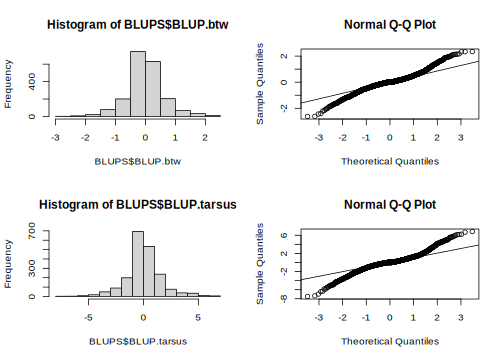
\includegraphics{wam_tuto_files/figure-latex/unnamed-chunk-107-1.pdf}

Here, some simple codes to plot the genetic correlation.

\begin{Shaded}
\begin{Highlighting}[]
\NormalTok{FEM \textless{}{-}}\StringTok{ }\KeywordTok{subset}\NormalTok{(BLUPS, SEX }\OperatorTok{==}\StringTok{ "1"}\NormalTok{)}
\NormalTok{MAL \textless{}{-}}\StringTok{ }\KeywordTok{subset}\NormalTok{(BLUPS, SEX }\OperatorTok{==}\StringTok{ "2"}\NormalTok{)}
\CommentTok{\#}
\KeywordTok{par}\NormalTok{(}\DataTypeTok{mfrow =} \KeywordTok{c}\NormalTok{(}\DecValTok{1}\NormalTok{, }\DecValTok{2}\NormalTok{))}
\CommentTok{\#}
\KeywordTok{plot}\NormalTok{(BLUP.tarsus }\OperatorTok{\textasciitilde{}}\StringTok{ }\NormalTok{BLUP.btw, FEM, }\DataTypeTok{xlab =} \StringTok{""}\NormalTok{, }\DataTypeTok{ylab =} \StringTok{""}\NormalTok{, }\DataTypeTok{las =} \FloatTok{1.2}\NormalTok{, }\DataTypeTok{bty =} \StringTok{"o"}\NormalTok{, }\DataTypeTok{col =} \StringTok{"white"}\NormalTok{)}
\KeywordTok{arrows}\NormalTok{(}\DataTypeTok{x0 =}\NormalTok{ FEM}\OperatorTok{$}\NormalTok{BLUP.btw, }\DataTypeTok{y0 =}\NormalTok{ FEM}\OperatorTok{$}\NormalTok{BLUP.tarsus }\OperatorTok{{-}}\StringTok{ }\NormalTok{FEM}\OperatorTok{$}\NormalTok{SE.tarsus, }\DataTypeTok{x1 =}\NormalTok{ FEM}\OperatorTok{$}\NormalTok{BLUP.btw, }\DataTypeTok{y1 =}\NormalTok{ FEM}\OperatorTok{$}\NormalTok{BLUP.tarsus }\OperatorTok{+}\StringTok{ }\NormalTok{FEM}\OperatorTok{$}\NormalTok{SE.tarsus, }\DataTypeTok{col =} \StringTok{"black"}\NormalTok{, }\DataTypeTok{code =} \DecValTok{3}\NormalTok{, }\DataTypeTok{angle =} \DecValTok{90}\NormalTok{, }\DataTypeTok{length =} \DecValTok{0}\NormalTok{)}
\KeywordTok{arrows}\NormalTok{(}\DataTypeTok{x0 =}\NormalTok{ FEM}\OperatorTok{$}\NormalTok{BLUP.btw }\OperatorTok{{-}}\StringTok{ }\NormalTok{FEM}\OperatorTok{$}\NormalTok{SE.btw, }\DataTypeTok{y0 =}\NormalTok{ FEM}\OperatorTok{$}\NormalTok{BLUP.tarsus, }\DataTypeTok{x1 =}\NormalTok{ FEM}\OperatorTok{$}\NormalTok{BLUP.btw }\OperatorTok{+}\StringTok{ }\NormalTok{FEM}\OperatorTok{$}\NormalTok{SE.btw, }\DataTypeTok{y1 =}\NormalTok{ FEM}\OperatorTok{$}\NormalTok{BLUP.tarsus, }\DataTypeTok{col =} \StringTok{"black"}\NormalTok{, }\DataTypeTok{code =} \DecValTok{3}\NormalTok{, }\DataTypeTok{angle =} \DecValTok{90}\NormalTok{, }\DataTypeTok{length =} \DecValTok{0}\NormalTok{)}
\KeywordTok{points}\NormalTok{(BLUP.tarsus }\OperatorTok{\textasciitilde{}}\StringTok{ }\NormalTok{BLUP.btw, FEM, }\DataTypeTok{pch =} \DecValTok{16}\NormalTok{, }\DataTypeTok{col =} \StringTok{"red"}\NormalTok{, }\DataTypeTok{cex =} \FloatTok{1.5}\NormalTok{)}
\KeywordTok{points}\NormalTok{(BLUP.tarsus }\OperatorTok{\textasciitilde{}}\StringTok{ }\NormalTok{BLUP.btw, FEM, }\DataTypeTok{pch =} \DecValTok{1}\NormalTok{, }\DataTypeTok{col =} \KeywordTok{rgb}\NormalTok{(}\DecValTok{0}\NormalTok{, }\DecValTok{0}\NormalTok{, }\DecValTok{0}\NormalTok{, }\FloatTok{0.3}\NormalTok{), }\DataTypeTok{cex =} \KeywordTok{c}\NormalTok{(}\FloatTok{1.5}\NormalTok{))}
\KeywordTok{mtext}\NormalTok{(}\StringTok{"btw (BV±SE)"}\NormalTok{, }\DataTypeTok{side =} \DecValTok{1}\NormalTok{, }\DataTypeTok{line =} \FloatTok{2.4}\NormalTok{)}
\KeywordTok{mtext}\NormalTok{(}\StringTok{"tarsus (BV±SE)"}\NormalTok{, }\DataTypeTok{side =} \DecValTok{2}\NormalTok{, }\DataTypeTok{line =} \DecValTok{2}\NormalTok{, }\DataTypeTok{las =} \DecValTok{3}\NormalTok{)}
\CommentTok{\#}
\KeywordTok{plot}\NormalTok{(BLUP.tarsus }\OperatorTok{\textasciitilde{}}\StringTok{ }\NormalTok{BLUP.btw, MAL, }\DataTypeTok{xlab =} \StringTok{""}\NormalTok{, }\DataTypeTok{ylab =} \StringTok{""}\NormalTok{, }\DataTypeTok{las =} \FloatTok{1.2}\NormalTok{, }\DataTypeTok{bty =} \StringTok{"o"}\NormalTok{, }\DataTypeTok{col =} \StringTok{"white"}\NormalTok{)}
\KeywordTok{arrows}\NormalTok{(}\DataTypeTok{x0 =}\NormalTok{ MAL}\OperatorTok{$}\NormalTok{BLUP.btw, }\DataTypeTok{y0 =}\NormalTok{ MAL}\OperatorTok{$}\NormalTok{BLUP.tarsus }\OperatorTok{{-}}\StringTok{ }\NormalTok{MAL}\OperatorTok{$}\NormalTok{SE.tarsus, }\DataTypeTok{x1 =}\NormalTok{ MAL}\OperatorTok{$}\NormalTok{BLUP.btw, }\DataTypeTok{y1 =}\NormalTok{ MAL}\OperatorTok{$}\NormalTok{BLUP.tarsus }\OperatorTok{+}\StringTok{ }\NormalTok{MAL}\OperatorTok{$}\NormalTok{SE.tarsus, }\DataTypeTok{col =} \StringTok{"black"}\NormalTok{, }\DataTypeTok{code =} \DecValTok{3}\NormalTok{, }\DataTypeTok{angle =} \DecValTok{90}\NormalTok{, }\DataTypeTok{length =} \DecValTok{0}\NormalTok{)}
\KeywordTok{arrows}\NormalTok{(}\DataTypeTok{x0 =}\NormalTok{ MAL}\OperatorTok{$}\NormalTok{BLUP.btw }\OperatorTok{{-}}\StringTok{ }\NormalTok{MAL}\OperatorTok{$}\NormalTok{SE.btw, }\DataTypeTok{y0 =}\NormalTok{ MAL}\OperatorTok{$}\NormalTok{BLUP.tarsus, }\DataTypeTok{x1 =}\NormalTok{ MAL}\OperatorTok{$}\NormalTok{BLUP.btw }\OperatorTok{+}\StringTok{ }\NormalTok{MAL}\OperatorTok{$}\NormalTok{SE.btw, }\DataTypeTok{y1 =}\NormalTok{ MAL}\OperatorTok{$}\NormalTok{BLUP.tarsus, }\DataTypeTok{col =} \StringTok{"black"}\NormalTok{, }\DataTypeTok{code =} \DecValTok{3}\NormalTok{, }\DataTypeTok{angle =} \DecValTok{90}\NormalTok{, }\DataTypeTok{length =} \DecValTok{0}\NormalTok{)}
\KeywordTok{points}\NormalTok{(BLUP.tarsus }\OperatorTok{\textasciitilde{}}\StringTok{ }\NormalTok{BLUP.btw, MAL, }\DataTypeTok{pch =} \DecValTok{16}\NormalTok{, }\DataTypeTok{col =} \StringTok{"blue"}\NormalTok{, }\DataTypeTok{cex =} \FloatTok{1.5}\NormalTok{)}
\KeywordTok{points}\NormalTok{(BLUP.tarsus }\OperatorTok{\textasciitilde{}}\StringTok{ }\NormalTok{BLUP.btw, MAL, }\DataTypeTok{pch =} \DecValTok{1}\NormalTok{, }\DataTypeTok{col =} \KeywordTok{rgb}\NormalTok{(}\DecValTok{0}\NormalTok{, }\DecValTok{0}\NormalTok{, }\DecValTok{0}\NormalTok{, }\FloatTok{0.3}\NormalTok{), }\DataTypeTok{cex =} \KeywordTok{c}\NormalTok{(}\FloatTok{1.5}\NormalTok{))}
\KeywordTok{mtext}\NormalTok{(}\StringTok{"btw (BV±SE)"}\NormalTok{, }\DataTypeTok{side =} \DecValTok{1}\NormalTok{, }\DataTypeTok{line =} \FloatTok{2.4}\NormalTok{)}
\KeywordTok{mtext}\NormalTok{(}\StringTok{"tarsus (BV±SE)"}\NormalTok{, }\DataTypeTok{side =} \DecValTok{2}\NormalTok{, }\DataTypeTok{line =} \DecValTok{2}\NormalTok{, }\DataTypeTok{las =} \DecValTok{3}\NormalTok{)}
\end{Highlighting}
\end{Shaded}

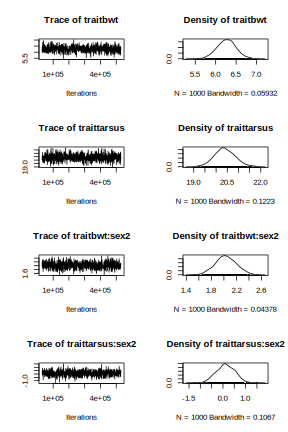
\includegraphics{wam_tuto_files/figure-latex/unnamed-chunk-108-1.pdf}

\hypertarget{between-groups-covariances-and-the-b-matrix}{%
\subsection{Between groups (co)variances and the B-matrix}\label{between-groups-covariances-and-the-b-matrix}}

Animal models are amazing model. With different group within a population, it is also possible to estimate how much the different groups shared the same genetic via the cross-group genetic covariance.
This covariance is essential to understand ontogenic or sexual conflict, which can constraint or enhanced response to evolution.
As an example, we estimate the cross-sex genetic correlation \texttt{r\_\{fm\}}

First, we need to dissociate the trait values for females and males into distinct variables. Then, we use a bivariate model (for one trait: \texttt{tarsus}) and a multivariate model (for various traits: \texttt{tarsus} and \texttt{bwt}). With a multivariate model, the cross-sex-cross trait covariance matrixis also named \texttt{B\ matrix}.

The coding is a bit complain but pretty straightforward. It is important to modify the covariance matrix at the residual level to avoid the calculation of a cross-sex residual covariance (no individual switched sex during the experiment).

\begin{Shaded}
\begin{Highlighting}[]
\NormalTok{gryphon}\OperatorTok{$}\NormalTok{bwt}\FloatTok{.1}\NormalTok{ \textless{}{-}}\StringTok{ }\OtherTok{NA}
\NormalTok{gryphon}\OperatorTok{$}\NormalTok{tarsus}\FloatTok{.1}\NormalTok{ \textless{}{-}}\StringTok{ }\OtherTok{NA}
\NormalTok{animal \textless{}{-}}\StringTok{ }\NormalTok{gryphon[gryphon}\OperatorTok{$}\NormalTok{sex }\OperatorTok{==}\StringTok{ "1"}\NormalTok{, ]}\OperatorTok{$}\NormalTok{animal}
\ControlFlowTok{for}\NormalTok{ (i }\ControlFlowTok{in} \KeywordTok{unique}\NormalTok{(animal)) \{}
\NormalTok{  gryphon}\OperatorTok{$}\NormalTok{bwt}\FloatTok{.1}\NormalTok{[}\KeywordTok{which}\NormalTok{(gryphon}\OperatorTok{$}\NormalTok{animal }\OperatorTok{==}\StringTok{ }\NormalTok{i)] \textless{}{-}}\StringTok{ }\NormalTok{gryphon}\OperatorTok{$}\NormalTok{bwt[}\KeywordTok{which}\NormalTok{(gryphon}\OperatorTok{$}\NormalTok{animal }\OperatorTok{==}\StringTok{ }\NormalTok{i)]}
\NormalTok{  gryphon}\OperatorTok{$}\NormalTok{tarsus}\FloatTok{.1}\NormalTok{[}\KeywordTok{which}\NormalTok{(gryphon}\OperatorTok{$}\NormalTok{animal }\OperatorTok{==}\StringTok{ }\NormalTok{i)] \textless{}{-}}\StringTok{ }\NormalTok{gryphon}\OperatorTok{$}\NormalTok{tarsus[}\KeywordTok{which}\NormalTok{(gryphon}\OperatorTok{$}\NormalTok{animal }\OperatorTok{==}\StringTok{ }\NormalTok{i)]}
\NormalTok{\}}
\CommentTok{\#}
\NormalTok{gryphon}\OperatorTok{$}\NormalTok{bwt}\FloatTok{.2}\NormalTok{ \textless{}{-}}\StringTok{ }\OtherTok{NA}
\NormalTok{gryphon}\OperatorTok{$}\NormalTok{tarsus}\FloatTok{.2}\NormalTok{ \textless{}{-}}\StringTok{ }\OtherTok{NA}
\NormalTok{animal \textless{}{-}}\StringTok{ }\NormalTok{gryphon[gryphon}\OperatorTok{$}\NormalTok{sex }\OperatorTok{==}\StringTok{ "2"}\NormalTok{, ]}\OperatorTok{$}\NormalTok{animal}
\ControlFlowTok{for}\NormalTok{ (i }\ControlFlowTok{in} \KeywordTok{unique}\NormalTok{(animal)) \{}
\NormalTok{  gryphon}\OperatorTok{$}\NormalTok{bwt}\FloatTok{.2}\NormalTok{[}\KeywordTok{which}\NormalTok{(gryphon}\OperatorTok{$}\NormalTok{animal }\OperatorTok{==}\StringTok{ }\NormalTok{i)] \textless{}{-}}\StringTok{ }\NormalTok{gryphon}\OperatorTok{$}\NormalTok{bwt[}\KeywordTok{which}\NormalTok{(gryphon}\OperatorTok{$}\NormalTok{animal }\OperatorTok{==}\StringTok{ }\NormalTok{i)]}
\NormalTok{  gryphon}\OperatorTok{$}\NormalTok{tarsus}\FloatTok{.2}\NormalTok{[}\KeywordTok{which}\NormalTok{(gryphon}\OperatorTok{$}\NormalTok{animal }\OperatorTok{==}\StringTok{ }\NormalTok{i)] \textless{}{-}}\StringTok{ }\NormalTok{gryphon}\OperatorTok{$}\NormalTok{tarsus[}\KeywordTok{which}\NormalTok{(gryphon}\OperatorTok{$}\NormalTok{animal }\OperatorTok{==}\StringTok{ }\NormalTok{i)]}
\NormalTok{\}}

\CommentTok{\#\#\#\#\#\#\#\#\#\#\#}
\NormalTok{temp \textless{}{-}}\StringTok{ }\KeywordTok{asreml}\NormalTok{(}\KeywordTok{cbind}\NormalTok{(tarsus}\FloatTok{.1}\NormalTok{, tarsus}\FloatTok{.2}\NormalTok{) }\OperatorTok{\textasciitilde{}}\StringTok{ }\NormalTok{trait,}
  \DataTypeTok{random =} \OperatorTok{\textasciitilde{}}\StringTok{ }\KeywordTok{us}\NormalTok{(trait)}\OperatorTok{:}\KeywordTok{vm}\NormalTok{(animal, ainv) }\OperatorTok{+}
\StringTok{    }\KeywordTok{diag}\NormalTok{(trait)}\OperatorTok{:}\NormalTok{byear }\OperatorTok{+}\StringTok{ }\KeywordTok{diag}\NormalTok{(trait)}\OperatorTok{:}\NormalTok{mother,}
  \DataTypeTok{residual =} \OperatorTok{\textasciitilde{}}\StringTok{ }\NormalTok{units}\OperatorTok{:}\KeywordTok{us}\NormalTok{(trait),}
  \DataTypeTok{data =}\NormalTok{ gryphon, }\DataTypeTok{na.action =} \KeywordTok{na.method}\NormalTok{(}\DataTypeTok{y =} \StringTok{"include"}\NormalTok{, }\DataTypeTok{x =} \StringTok{"include"}\NormalTok{), }\DataTypeTok{maxiter =} \DecValTok{20}\NormalTok{,}
  \DataTypeTok{start.values =}\NormalTok{ T}
\NormalTok{)}
\NormalTok{G \textless{}{-}}\StringTok{ }\NormalTok{temp}\OperatorTok{$}\NormalTok{vparameters[(}\DecValTok{1}\OperatorTok{:}\DecValTok{7}\NormalTok{), ]}
\NormalTok{R \textless{}{-}}\StringTok{ }\NormalTok{temp}\OperatorTok{$}\NormalTok{vparameters[}\OperatorTok{{-}}\NormalTok{(}\DecValTok{1}\OperatorTok{:}\DecValTok{7}\NormalTok{), ]}
\CommentTok{\#}
\NormalTok{G}\OperatorTok{$}\NormalTok{Constraint \textless{}{-}}\StringTok{ "U"}
\NormalTok{R}\OperatorTok{$}\NormalTok{Value[}\DecValTok{3}\NormalTok{] \textless{}{-}}\StringTok{ }\DecValTok{0}
\NormalTok{R}\OperatorTok{$}\NormalTok{Constraint[}\DecValTok{3}\NormalTok{] \textless{}{-}}\StringTok{ "F"}
\CommentTok{\#}
\NormalTok{model.BiV\_Sex \textless{}{-}}\StringTok{ }\KeywordTok{asreml}\NormalTok{(}\KeywordTok{cbind}\NormalTok{(tarsus}\FloatTok{.1}\NormalTok{, tarsus}\FloatTok{.2}\NormalTok{) }\OperatorTok{\textasciitilde{}}\StringTok{ }\NormalTok{trait,}
  \DataTypeTok{random =} \OperatorTok{\textasciitilde{}}\StringTok{ }\KeywordTok{us}\NormalTok{(trait)}\OperatorTok{:}\KeywordTok{vm}\NormalTok{(animal, ainv) }\OperatorTok{+}
\StringTok{    }\KeywordTok{diag}\NormalTok{(trait)}\OperatorTok{:}\NormalTok{byear }\OperatorTok{+}\StringTok{ }\KeywordTok{diag}\NormalTok{(trait)}\OperatorTok{:}\NormalTok{mother,}
  \DataTypeTok{residual =} \OperatorTok{\textasciitilde{}}\StringTok{ }\NormalTok{units}\OperatorTok{:}\KeywordTok{us}\NormalTok{(trait),}
  \DataTypeTok{data =}\NormalTok{ gryphon, }\DataTypeTok{na.action =} \KeywordTok{na.method}\NormalTok{(}\DataTypeTok{y =} \StringTok{"include"}\NormalTok{, }\DataTypeTok{x =} \StringTok{"include"}\NormalTok{), }\DataTypeTok{maxiter =} \DecValTok{20}\NormalTok{,}
  \DataTypeTok{G.param =}\NormalTok{ G, }\DataTypeTok{R.param =}\NormalTok{ R}
\NormalTok{)}
\end{Highlighting}
\end{Shaded}

\begin{verbatim}
## Model fitted using the sigma parameterization.
## ASReml 4.1.0 Sat Apr 30 11:10:35 2022
##           LogLik        Sigma2     DF     wall    cpu
##  1     -1494.807           1.0    681 11:10:35    0.0 (1 restrained)
##  2     -1484.793           1.0    681 11:10:35    0.0 (1 restrained)
##  3     -1475.726           1.0    681 11:10:35    0.0 (1 restrained)
##  4     -1471.905           1.0    681 11:10:35    0.0 (1 restrained)
##  5     -1470.716           1.0    681 11:10:35    0.0
##  6     -1468.154           1.0    681 11:10:35    0.0
##  7     -1467.969           1.0    681 11:10:35    0.0
##  8     -1467.967           1.0    681 11:10:35    0.0
\end{verbatim}

\begin{Shaded}
\begin{Highlighting}[]
\NormalTok{model.BiV\_Sex \textless{}{-}}\StringTok{ }\KeywordTok{update.asreml}\NormalTok{(model.BiV\_Sex)}
\end{Highlighting}
\end{Shaded}

\begin{verbatim}
## Model fitted using the sigma parameterization.
## ASReml 4.1.0 Sat Apr 30 11:10:35 2022
##           LogLik        Sigma2     DF     wall    cpu
##  1     -1467.967           1.0    681 11:10:35    0.0
##  2     -1467.967           1.0    681 11:10:35    0.0
\end{verbatim}

\begin{Shaded}
\begin{Highlighting}[]
\CommentTok{\#}
\KeywordTok{summary}\NormalTok{(model.BiV\_Sex)}\OperatorTok{$}\NormalTok{varcomp}
\end{Highlighting}
\end{Shaded}

\begin{verbatim}
##                                                component std.error   z.ratio
## trait:byear!trait_tarsus.1                      3.280319  1.532909 2.1399299
## trait:byear!trait_tarsus.2                      4.743134  1.891252 2.5079332
## trait:mother!trait_tarsus.1                     1.875132  2.424092 0.7735398
## trait:mother!trait_tarsus.2                     4.314158  2.785254 1.5489283
## trait:vm(animal, ainv)!trait_tarsus.1:tarsus.1  6.582654  3.636467 1.8101781
## trait:vm(animal, ainv)!trait_tarsus.2:tarsus.1  8.396245  3.278591 2.5609306
## trait:vm(animal, ainv)!trait_tarsus.2:tarsus.2 12.898424  8.038362 1.6046084
## units:trait!R                                   1.000000        NA        NA
## units:trait!trait_tarsus.1:tarsus.1            14.872757  3.637545 4.0886803
## units:trait!trait_tarsus.2:tarsus.1             0.000000        NA        NA
## units:trait!trait_tarsus.2:tarsus.2            10.760849  6.294585 1.7095406
##                                                bound %ch
## trait:byear!trait_tarsus.1                         U   0
## trait:byear!trait_tarsus.2                         U   0
## trait:mother!trait_tarsus.1                        U   0
## trait:mother!trait_tarsus.2                        U   0
## trait:vm(animal, ainv)!trait_tarsus.1:tarsus.1     U   0
## trait:vm(animal, ainv)!trait_tarsus.2:tarsus.1     U   0
## trait:vm(animal, ainv)!trait_tarsus.2:tarsus.2     U   0
## units:trait!R                                      F   0
## units:trait!trait_tarsus.1:tarsus.1                P   0
## units:trait!trait_tarsus.2:tarsus.1                F  NA
## units:trait!trait_tarsus.2:tarsus.2                P   0
\end{verbatim}

The cross-sex genetic correlation can estimate form the output of the model.
For tarsus length at fledging, sexes shared a lot of genetic variance which is commun for a trait with low sexual dimorphism. If the selection is antagonistic between males and females, sexes can not evolve freely form the other sexes and a sexual conflict appears.

\begin{Shaded}
\begin{Highlighting}[]
\KeywordTok{vpredict}\NormalTok{(model.BiV\_Sex, r\_fm }\OperatorTok{\textasciitilde{}}\StringTok{ }\NormalTok{V6 }\OperatorTok{/}\StringTok{ }\KeywordTok{sqrt}\NormalTok{(V5 }\OperatorTok{*}\StringTok{ }\NormalTok{V7))}
\end{Highlighting}
\end{Shaded}

\begin{verbatim}
##       Estimate        SE
## r_fm 0.9112054 0.4229764
\end{verbatim}

We can estimate directly the correlation and plot the cross-sex genetic correlation

\begin{Shaded}
\begin{Highlighting}[]
\NormalTok{temp \textless{}{-}}\StringTok{ }\KeywordTok{asreml}\NormalTok{(}\KeywordTok{cbind}\NormalTok{(tarsus}\FloatTok{.1}\NormalTok{, tarsus}\FloatTok{.2}\NormalTok{) }\OperatorTok{\textasciitilde{}}\StringTok{ }\NormalTok{trait,}
  \DataTypeTok{random =} \OperatorTok{\textasciitilde{}}\StringTok{ }\KeywordTok{corgh}\NormalTok{(trait)}\OperatorTok{:}\KeywordTok{vm}\NormalTok{(animal, ainv) }\OperatorTok{+}
\StringTok{    }\KeywordTok{diag}\NormalTok{(trait)}\OperatorTok{:}\NormalTok{byear }\OperatorTok{+}\StringTok{ }\KeywordTok{diag}\NormalTok{(trait)}\OperatorTok{:}\NormalTok{mother,}
  \DataTypeTok{residual =} \OperatorTok{\textasciitilde{}}\StringTok{ }\NormalTok{units}\OperatorTok{:}\KeywordTok{corgh}\NormalTok{(trait),}
  \DataTypeTok{data =}\NormalTok{ gryphon, }\DataTypeTok{na.action =} \KeywordTok{na.method}\NormalTok{(}\DataTypeTok{y =} \StringTok{"include"}\NormalTok{, }\DataTypeTok{x =} \StringTok{"include"}\NormalTok{), }\DataTypeTok{maxiter =} \DecValTok{20}\NormalTok{,}
  \DataTypeTok{start.values =}\NormalTok{ T}
\NormalTok{)}
\NormalTok{G \textless{}{-}}\StringTok{ }\NormalTok{temp}\OperatorTok{$}\NormalTok{vparameters[(}\DecValTok{1}\OperatorTok{:}\DecValTok{7}\NormalTok{), ]}
\NormalTok{R \textless{}{-}}\StringTok{ }\NormalTok{temp}\OperatorTok{$}\NormalTok{vparameters[}\OperatorTok{{-}}\NormalTok{(}\DecValTok{1}\OperatorTok{:}\DecValTok{7}\NormalTok{), ]}
\CommentTok{\#}
\NormalTok{G}\OperatorTok{$}\NormalTok{Constraint \textless{}{-}}\StringTok{ "U"}
\NormalTok{R}\OperatorTok{$}\NormalTok{Value[}\DecValTok{2}\NormalTok{] \textless{}{-}}\StringTok{ }\DecValTok{0}
\NormalTok{R}\OperatorTok{$}\NormalTok{Constraint[}\DecValTok{2}\NormalTok{] \textless{}{-}}\StringTok{ "F"}
\CommentTok{\#}
\NormalTok{model.BiV\_Sex \textless{}{-}}\StringTok{ }\KeywordTok{asreml}\NormalTok{(}\KeywordTok{cbind}\NormalTok{(tarsus}\FloatTok{.1}\NormalTok{, tarsus}\FloatTok{.2}\NormalTok{) }\OperatorTok{\textasciitilde{}}\StringTok{ }\NormalTok{trait,}
  \DataTypeTok{random =} \OperatorTok{\textasciitilde{}}\StringTok{ }\KeywordTok{corgh}\NormalTok{(trait)}\OperatorTok{:}\KeywordTok{vm}\NormalTok{(animal, ainv) }\OperatorTok{+}
\StringTok{    }\KeywordTok{diag}\NormalTok{(trait)}\OperatorTok{:}\NormalTok{byear }\OperatorTok{+}\StringTok{ }\KeywordTok{diag}\NormalTok{(trait)}\OperatorTok{:}\NormalTok{mother,}
  \DataTypeTok{residual =} \OperatorTok{\textasciitilde{}}\StringTok{ }\NormalTok{units}\OperatorTok{:}\KeywordTok{corgh}\NormalTok{(trait),}
  \DataTypeTok{data =}\NormalTok{ gryphon, }\DataTypeTok{na.action =} \KeywordTok{na.method}\NormalTok{(}\DataTypeTok{y =} \StringTok{"include"}\NormalTok{, }\DataTypeTok{x =} \StringTok{"include"}\NormalTok{), }\DataTypeTok{maxiter =} \DecValTok{20}\NormalTok{,}
  \DataTypeTok{G.param =}\NormalTok{ G, }\DataTypeTok{R.param =}\NormalTok{ R}
\NormalTok{)}
\end{Highlighting}
\end{Shaded}

\begin{verbatim}
## Model fitted using the sigma parameterization.
## ASReml 4.1.0 Sat Apr 30 11:10:36 2022
##           LogLik        Sigma2     DF     wall    cpu
##  1     -1494.323           1.0    681 11:10:36    0.0 (1 restrained)
##  2     -1482.996           1.0    681 11:10:36    0.0 (1 restrained)
##  3     -1472.827           1.0    681 11:10:36    0.0 (1 restrained)
##  4     -1468.707           1.0    681 11:10:36    0.0
##  5     -1467.984           1.0    681 11:10:36    0.0
##  6     -1467.968           1.0    681 11:10:36    0.0
##  7     -1467.967           1.0    681 11:10:36    0.0
\end{verbatim}

\begin{Shaded}
\begin{Highlighting}[]
\NormalTok{model.BiV\_Sex \textless{}{-}}\StringTok{ }\KeywordTok{update.asreml}\NormalTok{(model.BiV\_Sex)}
\end{Highlighting}
\end{Shaded}

\begin{verbatim}
## Model fitted using the sigma parameterization.
## ASReml 4.1.0 Sat Apr 30 11:10:36 2022
##           LogLik        Sigma2     DF     wall    cpu
##  1     -1467.967           1.0    681 11:10:36    0.0
##  2     -1467.967           1.0    681 11:10:36    0.0
\end{verbatim}

\begin{Shaded}
\begin{Highlighting}[]
\CommentTok{\#}
\KeywordTok{summary}\NormalTok{(model.BiV\_Sex)}\OperatorTok{$}\NormalTok{varcomp}
\end{Highlighting}
\end{Shaded}

\begin{verbatim}
##                                                            component std.error
## trait:byear!trait_tarsus.1                                 3.2803263 1.5329224
## trait:byear!trait_tarsus.2                                 4.7431679 1.8913244
## trait:mother!trait_tarsus.1                                1.8751274 2.4240942
## trait:mother!trait_tarsus.2                                4.3141262 2.7852550
## trait:vm(animal, ainv)!trait!tarsus.2:!trait!tarsus.1.cor  0.9111864 0.4230261
## trait:vm(animal, ainv)!trait_tarsus.1                      6.5826478 3.6364929
## trait:vm(animal, ainv)!trait_tarsus.2                     12.8988848 8.0388517
## units:trait!R                                              1.0000000        NA
## units:trait!trait!tarsus.2:!trait!tarsus.1.cor             0.0000000        NA
## units:trait!trait_tarsus.1                                14.8727602 3.6375549
## units:trait!trait_tarsus.2                                10.7604420 6.2948051
##                                                             z.ratio bound %ch
## trait:byear!trait_tarsus.1                                2.1399167     U   0
## trait:byear!trait_tarsus.2                                2.5078553     U   0
## trait:mother!trait_tarsus.1                               0.7735373     U   0
## trait:mother!trait_tarsus.2                               1.5489160     U   0
## trait:vm(animal, ainv)!trait!tarsus.2:!trait!tarsus.1.cor 2.1539720     U   0
## trait:vm(animal, ainv)!trait_tarsus.1                     1.8101638     U   0
## trait:vm(animal, ainv)!trait_tarsus.2                     1.6045681     U   0
## units:trait!R                                                    NA     F   0
## units:trait!trait!tarsus.2:!trait!tarsus.1.cor                   NA     F  NA
## units:trait!trait_tarsus.1                                4.0886696     P   0
## units:trait!trait_tarsus.2                                1.7094162     P   0
\end{verbatim}

\begin{Shaded}
\begin{Highlighting}[]
\CommentTok{\#\#\#\#\#\#\#\#\#\#\#}
\NormalTok{DvsS \textless{}{-}}\StringTok{ }\KeywordTok{data.frame}\NormalTok{(}
  \DataTypeTok{Trait =} \KeywordTok{rownames}\NormalTok{(model.BiV\_Sex}\OperatorTok{$}\NormalTok{coefficients}\OperatorTok{$}\NormalTok{random),}
  \DataTypeTok{BLUP =}\NormalTok{ model.BiV\_Sex}\OperatorTok{$}\NormalTok{coefficients}\OperatorTok{$}\NormalTok{random,}
  \DataTypeTok{SE =} \KeywordTok{sqrt}\NormalTok{(model.BiV\_Sex}\OperatorTok{$}\NormalTok{vcoeff}\OperatorTok{$}\NormalTok{random }\OperatorTok{*}\StringTok{ }\NormalTok{model.BiV\_Sex}\OperatorTok{$}\NormalTok{sigma2)}
\NormalTok{)}
\NormalTok{DvsS}\OperatorTok{$}\NormalTok{ID \textless{}{-}}\StringTok{ }\KeywordTok{substr}\NormalTok{(DvsS}\OperatorTok{$}\NormalTok{Trait, }\DecValTok{33}\NormalTok{, }\DecValTok{35}\NormalTok{)}
\NormalTok{DvsS}\OperatorTok{$}\NormalTok{TRAIT \textless{}{-}}\StringTok{ }\KeywordTok{substr}\NormalTok{(DvsS}\OperatorTok{$}\NormalTok{Trait, }\DecValTok{7}\NormalTok{, }\DecValTok{14}\NormalTok{)}
\NormalTok{DvsS \textless{}{-}}\StringTok{ }\NormalTok{DvsS[}\DecValTok{927}\OperatorTok{:}\DecValTok{3544}\NormalTok{, ] }\CommentTok{\# keep only row associated to animal}
\KeywordTok{summary}\NormalTok{(}\KeywordTok{factor}\NormalTok{(DvsS}\OperatorTok{$}\NormalTok{TRAIT))}
\end{Highlighting}
\end{Shaded}

\begin{verbatim}
## tarsus.1 tarsus.2 
##     1309     1309
\end{verbatim}

\begin{Shaded}
\begin{Highlighting}[]
\CommentTok{\#}
\NormalTok{DvsS}\OperatorTok{$}\NormalTok{Trait \textless{}{-}}\StringTok{ }\OtherTok{NULL}
\KeywordTok{colnames}\NormalTok{(DvsS)[}\DecValTok{1}\NormalTok{] \textless{}{-}}\StringTok{ "BLUP"}
\NormalTok{BLUPS \textless{}{-}}\StringTok{ }\KeywordTok{reshape}\NormalTok{(DvsS, }\DataTypeTok{v.names =} \KeywordTok{c}\NormalTok{(}\StringTok{"BLUP"}\NormalTok{, }\StringTok{"SE"}\NormalTok{), }\DataTypeTok{idvar =} \StringTok{"ID"}\NormalTok{, }\DataTypeTok{timevar =} \StringTok{"TRAIT"}\NormalTok{, }\DataTypeTok{direction =} \StringTok{"wide"}\NormalTok{)}
\end{Highlighting}
\end{Shaded}

\begin{verbatim}
## Warning in reshapeWide(data, idvar = idvar, timevar = timevar, varying =
## varying, : multiple rows match for TRAIT=tarsus.1: first taken
\end{verbatim}

\begin{verbatim}
## Warning in reshapeWide(data, idvar = idvar, timevar = timevar, varying =
## varying, : multiple rows match for TRAIT=tarsus.2: first taken
\end{verbatim}

\begin{Shaded}
\begin{Highlighting}[]
\KeywordTok{nrow}\NormalTok{(BLUPS)}
\end{Highlighting}
\end{Shaded}

\begin{verbatim}
## [1] 999
\end{verbatim}

\begin{Shaded}
\begin{Highlighting}[]
\KeywordTok{rownames}\NormalTok{(BLUPS) \textless{}{-}}\StringTok{ }\KeywordTok{c}\NormalTok{()}
\KeywordTok{colnames}\NormalTok{(BLUPS) \textless{}{-}}\StringTok{ }\KeywordTok{c}\NormalTok{(}\StringTok{"ID"}\NormalTok{, }\StringTok{"BLUP.1"}\NormalTok{, }\StringTok{"SE.1"}\NormalTok{, }\StringTok{"BLUP.2"}\NormalTok{, }\StringTok{"SE.2"}\NormalTok{)}
\KeywordTok{summary}\NormalTok{(BLUPS)}
\end{Highlighting}
\end{Shaded}

\begin{verbatim}
##       ID                BLUP.1              SE.1           BLUP.2        
##  Length:999         Min.   :-4.27022   Min.   :1.724   Min.   :-5.98516  
##  Class :character   1st Qu.:-0.69816   1st Qu.:2.010   1st Qu.:-0.99808  
##  Mode  :character   Median : 0.00000   Median :2.143   Median : 0.00000  
##                     Mean   : 0.05588   Mean   :2.204   Mean   : 0.06904  
##                     3rd Qu.: 0.84250   3rd Qu.:2.426   3rd Qu.: 1.13426  
##                     Max.   : 4.55405   Max.   :2.567   Max.   : 6.35309  
##       SE.2      
##  Min.   :2.375  
##  1st Qu.:2.677  
##  Median :3.055  
##  Mean   :3.047  
##  3rd Qu.:3.378  
##  Max.   :3.591
\end{verbatim}

\begin{Shaded}
\begin{Highlighting}[]
\CommentTok{\#\#\#\#\#\#\#\#\#\#\#}
\NormalTok{Y \textless{}{-}}\StringTok{ }\NormalTok{BLUPS}\OperatorTok{$}\NormalTok{BLUP}\FloatTok{.1}
\NormalTok{X \textless{}{-}}\StringTok{ }\NormalTok{BLUPS}\OperatorTok{$}\NormalTok{BLUP}\FloatTok{.2}
\NormalTok{se.Y \textless{}{-}}\StringTok{ }\NormalTok{BLUPS}\OperatorTok{$}\NormalTok{SE}\FloatTok{.1}
\NormalTok{se.X \textless{}{-}}\StringTok{ }\NormalTok{BLUPS}\OperatorTok{$}\NormalTok{SE}\FloatTok{.2}

\KeywordTok{plot}\NormalTok{(X, Y, }\DataTypeTok{xlab =} \StringTok{""}\NormalTok{, }\DataTypeTok{ylab =} \StringTok{""}\NormalTok{, }\DataTypeTok{las =} \FloatTok{1.2}\NormalTok{, }\DataTypeTok{bty =} \StringTok{"o"}\NormalTok{, }\DataTypeTok{col =} \StringTok{"white"}\NormalTok{)}
\KeywordTok{arrows}\NormalTok{(}\DataTypeTok{x0 =}\NormalTok{ X, }\DataTypeTok{y0 =}\NormalTok{ Y }\OperatorTok{{-}}\StringTok{ }\NormalTok{se.Y, }\DataTypeTok{x1 =}\NormalTok{ X, }\DataTypeTok{y1 =}\NormalTok{ Y }\OperatorTok{+}\StringTok{ }\NormalTok{se.Y, }\DataTypeTok{col =} \KeywordTok{rgb}\NormalTok{(}\DecValTok{0}\NormalTok{, }\DecValTok{0}\NormalTok{, }\DecValTok{0}\NormalTok{, }\FloatTok{0.2}\NormalTok{), }\DataTypeTok{code =} \DecValTok{3}\NormalTok{, }\DataTypeTok{angle =} \DecValTok{90}\NormalTok{, }\DataTypeTok{length =} \DecValTok{0}\NormalTok{)}
\KeywordTok{arrows}\NormalTok{(}\DataTypeTok{x0 =}\NormalTok{ X }\OperatorTok{{-}}\StringTok{ }\NormalTok{se.X, }\DataTypeTok{y0 =}\NormalTok{ Y, }\DataTypeTok{x1 =}\NormalTok{ X }\OperatorTok{+}\StringTok{ }\NormalTok{se.X, }\DataTypeTok{y1 =}\NormalTok{ Y, }\DataTypeTok{col =} \KeywordTok{rgb}\NormalTok{(}\DecValTok{0}\NormalTok{, }\DecValTok{0}\NormalTok{, }\DecValTok{0}\NormalTok{, }\FloatTok{0.2}\NormalTok{), }\DataTypeTok{code =} \DecValTok{3}\NormalTok{, }\DataTypeTok{angle =} \DecValTok{90}\NormalTok{, }\DataTypeTok{length =} \DecValTok{0}\NormalTok{)}
\KeywordTok{points}\NormalTok{(X, Y, }\DataTypeTok{pch =} \DecValTok{1}\NormalTok{, }\DataTypeTok{col =} \KeywordTok{rgb}\NormalTok{(}\DecValTok{1}\NormalTok{, }\DecValTok{0}\NormalTok{, }\DecValTok{1}\NormalTok{, }\FloatTok{0.2}\NormalTok{), }\DataTypeTok{cex =} \FloatTok{1.5}\NormalTok{)}
\KeywordTok{points}\NormalTok{(X, Y, }\DataTypeTok{pch =} \DecValTok{16}\NormalTok{, }\DataTypeTok{col =} \KeywordTok{rgb}\NormalTok{(}\DecValTok{1}\NormalTok{, }\DecValTok{0}\NormalTok{, }\DecValTok{1}\NormalTok{, }\FloatTok{0.2}\NormalTok{), }\DataTypeTok{cex =} \FloatTok{1.5}\NormalTok{)}
\CommentTok{\# abline(v=0,lty=3);abline(h=0,lty=3)}
\KeywordTok{mtext}\NormalTok{(}\StringTok{"Male tarsus (BV±SE)"}\NormalTok{, }\DataTypeTok{side =} \DecValTok{2}\NormalTok{, }\DataTypeTok{line =} \DecValTok{2}\NormalTok{, }\DataTypeTok{las =} \DecValTok{3}\NormalTok{)}
\KeywordTok{mtext}\NormalTok{(}\StringTok{"Female tarsus (BV±SE)"}\NormalTok{, }\DataTypeTok{side =} \DecValTok{1}\NormalTok{, }\DataTypeTok{line =} \FloatTok{2.2}\NormalTok{)}
\end{Highlighting}
\end{Shaded}

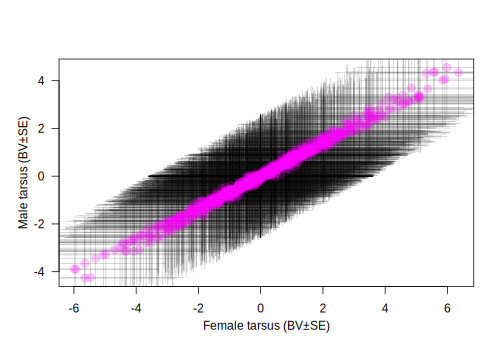
\includegraphics{wam_tuto_files/figure-latex/unnamed-chunk-111-1.pdf}

The B matrix used the same code but in a multivariate animal model framework. Here some example code, however due to the nature of the dataset, the cross-sex genetic covariance for birth weight is hard to estimate making difficulty to fit this multivariate animal model.

\begin{Shaded}
\begin{Highlighting}[]
\NormalTok{temp \textless{}{-}}\StringTok{ }\KeywordTok{asreml}\NormalTok{(}\KeywordTok{cbind}\NormalTok{(tarsus}\FloatTok{.1}\NormalTok{, bwt}\FloatTok{.1}\NormalTok{, tarsus}\FloatTok{.2}\NormalTok{, bwt}\FloatTok{.2}\NormalTok{) }\OperatorTok{\textasciitilde{}}\StringTok{ }\NormalTok{trait,}
  \DataTypeTok{random =} \OperatorTok{\textasciitilde{}}\StringTok{ }\KeywordTok{us}\NormalTok{(trait)}\OperatorTok{:}\KeywordTok{vm}\NormalTok{(animal, ainv) }\OperatorTok{+}
\StringTok{    }\KeywordTok{diag}\NormalTok{(trait)}\OperatorTok{:}\NormalTok{byear }\OperatorTok{+}\StringTok{ }\KeywordTok{diag}\NormalTok{(trait)}\OperatorTok{:}\NormalTok{mother,}
  \DataTypeTok{residual =} \OperatorTok{\textasciitilde{}}\StringTok{ }\NormalTok{units}\OperatorTok{:}\KeywordTok{us}\NormalTok{(trait),}
  \DataTypeTok{data =}\NormalTok{ gryphon, }\DataTypeTok{na.action =} \KeywordTok{na.method}\NormalTok{(}\DataTypeTok{y =} \StringTok{"include"}\NormalTok{, }\DataTypeTok{x =} \StringTok{"include"}\NormalTok{), }\DataTypeTok{maxiter =} \DecValTok{20}\NormalTok{,}
  \DataTypeTok{start.values =}\NormalTok{ T}
\NormalTok{)}
\NormalTok{G \textless{}{-}}\StringTok{ }\NormalTok{temp}\OperatorTok{$}\NormalTok{vparameters[(}\DecValTok{1}\OperatorTok{:}\DecValTok{18}\NormalTok{), ]}
\NormalTok{R \textless{}{-}}\StringTok{ }\NormalTok{temp}\OperatorTok{$}\NormalTok{vparameters[}\OperatorTok{{-}}\NormalTok{(}\DecValTok{1}\OperatorTok{:}\DecValTok{18}\NormalTok{), ]}
\CommentTok{\#}
\NormalTok{G}\OperatorTok{$}\NormalTok{Constraint \textless{}{-}}\StringTok{ "U"}
\NormalTok{R}\OperatorTok{$}\NormalTok{Value[}\DecValTok{5}\OperatorTok{:}\DecValTok{6}\NormalTok{] \textless{}{-}}\StringTok{ }\DecValTok{0}
\NormalTok{R}\OperatorTok{$}\NormalTok{Constraint[}\DecValTok{5}\OperatorTok{:}\DecValTok{6}\NormalTok{] \textless{}{-}}\StringTok{ "F"}
\NormalTok{R}\OperatorTok{$}\NormalTok{Value[}\DecValTok{8}\OperatorTok{:}\DecValTok{9}\NormalTok{] \textless{}{-}}\StringTok{ }\DecValTok{0}
\NormalTok{R}\OperatorTok{$}\NormalTok{Constraint[}\DecValTok{8}\OperatorTok{:}\DecValTok{9}\NormalTok{] \textless{}{-}}\StringTok{ "F"}
\CommentTok{\#}
\CommentTok{\# model.MultV\_Sex\textless{}{-}asreml(cbind(tarsus.1,bwt.1,tarsus.2,bwt.2)\textasciitilde{}trait,}
\CommentTok{\#          random=\textasciitilde{}us(trait):vm(animal,ainv)+}
\CommentTok{\#         diag(trait):byear +   diag(trait):mother,}
\CommentTok{\#         residual = \textasciitilde{}units:us(trait),}
\CommentTok{\#         data=gryphon,na.action=na.method(y="include",x="include"),maxiter=20,}
\CommentTok{\#     G.param=G,R.param=R)}
\CommentTok{\# model.MultV\_Sex\textless{}{-}update.asreml(model.MultV\_Sex)}
\CommentTok{\#}
\CommentTok{\# summary(model.MultV\_Sex)$varcomp}
\end{Highlighting}
\end{Shaded}

\hypertarget{gremlin-2}{%
\section{gremlin}\label{gremlin-2}}

Might not available yet
Meanwhile

\begin{figure}

\includegraphics[width=1\linewidth]{images/Gizmo} \caption{Keep it dry and do no feed after midnight.}\label{fig:unnamed-chunk-113}
\end{figure}

\hypertarget{mcmcglmm-2}{%
\section{MCMCglmm}\label{mcmcglmm-2}}

\texttt{MCMCglmm} has the advantage to keep automatically keep the lines with missing data and will try to fit the model use latent variables for missing data.
We will remove the missing values from the data before fitting the model.

\begin{Shaded}
\begin{Highlighting}[]
\NormalTok{gryphon2 \textless{}{-}}\StringTok{ }\KeywordTok{subset}\NormalTok{(gryphon, }\OperatorTok{!}\KeywordTok{is.na}\NormalTok{(bwt) }\OperatorTok{\&}\StringTok{ }\OperatorTok{!}\KeywordTok{is.na}\NormalTok{(tarsus))}
\end{Highlighting}
\end{Shaded}

First load MCMCglmm:

\begin{Shaded}
\begin{Highlighting}[]
\KeywordTok{library}\NormalTok{(MCMCglmm)}
\NormalTok{Ainv \textless{}{-}}\StringTok{ }\KeywordTok{inverseA}\NormalTok{(gryphonped)}\OperatorTok{$}\NormalTok{Ainv}
\end{Highlighting}
\end{Shaded}

\hypertarget{fitting-the-model}{%
\subsection{Fitting the model}\label{fitting-the-model}}

Fitting a multivariate model in MCMCglmm involves several new consideration above those for fitting univariate models. First, we have to fit multivariate priors; second, we have to specify the ways in which effects on different traits may covary, including the nature of residual (co)variation; and third, we will have to be a little more specific when specifying to MCMCglmm what type of distributions from which we assume our data are drawn. Our most basic model can be specified as:

\begin{Shaded}
\begin{Highlighting}[]
\NormalTok{prior2}\FloatTok{.1}\NormalTok{ \textless{}{-}}\StringTok{ }\KeywordTok{list}\NormalTok{(}
  \DataTypeTok{G =} \KeywordTok{list}\NormalTok{(}\DataTypeTok{G1 =} \KeywordTok{list}\NormalTok{(}\DataTypeTok{V =} \KeywordTok{diag}\NormalTok{(}\DecValTok{2}\NormalTok{), }\DataTypeTok{nu =} \FloatTok{1.002}\NormalTok{)),}
  \DataTypeTok{R =} \KeywordTok{list}\NormalTok{(}\DataTypeTok{V =} \KeywordTok{diag}\NormalTok{(}\DecValTok{2}\NormalTok{), }\DataTypeTok{nu =} \FloatTok{1.002}\NormalTok{)}
\NormalTok{)}

\NormalTok{model2}\FloatTok{.1}\NormalTok{ \textless{}{-}}\StringTok{ }\KeywordTok{MCMCglmm}\NormalTok{(}\KeywordTok{cbind}\NormalTok{(bwt, tarsus) }\OperatorTok{\textasciitilde{}}\StringTok{ }\NormalTok{trait }\OperatorTok{{-}}\StringTok{ }\DecValTok{1}\NormalTok{,}
  \DataTypeTok{random =} \OperatorTok{\textasciitilde{}}\StringTok{ }\KeywordTok{us}\NormalTok{(trait)}\OperatorTok{:}\NormalTok{animal,}
  \DataTypeTok{rcov =} \OperatorTok{\textasciitilde{}}\StringTok{ }\KeywordTok{us}\NormalTok{(trait)}\OperatorTok{:}\NormalTok{units,}
  \DataTypeTok{family =} \KeywordTok{c}\NormalTok{(}\StringTok{"gaussian"}\NormalTok{, }\StringTok{"gaussian"}\NormalTok{),}
  \DataTypeTok{ginv =} \KeywordTok{list}\NormalTok{(}\DataTypeTok{animal =}\NormalTok{ Ainv),}
  \DataTypeTok{data =}\NormalTok{ gryphon2, }\DataTypeTok{prior =}\NormalTok{ prior2}\FloatTok{.1}\NormalTok{, }\DataTypeTok{verbose =} \OtherTok{FALSE}
\NormalTok{)}
\KeywordTok{summary}\NormalTok{(model2}\FloatTok{.1}\NormalTok{)}
\end{Highlighting}
\end{Shaded}

\begin{verbatim}
## 
##  Iterations = 3001:12991
##  Thinning interval  = 10
##  Sample size  = 1000 
## 
##  DIC: 7156.888 
## 
##  G-structure:  ~us(trait):animal
## 
##                                post.mean l-95% CI u-95% CI eff.samp
## traitbwt:traitbwt.animal           3.236  1.98774    4.656   117.84
## traittarsus:traitbwt.animal        2.045 -0.02795    4.612    97.11
## traitbwt:traittarsus.animal        2.045 -0.02795    4.612    97.11
## traittarsus:traittarsus.animal    11.357  5.21354   17.365    65.68
## 
##  R-structure:  ~us(trait):units
## 
##                               post.mean l-95% CI u-95% CI eff.samp
## traitbwt:traitbwt.units           3.951    2.790    5.074    154.3
## traittarsus:traitbwt.units        3.641    1.736    5.841    115.4
## traitbwt:traittarsus.units        3.641    1.736    5.841    115.4
## traittarsus:traittarsus.units    18.646   13.084   24.144    102.7
## 
##  Location effects: cbind(bwt, tarsus) ~ trait - 1 
## 
##             post.mean l-95% CI u-95% CI eff.samp  pMCMC    
## traitbwt        7.483    7.166    7.749    609.9 <0.001 ***
## traittarsus    20.424   19.784   20.972   1000.0 <0.001 ***
## ---
## Signif. codes:  0 '***' 0.001 '**' 0.01 '*' 0.05 '.' 0.1 ' ' 1
\end{verbatim}

\begin{Shaded}
\begin{Highlighting}[]
\KeywordTok{plot}\NormalTok{(model2}\FloatTok{.1}\OperatorTok{$}\NormalTok{VCV[, }\StringTok{"traittarsus:traittarsus.animal"}\NormalTok{])}
\end{Highlighting}
\end{Shaded}

\begin{figure}
\centering
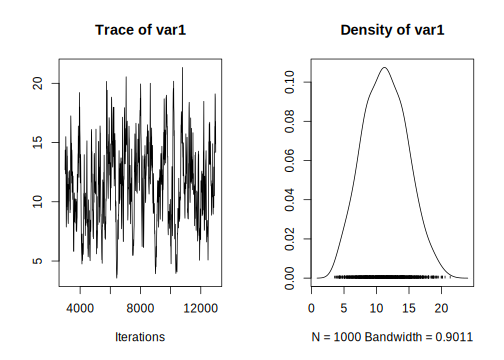
\includegraphics{wam_tuto_files/figure-latex/unnamed-chunk-116-1.pdf}
\caption{\label{fig:unnamed-chunk-116}The posterior distribution of the additive genetic effect for tarsus length in a MCMCglmm run with default values}
\end{figure}

\begin{Shaded}
\begin{Highlighting}[]
\KeywordTok{autocorr.diag}\NormalTok{(model2}\FloatTok{.1}\OperatorTok{$}\NormalTok{VCV)[, }\StringTok{"traittarsus:traittarsus.animal"}\NormalTok{][}\DecValTok{2}\NormalTok{]}
\end{Highlighting}
\end{Shaded}

\begin{verbatim}
##    Lag 10 
## 0.8199896
\end{verbatim}

We have constructed the prior similarly to the those in the univariate models in tutorial 1, only we are specifying a 2x2 covariance matrix rather than a single variance. In order to provide proper priors, we have set the degree of belief parameter to greater than 1 (1.002). Those priors are not necessarily weak or uninformative in all circumstances. We will consider them adequate nonetheless for this tutorial. Please the vignette of the MCMCglmm packages \citep{R-MCMCglmm} for more information on priors. In tutorial 1, we used full autocorrelation tables to evaluate the validity of the posterior distribution. Note that we have not done this here.

For a bivariate model this table can become very complex. Nonetheless, it is worth evaluating, rather it is simply to large to include here. It can be viewed in the console as before. Here we have displayed only the autocorrelation for estimates of additive genetic effects for tarsus length with a lag of one samples (10 iterations given this MCMCglmm run with default values). This lag of 0.8199896 is clearly unacceptable. The posterior distribution of the additive genetic effect on tarsus length is shown in Figure 4, note the autocorrelation evident in the left-hand plot.

We will opt to run the analysis for longer. This longer run could be run using the following code (including a line to save the output):

\begin{Shaded}
\begin{Highlighting}[]
\NormalTok{model2}\FloatTok{.1}\NormalTok{ \textless{}{-}}\StringTok{ }\KeywordTok{MCMCglmm}\NormalTok{(}\KeywordTok{cbind}\NormalTok{(bwt, tarsus) }\OperatorTok{\textasciitilde{}}\StringTok{ }\NormalTok{trait }\OperatorTok{{-}}\StringTok{ }\DecValTok{1}\NormalTok{,}
  \DataTypeTok{random =} \OperatorTok{\textasciitilde{}}\StringTok{ }\KeywordTok{us}\NormalTok{(trait)}\OperatorTok{:}\NormalTok{animal,}
  \DataTypeTok{rcov =} \OperatorTok{\textasciitilde{}}\StringTok{ }\KeywordTok{us}\NormalTok{(trait)}\OperatorTok{:}\NormalTok{units,}
  \DataTypeTok{family =} \KeywordTok{c}\NormalTok{(}\StringTok{"gaussian"}\NormalTok{, }\StringTok{"gaussian"}\NormalTok{),}
  \DataTypeTok{ginv =} \KeywordTok{list}\NormalTok{(}\DataTypeTok{animal =}\NormalTok{ Ainv),}
  \DataTypeTok{data =}\NormalTok{ gryphon2,}
  \DataTypeTok{nitt =} \DecValTok{130000}\NormalTok{, }\DataTypeTok{thin =} \DecValTok{100}\NormalTok{, }\DataTypeTok{burnin =} \DecValTok{30000}\NormalTok{,}
  \DataTypeTok{prior =}\NormalTok{ prior2}\FloatTok{.1}\NormalTok{, }\DataTypeTok{verbose =} \OtherTok{FALSE}
\NormalTok{)}
\KeywordTok{save}\NormalTok{(model2}\FloatTok{.1}\NormalTok{, }\DataTypeTok{file =} \StringTok{"data/MCMCglmm\_model2\_1\_LongRun.rda"}\NormalTok{)}
\end{Highlighting}
\end{Shaded}

However, this run might take as long as an hour. For the purpose of this tutorial we have provided an output for such a run. It can be obtained and manipulated as follows, assuming that the file \texttt{MCMCglmm\_model2\_1\_LongRun.rda} is available at the specified location:

\begin{Shaded}
\begin{Highlighting}[]
\KeywordTok{load}\NormalTok{(}\DataTypeTok{file =} \StringTok{"data/MCMCglmm\_model2\_1\_LongRun.rda"}\NormalTok{)}
\KeywordTok{autocorr.diag}\NormalTok{(model2}\FloatTok{.1}\OperatorTok{$}\NormalTok{VCV)[, }\StringTok{"traittarsus:traittarsus.animal"}\NormalTok{][}\DecValTok{2}\NormalTok{]}
\end{Highlighting}
\end{Shaded}

\begin{verbatim}
##   Lag 100 
## 0.2805747
\end{verbatim}

This level of autocorrelation is more acceptable, at least for the purpose of demonstration in this tutorial.
We can recover variance components, heritabilities, and genetic correlations from the posterior distribution of this model:

\begin{Shaded}
\begin{Highlighting}[]
\KeywordTok{posterior.mode}\NormalTok{(model2}\FloatTok{.1}\OperatorTok{$}\NormalTok{VCV)}
\end{Highlighting}
\end{Shaded}

\begin{verbatim}
##       traitbwt:traitbwt.animal    traittarsus:traitbwt.animal 
##                       3.147319                       2.390698 
##    traitbwt:traittarsus.animal traittarsus:traittarsus.animal 
##                       2.390698                      10.863567 
##        traitbwt:traitbwt.units     traittarsus:traitbwt.units 
##                       3.823107                       4.044831 
##     traitbwt:traittarsus.units  traittarsus:traittarsus.units 
##                       4.044831                      17.734520
\end{verbatim}

\begin{Shaded}
\begin{Highlighting}[]
\NormalTok{heritability.bwt2}\FloatTok{.1}\NormalTok{ \textless{}{-}}\StringTok{ }\NormalTok{model2}\FloatTok{.1}\OperatorTok{$}\NormalTok{VCV[, }\StringTok{"traitbwt:traitbwt.animal"}\NormalTok{] }\OperatorTok{/}\StringTok{ }\NormalTok{(model2}\FloatTok{.1}\OperatorTok{$}\NormalTok{VCV[, }\StringTok{"traitbwt:traitbwt.animal"}\NormalTok{] }\OperatorTok{+}\StringTok{ }\NormalTok{model2}\FloatTok{.1}\OperatorTok{$}\NormalTok{VCV[, }\StringTok{"traitbwt:traitbwt.animal"}\NormalTok{])}
\KeywordTok{posterior.mode}\NormalTok{(heritability.bwt2}\FloatTok{.1}\NormalTok{)}
\end{Highlighting}
\end{Shaded}

\begin{verbatim}
##      var1 
## 0.4999336
\end{verbatim}

\begin{Shaded}
\begin{Highlighting}[]
\NormalTok{heritability.tarsus2}\FloatTok{.1}\NormalTok{ \textless{}{-}}\StringTok{ }\NormalTok{model2}\FloatTok{.1}\OperatorTok{$}\NormalTok{VCV[, }\StringTok{"traittarsus:traittarsus.animal"}\NormalTok{] }\OperatorTok{/}\StringTok{ }\NormalTok{(model2}\FloatTok{.1}\OperatorTok{$}\NormalTok{VCV[, }\StringTok{"traittarsus:traittarsus.animal"}\NormalTok{] }\OperatorTok{+}\StringTok{ }\NormalTok{model2}\FloatTok{.1}\OperatorTok{$}\NormalTok{VCV[, }\StringTok{"traittarsus:traittarsus.units"}\NormalTok{])}
\KeywordTok{posterior.mode}\NormalTok{(heritability.tarsus2}\FloatTok{.1}\NormalTok{)}
\end{Highlighting}
\end{Shaded}

\begin{verbatim}
##      var1 
## 0.3698826
\end{verbatim}

\begin{Shaded}
\begin{Highlighting}[]
\NormalTok{genetic.correlation2}\FloatTok{.1}\NormalTok{ \textless{}{-}}\StringTok{ }\NormalTok{model2}\FloatTok{.1}\OperatorTok{$}\NormalTok{VCV[, }\StringTok{"traitbwt:traittarsus.animal"}\NormalTok{] }\OperatorTok{/}\StringTok{ }\KeywordTok{sqrt}\NormalTok{(model2}\FloatTok{.1}\OperatorTok{$}\NormalTok{VCV[, }\StringTok{"traitbwt:traitbwt.animal"}\NormalTok{] }\OperatorTok{*}\StringTok{ }\NormalTok{model2}\FloatTok{.1}\OperatorTok{$}\NormalTok{VCV[, }\StringTok{"traittarsus:traittarsus.animal"}\NormalTok{])}
\KeywordTok{posterior.mode}\NormalTok{(genetic.correlation2}\FloatTok{.1}\NormalTok{)}
\end{Highlighting}
\end{Shaded}

\begin{verbatim}
##      var1 
## 0.3815069
\end{verbatim}

\hypertarget{adding-fixed-and-random-effects-1}{%
\subsection{Adding fixed and random effects}\label{adding-fixed-and-random-effects-1}}

Fixed and random effects can be added just as for the univariate case.
Given that our full model of bwt from tutorial 1 had sex as a fixed effect as well as random effects of byear and mother, we could specify a bivariate formulation of this using the following code (including a line to save the output):

\begin{Shaded}
\begin{Highlighting}[]
\NormalTok{prior2}\FloatTok{.2}\NormalTok{ \textless{}{-}}\StringTok{ }\KeywordTok{list}\NormalTok{(}
  \DataTypeTok{G =} \KeywordTok{list}\NormalTok{(}
    \DataTypeTok{G1 =} \KeywordTok{list}\NormalTok{(}\DataTypeTok{V =} \KeywordTok{diag}\NormalTok{(}\DecValTok{2}\NormalTok{), }\DataTypeTok{nu =} \FloatTok{1.002}\NormalTok{),}
    \DataTypeTok{G2 =} \KeywordTok{list}\NormalTok{(}\DataTypeTok{V =} \KeywordTok{diag}\NormalTok{(}\DecValTok{2}\NormalTok{), }\DataTypeTok{nu =} \FloatTok{1.002}\NormalTok{),}
    \DataTypeTok{G3 =} \KeywordTok{list}\NormalTok{(}\DataTypeTok{V =} \KeywordTok{diag}\NormalTok{(}\DecValTok{2}\NormalTok{), }\DataTypeTok{nu =} \FloatTok{1.002}\NormalTok{)}
\NormalTok{  ),}
  \DataTypeTok{R =} \KeywordTok{list}\NormalTok{(}\DataTypeTok{V =} \KeywordTok{diag}\NormalTok{(}\DecValTok{2}\NormalTok{), }\DataTypeTok{nu =} \FloatTok{1.002}\NormalTok{)}
\NormalTok{)}
\NormalTok{model2}\FloatTok{.2}\NormalTok{ \textless{}{-}}\StringTok{ }\KeywordTok{MCMCglmm}\NormalTok{(}\KeywordTok{cbind}\NormalTok{(bwt, tarsus) }\OperatorTok{\textasciitilde{}}\StringTok{ }\NormalTok{trait }\OperatorTok{{-}}\StringTok{ }\DecValTok{1} \OperatorTok{+}\StringTok{ }\NormalTok{trait}\OperatorTok{:}\NormalTok{sex,}
  \DataTypeTok{random =} \OperatorTok{\textasciitilde{}}\StringTok{ }\KeywordTok{us}\NormalTok{(trait)}\OperatorTok{:}\NormalTok{animal }\OperatorTok{+}\StringTok{ }\KeywordTok{us}\NormalTok{(trait)}\OperatorTok{:}\NormalTok{byear }\OperatorTok{+}\StringTok{ }\KeywordTok{us}\NormalTok{(trait)}\OperatorTok{:}\NormalTok{mother,}
  \DataTypeTok{rcov =} \OperatorTok{\textasciitilde{}}\StringTok{ }\KeywordTok{us}\NormalTok{(trait)}\OperatorTok{:}\NormalTok{units,}
  \DataTypeTok{family =} \KeywordTok{c}\NormalTok{(}\StringTok{"gaussian"}\NormalTok{, }\StringTok{"gaussian"}\NormalTok{),}
  \DataTypeTok{ginv =} \KeywordTok{list}\NormalTok{(}\DataTypeTok{animal =}\NormalTok{ Ainv), }\DataTypeTok{data =}\NormalTok{ gryphon2,}
  \DataTypeTok{nitt =} \DecValTok{130000}\NormalTok{, }\DataTypeTok{thin =} \DecValTok{100}\NormalTok{, }\DataTypeTok{burnin =} \DecValTok{30000}\NormalTok{,}
  \DataTypeTok{prior =}\NormalTok{ prior2}\FloatTok{.2}\NormalTok{, }\DataTypeTok{verbose =} \OtherTok{FALSE}
\NormalTok{)}
\KeywordTok{save}\NormalTok{(model2}\FloatTok{.2}\NormalTok{, }\DataTypeTok{file =} \StringTok{"data/MCMCglmm\_model2\_2\_LongRun.rda"}\NormalTok{)}
\end{Highlighting}
\end{Shaded}

Again we have provided the data from one such run. It can be accessed using the code:

\begin{Shaded}
\begin{Highlighting}[]
\KeywordTok{load}\NormalTok{(}\DataTypeTok{file =} \StringTok{"data/MCMCglmm\_model2\_2\_LongRun.rda"}\NormalTok{)}
\KeywordTok{summary}\NormalTok{(model2}\FloatTok{.2}\NormalTok{)}
\end{Highlighting}
\end{Shaded}

\begin{verbatim}
## 
##  Iterations = 30001:129901
##  Thinning interval  = 100
##  Sample size  = 1000 
## 
##  DIC: 5832.952 
## 
##  G-structure:  ~us(trait):animal
## 
##                                post.mean l-95% CI u-95% CI eff.samp
## traitbwt:traitbwt.animal           1.558   0.5616    2.488    230.8
## traittarsus:traitbwt.animal        2.290   0.3241    4.264    274.8
## traitbwt:traittarsus.animal        2.290   0.3241    4.264    274.8
## traittarsus:traittarsus.animal     8.083   0.9063   13.599    228.1
## 
##                ~us(trait):byear
## 
##                               post.mean l-95% CI u-95% CI eff.samp
## traitbwt:traitbwt.byear         0.96775   0.4124   1.5053     1000
## traittarsus:traitbwt.byear      0.07332  -0.8100   0.9791     1000
## traitbwt:traittarsus.byear      0.07332  -0.8100   0.9791     1000
## traittarsus:traittarsus.byear   3.80720   1.6291   6.3986     1000
## 
##                ~us(trait):mother
## 
##                                post.mean l-95% CI u-95% CI eff.samp
## traitbwt:traitbwt.mother           1.335   0.8564   1.8090    871.2
## traittarsus:traitbwt.mother       -1.508  -2.1667  -0.8288    648.6
## traitbwt:traittarsus.mother       -1.508  -2.1667  -0.8288    648.6
## traittarsus:traittarsus.mother     4.292   2.2380   6.6336    796.0
## 
##  R-structure:  ~us(trait):units
## 
##                               post.mean l-95% CI u-95% CI eff.samp
## traitbwt:traitbwt.units            2.13    1.304    2.939    469.2
## traittarsus:traitbwt.units         4.81    3.111    6.568    414.7
## traitbwt:traittarsus.units         4.81    3.111    6.568    414.7
## traittarsus:traittarsus.units     14.51    9.419   19.892    261.3
## 
##  Location effects: cbind(bwt, tarsus) ~ trait - 1 + trait:sex 
## 
##                  post.mean l-95% CI u-95% CI eff.samp  pMCMC    
## traitbwt            6.2734   5.8152   6.7272     1205 <0.001 ***
## traittarsus        20.3985  19.4021  21.4106     1000 <0.001 ***
## traitbwt:sex2       2.0354   1.7347   2.3529     1000 <0.001 ***
## traittarsus:sex2    0.0705  -0.6949   0.7686     1000  0.868    
## ---
## Signif. codes:  0 '***' 0.001 '**' 0.01 '*' 0.05 '.' 0.1 ' ' 1
\end{verbatim}

\begin{Shaded}
\begin{Highlighting}[]
\KeywordTok{autocorr}\NormalTok{(model2}\FloatTok{.2}\OperatorTok{$}\NormalTok{VCV)[, , }\StringTok{"traittarsus:traittarsus.animal"}\NormalTok{][}\DecValTok{3}\NormalTok{, }\DecValTok{4}\NormalTok{]}
\end{Highlighting}
\end{Shaded}

\begin{verbatim}
## [1] 0.1026744
\end{verbatim}

We can evaluate the fixed effect, their Ci evaluate their significance.

\begin{Shaded}
\begin{Highlighting}[]
\KeywordTok{posterior.mode}\NormalTok{(model2}\FloatTok{.2}\OperatorTok{$}\NormalTok{Sol)}
\end{Highlighting}
\end{Shaded}

\begin{verbatim}
##         traitbwt      traittarsus    traitbwt:sex2 traittarsus:sex2 
##       6.26902047      20.35816977       2.06048779      -0.06501522
\end{verbatim}

\begin{Shaded}
\begin{Highlighting}[]
\KeywordTok{HPDinterval}\NormalTok{(model2}\FloatTok{.2}\OperatorTok{$}\NormalTok{Sol, }\FloatTok{0.95}\NormalTok{)}
\end{Highlighting}
\end{Shaded}

\begin{verbatim}
##                       lower      upper
## traitbwt          5.8151983  6.7272503
## traittarsus      19.4021008 21.4106029
## traitbwt:sex2     1.7347121  2.3528879
## traittarsus:sex2 -0.6948574  0.7686074
## attr(,"Probability")
## [1] 0.95
\end{verbatim}

\begin{Shaded}
\begin{Highlighting}[]
\KeywordTok{plot}\NormalTok{(model2}\FloatTok{.2}\OperatorTok{$}\NormalTok{Sol)}
\end{Highlighting}
\end{Shaded}

\begin{figure}
\centering
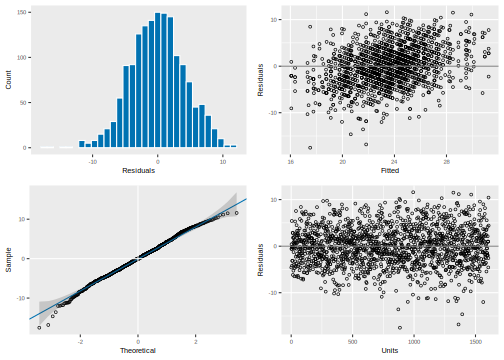
\includegraphics{wam_tuto_files/figure-latex/unnamed-chunk-122-1.pdf}
\caption{\label{fig:unnamed-chunk-122}Posterior trace and distribution for the fixed effects in model 2.2}
\end{figure}

As before we can obtain the raw variance component estimates and genetic correlations for the random effects:

\begin{Shaded}
\begin{Highlighting}[]
\KeywordTok{posterior.mode}\NormalTok{(model2}\FloatTok{.2}\OperatorTok{$}\NormalTok{VCV)}
\end{Highlighting}
\end{Shaded}

\begin{verbatim}
##       traitbwt:traitbwt.animal    traittarsus:traitbwt.animal 
##                      1.3294950                      2.0622374 
##    traitbwt:traittarsus.animal traittarsus:traittarsus.animal 
##                      2.0622374                      8.3900676 
##        traitbwt:traitbwt.byear     traittarsus:traitbwt.byear 
##                      0.8118565                      0.2327381 
##     traitbwt:traittarsus.byear  traittarsus:traittarsus.byear 
##                      0.2327381                      3.7375906 
##       traitbwt:traitbwt.mother    traittarsus:traitbwt.mother 
##                      1.4089440                     -1.4963686 
##    traitbwt:traittarsus.mother traittarsus:traittarsus.mother 
##                     -1.4963686                      3.9386669 
##        traitbwt:traitbwt.units     traittarsus:traitbwt.units 
##                      2.2353960                      4.3432849 
##     traitbwt:traittarsus.units  traittarsus:traittarsus.units 
##                      4.3432849                     15.0853981
\end{verbatim}

\begin{Shaded}
\begin{Highlighting}[]
\NormalTok{genetic.correlation2}\FloatTok{.2}\NormalTok{ \textless{}{-}}\StringTok{ }\NormalTok{model2}\FloatTok{.2}\OperatorTok{$}\NormalTok{VCV[, }\StringTok{"traitbwt:traittarsus.animal"}\NormalTok{] }\OperatorTok{/}\StringTok{ }\KeywordTok{sqrt}\NormalTok{(model2}\FloatTok{.2}\OperatorTok{$}\NormalTok{VCV[, }\StringTok{"traitbwt:traitbwt.animal"}\NormalTok{] }\OperatorTok{*}\StringTok{ }\NormalTok{model2}\FloatTok{.2}\OperatorTok{$}\NormalTok{VCV[, }\StringTok{"traittarsus:traittarsus.animal"}\NormalTok{])}
\NormalTok{maternal.correlation2}\FloatTok{.2}\NormalTok{ \textless{}{-}}\StringTok{ }\NormalTok{model2}\FloatTok{.2}\OperatorTok{$}\NormalTok{VCV[, }\StringTok{"traitbwt:traittarsus.mother"}\NormalTok{] }\OperatorTok{/}\StringTok{ }\KeywordTok{sqrt}\NormalTok{(model2}\FloatTok{.2}\OperatorTok{$}\NormalTok{VCV[, }\StringTok{"traitbwt:traitbwt.mother"}\NormalTok{] }\OperatorTok{*}\StringTok{ }\NormalTok{model2}\FloatTok{.2}\OperatorTok{$}\NormalTok{VCV[, }\StringTok{"traittarsus:traittarsus.mother"}\NormalTok{])}
\KeywordTok{posterior.mode}\NormalTok{(genetic.correlation2}\FloatTok{.2}\NormalTok{)}
\end{Highlighting}
\end{Shaded}

\begin{verbatim}
##      var1 
## 0.6932486
\end{verbatim}

\begin{Shaded}
\begin{Highlighting}[]
\KeywordTok{posterior.mode}\NormalTok{(maternal.correlation2}\FloatTok{.2}\NormalTok{)}
\end{Highlighting}
\end{Shaded}

\begin{verbatim}
##       var1 
## -0.7431221
\end{verbatim}

Evaluation of the statistical support for these genetic and maternal correlations is straightforward. Because we imposed no constraint on their estimation, we can evaluate the extent to which the posterior distributions overlap zero:

\begin{Shaded}
\begin{Highlighting}[]
\KeywordTok{HPDinterval}\NormalTok{(genetic.correlation2}\FloatTok{.2}\NormalTok{, }\FloatTok{0.95}\NormalTok{)}
\end{Highlighting}
\end{Shaded}

\begin{verbatim}
##          lower     upper
## var1 0.3062932 0.9197543
## attr(,"Probability")
## [1] 0.95
\end{verbatim}

\begin{Shaded}
\begin{Highlighting}[]
\KeywordTok{HPDinterval}\NormalTok{(maternal.correlation2}\FloatTok{.2}\NormalTok{, }\FloatTok{0.95}\NormalTok{)}
\end{Highlighting}
\end{Shaded}

\begin{verbatim}
##           lower      upper
## var1 -0.9432297 -0.3210149
## attr(,"Probability")
## [1] 0.95
\end{verbatim}

Neither or these posterior distributions overlaps zero, so we can consider them both statistically supported.

\hypertarget{direct-estimate-of-the-correlation-instead-of-the-covariance.}{%
\subsection{Direct estimate of the correlation instead of the covariance.}\label{direct-estimate-of-the-correlation-instead-of-the-covariance.}}

For this example, we just estimate the correlation at the genetic level, the covariance for the other random effect (\texttt{mother} and \texttt{byear}) and the residual level was not estimate to help the model to converge and compute faster. The prior will be the same but we change the \texttt{pr} argument to be \texttt{TRUE} to keep the posterior distribution of random effects.
To simplify the following code and facilitate the BLUP extraction, we rename the variable T1 and T2 and estimate correlation only for the additive genetic and residual matrices.

\begin{Shaded}
\begin{Highlighting}[]
\NormalTok{gryphon2}\OperatorTok{$}\NormalTok{T1 \textless{}{-}}\StringTok{ }\NormalTok{gryphon2}\OperatorTok{$}\NormalTok{bwt}
\NormalTok{gryphon2}\OperatorTok{$}\NormalTok{T2 \textless{}{-}}\StringTok{ }\NormalTok{gryphon2}\OperatorTok{$}\NormalTok{tarsus}
\CommentTok{\#}
\NormalTok{model2}\FloatTok{.3}\NormalTok{ \textless{}{-}}\StringTok{ }\KeywordTok{MCMCglmm}\NormalTok{(}\KeywordTok{cbind}\NormalTok{(T1, T2) }\OperatorTok{\textasciitilde{}}\StringTok{ }\NormalTok{trait }\OperatorTok{{-}}\StringTok{ }\DecValTok{1} \OperatorTok{+}\StringTok{ }\NormalTok{trait}\OperatorTok{:}\NormalTok{sex,}
  \DataTypeTok{random =} \OperatorTok{\textasciitilde{}}\StringTok{ }\KeywordTok{corg}\NormalTok{(trait)}\OperatorTok{:}\NormalTok{animal }\OperatorTok{+}\StringTok{ }\KeywordTok{corg}\NormalTok{(trait)}\OperatorTok{:}\NormalTok{byear }\OperatorTok{+}\StringTok{ }\KeywordTok{corg}\NormalTok{(trait)}\OperatorTok{:}\NormalTok{mother,}
  \DataTypeTok{rcov =} \OperatorTok{\textasciitilde{}}\StringTok{ }\KeywordTok{corg}\NormalTok{(trait)}\OperatorTok{:}\NormalTok{units,}
  \DataTypeTok{family =} \KeywordTok{c}\NormalTok{(}\StringTok{"gaussian"}\NormalTok{, }\StringTok{"gaussian"}\NormalTok{),}
  \DataTypeTok{ginv =} \KeywordTok{list}\NormalTok{(}\DataTypeTok{animal =}\NormalTok{ Ainv), }\DataTypeTok{data =}\NormalTok{ gryphon2,}
  \DataTypeTok{nitt =} \DecValTok{130000}\NormalTok{, }\DataTypeTok{thin =} \DecValTok{100}\NormalTok{, }\DataTypeTok{burnin =} \DecValTok{30000}\NormalTok{,}
  \DataTypeTok{prior =}\NormalTok{ prior2}\FloatTok{.2}\NormalTok{, }\DataTypeTok{verbose =} \OtherTok{FALSE}\NormalTok{, }\DataTypeTok{pr =} \OtherTok{TRUE}\NormalTok{,}
\NormalTok{)}

\KeywordTok{save}\NormalTok{(model2}\FloatTok{.3}\NormalTok{, }\DataTypeTok{file =} \StringTok{"data/MCMCglmm\_model2\_3\_LongRun.rda"}\NormalTok{)}
\end{Highlighting}
\end{Shaded}

Again we have provided the data from one such run. It can be accessed using the code:

\begin{Shaded}
\begin{Highlighting}[]
\KeywordTok{load}\NormalTok{(}\DataTypeTok{file =} \StringTok{"data/MCMCglmm\_model2\_3\_LongRun.rda"}\NormalTok{)}
\KeywordTok{summary}\NormalTok{(model2}\FloatTok{.3}\NormalTok{)}
\end{Highlighting}
\end{Shaded}

\begin{verbatim}
## 
##  Iterations = 30001:129901
##  Thinning interval  = 100
##  Sample size  = 1000 
## 
##  DIC: 972.9044 
## 
##  G-structure:  ~corg(trait):animal
## 
##                        post.mean l-95% CI u-95% CI eff.samp
## traitT1:traitT1.animal         1        1        1        0
## traitT2:traitT1.animal        -1       -1       -1        0
## traitT1:traitT2.animal        -1       -1       -1        0
## traitT2:traitT2.animal         1        1        1        0
## 
##                ~corg(trait):byear
## 
##                       post.mean l-95% CI u-95% CI eff.samp
## traitT1:traitT1.byear    1.0000  1.00000    1.000        0
## traitT2:traitT1.byear    0.2436 -0.09388    0.588     1000
## traitT1:traitT2.byear    0.2436 -0.09388    0.588     1000
## traitT2:traitT2.byear    1.0000  1.00000    1.000        0
## 
##                ~corg(trait):mother
## 
##                        post.mean l-95% CI u-95% CI eff.samp
## traitT1:traitT1.mother         1        1        1        0
## traitT2:traitT1.mother        -1       -1       -1        0
## traitT1:traitT2.mother        -1       -1       -1        0
## traitT2:traitT2.mother         1        1        1        0
## 
##  R-structure:  ~corg(trait):units
## 
##                       post.mean l-95% CI u-95% CI eff.samp
## traitT1:traitT1.units         1        1        1        0
## traitT2:traitT1.units         1        1        1        0
## traitT1:traitT2.units         1        1        1        0
## traitT2:traitT2.units         1        1        1        0
## 
##  Location effects: cbind(T1, T2) ~ trait - 1 + trait:sex 
## 
##              post.mean l-95% CI u-95% CI eff.samp  pMCMC    
## traitT1        6.29252  5.79418  6.77846     1000 <0.001 ***
## traitT2       20.53149 20.04183 21.00833     1000 <0.001 ***
## traitT1:sex2   2.07254  1.83815  2.32478     1000 <0.001 ***
## traitT2:sex2   0.02657 -0.21610  0.26411     1000  0.864    
## ---
## Signif. codes:  0 '***' 0.001 '**' 0.01 '*' 0.05 '.' 0.1 ' ' 1
\end{verbatim}

\begin{Shaded}
\begin{Highlighting}[]
\KeywordTok{autocorr}\NormalTok{(model2}\FloatTok{.3}\OperatorTok{$}\NormalTok{VCV)[, , }\StringTok{"traitT2:traitT1.animal"}\NormalTok{][}\DecValTok{3}\NormalTok{, }\DecValTok{4}\NormalTok{]}
\end{Highlighting}
\end{Shaded}

\begin{verbatim}
## [1] NaN
\end{verbatim}

Here we can plot the genetic correlation by extraction the breeding values or BLUP. Just to remember it is an example, the correlation is close to 1 due to a weak prior and model parameters.

\begin{Shaded}
\begin{Highlighting}[]
\NormalTok{DvsS \textless{}{-}}\StringTok{ }\KeywordTok{data.frame}\NormalTok{(}
  \DataTypeTok{Trait =} \KeywordTok{colnames}\NormalTok{(model2}\FloatTok{.3}\OperatorTok{$}\NormalTok{Sol),}
  \DataTypeTok{BLUP =} \KeywordTok{posterior.mode}\NormalTok{(model2}\FloatTok{.3}\OperatorTok{$}\NormalTok{Sol),}
  \DataTypeTok{CI =} \KeywordTok{HPDinterval}\NormalTok{((model2}\FloatTok{.3}\OperatorTok{$}\NormalTok{Sol))}
\NormalTok{)}
\NormalTok{DvsS \textless{}{-}}\StringTok{ }\NormalTok{DvsS[}\DecValTok{5}\OperatorTok{:}\DecValTok{2622}\NormalTok{, ] }\CommentTok{\# keep only rows associated with animal}

\NormalTok{DvsS}\OperatorTok{$}\NormalTok{ID \textless{}{-}}\StringTok{ }\KeywordTok{substr}\NormalTok{(DvsS}\OperatorTok{$}\NormalTok{Trait, }\DecValTok{16}\NormalTok{, }\DecValTok{19}\NormalTok{)}
\NormalTok{DvsS}\OperatorTok{$}\NormalTok{TRAIT \textless{}{-}}\StringTok{ }\KeywordTok{substr}\NormalTok{(DvsS}\OperatorTok{$}\NormalTok{Trait, }\DecValTok{6}\NormalTok{, }\DecValTok{7}\NormalTok{)}
\KeywordTok{summary}\NormalTok{(}\KeywordTok{factor}\NormalTok{(DvsS}\OperatorTok{$}\NormalTok{TRAIT))}
\end{Highlighting}
\end{Shaded}

\begin{verbatim}
##   T1   T2 
## 1309 1309
\end{verbatim}

\begin{Shaded}
\begin{Highlighting}[]
\NormalTok{DvsS}\OperatorTok{$}\NormalTok{Trait \textless{}{-}}\StringTok{ }\OtherTok{NULL}
\NormalTok{BLUPS \textless{}{-}}\StringTok{ }\KeywordTok{reshape}\NormalTok{(DvsS, }\DataTypeTok{v.names =} \KeywordTok{c}\NormalTok{(}\StringTok{"BLUP"}\NormalTok{, }\StringTok{"CI.lower"}\NormalTok{, }\StringTok{"CI.upper"}\NormalTok{), }\DataTypeTok{idvar =} \StringTok{"ID"}\NormalTok{, }\DataTypeTok{timevar =} \StringTok{"TRAIT"}\NormalTok{, }\DataTypeTok{direction =} \StringTok{"wide"}\NormalTok{)}
\KeywordTok{nrow}\NormalTok{(BLUPS)}
\end{Highlighting}
\end{Shaded}

\begin{verbatim}
## [1] 1309
\end{verbatim}

\begin{Shaded}
\begin{Highlighting}[]
\KeywordTok{rownames}\NormalTok{(BLUPS) \textless{}{-}}\StringTok{ }\KeywordTok{c}\NormalTok{()}
\KeywordTok{colnames}\NormalTok{(BLUPS) \textless{}{-}}\StringTok{ }\KeywordTok{c}\NormalTok{(}\StringTok{"ID"}\NormalTok{, }\StringTok{"BLUP.btw"}\NormalTok{, }\StringTok{"CI.L.btw"}\NormalTok{, }\StringTok{"CI.U.btw"}\NormalTok{, }\StringTok{"BLUP.tarsus"}\NormalTok{, }\StringTok{"CI.L.tarsus"}\NormalTok{, }\StringTok{"CI.U.tarsus"}\NormalTok{)}
\KeywordTok{summary}\NormalTok{(BLUPS)}
\end{Highlighting}
\end{Shaded}

\begin{verbatim}
##       ID               BLUP.btw           CI.L.btw          CI.U.btw      
##  Length:1309        Min.   :-3.92390   Min.   :-5.0229   Min.   :-3.0062  
##  Class :character   1st Qu.:-0.65954   1st Qu.:-2.1218   1st Qu.: 0.7462  
##  Mode  :character   Median : 0.01183   Median :-1.5472   Median : 1.5745  
##                     Mean   :-0.02007   Mean   :-1.4347   Mean   : 1.3860  
##                     3rd Qu.: 0.63842   3rd Qu.:-0.7509   3rd Qu.: 2.1033  
##                     Max.   : 3.78330   Max.   : 2.7030   Max.   : 4.7851  
##   BLUP.tarsus        CI.L.tarsus       CI.U.tarsus     
##  Min.   :-3.78353   Min.   :-4.6656   Min.   :-2.6778  
##  1st Qu.:-0.64453   1st Qu.:-2.1033   1st Qu.: 0.7505  
##  Median :-0.02336   Median :-1.5741   Median : 1.5477  
##  Mean   : 0.01820   Mean   :-1.3864   Mean   : 1.4343  
##  3rd Qu.: 0.65947   3rd Qu.:-0.7485   3rd Qu.: 2.1219  
##  Max.   : 3.93053   Max.   : 3.0061   Max.   : 5.0231
\end{verbatim}

\begin{Shaded}
\begin{Highlighting}[]
\CommentTok{\#}
\KeywordTok{par}\NormalTok{(}\DataTypeTok{mfrow =} \KeywordTok{c}\NormalTok{(}\DecValTok{2}\NormalTok{, }\DecValTok{2}\NormalTok{))}
\KeywordTok{hist}\NormalTok{(BLUPS}\OperatorTok{$}\NormalTok{BLUP.btw)}
\KeywordTok{qqnorm}\NormalTok{(BLUPS}\OperatorTok{$}\NormalTok{BLUP.btw)}
\KeywordTok{qqline}\NormalTok{(BLUPS}\OperatorTok{$}\NormalTok{BLUP.btw)}
\KeywordTok{hist}\NormalTok{(BLUPS}\OperatorTok{$}\NormalTok{BLUP.tarsus)}
\KeywordTok{qqnorm}\NormalTok{(BLUPS}\OperatorTok{$}\NormalTok{BLUP.tarsus)}
\KeywordTok{qqline}\NormalTok{(BLUPS}\OperatorTok{$}\NormalTok{BLUP.tarsus)}
\end{Highlighting}
\end{Shaded}

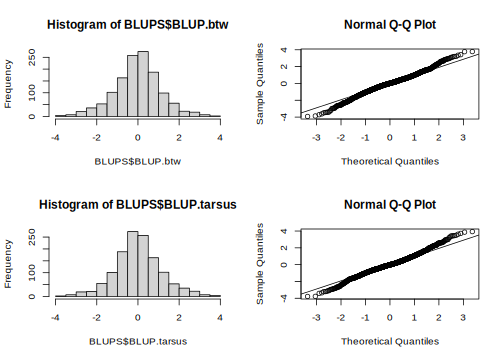
\includegraphics{wam_tuto_files/figure-latex/unnamed-chunk-127-1.pdf}

Here the code to plot the genetic correlation.

\begin{Shaded}
\begin{Highlighting}[]
\KeywordTok{plot}\NormalTok{(BLUP.tarsus }\OperatorTok{\textasciitilde{}}\StringTok{ }\NormalTok{BLUP.btw, BLUPS, }\DataTypeTok{xlab =} \StringTok{""}\NormalTok{, }\DataTypeTok{ylab =} \StringTok{""}\NormalTok{, }\DataTypeTok{las =} \FloatTok{1.2}\NormalTok{, }\DataTypeTok{bty =} \StringTok{"o"}\NormalTok{, }\DataTypeTok{col =} \StringTok{"white"}\NormalTok{, }\DataTypeTok{ylim =} \KeywordTok{c}\NormalTok{(}\OperatorTok{{-}}\DecValTok{4}\NormalTok{, }\DecValTok{4}\NormalTok{), }\DataTypeTok{xlim =} \KeywordTok{c}\NormalTok{(}\OperatorTok{{-}}\DecValTok{4}\NormalTok{, }\DecValTok{4}\NormalTok{))}
\KeywordTok{arrows}\NormalTok{(}\DataTypeTok{x0 =}\NormalTok{ BLUPS}\OperatorTok{$}\NormalTok{BLUP.btw, }\DataTypeTok{y0 =}\NormalTok{ BLUPS}\OperatorTok{$}\NormalTok{CI.L.tarsus, }\DataTypeTok{x1 =}\NormalTok{ BLUPS}\OperatorTok{$}\NormalTok{BLUP.btw, }\DataTypeTok{y1 =}\NormalTok{ BLUPS}\OperatorTok{$}\NormalTok{CI.U.tarsus, }\DataTypeTok{col =} \StringTok{"black"}\NormalTok{, }\DataTypeTok{code =} \DecValTok{3}\NormalTok{, }\DataTypeTok{angle =} \DecValTok{90}\NormalTok{, }\DataTypeTok{length =} \DecValTok{0}\NormalTok{)}
\KeywordTok{arrows}\NormalTok{(}\DataTypeTok{x0 =}\NormalTok{ BLUPS}\OperatorTok{$}\NormalTok{CI.L.btw, }\DataTypeTok{y0 =}\NormalTok{ BLUPS}\OperatorTok{$}\NormalTok{BLUP.tarsus, }\DataTypeTok{x1 =}\NormalTok{ BLUPS}\OperatorTok{$}\NormalTok{CI.U.btw, }\DataTypeTok{y1 =}\NormalTok{ BLUPS}\OperatorTok{$}\NormalTok{BLUP.tarsus, }\DataTypeTok{col =} \StringTok{"black"}\NormalTok{, }\DataTypeTok{code =} \DecValTok{3}\NormalTok{, }\DataTypeTok{angle =} \DecValTok{90}\NormalTok{, }\DataTypeTok{length =} \DecValTok{0}\NormalTok{)}
\KeywordTok{points}\NormalTok{(BLUP.tarsus }\OperatorTok{\textasciitilde{}}\StringTok{ }\NormalTok{BLUP.btw, BLUPS, }\DataTypeTok{pch =} \DecValTok{16}\NormalTok{, }\DataTypeTok{col =} \StringTok{"red"}\NormalTok{, }\DataTypeTok{cex =} \FloatTok{1.5}\NormalTok{)}
\KeywordTok{points}\NormalTok{(BLUP.tarsus }\OperatorTok{\textasciitilde{}}\StringTok{ }\NormalTok{BLUP.btw, BLUPS, }\DataTypeTok{pch =} \DecValTok{1}\NormalTok{, }\DataTypeTok{col =} \KeywordTok{rgb}\NormalTok{(}\DecValTok{0}\NormalTok{, }\DecValTok{0}\NormalTok{, }\DecValTok{0}\NormalTok{, }\FloatTok{0.3}\NormalTok{), }\DataTypeTok{cex =} \KeywordTok{c}\NormalTok{(}\FloatTok{1.5}\NormalTok{))}
\KeywordTok{mtext}\NormalTok{(}\StringTok{"btw (BV±SE)"}\NormalTok{, }\DataTypeTok{side =} \DecValTok{1}\NormalTok{, }\DataTypeTok{line =} \FloatTok{2.4}\NormalTok{)}
\KeywordTok{mtext}\NormalTok{(}\StringTok{"tarsus (BV±SE)"}\NormalTok{, }\DataTypeTok{side =} \DecValTok{2}\NormalTok{, }\DataTypeTok{line =} \DecValTok{2}\NormalTok{, }\DataTypeTok{las =} \DecValTok{3}\NormalTok{)}
\end{Highlighting}
\end{Shaded}

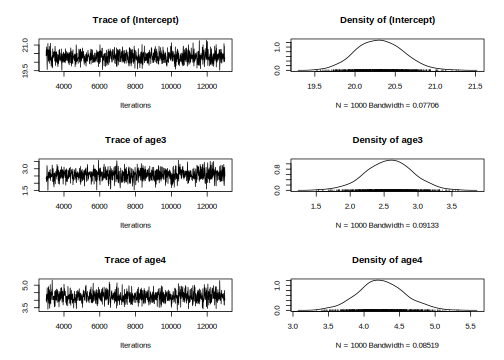
\includegraphics{wam_tuto_files/figure-latex/unnamed-chunk-128-1.pdf}

\hypertarget{partitioning-covariances}{%
\subsection{Partitioning (co)variances}\label{partitioning-covariances}}

As in the tutorial 1, it is possible to partition the variance-covariance matrix between groups (here sex)
Note: the model is simplified without sex-specific covariance for the \texttt{byear} and \texttt{mother} random effect.

\begin{Shaded}
\begin{Highlighting}[]
\NormalTok{gryphon2 \textless{}{-}}\StringTok{ }\NormalTok{gryphon2[}\KeywordTok{order}\NormalTok{(gryphon2}\OperatorTok{$}\NormalTok{sex), ]}


\NormalTok{prior2}\FloatTok{.3}\NormalTok{ \textless{}{-}}\StringTok{ }\KeywordTok{list}\NormalTok{(}
  \DataTypeTok{G =} \KeywordTok{list}\NormalTok{(}
    \DataTypeTok{G1 =} \KeywordTok{list}\NormalTok{(}\DataTypeTok{V =} \KeywordTok{diag}\NormalTok{(}\DecValTok{2}\NormalTok{), }\DataTypeTok{nu =} \FloatTok{1.002}\NormalTok{),}
    \DataTypeTok{G2 =} \KeywordTok{list}\NormalTok{(}\DataTypeTok{V =} \KeywordTok{diag}\NormalTok{(}\DecValTok{2}\NormalTok{), }\DataTypeTok{nu =} \FloatTok{1.002}\NormalTok{),}
    \DataTypeTok{G3 =} \KeywordTok{list}\NormalTok{(}\DataTypeTok{V =} \KeywordTok{diag}\NormalTok{(}\DecValTok{2}\NormalTok{), }\DataTypeTok{nu =} \FloatTok{1.002}\NormalTok{),}
    \DataTypeTok{G4 =} \KeywordTok{list}\NormalTok{(}\DataTypeTok{V =} \KeywordTok{diag}\NormalTok{(}\DecValTok{2}\NormalTok{), }\DataTypeTok{nu =} \FloatTok{1.002}\NormalTok{)}
\NormalTok{  ),}
  \DataTypeTok{R =} \KeywordTok{list}\NormalTok{(}
    \DataTypeTok{V1 =} \KeywordTok{list}\NormalTok{(}\DataTypeTok{V =} \KeywordTok{diag}\NormalTok{(}\DecValTok{2}\NormalTok{), }\DataTypeTok{nu =} \FloatTok{1.002}\NormalTok{),}
    \DataTypeTok{V2 =} \KeywordTok{list}\NormalTok{(}\DataTypeTok{V =} \KeywordTok{diag}\NormalTok{(}\DecValTok{2}\NormalTok{), }\DataTypeTok{nu =} \FloatTok{1.002}\NormalTok{)}
\NormalTok{  )}
\NormalTok{)}

\NormalTok{model2}\FloatTok{.4}\NormalTok{ \textless{}{-}}\StringTok{ }\KeywordTok{MCMCglmm}\NormalTok{(}\KeywordTok{cbind}\NormalTok{(bwt, tarsus) }\OperatorTok{\textasciitilde{}}\StringTok{ }\NormalTok{trait }\OperatorTok{{-}}\StringTok{ }\DecValTok{1} \OperatorTok{+}\StringTok{ }\NormalTok{trait}\OperatorTok{:}\NormalTok{sex,}
  \DataTypeTok{random =} \OperatorTok{\textasciitilde{}}\StringTok{ }\KeywordTok{us}\NormalTok{(}\KeywordTok{at.level}\NormalTok{(sex, }\StringTok{"1"}\NormalTok{)}\OperatorTok{:}\NormalTok{trait)}\OperatorTok{:}\NormalTok{animal }\OperatorTok{+}\StringTok{ }\KeywordTok{us}\NormalTok{(}\KeywordTok{at.level}\NormalTok{(sex, }\StringTok{"2"}\NormalTok{)}\OperatorTok{:}\NormalTok{trait)}\OperatorTok{:}\NormalTok{animal }\OperatorTok{+}\StringTok{ }\KeywordTok{idh}\NormalTok{(trait)}\OperatorTok{:}\NormalTok{byear }\OperatorTok{+}\StringTok{ }\KeywordTok{idh}\NormalTok{(trait)}\OperatorTok{:}\NormalTok{mother,}
  \DataTypeTok{rcov =} \OperatorTok{\textasciitilde{}}\StringTok{ }\KeywordTok{us}\NormalTok{(}\KeywordTok{at.level}\NormalTok{(sex, }\StringTok{"1"}\NormalTok{)}\OperatorTok{:}\NormalTok{trait)}\OperatorTok{:}\NormalTok{units }\OperatorTok{+}\StringTok{ }\KeywordTok{us}\NormalTok{(}\KeywordTok{at.level}\NormalTok{(sex, }\StringTok{"2"}\NormalTok{)}\OperatorTok{:}\NormalTok{trait)}\OperatorTok{:}\NormalTok{units,}
  \DataTypeTok{family =} \KeywordTok{c}\NormalTok{(}\StringTok{"gaussian"}\NormalTok{, }\StringTok{"gaussian"}\NormalTok{),}
  \DataTypeTok{ginv =} \KeywordTok{list}\NormalTok{(}\DataTypeTok{animal =}\NormalTok{ Ainv), }\DataTypeTok{data =}\NormalTok{ gryphon2,}
  \DataTypeTok{nitt =} \DecValTok{130000}\NormalTok{, }\DataTypeTok{thin =} \DecValTok{100}\NormalTok{, }\DataTypeTok{burnin =} \DecValTok{30000}\NormalTok{,}
  \DataTypeTok{prior =}\NormalTok{ prior2}\FloatTok{.3}\NormalTok{, }\DataTypeTok{verbose =} \OtherTok{FALSE}\NormalTok{, }\DataTypeTok{pr =} \OtherTok{TRUE}\NormalTok{,}
\NormalTok{)}
\KeywordTok{save}\NormalTok{(model2}\FloatTok{.4}\NormalTok{, }\DataTypeTok{file =} \StringTok{"data/MCMCglmm\_model2\_4\_LongRun.rda"}\NormalTok{)}
\end{Highlighting}
\end{Shaded}

Again we have provided the data from one such run. It can be accessed using the code:

\begin{Shaded}
\begin{Highlighting}[]
\KeywordTok{load}\NormalTok{(}\DataTypeTok{file =} \StringTok{"data/MCMCglmm\_model2\_4\_LongRun.rda"}\NormalTok{)}
\KeywordTok{summary}\NormalTok{(model2}\FloatTok{.4}\NormalTok{)}
\end{Highlighting}
\end{Shaded}

\begin{verbatim}
## 
##  Iterations = 30001:129901
##  Thinning interval  = 100
##  Sample size  = 1000 
## 
##  DIC: 5576.328 
## 
##  G-structure:  ~us(at.level(sex, "1"):trait):animal
## 
##                                                                      post.mean
## at.level(sex, "1"):traitbwt:at.level(sex, "1"):traitbwt.animal           1.122
## at.level(sex, "1"):traittarsus:at.level(sex, "1"):traitbwt.animal        1.127
## at.level(sex, "1"):traitbwt:at.level(sex, "1"):traittarsus.animal        1.127
## at.level(sex, "1"):traittarsus:at.level(sex, "1"):traittarsus.animal     3.379
##                                                                      l-95% CI
## at.level(sex, "1"):traitbwt:at.level(sex, "1"):traitbwt.animal         0.1602
## at.level(sex, "1"):traittarsus:at.level(sex, "1"):traitbwt.animal     -0.6531
## at.level(sex, "1"):traitbwt:at.level(sex, "1"):traittarsus.animal     -0.6531
## at.level(sex, "1"):traittarsus:at.level(sex, "1"):traittarsus.animal   0.1844
##                                                                      u-95% CI
## at.level(sex, "1"):traitbwt:at.level(sex, "1"):traitbwt.animal          2.359
## at.level(sex, "1"):traittarsus:at.level(sex, "1"):traitbwt.animal       3.496
## at.level(sex, "1"):traitbwt:at.level(sex, "1"):traittarsus.animal       3.496
## at.level(sex, "1"):traittarsus:at.level(sex, "1"):traittarsus.animal    8.918
##                                                                      eff.samp
## at.level(sex, "1"):traitbwt:at.level(sex, "1"):traitbwt.animal          167.5
## at.level(sex, "1"):traittarsus:at.level(sex, "1"):traitbwt.animal       119.3
## at.level(sex, "1"):traitbwt:at.level(sex, "1"):traittarsus.animal       119.3
## at.level(sex, "1"):traittarsus:at.level(sex, "1"):traittarsus.animal    102.6
## 
##                ~us(at.level(sex, "2"):trait):animal
## 
##                                                                      post.mean
## at.level(sex, "2"):traitbwt:at.level(sex, "2"):traitbwt.animal           1.598
## at.level(sex, "2"):traittarsus:at.level(sex, "2"):traitbwt.animal        3.099
## at.level(sex, "2"):traitbwt:at.level(sex, "2"):traittarsus.animal        3.099
## at.level(sex, "2"):traittarsus:at.level(sex, "2"):traittarsus.animal    10.218
##                                                                      l-95% CI
## at.level(sex, "2"):traitbwt:at.level(sex, "2"):traitbwt.animal         0.1895
## at.level(sex, "2"):traittarsus:at.level(sex, "2"):traitbwt.animal     -0.5506
## at.level(sex, "2"):traitbwt:at.level(sex, "2"):traittarsus.animal     -0.5506
## at.level(sex, "2"):traittarsus:at.level(sex, "2"):traittarsus.animal   0.2127
##                                                                      u-95% CI
## at.level(sex, "2"):traitbwt:at.level(sex, "2"):traitbwt.animal          3.305
## at.level(sex, "2"):traittarsus:at.level(sex, "2"):traitbwt.animal       7.864
## at.level(sex, "2"):traitbwt:at.level(sex, "2"):traittarsus.animal       7.864
## at.level(sex, "2"):traittarsus:at.level(sex, "2"):traittarsus.animal   24.230
##                                                                      eff.samp
## at.level(sex, "2"):traitbwt:at.level(sex, "2"):traitbwt.animal          57.28
## at.level(sex, "2"):traittarsus:at.level(sex, "2"):traitbwt.animal       42.01
## at.level(sex, "2"):traitbwt:at.level(sex, "2"):traittarsus.animal       42.01
## at.level(sex, "2"):traittarsus:at.level(sex, "2"):traittarsus.animal    37.21
## 
##                ~idh(trait):byear
## 
##                   post.mean l-95% CI u-95% CI eff.samp
## traitbwt.byear       0.9309   0.4614    1.463     1000
## traittarsus.byear    4.0310   1.9268    6.724     1000
## 
##                ~idh(trait):mother
## 
##                    post.mean l-95% CI u-95% CI eff.samp
## traitbwt.mother        1.924    1.406    2.398    667.6
## traittarsus.mother     7.093    4.626    9.681    698.5
## 
##  R-structure:  ~us(at.level(sex, "1"):trait):units
## 
##                                                                     post.mean
## at.level(sex, "1"):traitbwt:at.level(sex, "1"):traitbwt.units           2.090
## at.level(sex, "1"):traittarsus:at.level(sex, "1"):traitbwt.units        4.533
## at.level(sex, "1"):traitbwt:at.level(sex, "1"):traittarsus.units        4.533
## at.level(sex, "1"):traittarsus:at.level(sex, "1"):traittarsus.units    14.113
##                                                                     l-95% CI
## at.level(sex, "1"):traitbwt:at.level(sex, "1"):traitbwt.units         0.9958
## at.level(sex, "1"):traittarsus:at.level(sex, "1"):traitbwt.units      2.4185
## at.level(sex, "1"):traitbwt:at.level(sex, "1"):traittarsus.units      2.4185
## at.level(sex, "1"):traittarsus:at.level(sex, "1"):traittarsus.units   8.1848
##                                                                     u-95% CI
## at.level(sex, "1"):traitbwt:at.level(sex, "1"):traitbwt.units          3.128
## at.level(sex, "1"):traittarsus:at.level(sex, "1"):traitbwt.units       6.875
## at.level(sex, "1"):traitbwt:at.level(sex, "1"):traittarsus.units       6.875
## at.level(sex, "1"):traittarsus:at.level(sex, "1"):traittarsus.units   18.935
##                                                                     eff.samp
## at.level(sex, "1"):traitbwt:at.level(sex, "1"):traitbwt.units          207.2
## at.level(sex, "1"):traittarsus:at.level(sex, "1"):traitbwt.units       168.4
## at.level(sex, "1"):traitbwt:at.level(sex, "1"):traittarsus.units       168.4
## at.level(sex, "1"):traittarsus:at.level(sex, "1"):traittarsus.units    185.3
## 
##                ~us(at.level(sex, "2"):trait):units
## 
##                                                                     post.mean
## at.level(sex, "2"):traitbwt:at.level(sex, "2"):traitbwt.units           1.782
## at.level(sex, "2"):traittarsus:at.level(sex, "2"):traitbwt.units        3.697
## at.level(sex, "2"):traitbwt:at.level(sex, "2"):traittarsus.units        3.697
## at.level(sex, "2"):traittarsus:at.level(sex, "2"):traittarsus.units    12.437
##                                                                     l-95% CI
## at.level(sex, "2"):traitbwt:at.level(sex, "2"):traitbwt.units         0.2776
## at.level(sex, "2"):traittarsus:at.level(sex, "2"):traitbwt.units     -0.3141
## at.level(sex, "2"):traitbwt:at.level(sex, "2"):traittarsus.units     -0.3141
## at.level(sex, "2"):traittarsus:at.level(sex, "2"):traittarsus.units   0.1776
##                                                                     u-95% CI
## at.level(sex, "2"):traitbwt:at.level(sex, "2"):traitbwt.units          3.115
## at.level(sex, "2"):traittarsus:at.level(sex, "2"):traitbwt.units       7.218
## at.level(sex, "2"):traitbwt:at.level(sex, "2"):traittarsus.units       7.218
## at.level(sex, "2"):traittarsus:at.level(sex, "2"):traittarsus.units   21.903
##                                                                     eff.samp
## at.level(sex, "2"):traitbwt:at.level(sex, "2"):traitbwt.units          52.55
## at.level(sex, "2"):traittarsus:at.level(sex, "2"):traitbwt.units       51.90
## at.level(sex, "2"):traitbwt:at.level(sex, "2"):traittarsus.units       51.90
## at.level(sex, "2"):traittarsus:at.level(sex, "2"):traittarsus.units    39.20
## 
##  Location effects: cbind(bwt, tarsus) ~ trait - 1 + trait:sex 
## 
##                  post.mean l-95% CI u-95% CI eff.samp  pMCMC    
## traitbwt           6.30098  5.89218  6.78834   1000.0 <0.001 ***
## traittarsus       20.45577 19.53577 21.34719   1129.8 <0.001 ***
## traitbwt:sex2      2.01306  1.63662  2.38011    887.4 <0.001 ***
## traittarsus:sex2   0.05817 -0.86635  0.89119   1016.6  0.896    
## ---
## Signif. codes:  0 '***' 0.001 '**' 0.01 '*' 0.05 '.' 0.1 ' ' 1
\end{verbatim}

\begin{Shaded}
\begin{Highlighting}[]
\KeywordTok{autocorr}\NormalTok{(model2}\FloatTok{.4}\OperatorTok{$}\NormalTok{VCV)}
\end{Highlighting}
\end{Shaded}

\begin{verbatim}
## , , at.level(sex, "1"):traitbwt:at.level(sex, "1"):traitbwt.animal
## 
##          at.level(sex, "1"):traitbwt:at.level(sex, "1"):traitbwt.animal
## Lag 0                                                        1.00000000
## Lag 100                                                      0.64694479
## Lag 500                                                      0.18648179
## Lag 1000                                                     0.10392219
## Lag 5000                                                    -0.04275072
##          at.level(sex, "1"):traittarsus:at.level(sex, "1"):traitbwt.animal
## Lag 0                                                           0.84704874
## Lag 100                                                         0.60161240
## Lag 500                                                         0.20180692
## Lag 1000                                                        0.10068129
## Lag 5000                                                       -0.03878312
##          at.level(sex, "1"):traitbwt:at.level(sex, "1"):traittarsus.animal
## Lag 0                                                           0.84704874
## Lag 100                                                         0.60161240
## Lag 500                                                         0.20180692
## Lag 1000                                                        0.10068129
## Lag 5000                                                       -0.03878312
##          at.level(sex, "1"):traittarsus:at.level(sex, "1"):traittarsus.animal
## Lag 0                                                              0.53041407
## Lag 100                                                            0.39413485
## Lag 500                                                            0.16964194
## Lag 1000                                                           0.11264314
## Lag 5000                                                          -0.01013697
##          at.level(sex, "2"):traitbwt:at.level(sex, "2"):traitbwt.animal
## Lag 0                                                       -0.07132000
## Lag 100                                                     -0.09608251
## Lag 500                                                     -0.05360431
## Lag 1000                                                    -0.02600414
## Lag 5000                                                    -0.02326421
##          at.level(sex, "2"):traittarsus:at.level(sex, "2"):traitbwt.animal
## Lag 0                                                          -0.07404287
## Lag 100                                                        -0.08742103
## Lag 500                                                        -0.05376905
## Lag 1000                                                       -0.03219125
## Lag 5000                                                        0.02771727
##          at.level(sex, "2"):traitbwt:at.level(sex, "2"):traittarsus.animal
## Lag 0                                                          -0.07404287
## Lag 100                                                        -0.08742103
## Lag 500                                                        -0.05376905
## Lag 1000                                                       -0.03219125
## Lag 5000                                                        0.02771727
##          at.level(sex, "2"):traittarsus:at.level(sex, "2"):traittarsus.animal
## Lag 0                                                             -0.06663301
## Lag 100                                                           -0.07398282
## Lag 500                                                           -0.03873715
## Lag 1000                                                          -0.03346102
## Lag 5000                                                           0.06535632
##          traitbwt.byear traittarsus.byear traitbwt.mother traittarsus.mother
## Lag 0      -0.002044905        0.06061428     -0.13681757        0.063034744
## Lag 100    -0.029101625        0.04741082     -0.09232454        0.062553003
## Lag 500    -0.025891155        0.04101237     -0.01510511       -0.026837884
## Lag 1000    0.029398462        0.02792539     -0.02514900        0.009578198
## Lag 5000   -0.016122661        0.03081539      0.04189460       -0.039791141
##          at.level(sex, "1"):traitbwt:at.level(sex, "1"):traitbwt.units
## Lag 0                                                     -0.842319278
## Lag 100                                                   -0.569203867
## Lag 500                                                   -0.167844469
## Lag 1000                                                  -0.114647645
## Lag 5000                                                  -0.002132053
##          at.level(sex, "1"):traittarsus:at.level(sex, "1"):traitbwt.units
## Lag 0                                                        -0.708901550
## Lag 100                                                      -0.517998161
## Lag 500                                                      -0.167589741
## Lag 1000                                                     -0.110500558
## Lag 5000                                                      0.002914291
##          at.level(sex, "1"):traitbwt:at.level(sex, "1"):traittarsus.units
## Lag 0                                                        -0.708901550
## Lag 100                                                      -0.517998161
## Lag 500                                                      -0.167589741
## Lag 1000                                                     -0.110500558
## Lag 5000                                                      0.002914291
##          at.level(sex, "1"):traittarsus:at.level(sex, "1"):traittarsus.units
## Lag 0                                                           -0.438123204
## Lag 100                                                         -0.337083166
## Lag 500                                                         -0.129292647
## Lag 1000                                                        -0.103678560
## Lag 5000                                                        -0.001926232
##          at.level(sex, "2"):traitbwt:at.level(sex, "2"):traitbwt.units
## Lag 0                                                       0.07807105
## Lag 100                                                     0.10707885
## Lag 500                                                     0.05568856
## Lag 1000                                                    0.02521629
## Lag 5000                                                    0.01402475
##          at.level(sex, "2"):traittarsus:at.level(sex, "2"):traitbwt.units
## Lag 0                                                          0.06679340
## Lag 100                                                        0.08704308
## Lag 500                                                        0.05892190
## Lag 1000                                                       0.02676188
## Lag 5000                                                      -0.03056683
##          at.level(sex, "2"):traitbwt:at.level(sex, "2"):traittarsus.units
## Lag 0                                                          0.06679340
## Lag 100                                                        0.08704308
## Lag 500                                                        0.05892190
## Lag 1000                                                       0.02676188
## Lag 5000                                                      -0.03056683
##          at.level(sex, "2"):traittarsus:at.level(sex, "2"):traittarsus.units
## Lag 0                                                             0.04797898
## Lag 100                                                           0.05730717
## Lag 500                                                           0.04727555
## Lag 1000                                                          0.02677473
## Lag 5000                                                         -0.06608227
## 
## , , at.level(sex, "1"):traittarsus:at.level(sex, "1"):traitbwt.animal
## 
##          at.level(sex, "1"):traitbwt:at.level(sex, "1"):traitbwt.animal
## Lag 0                                                       0.847048735
## Lag 100                                                     0.596411029
## Lag 500                                                     0.228550625
## Lag 1000                                                    0.137616124
## Lag 5000                                                    0.009429906
##          at.level(sex, "1"):traittarsus:at.level(sex, "1"):traitbwt.animal
## Lag 0                                                           1.00000000
## Lag 100                                                         0.71730236
## Lag 500                                                         0.27616079
## Lag 1000                                                        0.13795063
## Lag 5000                                                        0.01144749
##          at.level(sex, "1"):traitbwt:at.level(sex, "1"):traittarsus.animal
## Lag 0                                                           1.00000000
## Lag 100                                                         0.71730236
## Lag 500                                                         0.27616079
## Lag 1000                                                        0.13795063
## Lag 5000                                                        0.01144749
##          at.level(sex, "1"):traittarsus:at.level(sex, "1"):traittarsus.animal
## Lag 0                                                               0.7989970
## Lag 100                                                             0.6014134
## Lag 500                                                             0.2515262
## Lag 1000                                                            0.1354306
## Lag 5000                                                            0.0136445
##          at.level(sex, "2"):traitbwt:at.level(sex, "2"):traitbwt.animal
## Lag 0                                                      -0.069644149
## Lag 100                                                    -0.094348331
## Lag 500                                                    -0.069174874
## Lag 1000                                                   -0.030980734
## Lag 5000                                                   -0.001770693
##          at.level(sex, "2"):traittarsus:at.level(sex, "2"):traitbwt.animal
## Lag 0                                                          -0.09266557
## Lag 100                                                        -0.10417316
## Lag 500                                                        -0.06908668
## Lag 1000                                                       -0.04934221
## Lag 5000                                                        0.03968797
##          at.level(sex, "2"):traitbwt:at.level(sex, "2"):traittarsus.animal
## Lag 0                                                          -0.09266557
## Lag 100                                                        -0.10417316
## Lag 500                                                        -0.06908668
## Lag 1000                                                       -0.04934221
## Lag 5000                                                        0.03968797
##          at.level(sex, "2"):traittarsus:at.level(sex, "2"):traittarsus.animal
## Lag 0                                                             -0.10219567
## Lag 100                                                           -0.10740690
## Lag 500                                                           -0.05829130
## Lag 1000                                                          -0.05667648
## Lag 5000                                                           0.08311412
##          traitbwt.byear traittarsus.byear traitbwt.mother traittarsus.mother
## Lag 0       -0.03731153        0.05572330     -0.12626725         0.06865980
## Lag 100     -0.04492620        0.05076637     -0.08142219         0.05404288
## Lag 500     -0.03460527        0.03246607     -0.03107773        -0.02899561
## Lag 1000     0.01459594        0.01717445     -0.05078674         0.01110690
## Lag 5000    -0.01688700        0.03883380      0.02698184        -0.03307579
##          at.level(sex, "1"):traitbwt:at.level(sex, "1"):traitbwt.units
## Lag 0                                                      -0.73143141
## Lag 100                                                    -0.52689086
## Lag 500                                                    -0.22551523
## Lag 1000                                                   -0.12616708
## Lag 5000                                                   -0.04647821
##          at.level(sex, "1"):traittarsus:at.level(sex, "1"):traitbwt.units
## Lag 0                                                         -0.82495927
## Lag 100                                                       -0.60990914
## Lag 500                                                       -0.24464022
## Lag 1000                                                      -0.12721295
## Lag 5000                                                      -0.03841367
##          at.level(sex, "1"):traitbwt:at.level(sex, "1"):traittarsus.units
## Lag 0                                                         -0.82495927
## Lag 100                                                       -0.60990914
## Lag 500                                                       -0.24464022
## Lag 1000                                                      -0.12721295
## Lag 5000                                                      -0.03841367
##          at.level(sex, "1"):traittarsus:at.level(sex, "1"):traittarsus.units
## Lag 0                                                            -0.64394327
## Lag 100                                                          -0.48995337
## Lag 500                                                          -0.19725633
## Lag 1000                                                         -0.10852446
## Lag 5000                                                         -0.02105523
##          at.level(sex, "2"):traitbwt:at.level(sex, "2"):traitbwt.units
## Lag 0                                                      0.082481767
## Lag 100                                                    0.105417000
## Lag 500                                                    0.073280263
## Lag 1000                                                   0.028355398
## Lag 5000                                                  -0.006019758
##          at.level(sex, "2"):traittarsus:at.level(sex, "2"):traitbwt.units
## Lag 0                                                          0.09308370
## Lag 100                                                        0.10680733
## Lag 500                                                        0.07810010
## Lag 1000                                                       0.04359553
## Lag 5000                                                      -0.04726853
##          at.level(sex, "2"):traitbwt:at.level(sex, "2"):traittarsus.units
## Lag 0                                                          0.09308370
## Lag 100                                                        0.10680733
## Lag 500                                                        0.07810010
## Lag 1000                                                       0.04359553
## Lag 5000                                                      -0.04726853
##          at.level(sex, "2"):traittarsus:at.level(sex, "2"):traittarsus.units
## Lag 0                                                             0.08843633
## Lag 100                                                           0.09343376
## Lag 500                                                           0.06886426
## Lag 1000                                                          0.05338682
## Lag 5000                                                         -0.09185034
## 
## , , at.level(sex, "1"):traitbwt:at.level(sex, "1"):traittarsus.animal
## 
##          at.level(sex, "1"):traitbwt:at.level(sex, "1"):traitbwt.animal
## Lag 0                                                       0.847048735
## Lag 100                                                     0.596411029
## Lag 500                                                     0.228550625
## Lag 1000                                                    0.137616124
## Lag 5000                                                    0.009429906
##          at.level(sex, "1"):traittarsus:at.level(sex, "1"):traitbwt.animal
## Lag 0                                                           1.00000000
## Lag 100                                                         0.71730236
## Lag 500                                                         0.27616079
## Lag 1000                                                        0.13795063
## Lag 5000                                                        0.01144749
##          at.level(sex, "1"):traitbwt:at.level(sex, "1"):traittarsus.animal
## Lag 0                                                           1.00000000
## Lag 100                                                         0.71730236
## Lag 500                                                         0.27616079
## Lag 1000                                                        0.13795063
## Lag 5000                                                        0.01144749
##          at.level(sex, "1"):traittarsus:at.level(sex, "1"):traittarsus.animal
## Lag 0                                                               0.7989970
## Lag 100                                                             0.6014134
## Lag 500                                                             0.2515262
## Lag 1000                                                            0.1354306
## Lag 5000                                                            0.0136445
##          at.level(sex, "2"):traitbwt:at.level(sex, "2"):traitbwt.animal
## Lag 0                                                      -0.069644149
## Lag 100                                                    -0.094348331
## Lag 500                                                    -0.069174874
## Lag 1000                                                   -0.030980734
## Lag 5000                                                   -0.001770693
##          at.level(sex, "2"):traittarsus:at.level(sex, "2"):traitbwt.animal
## Lag 0                                                          -0.09266557
## Lag 100                                                        -0.10417316
## Lag 500                                                        -0.06908668
## Lag 1000                                                       -0.04934221
## Lag 5000                                                        0.03968797
##          at.level(sex, "2"):traitbwt:at.level(sex, "2"):traittarsus.animal
## Lag 0                                                          -0.09266557
## Lag 100                                                        -0.10417316
## Lag 500                                                        -0.06908668
## Lag 1000                                                       -0.04934221
## Lag 5000                                                        0.03968797
##          at.level(sex, "2"):traittarsus:at.level(sex, "2"):traittarsus.animal
## Lag 0                                                             -0.10219567
## Lag 100                                                           -0.10740690
## Lag 500                                                           -0.05829130
## Lag 1000                                                          -0.05667648
## Lag 5000                                                           0.08311412
##          traitbwt.byear traittarsus.byear traitbwt.mother traittarsus.mother
## Lag 0       -0.03731153        0.05572330     -0.12626725         0.06865980
## Lag 100     -0.04492620        0.05076637     -0.08142219         0.05404288
## Lag 500     -0.03460527        0.03246607     -0.03107773        -0.02899561
## Lag 1000     0.01459594        0.01717445     -0.05078674         0.01110690
## Lag 5000    -0.01688700        0.03883380      0.02698184        -0.03307579
##          at.level(sex, "1"):traitbwt:at.level(sex, "1"):traitbwt.units
## Lag 0                                                      -0.73143141
## Lag 100                                                    -0.52689086
## Lag 500                                                    -0.22551523
## Lag 1000                                                   -0.12616708
## Lag 5000                                                   -0.04647821
##          at.level(sex, "1"):traittarsus:at.level(sex, "1"):traitbwt.units
## Lag 0                                                         -0.82495927
## Lag 100                                                       -0.60990914
## Lag 500                                                       -0.24464022
## Lag 1000                                                      -0.12721295
## Lag 5000                                                      -0.03841367
##          at.level(sex, "1"):traitbwt:at.level(sex, "1"):traittarsus.units
## Lag 0                                                         -0.82495927
## Lag 100                                                       -0.60990914
## Lag 500                                                       -0.24464022
## Lag 1000                                                      -0.12721295
## Lag 5000                                                      -0.03841367
##          at.level(sex, "1"):traittarsus:at.level(sex, "1"):traittarsus.units
## Lag 0                                                            -0.64394327
## Lag 100                                                          -0.48995337
## Lag 500                                                          -0.19725633
## Lag 1000                                                         -0.10852446
## Lag 5000                                                         -0.02105523
##          at.level(sex, "2"):traitbwt:at.level(sex, "2"):traitbwt.units
## Lag 0                                                      0.082481767
## Lag 100                                                    0.105417000
## Lag 500                                                    0.073280263
## Lag 1000                                                   0.028355398
## Lag 5000                                                  -0.006019758
##          at.level(sex, "2"):traittarsus:at.level(sex, "2"):traitbwt.units
## Lag 0                                                          0.09308370
## Lag 100                                                        0.10680733
## Lag 500                                                        0.07810010
## Lag 1000                                                       0.04359553
## Lag 5000                                                      -0.04726853
##          at.level(sex, "2"):traitbwt:at.level(sex, "2"):traittarsus.units
## Lag 0                                                          0.09308370
## Lag 100                                                        0.10680733
## Lag 500                                                        0.07810010
## Lag 1000                                                       0.04359553
## Lag 5000                                                      -0.04726853
##          at.level(sex, "2"):traittarsus:at.level(sex, "2"):traittarsus.units
## Lag 0                                                             0.08843633
## Lag 100                                                           0.09343376
## Lag 500                                                           0.06886426
## Lag 1000                                                          0.05338682
## Lag 5000                                                         -0.09185034
## 
## , , at.level(sex, "1"):traittarsus:at.level(sex, "1"):traittarsus.animal
## 
##          at.level(sex, "1"):traitbwt:at.level(sex, "1"):traitbwt.animal
## Lag 0                                                         0.5304141
## Lag 100                                                       0.3737195
## Lag 500                                                       0.1441203
## Lag 1000                                                      0.1503417
## Lag 5000                                                      0.1187940
##          at.level(sex, "1"):traittarsus:at.level(sex, "1"):traitbwt.animal
## Lag 0                                                            0.7989970
## Lag 100                                                          0.5706521
## Lag 500                                                          0.2430451
## Lag 1000                                                         0.1680830
## Lag 5000                                                         0.1259980
##          at.level(sex, "1"):traitbwt:at.level(sex, "1"):traittarsus.animal
## Lag 0                                                            0.7989970
## Lag 100                                                          0.5706521
## Lag 500                                                          0.2430451
## Lag 1000                                                         0.1680830
## Lag 5000                                                         0.1259980
##          at.level(sex, "1"):traittarsus:at.level(sex, "1"):traittarsus.animal
## Lag 0                                                              1.00000000
## Lag 100                                                            0.73196692
## Lag 500                                                            0.31335783
## Lag 1000                                                           0.18501263
## Lag 5000                                                           0.08438218
##          at.level(sex, "2"):traitbwt:at.level(sex, "2"):traitbwt.animal
## Lag 0                                                       -0.01785209
## Lag 100                                                     -0.03508025
## Lag 500                                                     -0.04733762
## Lag 1000                                                    -0.01709422
## Lag 5000                                                    -0.01586047
##          at.level(sex, "2"):traittarsus:at.level(sex, "2"):traitbwt.animal
## Lag 0                                                         -0.038020441
## Lag 100                                                       -0.045171003
## Lag 500                                                       -0.050004069
## Lag 1000                                                      -0.054183547
## Lag 5000                                                      -0.004955516
##          at.level(sex, "2"):traitbwt:at.level(sex, "2"):traittarsus.animal
## Lag 0                                                         -0.038020441
## Lag 100                                                       -0.045171003
## Lag 500                                                       -0.050004069
## Lag 1000                                                      -0.054183547
## Lag 5000                                                      -0.004955516
##          at.level(sex, "2"):traittarsus:at.level(sex, "2"):traittarsus.animal
## Lag 0                                                             -0.05447207
## Lag 100                                                           -0.05998184
## Lag 500                                                           -0.06158778
## Lag 1000                                                          -0.08267333
## Lag 5000                                                           0.02065741
##          traitbwt.byear traittarsus.byear traitbwt.mother traittarsus.mother
## Lag 0      -0.060159939        0.06450755   -0.0973321863       -0.009350685
## Lag 100    -0.043720033        0.03483594   -0.0765923141       -0.006212912
## Lag 500    -0.052466217        0.02987272   -0.0662772868       -0.030465249
## Lag 1000   -0.001034192        0.03110963   -0.0728720391        0.009855596
## Lag 5000   -0.034160786        0.05472996    0.0008533055        0.003426058
##          at.level(sex, "1"):traitbwt:at.level(sex, "1"):traitbwt.units
## Lag 0                                                       -0.4637838
## Lag 100                                                     -0.3337342
## Lag 500                                                     -0.1618186
## Lag 1000                                                    -0.1329387
## Lag 5000                                                    -0.1239580
##          at.level(sex, "1"):traittarsus:at.level(sex, "1"):traitbwt.units
## Lag 0                                                          -0.6583252
## Lag 100                                                        -0.4881849
## Lag 500                                                        -0.2287167
## Lag 1000                                                       -0.1381960
## Lag 5000                                                       -0.1179873
##          at.level(sex, "1"):traitbwt:at.level(sex, "1"):traittarsus.units
## Lag 0                                                          -0.6583252
## Lag 100                                                        -0.4881849
## Lag 500                                                        -0.2287167
## Lag 1000                                                       -0.1381960
## Lag 5000                                                       -0.1179873
##          at.level(sex, "1"):traittarsus:at.level(sex, "1"):traittarsus.units
## Lag 0                                                            -0.76001059
## Lag 100                                                          -0.57358014
## Lag 500                                                          -0.25179771
## Lag 1000                                                         -0.12123408
## Lag 5000                                                         -0.07986147
##          at.level(sex, "2"):traitbwt:at.level(sex, "2"):traitbwt.units
## Lag 0                                                       0.02870904
## Lag 100                                                     0.03399695
## Lag 500                                                     0.05485675
## Lag 1000                                                    0.01651664
## Lag 5000                                                    0.01516504
##          at.level(sex, "2"):traittarsus:at.level(sex, "2"):traitbwt.units
## Lag 0                                                         0.039633904
## Lag 100                                                       0.041502118
## Lag 500                                                       0.059018043
## Lag 1000                                                      0.052958967
## Lag 5000                                                     -0.002274568
##          at.level(sex, "2"):traitbwt:at.level(sex, "2"):traittarsus.units
## Lag 0                                                         0.039633904
## Lag 100                                                       0.041502118
## Lag 500                                                       0.059018043
## Lag 1000                                                      0.052958967
## Lag 5000                                                     -0.002274568
##          at.level(sex, "2"):traittarsus:at.level(sex, "2"):traittarsus.units
## Lag 0                                                             0.04584246
## Lag 100                                                           0.04763329
## Lag 500                                                           0.06852725
## Lag 1000                                                          0.08362165
## Lag 5000                                                         -0.03430204
## 
## , , at.level(sex, "2"):traitbwt:at.level(sex, "2"):traitbwt.animal
## 
##          at.level(sex, "1"):traitbwt:at.level(sex, "1"):traitbwt.animal
## Lag 0                                                       -0.07132000
## Lag 100                                                     -0.06108550
## Lag 500                                                     -0.06344456
## Lag 1000                                                    -0.02628413
## Lag 5000                                                     0.10351490
##          at.level(sex, "1"):traittarsus:at.level(sex, "1"):traitbwt.animal
## Lag 0                                                        -0.0696441487
## Lag 100                                                      -0.0685711479
## Lag 500                                                      -0.0543839240
## Lag 1000                                                      0.0004950661
## Lag 5000                                                      0.1221823016
##          at.level(sex, "1"):traitbwt:at.level(sex, "1"):traittarsus.animal
## Lag 0                                                        -0.0696441487
## Lag 100                                                      -0.0685711479
## Lag 500                                                      -0.0543839240
## Lag 1000                                                      0.0004950661
## Lag 5000                                                      0.1221823016
##          at.level(sex, "1"):traittarsus:at.level(sex, "1"):traittarsus.animal
## Lag 0                                                           -0.0178520882
## Lag 100                                                         -0.0173974776
## Lag 500                                                         -0.0002494694
## Lag 1000                                                         0.0551913450
## Lag 5000                                                         0.1333840825
##          at.level(sex, "2"):traitbwt:at.level(sex, "2"):traitbwt.animal
## Lag 0                                                         1.0000000
## Lag 100                                                       0.8242352
## Lag 500                                                       0.5296802
## Lag 1000                                                      0.3040607
## Lag 5000                                                     -0.1276161
##          at.level(sex, "2"):traittarsus:at.level(sex, "2"):traitbwt.animal
## Lag 0                                                            0.9099634
## Lag 100                                                          0.8047694
## Lag 500                                                          0.5857973
## Lag 1000                                                         0.3552775
## Lag 5000                                                        -0.1485103
##          at.level(sex, "2"):traitbwt:at.level(sex, "2"):traittarsus.animal
## Lag 0                                                            0.9099634
## Lag 100                                                          0.8047694
## Lag 500                                                          0.5857973
## Lag 1000                                                         0.3552775
## Lag 5000                                                        -0.1485103
##          at.level(sex, "2"):traittarsus:at.level(sex, "2"):traittarsus.animal
## Lag 0                                                               0.7704756
## Lag 100                                                             0.7082472
## Lag 500                                                             0.5569812
## Lag 1000                                                            0.3517296
## Lag 5000                                                           -0.1453072
##          traitbwt.byear traittarsus.byear traitbwt.mother traittarsus.mother
## Lag 0       -0.03784246        0.04916122    -0.025145260        -0.13999847
## Lag 100     -0.01888261        0.04551933    -0.009748633        -0.14616483
## Lag 500     -0.01864811        0.07395050     0.029035276        -0.12958636
## Lag 1000    -0.02117775        0.06164183     0.068666314        -0.09577992
## Lag 5000     0.01769136        0.04869291     0.037573009         0.01686724
##          at.level(sex, "1"):traitbwt:at.level(sex, "1"):traitbwt.units
## Lag 0                                                      0.048426202
## Lag 100                                                    0.039795097
## Lag 500                                                    0.046311373
## Lag 1000                                                   0.005469282
## Lag 5000                                                  -0.104125437
##          at.level(sex, "1"):traittarsus:at.level(sex, "1"):traitbwt.units
## Lag 0                                                         0.043207572
## Lag 100                                                       0.043210916
## Lag 500                                                       0.033044478
## Lag 1000                                                     -0.004411742
## Lag 5000                                                     -0.110707718
##          at.level(sex, "1"):traitbwt:at.level(sex, "1"):traittarsus.units
## Lag 0                                                         0.043207572
## Lag 100                                                       0.043210916
## Lag 500                                                       0.033044478
## Lag 1000                                                     -0.004411742
## Lag 5000                                                     -0.110707718
##          at.level(sex, "1"):traittarsus:at.level(sex, "1"):traittarsus.units
## Lag 0                                                             0.01554818
## Lag 100                                                           0.02352457
## Lag 500                                                           0.01217491
## Lag 1000                                                         -0.02394172
## Lag 5000                                                         -0.13812594
##          at.level(sex, "2"):traitbwt:at.level(sex, "2"):traitbwt.units
## Lag 0                                                       -0.9369474
## Lag 100                                                     -0.8092241
## Lag 500                                                     -0.5186132
## Lag 1000                                                    -0.2947735
## Lag 5000                                                     0.1226249
##          at.level(sex, "2"):traittarsus:at.level(sex, "2"):traitbwt.units
## Lag 0                                                          -0.8725969
## Lag 100                                                        -0.7954903
## Lag 500                                                        -0.5688119
## Lag 1000                                                       -0.3390939
## Lag 5000                                                        0.1455303
##          at.level(sex, "2"):traitbwt:at.level(sex, "2"):traittarsus.units
## Lag 0                                                          -0.8725969
## Lag 100                                                        -0.7954903
## Lag 500                                                        -0.5688119
## Lag 1000                                                       -0.3390939
## Lag 5000                                                        0.1455303
##          at.level(sex, "2"):traittarsus:at.level(sex, "2"):traittarsus.units
## Lag 0                                                             -0.7525481
## Lag 100                                                           -0.7086874
## Lag 500                                                           -0.5421136
## Lag 1000                                                          -0.3389906
## Lag 5000                                                           0.1485387
## 
## , , at.level(sex, "2"):traittarsus:at.level(sex, "2"):traitbwt.animal
## 
##          at.level(sex, "1"):traitbwt:at.level(sex, "1"):traitbwt.animal
## Lag 0                                                      -0.074042865
## Lag 100                                                    -0.072737049
## Lag 500                                                    -0.064855516
## Lag 1000                                                   -0.004245299
## Lag 5000                                                    0.126495395
##          at.level(sex, "1"):traittarsus:at.level(sex, "1"):traitbwt.animal
## Lag 0                                                         -0.092665568
## Lag 100                                                       -0.096939661
## Lag 500                                                       -0.070837135
## Lag 1000                                                       0.006501962
## Lag 5000                                                       0.148898005
##          at.level(sex, "1"):traitbwt:at.level(sex, "1"):traittarsus.animal
## Lag 0                                                         -0.092665568
## Lag 100                                                       -0.096939661
## Lag 500                                                       -0.070837135
## Lag 1000                                                       0.006501962
## Lag 5000                                                       0.148898005
##          at.level(sex, "1"):traittarsus:at.level(sex, "1"):traittarsus.animal
## Lag 0                                                            -0.038020441
## Lag 100                                                          -0.039681669
## Lag 500                                                          -0.006820427
## Lag 1000                                                          0.063529955
## Lag 5000                                                          0.163665055
##          at.level(sex, "2"):traitbwt:at.level(sex, "2"):traitbwt.animal
## Lag 0                                                         0.9099634
## Lag 100                                                       0.7863387
## Lag 500                                                       0.5413307
## Lag 1000                                                      0.3118422
## Lag 5000                                                     -0.1191809
##          at.level(sex, "2"):traittarsus:at.level(sex, "2"):traitbwt.animal
## Lag 0                                                            1.0000000
## Lag 100                                                          0.8933098
## Lag 500                                                          0.6382613
## Lag 1000                                                         0.3875538
## Lag 5000                                                        -0.1480316
##          at.level(sex, "2"):traitbwt:at.level(sex, "2"):traittarsus.animal
## Lag 0                                                            1.0000000
## Lag 100                                                          0.8933098
## Lag 500                                                          0.6382613
## Lag 1000                                                         0.3875538
## Lag 5000                                                        -0.1480316
##          at.level(sex, "2"):traittarsus:at.level(sex, "2"):traittarsus.animal
## Lag 0                                                               0.9445430
## Lag 100                                                             0.8642926
## Lag 500                                                             0.6377101
## Lag 1000                                                            0.3971583
## Lag 5000                                                           -0.1545401
##          traitbwt.byear traittarsus.byear traitbwt.mother traittarsus.mother
## Lag 0       -0.04691870        0.05505699      0.03372293        -0.18311492
## Lag 100     -0.03261563        0.04790144      0.03175029        -0.18180192
## Lag 500     -0.02904559        0.05050843      0.04377317        -0.16642684
## Lag 1000    -0.03811545        0.05361475      0.07019878        -0.12467546
## Lag 5000     0.04062218        0.04654678      0.03310770         0.01019974
##          at.level(sex, "1"):traitbwt:at.level(sex, "1"):traitbwt.units
## Lag 0                                                       0.04443896
## Lag 100                                                     0.04551916
## Lag 500                                                     0.04357037
## Lag 1000                                                   -0.01792034
## Lag 5000                                                   -0.12752563
##          at.level(sex, "1"):traittarsus:at.level(sex, "1"):traitbwt.units
## Lag 0                                                          0.04900783
## Lag 100                                                        0.06050152
## Lag 500                                                        0.04114675
## Lag 1000                                                      -0.01839006
## Lag 5000                                                      -0.13689966
##          at.level(sex, "1"):traitbwt:at.level(sex, "1"):traittarsus.units
## Lag 0                                                          0.04900783
## Lag 100                                                        0.06050152
## Lag 500                                                        0.04114675
## Lag 1000                                                      -0.01839006
## Lag 5000                                                      -0.13689966
##          at.level(sex, "1"):traittarsus:at.level(sex, "1"):traittarsus.units
## Lag 0                                                             0.02477085
## Lag 100                                                           0.03939172
## Lag 500                                                           0.02069295
## Lag 1000                                                         -0.04020316
## Lag 5000                                                         -0.16427556
##          at.level(sex, "2"):traitbwt:at.level(sex, "2"):traitbwt.units
## Lag 0                                                       -0.8748666
## Lag 100                                                     -0.7865075
## Lag 500                                                     -0.5347377
## Lag 1000                                                    -0.3099292
## Lag 5000                                                     0.1242901
##          at.level(sex, "2"):traittarsus:at.level(sex, "2"):traitbwt.units
## Lag 0                                                          -0.9629330
## Lag 100                                                        -0.8851422
## Lag 500                                                        -0.6211970
## Lag 1000                                                       -0.3754777
## Lag 5000                                                        0.1511004
##          at.level(sex, "2"):traitbwt:at.level(sex, "2"):traittarsus.units
## Lag 0                                                          -0.9629330
## Lag 100                                                        -0.8851422
## Lag 500                                                        -0.6211970
## Lag 1000                                                       -0.3754777
## Lag 5000                                                        0.1511004
##          at.level(sex, "2"):traittarsus:at.level(sex, "2"):traittarsus.units
## Lag 0                                                             -0.9191068
## Lag 100                                                           -0.8609263
## Lag 500                                                           -0.6233180
## Lag 1000                                                          -0.3879589
## Lag 5000                                                           0.1606066
## 
## , , at.level(sex, "2"):traitbwt:at.level(sex, "2"):traittarsus.animal
## 
##          at.level(sex, "1"):traitbwt:at.level(sex, "1"):traitbwt.animal
## Lag 0                                                      -0.074042865
## Lag 100                                                    -0.072737049
## Lag 500                                                    -0.064855516
## Lag 1000                                                   -0.004245299
## Lag 5000                                                    0.126495395
##          at.level(sex, "1"):traittarsus:at.level(sex, "1"):traitbwt.animal
## Lag 0                                                         -0.092665568
## Lag 100                                                       -0.096939661
## Lag 500                                                       -0.070837135
## Lag 1000                                                       0.006501962
## Lag 5000                                                       0.148898005
##          at.level(sex, "1"):traitbwt:at.level(sex, "1"):traittarsus.animal
## Lag 0                                                         -0.092665568
## Lag 100                                                       -0.096939661
## Lag 500                                                       -0.070837135
## Lag 1000                                                       0.006501962
## Lag 5000                                                       0.148898005
##          at.level(sex, "1"):traittarsus:at.level(sex, "1"):traittarsus.animal
## Lag 0                                                            -0.038020441
## Lag 100                                                          -0.039681669
## Lag 500                                                          -0.006820427
## Lag 1000                                                          0.063529955
## Lag 5000                                                          0.163665055
##          at.level(sex, "2"):traitbwt:at.level(sex, "2"):traitbwt.animal
## Lag 0                                                         0.9099634
## Lag 100                                                       0.7863387
## Lag 500                                                       0.5413307
## Lag 1000                                                      0.3118422
## Lag 5000                                                     -0.1191809
##          at.level(sex, "2"):traittarsus:at.level(sex, "2"):traitbwt.animal
## Lag 0                                                            1.0000000
## Lag 100                                                          0.8933098
## Lag 500                                                          0.6382613
## Lag 1000                                                         0.3875538
## Lag 5000                                                        -0.1480316
##          at.level(sex, "2"):traitbwt:at.level(sex, "2"):traittarsus.animal
## Lag 0                                                            1.0000000
## Lag 100                                                          0.8933098
## Lag 500                                                          0.6382613
## Lag 1000                                                         0.3875538
## Lag 5000                                                        -0.1480316
##          at.level(sex, "2"):traittarsus:at.level(sex, "2"):traittarsus.animal
## Lag 0                                                               0.9445430
## Lag 100                                                             0.8642926
## Lag 500                                                             0.6377101
## Lag 1000                                                            0.3971583
## Lag 5000                                                           -0.1545401
##          traitbwt.byear traittarsus.byear traitbwt.mother traittarsus.mother
## Lag 0       -0.04691870        0.05505699      0.03372293        -0.18311492
## Lag 100     -0.03261563        0.04790144      0.03175029        -0.18180192
## Lag 500     -0.02904559        0.05050843      0.04377317        -0.16642684
## Lag 1000    -0.03811545        0.05361475      0.07019878        -0.12467546
## Lag 5000     0.04062218        0.04654678      0.03310770         0.01019974
##          at.level(sex, "1"):traitbwt:at.level(sex, "1"):traitbwt.units
## Lag 0                                                       0.04443896
## Lag 100                                                     0.04551916
## Lag 500                                                     0.04357037
## Lag 1000                                                   -0.01792034
## Lag 5000                                                   -0.12752563
##          at.level(sex, "1"):traittarsus:at.level(sex, "1"):traitbwt.units
## Lag 0                                                          0.04900783
## Lag 100                                                        0.06050152
## Lag 500                                                        0.04114675
## Lag 1000                                                      -0.01839006
## Lag 5000                                                      -0.13689966
##          at.level(sex, "1"):traitbwt:at.level(sex, "1"):traittarsus.units
## Lag 0                                                          0.04900783
## Lag 100                                                        0.06050152
## Lag 500                                                        0.04114675
## Lag 1000                                                      -0.01839006
## Lag 5000                                                      -0.13689966
##          at.level(sex, "1"):traittarsus:at.level(sex, "1"):traittarsus.units
## Lag 0                                                             0.02477085
## Lag 100                                                           0.03939172
## Lag 500                                                           0.02069295
## Lag 1000                                                         -0.04020316
## Lag 5000                                                         -0.16427556
##          at.level(sex, "2"):traitbwt:at.level(sex, "2"):traitbwt.units
## Lag 0                                                       -0.8748666
## Lag 100                                                     -0.7865075
## Lag 500                                                     -0.5347377
## Lag 1000                                                    -0.3099292
## Lag 5000                                                     0.1242901
##          at.level(sex, "2"):traittarsus:at.level(sex, "2"):traitbwt.units
## Lag 0                                                          -0.9629330
## Lag 100                                                        -0.8851422
## Lag 500                                                        -0.6211970
## Lag 1000                                                       -0.3754777
## Lag 5000                                                        0.1511004
##          at.level(sex, "2"):traitbwt:at.level(sex, "2"):traittarsus.units
## Lag 0                                                          -0.9629330
## Lag 100                                                        -0.8851422
## Lag 500                                                        -0.6211970
## Lag 1000                                                       -0.3754777
## Lag 5000                                                        0.1511004
##          at.level(sex, "2"):traittarsus:at.level(sex, "2"):traittarsus.units
## Lag 0                                                             -0.9191068
## Lag 100                                                           -0.8609263
## Lag 500                                                           -0.6233180
## Lag 1000                                                          -0.3879589
## Lag 5000                                                           0.1606066
## 
## , , at.level(sex, "2"):traittarsus:at.level(sex, "2"):traittarsus.animal
## 
##          at.level(sex, "1"):traitbwt:at.level(sex, "1"):traitbwt.animal
## Lag 0                                                      -0.066633008
## Lag 100                                                    -0.069354252
## Lag 500                                                    -0.053416684
## Lag 1000                                                    0.001180564
## Lag 5000                                                    0.142470162
##          at.level(sex, "1"):traittarsus:at.level(sex, "1"):traitbwt.animal
## Lag 0                                                         -0.102195672
## Lag 100                                                       -0.107130141
## Lag 500                                                       -0.073576929
## Lag 1000                                                      -0.004189061
## Lag 5000                                                       0.167339055
##          at.level(sex, "1"):traitbwt:at.level(sex, "1"):traittarsus.animal
## Lag 0                                                         -0.102195672
## Lag 100                                                       -0.107130141
## Lag 500                                                       -0.073576929
## Lag 1000                                                      -0.004189061
## Lag 5000                                                       0.167339055
##          at.level(sex, "1"):traittarsus:at.level(sex, "1"):traittarsus.animal
## Lag 0                                                             -0.05447207
## Lag 100                                                           -0.05707224
## Lag 500                                                           -0.01853426
## Lag 1000                                                           0.04684883
## Lag 5000                                                           0.17837197
##          at.level(sex, "2"):traitbwt:at.level(sex, "2"):traitbwt.animal
## Lag 0                                                         0.7704756
## Lag 100                                                       0.6843951
## Lag 500                                                       0.5050605
## Lag 1000                                                      0.2977972
## Lag 5000                                                     -0.1058223
##          at.level(sex, "2"):traittarsus:at.level(sex, "2"):traitbwt.animal
## Lag 0                                                            0.9445430
## Lag 100                                                          0.8556548
## Lag 500                                                          0.6303848
## Lag 1000                                                         0.3904095
## Lag 5000                                                        -0.1424423
##          at.level(sex, "2"):traitbwt:at.level(sex, "2"):traittarsus.animal
## Lag 0                                                            0.9445430
## Lag 100                                                          0.8556548
## Lag 500                                                          0.6303848
## Lag 1000                                                         0.3904095
## Lag 5000                                                        -0.1424423
##          at.level(sex, "2"):traittarsus:at.level(sex, "2"):traittarsus.animal
## Lag 0                                                               1.0000000
## Lag 100                                                             0.9100529
## Lag 500                                                             0.6616827
## Lag 1000                                                            0.4121439
## Lag 5000                                                           -0.1590568
##          traitbwt.byear traittarsus.byear traitbwt.mother traittarsus.mother
## Lag 0       -0.03974818        0.04854354      0.04924110        -0.22289117
## Lag 100     -0.03767078        0.04176415      0.03930577        -0.20950998
## Lag 500     -0.03440434        0.03555315      0.05305906        -0.18185253
## Lag 1000    -0.02822560        0.04567963      0.06510782        -0.12092658
## Lag 5000     0.05272181        0.04246380      0.02211597         0.02036647
##          at.level(sex, "1"):traitbwt:at.level(sex, "1"):traitbwt.units
## Lag 0                                                       0.04061110
## Lag 100                                                     0.04206692
## Lag 500                                                     0.03373343
## Lag 1000                                                   -0.01881550
## Lag 5000                                                   -0.13859641
##          at.level(sex, "1"):traittarsus:at.level(sex, "1"):traitbwt.units
## Lag 0                                                          0.05879880
## Lag 100                                                        0.06872711
## Lag 500                                                        0.04634425
## Lag 1000                                                      -0.01579800
## Lag 5000                                                      -0.14960797
##          at.level(sex, "1"):traitbwt:at.level(sex, "1"):traittarsus.units
## Lag 0                                                          0.05879880
## Lag 100                                                        0.06872711
## Lag 500                                                        0.04634425
## Lag 1000                                                      -0.01579800
## Lag 5000                                                      -0.14960797
##          at.level(sex, "1"):traittarsus:at.level(sex, "1"):traittarsus.units
## Lag 0                                                             0.04254878
## Lag 100                                                           0.05461840
## Lag 500                                                           0.03646094
## Lag 1000                                                         -0.04023461
## Lag 5000                                                         -0.17207003
##          at.level(sex, "2"):traitbwt:at.level(sex, "2"):traitbwt.units
## Lag 0                                                       -0.7532567
## Lag 100                                                     -0.6923793
## Lag 500                                                     -0.5032427
## Lag 1000                                                    -0.2991945
## Lag 5000                                                     0.1154818
##          at.level(sex, "2"):traittarsus:at.level(sex, "2"):traitbwt.units
## Lag 0                                                          -0.9140715
## Lag 100                                                        -0.8493221
## Lag 500                                                        -0.6164356
## Lag 1000                                                       -0.3808768
## Lag 5000                                                        0.1473936
##          at.level(sex, "2"):traitbwt:at.level(sex, "2"):traittarsus.units
## Lag 0                                                          -0.9140715
## Lag 100                                                        -0.8493221
## Lag 500                                                        -0.6164356
## Lag 1000                                                       -0.3808768
## Lag 5000                                                        0.1473936
##          at.level(sex, "2"):traittarsus:at.level(sex, "2"):traittarsus.units
## Lag 0                                                             -0.9650519
## Lag 100                                                           -0.9008410
## Lag 500                                                           -0.6496396
## Lag 1000                                                          -0.4073019
## Lag 5000                                                           0.1644354
## 
## , , traitbwt.byear
## 
##          at.level(sex, "1"):traitbwt:at.level(sex, "1"):traitbwt.animal
## Lag 0                                                      -0.002044905
## Lag 100                                                     0.018082206
## Lag 500                                                    -0.019694583
## Lag 1000                                                   -0.033624772
## Lag 5000                                                   -0.025949000
##          at.level(sex, "1"):traittarsus:at.level(sex, "1"):traitbwt.animal
## Lag 0                                                          -0.03731153
## Lag 100                                                        -0.01355344
## Lag 500                                                        -0.01864081
## Lag 1000                                                       -0.05745850
## Lag 5000                                                       -0.01235998
##          at.level(sex, "1"):traitbwt:at.level(sex, "1"):traittarsus.animal
## Lag 0                                                          -0.03731153
## Lag 100                                                        -0.01355344
## Lag 500                                                        -0.01864081
## Lag 1000                                                       -0.05745850
## Lag 5000                                                       -0.01235998
##          at.level(sex, "1"):traittarsus:at.level(sex, "1"):traittarsus.animal
## Lag 0                                                             -0.06015994
## Lag 100                                                           -0.03212487
## Lag 500                                                           -0.02412236
## Lag 1000                                                          -0.05846861
## Lag 5000                                                          -0.02882580
##          at.level(sex, "2"):traitbwt:at.level(sex, "2"):traitbwt.animal
## Lag 0                                                       -0.03784246
## Lag 100                                                     -0.04180932
## Lag 500                                                     -0.04438042
## Lag 1000                                                    -0.01257459
## Lag 5000                                                     0.00630995
##          at.level(sex, "2"):traittarsus:at.level(sex, "2"):traitbwt.animal
## Lag 0                                                          -0.04691870
## Lag 100                                                        -0.04133222
## Lag 500                                                        -0.05230682
## Lag 1000                                                       -0.02870414
## Lag 5000                                                       -0.00469889
##          at.level(sex, "2"):traitbwt:at.level(sex, "2"):traittarsus.animal
## Lag 0                                                          -0.04691870
## Lag 100                                                        -0.04133222
## Lag 500                                                        -0.05230682
## Lag 1000                                                       -0.02870414
## Lag 5000                                                       -0.00469889
##          at.level(sex, "2"):traittarsus:at.level(sex, "2"):traittarsus.animal
## Lag 0                                                            -0.039748177
## Lag 100                                                          -0.032934501
## Lag 500                                                          -0.055295362
## Lag 1000                                                         -0.027884156
## Lag 5000                                                         -0.007044631
##          traitbwt.byear traittarsus.byear traitbwt.mother traittarsus.mother
## Lag 0        1.00000000     -0.0251146296      0.03365469         0.03928862
## Lag 100      0.03109454      0.0004436899     -0.05764761        -0.01264335
## Lag 500      0.03937305      0.0006604187     -0.00457655         0.02746272
## Lag 1000     0.01680424     -0.0194711518      0.03737600        -0.04627035
## Lag 5000     0.03318792      0.0155533971     -0.02558374         0.05305580
##          at.level(sex, "1"):traitbwt:at.level(sex, "1"):traitbwt.units
## Lag 0                                                      0.005983125
## Lag 100                                                   -0.001889062
## Lag 500                                                   -0.018793288
## Lag 1000                                                   0.027363658
## Lag 5000                                                   0.010334637
##          at.level(sex, "1"):traittarsus:at.level(sex, "1"):traitbwt.units
## Lag 0                                                         0.052806759
## Lag 100                                                       0.014657374
## Lag 500                                                      -0.020921457
## Lag 1000                                                      0.041519184
## Lag 5000                                                     -0.000172048
##          at.level(sex, "1"):traitbwt:at.level(sex, "1"):traittarsus.units
## Lag 0                                                         0.052806759
## Lag 100                                                       0.014657374
## Lag 500                                                      -0.020921457
## Lag 1000                                                      0.041519184
## Lag 5000                                                     -0.000172048
##          at.level(sex, "1"):traittarsus:at.level(sex, "1"):traittarsus.units
## Lag 0                                                            0.072105699
## Lag 100                                                          0.023891187
## Lag 500                                                         -0.022626087
## Lag 1000                                                         0.038071084
## Lag 5000                                                         0.008022532
##          at.level(sex, "2"):traitbwt:at.level(sex, "2"):traitbwt.units
## Lag 0                                                       0.02472261
## Lag 100                                                     0.04922524
## Lag 500                                                     0.05684465
## Lag 1000                                                    0.02213746
## Lag 5000                                                   -0.02587314
##          at.level(sex, "2"):traittarsus:at.level(sex, "2"):traitbwt.units
## Lag 0                                                         0.035150019
## Lag 100                                                       0.039823504
## Lag 500                                                       0.058615425
## Lag 1000                                                      0.039863168
## Lag 5000                                                     -0.002768445
##          at.level(sex, "2"):traitbwt:at.level(sex, "2"):traittarsus.units
## Lag 0                                                         0.035150019
## Lag 100                                                       0.039823504
## Lag 500                                                       0.058615425
## Lag 1000                                                      0.039863168
## Lag 5000                                                     -0.002768445
##          at.level(sex, "2"):traittarsus:at.level(sex, "2"):traittarsus.units
## Lag 0                                                            0.032332494
## Lag 100                                                          0.036826480
## Lag 500                                                          0.056371336
## Lag 1000                                                         0.037506421
## Lag 5000                                                        -0.002071877
## 
## , , traittarsus.byear
## 
##          at.level(sex, "1"):traitbwt:at.level(sex, "1"):traitbwt.animal
## Lag 0                                                        0.06061428
## Lag 100                                                      0.06276970
## Lag 500                                                     -0.02842127
## Lag 1000                                                     0.01799228
## Lag 5000                                                     0.02740499
##          at.level(sex, "1"):traittarsus:at.level(sex, "1"):traitbwt.animal
## Lag 0                                                           0.05572330
## Lag 100                                                         0.06655805
## Lag 500                                                        -0.02673025
## Lag 1000                                                        0.04345968
## Lag 5000                                                        0.05112113
##          at.level(sex, "1"):traitbwt:at.level(sex, "1"):traittarsus.animal
## Lag 0                                                           0.05572330
## Lag 100                                                         0.06655805
## Lag 500                                                        -0.02673025
## Lag 1000                                                        0.04345968
## Lag 5000                                                        0.05112113
##          at.level(sex, "1"):traittarsus:at.level(sex, "1"):traittarsus.animal
## Lag 0                                                             0.064507548
## Lag 100                                                           0.074840509
## Lag 500                                                          -0.003777881
## Lag 1000                                                          0.058609933
## Lag 5000                                                          0.063485567
##          at.level(sex, "2"):traitbwt:at.level(sex, "2"):traitbwt.animal
## Lag 0                                                       0.049161224
## Lag 100                                                     0.009105861
## Lag 500                                                     0.005065210
## Lag 1000                                                    0.016389664
## Lag 5000                                                   -0.029590445
##          at.level(sex, "2"):traittarsus:at.level(sex, "2"):traitbwt.animal
## Lag 0                                                          0.055056994
## Lag 100                                                        0.035711495
## Lag 500                                                        0.012368434
## Lag 1000                                                       0.004770290
## Lag 5000                                                      -0.009144398
##          at.level(sex, "2"):traitbwt:at.level(sex, "2"):traittarsus.animal
## Lag 0                                                          0.055056994
## Lag 100                                                        0.035711495
## Lag 500                                                        0.012368434
## Lag 1000                                                       0.004770290
## Lag 5000                                                      -0.009144398
##          at.level(sex, "2"):traittarsus:at.level(sex, "2"):traittarsus.animal
## Lag 0                                                             0.048543542
## Lag 100                                                           0.034488675
## Lag 500                                                           0.009703880
## Lag 1000                                                         -0.001685047
## Lag 5000                                                          0.005011858
##          traitbwt.byear traittarsus.byear traitbwt.mother traittarsus.mother
## Lag 0      -0.025114630       1.000000000      0.03708995         0.07084541
## Lag 100    -0.033801997       0.041927040     -0.06653239         0.04503853
## Lag 500     0.009533405      -0.020053055      0.01042960        -0.03755216
## Lag 1000   -0.003946143       0.011455578     -0.01588844         0.01986940
## Lag 5000    0.027020776       0.002689451     -0.02585871         0.02687208
##          at.level(sex, "1"):traitbwt:at.level(sex, "1"):traitbwt.units
## Lag 0                                                      -0.10335662
## Lag 100                                                    -0.05376108
## Lag 500                                                     0.01626001
## Lag 1000                                                   -0.01344940
## Lag 5000                                                   -0.02833156
##          at.level(sex, "1"):traittarsus:at.level(sex, "1"):traitbwt.units
## Lag 0                                                         -0.09746412
## Lag 100                                                       -0.05607997
## Lag 500                                                        0.01829969
## Lag 1000                                                      -0.04558284
## Lag 5000                                                      -0.04241014
##          at.level(sex, "1"):traitbwt:at.level(sex, "1"):traittarsus.units
## Lag 0                                                         -0.09746412
## Lag 100                                                       -0.05607997
## Lag 500                                                        0.01829969
## Lag 1000                                                      -0.04558284
## Lag 5000                                                      -0.04241014
##          at.level(sex, "1"):traittarsus:at.level(sex, "1"):traittarsus.units
## Lag 0                                                           -0.108393481
## Lag 100                                                         -0.049448255
## Lag 500                                                          0.002404817
## Lag 1000                                                        -0.086421792
## Lag 5000                                                        -0.055605953
##          at.level(sex, "2"):traitbwt:at.level(sex, "2"):traitbwt.units
## Lag 0                                                     -0.025767223
## Lag 100                                                   -0.006184423
## Lag 500                                                   -0.002201914
## Lag 1000                                                  -0.011174601
## Lag 5000                                                   0.029950491
##          at.level(sex, "2"):traittarsus:at.level(sex, "2"):traitbwt.units
## Lag 0                                                        -0.049170830
## Lag 100                                                      -0.040276502
## Lag 500                                                       0.003528012
## Lag 1000                                                     -0.010662330
## Lag 5000                                                      0.002523808
##          at.level(sex, "2"):traitbwt:at.level(sex, "2"):traittarsus.units
## Lag 0                                                        -0.049170830
## Lag 100                                                      -0.040276502
## Lag 500                                                       0.003528012
## Lag 1000                                                     -0.010662330
## Lag 5000                                                      0.002523808
##          at.level(sex, "2"):traittarsus:at.level(sex, "2"):traittarsus.units
## Lag 0                                                           -0.053929470
## Lag 100                                                         -0.043281273
## Lag 500                                                          0.009317392
## Lag 1000                                                        -0.010594624
## Lag 5000                                                        -0.013754908
## 
## , , traitbwt.mother
## 
##          at.level(sex, "1"):traitbwt:at.level(sex, "1"):traitbwt.animal
## Lag 0                                                       -0.13681757
## Lag 100                                                     -0.09694549
## Lag 500                                                     -0.06857367
## Lag 1000                                                    -0.04540954
## Lag 5000                                                    -0.01652050
##          at.level(sex, "1"):traittarsus:at.level(sex, "1"):traitbwt.animal
## Lag 0                                                          -0.12626725
## Lag 100                                                        -0.12449687
## Lag 500                                                        -0.05181080
## Lag 1000                                                       -0.03932960
## Lag 5000                                                       -0.01141931
##          at.level(sex, "1"):traitbwt:at.level(sex, "1"):traittarsus.animal
## Lag 0                                                          -0.12626725
## Lag 100                                                        -0.12449687
## Lag 500                                                        -0.05181080
## Lag 1000                                                       -0.03932960
## Lag 5000                                                       -0.01141931
##          at.level(sex, "1"):traittarsus:at.level(sex, "1"):traittarsus.animal
## Lag 0                                                             -0.09733219
## Lag 100                                                           -0.10049386
## Lag 500                                                           -0.04634235
## Lag 1000                                                          -0.01749975
## Lag 5000                                                          -0.03285757
##          at.level(sex, "2"):traitbwt:at.level(sex, "2"):traitbwt.animal
## Lag 0                                                       -0.02514526
## Lag 100                                                      0.01494004
## Lag 500                                                     -0.05400749
## Lag 1000                                                    -0.02644804
## Lag 5000                                                    -0.02759428
##          at.level(sex, "2"):traittarsus:at.level(sex, "2"):traitbwt.animal
## Lag 0                                                         0.0337229276
## Lag 100                                                       0.0355284011
## Lag 500                                                      -0.0008562576
## Lag 1000                                                     -0.0192570169
## Lag 5000                                                     -0.0314028551
##          at.level(sex, "2"):traitbwt:at.level(sex, "2"):traittarsus.animal
## Lag 0                                                         0.0337229276
## Lag 100                                                       0.0355284011
## Lag 500                                                      -0.0008562576
## Lag 1000                                                     -0.0192570169
## Lag 5000                                                     -0.0314028551
##          at.level(sex, "2"):traittarsus:at.level(sex, "2"):traittarsus.animal
## Lag 0                                                              0.04924110
## Lag 100                                                            0.04492689
## Lag 500                                                            0.02422838
## Lag 1000                                                          -0.04034312
## Lag 5000                                                          -0.03784851
##          traitbwt.byear traittarsus.byear traitbwt.mother traittarsus.mother
## Lag 0       0.033654686       0.037089946     1.000000000       -0.267715213
## Lag 100     0.020365368       0.031597781     0.039464037        0.006711605
## Lag 500     0.007110008       0.046188516     0.095615498       -0.023010721
## Lag 1000   -0.019597442       0.001266059     0.065362608        0.041196297
## Lag 5000    0.019704700      -0.034265234    -0.005121853        0.041919494
##          at.level(sex, "1"):traitbwt:at.level(sex, "1"):traitbwt.units
## Lag 0                                                      0.093898173
## Lag 100                                                    0.109444195
## Lag 500                                                    0.055322096
## Lag 1000                                                   0.036648121
## Lag 5000                                                   0.003492676
##          at.level(sex, "1"):traittarsus:at.level(sex, "1"):traitbwt.units
## Lag 0                                                          0.11659923
## Lag 100                                                        0.12608289
## Lag 500                                                        0.03369955
## Lag 1000                                                       0.04312267
## Lag 5000                                                      -0.01418292
##          at.level(sex, "1"):traitbwt:at.level(sex, "1"):traittarsus.units
## Lag 0                                                          0.11659923
## Lag 100                                                        0.12608289
## Lag 500                                                        0.03369955
## Lag 1000                                                       0.04312267
## Lag 5000                                                      -0.01418292
##          at.level(sex, "1"):traittarsus:at.level(sex, "1"):traittarsus.units
## Lag 0                                                           0.1007331132
## Lag 100                                                         0.0846271381
## Lag 500                                                         0.0314559531
## Lag 1000                                                        0.0313378649
## Lag 5000                                                        0.0006030047
##          at.level(sex, "2"):traitbwt:at.level(sex, "2"):traitbwt.units
## Lag 0                                                      -0.02385685
## Lag 100                                                    -0.01929710
## Lag 500                                                     0.05442789
## Lag 1000                                                    0.02999688
## Lag 5000                                                    0.02354946
##          at.level(sex, "2"):traittarsus:at.level(sex, "2"):traitbwt.units
## Lag 0                                                        -0.037784916
## Lag 100                                                      -0.040619404
## Lag 500                                                       0.009246757
## Lag 1000                                                      0.021585046
## Lag 5000                                                      0.029657103
##          at.level(sex, "2"):traitbwt:at.level(sex, "2"):traittarsus.units
## Lag 0                                                        -0.037784916
## Lag 100                                                      -0.040619404
## Lag 500                                                       0.009246757
## Lag 1000                                                      0.021585046
## Lag 5000                                                      0.029657103
##          at.level(sex, "2"):traittarsus:at.level(sex, "2"):traittarsus.units
## Lag 0                                                            -0.04048151
## Lag 100                                                          -0.04664306
## Lag 500                                                          -0.02420607
## Lag 1000                                                          0.03414246
## Lag 5000                                                          0.04075949
## 
## , , traittarsus.mother
## 
##          at.level(sex, "1"):traitbwt:at.level(sex, "1"):traitbwt.animal
## Lag 0                                                        0.06303474
## Lag 100                                                      0.09137304
## Lag 500                                                      0.05137407
## Lag 1000                                                     0.02569160
## Lag 5000                                                    -0.08057411
##          at.level(sex, "1"):traittarsus:at.level(sex, "1"):traitbwt.animal
## Lag 0                                                           0.06865980
## Lag 100                                                         0.10336350
## Lag 500                                                         0.01711371
## Lag 1000                                                        0.03032742
## Lag 5000                                                       -0.08530728
##          at.level(sex, "1"):traitbwt:at.level(sex, "1"):traittarsus.animal
## Lag 0                                                           0.06865980
## Lag 100                                                         0.10336350
## Lag 500                                                         0.01711371
## Lag 1000                                                        0.03032742
## Lag 5000                                                       -0.08530728
##          at.level(sex, "1"):traittarsus:at.level(sex, "1"):traittarsus.animal
## Lag 0                                                            -0.009350685
## Lag 100                                                           0.024288467
## Lag 500                                                          -0.016438414
## Lag 1000                                                         -0.005767054
## Lag 5000                                                         -0.063956859
##          at.level(sex, "2"):traitbwt:at.level(sex, "2"):traitbwt.animal
## Lag 0                                                       -0.13999847
## Lag 100                                                     -0.14330129
## Lag 500                                                     -0.12944310
## Lag 1000                                                    -0.08446537
## Lag 5000                                                     0.04104776
##          at.level(sex, "2"):traittarsus:at.level(sex, "2"):traitbwt.animal
## Lag 0                                                          -0.18311492
## Lag 100                                                        -0.16614099
## Lag 500                                                        -0.14634974
## Lag 1000                                                       -0.09164415
## Lag 5000                                                        0.05689178
##          at.level(sex, "2"):traitbwt:at.level(sex, "2"):traittarsus.animal
## Lag 0                                                          -0.18311492
## Lag 100                                                        -0.16614099
## Lag 500                                                        -0.14634974
## Lag 1000                                                       -0.09164415
## Lag 5000                                                        0.05689178
##          at.level(sex, "2"):traittarsus:at.level(sex, "2"):traittarsus.animal
## Lag 0                                                             -0.22289117
## Lag 100                                                           -0.19084285
## Lag 500                                                           -0.14966648
## Lag 1000                                                          -0.07718413
## Lag 5000                                                           0.07429663
##          traitbwt.byear traittarsus.byear traitbwt.mother traittarsus.mother
## Lag 0       0.039288617        0.07084541    -0.267715213        1.000000000
## Lag 100     0.047364166       -0.01932534    -0.036245609        0.088363955
## Lag 500     0.005475011       -0.04374386    -0.028017777        0.043041568
## Lag 1000   -0.022031785        0.01752292     0.005084865       -0.003286219
## Lag 5000   -0.004605383       -0.01801176    -0.022372822       -0.055614496
##          at.level(sex, "1"):traitbwt:at.level(sex, "1"):traitbwt.units
## Lag 0                                                      -0.04283736
## Lag 100                                                    -0.05247358
## Lag 500                                                    -0.03520027
## Lag 1000                                                   -0.02685262
## Lag 5000                                                    0.08204082
##          at.level(sex, "1"):traittarsus:at.level(sex, "1"):traitbwt.units
## Lag 0                                                        -0.080407800
## Lag 100                                                      -0.079283374
## Lag 500                                                       0.007896803
## Lag 1000                                                     -0.024892006
## Lag 5000                                                      0.090297411
##          at.level(sex, "1"):traitbwt:at.level(sex, "1"):traittarsus.units
## Lag 0                                                        -0.080407800
## Lag 100                                                      -0.079283374
## Lag 500                                                       0.007896803
## Lag 1000                                                     -0.024892006
## Lag 5000                                                      0.090297411
##          at.level(sex, "1"):traittarsus:at.level(sex, "1"):traittarsus.units
## Lag 0                                                            -0.09075088
## Lag 100                                                          -0.04605175
## Lag 500                                                           0.02816248
## Lag 1000                                                          0.01663048
## Lag 5000                                                          0.08246697
##          at.level(sex, "2"):traitbwt:at.level(sex, "2"):traitbwt.units
## Lag 0                                                       0.14299876
## Lag 100                                                     0.14159603
## Lag 500                                                     0.13583757
## Lag 1000                                                    0.06878998
## Lag 5000                                                   -0.03559959
##          at.level(sex, "2"):traittarsus:at.level(sex, "2"):traitbwt.units
## Lag 0                                                          0.16291072
## Lag 100                                                        0.16523003
## Lag 500                                                        0.14972084
## Lag 1000                                                       0.08594345
## Lag 5000                                                      -0.05664141
##          at.level(sex, "2"):traitbwt:at.level(sex, "2"):traittarsus.units
## Lag 0                                                          0.16291072
## Lag 100                                                        0.16523003
## Lag 500                                                        0.14972084
## Lag 1000                                                       0.08594345
## Lag 5000                                                      -0.05664141
##          at.level(sex, "2"):traittarsus:at.level(sex, "2"):traittarsus.units
## Lag 0                                                             0.17073426
## Lag 100                                                           0.18983154
## Lag 500                                                           0.15067362
## Lag 1000                                                          0.07940280
## Lag 5000                                                         -0.07670042
## 
## , , at.level(sex, "1"):traitbwt:at.level(sex, "1"):traitbwt.units
## 
##          at.level(sex, "1"):traitbwt:at.level(sex, "1"):traitbwt.animal
## Lag 0                                                       -0.84231928
## Lag 100                                                     -0.57945611
## Lag 500                                                     -0.19062716
## Lag 1000                                                    -0.08668794
## Lag 5000                                                     0.01749515
##          at.level(sex, "1"):traittarsus:at.level(sex, "1"):traitbwt.animal
## Lag 0                                                          -0.73143141
## Lag 100                                                        -0.54471632
## Lag 500                                                        -0.20876950
## Lag 1000                                                       -0.08873424
## Lag 5000                                                        0.01590906
##          at.level(sex, "1"):traitbwt:at.level(sex, "1"):traittarsus.animal
## Lag 0                                                          -0.73143141
## Lag 100                                                        -0.54471632
## Lag 500                                                        -0.20876950
## Lag 1000                                                       -0.08873424
## Lag 5000                                                        0.01590906
##          at.level(sex, "1"):traittarsus:at.level(sex, "1"):traittarsus.animal
## Lag 0                                                            -0.463783799
## Lag 100                                                          -0.353636210
## Lag 500                                                          -0.169902631
## Lag 1000                                                         -0.092155921
## Lag 5000                                                         -0.009813848
##          at.level(sex, "2"):traitbwt:at.level(sex, "2"):traitbwt.animal
## Lag 0                                                       0.048426202
## Lag 100                                                     0.082944312
## Lag 500                                                     0.033604930
## Lag 1000                                                    0.005353498
## Lag 5000                                                    0.014843101
##          at.level(sex, "2"):traittarsus:at.level(sex, "2"):traitbwt.animal
## Lag 0                                                           0.04443896
## Lag 100                                                         0.05903744
## Lag 500                                                         0.02909782
## Lag 1000                                                        0.01112292
## Lag 5000                                                       -0.02822596
##          at.level(sex, "2"):traitbwt:at.level(sex, "2"):traittarsus.animal
## Lag 0                                                           0.04443896
## Lag 100                                                         0.05903744
## Lag 500                                                         0.02909782
## Lag 1000                                                        0.01112292
## Lag 5000                                                       -0.02822596
##          at.level(sex, "2"):traittarsus:at.level(sex, "2"):traittarsus.animal
## Lag 0                                                              0.04061110
## Lag 100                                                            0.04147746
## Lag 500                                                            0.01338370
## Lag 1000                                                           0.01709317
## Lag 5000                                                          -0.05401662
##          traitbwt.byear traittarsus.byear traitbwt.mother traittarsus.mother
## Lag 0       0.005983125      -0.103356615    0.0938981727      -0.0428373611
## Lag 100     0.042918382      -0.047853012    0.0762514968      -0.0699317580
## Lag 500    -0.002564868      -0.017832691    0.0157985450       0.0235550018
## Lag 1000    0.014867426      -0.027311021    0.0003829822      -0.0006460503
## Lag 5000    0.009101393       0.004430949   -0.0233572527       0.0174497074
##          at.level(sex, "1"):traitbwt:at.level(sex, "1"):traitbwt.units
## Lag 0                                                      1.000000000
## Lag 100                                                    0.503164974
## Lag 500                                                    0.176766919
## Lag 1000                                                   0.100125592
## Lag 5000                                                   0.003858174
##          at.level(sex, "1"):traittarsus:at.level(sex, "1"):traitbwt.units
## Lag 0                                                         0.862131977
## Lag 100                                                       0.467009268
## Lag 500                                                       0.173071923
## Lag 1000                                                      0.091405415
## Lag 5000                                                      0.001214249
##          at.level(sex, "1"):traitbwt:at.level(sex, "1"):traittarsus.units
## Lag 0                                                         0.862131977
## Lag 100                                                       0.467009268
## Lag 500                                                       0.173071923
## Lag 1000                                                      0.091405415
## Lag 5000                                                      0.001214249
##          at.level(sex, "1"):traittarsus:at.level(sex, "1"):traittarsus.units
## Lag 0                                                            0.556754885
## Lag 100                                                          0.300025056
## Lag 500                                                          0.130914950
## Lag 1000                                                         0.084742808
## Lag 5000                                                         0.008877657
##          at.level(sex, "2"):traitbwt:at.level(sex, "2"):traitbwt.units
## Lag 0                                                     -0.066893803
## Lag 100                                                   -0.088991169
## Lag 500                                                   -0.041740101
## Lag 1000                                                  -0.013627370
## Lag 5000                                                  -0.004864431
##          at.level(sex, "2"):traittarsus:at.level(sex, "2"):traitbwt.units
## Lag 0                                                        -0.041695516
## Lag 100                                                      -0.058375215
## Lag 500                                                      -0.038590340
## Lag 1000                                                     -0.008465406
## Lag 5000                                                      0.033653455
##          at.level(sex, "2"):traitbwt:at.level(sex, "2"):traittarsus.units
## Lag 0                                                        -0.041695516
## Lag 100                                                      -0.058375215
## Lag 500                                                      -0.038590340
## Lag 1000                                                     -0.008465406
## Lag 5000                                                      0.033653455
##          at.level(sex, "2"):traittarsus:at.level(sex, "2"):traittarsus.units
## Lag 0                                                           -0.020866307
## Lag 100                                                         -0.024784750
## Lag 500                                                         -0.024026474
## Lag 1000                                                        -0.008875445
## Lag 5000                                                         0.060413047
## 
## , , at.level(sex, "1"):traittarsus:at.level(sex, "1"):traitbwt.units
## 
##          at.level(sex, "1"):traitbwt:at.level(sex, "1"):traitbwt.animal
## Lag 0                                                       -0.70890155
## Lag 100                                                     -0.51875562
## Lag 500                                                     -0.20600428
## Lag 1000                                                    -0.10994315
## Lag 5000                                                    -0.01039121
##          at.level(sex, "1"):traittarsus:at.level(sex, "1"):traitbwt.animal
## Lag 0                                                          -0.82495927
## Lag 100                                                        -0.61316330
## Lag 500                                                        -0.24079957
## Lag 1000                                                       -0.11403500
## Lag 5000                                                       -0.01904085
##          at.level(sex, "1"):traitbwt:at.level(sex, "1"):traittarsus.animal
## Lag 0                                                          -0.82495927
## Lag 100                                                        -0.61316330
## Lag 500                                                        -0.24079957
## Lag 1000                                                       -0.11403500
## Lag 5000                                                       -0.01904085
##          at.level(sex, "1"):traittarsus:at.level(sex, "1"):traittarsus.animal
## Lag 0                                                             -0.65832516
## Lag 100                                                           -0.49644020
## Lag 500                                                           -0.22156354
## Lag 1000                                                          -0.11606788
## Lag 5000                                                          -0.03431864
##          at.level(sex, "2"):traitbwt:at.level(sex, "2"):traitbwt.animal
## Lag 0                                                      0.0432075717
## Lag 100                                                    0.0731729081
## Lag 500                                                    0.0351321242
## Lag 1000                                                   0.0008078044
## Lag 5000                                                   0.0060255376
##          at.level(sex, "2"):traittarsus:at.level(sex, "2"):traitbwt.animal
## Lag 0                                                           0.04900783
## Lag 100                                                         0.06034422
## Lag 500                                                         0.03147880
## Lag 1000                                                        0.01663910
## Lag 5000                                                       -0.02708842
##          at.level(sex, "2"):traitbwt:at.level(sex, "2"):traittarsus.animal
## Lag 0                                                           0.04900783
## Lag 100                                                         0.06034422
## Lag 500                                                         0.03147880
## Lag 1000                                                        0.01663910
## Lag 5000                                                       -0.02708842
##          at.level(sex, "2"):traittarsus:at.level(sex, "2"):traittarsus.animal
## Lag 0                                                              0.05879880
## Lag 100                                                            0.06066830
## Lag 500                                                            0.02143188
## Lag 1000                                                           0.02664768
## Lag 5000                                                          -0.05794619
##          traitbwt.byear traittarsus.byear traitbwt.mother traittarsus.mother
## Lag 0        0.05280676      -0.097464115      0.11659923       -0.080407800
## Lag 100      0.06749027      -0.048884392      0.05889480       -0.042771302
## Lag 500      0.01581190      -0.013402510      0.01353140        0.023637489
## Lag 1000     0.02427770      -0.012851631      0.01997733        0.008272035
## Lag 5000    -0.00118757       0.004909443     -0.02042686        0.001970307
##          at.level(sex, "1"):traitbwt:at.level(sex, "1"):traitbwt.units
## Lag 0                                                        0.8621320
## Lag 100                                                      0.4520274
## Lag 500                                                      0.1932988
## Lag 1000                                                     0.1091092
## Lag 5000                                                     0.0303842
##          at.level(sex, "1"):traittarsus:at.level(sex, "1"):traitbwt.units
## Lag 0                                                          1.00000000
## Lag 100                                                        0.52253994
## Lag 500                                                        0.19894517
## Lag 1000                                                       0.10703411
## Lag 5000                                                       0.03011013
##          at.level(sex, "1"):traitbwt:at.level(sex, "1"):traittarsus.units
## Lag 0                                                          1.00000000
## Lag 100                                                        0.52253994
## Lag 500                                                        0.19894517
## Lag 1000                                                       0.10703411
## Lag 5000                                                       0.03011013
##          at.level(sex, "1"):traittarsus:at.level(sex, "1"):traittarsus.units
## Lag 0                                                             0.83204286
## Lag 100                                                           0.40931694
## Lag 500                                                           0.16394862
## Lag 1000                                                          0.09392225
## Lag 5000                                                          0.02432038
##          at.level(sex, "2"):traitbwt:at.level(sex, "2"):traitbwt.units
## Lag 0                                                     -0.066443086
## Lag 100                                                   -0.077647262
## Lag 500                                                   -0.036441782
## Lag 1000                                                  -0.007304102
## Lag 5000                                                  -0.002379788
##          at.level(sex, "2"):traittarsus:at.level(sex, "2"):traitbwt.units
## Lag 0                                                         -0.05557720
## Lag 100                                                       -0.05970375
## Lag 500                                                       -0.03617882
## Lag 1000                                                      -0.01614682
## Lag 5000                                                       0.03234714
##          at.level(sex, "2"):traitbwt:at.level(sex, "2"):traittarsus.units
## Lag 0                                                         -0.05557720
## Lag 100                                                       -0.05970375
## Lag 500                                                       -0.03617882
## Lag 1000                                                      -0.01614682
## Lag 5000                                                       0.03234714
##          at.level(sex, "2"):traittarsus:at.level(sex, "2"):traittarsus.units
## Lag 0                                                            -0.04717349
## Lag 100                                                          -0.04356349
## Lag 500                                                          -0.02677549
## Lag 1000                                                         -0.02460366
## Lag 5000                                                          0.06745537
## 
## , , at.level(sex, "1"):traitbwt:at.level(sex, "1"):traittarsus.units
## 
##          at.level(sex, "1"):traitbwt:at.level(sex, "1"):traitbwt.animal
## Lag 0                                                       -0.70890155
## Lag 100                                                     -0.51875562
## Lag 500                                                     -0.20600428
## Lag 1000                                                    -0.10994315
## Lag 5000                                                    -0.01039121
##          at.level(sex, "1"):traittarsus:at.level(sex, "1"):traitbwt.animal
## Lag 0                                                          -0.82495927
## Lag 100                                                        -0.61316330
## Lag 500                                                        -0.24079957
## Lag 1000                                                       -0.11403500
## Lag 5000                                                       -0.01904085
##          at.level(sex, "1"):traitbwt:at.level(sex, "1"):traittarsus.animal
## Lag 0                                                          -0.82495927
## Lag 100                                                        -0.61316330
## Lag 500                                                        -0.24079957
## Lag 1000                                                       -0.11403500
## Lag 5000                                                       -0.01904085
##          at.level(sex, "1"):traittarsus:at.level(sex, "1"):traittarsus.animal
## Lag 0                                                             -0.65832516
## Lag 100                                                           -0.49644020
## Lag 500                                                           -0.22156354
## Lag 1000                                                          -0.11606788
## Lag 5000                                                          -0.03431864
##          at.level(sex, "2"):traitbwt:at.level(sex, "2"):traitbwt.animal
## Lag 0                                                      0.0432075717
## Lag 100                                                    0.0731729081
## Lag 500                                                    0.0351321242
## Lag 1000                                                   0.0008078044
## Lag 5000                                                   0.0060255376
##          at.level(sex, "2"):traittarsus:at.level(sex, "2"):traitbwt.animal
## Lag 0                                                           0.04900783
## Lag 100                                                         0.06034422
## Lag 500                                                         0.03147880
## Lag 1000                                                        0.01663910
## Lag 5000                                                       -0.02708842
##          at.level(sex, "2"):traitbwt:at.level(sex, "2"):traittarsus.animal
## Lag 0                                                           0.04900783
## Lag 100                                                         0.06034422
## Lag 500                                                         0.03147880
## Lag 1000                                                        0.01663910
## Lag 5000                                                       -0.02708842
##          at.level(sex, "2"):traittarsus:at.level(sex, "2"):traittarsus.animal
## Lag 0                                                              0.05879880
## Lag 100                                                            0.06066830
## Lag 500                                                            0.02143188
## Lag 1000                                                           0.02664768
## Lag 5000                                                          -0.05794619
##          traitbwt.byear traittarsus.byear traitbwt.mother traittarsus.mother
## Lag 0        0.05280676      -0.097464115      0.11659923       -0.080407800
## Lag 100      0.06749027      -0.048884392      0.05889480       -0.042771302
## Lag 500      0.01581190      -0.013402510      0.01353140        0.023637489
## Lag 1000     0.02427770      -0.012851631      0.01997733        0.008272035
## Lag 5000    -0.00118757       0.004909443     -0.02042686        0.001970307
##          at.level(sex, "1"):traitbwt:at.level(sex, "1"):traitbwt.units
## Lag 0                                                        0.8621320
## Lag 100                                                      0.4520274
## Lag 500                                                      0.1932988
## Lag 1000                                                     0.1091092
## Lag 5000                                                     0.0303842
##          at.level(sex, "1"):traittarsus:at.level(sex, "1"):traitbwt.units
## Lag 0                                                          1.00000000
## Lag 100                                                        0.52253994
## Lag 500                                                        0.19894517
## Lag 1000                                                       0.10703411
## Lag 5000                                                       0.03011013
##          at.level(sex, "1"):traitbwt:at.level(sex, "1"):traittarsus.units
## Lag 0                                                          1.00000000
## Lag 100                                                        0.52253994
## Lag 500                                                        0.19894517
## Lag 1000                                                       0.10703411
## Lag 5000                                                       0.03011013
##          at.level(sex, "1"):traittarsus:at.level(sex, "1"):traittarsus.units
## Lag 0                                                             0.83204286
## Lag 100                                                           0.40931694
## Lag 500                                                           0.16394862
## Lag 1000                                                          0.09392225
## Lag 5000                                                          0.02432038
##          at.level(sex, "2"):traitbwt:at.level(sex, "2"):traitbwt.units
## Lag 0                                                     -0.066443086
## Lag 100                                                   -0.077647262
## Lag 500                                                   -0.036441782
## Lag 1000                                                  -0.007304102
## Lag 5000                                                  -0.002379788
##          at.level(sex, "2"):traittarsus:at.level(sex, "2"):traitbwt.units
## Lag 0                                                         -0.05557720
## Lag 100                                                       -0.05970375
## Lag 500                                                       -0.03617882
## Lag 1000                                                      -0.01614682
## Lag 5000                                                       0.03234714
##          at.level(sex, "2"):traitbwt:at.level(sex, "2"):traittarsus.units
## Lag 0                                                         -0.05557720
## Lag 100                                                       -0.05970375
## Lag 500                                                       -0.03617882
## Lag 1000                                                      -0.01614682
## Lag 5000                                                       0.03234714
##          at.level(sex, "2"):traittarsus:at.level(sex, "2"):traittarsus.units
## Lag 0                                                            -0.04717349
## Lag 100                                                          -0.04356349
## Lag 500                                                          -0.02677549
## Lag 1000                                                         -0.02460366
## Lag 5000                                                          0.06745537
## 
## , , at.level(sex, "1"):traittarsus:at.level(sex, "1"):traittarsus.units
## 
##          at.level(sex, "1"):traitbwt:at.level(sex, "1"):traitbwt.animal
## Lag 0                                                       -0.43812320
## Lag 100                                                     -0.32924526
## Lag 500                                                     -0.13020212
## Lag 1000                                                    -0.13254862
## Lag 5000                                                    -0.07309476
##          at.level(sex, "1"):traittarsus:at.level(sex, "1"):traitbwt.animal
## Lag 0                                                          -0.64394327
## Lag 100                                                        -0.46780888
## Lag 500                                                        -0.20079012
## Lag 1000                                                       -0.14480996
## Lag 5000                                                       -0.09575862
##          at.level(sex, "1"):traitbwt:at.level(sex, "1"):traittarsus.animal
## Lag 0                                                          -0.64394327
## Lag 100                                                        -0.46780888
## Lag 500                                                        -0.20079012
## Lag 1000                                                       -0.14480996
## Lag 5000                                                       -0.09575862
##          at.level(sex, "1"):traittarsus:at.level(sex, "1"):traittarsus.animal
## Lag 0                                                             -0.76001059
## Lag 100                                                           -0.54663983
## Lag 500                                                           -0.24713058
## Lag 1000                                                          -0.16089016
## Lag 5000                                                          -0.08907569
##          at.level(sex, "2"):traitbwt:at.level(sex, "2"):traitbwt.animal
## Lag 0                                                        0.01554818
## Lag 100                                                      0.03347226
## Lag 500                                                      0.03054674
## Lag 1000                                                     0.01335762
## Lag 5000                                                     0.01644186
##          at.level(sex, "2"):traittarsus:at.level(sex, "2"):traitbwt.animal
## Lag 0                                                         0.0247708510
## Lag 100                                                       0.0298811053
## Lag 500                                                       0.0393319911
## Lag 1000                                                      0.0410794684
## Lag 5000                                                      0.0003106287
##          at.level(sex, "2"):traitbwt:at.level(sex, "2"):traittarsus.animal
## Lag 0                                                         0.0247708510
## Lag 100                                                       0.0298811053
## Lag 500                                                       0.0393319911
## Lag 1000                                                      0.0410794684
## Lag 5000                                                      0.0003106287
##          at.level(sex, "2"):traittarsus:at.level(sex, "2"):traittarsus.animal
## Lag 0                                                              0.04254878
## Lag 100                                                            0.04748420
## Lag 500                                                            0.04789053
## Lag 1000                                                           0.06796255
## Lag 5000                                                          -0.01851941
##          traitbwt.byear traittarsus.byear traitbwt.mother traittarsus.mother
## Lag 0       0.072105699     -0.1083934806    0.1007331132       -0.090750879
## Lag 100     0.069867202     -0.0486077910    0.0545104394       -0.013859645
## Lag 500     0.026575267     -0.0133212485    0.0286661585        0.008613454
## Lag 1000    0.015663649     -0.0195256514    0.0413886079        0.020780006
## Lag 5000   -0.002018726     -0.0001505633    0.0007733641       -0.036366883
##          at.level(sex, "1"):traitbwt:at.level(sex, "1"):traitbwt.units
## Lag 0                                                       0.55675488
## Lag 100                                                     0.28216537
## Lag 500                                                     0.12989226
## Lag 1000                                                    0.12353001
## Lag 5000                                                    0.07787577
##          at.level(sex, "1"):traittarsus:at.level(sex, "1"):traitbwt.units
## Lag 0                                                          0.83204286
## Lag 100                                                        0.39760050
## Lag 500                                                        0.17265831
## Lag 1000                                                       0.12489795
## Lag 5000                                                       0.08926567
##          at.level(sex, "1"):traitbwt:at.level(sex, "1"):traittarsus.units
## Lag 0                                                          0.83204286
## Lag 100                                                        0.39760050
## Lag 500                                                        0.17265831
## Lag 1000                                                       0.12489795
## Lag 5000                                                       0.08926567
##          at.level(sex, "1"):traittarsus:at.level(sex, "1"):traittarsus.units
## Lag 0                                                             1.00000000
## Lag 100                                                           0.43985525
## Lag 500                                                           0.18705457
## Lag 1000                                                          0.11273003
## Lag 5000                                                          0.07297707
##          at.level(sex, "2"):traitbwt:at.level(sex, "2"):traitbwt.units
## Lag 0                                                      -0.03083664
## Lag 100                                                    -0.03304267
## Lag 500                                                    -0.03123886
## Lag 1000                                                   -0.02337670
## Lag 5000                                                   -0.02222725
##          at.level(sex, "2"):traittarsus:at.level(sex, "2"):traitbwt.units
## Lag 0                                                       -0.0304234955
## Lag 100                                                     -0.0241051816
## Lag 500                                                     -0.0412351901
## Lag 1000                                                    -0.0471997761
## Lag 5000                                                     0.0005985541
##          at.level(sex, "2"):traitbwt:at.level(sex, "2"):traittarsus.units
## Lag 0                                                       -0.0304234955
## Lag 100                                                     -0.0241051816
## Lag 500                                                     -0.0412351901
## Lag 1000                                                    -0.0471997761
## Lag 5000                                                     0.0005985541
##          at.level(sex, "2"):traittarsus:at.level(sex, "2"):traittarsus.units
## Lag 0                                                            -0.03748483
## Lag 100                                                          -0.02874080
## Lag 500                                                          -0.04666191
## Lag 1000                                                         -0.07162962
## Lag 5000                                                          0.02693394
## 
## , , at.level(sex, "2"):traitbwt:at.level(sex, "2"):traitbwt.units
## 
##          at.level(sex, "1"):traitbwt:at.level(sex, "1"):traitbwt.animal
## Lag 0                                                        0.07807105
## Lag 100                                                      0.04809322
## Lag 500                                                      0.07342298
## Lag 1000                                                     0.02747559
## Lag 5000                                                    -0.08865706
##          at.level(sex, "1"):traittarsus:at.level(sex, "1"):traitbwt.animal
## Lag 0                                                          0.082481767
## Lag 100                                                        0.069884466
## Lag 500                                                        0.053669242
## Lag 1000                                                      -0.003247808
## Lag 5000                                                      -0.105675290
##          at.level(sex, "1"):traitbwt:at.level(sex, "1"):traittarsus.animal
## Lag 0                                                          0.082481767
## Lag 100                                                        0.069884466
## Lag 500                                                        0.053669242
## Lag 1000                                                      -0.003247808
## Lag 5000                                                      -0.105675290
##          at.level(sex, "1"):traittarsus:at.level(sex, "1"):traittarsus.animal
## Lag 0                                                            0.0287090438
## Lag 100                                                          0.0207457037
## Lag 500                                                          0.0006081912
## Lag 1000                                                        -0.0572950737
## Lag 5000                                                        -0.1156100914
##          at.level(sex, "2"):traitbwt:at.level(sex, "2"):traitbwt.animal
## Lag 0                                                        -0.9369474
## Lag 100                                                      -0.8074872
## Lag 500                                                      -0.5046449
## Lag 1000                                                     -0.2917207
## Lag 5000                                                      0.1083680
##          at.level(sex, "2"):traittarsus:at.level(sex, "2"):traitbwt.animal
## Lag 0                                                           -0.8748666
## Lag 100                                                         -0.8019088
## Lag 500                                                         -0.5689707
## Lag 1000                                                        -0.3490005
## Lag 5000                                                         0.1337402
##          at.level(sex, "2"):traitbwt:at.level(sex, "2"):traittarsus.animal
## Lag 0                                                           -0.8748666
## Lag 100                                                         -0.8019088
## Lag 500                                                         -0.5689707
## Lag 1000                                                        -0.3490005
## Lag 5000                                                         0.1337402
##          at.level(sex, "2"):traittarsus:at.level(sex, "2"):traittarsus.animal
## Lag 0                                                              -0.7532567
## Lag 100                                                            -0.7106727
## Lag 500                                                            -0.5497772
## Lag 1000                                                           -0.3502307
## Lag 5000                                                            0.1338020
##          traitbwt.byear traittarsus.byear traitbwt.mother traittarsus.mother
## Lag 0       0.024722609       -0.02576722     -0.02385685         0.14299876
## Lag 100     0.017186912       -0.04974888     -0.00291607         0.12584167
## Lag 500     0.027788923       -0.07216401     -0.03437633         0.12502432
## Lag 1000    0.030599400       -0.05970350     -0.07019603         0.09866987
## Lag 5000    0.003688852       -0.03623879     -0.01956357        -0.02929408
##          at.level(sex, "1"):traitbwt:at.level(sex, "1"):traitbwt.units
## Lag 0                                                     -0.066893803
## Lag 100                                                   -0.023868973
## Lag 500                                                   -0.055699109
## Lag 1000                                                  -0.006728342
## Lag 5000                                                   0.089063097
##          at.level(sex, "1"):traittarsus:at.level(sex, "1"):traitbwt.units
## Lag 0                                                         -0.06644309
## Lag 100                                                       -0.03252225
## Lag 500                                                       -0.03013542
## Lag 1000                                                       0.00413424
## Lag 5000                                                       0.09523719
##          at.level(sex, "1"):traitbwt:at.level(sex, "1"):traittarsus.units
## Lag 0                                                         -0.06644309
## Lag 100                                                       -0.03252225
## Lag 500                                                       -0.03013542
## Lag 1000                                                       0.00413424
## Lag 5000                                                       0.09523719
##          at.level(sex, "1"):traittarsus:at.level(sex, "1"):traittarsus.units
## Lag 0                                                           -0.030836644
## Lag 100                                                         -0.012261003
## Lag 500                                                         -0.009828189
## Lag 1000                                                         0.015985541
## Lag 5000                                                         0.120961240
##          at.level(sex, "2"):traitbwt:at.level(sex, "2"):traitbwt.units
## Lag 0                                                        1.0000000
## Lag 100                                                      0.7895424
## Lag 500                                                      0.4966907
## Lag 1000                                                     0.2824837
## Lag 5000                                                    -0.1086586
##          at.level(sex, "2"):traittarsus:at.level(sex, "2"):traitbwt.units
## Lag 0                                                           0.9162648
## Lag 100                                                         0.7897342
## Lag 500                                                         0.5546655
## Lag 1000                                                        0.3340592
## Lag 5000                                                       -0.1357395
##          at.level(sex, "2"):traitbwt:at.level(sex, "2"):traittarsus.units
## Lag 0                                                           0.9162648
## Lag 100                                                         0.7897342
## Lag 500                                                         0.5546655
## Lag 1000                                                        0.3340592
## Lag 5000                                                       -0.1357395
##          at.level(sex, "2"):traittarsus:at.level(sex, "2"):traittarsus.units
## Lag 0                                                              0.7818908
## Lag 100                                                            0.7088815
## Lag 500                                                            0.5356249
## Lag 1000                                                           0.3410568
## Lag 5000                                                          -0.1407239
## 
## , , at.level(sex, "2"):traittarsus:at.level(sex, "2"):traitbwt.units
## 
##          at.level(sex, "1"):traitbwt:at.level(sex, "1"):traitbwt.animal
## Lag 0                                                       0.066793402
## Lag 100                                                     0.050378446
## Lag 500                                                     0.077515159
## Lag 1000                                                    0.008812794
## Lag 5000                                                   -0.121465553
##          at.level(sex, "1"):traittarsus:at.level(sex, "1"):traitbwt.animal
## Lag 0                                                          0.093083697
## Lag 100                                                        0.084384646
## Lag 500                                                        0.074812950
## Lag 1000                                                      -0.007598499
## Lag 5000                                                      -0.145198558
##          at.level(sex, "1"):traitbwt:at.level(sex, "1"):traittarsus.animal
## Lag 0                                                          0.093083697
## Lag 100                                                        0.084384646
## Lag 500                                                        0.074812950
## Lag 1000                                                      -0.007598499
## Lag 5000                                                      -0.145198558
##          at.level(sex, "1"):traittarsus:at.level(sex, "1"):traittarsus.animal
## Lag 0                                                             0.039633904
## Lag 100                                                           0.030631751
## Lag 500                                                           0.008216661
## Lag 1000                                                         -0.067574178
## Lag 5000                                                         -0.158681853
##          at.level(sex, "2"):traitbwt:at.level(sex, "2"):traitbwt.animal
## Lag 0                                                        -0.8725969
## Lag 100                                                      -0.7772224
## Lag 500                                                      -0.5293889
## Lag 1000                                                     -0.3047292
## Lag 5000                                                      0.1032909
##          at.level(sex, "2"):traittarsus:at.level(sex, "2"):traitbwt.animal
## Lag 0                                                           -0.9629330
## Lag 100                                                         -0.8857980
## Lag 500                                                         -0.6314814
## Lag 1000                                                        -0.3830396
## Lag 5000                                                         0.1372333
##          at.level(sex, "2"):traitbwt:at.level(sex, "2"):traittarsus.animal
## Lag 0                                                           -0.9629330
## Lag 100                                                         -0.8857980
## Lag 500                                                         -0.6314814
## Lag 1000                                                        -0.3830396
## Lag 5000                                                         0.1372333
##          at.level(sex, "2"):traittarsus:at.level(sex, "2"):traittarsus.animal
## Lag 0                                                              -0.9140715
## Lag 100                                                            -0.8566927
## Lag 500                                                            -0.6364708
## Lag 1000                                                           -0.3975119
## Lag 5000                                                            0.1452190
##          traitbwt.byear traittarsus.byear traitbwt.mother traittarsus.mother
## Lag 0        0.03515002       -0.04917083     -0.03778492         0.16291072
## Lag 100      0.03091121       -0.05304287     -0.03754739         0.16477625
## Lag 500      0.02594763       -0.04411058     -0.04091176         0.15960207
## Lag 1000     0.03943697       -0.05730659     -0.07505811         0.12634662
## Lag 5000    -0.02494957       -0.03580137     -0.02083442        -0.01955372
##          at.level(sex, "1"):traitbwt:at.level(sex, "1"):traitbwt.units
## Lag 0                                                      -0.04169552
## Lag 100                                                    -0.02400995
## Lag 500                                                    -0.05483846
## Lag 1000                                                    0.01413904
## Lag 5000                                                    0.12137475
##          at.level(sex, "1"):traittarsus:at.level(sex, "1"):traitbwt.units
## Lag 0                                                         -0.05557720
## Lag 100                                                       -0.04292481
## Lag 500                                                       -0.04373833
## Lag 1000                                                       0.01820822
## Lag 5000                                                       0.13061028
##          at.level(sex, "1"):traitbwt:at.level(sex, "1"):traittarsus.units
## Lag 0                                                         -0.05557720
## Lag 100                                                       -0.04292481
## Lag 500                                                       -0.04373833
## Lag 1000                                                       0.01820822
## Lag 5000                                                       0.13061028
##          at.level(sex, "1"):traittarsus:at.level(sex, "1"):traittarsus.units
## Lag 0                                                            -0.03042350
## Lag 100                                                          -0.02364770
## Lag 500                                                          -0.02090983
## Lag 1000                                                          0.03823823
## Lag 5000                                                          0.15598999
##          at.level(sex, "2"):traitbwt:at.level(sex, "2"):traitbwt.units
## Lag 0                                                        0.9162648
## Lag 100                                                      0.7742948
## Lag 500                                                      0.5235576
## Lag 1000                                                     0.3032634
## Lag 5000                                                    -0.1115658
##          at.level(sex, "2"):traittarsus:at.level(sex, "2"):traitbwt.units
## Lag 0                                                           1.0000000
## Lag 100                                                         0.8752177
## Lag 500                                                         0.6156893
## Lag 1000                                                        0.3715418
## Lag 5000                                                       -0.1435973
##          at.level(sex, "2"):traitbwt:at.level(sex, "2"):traittarsus.units
## Lag 0                                                           1.0000000
## Lag 100                                                         0.8752177
## Lag 500                                                         0.6156893
## Lag 1000                                                        0.3715418
## Lag 5000                                                       -0.1435973
##          at.level(sex, "2"):traittarsus:at.level(sex, "2"):traittarsus.units
## Lag 0                                                              0.9475981
## Lag 100                                                            0.8522663
## Lag 500                                                            0.6217954
## Lag 1000                                                           0.3896947
## Lag 5000                                                          -0.1540929
## 
## , , at.level(sex, "2"):traitbwt:at.level(sex, "2"):traittarsus.units
## 
##          at.level(sex, "1"):traitbwt:at.level(sex, "1"):traitbwt.animal
## Lag 0                                                       0.066793402
## Lag 100                                                     0.050378446
## Lag 500                                                     0.077515159
## Lag 1000                                                    0.008812794
## Lag 5000                                                   -0.121465553
##          at.level(sex, "1"):traittarsus:at.level(sex, "1"):traitbwt.animal
## Lag 0                                                          0.093083697
## Lag 100                                                        0.084384646
## Lag 500                                                        0.074812950
## Lag 1000                                                      -0.007598499
## Lag 5000                                                      -0.145198558
##          at.level(sex, "1"):traitbwt:at.level(sex, "1"):traittarsus.animal
## Lag 0                                                          0.093083697
## Lag 100                                                        0.084384646
## Lag 500                                                        0.074812950
## Lag 1000                                                      -0.007598499
## Lag 5000                                                      -0.145198558
##          at.level(sex, "1"):traittarsus:at.level(sex, "1"):traittarsus.animal
## Lag 0                                                             0.039633904
## Lag 100                                                           0.030631751
## Lag 500                                                           0.008216661
## Lag 1000                                                         -0.067574178
## Lag 5000                                                         -0.158681853
##          at.level(sex, "2"):traitbwt:at.level(sex, "2"):traitbwt.animal
## Lag 0                                                        -0.8725969
## Lag 100                                                      -0.7772224
## Lag 500                                                      -0.5293889
## Lag 1000                                                     -0.3047292
## Lag 5000                                                      0.1032909
##          at.level(sex, "2"):traittarsus:at.level(sex, "2"):traitbwt.animal
## Lag 0                                                           -0.9629330
## Lag 100                                                         -0.8857980
## Lag 500                                                         -0.6314814
## Lag 1000                                                        -0.3830396
## Lag 5000                                                         0.1372333
##          at.level(sex, "2"):traitbwt:at.level(sex, "2"):traittarsus.animal
## Lag 0                                                           -0.9629330
## Lag 100                                                         -0.8857980
## Lag 500                                                         -0.6314814
## Lag 1000                                                        -0.3830396
## Lag 5000                                                         0.1372333
##          at.level(sex, "2"):traittarsus:at.level(sex, "2"):traittarsus.animal
## Lag 0                                                              -0.9140715
## Lag 100                                                            -0.8566927
## Lag 500                                                            -0.6364708
## Lag 1000                                                           -0.3975119
## Lag 5000                                                            0.1452190
##          traitbwt.byear traittarsus.byear traitbwt.mother traittarsus.mother
## Lag 0        0.03515002       -0.04917083     -0.03778492         0.16291072
## Lag 100      0.03091121       -0.05304287     -0.03754739         0.16477625
## Lag 500      0.02594763       -0.04411058     -0.04091176         0.15960207
## Lag 1000     0.03943697       -0.05730659     -0.07505811         0.12634662
## Lag 5000    -0.02494957       -0.03580137     -0.02083442        -0.01955372
##          at.level(sex, "1"):traitbwt:at.level(sex, "1"):traitbwt.units
## Lag 0                                                      -0.04169552
## Lag 100                                                    -0.02400995
## Lag 500                                                    -0.05483846
## Lag 1000                                                    0.01413904
## Lag 5000                                                    0.12137475
##          at.level(sex, "1"):traittarsus:at.level(sex, "1"):traitbwt.units
## Lag 0                                                         -0.05557720
## Lag 100                                                       -0.04292481
## Lag 500                                                       -0.04373833
## Lag 1000                                                       0.01820822
## Lag 5000                                                       0.13061028
##          at.level(sex, "1"):traitbwt:at.level(sex, "1"):traittarsus.units
## Lag 0                                                         -0.05557720
## Lag 100                                                       -0.04292481
## Lag 500                                                       -0.04373833
## Lag 1000                                                       0.01820822
## Lag 5000                                                       0.13061028
##          at.level(sex, "1"):traittarsus:at.level(sex, "1"):traittarsus.units
## Lag 0                                                            -0.03042350
## Lag 100                                                          -0.02364770
## Lag 500                                                          -0.02090983
## Lag 1000                                                          0.03823823
## Lag 5000                                                          0.15598999
##          at.level(sex, "2"):traitbwt:at.level(sex, "2"):traitbwt.units
## Lag 0                                                        0.9162648
## Lag 100                                                      0.7742948
## Lag 500                                                      0.5235576
## Lag 1000                                                     0.3032634
## Lag 5000                                                    -0.1115658
##          at.level(sex, "2"):traittarsus:at.level(sex, "2"):traitbwt.units
## Lag 0                                                           1.0000000
## Lag 100                                                         0.8752177
## Lag 500                                                         0.6156893
## Lag 1000                                                        0.3715418
## Lag 5000                                                       -0.1435973
##          at.level(sex, "2"):traitbwt:at.level(sex, "2"):traittarsus.units
## Lag 0                                                           1.0000000
## Lag 100                                                         0.8752177
## Lag 500                                                         0.6156893
## Lag 1000                                                        0.3715418
## Lag 5000                                                       -0.1435973
##          at.level(sex, "2"):traittarsus:at.level(sex, "2"):traittarsus.units
## Lag 0                                                              0.9475981
## Lag 100                                                            0.8522663
## Lag 500                                                            0.6217954
## Lag 1000                                                           0.3896947
## Lag 5000                                                          -0.1540929
## 
## , , at.level(sex, "2"):traittarsus:at.level(sex, "2"):traittarsus.units
## 
##          at.level(sex, "1"):traitbwt:at.level(sex, "1"):traitbwt.animal
## Lag 0                                                       0.047978981
## Lag 100                                                     0.045079451
## Lag 500                                                     0.067970538
## Lag 1000                                                   -0.006909171
## Lag 5000                                                   -0.132371879
##          at.level(sex, "1"):traittarsus:at.level(sex, "1"):traitbwt.animal
## Lag 0                                                           0.08843633
## Lag 100                                                         0.08879180
## Lag 500                                                         0.08319912
## Lag 1000                                                       -0.00586568
## Lag 5000                                                       -0.15675135
##          at.level(sex, "1"):traitbwt:at.level(sex, "1"):traittarsus.animal
## Lag 0                                                           0.08843633
## Lag 100                                                         0.08879180
## Lag 500                                                         0.08319912
## Lag 1000                                                       -0.00586568
## Lag 5000                                                       -0.15675135
##          at.level(sex, "1"):traittarsus:at.level(sex, "1"):traittarsus.animal
## Lag 0                                                              0.04584246
## Lag 100                                                            0.04189200
## Lag 500                                                            0.02195919
## Lag 1000                                                          -0.05747491
## Lag 5000                                                          -0.16717974
##          at.level(sex, "2"):traitbwt:at.level(sex, "2"):traitbwt.animal
## Lag 0                                                       -0.75254810
## Lag 100                                                     -0.68626575
## Lag 500                                                     -0.50089775
## Lag 1000                                                    -0.29031256
## Lag 5000                                                     0.09258748
##          at.level(sex, "2"):traittarsus:at.level(sex, "2"):traitbwt.animal
## Lag 0                                                           -0.9191068
## Lag 100                                                         -0.8549977
## Lag 500                                                         -0.6281177
## Lag 1000                                                        -0.3837276
## Lag 5000                                                         0.1299735
##          at.level(sex, "2"):traitbwt:at.level(sex, "2"):traittarsus.animal
## Lag 0                                                           -0.9191068
## Lag 100                                                         -0.8549977
## Lag 500                                                         -0.6281177
## Lag 1000                                                        -0.3837276
## Lag 5000                                                         0.1299735
##          at.level(sex, "2"):traittarsus:at.level(sex, "2"):traittarsus.animal
## Lag 0                                                              -0.9650519
## Lag 100                                                            -0.9020388
## Lag 500                                                            -0.6603730
## Lag 1000                                                           -0.4085407
## Lag 5000                                                            0.1451290
##          traitbwt.byear traittarsus.byear traitbwt.mother traittarsus.mother
## Lag 0        0.03233249       -0.05392947     -0.04048151         0.17073426
## Lag 100      0.03971497       -0.04863212     -0.04603016         0.19100707
## Lag 500      0.02833531       -0.02831174     -0.04356222         0.17180604
## Lag 1000     0.03018475       -0.05344380     -0.07230573         0.12082866
## Lag 5000    -0.04000580       -0.02623878     -0.01322038        -0.01980137
##          at.level(sex, "1"):traitbwt:at.level(sex, "1"):traitbwt.units
## Lag 0                                                      -0.02086631
## Lag 100                                                    -0.02091564
## Lag 500                                                    -0.04738890
## Lag 1000                                                    0.02308918
## Lag 5000                                                    0.12589958
##          at.level(sex, "1"):traittarsus:at.level(sex, "1"):traitbwt.units
## Lag 0                                                         -0.04717349
## Lag 100                                                       -0.04819145
## Lag 500                                                       -0.05369332
## Lag 1000                                                       0.02184183
## Lag 5000                                                       0.13760532
##          at.level(sex, "1"):traitbwt:at.level(sex, "1"):traittarsus.units
## Lag 0                                                         -0.04717349
## Lag 100                                                       -0.04819145
## Lag 500                                                       -0.05369332
## Lag 1000                                                       0.02184183
## Lag 5000                                                       0.13760532
##          at.level(sex, "1"):traittarsus:at.level(sex, "1"):traittarsus.units
## Lag 0                                                            -0.03748483
## Lag 100                                                          -0.03257654
## Lag 500                                                          -0.03463265
## Lag 1000                                                          0.04295442
## Lag 5000                                                          0.15951258
##          at.level(sex, "2"):traitbwt:at.level(sex, "2"):traitbwt.units
## Lag 0                                                        0.7818908
## Lag 100                                                      0.6906357
## Lag 500                                                      0.4994770
## Lag 1000                                                     0.2932880
## Lag 5000                                                    -0.1017144
##          at.level(sex, "2"):traittarsus:at.level(sex, "2"):traitbwt.units
## Lag 0                                                           0.9475981
## Lag 100                                                         0.8462154
## Lag 500                                                         0.6150082
## Lag 1000                                                        0.3748486
## Lag 5000                                                       -0.1355925
##          at.level(sex, "2"):traitbwt:at.level(sex, "2"):traittarsus.units
## Lag 0                                                           0.9475981
## Lag 100                                                         0.8462154
## Lag 500                                                         0.6150082
## Lag 1000                                                        0.3748486
## Lag 5000                                                       -0.1355925
##          at.level(sex, "2"):traittarsus:at.level(sex, "2"):traittarsus.units
## Lag 0                                                              1.0000000
## Lag 100                                                            0.8919817
## Lag 500                                                            0.6480975
## Lag 1000                                                           0.4037684
## Lag 5000                                                          -0.1516651
\end{verbatim}

As before we can obtain the raw variance component estimates and genetic correlations for the random effects:

\begin{Shaded}
\begin{Highlighting}[]
\KeywordTok{posterior.mode}\NormalTok{(model2}\FloatTok{.4}\OperatorTok{$}\NormalTok{VCV)}
\end{Highlighting}
\end{Shaded}

\begin{verbatim}
##       at.level(sex, "1"):traitbwt:at.level(sex, "1"):traitbwt.animal 
##                                                            0.9669729 
##    at.level(sex, "1"):traittarsus:at.level(sex, "1"):traitbwt.animal 
##                                                            0.1859324 
##    at.level(sex, "1"):traitbwt:at.level(sex, "1"):traittarsus.animal 
##                                                            0.1859324 
## at.level(sex, "1"):traittarsus:at.level(sex, "1"):traittarsus.animal 
##                                                            1.9958915 
##       at.level(sex, "2"):traitbwt:at.level(sex, "2"):traitbwt.animal 
##                                                            0.8390295 
##    at.level(sex, "2"):traittarsus:at.level(sex, "2"):traitbwt.animal 
##                                                           -0.1015747 
##    at.level(sex, "2"):traitbwt:at.level(sex, "2"):traittarsus.animal 
##                                                           -0.1015747 
## at.level(sex, "2"):traittarsus:at.level(sex, "2"):traittarsus.animal 
##                                                            0.6444978 
##                                                       traitbwt.byear 
##                                                            0.8339224 
##                                                    traittarsus.byear 
##                                                            2.9032045 
##                                                      traitbwt.mother 
##                                                            1.8371233 
##                                                   traittarsus.mother 
##                                                            6.4835733 
##        at.level(sex, "1"):traitbwt:at.level(sex, "1"):traitbwt.units 
##                                                            2.1384066 
##     at.level(sex, "1"):traittarsus:at.level(sex, "1"):traitbwt.units 
##                                                            4.8421570 
##     at.level(sex, "1"):traitbwt:at.level(sex, "1"):traittarsus.units 
##                                                            4.8421570 
##  at.level(sex, "1"):traittarsus:at.level(sex, "1"):traittarsus.units 
##                                                           13.0119702 
##        at.level(sex, "2"):traitbwt:at.level(sex, "2"):traitbwt.units 
##                                                            2.1428481 
##     at.level(sex, "2"):traittarsus:at.level(sex, "2"):traitbwt.units 
##                                                            6.0868703 
##     at.level(sex, "2"):traitbwt:at.level(sex, "2"):traittarsus.units 
##                                                            6.0868703 
##  at.level(sex, "2"):traittarsus:at.level(sex, "2"):traittarsus.units 
##                                                           18.3836767
\end{verbatim}

\begin{Shaded}
\begin{Highlighting}[]
\CommentTok{\#}
\NormalTok{genetic.correlation2.}\FloatTok{4.}\NormalTok{F \textless{}{-}}\StringTok{ }\NormalTok{model2}\FloatTok{.4}\OperatorTok{$}\NormalTok{VCV[, }\StringTok{"at.level(sex, }\CharTok{\textbackslash{}"}\StringTok{1}\CharTok{\textbackslash{}"}\StringTok{):traittarsus:at.level(sex, }\CharTok{\textbackslash{}"}\StringTok{1}\CharTok{\textbackslash{}"}\StringTok{):traitbwt.animal"}\NormalTok{] }\OperatorTok{/}\StringTok{ }\KeywordTok{sqrt}\NormalTok{(model2}\FloatTok{.4}\OperatorTok{$}\NormalTok{VCV[, }\StringTok{"at.level(sex, }\CharTok{\textbackslash{}"}\StringTok{1}\CharTok{\textbackslash{}"}\StringTok{):traitbwt:at.level(sex, }\CharTok{\textbackslash{}"}\StringTok{1}\CharTok{\textbackslash{}"}\StringTok{):traitbwt.animal"}\NormalTok{] }\OperatorTok{*}\StringTok{ }\NormalTok{model2}\FloatTok{.4}\OperatorTok{$}\NormalTok{VCV[, }\StringTok{"at.level(sex, }\CharTok{\textbackslash{}"}\StringTok{1}\CharTok{\textbackslash{}"}\StringTok{):traittarsus:at.level(sex, }\CharTok{\textbackslash{}"}\StringTok{1}\CharTok{\textbackslash{}"}\StringTok{):traittarsus.animal"}\NormalTok{])}
\NormalTok{residual.correlation2.}\FloatTok{4.}\NormalTok{F \textless{}{-}}\StringTok{ }\NormalTok{model2}\FloatTok{.4}\OperatorTok{$}\NormalTok{VCV[, }\StringTok{"at.level(sex, }\CharTok{\textbackslash{}"}\StringTok{1}\CharTok{\textbackslash{}"}\StringTok{):traittarsus:at.level(sex, }\CharTok{\textbackslash{}"}\StringTok{1}\CharTok{\textbackslash{}"}\StringTok{):traitbwt.units"}\NormalTok{] }\OperatorTok{/}\StringTok{ }\KeywordTok{sqrt}\NormalTok{(model2}\FloatTok{.4}\OperatorTok{$}\NormalTok{VCV[, }\StringTok{"at.level(sex, }\CharTok{\textbackslash{}"}\StringTok{1}\CharTok{\textbackslash{}"}\StringTok{):traitbwt:at.level(sex, }\CharTok{\textbackslash{}"}\StringTok{1}\CharTok{\textbackslash{}"}\StringTok{):traitbwt.units"}\NormalTok{] }\OperatorTok{*}\StringTok{ }\NormalTok{model2}\FloatTok{.4}\OperatorTok{$}\NormalTok{VCV[, }\StringTok{"at.level(sex, }\CharTok{\textbackslash{}"}\StringTok{1}\CharTok{\textbackslash{}"}\StringTok{):traittarsus:at.level(sex, }\CharTok{\textbackslash{}"}\StringTok{1}\CharTok{\textbackslash{}"}\StringTok{):traittarsus.units"}\NormalTok{])}
\NormalTok{genetic.correlation2.}\FloatTok{4.}\NormalTok{M \textless{}{-}}\StringTok{ }\NormalTok{model2}\FloatTok{.4}\OperatorTok{$}\NormalTok{VCV[, }\StringTok{"at.level(sex, }\CharTok{\textbackslash{}"}\StringTok{2}\CharTok{\textbackslash{}"}\StringTok{):traittarsus:at.level(sex, }\CharTok{\textbackslash{}"}\StringTok{2}\CharTok{\textbackslash{}"}\StringTok{):traitbwt.animal"}\NormalTok{] }\OperatorTok{/}\StringTok{ }\KeywordTok{sqrt}\NormalTok{(model2}\FloatTok{.4}\OperatorTok{$}\NormalTok{VCV[, }\StringTok{"at.level(sex, }\CharTok{\textbackslash{}"}\StringTok{2}\CharTok{\textbackslash{}"}\StringTok{):traitbwt:at.level(sex, }\CharTok{\textbackslash{}"}\StringTok{2}\CharTok{\textbackslash{}"}\StringTok{):traitbwt.animal"}\NormalTok{] }\OperatorTok{*}\StringTok{ }\NormalTok{model2}\FloatTok{.4}\OperatorTok{$}\NormalTok{VCV[, }\StringTok{"at.level(sex, }\CharTok{\textbackslash{}"}\StringTok{2}\CharTok{\textbackslash{}"}\StringTok{):traittarsus:at.level(sex, }\CharTok{\textbackslash{}"}\StringTok{2}\CharTok{\textbackslash{}"}\StringTok{):traittarsus.animal"}\NormalTok{])}
\NormalTok{residual.correlation2.}\FloatTok{4.}\NormalTok{M \textless{}{-}}\StringTok{ }\NormalTok{model2}\FloatTok{.4}\OperatorTok{$}\NormalTok{VCV[, }\StringTok{"at.level(sex, }\CharTok{\textbackslash{}"}\StringTok{2}\CharTok{\textbackslash{}"}\StringTok{):traittarsus:at.level(sex, }\CharTok{\textbackslash{}"}\StringTok{2}\CharTok{\textbackslash{}"}\StringTok{):traitbwt.units"}\NormalTok{] }\OperatorTok{/}\StringTok{ }\KeywordTok{sqrt}\NormalTok{(model2}\FloatTok{.4}\OperatorTok{$}\NormalTok{VCV[, }\StringTok{"at.level(sex, }\CharTok{\textbackslash{}"}\StringTok{2}\CharTok{\textbackslash{}"}\StringTok{):traitbwt:at.level(sex, }\CharTok{\textbackslash{}"}\StringTok{2}\CharTok{\textbackslash{}"}\StringTok{):traitbwt.units"}\NormalTok{] }\OperatorTok{*}\StringTok{ }\NormalTok{model2}\FloatTok{.4}\OperatorTok{$}\NormalTok{VCV[, }\StringTok{"at.level(sex, }\CharTok{\textbackslash{}"}\StringTok{2}\CharTok{\textbackslash{}"}\StringTok{):traittarsus:at.level(sex, }\CharTok{\textbackslash{}"}\StringTok{2}\CharTok{\textbackslash{}"}\StringTok{):traittarsus.units"}\NormalTok{])}
\CommentTok{\#}
\KeywordTok{posterior.mode}\NormalTok{(genetic.correlation2.}\FloatTok{4.}\NormalTok{F)}
\end{Highlighting}
\end{Shaded}

\begin{verbatim}
##      var1 
## 0.7852385
\end{verbatim}

\begin{Shaded}
\begin{Highlighting}[]
\KeywordTok{posterior.mode}\NormalTok{(residual.correlation2.}\FloatTok{4.}\NormalTok{F)}
\end{Highlighting}
\end{Shaded}

\begin{verbatim}
##      var1 
## 0.8738073
\end{verbatim}

\begin{Shaded}
\begin{Highlighting}[]
\KeywordTok{posterior.mode}\NormalTok{(genetic.correlation2.}\FloatTok{4.}\NormalTok{M)}
\end{Highlighting}
\end{Shaded}

\begin{verbatim}
##      var1 
## 0.9166822
\end{verbatim}

\begin{Shaded}
\begin{Highlighting}[]
\KeywordTok{posterior.mode}\NormalTok{(residual.correlation2.}\FloatTok{4.}\NormalTok{M)}
\end{Highlighting}
\end{Shaded}

\begin{verbatim}
##      var1 
## 0.8658358
\end{verbatim}

Evaluation of the statistical support for these sex-specific correlations is straightforward. Because we imposed no constraint on their estimation, we can evaluate the extent to which the posterior distributions overlap zero or overlap each other:

\begin{Shaded}
\begin{Highlighting}[]
\KeywordTok{HPDinterval}\NormalTok{(genetic.correlation2.}\FloatTok{4.}\NormalTok{F, }\FloatTok{0.95}\NormalTok{)}
\end{Highlighting}
\end{Shaded}

\begin{verbatim}
##           lower    upper
## var1 -0.3742433 0.963575
## attr(,"Probability")
## [1] 0.95
\end{verbatim}

\begin{Shaded}
\begin{Highlighting}[]
\KeywordTok{HPDinterval}\NormalTok{(genetic.correlation2.}\FloatTok{4.}\NormalTok{M, }\FloatTok{0.95}\NormalTok{)}
\end{Highlighting}
\end{Shaded}

\begin{verbatim}
##           lower     upper
## var1 -0.3275444 0.9801895
## attr(,"Probability")
## [1] 0.95
\end{verbatim}

\begin{Shaded}
\begin{Highlighting}[]
\KeywordTok{HPDinterval}\NormalTok{(residual.correlation2.}\FloatTok{4.}\NormalTok{F, }\FloatTok{0.95}\NormalTok{)}
\end{Highlighting}
\end{Shaded}

\begin{verbatim}
##         lower    upper
## var1 0.698292 0.962472
## attr(,"Probability")
## [1] 0.95
\end{verbatim}

\begin{Shaded}
\begin{Highlighting}[]
\KeywordTok{HPDinterval}\NormalTok{(residual.correlation2.}\FloatTok{4.}\NormalTok{M, }\FloatTok{0.95}\NormalTok{)}
\end{Highlighting}
\end{Shaded}

\begin{verbatim}
##           lower     upper
## var1 -0.1744922 0.9796736
## attr(,"Probability")
## [1] 0.95
\end{verbatim}

Here a plot to visualize the overlaps of covariances.

\begin{Shaded}
\begin{Highlighting}[]
\NormalTok{cor.est \textless{}{-}}\StringTok{ }\KeywordTok{rbind}\NormalTok{(}
  \KeywordTok{cbind}\NormalTok{(}\KeywordTok{posterior.mode}\NormalTok{(genetic.correlation2.}\FloatTok{4.}\NormalTok{F, ), }\KeywordTok{HPDinterval}\NormalTok{(genetic.correlation2.}\FloatTok{4.}\NormalTok{F, , }\FloatTok{0.95}\NormalTok{)),}
  \KeywordTok{cbind}\NormalTok{(}\KeywordTok{posterior.mode}\NormalTok{(genetic.correlation2.}\FloatTok{4.}\NormalTok{M), }\KeywordTok{HPDinterval}\NormalTok{(genetic.correlation2.}\FloatTok{4.}\NormalTok{M, }\FloatTok{0.95}\NormalTok{)),}
  \KeywordTok{cbind}\NormalTok{(}\KeywordTok{posterior.mode}\NormalTok{(residual.correlation2.}\FloatTok{4.}\NormalTok{F, ), }\KeywordTok{HPDinterval}\NormalTok{(residual.correlation2.}\FloatTok{4.}\NormalTok{F, , }\FloatTok{0.95}\NormalTok{)),}
  \KeywordTok{cbind}\NormalTok{(}\KeywordTok{posterior.mode}\NormalTok{(residual.correlation2.}\FloatTok{4.}\NormalTok{M), }\KeywordTok{HPDinterval}\NormalTok{(residual.correlation2.}\FloatTok{4.}\NormalTok{M, }\FloatTok{0.95}\NormalTok{))}
\NormalTok{)}


\KeywordTok{plot}\NormalTok{(}\KeywordTok{c}\NormalTok{(}\FloatTok{0.95}\NormalTok{, }\FloatTok{1.05}\NormalTok{, }\FloatTok{1.95}\NormalTok{, }\FloatTok{2.05}\NormalTok{) }\OperatorTok{\textasciitilde{}}\StringTok{ }\NormalTok{cor.est[, }\DecValTok{1}\NormalTok{], }\DataTypeTok{xlim =} \KeywordTok{c}\NormalTok{(}\OperatorTok{{-}}\DecValTok{1}\NormalTok{, }\DecValTok{1}\NormalTok{), }\DataTypeTok{ylim =} \KeywordTok{c}\NormalTok{(}\FloatTok{0.5}\NormalTok{, }\FloatTok{2.5}\NormalTok{), }\DataTypeTok{xlab =} \StringTok{""}\NormalTok{, }\DataTypeTok{ylab =} \StringTok{""}\NormalTok{, }\DataTypeTok{col =} \KeywordTok{c}\NormalTok{(}\StringTok{"red"}\NormalTok{, }\StringTok{"blue"}\NormalTok{), }\DataTypeTok{pch =} \KeywordTok{c}\NormalTok{(}\DecValTok{16}\NormalTok{, }\DecValTok{17}\NormalTok{), }\DataTypeTok{cex =} \DecValTok{2}\NormalTok{, }\DataTypeTok{yaxt =} \StringTok{"n"}\NormalTok{)}
\KeywordTok{arrows}\NormalTok{(}\DataTypeTok{y0 =} \FloatTok{0.95}\NormalTok{, }\DataTypeTok{x0 =}\NormalTok{ cor.est[}\DecValTok{1}\NormalTok{, }\DecValTok{2}\NormalTok{], }\DataTypeTok{y1 =} \FloatTok{0.95}\NormalTok{, }\DataTypeTok{x1 =}\NormalTok{ cor.est[}\DecValTok{1}\NormalTok{, }\DecValTok{3}\NormalTok{], }\DataTypeTok{code =} \DecValTok{3}\NormalTok{, }\DataTypeTok{angle =} \DecValTok{90}\NormalTok{, }\DataTypeTok{length =} \DecValTok{0}\NormalTok{, }\DataTypeTok{col =} \KeywordTok{c}\NormalTok{(}\StringTok{"red"}\NormalTok{), }\DataTypeTok{lwd =} \DecValTok{2}\NormalTok{)}
\KeywordTok{arrows}\NormalTok{(}\DataTypeTok{y0 =} \FloatTok{1.05}\NormalTok{, }\DataTypeTok{x0 =}\NormalTok{ cor.est[}\DecValTok{2}\NormalTok{, }\DecValTok{2}\NormalTok{], }\DataTypeTok{y1 =} \FloatTok{1.05}\NormalTok{, }\DataTypeTok{x1 =}\NormalTok{ cor.est[}\DecValTok{2}\NormalTok{, }\DecValTok{3}\NormalTok{], }\DataTypeTok{code =} \DecValTok{3}\NormalTok{, }\DataTypeTok{angle =} \DecValTok{90}\NormalTok{, }\DataTypeTok{length =} \DecValTok{0}\NormalTok{, }\DataTypeTok{col =} \KeywordTok{c}\NormalTok{(}\StringTok{"blue"}\NormalTok{), }\DataTypeTok{lwd =} \DecValTok{2}\NormalTok{)}
\KeywordTok{arrows}\NormalTok{(}\DataTypeTok{y0 =} \FloatTok{1.95}\NormalTok{, }\DataTypeTok{x0 =}\NormalTok{ cor.est[}\DecValTok{3}\NormalTok{, }\DecValTok{2}\NormalTok{], }\DataTypeTok{y1 =} \FloatTok{1.95}\NormalTok{, }\DataTypeTok{x1 =}\NormalTok{ cor.est[}\DecValTok{3}\NormalTok{, }\DecValTok{3}\NormalTok{], }\DataTypeTok{code =} \DecValTok{3}\NormalTok{, }\DataTypeTok{angle =} \DecValTok{90}\NormalTok{, }\DataTypeTok{length =} \DecValTok{0}\NormalTok{, }\DataTypeTok{col =} \KeywordTok{c}\NormalTok{(}\StringTok{"red"}\NormalTok{), }\DataTypeTok{lwd =} \DecValTok{2}\NormalTok{)}
\KeywordTok{arrows}\NormalTok{(}\DataTypeTok{y0 =} \FloatTok{2.05}\NormalTok{, }\DataTypeTok{x0 =}\NormalTok{ cor.est[}\DecValTok{4}\NormalTok{, }\DecValTok{2}\NormalTok{], }\DataTypeTok{y1 =} \FloatTok{2.05}\NormalTok{, }\DataTypeTok{x1 =}\NormalTok{ cor.est[}\DecValTok{4}\NormalTok{, }\DecValTok{3}\NormalTok{], }\DataTypeTok{code =} \DecValTok{3}\NormalTok{, }\DataTypeTok{angle =} \DecValTok{90}\NormalTok{, }\DataTypeTok{length =} \DecValTok{0}\NormalTok{, }\DataTypeTok{col =} \KeywordTok{c}\NormalTok{(}\StringTok{"blue"}\NormalTok{), }\DataTypeTok{lwd =} \DecValTok{2}\NormalTok{)}
\KeywordTok{mtext}\NormalTok{(}\StringTok{"Correlation (±CI)"}\NormalTok{, }\DataTypeTok{side =} \DecValTok{1}\NormalTok{, }\DataTypeTok{las =} \DecValTok{1}\NormalTok{, }\DataTypeTok{adj =} \FloatTok{0.4}\NormalTok{, }\DataTypeTok{line =} \DecValTok{3}\NormalTok{, }\DataTypeTok{cex =} \FloatTok{1.6}\NormalTok{)}
\KeywordTok{axis}\NormalTok{(}\DecValTok{2}\NormalTok{, }\DataTypeTok{at =} \DecValTok{1}\NormalTok{, }\DataTypeTok{labels =} \KeywordTok{c}\NormalTok{(}\StringTok{"genetic"}\NormalTok{), }\DataTypeTok{las =} \DecValTok{3}\NormalTok{, }\DataTypeTok{cex.axis =} \FloatTok{1.6}\NormalTok{)}
\KeywordTok{axis}\NormalTok{(}\DecValTok{2}\NormalTok{, }\DataTypeTok{at =} \DecValTok{2}\NormalTok{, }\DataTypeTok{labels =} \KeywordTok{c}\NormalTok{(}\StringTok{"residual"}\NormalTok{), }\DataTypeTok{las =} \DecValTok{3}\NormalTok{, }\DataTypeTok{cex.axis =} \FloatTok{1.6}\NormalTok{)}
\end{Highlighting}
\end{Shaded}

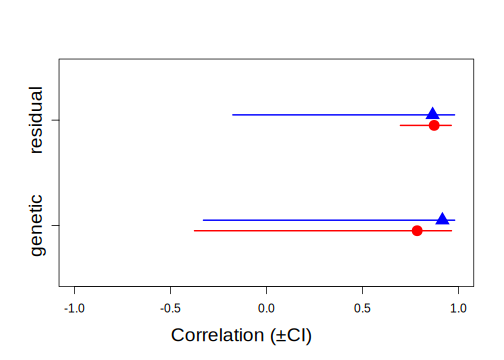
\includegraphics{wam_tuto_files/figure-latex/unnamed-chunk-133-1.pdf}

These posterior distributions overlap between each other, which suggested the correlation were not significantly different between sexes.

By using \texttt{corgh}instead of \texttt{us}, we can extract the BLUPs and plot the sex-specific correlation.

\begin{Shaded}
\begin{Highlighting}[]
\NormalTok{gryphon2}\OperatorTok{$}\NormalTok{T1 \textless{}{-}}\StringTok{ }\NormalTok{gryphon2}\OperatorTok{$}\NormalTok{bwt}
\NormalTok{gryphon2}\OperatorTok{$}\NormalTok{T2 \textless{}{-}}\StringTok{ }\NormalTok{gryphon2}\OperatorTok{$}\NormalTok{tarsus}
\CommentTok{\#}
\NormalTok{model2}\FloatTok{.5}\NormalTok{ \textless{}{-}}\StringTok{ }\KeywordTok{MCMCglmm}\NormalTok{(}\KeywordTok{cbind}\NormalTok{(T1, T2) }\OperatorTok{\textasciitilde{}}\StringTok{ }\NormalTok{trait }\OperatorTok{{-}}\StringTok{ }\DecValTok{1} \OperatorTok{+}\StringTok{ }\NormalTok{trait}\OperatorTok{:}\NormalTok{sex,}
  \DataTypeTok{random =} \OperatorTok{\textasciitilde{}}\StringTok{ }\KeywordTok{corgh}\NormalTok{(}\KeywordTok{at.level}\NormalTok{(sex, }\StringTok{"1"}\NormalTok{)}\OperatorTok{:}\NormalTok{trait)}\OperatorTok{:}\NormalTok{animal }\OperatorTok{+}\StringTok{ }\KeywordTok{corgh}\NormalTok{(}\KeywordTok{at.level}\NormalTok{(sex, }\StringTok{"2"}\NormalTok{)}\OperatorTok{:}\NormalTok{trait)}\OperatorTok{:}\NormalTok{animal }\OperatorTok{+}\StringTok{ }\KeywordTok{idh}\NormalTok{(trait)}\OperatorTok{:}\NormalTok{byear }\OperatorTok{+}\StringTok{ }\KeywordTok{idh}\NormalTok{(trait)}\OperatorTok{:}\NormalTok{mother,}
  \DataTypeTok{rcov =} \OperatorTok{\textasciitilde{}}\StringTok{ }\KeywordTok{us}\NormalTok{(}\KeywordTok{at.level}\NormalTok{(sex, }\StringTok{"1"}\NormalTok{)}\OperatorTok{:}\NormalTok{trait)}\OperatorTok{:}\NormalTok{units }\OperatorTok{+}\StringTok{ }\KeywordTok{us}\NormalTok{(}\KeywordTok{at.level}\NormalTok{(sex, }\StringTok{"2"}\NormalTok{)}\OperatorTok{:}\NormalTok{trait)}\OperatorTok{:}\NormalTok{units,}
  \DataTypeTok{family =} \KeywordTok{c}\NormalTok{(}\StringTok{"gaussian"}\NormalTok{, }\StringTok{"gaussian"}\NormalTok{),}
  \DataTypeTok{ginv =} \KeywordTok{list}\NormalTok{(}\DataTypeTok{animal =}\NormalTok{ Ainv), }\DataTypeTok{data =}\NormalTok{ gryphon2,}
  \DataTypeTok{nitt =} \DecValTok{130000}\NormalTok{, }\DataTypeTok{thin =} \DecValTok{100}\NormalTok{, }\DataTypeTok{burnin =} \DecValTok{30000}\NormalTok{,}
  \DataTypeTok{prior =}\NormalTok{ prior2}\FloatTok{.3}\NormalTok{, }\DataTypeTok{verbose =} \OtherTok{FALSE}\NormalTok{, }\DataTypeTok{pr =} \OtherTok{TRUE}\NormalTok{,}
\NormalTok{)}

\KeywordTok{save}\NormalTok{(model2}\FloatTok{.5}\NormalTok{, }\DataTypeTok{file =} \StringTok{"data/MCMCglmm\_model2\_5\_LongRun.rda"}\NormalTok{)}
\end{Highlighting}
\end{Shaded}

Again we have provided the data from one such run. It can be accessed using the code:

\begin{Shaded}
\begin{Highlighting}[]
\KeywordTok{load}\NormalTok{(}\DataTypeTok{file =} \StringTok{"data/MCMCglmm\_model2\_5\_LongRun.rda"}\NormalTok{)}
\KeywordTok{summary}\NormalTok{(model2}\FloatTok{.5}\NormalTok{)}
\end{Highlighting}
\end{Shaded}

\begin{verbatim}
## 
##  Iterations = 30001:129901
##  Thinning interval  = 100
##  Sample size  = 1000 
## 
##  DIC: 6271.158 
## 
##  G-structure:  ~corgh(at.level(sex, "1"):trait):animal
## 
##                                                              post.mean l-95% CI
## at.level(sex, "1"):traitT1:at.level(sex, "1"):traitT1.animal         1        1
## at.level(sex, "1"):traitT2:at.level(sex, "1"):traitT1.animal         1        1
## at.level(sex, "1"):traitT1:at.level(sex, "1"):traitT2.animal         1        1
## at.level(sex, "1"):traitT2:at.level(sex, "1"):traitT2.animal         1        1
##                                                              u-95% CI eff.samp
## at.level(sex, "1"):traitT1:at.level(sex, "1"):traitT1.animal        1      0.0
## at.level(sex, "1"):traitT2:at.level(sex, "1"):traitT1.animal        1    139.2
## at.level(sex, "1"):traitT1:at.level(sex, "1"):traitT2.animal        1    139.2
## at.level(sex, "1"):traitT2:at.level(sex, "1"):traitT2.animal        1      0.0
## 
##                ~corgh(at.level(sex, "2"):trait):animal
## 
##                                                              post.mean l-95% CI
## at.level(sex, "2"):traitT1:at.level(sex, "2"):traitT1.animal         1        1
## at.level(sex, "2"):traitT2:at.level(sex, "2"):traitT1.animal         1        1
## at.level(sex, "2"):traitT1:at.level(sex, "2"):traitT2.animal         1        1
## at.level(sex, "2"):traitT2:at.level(sex, "2"):traitT2.animal         1        1
##                                                              u-95% CI eff.samp
## at.level(sex, "2"):traitT1:at.level(sex, "2"):traitT1.animal        1      0.0
## at.level(sex, "2"):traitT2:at.level(sex, "2"):traitT1.animal        1    117.2
## at.level(sex, "2"):traitT1:at.level(sex, "2"):traitT2.animal        1    117.2
## at.level(sex, "2"):traitT2:at.level(sex, "2"):traitT2.animal        1      0.0
## 
##                ~idh(trait):byear
## 
##               post.mean l-95% CI u-95% CI eff.samp
## traitT1.byear    0.9381   0.4298    1.542     1309
## traitT2.byear    3.9257   1.7247    6.792     1000
## 
##                ~idh(trait):mother
## 
##                post.mean l-95% CI u-95% CI eff.samp
## traitT1.mother     1.906    1.405    2.353     1000
## traitT2.mother     7.756    5.064   10.104     1000
## 
##  R-structure:  ~us(at.level(sex, "1"):trait):units
## 
##                                                             post.mean l-95% CI
## at.level(sex, "1"):traitT1:at.level(sex, "1"):traitT1.units     2.138    1.538
## at.level(sex, "1"):traitT2:at.level(sex, "1"):traitT1.units     4.599    3.264
## at.level(sex, "1"):traitT1:at.level(sex, "1"):traitT2.units     4.599    3.264
## at.level(sex, "1"):traitT2:at.level(sex, "1"):traitT2.units    15.897   12.695
##                                                             u-95% CI eff.samp
## at.level(sex, "1"):traitT1:at.level(sex, "1"):traitT1.units    2.724     1010
## at.level(sex, "1"):traitT2:at.level(sex, "1"):traitT1.units    5.762     1000
## at.level(sex, "1"):traitT1:at.level(sex, "1"):traitT2.units    5.762     1000
## at.level(sex, "1"):traitT2:at.level(sex, "1"):traitT2.units   19.557     1000
## 
##                ~us(at.level(sex, "2"):trait):units
## 
##                                                             post.mean l-95% CI
## at.level(sex, "2"):traitT1:at.level(sex, "2"):traitT1.units     2.304    1.705
## at.level(sex, "2"):traitT2:at.level(sex, "2"):traitT1.units     5.578    4.305
## at.level(sex, "2"):traitT1:at.level(sex, "2"):traitT2.units     5.578    4.305
## at.level(sex, "2"):traitT2:at.level(sex, "2"):traitT2.units    20.399   16.622
##                                                             u-95% CI eff.samp
## at.level(sex, "2"):traitT1:at.level(sex, "2"):traitT1.units    2.860     1000
## at.level(sex, "2"):traitT2:at.level(sex, "2"):traitT1.units    6.909     1099
## at.level(sex, "2"):traitT1:at.level(sex, "2"):traitT2.units    6.909     1099
## at.level(sex, "2"):traitT2:at.level(sex, "2"):traitT2.units   24.475     1000
## 
##  Location effects: cbind(T1, T2) ~ trait - 1 + trait:sex 
## 
##              post.mean l-95% CI u-95% CI eff.samp  pMCMC    
## traitT1        6.31127  5.82475  6.73755     1138 <0.001 ***
## traitT2       20.51915 19.62675 21.52179     1000 <0.001 ***
## traitT1:sex2   2.01404  1.61651  2.40538     1000 <0.001 ***
## traitT2:sex2   0.07302 -0.73542  0.84480      825  0.862    
## ---
## Signif. codes:  0 '***' 0.001 '**' 0.01 '*' 0.05 '.' 0.1 ' ' 1
\end{verbatim}

\begin{Shaded}
\begin{Highlighting}[]
\KeywordTok{autocorr}\NormalTok{(model2}\FloatTok{.5}\OperatorTok{$}\NormalTok{VCV)}
\end{Highlighting}
\end{Shaded}

\begin{verbatim}
## , , at.level(sex, "1"):traitT1:at.level(sex, "1"):traitT1.animal
## 
##          at.level(sex, "1"):traitT1:at.level(sex, "1"):traitT1.animal
## Lag 0                                                     1.000000000
## Lag 100                                                  -0.001391944
## Lag 500                                                  -0.001397506
## Lag 1000                                                 -0.001404458
## Lag 5000                                                 -0.001983576
##          at.level(sex, "1"):traitT2:at.level(sex, "1"):traitT1.animal
## Lag 0                                                    -0.004648432
## Lag 100                                                  -0.004565467
## Lag 500                                                  -0.005210530
## Lag 1000                                                 -0.011578289
## Lag 5000                                                 -0.005168617
##          at.level(sex, "1"):traitT1:at.level(sex, "1"):traitT2.animal
## Lag 0                                                    -0.004648432
## Lag 100                                                  -0.004565467
## Lag 500                                                  -0.005210530
## Lag 1000                                                 -0.011578289
## Lag 5000                                                 -0.005168617
##          at.level(sex, "1"):traitT2:at.level(sex, "1"):traitT2.animal
## Lag 0                                                     1.000000000
## Lag 100                                                  -0.001391944
## Lag 500                                                  -0.001397506
## Lag 1000                                                 -0.001404458
## Lag 5000                                                 -0.001983576
##          at.level(sex, "2"):traitT1:at.level(sex, "2"):traitT1.animal
## Lag 0                                                   -0.0006350552
## Lag 100                                                 -0.0006356902
## Lag 500                                                 -0.0006382304
## Lag 1000                                                -0.0010042903
## Lag 5000                                                -0.0010296922
##          at.level(sex, "2"):traitT2:at.level(sex, "2"):traitT1.animal
## Lag 0                                                    -0.001456198
## Lag 100                                                  -0.001077247
## Lag 500                                                  -0.002490439
## Lag 1000                                                 -0.005282054
## Lag 5000                                                 -0.006612499
##          at.level(sex, "2"):traitT1:at.level(sex, "2"):traitT2.animal
## Lag 0                                                    -0.001456198
## Lag 100                                                  -0.001077247
## Lag 500                                                  -0.002490439
## Lag 1000                                                 -0.005282054
## Lag 5000                                                 -0.006612499
##          at.level(sex, "2"):traitT2:at.level(sex, "2"):traitT2.animal
## Lag 0                                                   -0.0006350554
## Lag 100                                                 -0.0006356904
## Lag 500                                                 -0.0006382306
## Lag 1000                                                -0.0010042906
## Lag 5000                                                -0.0010296924
##          traitT1.byear traitT2.byear traitT1.mother traitT2.mother
## Lag 0       0.01795130   0.009525697     0.01165057   -0.022459989
## Lag 100    -0.02230357   0.018537495     0.01908830   -0.004395967
## Lag 500     0.01133334   0.034563646     0.02966327   -0.024803073
## Lag 1000    0.02568159  -0.072909756     0.01174105    0.008341327
## Lag 5000   -0.00165152  -0.040694308    -0.01713262   -0.022155338
##          at.level(sex, "1"):traitT1:at.level(sex, "1"):traitT1.units
## Lag 0                                                    0.022762565
## Lag 100                                                  0.013550715
## Lag 500                                                  0.023394975
## Lag 1000                                                 0.003721016
## Lag 5000                                                -0.019698113
##          at.level(sex, "1"):traitT2:at.level(sex, "1"):traitT1.units
## Lag 0                                                    0.022365674
## Lag 100                                                  0.041651846
## Lag 500                                                  0.012710980
## Lag 1000                                                -0.011480840
## Lag 5000                                                -0.001466941
##          at.level(sex, "1"):traitT1:at.level(sex, "1"):traitT2.units
## Lag 0                                                    0.022365674
## Lag 100                                                  0.041651846
## Lag 500                                                  0.012710980
## Lag 1000                                                -0.011480840
## Lag 5000                                                -0.001466941
##          at.level(sex, "1"):traitT2:at.level(sex, "1"):traitT2.units
## Lag 0                                                   -0.010314628
## Lag 100                                                  0.055525653
## Lag 500                                                 -0.003105893
## Lag 1000                                                -0.025454553
## Lag 5000                                                 0.008550330
##          at.level(sex, "2"):traitT1:at.level(sex, "2"):traitT1.units
## Lag 0                                                    0.041893462
## Lag 100                                                 -0.005652676
## Lag 500                                                  0.062306138
## Lag 1000                                                 0.021660306
## Lag 5000                                                -0.009682721
##          at.level(sex, "2"):traitT2:at.level(sex, "2"):traitT1.units
## Lag 0                                                   0.0674542988
## Lag 100                                                -0.0276604979
## Lag 500                                                 0.0278254174
## Lag 1000                                                0.0335689393
## Lag 5000                                                0.0008595584
##          at.level(sex, "2"):traitT1:at.level(sex, "2"):traitT2.units
## Lag 0                                                   0.0674542988
## Lag 100                                                -0.0276604979
## Lag 500                                                 0.0278254174
## Lag 1000                                                0.0335689393
## Lag 5000                                                0.0008595584
##          at.level(sex, "2"):traitT2:at.level(sex, "2"):traitT2.units
## Lag 0                                                    0.081823186
## Lag 100                                                 -0.039860699
## Lag 500                                                  0.008092171
## Lag 1000                                                 0.008412668
## Lag 5000                                                 0.021467565
## 
## , , at.level(sex, "1"):traitT2:at.level(sex, "1"):traitT1.animal
## 
##          at.level(sex, "1"):traitT1:at.level(sex, "1"):traitT1.animal
## Lag 0                                                    -0.004648432
## Lag 100                                                  -0.004625049
## Lag 500                                                  -0.003531126
## Lag 1000                                                 -0.004439099
## Lag 5000                                                 -0.006278871
##          at.level(sex, "1"):traitT2:at.level(sex, "1"):traitT1.animal
## Lag 0                                                     1.000000000
## Lag 100                                                   0.723181023
## Lag 500                                                   0.292398811
## Lag 1000                                                  0.092837234
## Lag 5000                                                 -0.009749071
##          at.level(sex, "1"):traitT1:at.level(sex, "1"):traitT2.animal
## Lag 0                                                     1.000000000
## Lag 100                                                   0.723181023
## Lag 500                                                   0.292398811
## Lag 1000                                                  0.092837234
## Lag 5000                                                 -0.009749071
##          at.level(sex, "1"):traitT2:at.level(sex, "1"):traitT2.animal
## Lag 0                                                    -0.004648437
## Lag 100                                                  -0.004625085
## Lag 500                                                  -0.003531141
## Lag 1000                                                 -0.004439104
## Lag 5000                                                 -0.006278871
##          at.level(sex, "2"):traitT1:at.level(sex, "2"):traitT1.animal
## Lag 0                                                    -0.002312162
## Lag 100                                                  -0.002217551
## Lag 500                                                  -0.001837789
## Lag 1000                                                 -0.002977420
## Lag 5000                                                 -0.004726772
##          at.level(sex, "2"):traitT2:at.level(sex, "2"):traitT1.animal
## Lag 0                                                    -0.010685598
## Lag 100                                                  -0.008503067
## Lag 500                                                  -0.007387620
## Lag 1000                                                 -0.012150586
## Lag 5000                                                 -0.019200093
##          at.level(sex, "2"):traitT1:at.level(sex, "2"):traitT2.animal
## Lag 0                                                    -0.010685598
## Lag 100                                                  -0.008503067
## Lag 500                                                  -0.007387620
## Lag 1000                                                 -0.012150586
## Lag 5000                                                 -0.019200093
##          at.level(sex, "2"):traitT2:at.level(sex, "2"):traitT2.animal
## Lag 0                                                    -0.002312162
## Lag 100                                                  -0.002217551
## Lag 500                                                  -0.001837789
## Lag 1000                                                 -0.002977420
## Lag 5000                                                 -0.004726772
##          traitT1.byear traitT2.byear traitT1.mother traitT2.mother
## Lag 0       0.03206603   0.001388092    -0.01597305   -0.012121778
## Lag 100     0.02062954  -0.034683825     0.01430611   -0.050389774
## Lag 500     0.01419036   0.020814008     0.03068981   -0.018472864
## Lag 1000    0.02272278  -0.003124614    -0.03666507    0.008391569
## Lag 5000   -0.01889532  -0.003299003    -0.03161363    0.042393770
##          at.level(sex, "1"):traitT1:at.level(sex, "1"):traitT1.units
## Lag 0                                                   -0.022308219
## Lag 100                                                 -0.004067301
## Lag 500                                                 -0.004473470
## Lag 1000                                                 0.048582961
## Lag 5000                                                 0.001202075
##          at.level(sex, "1"):traitT2:at.level(sex, "1"):traitT1.units
## Lag 0                                                   -0.015759766
## Lag 100                                                  0.017032779
## Lag 500                                                 -0.003108186
## Lag 1000                                                 0.042126244
## Lag 5000                                                -0.016955230
##          at.level(sex, "1"):traitT1:at.level(sex, "1"):traitT2.units
## Lag 0                                                   -0.015759766
## Lag 100                                                  0.017032779
## Lag 500                                                 -0.003108186
## Lag 1000                                                 0.042126244
## Lag 5000                                                -0.016955230
##          at.level(sex, "1"):traitT2:at.level(sex, "1"):traitT2.units
## Lag 0                                                   -0.008530358
## Lag 100                                                  0.019755361
## Lag 500                                                 -0.013140805
## Lag 1000                                                 0.013898534
## Lag 5000                                                -0.033469898
##          at.level(sex, "2"):traitT1:at.level(sex, "2"):traitT1.units
## Lag 0                                                    0.005815507
## Lag 100                                                  0.001279903
## Lag 500                                                 -0.004227436
## Lag 1000                                                -0.037409946
## Lag 5000                                                 0.027223985
##          at.level(sex, "2"):traitT2:at.level(sex, "2"):traitT1.units
## Lag 0                                                   -0.028111911
## Lag 100                                                 -0.015823870
## Lag 500                                                 -0.002146573
## Lag 1000                                                -0.016376141
## Lag 5000                                                 0.038876537
##          at.level(sex, "2"):traitT1:at.level(sex, "2"):traitT2.units
## Lag 0                                                   -0.028111911
## Lag 100                                                 -0.015823870
## Lag 500                                                 -0.002146573
## Lag 1000                                                -0.016376141
## Lag 5000                                                 0.038876537
##          at.level(sex, "2"):traitT2:at.level(sex, "2"):traitT2.units
## Lag 0                                                   -0.042456056
## Lag 100                                                 -0.010621969
## Lag 500                                                  0.009797485
## Lag 1000                                                -0.019305202
## Lag 5000                                                 0.033404201
## 
## , , at.level(sex, "1"):traitT1:at.level(sex, "1"):traitT2.animal
## 
##          at.level(sex, "1"):traitT1:at.level(sex, "1"):traitT1.animal
## Lag 0                                                    -0.004648432
## Lag 100                                                  -0.004625049
## Lag 500                                                  -0.003531126
## Lag 1000                                                 -0.004439099
## Lag 5000                                                 -0.006278871
##          at.level(sex, "1"):traitT2:at.level(sex, "1"):traitT1.animal
## Lag 0                                                     1.000000000
## Lag 100                                                   0.723181023
## Lag 500                                                   0.292398811
## Lag 1000                                                  0.092837234
## Lag 5000                                                 -0.009749071
##          at.level(sex, "1"):traitT1:at.level(sex, "1"):traitT2.animal
## Lag 0                                                     1.000000000
## Lag 100                                                   0.723181023
## Lag 500                                                   0.292398811
## Lag 1000                                                  0.092837234
## Lag 5000                                                 -0.009749071
##          at.level(sex, "1"):traitT2:at.level(sex, "1"):traitT2.animal
## Lag 0                                                    -0.004648437
## Lag 100                                                  -0.004625085
## Lag 500                                                  -0.003531141
## Lag 1000                                                 -0.004439104
## Lag 5000                                                 -0.006278871
##          at.level(sex, "2"):traitT1:at.level(sex, "2"):traitT1.animal
## Lag 0                                                    -0.002312162
## Lag 100                                                  -0.002217551
## Lag 500                                                  -0.001837789
## Lag 1000                                                 -0.002977420
## Lag 5000                                                 -0.004726772
##          at.level(sex, "2"):traitT2:at.level(sex, "2"):traitT1.animal
## Lag 0                                                    -0.010685598
## Lag 100                                                  -0.008503067
## Lag 500                                                  -0.007387620
## Lag 1000                                                 -0.012150586
## Lag 5000                                                 -0.019200093
##          at.level(sex, "2"):traitT1:at.level(sex, "2"):traitT2.animal
## Lag 0                                                    -0.010685598
## Lag 100                                                  -0.008503067
## Lag 500                                                  -0.007387620
## Lag 1000                                                 -0.012150586
## Lag 5000                                                 -0.019200093
##          at.level(sex, "2"):traitT2:at.level(sex, "2"):traitT2.animal
## Lag 0                                                    -0.002312162
## Lag 100                                                  -0.002217551
## Lag 500                                                  -0.001837789
## Lag 1000                                                 -0.002977420
## Lag 5000                                                 -0.004726772
##          traitT1.byear traitT2.byear traitT1.mother traitT2.mother
## Lag 0       0.03206603   0.001388092    -0.01597305   -0.012121778
## Lag 100     0.02062954  -0.034683825     0.01430611   -0.050389774
## Lag 500     0.01419036   0.020814008     0.03068981   -0.018472864
## Lag 1000    0.02272278  -0.003124614    -0.03666507    0.008391569
## Lag 5000   -0.01889532  -0.003299003    -0.03161363    0.042393770
##          at.level(sex, "1"):traitT1:at.level(sex, "1"):traitT1.units
## Lag 0                                                   -0.022308219
## Lag 100                                                 -0.004067301
## Lag 500                                                 -0.004473470
## Lag 1000                                                 0.048582961
## Lag 5000                                                 0.001202075
##          at.level(sex, "1"):traitT2:at.level(sex, "1"):traitT1.units
## Lag 0                                                   -0.015759766
## Lag 100                                                  0.017032779
## Lag 500                                                 -0.003108186
## Lag 1000                                                 0.042126244
## Lag 5000                                                -0.016955230
##          at.level(sex, "1"):traitT1:at.level(sex, "1"):traitT2.units
## Lag 0                                                   -0.015759766
## Lag 100                                                  0.017032779
## Lag 500                                                 -0.003108186
## Lag 1000                                                 0.042126244
## Lag 5000                                                -0.016955230
##          at.level(sex, "1"):traitT2:at.level(sex, "1"):traitT2.units
## Lag 0                                                   -0.008530358
## Lag 100                                                  0.019755361
## Lag 500                                                 -0.013140805
## Lag 1000                                                 0.013898534
## Lag 5000                                                -0.033469898
##          at.level(sex, "2"):traitT1:at.level(sex, "2"):traitT1.units
## Lag 0                                                    0.005815507
## Lag 100                                                  0.001279903
## Lag 500                                                 -0.004227436
## Lag 1000                                                -0.037409946
## Lag 5000                                                 0.027223985
##          at.level(sex, "2"):traitT2:at.level(sex, "2"):traitT1.units
## Lag 0                                                   -0.028111911
## Lag 100                                                 -0.015823870
## Lag 500                                                 -0.002146573
## Lag 1000                                                -0.016376141
## Lag 5000                                                 0.038876537
##          at.level(sex, "2"):traitT1:at.level(sex, "2"):traitT2.units
## Lag 0                                                   -0.028111911
## Lag 100                                                 -0.015823870
## Lag 500                                                 -0.002146573
## Lag 1000                                                -0.016376141
## Lag 5000                                                 0.038876537
##          at.level(sex, "2"):traitT2:at.level(sex, "2"):traitT2.units
## Lag 0                                                   -0.042456056
## Lag 100                                                 -0.010621969
## Lag 500                                                  0.009797485
## Lag 1000                                                -0.019305202
## Lag 5000                                                 0.033404201
## 
## , , at.level(sex, "1"):traitT2:at.level(sex, "1"):traitT2.animal
## 
##          at.level(sex, "1"):traitT1:at.level(sex, "1"):traitT1.animal
## Lag 0                                                     1.000000000
## Lag 100                                                  -0.001391944
## Lag 500                                                  -0.001397506
## Lag 1000                                                 -0.001404458
## Lag 5000                                                 -0.001983576
##          at.level(sex, "1"):traitT2:at.level(sex, "1"):traitT1.animal
## Lag 0                                                    -0.004648437
## Lag 100                                                  -0.004565469
## Lag 500                                                  -0.005210530
## Lag 1000                                                 -0.011578289
## Lag 5000                                                 -0.005168617
##          at.level(sex, "1"):traitT1:at.level(sex, "1"):traitT2.animal
## Lag 0                                                    -0.004648437
## Lag 100                                                  -0.004565469
## Lag 500                                                  -0.005210530
## Lag 1000                                                 -0.011578289
## Lag 5000                                                 -0.005168617
##          at.level(sex, "1"):traitT2:at.level(sex, "1"):traitT2.animal
## Lag 0                                                     1.000000000
## Lag 100                                                  -0.001391944
## Lag 500                                                  -0.001397506
## Lag 1000                                                 -0.001404458
## Lag 5000                                                 -0.001983576
##          at.level(sex, "2"):traitT1:at.level(sex, "2"):traitT1.animal
## Lag 0                                                   -0.0006350551
## Lag 100                                                 -0.0006356902
## Lag 500                                                 -0.0006382304
## Lag 1000                                                -0.0010042903
## Lag 5000                                                -0.0010296921
##          at.level(sex, "2"):traitT2:at.level(sex, "2"):traitT1.animal
## Lag 0                                                    -0.001456198
## Lag 100                                                  -0.001077247
## Lag 500                                                  -0.002490439
## Lag 1000                                                 -0.005282054
## Lag 5000                                                 -0.006612499
##          at.level(sex, "2"):traitT1:at.level(sex, "2"):traitT2.animal
## Lag 0                                                    -0.001456198
## Lag 100                                                  -0.001077247
## Lag 500                                                  -0.002490439
## Lag 1000                                                 -0.005282054
## Lag 5000                                                 -0.006612499
##          at.level(sex, "2"):traitT2:at.level(sex, "2"):traitT2.animal
## Lag 0                                                   -0.0006350554
## Lag 100                                                 -0.0006356904
## Lag 500                                                 -0.0006382306
## Lag 1000                                                -0.0010042906
## Lag 5000                                                -0.0010296924
##          traitT1.byear traitT2.byear traitT1.mother traitT2.mother
## Lag 0      0.017951297   0.009525703     0.01165057   -0.022459984
## Lag 100   -0.022303567   0.018537496     0.01908830   -0.004395967
## Lag 500    0.011333343   0.034563646     0.02966327   -0.024803074
## Lag 1000   0.025681592  -0.072909754     0.01174105    0.008341327
## Lag 5000  -0.001651524  -0.040694308    -0.01713262   -0.022155336
##          at.level(sex, "1"):traitT1:at.level(sex, "1"):traitT1.units
## Lag 0                                                    0.022762562
## Lag 100                                                  0.013550715
## Lag 500                                                  0.023394973
## Lag 1000                                                 0.003721019
## Lag 5000                                                -0.019698116
##          at.level(sex, "1"):traitT2:at.level(sex, "1"):traitT1.units
## Lag 0                                                    0.022365669
## Lag 100                                                  0.041651846
## Lag 500                                                  0.012710977
## Lag 1000                                                -0.011480840
## Lag 5000                                                -0.001466943
##          at.level(sex, "1"):traitT1:at.level(sex, "1"):traitT2.units
## Lag 0                                                    0.022365669
## Lag 100                                                  0.041651846
## Lag 500                                                  0.012710977
## Lag 1000                                                -0.011480840
## Lag 5000                                                -0.001466943
##          at.level(sex, "1"):traitT2:at.level(sex, "1"):traitT2.units
## Lag 0                                                   -0.010314633
## Lag 100                                                  0.055525653
## Lag 500                                                 -0.003105895
## Lag 1000                                                -0.025454554
## Lag 5000                                                 0.008550329
##          at.level(sex, "2"):traitT1:at.level(sex, "2"):traitT1.units
## Lag 0                                                    0.041893463
## Lag 100                                                 -0.005652675
## Lag 500                                                  0.062306141
## Lag 1000                                                 0.021660305
## Lag 5000                                                -0.009682725
##          at.level(sex, "2"):traitT2:at.level(sex, "2"):traitT1.units
## Lag 0                                                   0.0674542971
## Lag 100                                                -0.0276604962
## Lag 500                                                 0.0278254213
## Lag 1000                                                0.0335689362
## Lag 5000                                                0.0008595534
##          at.level(sex, "2"):traitT1:at.level(sex, "2"):traitT2.units
## Lag 0                                                   0.0674542971
## Lag 100                                                -0.0276604962
## Lag 500                                                 0.0278254213
## Lag 1000                                                0.0335689362
## Lag 5000                                                0.0008595534
##          at.level(sex, "2"):traitT2:at.level(sex, "2"):traitT2.units
## Lag 0                                                    0.081823182
## Lag 100                                                 -0.039860695
## Lag 500                                                  0.008092176
## Lag 1000                                                 0.008412663
## Lag 5000                                                 0.021467560
## 
## , , at.level(sex, "2"):traitT1:at.level(sex, "2"):traitT1.animal
## 
##          at.level(sex, "1"):traitT1:at.level(sex, "1"):traitT1.animal
## Lag 0                                                   -0.0006350552
## Lag 100                                                 -0.0002728055
## Lag 500                                                 -0.0002753457
## Lag 1000                                                -0.0002785209
## Lag 5000                                                -0.0005430012
##          at.level(sex, "1"):traitT2:at.level(sex, "1"):traitT1.animal
## Lag 0                                                   -0.0023121624
## Lag 100                                                 -0.0018131603
## Lag 500                                                 -0.0021171712
## Lag 1000                                                -0.0002636656
## Lag 5000                                                -0.0007281379
##          at.level(sex, "1"):traitT1:at.level(sex, "1"):traitT2.animal
## Lag 0                                                   -0.0023121624
## Lag 100                                                 -0.0018131603
## Lag 500                                                 -0.0021171712
## Lag 1000                                                -0.0002636656
## Lag 5000                                                -0.0007281379
##          at.level(sex, "1"):traitT2:at.level(sex, "1"):traitT2.animal
## Lag 0                                                   -0.0006350551
## Lag 100                                                 -0.0002728055
## Lag 500                                                 -0.0002753457
## Lag 1000                                                -0.0002785209
## Lag 5000                                                -0.0005430012
##          at.level(sex, "2"):traitT1:at.level(sex, "2"):traitT1.animal
## Lag 0                                                    1.0000000000
## Lag 100                                                 -0.0001245872
## Lag 500                                                  0.0472252652
## Lag 1000                                                -0.0002929252
## Lag 5000                                                -0.0003045261
##          at.level(sex, "2"):traitT2:at.level(sex, "2"):traitT1.animal
## Lag 0                                                   -0.0030464876
## Lag 100                                                 -0.0012272569
## Lag 500                                                 -0.0012428417
## Lag 1000                                                -0.0009101059
## Lag 5000                                                -0.0098179074
##          at.level(sex, "2"):traitT1:at.level(sex, "2"):traitT2.animal
## Lag 0                                                   -0.0030464876
## Lag 100                                                 -0.0012272569
## Lag 500                                                 -0.0012428417
## Lag 1000                                                -0.0009101059
## Lag 5000                                                -0.0098179074
##          at.level(sex, "2"):traitT2:at.level(sex, "2"):traitT2.animal
## Lag 0                                                    1.0000000000
## Lag 100                                                 -0.0001245873
## Lag 500                                                  0.0472252675
## Lag 1000                                                -0.0002929253
## Lag 5000                                                -0.0003045262
##          traitT1.byear traitT2.byear traitT1.mother traitT2.mother
## Lag 0      0.007859897  -0.048647022    0.014169960    -0.01277587
## Lag 100   -0.031686328   0.044252052    0.001418991    -0.00470343
## Lag 500   -0.006041444  -0.003672647    0.026635103    -0.05216309
## Lag 1000   0.040389650   0.001576320   -0.008599945    -0.03098371
## Lag 5000  -0.014128580  -0.030023647    0.016865943    -0.08562409
##          at.level(sex, "1"):traitT1:at.level(sex, "1"):traitT1.units
## Lag 0                                                    0.019317584
## Lag 100                                                 -0.006883423
## Lag 500                                                  0.005456272
## Lag 1000                                                -0.040428229
## Lag 5000                                                -0.019377516
##          at.level(sex, "1"):traitT2:at.level(sex, "1"):traitT1.units
## Lag 0                                                    0.002652222
## Lag 100                                                 -0.016499071
## Lag 500                                                 -0.004463759
## Lag 1000                                                -0.044909299
## Lag 5000                                                -0.009389202
##          at.level(sex, "1"):traitT1:at.level(sex, "1"):traitT2.units
## Lag 0                                                    0.002652222
## Lag 100                                                 -0.016499071
## Lag 500                                                 -0.004463759
## Lag 1000                                                -0.044909299
## Lag 5000                                                -0.009389202
##          at.level(sex, "1"):traitT2:at.level(sex, "1"):traitT2.units
## Lag 0                                                   -0.002054456
## Lag 100                                                  0.002237526
## Lag 500                                                  0.013746887
## Lag 1000                                                -0.048289160
## Lag 5000                                                 0.014216318
##          at.level(sex, "2"):traitT1:at.level(sex, "2"):traitT1.units
## Lag 0                                                    -0.01258769
## Lag 100                                                   0.01872011
## Lag 500                                                   0.01882522
## Lag 1000                                                  0.03756773
## Lag 5000                                                 -0.02411450
##          at.level(sex, "2"):traitT2:at.level(sex, "2"):traitT1.units
## Lag 0                                                   -0.005906983
## Lag 100                                                  0.013146223
## Lag 500                                                  0.043916861
## Lag 1000                                                 0.033507898
## Lag 5000                                                -0.008078930
##          at.level(sex, "2"):traitT1:at.level(sex, "2"):traitT2.units
## Lag 0                                                   -0.005906983
## Lag 100                                                  0.013146223
## Lag 500                                                  0.043916861
## Lag 1000                                                 0.033507898
## Lag 5000                                                -0.008078930
##          at.level(sex, "2"):traitT2:at.level(sex, "2"):traitT2.units
## Lag 0                                                   0.0006335032
## Lag 100                                                 0.0037825580
## Lag 500                                                 0.0543707513
## Lag 1000                                                0.0360053763
## Lag 5000                                               -0.0061125594
## 
## , , at.level(sex, "2"):traitT2:at.level(sex, "2"):traitT1.animal
## 
##          at.level(sex, "1"):traitT1:at.level(sex, "1"):traitT1.animal
## Lag 0                                                    -0.001456198
## Lag 100                                                   0.001715826
## Lag 500                                                  -0.003740235
## Lag 1000                                                 -0.005014592
## Lag 5000                                                 -0.010487126
##          at.level(sex, "1"):traitT2:at.level(sex, "1"):traitT1.animal
## Lag 0                                                     -0.01068560
## Lag 100                                                   -0.01235479
## Lag 500                                                   -0.01399016
## Lag 1000                                                  -0.01676244
## Lag 5000                                                  -0.01431417
##          at.level(sex, "1"):traitT1:at.level(sex, "1"):traitT2.animal
## Lag 0                                                     -0.01068560
## Lag 100                                                   -0.01235479
## Lag 500                                                   -0.01399016
## Lag 1000                                                  -0.01676244
## Lag 5000                                                  -0.01431417
##          at.level(sex, "1"):traitT2:at.level(sex, "1"):traitT2.animal
## Lag 0                                                    -0.001456198
## Lag 100                                                   0.001715826
## Lag 500                                                  -0.003740235
## Lag 1000                                                 -0.005014592
## Lag 5000                                                 -0.010487126
##          at.level(sex, "2"):traitT1:at.level(sex, "2"):traitT1.animal
## Lag 0                                                    -0.003046488
## Lag 100                                                  -0.003153963
## Lag 500                                                  -0.002352225
## Lag 1000                                                 -0.003782156
## Lag 5000                                                 -0.002857518
##          at.level(sex, "2"):traitT2:at.level(sex, "2"):traitT1.animal
## Lag 0                                                      1.00000000
## Lag 100                                                    0.83058654
## Lag 500                                                    0.23387736
## Lag 1000                                                   0.12487172
## Lag 5000                                                  -0.02765118
##          at.level(sex, "2"):traitT1:at.level(sex, "2"):traitT2.animal
## Lag 0                                                      1.00000000
## Lag 100                                                    0.83058654
## Lag 500                                                    0.23387736
## Lag 1000                                                   0.12487172
## Lag 5000                                                  -0.02765118
##          at.level(sex, "2"):traitT2:at.level(sex, "2"):traitT2.animal
## Lag 0                                                    -0.003046486
## Lag 100                                                  -0.003153962
## Lag 500                                                  -0.002352224
## Lag 1000                                                 -0.003782157
## Lag 5000                                                 -0.002857519
##          traitT1.byear traitT2.byear traitT1.mother traitT2.mother
## Lag 0     -0.013526377   -0.01774985   -0.013841217    0.022701877
## Lag 100    0.004093624   -0.01386591    0.001219680    0.015022006
## Lag 500    0.021634587    0.01429551   -0.019234622    0.022081044
## Lag 1000  -0.020668120    0.05928732   -0.059492408    0.033606722
## Lag 5000  -0.009719164    0.04539140   -0.005427111   -0.008612086
##          at.level(sex, "1"):traitT1:at.level(sex, "1"):traitT1.units
## Lag 0                                                   -0.024077943
## Lag 100                                                 -0.002203887
## Lag 500                                                  0.010909995
## Lag 1000                                                 0.018505117
## Lag 5000                                                -0.065135988
##          at.level(sex, "1"):traitT2:at.level(sex, "1"):traitT1.units
## Lag 0                                                  -0.0072931648
## Lag 100                                                 0.0003911575
## Lag 500                                                 0.0164572902
## Lag 1000                                                0.0161183049
## Lag 5000                                               -0.0518609896
##          at.level(sex, "1"):traitT1:at.level(sex, "1"):traitT2.units
## Lag 0                                                  -0.0072931648
## Lag 100                                                 0.0003911575
## Lag 500                                                 0.0164572902
## Lag 1000                                                0.0161183049
## Lag 5000                                               -0.0518609896
##          at.level(sex, "1"):traitT2:at.level(sex, "1"):traitT2.units
## Lag 0                                                    0.002102035
## Lag 100                                                  0.002516452
## Lag 500                                                  0.016614009
## Lag 1000                                                 0.009102492
## Lag 5000                                                -0.057713146
##          at.level(sex, "2"):traitT1:at.level(sex, "2"):traitT1.units
## Lag 0                                                    0.003830731
## Lag 100                                                 -0.005606418
## Lag 500                                                  0.005332862
## Lag 1000                                                 0.009183940
## Lag 5000                                                -0.021145579
##          at.level(sex, "2"):traitT2:at.level(sex, "2"):traitT1.units
## Lag 0                                                    0.001171218
## Lag 100                                                 -0.012536100
## Lag 500                                                  0.002347666
## Lag 1000                                                 0.012765703
## Lag 5000                                                -0.035720789
##          at.level(sex, "2"):traitT1:at.level(sex, "2"):traitT2.units
## Lag 0                                                    0.001171218
## Lag 100                                                 -0.012536100
## Lag 500                                                  0.002347666
## Lag 1000                                                 0.012765703
## Lag 5000                                                -0.035720789
##          at.level(sex, "2"):traitT2:at.level(sex, "2"):traitT2.units
## Lag 0                                                    0.011573448
## Lag 100                                                  0.010597731
## Lag 500                                                  0.009234753
## Lag 1000                                                 0.017510534
## Lag 5000                                                -0.019205136
## 
## , , at.level(sex, "2"):traitT1:at.level(sex, "2"):traitT2.animal
## 
##          at.level(sex, "1"):traitT1:at.level(sex, "1"):traitT1.animal
## Lag 0                                                    -0.001456198
## Lag 100                                                   0.001715826
## Lag 500                                                  -0.003740235
## Lag 1000                                                 -0.005014592
## Lag 5000                                                 -0.010487126
##          at.level(sex, "1"):traitT2:at.level(sex, "1"):traitT1.animal
## Lag 0                                                     -0.01068560
## Lag 100                                                   -0.01235479
## Lag 500                                                   -0.01399016
## Lag 1000                                                  -0.01676244
## Lag 5000                                                  -0.01431417
##          at.level(sex, "1"):traitT1:at.level(sex, "1"):traitT2.animal
## Lag 0                                                     -0.01068560
## Lag 100                                                   -0.01235479
## Lag 500                                                   -0.01399016
## Lag 1000                                                  -0.01676244
## Lag 5000                                                  -0.01431417
##          at.level(sex, "1"):traitT2:at.level(sex, "1"):traitT2.animal
## Lag 0                                                    -0.001456198
## Lag 100                                                   0.001715826
## Lag 500                                                  -0.003740235
## Lag 1000                                                 -0.005014592
## Lag 5000                                                 -0.010487126
##          at.level(sex, "2"):traitT1:at.level(sex, "2"):traitT1.animal
## Lag 0                                                    -0.003046488
## Lag 100                                                  -0.003153963
## Lag 500                                                  -0.002352225
## Lag 1000                                                 -0.003782156
## Lag 5000                                                 -0.002857518
##          at.level(sex, "2"):traitT2:at.level(sex, "2"):traitT1.animal
## Lag 0                                                      1.00000000
## Lag 100                                                    0.83058654
## Lag 500                                                    0.23387736
## Lag 1000                                                   0.12487172
## Lag 5000                                                  -0.02765118
##          at.level(sex, "2"):traitT1:at.level(sex, "2"):traitT2.animal
## Lag 0                                                      1.00000000
## Lag 100                                                    0.83058654
## Lag 500                                                    0.23387736
## Lag 1000                                                   0.12487172
## Lag 5000                                                  -0.02765118
##          at.level(sex, "2"):traitT2:at.level(sex, "2"):traitT2.animal
## Lag 0                                                    -0.003046486
## Lag 100                                                  -0.003153962
## Lag 500                                                  -0.002352224
## Lag 1000                                                 -0.003782157
## Lag 5000                                                 -0.002857519
##          traitT1.byear traitT2.byear traitT1.mother traitT2.mother
## Lag 0     -0.013526377   -0.01774985   -0.013841217    0.022701877
## Lag 100    0.004093624   -0.01386591    0.001219680    0.015022006
## Lag 500    0.021634587    0.01429551   -0.019234622    0.022081044
## Lag 1000  -0.020668120    0.05928732   -0.059492408    0.033606722
## Lag 5000  -0.009719164    0.04539140   -0.005427111   -0.008612086
##          at.level(sex, "1"):traitT1:at.level(sex, "1"):traitT1.units
## Lag 0                                                   -0.024077943
## Lag 100                                                 -0.002203887
## Lag 500                                                  0.010909995
## Lag 1000                                                 0.018505117
## Lag 5000                                                -0.065135988
##          at.level(sex, "1"):traitT2:at.level(sex, "1"):traitT1.units
## Lag 0                                                  -0.0072931648
## Lag 100                                                 0.0003911575
## Lag 500                                                 0.0164572902
## Lag 1000                                                0.0161183049
## Lag 5000                                               -0.0518609896
##          at.level(sex, "1"):traitT1:at.level(sex, "1"):traitT2.units
## Lag 0                                                  -0.0072931648
## Lag 100                                                 0.0003911575
## Lag 500                                                 0.0164572902
## Lag 1000                                                0.0161183049
## Lag 5000                                               -0.0518609896
##          at.level(sex, "1"):traitT2:at.level(sex, "1"):traitT2.units
## Lag 0                                                    0.002102035
## Lag 100                                                  0.002516452
## Lag 500                                                  0.016614009
## Lag 1000                                                 0.009102492
## Lag 5000                                                -0.057713146
##          at.level(sex, "2"):traitT1:at.level(sex, "2"):traitT1.units
## Lag 0                                                    0.003830731
## Lag 100                                                 -0.005606418
## Lag 500                                                  0.005332862
## Lag 1000                                                 0.009183940
## Lag 5000                                                -0.021145579
##          at.level(sex, "2"):traitT2:at.level(sex, "2"):traitT1.units
## Lag 0                                                    0.001171218
## Lag 100                                                 -0.012536100
## Lag 500                                                  0.002347666
## Lag 1000                                                 0.012765703
## Lag 5000                                                -0.035720789
##          at.level(sex, "2"):traitT1:at.level(sex, "2"):traitT2.units
## Lag 0                                                    0.001171218
## Lag 100                                                 -0.012536100
## Lag 500                                                  0.002347666
## Lag 1000                                                 0.012765703
## Lag 5000                                                -0.035720789
##          at.level(sex, "2"):traitT2:at.level(sex, "2"):traitT2.units
## Lag 0                                                    0.011573448
## Lag 100                                                  0.010597731
## Lag 500                                                  0.009234753
## Lag 1000                                                 0.017510534
## Lag 5000                                                -0.019205136
## 
## , , at.level(sex, "2"):traitT2:at.level(sex, "2"):traitT2.animal
## 
##          at.level(sex, "1"):traitT1:at.level(sex, "1"):traitT1.animal
## Lag 0                                                   -0.0006350554
## Lag 100                                                 -0.0002727894
## Lag 500                                                 -0.0002753459
## Lag 1000                                                -0.0002785211
## Lag 5000                                                -0.0005430015
##          at.level(sex, "1"):traitT2:at.level(sex, "1"):traitT1.animal
## Lag 0                                                   -0.0023121624
## Lag 100                                                 -0.0018131609
## Lag 500                                                 -0.0021171719
## Lag 1000                                                -0.0002636663
## Lag 5000                                                -0.0007281383
##          at.level(sex, "1"):traitT1:at.level(sex, "1"):traitT2.animal
## Lag 0                                                   -0.0023121624
## Lag 100                                                 -0.0018131609
## Lag 500                                                 -0.0021171719
## Lag 1000                                                -0.0002636663
## Lag 5000                                                -0.0007281383
##          at.level(sex, "1"):traitT2:at.level(sex, "1"):traitT2.animal
## Lag 0                                                   -0.0006350554
## Lag 100                                                 -0.0002727894
## Lag 500                                                 -0.0002753459
## Lag 1000                                                -0.0002785211
## Lag 5000                                                -0.0005430015
##          at.level(sex, "2"):traitT1:at.level(sex, "2"):traitT1.animal
## Lag 0                                                    1.0000000000
## Lag 100                                                 -0.0001245873
## Lag 500                                                  0.0472252591
## Lag 1000                                                -0.0002929253
## Lag 5000                                                -0.0003045262
##          at.level(sex, "2"):traitT2:at.level(sex, "2"):traitT1.animal
## Lag 0                                                   -0.0030464862
## Lag 100                                                 -0.0012272567
## Lag 500                                                 -0.0012428427
## Lag 1000                                                -0.0009101069
## Lag 5000                                                -0.0098178961
##          at.level(sex, "2"):traitT1:at.level(sex, "2"):traitT2.animal
## Lag 0                                                   -0.0030464862
## Lag 100                                                 -0.0012272567
## Lag 500                                                 -0.0012428427
## Lag 1000                                                -0.0009101069
## Lag 5000                                                -0.0098178961
##          at.level(sex, "2"):traitT2:at.level(sex, "2"):traitT2.animal
## Lag 0                                                    1.0000000000
## Lag 100                                                 -0.0001245874
## Lag 500                                                  0.0472252614
## Lag 1000                                                -0.0002929254
## Lag 5000                                                -0.0003045263
##          traitT1.byear traitT2.byear traitT1.mother traitT2.mother
## Lag 0      0.007859899  -0.048647026    0.014169961   -0.012775870
## Lag 100   -0.031686329   0.044252052    0.001418992   -0.004703428
## Lag 500   -0.006041443  -0.003672647    0.026635104   -0.052163087
## Lag 1000   0.040389655   0.001576326   -0.008599948   -0.030983703
## Lag 5000  -0.014128581  -0.030023647    0.016865937   -0.085624096
##          at.level(sex, "1"):traitT1:at.level(sex, "1"):traitT1.units
## Lag 0                                                    0.019317585
## Lag 100                                                 -0.006883421
## Lag 500                                                  0.005456271
## Lag 1000                                                -0.040428232
## Lag 5000                                                -0.019377514
##          at.level(sex, "1"):traitT2:at.level(sex, "1"):traitT1.units
## Lag 0                                                    0.002652225
## Lag 100                                                 -0.016499068
## Lag 500                                                 -0.004463759
## Lag 1000                                                -0.044909300
## Lag 5000                                                -0.009389200
##          at.level(sex, "1"):traitT1:at.level(sex, "1"):traitT2.units
## Lag 0                                                    0.002652225
## Lag 100                                                 -0.016499068
## Lag 500                                                 -0.004463759
## Lag 1000                                                -0.044909300
## Lag 5000                                                -0.009389200
##          at.level(sex, "1"):traitT2:at.level(sex, "1"):traitT2.units
## Lag 0                                                   -0.002054453
## Lag 100                                                  0.002237526
## Lag 500                                                  0.013746888
## Lag 1000                                                -0.048289160
## Lag 5000                                                 0.014216318
##          at.level(sex, "2"):traitT1:at.level(sex, "2"):traitT1.units
## Lag 0                                                    -0.01258769
## Lag 100                                                   0.01872011
## Lag 500                                                   0.01882522
## Lag 1000                                                  0.03756772
## Lag 5000                                                 -0.02411450
##          at.level(sex, "2"):traitT2:at.level(sex, "2"):traitT1.units
## Lag 0                                                   -0.005906985
## Lag 100                                                  0.013146221
## Lag 500                                                  0.043916862
## Lag 1000                                                 0.033507897
## Lag 5000                                                -0.008078924
##          at.level(sex, "2"):traitT1:at.level(sex, "2"):traitT2.units
## Lag 0                                                   -0.005906985
## Lag 100                                                  0.013146221
## Lag 500                                                  0.043916862
## Lag 1000                                                 0.033507897
## Lag 5000                                                -0.008078924
##          at.level(sex, "2"):traitT2:at.level(sex, "2"):traitT2.units
## Lag 0                                                   0.0006335012
## Lag 100                                                 0.0037825564
## Lag 500                                                 0.0543707522
## Lag 1000                                                0.0360053770
## Lag 5000                                               -0.0061125543
## 
## , , traitT1.byear
## 
##          at.level(sex, "1"):traitT1:at.level(sex, "1"):traitT1.animal
## Lag 0                                                     0.017951297
## Lag 100                                                  -0.015650603
## Lag 500                                                  -0.048310004
## Lag 1000                                                  0.006748945
## Lag 5000                                                 -0.024695487
##          at.level(sex, "1"):traitT2:at.level(sex, "1"):traitT1.animal
## Lag 0                                                      0.03206603
## Lag 100                                                    0.03644816
## Lag 500                                                    0.02462867
## Lag 1000                                                   0.03134031
## Lag 5000                                                  -0.02813186
##          at.level(sex, "1"):traitT1:at.level(sex, "1"):traitT2.animal
## Lag 0                                                      0.03206603
## Lag 100                                                    0.03644816
## Lag 500                                                    0.02462867
## Lag 1000                                                   0.03134031
## Lag 5000                                                  -0.02813186
##          at.level(sex, "1"):traitT2:at.level(sex, "1"):traitT2.animal
## Lag 0                                                     0.017951297
## Lag 100                                                  -0.015650603
## Lag 500                                                  -0.048310005
## Lag 1000                                                  0.006748946
## Lag 5000                                                 -0.024695489
##          at.level(sex, "2"):traitT1:at.level(sex, "2"):traitT1.animal
## Lag 0                                                     0.007859897
## Lag 100                                                   0.008951424
## Lag 500                                                  -0.075193837
## Lag 1000                                                 -0.056006662
## Lag 5000                                                  0.056756820
##          at.level(sex, "2"):traitT2:at.level(sex, "2"):traitT1.animal
## Lag 0                                                    -0.013526377
## Lag 100                                                  -0.008509234
## Lag 500                                                   0.016651269
## Lag 1000                                                 -0.028261999
## Lag 5000                                                  0.036871813
##          at.level(sex, "2"):traitT1:at.level(sex, "2"):traitT2.animal
## Lag 0                                                    -0.013526377
## Lag 100                                                  -0.008509234
## Lag 500                                                   0.016651269
## Lag 1000                                                 -0.028261999
## Lag 5000                                                  0.036871813
##          at.level(sex, "2"):traitT2:at.level(sex, "2"):traitT2.animal
## Lag 0                                                     0.007859899
## Lag 100                                                   0.008951426
## Lag 500                                                  -0.075193836
## Lag 1000                                                 -0.056006660
## Lag 5000                                                  0.056756821
##          traitT1.byear traitT2.byear traitT1.mother traitT2.mother
## Lag 0       1.00000000  -0.023340160    -0.06849446    0.027498789
## Lag 100    -0.05704935  -0.031640453     0.02105239    0.005021463
## Lag 500    -0.09276121   0.013578861    -0.02647627    0.017938010
## Lag 1000   -0.02013395  -0.042064858     0.03145873   -0.021329142
## Lag 5000   -0.04698339  -0.007786385    -0.04540802   -0.011391335
##          at.level(sex, "1"):traitT1:at.level(sex, "1"):traitT1.units
## Lag 0                                                     0.03137990
## Lag 100                                                   0.03791656
## Lag 500                                                  -0.02619206
## Lag 1000                                                 -0.05409955
## Lag 5000                                                 -0.04538239
##          at.level(sex, "1"):traitT2:at.level(sex, "1"):traitT1.units
## Lag 0                                                   0.0040622738
## Lag 100                                                 0.0677383954
## Lag 500                                                -0.0005605853
## Lag 1000                                               -0.0411199654
## Lag 5000                                               -0.0290154960
##          at.level(sex, "1"):traitT1:at.level(sex, "1"):traitT2.units
## Lag 0                                                   0.0040622738
## Lag 100                                                 0.0677383954
## Lag 500                                                -0.0005605853
## Lag 1000                                               -0.0411199654
## Lag 5000                                               -0.0290154960
##          at.level(sex, "1"):traitT2:at.level(sex, "1"):traitT2.units
## Lag 0                                                   -0.024177752
## Lag 100                                                  0.080268776
## Lag 500                                                  0.017538142
## Lag 1000                                                -0.040908697
## Lag 5000                                                -0.005206272
##          at.level(sex, "2"):traitT1:at.level(sex, "2"):traitT1.units
## Lag 0                                                   -0.024662838
## Lag 100                                                 -0.008402504
## Lag 500                                                  0.095917314
## Lag 1000                                                -0.042564597
## Lag 5000                                                -0.002506247
##          at.level(sex, "2"):traitT2:at.level(sex, "2"):traitT1.units
## Lag 0                                                    -0.02752719
## Lag 100                                                  -0.01695931
## Lag 500                                                   0.05741234
## Lag 1000                                                 -0.04606330
## Lag 5000                                                  0.04134386
##          at.level(sex, "2"):traitT1:at.level(sex, "2"):traitT2.units
## Lag 0                                                    -0.02752719
## Lag 100                                                  -0.01695931
## Lag 500                                                   0.05741234
## Lag 1000                                                 -0.04606330
## Lag 5000                                                  0.04134386
##          at.level(sex, "2"):traitT2:at.level(sex, "2"):traitT2.units
## Lag 0                                                   -0.008651050
## Lag 100                                                 -0.028966290
## Lag 500                                                 -0.004977943
## Lag 1000                                                -0.040848683
## Lag 5000                                                 0.085512002
## 
## , , traitT2.byear
## 
##          at.level(sex, "1"):traitT1:at.level(sex, "1"):traitT1.animal
## Lag 0                                                     0.009525697
## Lag 100                                                  -0.064974801
## Lag 500                                                  -0.028789100
## Lag 1000                                                 -0.043603295
## Lag 5000                                                  0.020618670
##          at.level(sex, "1"):traitT2:at.level(sex, "1"):traitT1.animal
## Lag 0                                                     0.001388092
## Lag 100                                                   0.040474658
## Lag 500                                                  -0.014654139
## Lag 1000                                                  0.021983132
## Lag 5000                                                  0.038125394
##          at.level(sex, "1"):traitT1:at.level(sex, "1"):traitT2.animal
## Lag 0                                                     0.001388092
## Lag 100                                                   0.040474658
## Lag 500                                                  -0.014654139
## Lag 1000                                                  0.021983132
## Lag 5000                                                  0.038125394
##          at.level(sex, "1"):traitT2:at.level(sex, "1"):traitT2.animal
## Lag 0                                                     0.009525703
## Lag 100                                                  -0.064974806
## Lag 500                                                  -0.028789102
## Lag 1000                                                 -0.043603295
## Lag 5000                                                  0.020618669
##          at.level(sex, "2"):traitT1:at.level(sex, "2"):traitT1.animal
## Lag 0                                                   -4.864702e-02
## Lag 100                                                  5.788328e-02
## Lag 500                                                 -3.017681e-05
## Lag 1000                                                -5.850992e-03
## Lag 5000                                                 2.420463e-04
##          at.level(sex, "2"):traitT2:at.level(sex, "2"):traitT1.animal
## Lag 0                                                   -0.0177498454
## Lag 100                                                  0.0063808442
## Lag 500                                                 -0.0049424163
## Lag 1000                                                -0.0003719052
## Lag 5000                                                 0.0521589142
##          at.level(sex, "2"):traitT1:at.level(sex, "2"):traitT2.animal
## Lag 0                                                   -0.0177498454
## Lag 100                                                  0.0063808442
## Lag 500                                                 -0.0049424163
## Lag 1000                                                -0.0003719052
## Lag 5000                                                 0.0521589142
##          at.level(sex, "2"):traitT2:at.level(sex, "2"):traitT2.animal
## Lag 0                                                   -4.864703e-02
## Lag 100                                                  5.788328e-02
## Lag 500                                                 -3.016908e-05
## Lag 1000                                                -5.850992e-03
## Lag 5000                                                 2.420437e-04
##          traitT1.byear traitT2.byear traitT1.mother traitT2.mother
## Lag 0     -0.023340160   1.000000000   -0.040047907     0.07501106
## Lag 100   -0.025201131   0.041181362    0.026543851    -0.02763272
## Lag 500   -0.013876500   0.025109718   -0.007886112    -0.01358018
## Lag 1000  -0.001175324   0.050652913   -0.058106033     0.02511307
## Lag 5000  -0.027192208   0.002883567   -0.007135063     0.05428665
##          at.level(sex, "1"):traitT1:at.level(sex, "1"):traitT1.units
## Lag 0                                                    -0.04513833
## Lag 100                                                   0.04234089
## Lag 500                                                  -0.03057247
## Lag 1000                                                 -0.07029298
## Lag 5000                                                  0.00168274
##          at.level(sex, "1"):traitT2:at.level(sex, "1"):traitT1.units
## Lag 0                                                   -0.087126652
## Lag 100                                                  0.019735995
## Lag 500                                                 -0.036577541
## Lag 1000                                                -0.082722967
## Lag 5000                                                 0.004687441
##          at.level(sex, "1"):traitT1:at.level(sex, "1"):traitT2.units
## Lag 0                                                   -0.087126652
## Lag 100                                                  0.019735995
## Lag 500                                                 -0.036577541
## Lag 1000                                                -0.082722967
## Lag 5000                                                 0.004687441
##          at.level(sex, "1"):traitT2:at.level(sex, "1"):traitT2.units
## Lag 0                                                   -0.123422570
## Lag 100                                                 -0.036523126
## Lag 500                                                 -0.009320346
## Lag 1000                                                -0.058354272
## Lag 5000                                                 0.005124232
##          at.level(sex, "2"):traitT1:at.level(sex, "2"):traitT1.units
## Lag 0                                                     0.02756337
## Lag 100                                                   0.03558955
## Lag 500                                                   0.00835486
## Lag 1000                                                 -0.01369138
## Lag 5000                                                 -0.01097255
##          at.level(sex, "2"):traitT2:at.level(sex, "2"):traitT1.units
## Lag 0                                                    -0.02016065
## Lag 100                                                   0.04165810
## Lag 500                                                   0.01434291
## Lag 1000                                                 -0.01828566
## Lag 5000                                                 -0.02257444
##          at.level(sex, "2"):traitT1:at.level(sex, "2"):traitT2.units
## Lag 0                                                    -0.02016065
## Lag 100                                                   0.04165810
## Lag 500                                                   0.01434291
## Lag 1000                                                 -0.01828566
## Lag 5000                                                 -0.02257444
##          at.level(sex, "2"):traitT2:at.level(sex, "2"):traitT2.units
## Lag 0                                                    -0.05004816
## Lag 100                                                   0.05046643
## Lag 500                                                  -0.01284557
## Lag 1000                                                 -0.02219803
## Lag 5000                                                 -0.01385276
## 
## , , traitT1.mother
## 
##          at.level(sex, "1"):traitT1:at.level(sex, "1"):traitT1.animal
## Lag 0                                                      0.01165057
## Lag 100                                                    0.08905786
## Lag 500                                                    0.02244386
## Lag 1000                                                  -0.03313281
## Lag 5000                                                   0.02806631
##          at.level(sex, "1"):traitT2:at.level(sex, "1"):traitT1.animal
## Lag 0                                                     -0.01597305
## Lag 100                                                   -0.00334208
## Lag 500                                                    0.02847650
## Lag 1000                                                   0.04457421
## Lag 5000                                                   0.02068766
##          at.level(sex, "1"):traitT1:at.level(sex, "1"):traitT2.animal
## Lag 0                                                     -0.01597305
## Lag 100                                                   -0.00334208
## Lag 500                                                    0.02847650
## Lag 1000                                                   0.04457421
## Lag 5000                                                   0.02068766
##          at.level(sex, "1"):traitT2:at.level(sex, "1"):traitT2.animal
## Lag 0                                                      0.01165057
## Lag 100                                                    0.08905786
## Lag 500                                                    0.02244385
## Lag 1000                                                  -0.03313282
## Lag 5000                                                   0.02806631
##          at.level(sex, "2"):traitT1:at.level(sex, "2"):traitT1.animal
## Lag 0                                                     0.014169960
## Lag 100                                                   0.079761436
## Lag 500                                                   0.048204670
## Lag 1000                                                  0.009553326
## Lag 5000                                                 -0.004370446
##          at.level(sex, "2"):traitT2:at.level(sex, "2"):traitT1.animal
## Lag 0                                                    -0.013841217
## Lag 100                                                   0.001743246
## Lag 500                                                  -0.004551783
## Lag 1000                                                 -0.020295969
## Lag 5000                                                  0.017570665
##          at.level(sex, "2"):traitT1:at.level(sex, "2"):traitT2.animal
## Lag 0                                                    -0.013841217
## Lag 100                                                   0.001743246
## Lag 500                                                  -0.004551783
## Lag 1000                                                 -0.020295969
## Lag 5000                                                  0.017570665
##          at.level(sex, "2"):traitT2:at.level(sex, "2"):traitT2.animal
## Lag 0                                                     0.014169961
## Lag 100                                                   0.079761439
## Lag 500                                                   0.048204674
## Lag 1000                                                  0.009553326
## Lag 5000                                                 -0.004370444
##          traitT1.byear traitT2.byear traitT1.mother traitT2.mother
## Lag 0      -0.06849446 -0.0400479067    1.000000000   -0.297139239
## Lag 100     0.01901561  0.0230734698   -0.009027192   -0.005184777
## Lag 500    -0.03709457 -0.0475231945   -0.006020676   -0.021229786
## Lag 1000    0.03016960 -0.0002406725    0.017633995    0.014194686
## Lag 5000   -0.01390477  0.0350936719   -0.001330014   -0.010498917
##          at.level(sex, "1"):traitT1:at.level(sex, "1"):traitT1.units
## Lag 0                                                   -0.074914843
## Lag 100                                                 -0.011337055
## Lag 500                                                  0.019960354
## Lag 1000                                                 0.019122566
## Lag 5000                                                 0.006225052
##          at.level(sex, "1"):traitT2:at.level(sex, "1"):traitT1.units
## Lag 0                                                   -0.008518268
## Lag 100                                                 -0.016248199
## Lag 500                                                  0.044751016
## Lag 1000                                                 0.024827801
## Lag 5000                                                -0.001860750
##          at.level(sex, "1"):traitT1:at.level(sex, "1"):traitT2.units
## Lag 0                                                   -0.008518268
## Lag 100                                                 -0.016248199
## Lag 500                                                  0.044751016
## Lag 1000                                                 0.024827801
## Lag 5000                                                -0.001860750
##          at.level(sex, "1"):traitT2:at.level(sex, "1"):traitT2.units
## Lag 0                                                     0.02902645
## Lag 100                                                  -0.01253698
## Lag 500                                                   0.05556811
## Lag 1000                                                  0.02173176
## Lag 5000                                                 -0.01956112
##          at.level(sex, "2"):traitT1:at.level(sex, "2"):traitT1.units
## Lag 0                                                    -0.11230235
## Lag 100                                                  -0.02682760
## Lag 500                                                   0.00620533
## Lag 1000                                                 -0.02055078
## Lag 5000                                                  0.03081905
##          at.level(sex, "2"):traitT2:at.level(sex, "2"):traitT1.units
## Lag 0                                                    0.011701233
## Lag 100                                                 -0.010011619
## Lag 500                                                  0.008428736
## Lag 1000                                                -0.022933341
## Lag 5000                                                 0.023963672
##          at.level(sex, "2"):traitT1:at.level(sex, "2"):traitT2.units
## Lag 0                                                    0.011701233
## Lag 100                                                 -0.010011619
## Lag 500                                                  0.008428736
## Lag 1000                                                -0.022933341
## Lag 5000                                                 0.023963672
##          at.level(sex, "2"):traitT2:at.level(sex, "2"):traitT2.units
## Lag 0                                                     0.06312437
## Lag 100                                                  -0.01937043
## Lag 500                                                   0.01541354
## Lag 1000                                                 -0.02002003
## Lag 5000                                                  0.02002943
## 
## , , traitT2.mother
## 
##          at.level(sex, "1"):traitT1:at.level(sex, "1"):traitT1.animal
## Lag 0                                                     -0.02245999
## Lag 100                                                    0.01287933
## Lag 500                                                   -0.06937135
## Lag 1000                                                  -0.03408051
## Lag 5000                                                  -0.03437527
##          at.level(sex, "1"):traitT2:at.level(sex, "1"):traitT1.animal
## Lag 0                                                     -0.01212178
## Lag 100                                                    0.02432570
## Lag 500                                                    0.03510369
## Lag 1000                                                   0.02757162
## Lag 5000                                                  -0.01614218
##          at.level(sex, "1"):traitT1:at.level(sex, "1"):traitT2.animal
## Lag 0                                                     -0.01212178
## Lag 100                                                    0.02432570
## Lag 500                                                    0.03510369
## Lag 1000                                                   0.02757162
## Lag 5000                                                  -0.01614218
##          at.level(sex, "1"):traitT2:at.level(sex, "1"):traitT2.animal
## Lag 0                                                     -0.02245998
## Lag 100                                                    0.01287933
## Lag 500                                                   -0.06937135
## Lag 1000                                                  -0.03408051
## Lag 5000                                                  -0.03437528
##          at.level(sex, "2"):traitT1:at.level(sex, "2"):traitT1.animal
## Lag 0                                                    -0.012775867
## Lag 100                                                   0.043772797
## Lag 500                                                  -0.011619254
## Lag 1000                                                 -0.047193555
## Lag 5000                                                  0.009181997
##          at.level(sex, "2"):traitT2:at.level(sex, "2"):traitT1.animal
## Lag 0                                                     0.022701877
## Lag 100                                                   0.020020010
## Lag 500                                                  -0.007184152
## Lag 1000                                                  0.027822588
## Lag 5000                                                 -0.010936045
##          at.level(sex, "2"):traitT1:at.level(sex, "2"):traitT2.animal
## Lag 0                                                     0.022701877
## Lag 100                                                   0.020020010
## Lag 500                                                  -0.007184152
## Lag 1000                                                  0.027822588
## Lag 5000                                                 -0.010936045
##          at.level(sex, "2"):traitT2:at.level(sex, "2"):traitT2.animal
## Lag 0                                                    -0.012775870
## Lag 100                                                   0.043772795
## Lag 500                                                  -0.011619258
## Lag 1000                                                 -0.047193553
## Lag 5000                                                  0.009181997
##          traitT1.byear traitT2.byear traitT1.mother traitT2.mother
## Lag 0      0.027498789   0.075011059    -0.29713924     1.00000000
## Lag 100   -0.004330013   0.019387759     0.01135535     0.01111072
## Lag 500   -0.022534204   0.013976131    -0.03024673     0.03135127
## Lag 1000   0.018105482  -0.004480605    -0.01622036     0.01843071
## Lag 5000  -0.021285124  -0.015352704     0.01171495    -0.03266031
##          at.level(sex, "1"):traitT1:at.level(sex, "1"):traitT1.units
## Lag 0                                                    0.010656057
## Lag 100                                                 -0.014350075
## Lag 500                                                 -0.025329139
## Lag 1000                                                -0.020213976
## Lag 5000                                                 0.006746823
##          at.level(sex, "1"):traitT2:at.level(sex, "1"):traitT1.units
## Lag 0                                                   -0.052640698
## Lag 100                                                 -0.011683409
## Lag 500                                                 -0.061476681
## Lag 1000                                                -0.016566750
## Lag 5000                                                -0.002144703
##          at.level(sex, "1"):traitT1:at.level(sex, "1"):traitT2.units
## Lag 0                                                   -0.052640698
## Lag 100                                                 -0.011683409
## Lag 500                                                 -0.061476681
## Lag 1000                                                -0.016566750
## Lag 5000                                                -0.002144703
##          at.level(sex, "1"):traitT2:at.level(sex, "1"):traitT2.units
## Lag 0                                                   -0.150664503
## Lag 100                                                 -0.030124097
## Lag 500                                                 -0.035301755
## Lag 1000                                                 0.006326746
## Lag 5000                                                -0.034639670
##          at.level(sex, "2"):traitT1:at.level(sex, "2"):traitT1.units
## Lag 0                                                     0.03843077
## Lag 100                                                   0.10864998
## Lag 500                                                  -0.01765222
## Lag 1000                                                 -0.04802417
## Lag 5000                                                 -0.02312820
##          at.level(sex, "2"):traitT2:at.level(sex, "2"):traitT1.units
## Lag 0                                                    -0.07682037
## Lag 100                                                   0.08857155
## Lag 500                                                  -0.03270686
## Lag 1000                                                 -0.04309358
## Lag 5000                                                 -0.03198783
##          at.level(sex, "2"):traitT1:at.level(sex, "2"):traitT2.units
## Lag 0                                                    -0.07682037
## Lag 100                                                   0.08857155
## Lag 500                                                  -0.03270686
## Lag 1000                                                 -0.04309358
## Lag 5000                                                 -0.03198783
##          at.level(sex, "2"):traitT2:at.level(sex, "2"):traitT2.units
## Lag 0                                                   -0.186833159
## Lag 100                                                  0.068802531
## Lag 500                                                  0.010939808
## Lag 1000                                                -0.046597710
## Lag 5000                                                -0.009495369
## 
## , , at.level(sex, "1"):traitT1:at.level(sex, "1"):traitT1.units
## 
##          at.level(sex, "1"):traitT1:at.level(sex, "1"):traitT1.animal
## Lag 0                                                     0.022762565
## Lag 100                                                   0.058195840
## Lag 500                                                  -0.006642960
## Lag 1000                                                 -0.003238572
## Lag 5000                                                 -0.006463485
##          at.level(sex, "1"):traitT2:at.level(sex, "1"):traitT1.animal
## Lag 0                                                    -0.022308219
## Lag 100                                                  -0.042901544
## Lag 500                                                  -0.007774208
## Lag 1000                                                 -0.024987119
## Lag 5000                                                  0.022428057
##          at.level(sex, "1"):traitT1:at.level(sex, "1"):traitT2.animal
## Lag 0                                                    -0.022308219
## Lag 100                                                  -0.042901544
## Lag 500                                                  -0.007774208
## Lag 1000                                                 -0.024987119
## Lag 5000                                                  0.022428057
##          at.level(sex, "1"):traitT2:at.level(sex, "1"):traitT2.animal
## Lag 0                                                     0.022762562
## Lag 100                                                   0.058195842
## Lag 500                                                  -0.006642962
## Lag 1000                                                 -0.003238573
## Lag 5000                                                 -0.006463481
##          at.level(sex, "2"):traitT1:at.level(sex, "2"):traitT1.animal
## Lag 0                                                     0.019317584
## Lag 100                                                   0.006631109
## Lag 500                                                  -0.010021686
## Lag 1000                                                 -0.028126873
## Lag 5000                                                  0.027531394
##          at.level(sex, "2"):traitT2:at.level(sex, "2"):traitT1.animal
## Lag 0                                                    -0.024077943
## Lag 100                                                  -0.008773569
## Lag 500                                                  -0.036834295
## Lag 1000                                                  0.002484525
## Lag 5000                                                 -0.006980967
##          at.level(sex, "2"):traitT1:at.level(sex, "2"):traitT2.animal
## Lag 0                                                    -0.024077943
## Lag 100                                                  -0.008773569
## Lag 500                                                  -0.036834295
## Lag 1000                                                  0.002484525
## Lag 5000                                                 -0.006980967
##          at.level(sex, "2"):traitT2:at.level(sex, "2"):traitT2.animal
## Lag 0                                                     0.019317585
## Lag 100                                                   0.006631109
## Lag 500                                                  -0.010021687
## Lag 1000                                                 -0.028126868
## Lag 5000                                                  0.027531392
##          traitT1.byear traitT2.byear traitT1.mother traitT2.mother
## Lag 0       0.03137990  -0.045138331   -0.074914843    0.010656057
## Lag 100     0.01846540  -0.057249918    0.023899199    0.064677145
## Lag 500     0.03717666   0.038894481   -0.058146358   -0.003011312
## Lag 1000   -0.02033719  -0.027871935    0.007427151   -0.040316314
## Lag 5000   -0.01443541  -0.006005922   -0.022039264   -0.041817387
##          at.level(sex, "1"):traitT1:at.level(sex, "1"):traitT1.units
## Lag 0                                                     1.00000000
## Lag 100                                                   0.01369121
## Lag 500                                                   0.04194817
## Lag 1000                                                 -0.07246259
## Lag 5000                                                  0.02792893
##          at.level(sex, "1"):traitT2:at.level(sex, "1"):traitT1.units
## Lag 0                                                    0.823958396
## Lag 100                                                 -0.008329624
## Lag 500                                                  0.062460340
## Lag 1000                                                -0.039303741
## Lag 5000                                                 0.054712853
##          at.level(sex, "1"):traitT1:at.level(sex, "1"):traitT2.units
## Lag 0                                                    0.823958396
## Lag 100                                                 -0.008329624
## Lag 500                                                  0.062460340
## Lag 1000                                                -0.039303741
## Lag 5000                                                 0.054712853
##          at.level(sex, "1"):traitT2:at.level(sex, "1"):traitT2.units
## Lag 0                                                     0.50406802
## Lag 100                                                  -0.04934121
## Lag 500                                                   0.04076741
## Lag 1000                                                  0.01261949
## Lag 5000                                                  0.07086807
##          at.level(sex, "2"):traitT1:at.level(sex, "2"):traitT1.units
## Lag 0                                                   -0.033043522
## Lag 100                                                  0.041554101
## Lag 500                                                 -0.009477397
## Lag 1000                                                -0.009847229
## Lag 5000                                                -0.007099129
##          at.level(sex, "2"):traitT2:at.level(sex, "2"):traitT1.units
## Lag 0                                                  -0.0215659725
## Lag 100                                                 0.0520737617
## Lag 500                                                -0.0336840982
## Lag 1000                                               -0.0001323435
## Lag 5000                                                0.0032024860
##          at.level(sex, "2"):traitT1:at.level(sex, "2"):traitT2.units
## Lag 0                                                  -0.0215659725
## Lag 100                                                 0.0520737617
## Lag 500                                                -0.0336840982
## Lag 1000                                               -0.0001323435
## Lag 5000                                                0.0032024860
##          at.level(sex, "2"):traitT2:at.level(sex, "2"):traitT2.units
## Lag 0                                                    -0.02355430
## Lag 100                                                   0.03658290
## Lag 500                                                  -0.05089403
## Lag 1000                                                  0.01436107
## Lag 5000                                                  0.02999856
## 
## , , at.level(sex, "1"):traitT2:at.level(sex, "1"):traitT1.units
## 
##          at.level(sex, "1"):traitT1:at.level(sex, "1"):traitT1.animal
## Lag 0                                                      0.02236567
## Lag 100                                                    0.06353895
## Lag 500                                                    0.01792884
## Lag 1000                                                  -0.01728677
## Lag 5000                                                   0.01065908
##          at.level(sex, "1"):traitT2:at.level(sex, "1"):traitT1.animal
## Lag 0                                                     -0.01575977
## Lag 100                                                   -0.04742525
## Lag 500                                                   -0.03550099
## Lag 1000                                                  -0.02954787
## Lag 5000                                                  -0.00496397
##          at.level(sex, "1"):traitT1:at.level(sex, "1"):traitT2.animal
## Lag 0                                                     -0.01575977
## Lag 100                                                   -0.04742525
## Lag 500                                                   -0.03550099
## Lag 1000                                                  -0.02954787
## Lag 5000                                                  -0.00496397
##          at.level(sex, "1"):traitT2:at.level(sex, "1"):traitT2.animal
## Lag 0                                                      0.02236567
## Lag 100                                                    0.06353895
## Lag 500                                                    0.01792884
## Lag 1000                                                  -0.01728677
## Lag 5000                                                   0.01065908
##          at.level(sex, "2"):traitT1:at.level(sex, "2"):traitT1.animal
## Lag 0                                                     0.002652222
## Lag 100                                                  -0.010429352
## Lag 500                                                  -0.021288103
## Lag 1000                                                 -0.007999975
## Lag 5000                                                  0.019762979
##          at.level(sex, "2"):traitT2:at.level(sex, "2"):traitT1.animal
## Lag 0                                                    -0.007293165
## Lag 100                                                   0.005227658
## Lag 500                                                  -0.033764314
## Lag 1000                                                  0.017945899
## Lag 5000                                                 -0.001672632
##          at.level(sex, "2"):traitT1:at.level(sex, "2"):traitT2.animal
## Lag 0                                                    -0.007293165
## Lag 100                                                   0.005227658
## Lag 500                                                  -0.033764314
## Lag 1000                                                  0.017945899
## Lag 5000                                                 -0.001672632
##          at.level(sex, "2"):traitT2:at.level(sex, "2"):traitT2.animal
## Lag 0                                                     0.002652225
## Lag 100                                                  -0.010429349
## Lag 500                                                  -0.021288102
## Lag 1000                                                 -0.007999970
## Lag 5000                                                  0.019762979
##          traitT1.byear traitT2.byear traitT1.mother traitT2.mother
## Lag 0      0.004062274   -0.08712665   -0.008518268    -0.05264070
## Lag 100    0.010963120   -0.01901086   -0.010654363     0.07192496
## Lag 500    0.020424796    0.02733555   -0.030878714    -0.01768252
## Lag 1000  -0.027055067   -0.02492168   -0.001611622    -0.04952808
## Lag 5000  -0.001142555   -0.01083790   -0.022179343    -0.03555068
##          at.level(sex, "1"):traitT1:at.level(sex, "1"):traitT1.units
## Lag 0                                                    0.823958396
## Lag 100                                                  0.004401269
## Lag 500                                                  0.017203529
## Lag 1000                                                -0.030453790
## Lag 5000                                                 0.015804862
##          at.level(sex, "1"):traitT2:at.level(sex, "1"):traitT1.units
## Lag 0                                                    1.000000000
## Lag 100                                                 -0.006182391
## Lag 500                                                  0.061955983
## Lag 1000                                                -0.010693302
## Lag 5000                                                 0.036099351
##          at.level(sex, "1"):traitT1:at.level(sex, "1"):traitT2.units
## Lag 0                                                    1.000000000
## Lag 100                                                 -0.006182391
## Lag 500                                                  0.061955983
## Lag 1000                                                -0.010693302
## Lag 5000                                                 0.036099351
##          at.level(sex, "1"):traitT2:at.level(sex, "1"):traitT2.units
## Lag 0                                                     0.82256826
## Lag 100                                                  -0.03667399
## Lag 500                                                   0.04993746
## Lag 1000                                                  0.01636640
## Lag 5000                                                  0.04643465
##          at.level(sex, "2"):traitT1:at.level(sex, "2"):traitT1.units
## Lag 0                                                   -0.024405654
## Lag 100                                                  0.050538857
## Lag 500                                                  0.004825519
## Lag 1000                                                 0.006447716
## Lag 5000                                                -0.034705839
##          at.level(sex, "2"):traitT2:at.level(sex, "2"):traitT1.units
## Lag 0                                                    -0.02293030
## Lag 100                                                   0.04705166
## Lag 500                                                  -0.01213092
## Lag 1000                                                  0.01884484
## Lag 5000                                                 -0.01173929
##          at.level(sex, "2"):traitT1:at.level(sex, "2"):traitT2.units
## Lag 0                                                    -0.02293030
## Lag 100                                                   0.04705166
## Lag 500                                                  -0.01213092
## Lag 1000                                                  0.01884484
## Lag 5000                                                 -0.01173929
##          at.level(sex, "2"):traitT2:at.level(sex, "2"):traitT2.units
## Lag 0                                                    -0.01731642
## Lag 100                                                   0.03837677
## Lag 500                                                  -0.02371802
## Lag 1000                                                  0.04334219
## Lag 5000                                                  0.02973740
## 
## , , at.level(sex, "1"):traitT1:at.level(sex, "1"):traitT2.units
## 
##          at.level(sex, "1"):traitT1:at.level(sex, "1"):traitT1.animal
## Lag 0                                                      0.02236567
## Lag 100                                                    0.06353895
## Lag 500                                                    0.01792884
## Lag 1000                                                  -0.01728677
## Lag 5000                                                   0.01065908
##          at.level(sex, "1"):traitT2:at.level(sex, "1"):traitT1.animal
## Lag 0                                                     -0.01575977
## Lag 100                                                   -0.04742525
## Lag 500                                                   -0.03550099
## Lag 1000                                                  -0.02954787
## Lag 5000                                                  -0.00496397
##          at.level(sex, "1"):traitT1:at.level(sex, "1"):traitT2.animal
## Lag 0                                                     -0.01575977
## Lag 100                                                   -0.04742525
## Lag 500                                                   -0.03550099
## Lag 1000                                                  -0.02954787
## Lag 5000                                                  -0.00496397
##          at.level(sex, "1"):traitT2:at.level(sex, "1"):traitT2.animal
## Lag 0                                                      0.02236567
## Lag 100                                                    0.06353895
## Lag 500                                                    0.01792884
## Lag 1000                                                  -0.01728677
## Lag 5000                                                   0.01065908
##          at.level(sex, "2"):traitT1:at.level(sex, "2"):traitT1.animal
## Lag 0                                                     0.002652222
## Lag 100                                                  -0.010429352
## Lag 500                                                  -0.021288103
## Lag 1000                                                 -0.007999975
## Lag 5000                                                  0.019762979
##          at.level(sex, "2"):traitT2:at.level(sex, "2"):traitT1.animal
## Lag 0                                                    -0.007293165
## Lag 100                                                   0.005227658
## Lag 500                                                  -0.033764314
## Lag 1000                                                  0.017945899
## Lag 5000                                                 -0.001672632
##          at.level(sex, "2"):traitT1:at.level(sex, "2"):traitT2.animal
## Lag 0                                                    -0.007293165
## Lag 100                                                   0.005227658
## Lag 500                                                  -0.033764314
## Lag 1000                                                  0.017945899
## Lag 5000                                                 -0.001672632
##          at.level(sex, "2"):traitT2:at.level(sex, "2"):traitT2.animal
## Lag 0                                                     0.002652225
## Lag 100                                                  -0.010429349
## Lag 500                                                  -0.021288102
## Lag 1000                                                 -0.007999970
## Lag 5000                                                  0.019762979
##          traitT1.byear traitT2.byear traitT1.mother traitT2.mother
## Lag 0      0.004062274   -0.08712665   -0.008518268    -0.05264070
## Lag 100    0.010963120   -0.01901086   -0.010654363     0.07192496
## Lag 500    0.020424796    0.02733555   -0.030878714    -0.01768252
## Lag 1000  -0.027055067   -0.02492168   -0.001611622    -0.04952808
## Lag 5000  -0.001142555   -0.01083790   -0.022179343    -0.03555068
##          at.level(sex, "1"):traitT1:at.level(sex, "1"):traitT1.units
## Lag 0                                                    0.823958396
## Lag 100                                                  0.004401269
## Lag 500                                                  0.017203529
## Lag 1000                                                -0.030453790
## Lag 5000                                                 0.015804862
##          at.level(sex, "1"):traitT2:at.level(sex, "1"):traitT1.units
## Lag 0                                                    1.000000000
## Lag 100                                                 -0.006182391
## Lag 500                                                  0.061955983
## Lag 1000                                                -0.010693302
## Lag 5000                                                 0.036099351
##          at.level(sex, "1"):traitT1:at.level(sex, "1"):traitT2.units
## Lag 0                                                    1.000000000
## Lag 100                                                 -0.006182391
## Lag 500                                                  0.061955983
## Lag 1000                                                -0.010693302
## Lag 5000                                                 0.036099351
##          at.level(sex, "1"):traitT2:at.level(sex, "1"):traitT2.units
## Lag 0                                                     0.82256826
## Lag 100                                                  -0.03667399
## Lag 500                                                   0.04993746
## Lag 1000                                                  0.01636640
## Lag 5000                                                  0.04643465
##          at.level(sex, "2"):traitT1:at.level(sex, "2"):traitT1.units
## Lag 0                                                   -0.024405654
## Lag 100                                                  0.050538857
## Lag 500                                                  0.004825519
## Lag 1000                                                 0.006447716
## Lag 5000                                                -0.034705839
##          at.level(sex, "2"):traitT2:at.level(sex, "2"):traitT1.units
## Lag 0                                                    -0.02293030
## Lag 100                                                   0.04705166
## Lag 500                                                  -0.01213092
## Lag 1000                                                  0.01884484
## Lag 5000                                                 -0.01173929
##          at.level(sex, "2"):traitT1:at.level(sex, "2"):traitT2.units
## Lag 0                                                    -0.02293030
## Lag 100                                                   0.04705166
## Lag 500                                                  -0.01213092
## Lag 1000                                                  0.01884484
## Lag 5000                                                 -0.01173929
##          at.level(sex, "2"):traitT2:at.level(sex, "2"):traitT2.units
## Lag 0                                                    -0.01731642
## Lag 100                                                   0.03837677
## Lag 500                                                  -0.02371802
## Lag 1000                                                  0.04334219
## Lag 5000                                                  0.02973740
## 
## , , at.level(sex, "1"):traitT2:at.level(sex, "1"):traitT2.units
## 
##          at.level(sex, "1"):traitT1:at.level(sex, "1"):traitT1.animal
## Lag 0                                                     -0.01031463
## Lag 100                                                    0.04023582
## Lag 500                                                    0.04917285
## Lag 1000                                                  -0.03055049
## Lag 5000                                                   0.02723070
##          at.level(sex, "1"):traitT2:at.level(sex, "1"):traitT1.animal
## Lag 0                                                    -0.008530358
## Lag 100                                                  -0.035788854
## Lag 500                                                  -0.049379232
## Lag 1000                                                 -0.021325041
## Lag 5000                                                 -0.010162718
##          at.level(sex, "1"):traitT1:at.level(sex, "1"):traitT2.animal
## Lag 0                                                    -0.008530358
## Lag 100                                                  -0.035788854
## Lag 500                                                  -0.049379232
## Lag 1000                                                 -0.021325041
## Lag 5000                                                 -0.010162718
##          at.level(sex, "1"):traitT2:at.level(sex, "1"):traitT2.animal
## Lag 0                                                     -0.01031463
## Lag 100                                                    0.04023582
## Lag 500                                                    0.04917285
## Lag 1000                                                  -0.03055049
## Lag 5000                                                   0.02723070
##          at.level(sex, "2"):traitT1:at.level(sex, "2"):traitT1.animal
## Lag 0                                                   -0.0020544560
## Lag 100                                                 -0.0421619393
## Lag 500                                                 -0.0255939041
## Lag 1000                                                 0.0255731937
## Lag 5000                                                 0.0001228549
##          at.level(sex, "2"):traitT2:at.level(sex, "2"):traitT1.animal
## Lag 0                                                     0.002102035
## Lag 100                                                  -0.001379098
## Lag 500                                                  -0.043434436
## Lag 1000                                                  0.029664521
## Lag 5000                                                  0.008098285
##          at.level(sex, "2"):traitT1:at.level(sex, "2"):traitT2.animal
## Lag 0                                                     0.002102035
## Lag 100                                                  -0.001379098
## Lag 500                                                  -0.043434436
## Lag 1000                                                  0.029664521
## Lag 5000                                                  0.008098285
##          at.level(sex, "2"):traitT2:at.level(sex, "2"):traitT2.animal
## Lag 0                                                   -0.0020544532
## Lag 100                                                 -0.0421619357
## Lag 500                                                 -0.0255939038
## Lag 1000                                                 0.0255731963
## Lag 5000                                                 0.0001228553
##          traitT1.byear traitT2.byear traitT1.mother traitT2.mother
## Lag 0     -0.024177752   -0.12342257    0.029026453   -0.150664503
## Lag 100    0.002722644    0.01828947   -0.026421477    0.057871224
## Lag 500    0.001177915    0.02306467   -0.008302615   -0.001595395
## Lag 1000  -0.024450338   -0.01252743    0.007380387   -0.059682493
## Lag 5000   0.025952792   -0.01290027   -0.016603877   -0.008151565
##          at.level(sex, "1"):traitT1:at.level(sex, "1"):traitT1.units
## Lag 0                                                     0.50406802
## Lag 100                                                  -0.01684331
## Lag 500                                                  -0.02957066
## Lag 1000                                                 -0.01048833
## Lag 5000                                                  0.03126125
##          at.level(sex, "1"):traitT2:at.level(sex, "1"):traitT1.units
## Lag 0                                                    0.822568265
## Lag 100                                                 -0.018771091
## Lag 500                                                  0.005255697
## Lag 1000                                                -0.022320801
## Lag 5000                                                 0.035047964
##          at.level(sex, "1"):traitT1:at.level(sex, "1"):traitT2.units
## Lag 0                                                    0.822568265
## Lag 100                                                 -0.018771091
## Lag 500                                                  0.005255697
## Lag 1000                                                -0.022320801
## Lag 5000                                                 0.035047964
##          at.level(sex, "1"):traitT2:at.level(sex, "1"):traitT2.units
## Lag 0                                                    1.000000000
## Lag 100                                                 -0.023522308
## Lag 500                                                  0.009564241
## Lag 1000                                                -0.003345884
## Lag 5000                                                 0.033520801
##          at.level(sex, "2"):traitT1:at.level(sex, "2"):traitT1.units
## Lag 0                                                   -0.016051070
## Lag 100                                                  0.025579389
## Lag 500                                                  0.032949698
## Lag 1000                                                 0.002284379
## Lag 5000                                                -0.052985152
##          at.level(sex, "2"):traitT2:at.level(sex, "2"):traitT1.units
## Lag 0                                                   -0.015097854
## Lag 100                                                  0.015648340
## Lag 500                                                  0.018098141
## Lag 1000                                                 0.008134587
## Lag 5000                                                -0.022911727
##          at.level(sex, "2"):traitT1:at.level(sex, "2"):traitT2.units
## Lag 0                                                   -0.015097854
## Lag 100                                                  0.015648340
## Lag 500                                                  0.018098141
## Lag 1000                                                 0.008134587
## Lag 5000                                                -0.022911727
##          at.level(sex, "2"):traitT2:at.level(sex, "2"):traitT2.units
## Lag 0                                                    -0.01042859
## Lag 100                                                   0.01241322
## Lag 500                                                  -0.01095842
## Lag 1000                                                  0.04284066
## Lag 5000                                                  0.01861245
## 
## , , at.level(sex, "2"):traitT1:at.level(sex, "2"):traitT1.units
## 
##          at.level(sex, "1"):traitT1:at.level(sex, "1"):traitT1.animal
## Lag 0                                                     0.041893462
## Lag 100                                                   0.013012827
## Lag 500                                                   0.018612812
## Lag 1000                                                  0.007230337
## Lag 5000                                                 -0.035189323
##          at.level(sex, "1"):traitT2:at.level(sex, "1"):traitT1.animal
## Lag 0                                                     0.005815507
## Lag 100                                                  -0.013543955
## Lag 500                                                   0.005673448
## Lag 1000                                                  0.036662349
## Lag 5000                                                 -0.015403733
##          at.level(sex, "1"):traitT1:at.level(sex, "1"):traitT2.animal
## Lag 0                                                     0.005815507
## Lag 100                                                  -0.013543955
## Lag 500                                                   0.005673448
## Lag 1000                                                  0.036662349
## Lag 5000                                                 -0.015403733
##          at.level(sex, "1"):traitT2:at.level(sex, "1"):traitT2.animal
## Lag 0                                                     0.041893463
## Lag 100                                                   0.013012825
## Lag 500                                                   0.018612808
## Lag 1000                                                  0.007230335
## Lag 5000                                                 -0.035189323
##          at.level(sex, "2"):traitT1:at.level(sex, "2"):traitT1.animal
## Lag 0                                                    -0.012587692
## Lag 100                                                   0.013086359
## Lag 500                                                  -0.045715917
## Lag 1000                                                 -0.011715657
## Lag 5000                                                  0.005419636
##          at.level(sex, "2"):traitT2:at.level(sex, "2"):traitT1.animal
## Lag 0                                                     0.003830731
## Lag 100                                                   0.018194535
## Lag 500                                                   0.007394958
## Lag 1000                                                  0.037075016
## Lag 5000                                                  0.032991654
##          at.level(sex, "2"):traitT1:at.level(sex, "2"):traitT2.animal
## Lag 0                                                     0.003830731
## Lag 100                                                   0.018194535
## Lag 500                                                   0.007394958
## Lag 1000                                                  0.037075016
## Lag 5000                                                  0.032991654
##          at.level(sex, "2"):traitT2:at.level(sex, "2"):traitT2.animal
## Lag 0                                                    -0.012587692
## Lag 100                                                   0.013086358
## Lag 500                                                  -0.045715919
## Lag 1000                                                 -0.011715659
## Lag 5000                                                  0.005419638
##          traitT1.byear traitT2.byear traitT1.mother traitT2.mother
## Lag 0    -0.0246628378   0.027563373  -0.1123023496    0.038430775
## Lag 100  -0.0006534773   0.023430140   0.0483097879   -0.071115069
## Lag 500  -0.0089061496  -0.023938075   0.0538343828   -0.035653713
## Lag 1000  0.0388264676   0.047908029  -0.0034643972   -0.069348371
## Lag 5000  0.0094923504  -0.007668143   0.0005980899    0.001697667
##          at.level(sex, "1"):traitT1:at.level(sex, "1"):traitT1.units
## Lag 0                                                    -0.03304352
## Lag 100                                                   0.02067113
## Lag 500                                                  -0.01234139
## Lag 1000                                                  0.02649335
## Lag 5000                                                 -0.02026354
##          at.level(sex, "1"):traitT2:at.level(sex, "1"):traitT1.units
## Lag 0                                                   -0.024405654
## Lag 100                                                  0.028902660
## Lag 500                                                  0.002513982
## Lag 1000                                                 0.029707035
## Lag 5000                                                 0.003612644
##          at.level(sex, "1"):traitT1:at.level(sex, "1"):traitT2.units
## Lag 0                                                   -0.024405654
## Lag 100                                                  0.028902660
## Lag 500                                                  0.002513982
## Lag 1000                                                 0.029707035
## Lag 5000                                                 0.003612644
##          at.level(sex, "1"):traitT2:at.level(sex, "1"):traitT2.units
## Lag 0                                                   -0.016051070
## Lag 100                                                  0.023913919
## Lag 500                                                  0.007815152
## Lag 1000                                                 0.007869038
## Lag 5000                                                 0.042763915
##          at.level(sex, "2"):traitT1:at.level(sex, "2"):traitT1.units
## Lag 0                                                    1.000000000
## Lag 100                                                 -0.010070063
## Lag 500                                                  0.008873360
## Lag 1000                                                -0.034546071
## Lag 5000                                                -0.003176807
##          at.level(sex, "2"):traitT2:at.level(sex, "2"):traitT1.units
## Lag 0                                                    0.834736019
## Lag 100                                                 -0.056847293
## Lag 500                                                  0.016590019
## Lag 1000                                                -0.043298737
## Lag 5000                                                 0.004888737
##          at.level(sex, "2"):traitT1:at.level(sex, "2"):traitT2.units
## Lag 0                                                    0.834736019
## Lag 100                                                 -0.056847293
## Lag 500                                                  0.016590019
## Lag 1000                                                -0.043298737
## Lag 5000                                                 0.004888737
##          at.level(sex, "2"):traitT2:at.level(sex, "2"):traitT2.units
## Lag 0                                                     0.53614652
## Lag 100                                                  -0.05605043
## Lag 500                                                   0.01141045
## Lag 1000                                                 -0.03702388
## Lag 5000                                                  0.01411382
## 
## , , at.level(sex, "2"):traitT2:at.level(sex, "2"):traitT1.units
## 
##          at.level(sex, "1"):traitT1:at.level(sex, "1"):traitT1.animal
## Lag 0                                                     0.067454299
## Lag 100                                                   0.032113695
## Lag 500                                                   0.004944910
## Lag 1000                                                  0.004241478
## Lag 5000                                                 -0.024462625
##          at.level(sex, "1"):traitT2:at.level(sex, "1"):traitT1.animal
## Lag 0                                                     -0.02811191
## Lag 100                                                   -0.03088823
## Lag 500                                                   -0.02192075
## Lag 1000                                                   0.02858712
## Lag 5000                                                  -0.02228574
##          at.level(sex, "1"):traitT1:at.level(sex, "1"):traitT2.animal
## Lag 0                                                     -0.02811191
## Lag 100                                                   -0.03088823
## Lag 500                                                   -0.02192075
## Lag 1000                                                   0.02858712
## Lag 5000                                                  -0.02228574
##          at.level(sex, "1"):traitT2:at.level(sex, "1"):traitT2.animal
## Lag 0                                                     0.067454297
## Lag 100                                                   0.032113696
## Lag 500                                                   0.004944906
## Lag 1000                                                  0.004241477
## Lag 5000                                                 -0.024462625
##          at.level(sex, "2"):traitT1:at.level(sex, "2"):traitT1.animal
## Lag 0                                                    -0.005906983
## Lag 100                                                   0.025695166
## Lag 500                                                  -0.026539717
## Lag 1000                                                 -0.002673988
## Lag 5000                                                  0.007084844
##          at.level(sex, "2"):traitT2:at.level(sex, "2"):traitT1.animal
## Lag 0                                                     0.001171218
## Lag 100                                                   0.022089501
## Lag 500                                                   0.011075437
## Lag 1000                                                  0.024246787
## Lag 5000                                                  0.009425114
##          at.level(sex, "2"):traitT1:at.level(sex, "2"):traitT2.animal
## Lag 0                                                     0.001171218
## Lag 100                                                   0.022089501
## Lag 500                                                   0.011075437
## Lag 1000                                                  0.024246787
## Lag 5000                                                  0.009425114
##          at.level(sex, "2"):traitT2:at.level(sex, "2"):traitT2.animal
## Lag 0                                                    -0.005906985
## Lag 100                                                   0.025695166
## Lag 500                                                  -0.026539718
## Lag 1000                                                 -0.002673987
## Lag 5000                                                  0.007084847
##          traitT1.byear traitT2.byear traitT1.mother traitT2.mother
## Lag 0    -0.0275271884  -0.020160651    0.011701233    -0.07682037
## Lag 100   0.0089350042  -0.001230592    0.036811929    -0.08498764
## Lag 500  -0.0171963815  -0.030526948    0.032191211    -0.03111354
## Lag 1000  0.0202456175  -0.006661377    0.011866900    -0.05501113
## Lag 5000 -0.0002988564   0.002999329   -0.006049455     0.01140095
##          at.level(sex, "1"):traitT1:at.level(sex, "1"):traitT1.units
## Lag 0                                                   -0.021565973
## Lag 100                                                  0.022888235
## Lag 500                                                  0.008505413
## Lag 1000                                                 0.031209139
## Lag 5000                                                -0.020380719
##          at.level(sex, "1"):traitT2:at.level(sex, "1"):traitT1.units
## Lag 0                                                  -0.0229302985
## Lag 100                                                 0.0380673613
## Lag 500                                                 0.0297742244
## Lag 1000                                                0.0451962823
## Lag 5000                                                0.0008947703
##          at.level(sex, "1"):traitT1:at.level(sex, "1"):traitT2.units
## Lag 0                                                  -0.0229302985
## Lag 100                                                 0.0380673613
## Lag 500                                                 0.0297742244
## Lag 1000                                                0.0451962823
## Lag 5000                                                0.0008947703
##          at.level(sex, "1"):traitT2:at.level(sex, "1"):traitT2.units
## Lag 0                                                    -0.01509785
## Lag 100                                                   0.03378488
## Lag 500                                                   0.01426613
## Lag 1000                                                  0.02943689
## Lag 5000                                                  0.01788225
##          at.level(sex, "2"):traitT1:at.level(sex, "2"):traitT1.units
## Lag 0                                                    0.834736019
## Lag 100                                                 -0.009799499
## Lag 500                                                  0.013020026
## Lag 1000                                                -0.045786597
## Lag 5000                                                -0.003017397
##          at.level(sex, "2"):traitT2:at.level(sex, "2"):traitT1.units
## Lag 0                                                    1.000000000
## Lag 100                                                 -0.047701283
## Lag 500                                                  0.019555344
## Lag 1000                                                -0.056983801
## Lag 5000                                                -0.003963176
##          at.level(sex, "2"):traitT1:at.level(sex, "2"):traitT2.units
## Lag 0                                                    1.000000000
## Lag 100                                                 -0.047701283
## Lag 500                                                  0.019555344
## Lag 1000                                                -0.056983801
## Lag 5000                                                -0.003963176
##          at.level(sex, "2"):traitT2:at.level(sex, "2"):traitT2.units
## Lag 0                                                     0.84509620
## Lag 100                                                  -0.04080851
## Lag 500                                                   0.01669182
## Lag 1000                                                 -0.04879806
## Lag 5000                                                 -0.01025480
## 
## , , at.level(sex, "2"):traitT1:at.level(sex, "2"):traitT2.units
## 
##          at.level(sex, "1"):traitT1:at.level(sex, "1"):traitT1.animal
## Lag 0                                                     0.067454299
## Lag 100                                                   0.032113695
## Lag 500                                                   0.004944910
## Lag 1000                                                  0.004241478
## Lag 5000                                                 -0.024462625
##          at.level(sex, "1"):traitT2:at.level(sex, "1"):traitT1.animal
## Lag 0                                                     -0.02811191
## Lag 100                                                   -0.03088823
## Lag 500                                                   -0.02192075
## Lag 1000                                                   0.02858712
## Lag 5000                                                  -0.02228574
##          at.level(sex, "1"):traitT1:at.level(sex, "1"):traitT2.animal
## Lag 0                                                     -0.02811191
## Lag 100                                                   -0.03088823
## Lag 500                                                   -0.02192075
## Lag 1000                                                   0.02858712
## Lag 5000                                                  -0.02228574
##          at.level(sex, "1"):traitT2:at.level(sex, "1"):traitT2.animal
## Lag 0                                                     0.067454297
## Lag 100                                                   0.032113696
## Lag 500                                                   0.004944906
## Lag 1000                                                  0.004241477
## Lag 5000                                                 -0.024462625
##          at.level(sex, "2"):traitT1:at.level(sex, "2"):traitT1.animal
## Lag 0                                                    -0.005906983
## Lag 100                                                   0.025695166
## Lag 500                                                  -0.026539717
## Lag 1000                                                 -0.002673988
## Lag 5000                                                  0.007084844
##          at.level(sex, "2"):traitT2:at.level(sex, "2"):traitT1.animal
## Lag 0                                                     0.001171218
## Lag 100                                                   0.022089501
## Lag 500                                                   0.011075437
## Lag 1000                                                  0.024246787
## Lag 5000                                                  0.009425114
##          at.level(sex, "2"):traitT1:at.level(sex, "2"):traitT2.animal
## Lag 0                                                     0.001171218
## Lag 100                                                   0.022089501
## Lag 500                                                   0.011075437
## Lag 1000                                                  0.024246787
## Lag 5000                                                  0.009425114
##          at.level(sex, "2"):traitT2:at.level(sex, "2"):traitT2.animal
## Lag 0                                                    -0.005906985
## Lag 100                                                   0.025695166
## Lag 500                                                  -0.026539718
## Lag 1000                                                 -0.002673987
## Lag 5000                                                  0.007084847
##          traitT1.byear traitT2.byear traitT1.mother traitT2.mother
## Lag 0    -0.0275271884  -0.020160651    0.011701233    -0.07682037
## Lag 100   0.0089350042  -0.001230592    0.036811929    -0.08498764
## Lag 500  -0.0171963815  -0.030526948    0.032191211    -0.03111354
## Lag 1000  0.0202456175  -0.006661377    0.011866900    -0.05501113
## Lag 5000 -0.0002988564   0.002999329   -0.006049455     0.01140095
##          at.level(sex, "1"):traitT1:at.level(sex, "1"):traitT1.units
## Lag 0                                                   -0.021565973
## Lag 100                                                  0.022888235
## Lag 500                                                  0.008505413
## Lag 1000                                                 0.031209139
## Lag 5000                                                -0.020380719
##          at.level(sex, "1"):traitT2:at.level(sex, "1"):traitT1.units
## Lag 0                                                  -0.0229302985
## Lag 100                                                 0.0380673613
## Lag 500                                                 0.0297742244
## Lag 1000                                                0.0451962823
## Lag 5000                                                0.0008947703
##          at.level(sex, "1"):traitT1:at.level(sex, "1"):traitT2.units
## Lag 0                                                  -0.0229302985
## Lag 100                                                 0.0380673613
## Lag 500                                                 0.0297742244
## Lag 1000                                                0.0451962823
## Lag 5000                                                0.0008947703
##          at.level(sex, "1"):traitT2:at.level(sex, "1"):traitT2.units
## Lag 0                                                    -0.01509785
## Lag 100                                                   0.03378488
## Lag 500                                                   0.01426613
## Lag 1000                                                  0.02943689
## Lag 5000                                                  0.01788225
##          at.level(sex, "2"):traitT1:at.level(sex, "2"):traitT1.units
## Lag 0                                                    0.834736019
## Lag 100                                                 -0.009799499
## Lag 500                                                  0.013020026
## Lag 1000                                                -0.045786597
## Lag 5000                                                -0.003017397
##          at.level(sex, "2"):traitT2:at.level(sex, "2"):traitT1.units
## Lag 0                                                    1.000000000
## Lag 100                                                 -0.047701283
## Lag 500                                                  0.019555344
## Lag 1000                                                -0.056983801
## Lag 5000                                                -0.003963176
##          at.level(sex, "2"):traitT1:at.level(sex, "2"):traitT2.units
## Lag 0                                                    1.000000000
## Lag 100                                                 -0.047701283
## Lag 500                                                  0.019555344
## Lag 1000                                                -0.056983801
## Lag 5000                                                -0.003963176
##          at.level(sex, "2"):traitT2:at.level(sex, "2"):traitT2.units
## Lag 0                                                     0.84509620
## Lag 100                                                  -0.04080851
## Lag 500                                                   0.01669182
## Lag 1000                                                 -0.04879806
## Lag 5000                                                 -0.01025480
## 
## , , at.level(sex, "2"):traitT2:at.level(sex, "2"):traitT2.units
## 
##          at.level(sex, "1"):traitT1:at.level(sex, "1"):traitT1.animal
## Lag 0                                                     0.081823186
## Lag 100                                                   0.025862129
## Lag 500                                                  -0.001019422
## Lag 1000                                                  0.022038934
## Lag 5000                                                  0.008353223
##          at.level(sex, "1"):traitT2:at.level(sex, "1"):traitT1.animal
## Lag 0                                                    -0.042456056
## Lag 100                                                  -0.036956287
## Lag 500                                                  -0.028788001
## Lag 1000                                                  0.017511964
## Lag 5000                                                  0.003358484
##          at.level(sex, "1"):traitT1:at.level(sex, "1"):traitT2.animal
## Lag 0                                                    -0.042456056
## Lag 100                                                  -0.036956287
## Lag 500                                                  -0.028788001
## Lag 1000                                                  0.017511964
## Lag 5000                                                  0.003358484
##          at.level(sex, "1"):traitT2:at.level(sex, "1"):traitT2.animal
## Lag 0                                                     0.081823182
## Lag 100                                                   0.025862131
## Lag 500                                                  -0.001019426
## Lag 1000                                                  0.022038934
## Lag 5000                                                  0.008353222
##          at.level(sex, "2"):traitT1:at.level(sex, "2"):traitT1.animal
## Lag 0                                                    0.0006335032
## Lag 100                                                  0.0114320128
## Lag 500                                                 -0.0042014027
## Lag 1000                                                 0.0067096438
## Lag 5000                                                 0.0267444524
##          at.level(sex, "2"):traitT2:at.level(sex, "2"):traitT1.animal
## Lag 0                                                     0.011573448
## Lag 100                                                   0.031257650
## Lag 500                                                   0.029970355
## Lag 1000                                                  0.007774208
## Lag 5000                                                 -0.008009508
##          at.level(sex, "2"):traitT1:at.level(sex, "2"):traitT2.animal
## Lag 0                                                     0.011573448
## Lag 100                                                   0.031257650
## Lag 500                                                   0.029970355
## Lag 1000                                                  0.007774208
## Lag 5000                                                 -0.008009508
##          at.level(sex, "2"):traitT2:at.level(sex, "2"):traitT2.animal
## Lag 0                                                    0.0006335012
## Lag 100                                                  0.0114320134
## Lag 500                                                 -0.0042014032
## Lag 1000                                                 0.0067096460
## Lag 5000                                                 0.0267444553
##          traitT1.byear traitT2.byear traitT1.mother traitT2.mother
## Lag 0     -0.008651050   -0.05004816    0.063124373   -0.186833159
## Lag 100    0.010418974   -0.04495129    0.038216075   -0.079695676
## Lag 500   -0.023819545   -0.01200187   -0.001081368   -0.016737029
## Lag 1000   0.001822076   -0.05243956    0.006894149   -0.049173928
## Lag 5000  -0.003613643    0.01656821   -0.032479008    0.005560052
##          at.level(sex, "1"):traitT1:at.level(sex, "1"):traitT1.units
## Lag 0                                                   -0.023554303
## Lag 100                                                  0.001740856
## Lag 500                                                  0.012843461
## Lag 1000                                                 0.008680482
## Lag 5000                                                -0.009920137
##          at.level(sex, "1"):traitT2:at.level(sex, "1"):traitT1.units
## Lag 0                                                   -0.017316421
## Lag 100                                                  0.029916369
## Lag 500                                                  0.033143611
## Lag 1000                                                 0.017296002
## Lag 5000                                                 0.006303038
##          at.level(sex, "1"):traitT1:at.level(sex, "1"):traitT2.units
## Lag 0                                                   -0.017316421
## Lag 100                                                  0.029916369
## Lag 500                                                  0.033143611
## Lag 1000                                                 0.017296002
## Lag 5000                                                 0.006303038
##          at.level(sex, "1"):traitT2:at.level(sex, "1"):traitT2.units
## Lag 0                                                   -0.010428588
## Lag 100                                                  0.029648297
## Lag 500                                                  0.009827887
## Lag 1000                                                 0.014861996
## Lag 5000                                                 0.005418763
##          at.level(sex, "2"):traitT1:at.level(sex, "2"):traitT1.units
## Lag 0                                                    0.536146519
## Lag 100                                                 -0.005826103
## Lag 500                                                  0.037319533
## Lag 1000                                                -0.030233133
## Lag 5000                                                -0.008069233
##          at.level(sex, "2"):traitT2:at.level(sex, "2"):traitT1.units
## Lag 0                                                    0.845096201
## Lag 100                                                 -0.021641972
## Lag 500                                                  0.044233606
## Lag 1000                                                -0.035207990
## Lag 5000                                                -0.008416608
##          at.level(sex, "2"):traitT1:at.level(sex, "2"):traitT2.units
## Lag 0                                                    0.845096201
## Lag 100                                                 -0.021641972
## Lag 500                                                  0.044233606
## Lag 1000                                                -0.035207990
## Lag 5000                                                -0.008416608
##          at.level(sex, "2"):traitT2:at.level(sex, "2"):traitT2.units
## Lag 0                                                    1.000000000
## Lag 100                                                 -0.002381589
## Lag 500                                                  0.036399260
## Lag 1000                                                -0.027816041
## Lag 5000                                                -0.019613782
\end{verbatim}

Here the simple plot to plot the genetic correlation

\begin{Shaded}
\begin{Highlighting}[]
\NormalTok{DvsS \textless{}{-}}\StringTok{ }\KeywordTok{data.frame}\NormalTok{(}
  \DataTypeTok{Trait =} \KeywordTok{colnames}\NormalTok{(model2}\FloatTok{.5}\OperatorTok{$}\NormalTok{Sol),}
  \DataTypeTok{BLUP =} \KeywordTok{posterior.mode}\NormalTok{(model2}\FloatTok{.5}\OperatorTok{$}\NormalTok{Sol),}
  \DataTypeTok{CI =} \KeywordTok{HPDinterval}\NormalTok{((model2}\FloatTok{.5}\OperatorTok{$}\NormalTok{Sol))}
\NormalTok{)}
\NormalTok{DvsS \textless{}{-}}\StringTok{ }\NormalTok{DvsS[}\DecValTok{5}\OperatorTok{:}\DecValTok{5240}\NormalTok{, ] }\CommentTok{\# keep only rows associated with animal}
\NormalTok{DvsS}\OperatorTok{$}\NormalTok{ID \textless{}{-}}\StringTok{ }\KeywordTok{substr}\NormalTok{(DvsS}\OperatorTok{$}\NormalTok{Trait, }\DecValTok{35}\NormalTok{, }\DecValTok{38}\NormalTok{)}
\NormalTok{DvsS}\OperatorTok{$}\NormalTok{TRAIT \textless{}{-}}\StringTok{ }\KeywordTok{substr}\NormalTok{(DvsS}\OperatorTok{$}\NormalTok{Trait, }\DecValTok{25}\NormalTok{, }\DecValTok{26}\NormalTok{)}
\NormalTok{DvsS}\OperatorTok{$}\NormalTok{SEX \textless{}{-}}\StringTok{ }\KeywordTok{substr}\NormalTok{(DvsS}\OperatorTok{$}\NormalTok{Trait, }\DecValTok{16}\NormalTok{, }\DecValTok{16}\NormalTok{)}
\KeywordTok{summary}\NormalTok{(}\KeywordTok{factor}\NormalTok{(DvsS}\OperatorTok{$}\NormalTok{TRAIT))}
\end{Highlighting}
\end{Shaded}

\begin{verbatim}
##   T1   T2 
## 2618 2618
\end{verbatim}

\begin{Shaded}
\begin{Highlighting}[]
\NormalTok{DvsS}\OperatorTok{$}\NormalTok{Trait \textless{}{-}}\StringTok{ }\OtherTok{NULL}
\NormalTok{BLUPS \textless{}{-}}\StringTok{ }\KeywordTok{reshape}\NormalTok{(DvsS, }\DataTypeTok{v.names =} \KeywordTok{c}\NormalTok{(}\StringTok{"BLUP"}\NormalTok{, }\StringTok{"CI.lower"}\NormalTok{, }\StringTok{"CI.upper"}\NormalTok{), }\DataTypeTok{idvar =} \KeywordTok{c}\NormalTok{(}\StringTok{"ID"}\NormalTok{, }\StringTok{"SEX"}\NormalTok{), }\DataTypeTok{timevar =} \StringTok{"TRAIT"}\NormalTok{, }\DataTypeTok{direction =} \StringTok{"wide"}\NormalTok{)}
\KeywordTok{nrow}\NormalTok{(BLUPS)}
\end{Highlighting}
\end{Shaded}

\begin{verbatim}
## [1] 2618
\end{verbatim}

\begin{Shaded}
\begin{Highlighting}[]
\KeywordTok{rownames}\NormalTok{(BLUPS) \textless{}{-}}\StringTok{ }\KeywordTok{c}\NormalTok{()}
\KeywordTok{colnames}\NormalTok{(BLUPS) \textless{}{-}}\StringTok{ }\KeywordTok{c}\NormalTok{(}\StringTok{"ID"}\NormalTok{, }\StringTok{"SEX"}\NormalTok{, }\StringTok{"BLUP.btw"}\NormalTok{, }\StringTok{"CI.L.btw"}\NormalTok{, }\StringTok{"CI.U.btw"}\NormalTok{, }\StringTok{"BLUP.tarsus"}\NormalTok{, }\StringTok{"CI.L.tarsus"}\NormalTok{, }\StringTok{"CI.U.tarsus"}\NormalTok{)}
\KeywordTok{summary}\NormalTok{(BLUPS)}
\end{Highlighting}
\end{Shaded}

\begin{verbatim}
##       ID                SEX               BLUP.btw           CI.L.btw      
##  Length:2618        Length:2618        Min.   :-1.80272   Min.   :-3.1968  
##  Class :character   Class :character   1st Qu.:-0.26298   1st Qu.:-2.0362  
##  Mode  :character   Mode  :character   Median : 0.02120   Median :-1.8561  
##                                        Mean   : 0.01884   Mean   :-1.8044  
##                                        3rd Qu.: 0.29973   3rd Qu.:-1.6116  
##                                        Max.   : 1.98486   Max.   : 0.6303  
##     CI.U.btw        BLUP.tarsus        CI.L.tarsus      CI.U.tarsus     
##  Min.   :-0.1541   Min.   :-1.80246   Min.   :-3.197   Min.   :-0.1557  
##  1st Qu.: 1.6313   1st Qu.:-0.26067   1st Qu.:-2.038   1st Qu.: 1.6302  
##  Median : 1.8658   Median : 0.02262   Median :-1.854   Median : 1.8671  
##  Mean   : 1.8247   Mean   : 0.01982   Mean   :-1.804   Mean   : 1.8249  
##  3rd Qu.: 2.0468   3rd Qu.: 0.30215   3rd Qu.:-1.612   3rd Qu.: 2.0483  
##  Max.   : 3.8419   Max.   : 1.99604   Max.   : 0.632   Max.   : 3.8431
\end{verbatim}

\begin{Shaded}
\begin{Highlighting}[]
\CommentTok{\#}
\CommentTok{\#}
\NormalTok{FEM \textless{}{-}}\StringTok{ }\KeywordTok{subset}\NormalTok{(BLUPS, SEX }\OperatorTok{==}\StringTok{ "1"}\NormalTok{)}
\NormalTok{MAL \textless{}{-}}\StringTok{ }\KeywordTok{subset}\NormalTok{(BLUPS, SEX }\OperatorTok{==}\StringTok{ "1"}\NormalTok{)}
\KeywordTok{par}\NormalTok{(}\DataTypeTok{mfrow =} \KeywordTok{c}\NormalTok{(}\DecValTok{2}\NormalTok{, }\DecValTok{1}\NormalTok{))}

\KeywordTok{plot}\NormalTok{(BLUP.tarsus }\OperatorTok{\textasciitilde{}}\StringTok{ }\NormalTok{BLUP.btw, FEM, }\DataTypeTok{xlab =} \StringTok{""}\NormalTok{, }\DataTypeTok{ylab =} \StringTok{""}\NormalTok{, }\DataTypeTok{las =} \FloatTok{1.2}\NormalTok{, }\DataTypeTok{bty =} \StringTok{"o"}\NormalTok{, }\DataTypeTok{col =} \StringTok{"white"}\NormalTok{, }\DataTypeTok{ylim =} \KeywordTok{c}\NormalTok{(}\OperatorTok{{-}}\DecValTok{4}\NormalTok{, }\DecValTok{4}\NormalTok{), }\DataTypeTok{xlim =} \KeywordTok{c}\NormalTok{(}\OperatorTok{{-}}\DecValTok{4}\NormalTok{, }\DecValTok{4}\NormalTok{))}
\KeywordTok{arrows}\NormalTok{(}\DataTypeTok{x0 =}\NormalTok{ BLUPS}\OperatorTok{$}\NormalTok{BLUP.btw, }\DataTypeTok{y0 =}\NormalTok{ FEM}\OperatorTok{$}\NormalTok{CI.L.tarsus, }\DataTypeTok{x1 =}\NormalTok{ FEM}\OperatorTok{$}\NormalTok{BLUP.btw, }\DataTypeTok{y1 =}\NormalTok{ FEM}\OperatorTok{$}\NormalTok{CI.U.tarsus, }\DataTypeTok{col =} \StringTok{"black"}\NormalTok{, }\DataTypeTok{code =} \DecValTok{3}\NormalTok{, }\DataTypeTok{angle =} \DecValTok{90}\NormalTok{, }\DataTypeTok{length =} \DecValTok{0}\NormalTok{)}
\KeywordTok{arrows}\NormalTok{(}\DataTypeTok{x0 =}\NormalTok{ BLUPS}\OperatorTok{$}\NormalTok{CI.L.btw, }\DataTypeTok{y0 =}\NormalTok{ FEM}\OperatorTok{$}\NormalTok{BLUP.tarsus, }\DataTypeTok{x1 =}\NormalTok{ FEM}\OperatorTok{$}\NormalTok{CI.U.btw, }\DataTypeTok{y1 =}\NormalTok{ FEM}\OperatorTok{$}\NormalTok{BLUP.tarsus, }\DataTypeTok{col =} \StringTok{"black"}\NormalTok{, }\DataTypeTok{code =} \DecValTok{3}\NormalTok{, }\DataTypeTok{angle =} \DecValTok{90}\NormalTok{, }\DataTypeTok{length =} \DecValTok{0}\NormalTok{)}
\KeywordTok{points}\NormalTok{(BLUP.tarsus }\OperatorTok{\textasciitilde{}}\StringTok{ }\NormalTok{BLUP.btw, FEM, }\DataTypeTok{pch =} \DecValTok{16}\NormalTok{, }\DataTypeTok{col =} \StringTok{"red"}\NormalTok{, }\DataTypeTok{cex =} \FloatTok{1.5}\NormalTok{)}
\KeywordTok{points}\NormalTok{(BLUP.tarsus }\OperatorTok{\textasciitilde{}}\StringTok{ }\NormalTok{BLUP.btw, FEM, }\DataTypeTok{pch =} \DecValTok{1}\NormalTok{, }\DataTypeTok{col =} \KeywordTok{rgb}\NormalTok{(}\DecValTok{0}\NormalTok{, }\DecValTok{0}\NormalTok{, }\DecValTok{0}\NormalTok{, }\FloatTok{0.3}\NormalTok{), }\DataTypeTok{cex =} \KeywordTok{c}\NormalTok{(}\FloatTok{1.5}\NormalTok{))}
\KeywordTok{mtext}\NormalTok{(}\StringTok{"btw (BV±CI)"}\NormalTok{, }\DataTypeTok{side =} \DecValTok{1}\NormalTok{, }\DataTypeTok{line =} \FloatTok{2.4}\NormalTok{)}
\KeywordTok{mtext}\NormalTok{(}\StringTok{"tarsus (BV±CI)"}\NormalTok{, }\DataTypeTok{side =} \DecValTok{2}\NormalTok{, }\DataTypeTok{line =} \DecValTok{2}\NormalTok{, }\DataTypeTok{las =} \DecValTok{3}\NormalTok{)}
\CommentTok{\#}
\KeywordTok{plot}\NormalTok{(BLUP.tarsus }\OperatorTok{\textasciitilde{}}\StringTok{ }\NormalTok{BLUP.btw, MAL, }\DataTypeTok{xlab =} \StringTok{""}\NormalTok{, }\DataTypeTok{ylab =} \StringTok{""}\NormalTok{, }\DataTypeTok{las =} \FloatTok{1.2}\NormalTok{, }\DataTypeTok{bty =} \StringTok{"o"}\NormalTok{, }\DataTypeTok{col =} \StringTok{"white"}\NormalTok{, }\DataTypeTok{ylim =} \KeywordTok{c}\NormalTok{(}\OperatorTok{{-}}\DecValTok{4}\NormalTok{, }\DecValTok{4}\NormalTok{), }\DataTypeTok{xlim =} \KeywordTok{c}\NormalTok{(}\OperatorTok{{-}}\DecValTok{4}\NormalTok{, }\DecValTok{4}\NormalTok{))}
\KeywordTok{arrows}\NormalTok{(}\DataTypeTok{x0 =}\NormalTok{ BLUPS}\OperatorTok{$}\NormalTok{BLUP.btw, }\DataTypeTok{y0 =}\NormalTok{ MAL}\OperatorTok{$}\NormalTok{CI.L.tarsus, }\DataTypeTok{x1 =}\NormalTok{ MAL}\OperatorTok{$}\NormalTok{BLUP.btw, }\DataTypeTok{y1 =}\NormalTok{ MAL}\OperatorTok{$}\NormalTok{CI.U.tarsus, }\DataTypeTok{col =} \StringTok{"black"}\NormalTok{, }\DataTypeTok{code =} \DecValTok{3}\NormalTok{, }\DataTypeTok{angle =} \DecValTok{90}\NormalTok{, }\DataTypeTok{length =} \DecValTok{0}\NormalTok{)}
\KeywordTok{arrows}\NormalTok{(}\DataTypeTok{x0 =}\NormalTok{ BLUPS}\OperatorTok{$}\NormalTok{CI.L.btw, }\DataTypeTok{y0 =}\NormalTok{ MAL}\OperatorTok{$}\NormalTok{BLUP.tarsus, }\DataTypeTok{x1 =}\NormalTok{ MAL}\OperatorTok{$}\NormalTok{CI.U.btw, }\DataTypeTok{y1 =}\NormalTok{ MAL}\OperatorTok{$}\NormalTok{BLUP.tarsus, }\DataTypeTok{col =} \StringTok{"black"}\NormalTok{, }\DataTypeTok{code =} \DecValTok{3}\NormalTok{, }\DataTypeTok{angle =} \DecValTok{90}\NormalTok{, }\DataTypeTok{length =} \DecValTok{0}\NormalTok{)}
\KeywordTok{points}\NormalTok{(BLUP.tarsus }\OperatorTok{\textasciitilde{}}\StringTok{ }\NormalTok{BLUP.btw, MAL, }\DataTypeTok{pch =} \DecValTok{17}\NormalTok{, }\DataTypeTok{col =} \StringTok{"blue"}\NormalTok{, }\DataTypeTok{cex =} \FloatTok{1.5}\NormalTok{)}
\KeywordTok{points}\NormalTok{(BLUP.tarsus }\OperatorTok{\textasciitilde{}}\StringTok{ }\NormalTok{BLUP.btw, MAL, }\DataTypeTok{pch =} \DecValTok{1}\NormalTok{, }\DataTypeTok{col =} \KeywordTok{rgb}\NormalTok{(}\DecValTok{0}\NormalTok{, }\DecValTok{0}\NormalTok{, }\DecValTok{0}\NormalTok{, }\FloatTok{0.3}\NormalTok{), }\DataTypeTok{cex =} \KeywordTok{c}\NormalTok{(}\FloatTok{1.5}\NormalTok{))}
\KeywordTok{mtext}\NormalTok{(}\StringTok{"btw (BV±CI)"}\NormalTok{, }\DataTypeTok{side =} \DecValTok{1}\NormalTok{, }\DataTypeTok{line =} \FloatTok{2.4}\NormalTok{)}
\KeywordTok{mtext}\NormalTok{(}\StringTok{"tarsus (BV±CI)"}\NormalTok{, }\DataTypeTok{side =} \DecValTok{2}\NormalTok{, }\DataTypeTok{line =} \DecValTok{2}\NormalTok{, }\DataTypeTok{las =} \DecValTok{3}\NormalTok{)}
\end{Highlighting}
\end{Shaded}

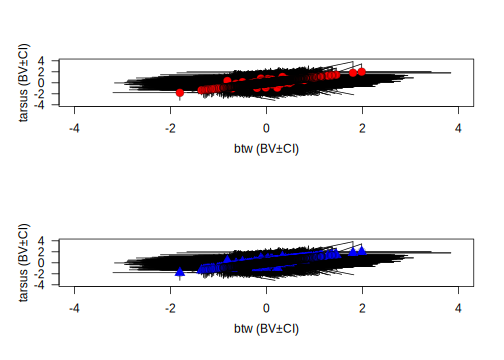
\includegraphics{wam_tuto_files/figure-latex/unnamed-chunk-136-1.pdf}

\begin{Shaded}
\begin{Highlighting}[]
\CommentTok{\#}
\end{Highlighting}
\end{Shaded}

\hypertarget{between-groups-covariances-and-the-b-matrix-1}{%
\subsection{Between groups (co)variances and the B-matrix}\label{between-groups-covariances-and-the-b-matrix-1}}

Animal models are amazing model. With different group within a population, it is also possible to estimate how much the different groups shared the same genetic via the cross-group genetic covariance.
This covariance is essential to understand ontogenic or sexual conflict, which can constraint or enhanced response to evolution.
As an example, we estimate the cross-sex genetic correlation \texttt{r\_\{fm\}}

First, we need to dissociate the trait values for females and males into distinct variables. Then, we use a bivariate model (for one trait: \texttt{tarsus}) and a multivariate model (for various traits: \texttt{tarsus} and \texttt{bwt}). With a multivariate model, the cross-sex-cross trait covariance matrix is also named \texttt{B\ matrix}.

The coding is a bit complain but pretty straightforward. It is important to modify the covariance matrix at the residual level to avoid the calculation of a cross-sex residual covariance (no individual switched sex during the experiment).

\begin{Shaded}
\begin{Highlighting}[]
\NormalTok{gryphon2}\OperatorTok{$}\NormalTok{bwt}\FloatTok{.1}\NormalTok{ \textless{}{-}}\StringTok{ }\OtherTok{NA}
\NormalTok{gryphon2}\OperatorTok{$}\NormalTok{tarsus}\FloatTok{.1}\NormalTok{ \textless{}{-}}\StringTok{ }\OtherTok{NA}
\NormalTok{animal \textless{}{-}}\StringTok{ }\NormalTok{gryphon2[gryphon2}\OperatorTok{$}\NormalTok{sex }\OperatorTok{==}\StringTok{ "1"}\NormalTok{, ]}\OperatorTok{$}\NormalTok{animal}
\ControlFlowTok{for}\NormalTok{ (i }\ControlFlowTok{in} \KeywordTok{unique}\NormalTok{(animal)) \{}
\NormalTok{  gryphon2}\OperatorTok{$}\NormalTok{bwt}\FloatTok{.1}\NormalTok{[}\KeywordTok{which}\NormalTok{(gryphon2}\OperatorTok{$}\NormalTok{animal }\OperatorTok{==}\StringTok{ }\NormalTok{i)] \textless{}{-}}\StringTok{ }\NormalTok{gryphon2}\OperatorTok{$}\NormalTok{bwt[}\KeywordTok{which}\NormalTok{(gryphon2}\OperatorTok{$}\NormalTok{animal }\OperatorTok{==}\StringTok{ }\NormalTok{i)]}
\NormalTok{  gryphon2}\OperatorTok{$}\NormalTok{tarsus}\FloatTok{.1}\NormalTok{[}\KeywordTok{which}\NormalTok{(gryphon2}\OperatorTok{$}\NormalTok{animal }\OperatorTok{==}\StringTok{ }\NormalTok{i)] \textless{}{-}}\StringTok{ }\NormalTok{gryphon2}\OperatorTok{$}\NormalTok{tarsus[}\KeywordTok{which}\NormalTok{(gryphon2}\OperatorTok{$}\NormalTok{animal }\OperatorTok{==}\StringTok{ }\NormalTok{i)]}
\NormalTok{\}}
\CommentTok{\#}
\NormalTok{gryphon2}\OperatorTok{$}\NormalTok{bwt}\FloatTok{.2}\NormalTok{ \textless{}{-}}\StringTok{ }\OtherTok{NA}
\NormalTok{gryphon2}\OperatorTok{$}\NormalTok{tarsus}\FloatTok{.2}\NormalTok{ \textless{}{-}}\StringTok{ }\OtherTok{NA}
\NormalTok{animal \textless{}{-}}\StringTok{ }\NormalTok{gryphon2[gryphon2}\OperatorTok{$}\NormalTok{sex }\OperatorTok{==}\StringTok{ "2"}\NormalTok{, ]}\OperatorTok{$}\NormalTok{animal}
\ControlFlowTok{for}\NormalTok{ (i }\ControlFlowTok{in} \KeywordTok{unique}\NormalTok{(animal)) \{}
\NormalTok{  gryphon2}\OperatorTok{$}\NormalTok{bwt}\FloatTok{.2}\NormalTok{[}\KeywordTok{which}\NormalTok{(gryphon2}\OperatorTok{$}\NormalTok{animal }\OperatorTok{==}\StringTok{ }\NormalTok{i)] \textless{}{-}}\StringTok{ }\NormalTok{gryphon2}\OperatorTok{$}\NormalTok{bwt[}\KeywordTok{which}\NormalTok{(gryphon2}\OperatorTok{$}\NormalTok{animal }\OperatorTok{==}\StringTok{ }\NormalTok{i)]}
\NormalTok{  gryphon2}\OperatorTok{$}\NormalTok{tarsus}\FloatTok{.2}\NormalTok{[}\KeywordTok{which}\NormalTok{(gryphon2}\OperatorTok{$}\NormalTok{animal }\OperatorTok{==}\StringTok{ }\NormalTok{i)] \textless{}{-}}\StringTok{ }\NormalTok{gryphon2}\OperatorTok{$}\NormalTok{tarsus[}\KeywordTok{which}\NormalTok{(gryphon2}\OperatorTok{$}\NormalTok{animal }\OperatorTok{==}\StringTok{ }\NormalTok{i)]}
\NormalTok{\}}

\CommentTok{\#}
\NormalTok{prior2}\FloatTok{.4}\NormalTok{ \textless{}{-}}\StringTok{ }\KeywordTok{list}\NormalTok{(}
  \DataTypeTok{G =} \KeywordTok{list}\NormalTok{(}
    \DataTypeTok{G1 =} \KeywordTok{list}\NormalTok{(}\DataTypeTok{V =} \KeywordTok{diag}\NormalTok{(}\DecValTok{2}\NormalTok{), }\DataTypeTok{nu =} \FloatTok{1.002}\NormalTok{),}
    \DataTypeTok{G2 =} \KeywordTok{list}\NormalTok{(}\DataTypeTok{V =} \KeywordTok{diag}\NormalTok{(}\DecValTok{2}\NormalTok{), }\DataTypeTok{nu =} \FloatTok{1.002}\NormalTok{),}
    \DataTypeTok{G3 =} \KeywordTok{list}\NormalTok{(}\DataTypeTok{V =} \KeywordTok{diag}\NormalTok{(}\DecValTok{2}\NormalTok{), }\DataTypeTok{nu =} \FloatTok{1.002}\NormalTok{)}
\NormalTok{  ),}
  \DataTypeTok{R =} \KeywordTok{list}\NormalTok{(}
    \DataTypeTok{V1 =} \KeywordTok{list}\NormalTok{(}\DataTypeTok{V =} \KeywordTok{diag}\NormalTok{(}\DecValTok{2}\NormalTok{), }\DataTypeTok{nu =} \FloatTok{1.002}\NormalTok{)}
\NormalTok{  )}
\NormalTok{)}
\CommentTok{\#}
\NormalTok{model.BivSex \textless{}{-}}\StringTok{ }\KeywordTok{MCMCglmm}\NormalTok{(}\KeywordTok{cbind}\NormalTok{(tarsus}\FloatTok{.1}\NormalTok{, tarsus}\FloatTok{.2}\NormalTok{) }\OperatorTok{\textasciitilde{}}\StringTok{ }\NormalTok{trait }\OperatorTok{{-}}\StringTok{ }\DecValTok{1}\NormalTok{,}
  \DataTypeTok{random =} \OperatorTok{\textasciitilde{}}\StringTok{ }\KeywordTok{us}\NormalTok{(trait)}\OperatorTok{:}\NormalTok{animal }\OperatorTok{+}\StringTok{ }\KeywordTok{idh}\NormalTok{(trait)}\OperatorTok{:}\NormalTok{byear }\OperatorTok{+}\StringTok{ }\KeywordTok{idh}\NormalTok{(trait)}\OperatorTok{:}\NormalTok{mother,}
  \DataTypeTok{rcov =} \OperatorTok{\textasciitilde{}}\StringTok{ }\KeywordTok{us}\NormalTok{(trait)}\OperatorTok{:}\NormalTok{units,}
  \DataTypeTok{family =} \KeywordTok{c}\NormalTok{(}\StringTok{"gaussian"}\NormalTok{, }\StringTok{"gaussian"}\NormalTok{),}
  \DataTypeTok{ginv =} \KeywordTok{list}\NormalTok{(}\DataTypeTok{animal =}\NormalTok{ Ainv), }\DataTypeTok{data =}\NormalTok{ gryphon2,}
  \DataTypeTok{nitt =} \DecValTok{130000}\NormalTok{, }\DataTypeTok{thin =} \DecValTok{100}\NormalTok{, }\DataTypeTok{burnin =} \DecValTok{30000}\NormalTok{,}
  \DataTypeTok{prior =}\NormalTok{ prior2}\FloatTok{.4}\NormalTok{, }\DataTypeTok{verbose =} \OtherTok{FALSE}\NormalTok{, }\DataTypeTok{pr =} \OtherTok{TRUE}
\NormalTok{)}

\KeywordTok{save}\NormalTok{(model.BivSex, }\DataTypeTok{file =} \StringTok{"data/MCMCglmm\_model\_BivSex\_LongRun.rda"}\NormalTok{)}
\end{Highlighting}
\end{Shaded}

Again we have provided the data from one such run. It can be accessed using the code:

\begin{Shaded}
\begin{Highlighting}[]
\KeywordTok{load}\NormalTok{(}\DataTypeTok{file =} \StringTok{"data/MCMCglmm\_model\_BivSex\_LongRun.rda"}\NormalTok{)}
\KeywordTok{summary}\NormalTok{(model.BivSex)}
\end{Highlighting}
\end{Shaded}

\begin{verbatim}
## 
##  Iterations = 30001:129901
##  Thinning interval  = 100
##  Sample size  = 1000 
## 
##  DIC: 1670.599 
## 
##  G-structure:  ~us(trait):animal
## 
##                                    post.mean l-95% CI u-95% CI eff.samp
## traittarsus.1:traittarsus.1.animal     6.632    2.136    12.69    85.74
## traittarsus.2:traittarsus.1.animal     8.043    2.389    13.54   117.04
## traittarsus.1:traittarsus.2.animal     8.043    2.389    13.54   117.04
## traittarsus.2:traittarsus.2.animal    16.145    3.128    28.93    21.81
## 
##                ~idh(trait):byear
## 
##                     post.mean l-95% CI u-95% CI eff.samp
## traittarsus.1.byear     3.184    0.505    6.515    357.4
## traittarsus.2.byear     4.576    1.346    8.476    442.5
## 
##                ~idh(trait):mother
## 
##                      post.mean l-95% CI u-95% CI eff.samp
## traittarsus.1.mother     1.777  0.07858    4.714   299.68
## traittarsus.2.mother     2.980  0.12204    7.328    70.26
## 
##  R-structure:  ~us(trait):units
## 
##                                   post.mean l-95% CI u-95% CI eff.samp
## traittarsus.1:traittarsus.1.units    15.455    8.998    21.84  104.923
## traittarsus.2:traittarsus.1.units    -1.497  -15.500    15.53    8.767
## traittarsus.1:traittarsus.2.units    -1.497  -15.500    15.53    8.767
## traittarsus.2:traittarsus.2.units     9.356    0.239    19.10   21.548
## 
##  Location effects: cbind(tarsus.1, tarsus.2) ~ trait - 1 
## 
##               post.mean l-95% CI u-95% CI eff.samp  pMCMC    
## traittarsus.1     20.48    19.62    21.48    703.9 <0.001 ***
## traittarsus.2     20.46    19.42    21.40    846.8 <0.001 ***
## ---
## Signif. codes:  0 '***' 0.001 '**' 0.01 '*' 0.05 '.' 0.1 ' ' 1
\end{verbatim}

\begin{Shaded}
\begin{Highlighting}[]
\KeywordTok{autocorr}\NormalTok{(model.BivSex}\OperatorTok{$}\NormalTok{VCV)}
\end{Highlighting}
\end{Shaded}

\begin{verbatim}
## , , traittarsus.1:traittarsus.1.animal
## 
##          traittarsus.1:traittarsus.1.animal traittarsus.2:traittarsus.1.animal
## Lag 0                            1.00000000                         0.48422763
## Lag 100                          0.73797990                         0.27701934
## Lag 500                          0.43151596                         0.08460564
## Lag 1000                         0.27709357                         0.03138071
## Lag 5000                         0.09623473                         0.02508175
##          traittarsus.1:traittarsus.2.animal traittarsus.2:traittarsus.2.animal
## Lag 0                            0.48422763                        -0.20835012
## Lag 100                          0.27701934                        -0.26518087
## Lag 500                          0.08460564                        -0.27929151
## Lag 1000                         0.03138071                        -0.23408954
## Lag 5000                         0.02508175                        -0.02431482
##          traittarsus.1.byear traittarsus.2.byear traittarsus.1.mother
## Lag 0             0.05650214        -0.059474225         -0.038396947
## Lag 100           0.03805347        -0.063250151         -0.012779432
## Lag 500           0.03353186        -0.031583736          0.059794328
## Lag 1000          0.02971111         0.032191172         -0.004310584
## Lag 5000          0.04021796        -0.001198619         -0.065221991
##          traittarsus.2.mother traittarsus.1:traittarsus.1.units
## Lag 0               0.1285643                        -0.7394524
## Lag 100             0.1416089                        -0.5874113
## Lag 500             0.1227812                        -0.3892610
## Lag 1000            0.1054744                        -0.2272794
## Lag 5000            0.1046093                        -0.0490914
##          traittarsus.2:traittarsus.1.units traittarsus.1:traittarsus.2.units
## Lag 0                         -0.030661923                      -0.030661923
## Lag 100                       -0.009066847                      -0.009066847
## Lag 500                       -0.014021640                      -0.014021640
## Lag 1000                      -0.038727365                      -0.038727365
## Lag 5000                      -0.053406989                      -0.053406989
##          traittarsus.2:traittarsus.2.units
## Lag 0                           0.24444681
## Lag 100                         0.28630940
## Lag 500                         0.28676382
## Lag 1000                        0.25016902
## Lag 5000                       -0.01889626
## 
## , , traittarsus.2:traittarsus.1.animal
## 
##          traittarsus.1:traittarsus.1.animal traittarsus.2:traittarsus.1.animal
## Lag 0                            0.48422763                         1.00000000
## Lag 100                          0.25316393                         0.68722653
## Lag 500                         -0.01525426                         0.30994286
## Lag 1000                        -0.13117432                         0.12750201
## Lag 5000                        -0.03481149                         0.01967858
##          traittarsus.1:traittarsus.2.animal traittarsus.2:traittarsus.2.animal
## Lag 0                            1.00000000                          0.4372811
## Lag 100                          0.68722653                          0.3171927
## Lag 500                          0.30994286                          0.2173200
## Lag 1000                         0.12750201                          0.2034517
## Lag 5000                         0.01967858                          0.1155543
##          traittarsus.1.byear traittarsus.2.byear traittarsus.1.mother
## Lag 0           -0.028123268         -0.10117282          0.068035501
## Lag 100         -0.036441213         -0.06326083          0.058376180
## Lag 500         -0.017206400         -0.06159010         -0.002869166
## Lag 1000        -0.004346341          0.06173108         -0.017320527
## Lag 5000        -0.044798021          0.07734401         -0.083350187
##          traittarsus.2.mother traittarsus.1:traittarsus.1.units
## Lag 0            -0.261520775                       -0.32691256
## Lag 100          -0.219989670                       -0.19037150
## Lag 500          -0.171008994                        0.03568009
## Lag 1000         -0.073253782                        0.15052971
## Lag 5000         -0.002628408                        0.06147675
##          traittarsus.2:traittarsus.1.units traittarsus.1:traittarsus.2.units
## Lag 0                          -0.15561461                       -0.15561461
## Lag 100                        -0.11940169                       -0.11940169
## Lag 500                        -0.10722180                       -0.10722180
## Lag 1000                       -0.11888700                       -0.11888700
## Lag 5000                       -0.07749379                       -0.07749379
##          traittarsus.2:traittarsus.2.units
## Lag 0                           -0.3304177
## Lag 100                         -0.2624116
## Lag 500                         -0.1893048
## Lag 1000                        -0.2045441
## Lag 5000                        -0.1580773
## 
## , , traittarsus.1:traittarsus.2.animal
## 
##          traittarsus.1:traittarsus.1.animal traittarsus.2:traittarsus.1.animal
## Lag 0                            0.48422763                         1.00000000
## Lag 100                          0.25316393                         0.68722653
## Lag 500                         -0.01525426                         0.30994286
## Lag 1000                        -0.13117432                         0.12750201
## Lag 5000                        -0.03481149                         0.01967858
##          traittarsus.1:traittarsus.2.animal traittarsus.2:traittarsus.2.animal
## Lag 0                            1.00000000                          0.4372811
## Lag 100                          0.68722653                          0.3171927
## Lag 500                          0.30994286                          0.2173200
## Lag 1000                         0.12750201                          0.2034517
## Lag 5000                         0.01967858                          0.1155543
##          traittarsus.1.byear traittarsus.2.byear traittarsus.1.mother
## Lag 0           -0.028123268         -0.10117282          0.068035501
## Lag 100         -0.036441213         -0.06326083          0.058376180
## Lag 500         -0.017206400         -0.06159010         -0.002869166
## Lag 1000        -0.004346341          0.06173108         -0.017320527
## Lag 5000        -0.044798021          0.07734401         -0.083350187
##          traittarsus.2.mother traittarsus.1:traittarsus.1.units
## Lag 0            -0.261520775                       -0.32691256
## Lag 100          -0.219989670                       -0.19037150
## Lag 500          -0.171008994                        0.03568009
## Lag 1000         -0.073253782                        0.15052971
## Lag 5000         -0.002628408                        0.06147675
##          traittarsus.2:traittarsus.1.units traittarsus.1:traittarsus.2.units
## Lag 0                          -0.15561461                       -0.15561461
## Lag 100                        -0.11940169                       -0.11940169
## Lag 500                        -0.10722180                       -0.10722180
## Lag 1000                       -0.11888700                       -0.11888700
## Lag 5000                       -0.07749379                       -0.07749379
##          traittarsus.2:traittarsus.2.units
## Lag 0                           -0.3304177
## Lag 100                         -0.2624116
## Lag 500                         -0.1893048
## Lag 1000                        -0.2045441
## Lag 5000                        -0.1580773
## 
## , , traittarsus.2:traittarsus.2.animal
## 
##          traittarsus.1:traittarsus.1.animal traittarsus.2:traittarsus.1.animal
## Lag 0                            -0.2083501                         0.43728107
## Lag 100                          -0.2828015                         0.29272735
## Lag 500                          -0.3313152                         0.14658444
## Lag 1000                         -0.3483078                         0.06012732
## Lag 5000                         -0.1542996                        -0.06471744
##          traittarsus.1:traittarsus.2.animal traittarsus.2:traittarsus.2.animal
## Lag 0                            0.43728107                         1.00000000
## Lag 100                          0.29272735                         0.87775419
## Lag 500                          0.14658444                         0.72227084
## Lag 1000                         0.06012732                         0.61062886
## Lag 5000                        -0.06471744                         0.08074184
##          traittarsus.1.byear traittarsus.2.byear traittarsus.1.mother
## Lag 0           -0.020084226        -0.013645105          0.007263224
## Lag 100         -0.015303798         0.015235251          0.013922907
## Lag 500         -0.009604004        -0.004276257         -0.022794079
## Lag 1000        -0.036443873         0.045216146          0.038406389
## Lag 5000        -0.046131641         0.012581835         -0.012187074
##          traittarsus.2.mother traittarsus.1:traittarsus.1.units
## Lag 0             -0.50677816                        0.23024103
## Lag 100           -0.46549011                        0.26517948
## Lag 500           -0.35999881                        0.31894466
## Lag 1000          -0.26148886                        0.30787546
## Lag 5000          -0.09601646                        0.09998448
##          traittarsus.2:traittarsus.1.units traittarsus.1:traittarsus.2.units
## Lag 0                           0.03215520                        0.03215520
## Lag 100                         0.04234930                        0.04234930
## Lag 500                         0.01485912                        0.01485912
## Lag 1000                       -0.02777646                       -0.02777646
## Lag 5000                       -0.10000281                       -0.10000281
##          traittarsus.2:traittarsus.2.units
## Lag 0                          -0.90778147
## Lag 100                        -0.84400702
## Lag 500                        -0.70957533
## Lag 1000                       -0.62450980
## Lag 5000                       -0.06262314
## 
## , , traittarsus.1.byear
## 
##          traittarsus.1:traittarsus.1.animal traittarsus.2:traittarsus.1.animal
## Lag 0                            0.05650214                        -0.02812327
## Lag 100                          0.06068975                        -0.02687949
## Lag 500                          0.02342116                        -0.03285780
## Lag 1000                         0.03532201                        -0.03419221
## Lag 5000                         0.02786557                        -0.01481811
##          traittarsus.1:traittarsus.2.animal traittarsus.2:traittarsus.2.animal
## Lag 0                           -0.02812327                        -0.02008423
## Lag 100                         -0.02687949                        -0.02175035
## Lag 500                         -0.03285780                        -0.01196604
## Lag 1000                        -0.03419221                        -0.03085934
## Lag 5000                        -0.01481811                         0.01496886
##          traittarsus.1.byear traittarsus.2.byear traittarsus.1.mother
## Lag 0             1.00000000        -0.008840935         -0.034026465
## Lag 100           0.23201455        -0.040849216          0.006952432
## Lag 500           0.10173419         0.018677216          0.021915445
## Lag 1000          0.05656314         0.045347703         -0.069023041
## Lag 5000         -0.02674433         0.003879773         -0.031727649
##          traittarsus.2.mother traittarsus.1:traittarsus.1.units
## Lag 0             0.041524616                      -0.131561587
## Lag 100           0.022654125                      -0.091920671
## Lag 500          -0.003137523                      -0.023174815
## Lag 1000          0.093233105                       0.017723781
## Lag 5000         -0.001576843                       0.003971118
##          traittarsus.2:traittarsus.1.units traittarsus.1:traittarsus.2.units
## Lag 0                           0.06264243                        0.06264243
## Lag 100                         0.06240060                        0.06240060
## Lag 500                         0.03789653                        0.03789653
## Lag 1000                        0.03352306                        0.03352306
## Lag 5000                        0.05768588                        0.05768588
##          traittarsus.2:traittarsus.2.units
## Lag 0                          0.013826338
## Lag 100                        0.015690413
## Lag 500                        0.020546446
## Lag 1000                      -0.006052117
## Lag 5000                      -0.020241900
## 
## , , traittarsus.2.byear
## 
##          traittarsus.1:traittarsus.1.animal traittarsus.2:traittarsus.1.animal
## Lag 0                          -0.059474225                        -0.10117282
## Lag 100                        -0.029542673                        -0.06571088
## Lag 500                         0.019127206                         0.02553144
## Lag 1000                       -0.006675716                         0.03933732
## Lag 5000                       -0.020363086                        -0.01801919
##          traittarsus.1:traittarsus.2.animal traittarsus.2:traittarsus.2.animal
## Lag 0                           -0.10117282                       -0.013645105
## Lag 100                         -0.06571088                       -0.001743299
## Lag 500                          0.02553144                        0.024080673
## Lag 1000                         0.03933732                        0.020998801
## Lag 5000                        -0.01801919                       -0.036422613
##          traittarsus.1.byear traittarsus.2.byear traittarsus.1.mother
## Lag 0           -0.008840935          1.00000000          0.019871390
## Lag 100          0.003895756          0.15813110          0.000200299
## Lag 500         -0.028206511          0.02861588          0.028238837
## Lag 1000        -0.022327614          0.02577769          0.069995240
## Lag 5000         0.054519302         -0.01863939          0.021348106
##          traittarsus.2.mother traittarsus.1:traittarsus.1.units
## Lag 0              0.02790731                        0.04582166
## Lag 100           -0.02533496                        0.01584625
## Lag 500           -0.04228406                       -0.01965332
## Lag 1000          -0.03776489                       -0.05592538
## Lag 5000           0.04026220                        0.02293994
##          traittarsus.2:traittarsus.1.units traittarsus.1:traittarsus.2.units
## Lag 0                          -0.01692229                       -0.01692229
## Lag 100                        -0.03014201                       -0.03014201
## Lag 500                        -0.05685394                       -0.05685394
## Lag 1000                       -0.05775898                       -0.05775898
## Lag 5000                       -0.04474406                       -0.04474406
##          traittarsus.2:traittarsus.2.units
## Lag 0                          -0.05647151
## Lag 100                        -0.01120227
## Lag 500                        -0.02826105
## Lag 1000                       -0.01902149
## Lag 5000                        0.04653422
## 
## , , traittarsus.1.mother
## 
##          traittarsus.1:traittarsus.1.animal traittarsus.2:traittarsus.1.animal
## Lag 0                           -0.03839695                        0.068035501
## Lag 100                         -0.01125448                        0.090872487
## Lag 500                         -0.01822303                        0.074904451
## Lag 1000                        -0.06684368                       -0.009049799
## Lag 5000                         0.01882807                       -0.038704215
##          traittarsus.1:traittarsus.2.animal traittarsus.2:traittarsus.2.animal
## Lag 0                           0.068035501                        0.007263224
## Lag 100                         0.090872487                        0.009427782
## Lag 500                         0.074904451                       -0.008966636
## Lag 1000                       -0.009049799                       -0.062208885
## Lag 5000                       -0.038704215                       -0.090802212
##          traittarsus.1.byear traittarsus.2.byear traittarsus.1.mother
## Lag 0           -0.034026465         0.019871390           1.00000000
## Lag 100         -0.044009625        -0.022642909           0.53848292
## Lag 500          0.033149894        -0.058758981           0.05060514
## Lag 1000        -0.034811076        -0.041691079          -0.01263351
## Lag 5000         0.003520887        -0.007417182          -0.01561154
##          traittarsus.2.mother traittarsus.1:traittarsus.1.units
## Lag 0            -0.053312892                      -0.274551627
## Lag 100          -0.021399368                      -0.183188795
## Lag 500           0.001127949                      -0.004741630
## Lag 1000          0.017008055                       0.049168722
## Lag 5000         -0.013865361                      -0.003898312
##          traittarsus.2:traittarsus.1.units traittarsus.1:traittarsus.2.units
## Lag 0                          0.021389916                       0.021389916
## Lag 100                        0.010504830                       0.010504830
## Lag 500                        0.005067944                       0.005067944
## Lag 1000                       0.024425517                       0.024425517
## Lag 5000                      -0.004626176                      -0.004626176
##          traittarsus.2:traittarsus.2.units
## Lag 0                           0.02429791
## Lag 100                         0.01285473
## Lag 500                         0.02017728
## Lag 1000                        0.06093906
## Lag 5000                        0.10720949
## 
## , , traittarsus.2.mother
## 
##          traittarsus.1:traittarsus.1.animal traittarsus.2:traittarsus.1.animal
## Lag 0                            0.12856434                         -0.2615208
## Lag 100                          0.14693139                         -0.2325836
## Lag 500                          0.21342005                         -0.1621874
## Lag 1000                         0.23353394                         -0.1119149
## Lag 5000                         0.02771044                          0.0396288
##          traittarsus.1:traittarsus.2.animal traittarsus.2:traittarsus.2.animal
## Lag 0                            -0.2615208                        -0.50677816
## Lag 100                          -0.2325836                        -0.48725853
## Lag 500                          -0.1621874                        -0.40888208
## Lag 1000                         -0.1119149                        -0.34699264
## Lag 5000                          0.0396288                         0.02549716
##          traittarsus.1.byear traittarsus.2.byear traittarsus.1.mother
## Lag 0             0.04152462         0.027907314          -0.05331289
## Lag 100           0.02194445         0.054336046          -0.04284508
## Lag 500          -0.03327513        -0.020857444          -0.02968159
## Lag 1000          0.02573536        -0.040238713          -0.03336616
## Lag 5000          0.01374507         0.005808512           0.07687084
##          traittarsus.2.mother traittarsus.1:traittarsus.1.units
## Lag 0              1.00000000                       -0.13910701
## Lag 100            0.70222369                       -0.13691118
## Lag 500            0.35625516                       -0.18735521
## Lag 1000           0.19638031                       -0.21082439
## Lag 5000          -0.04114072                       -0.04387536
##          traittarsus.2:traittarsus.1.units traittarsus.1:traittarsus.2.units
## Lag 0                           0.04614450                        0.04614450
## Lag 100                         0.04486226                        0.04486226
## Lag 500                         0.04022585                        0.04022585
## Lag 1000                        0.05277963                        0.05277963
## Lag 5000                        0.04252673                        0.04252673
##          traittarsus.2:traittarsus.2.units
## Lag 0                          0.268960307
## Lag 100                        0.289158808
## Lag 500                        0.345252707
## Lag 1000                       0.323960441
## Lag 5000                      -0.002082367
## 
## , , traittarsus.1:traittarsus.1.units
## 
##          traittarsus.1:traittarsus.1.animal traittarsus.2:traittarsus.1.animal
## Lag 0                            -0.7394524                        -0.32691256
## Lag 100                          -0.5906993                        -0.20009588
## Lag 500                          -0.3828210                        -0.08127245
## Lag 1000                         -0.2031251                         0.02298348
## Lag 5000                         -0.0979703                        -0.01920779
##          traittarsus.1:traittarsus.2.animal traittarsus.2:traittarsus.2.animal
## Lag 0                           -0.32691256                         0.23024103
## Lag 100                         -0.20009588                         0.28084172
## Lag 500                         -0.08127245                         0.28272296
## Lag 1000                         0.02298348                         0.28283381
## Lag 5000                        -0.01920779                         0.05177093
##          traittarsus.1.byear traittarsus.2.byear traittarsus.1.mother
## Lag 0            -0.13156159          0.04582166          -0.27455163
## Lag 100          -0.05719958          0.04337991          -0.16825519
## Lag 500          -0.06997182          0.07140946          -0.07087194
## Lag 1000         -0.02088140          0.01426241           0.03955072
## Lag 5000         -0.01887279          0.04431921           0.06767122
##          traittarsus.2.mother traittarsus.1:traittarsus.1.units
## Lag 0              -0.1391070                        1.00000000
## Lag 100            -0.1379410                        0.56579808
## Lag 500            -0.1301093                        0.35250381
## Lag 1000           -0.1253506                        0.15585076
## Lag 5000           -0.0735286                        0.05909602
##          traittarsus.2:traittarsus.1.units traittarsus.1:traittarsus.2.units
## Lag 0                           0.04896537                        0.04896537
## Lag 100                         0.02746645                        0.02746645
## Lag 500                         0.03218528                        0.03218528
## Lag 1000                        0.05596211                        0.05596211
## Lag 5000                        0.05413531                        0.05413531
##          traittarsus.2:traittarsus.2.units
## Lag 0                           -0.2610614
## Lag 100                         -0.3079509
## Lag 500                         -0.2969894
## Lag 1000                        -0.2847495
## Lag 5000                        -0.0427216
## 
## , , traittarsus.2:traittarsus.1.units
## 
##          traittarsus.1:traittarsus.1.animal traittarsus.2:traittarsus.1.animal
## Lag 0                          -0.030661923                        -0.15561461
## Lag 100                         0.003884354                        -0.11920858
## Lag 500                         0.042099074                        -0.08915914
## Lag 1000                        0.042025296                        -0.07981143
## Lag 5000                       -0.018911064                        -0.09774452
##          traittarsus.1:traittarsus.2.animal traittarsus.2:traittarsus.2.animal
## Lag 0                           -0.15561461                         0.03215520
## Lag 100                         -0.11920858                         0.04834806
## Lag 500                         -0.08915914                         0.05802195
## Lag 1000                        -0.07981143                         0.02656239
## Lag 5000                        -0.09774452                        -0.04245498
##          traittarsus.1.byear traittarsus.2.byear traittarsus.1.mother
## Lag 0             0.06264243        -0.016922288           0.02138992
## Lag 100           0.06751797        -0.004991909           0.02085557
## Lag 500           0.06731777        -0.030284706           0.05500122
## Lag 1000          0.06629827        -0.044495833           0.10333723
## Lag 5000          0.08927471        -0.038637660           0.06016204
##          traittarsus.2.mother traittarsus.1:traittarsus.1.units
## Lag 0              0.04614450                       0.048965370
## Lag 100            0.04880037                       0.017340477
## Lag 500            0.04329157                      -0.013844496
## Lag 1000           0.06724925                      -0.039591736
## Lag 5000           0.04795409                      -0.003568665
##          traittarsus.2:traittarsus.1.units traittarsus.1:traittarsus.2.units
## Lag 0                            1.0000000                         1.0000000
## Lag 100                          0.9675526                         0.9675526
## Lag 500                          0.9029928                         0.9029928
## Lag 1000                         0.8401123                         0.8401123
## Lag 5000                         0.4663345                         0.4663345
##          traittarsus.2:traittarsus.2.units
## Lag 0                          -0.04275237
## Lag 100                        -0.06227874
## Lag 500                        -0.06672641
## Lag 1000                       -0.04382724
## Lag 5000                        0.03699475
## 
## , , traittarsus.1:traittarsus.2.units
## 
##          traittarsus.1:traittarsus.1.animal traittarsus.2:traittarsus.1.animal
## Lag 0                          -0.030661923                        -0.15561461
## Lag 100                         0.003884354                        -0.11920858
## Lag 500                         0.042099074                        -0.08915914
## Lag 1000                        0.042025296                        -0.07981143
## Lag 5000                       -0.018911064                        -0.09774452
##          traittarsus.1:traittarsus.2.animal traittarsus.2:traittarsus.2.animal
## Lag 0                           -0.15561461                         0.03215520
## Lag 100                         -0.11920858                         0.04834806
## Lag 500                         -0.08915914                         0.05802195
## Lag 1000                        -0.07981143                         0.02656239
## Lag 5000                        -0.09774452                        -0.04245498
##          traittarsus.1.byear traittarsus.2.byear traittarsus.1.mother
## Lag 0             0.06264243        -0.016922288           0.02138992
## Lag 100           0.06751797        -0.004991909           0.02085557
## Lag 500           0.06731777        -0.030284706           0.05500122
## Lag 1000          0.06629827        -0.044495833           0.10333723
## Lag 5000          0.08927471        -0.038637660           0.06016204
##          traittarsus.2.mother traittarsus.1:traittarsus.1.units
## Lag 0              0.04614450                       0.048965370
## Lag 100            0.04880037                       0.017340477
## Lag 500            0.04329157                      -0.013844496
## Lag 1000           0.06724925                      -0.039591736
## Lag 5000           0.04795409                      -0.003568665
##          traittarsus.2:traittarsus.1.units traittarsus.1:traittarsus.2.units
## Lag 0                            1.0000000                         1.0000000
## Lag 100                          0.9675526                         0.9675526
## Lag 500                          0.9029928                         0.9029928
## Lag 1000                         0.8401123                         0.8401123
## Lag 5000                         0.4663345                         0.4663345
##          traittarsus.2:traittarsus.2.units
## Lag 0                          -0.04275237
## Lag 100                        -0.06227874
## Lag 500                        -0.06672641
## Lag 1000                       -0.04382724
## Lag 5000                        0.03699475
## 
## , , traittarsus.2:traittarsus.2.units
## 
##          traittarsus.1:traittarsus.1.animal traittarsus.2:traittarsus.1.animal
## Lag 0                             0.2444468                        -0.33041768
## Lag 100                           0.2953169                        -0.24524259
## Lag 500                           0.3257997                        -0.12021844
## Lag 1000                          0.3204576                        -0.05040170
## Lag 5000                          0.1966910                         0.07386444
##          traittarsus.1:traittarsus.2.animal traittarsus.2:traittarsus.2.animal
## Lag 0                           -0.33041768                         -0.9077815
## Lag 100                         -0.24524259                         -0.8410651
## Lag 500                         -0.12021844                         -0.6969304
## Lag 1000                        -0.05040170                         -0.5893775
## Lag 5000                         0.07386444                         -0.1004775
##          traittarsus.1.byear traittarsus.2.byear traittarsus.1.mother
## Lag 0             0.01382634        -0.056471508          0.024297909
## Lag 100           0.01730830        -0.030701856          0.017739447
## Lag 500           0.03968933         0.004065694          0.010636299
## Lag 1000          0.03341332        -0.048898719         -0.028816725
## Lag 5000          0.05219060        -0.013503372         -0.005167407
##          traittarsus.2.mother traittarsus.1:traittarsus.1.units
## Lag 0               0.2689603                        -0.2610614
## Lag 100             0.3013532                        -0.3031510
## Lag 500             0.3094825                        -0.3179085
## Lag 1000            0.2400190                        -0.2838200
## Lag 5000            0.1233946                        -0.1252443
##          traittarsus.2:traittarsus.1.units traittarsus.1:traittarsus.2.units
## Lag 0                          -0.04275237                       -0.04275237
## Lag 100                        -0.05037125                       -0.05037125
## Lag 500                        -0.01879502                       -0.01879502
## Lag 1000                        0.02100080                        0.02100080
## Lag 5000                        0.10654662                        0.10654662
##          traittarsus.2:traittarsus.2.units
## Lag 0                           1.00000000
## Lag 100                         0.87986649
## Lag 500                         0.70214749
## Lag 1000                        0.61035106
## Lag 5000                        0.07522425
\end{verbatim}

The cross-sex genetic correlation can estimate form the output of the model.
For tarsus length at fledging, sexes shared a lot of genetic variance which is commun for a trait with low sexual dimorphism. If the selection is antagonistic between males and females, sexes can not evolve freely form the other sexes and a sexual conflict appears.

\begin{Shaded}
\begin{Highlighting}[]
\NormalTok{rfm \textless{}{-}}\StringTok{ }\NormalTok{model.BivSex}\OperatorTok{$}\NormalTok{VCV[, }\StringTok{"traittarsus.1:traittarsus.2.animal"}\NormalTok{] }\OperatorTok{/}\StringTok{ }\KeywordTok{sqrt}\NormalTok{(model.BivSex}\OperatorTok{$}\NormalTok{VCV[, }\StringTok{"traittarsus.1:traittarsus.1.animal"}\NormalTok{] }\OperatorTok{*}\StringTok{ }\NormalTok{model.BivSex}\OperatorTok{$}\NormalTok{VCV[, }\StringTok{"traittarsus.2:traittarsus.2.animal"}\NormalTok{])}
\KeywordTok{posterior.mode}\NormalTok{(rfm)}
\end{Highlighting}
\end{Shaded}

\begin{verbatim}
##      var1 
## 0.9664439
\end{verbatim}

\begin{Shaded}
\begin{Highlighting}[]
\KeywordTok{HPDinterval}\NormalTok{(rfm, }\FloatTok{0.95}\NormalTok{)}
\end{Highlighting}
\end{Shaded}

\begin{verbatim}
##          lower    upper
## var1 0.4630817 0.992376
## attr(,"Probability")
## [1] 0.95
\end{verbatim}

We can estimate directly the correlation and plot the cross-sex genetic correlation

\begin{Shaded}
\begin{Highlighting}[]
\NormalTok{DvsS \textless{}{-}}\StringTok{ }\KeywordTok{data.frame}\NormalTok{(}
  \DataTypeTok{Trait =} \KeywordTok{colnames}\NormalTok{(model.BivSex}\OperatorTok{$}\NormalTok{Sol),}
  \DataTypeTok{BLUP =} \KeywordTok{posterior.mode}\NormalTok{(model.BivSex}\OperatorTok{$}\NormalTok{Sol),}
  \DataTypeTok{CI =} \KeywordTok{HPDinterval}\NormalTok{((model.BivSex}\OperatorTok{$}\NormalTok{Sol))}
\NormalTok{)}
\NormalTok{DvsS \textless{}{-}}\StringTok{ }\NormalTok{DvsS[}\DecValTok{3}\OperatorTok{:}\DecValTok{2619}\NormalTok{, ] }\CommentTok{\# keep only rows associated with animal}
\NormalTok{DvsS}\OperatorTok{$}\NormalTok{ID \textless{}{-}}\StringTok{ }\KeywordTok{substr}\NormalTok{(DvsS}\OperatorTok{$}\NormalTok{Trait, }\DecValTok{22}\NormalTok{, }\DecValTok{26}\NormalTok{)}
\NormalTok{DvsS}\OperatorTok{$}\NormalTok{TRAIT \textless{}{-}}\StringTok{ }\KeywordTok{substr}\NormalTok{(DvsS}\OperatorTok{$}\NormalTok{Trait, }\DecValTok{6}\NormalTok{, }\DecValTok{13}\NormalTok{)}
\KeywordTok{summary}\NormalTok{(}\KeywordTok{factor}\NormalTok{(DvsS}\OperatorTok{$}\NormalTok{TRAIT))}
\end{Highlighting}
\end{Shaded}

\begin{verbatim}
## tarsus.1 tarsus.2 
##     1309     1308
\end{verbatim}

\begin{Shaded}
\begin{Highlighting}[]
\NormalTok{DvsS}\OperatorTok{$}\NormalTok{Trait \textless{}{-}}\StringTok{ }\OtherTok{NULL}
\NormalTok{BLUPS \textless{}{-}}\StringTok{ }\KeywordTok{reshape}\NormalTok{(DvsS, }\DataTypeTok{v.names =} \KeywordTok{c}\NormalTok{(}\StringTok{"BLUP"}\NormalTok{, }\StringTok{"CI.lower"}\NormalTok{, }\StringTok{"CI.upper"}\NormalTok{), }\DataTypeTok{idvar =} \StringTok{"ID"}\NormalTok{, }\DataTypeTok{timevar =} \StringTok{"TRAIT"}\NormalTok{, }\DataTypeTok{direction =} \StringTok{"wide"}\NormalTok{)}
\KeywordTok{nrow}\NormalTok{(BLUPS)}
\end{Highlighting}
\end{Shaded}

\begin{verbatim}
## [1] 1309
\end{verbatim}

\begin{Shaded}
\begin{Highlighting}[]
\KeywordTok{rownames}\NormalTok{(BLUPS) \textless{}{-}}\StringTok{ }\KeywordTok{c}\NormalTok{()}
\KeywordTok{colnames}\NormalTok{(BLUPS) \textless{}{-}}\StringTok{ }\KeywordTok{c}\NormalTok{(}\StringTok{"ID"}\NormalTok{, }\StringTok{"BLUP.btw"}\NormalTok{, }\StringTok{"CI.L.btw"}\NormalTok{, }\StringTok{"CI.U.btw"}\NormalTok{, }\StringTok{"BLUP.tarsus"}\NormalTok{, }\StringTok{"CI.L.tarsus"}\NormalTok{, }\StringTok{"CI.U.tarsus"}\NormalTok{)}
\KeywordTok{summary}\NormalTok{(BLUPS)}
\end{Highlighting}
\end{Shaded}

\begin{verbatim}
##       ID               BLUP.btw            CI.L.btw          CI.U.btw      
##  Length:1309        Min.   :-4.299559   Min.   :-9.4393   Min.   : 0.5871  
##  Class :character   1st Qu.:-0.743429   1st Qu.:-5.2018   1st Qu.: 3.5625  
##  Mode  :character   Median :-0.000879   Median :-4.3976   Median : 4.5287  
##                     Mean   : 0.024573   Mean   :-4.3251   Mean   : 4.4753  
##                     3rd Qu.: 0.762532   3rd Qu.:-3.4818   3rd Qu.: 5.3499  
##                     Max.   : 4.546380   Max.   : 0.5408   Max.   :10.9441  
##                                                                            
##   BLUP.tarsus        CI.L.tarsus       CI.U.tarsus     
##  Min.   :-8.75836   Min.   :-14.320   Min.   :-0.3279  
##  1st Qu.:-1.05894   1st Qu.: -8.157   1st Qu.: 4.9941  
##  Median : 0.06830   Median : -6.720   Median : 6.8745  
##  Mean   : 0.07182   Mean   : -6.467   Mean   : 6.6117  
##  3rd Qu.: 1.16904   3rd Qu.: -4.869   3rd Qu.: 8.3023  
##  Max.   :13.71503   Max.   :  1.264   Max.   :16.7611  
##  NA's   :1          NA's   :1         NA's   :1
\end{verbatim}

\begin{Shaded}
\begin{Highlighting}[]
\KeywordTok{plot}\NormalTok{(BLUP.tarsus }\OperatorTok{\textasciitilde{}}\StringTok{ }\NormalTok{BLUP.btw, BLUPS, }\DataTypeTok{xlab =} \StringTok{""}\NormalTok{, }\DataTypeTok{ylab =} \StringTok{""}\NormalTok{, }\DataTypeTok{las =} \FloatTok{1.2}\NormalTok{, }\DataTypeTok{bty =} \StringTok{"o"}\NormalTok{, }\DataTypeTok{col =} \StringTok{"white"}\NormalTok{)}
\KeywordTok{arrows}\NormalTok{(}\DataTypeTok{x0 =}\NormalTok{ BLUPS}\OperatorTok{$}\NormalTok{BLUP.btw, }\DataTypeTok{y0 =}\NormalTok{ BLUPS}\OperatorTok{$}\NormalTok{CI.L.tarsus, }\DataTypeTok{x1 =}\NormalTok{ BLUPS}\OperatorTok{$}\NormalTok{BLUP.btw, }\DataTypeTok{y1 =}\NormalTok{ BLUPS}\OperatorTok{$}\NormalTok{CI.U.tarsus, }\DataTypeTok{col =} \StringTok{"black"}\NormalTok{, }\DataTypeTok{code =} \DecValTok{3}\NormalTok{, }\DataTypeTok{angle =} \DecValTok{90}\NormalTok{, }\DataTypeTok{length =} \DecValTok{0}\NormalTok{)}
\KeywordTok{arrows}\NormalTok{(}\DataTypeTok{x0 =}\NormalTok{ BLUPS}\OperatorTok{$}\NormalTok{CI.L.btw, }\DataTypeTok{y0 =}\NormalTok{ BLUPS}\OperatorTok{$}\NormalTok{BLUP.tarsus, }\DataTypeTok{x1 =}\NormalTok{ BLUPS}\OperatorTok{$}\NormalTok{CI.U.btw, }\DataTypeTok{y1 =}\NormalTok{ BLUPS}\OperatorTok{$}\NormalTok{BLUP.tarsus, }\DataTypeTok{col =} \StringTok{"black"}\NormalTok{, }\DataTypeTok{code =} \DecValTok{3}\NormalTok{, }\DataTypeTok{angle =} \DecValTok{90}\NormalTok{, }\DataTypeTok{length =} \DecValTok{0}\NormalTok{)}
\KeywordTok{points}\NormalTok{(BLUP.tarsus }\OperatorTok{\textasciitilde{}}\StringTok{ }\NormalTok{BLUP.btw, BLUPS, }\DataTypeTok{pch =} \DecValTok{16}\NormalTok{, }\DataTypeTok{col =} \KeywordTok{rgb}\NormalTok{(}\DecValTok{1}\NormalTok{, }\DecValTok{0}\NormalTok{, }\DecValTok{1}\NormalTok{, }\FloatTok{0.2}\NormalTok{), }\DataTypeTok{cex =} \FloatTok{1.5}\NormalTok{)}
\KeywordTok{points}\NormalTok{(BLUP.tarsus }\OperatorTok{\textasciitilde{}}\StringTok{ }\NormalTok{BLUP.btw, BLUPS, }\DataTypeTok{pch =} \DecValTok{1}\NormalTok{, }\DataTypeTok{col =} \KeywordTok{rgb}\NormalTok{(}\DecValTok{1}\NormalTok{, }\DecValTok{0}\NormalTok{, }\DecValTok{1}\NormalTok{, }\FloatTok{0.2}\NormalTok{), }\DataTypeTok{cex =} \KeywordTok{c}\NormalTok{(}\FloatTok{1.5}\NormalTok{))}
\KeywordTok{mtext}\NormalTok{(}\StringTok{"Male tarsus (BV±CI)"}\NormalTok{, }\DataTypeTok{side =} \DecValTok{1}\NormalTok{, }\DataTypeTok{line =} \FloatTok{2.4}\NormalTok{)}
\KeywordTok{mtext}\NormalTok{(}\StringTok{"Female tarsus (BV±CI)"}\NormalTok{, }\DataTypeTok{side =} \DecValTok{2}\NormalTok{, }\DataTypeTok{line =} \DecValTok{2}\NormalTok{, }\DataTypeTok{las =} \DecValTok{3}\NormalTok{)}
\end{Highlighting}
\end{Shaded}

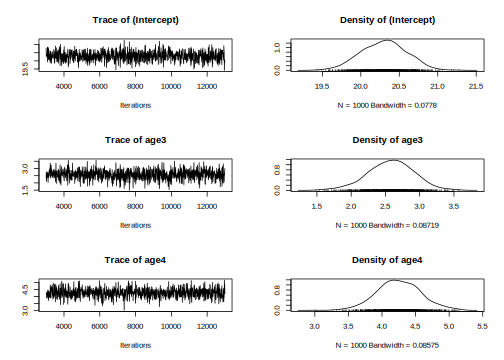
\includegraphics{wam_tuto_files/figure-latex/unnamed-chunk-140-1.pdf}

\begin{Shaded}
\begin{Highlighting}[]
\CommentTok{\#}
\end{Highlighting}
\end{Shaded}

The B matrix used the same code but in a multivariate animal model framework. Here some example code, however due to the nature of the dataset, the cross-sex genetic covariance for birth weight is hard to estimate making difficulty to fit this multivariate animal model.

\begin{Shaded}
\begin{Highlighting}[]
\NormalTok{prior2}\FloatTok{.5}\NormalTok{ \textless{}{-}}\StringTok{ }\KeywordTok{list}\NormalTok{(}
  \DataTypeTok{G =} \KeywordTok{list}\NormalTok{(}
    \DataTypeTok{G1 =} \KeywordTok{list}\NormalTok{(}\DataTypeTok{V =} \KeywordTok{diag}\NormalTok{(}\DecValTok{4}\NormalTok{), }\DataTypeTok{nu =} \FloatTok{1.002}\NormalTok{),}
    \DataTypeTok{G2 =} \KeywordTok{list}\NormalTok{(}\DataTypeTok{V =} \KeywordTok{diag}\NormalTok{(}\DecValTok{4}\NormalTok{), }\DataTypeTok{nu =} \FloatTok{1.002}\NormalTok{),}
    \DataTypeTok{G3 =} \KeywordTok{list}\NormalTok{(}\DataTypeTok{V =} \KeywordTok{diag}\NormalTok{(}\DecValTok{4}\NormalTok{), }\DataTypeTok{nu =} \FloatTok{1.002}\NormalTok{)}
\NormalTok{  ),}
  \DataTypeTok{R =} \KeywordTok{list}\NormalTok{(}
    \DataTypeTok{V1 =} \KeywordTok{list}\NormalTok{(}\DataTypeTok{V =} \KeywordTok{diag}\NormalTok{(}\DecValTok{4}\NormalTok{), }\DataTypeTok{nu =} \FloatTok{1.002}\NormalTok{)}
\NormalTok{  )}
\NormalTok{)}
\CommentTok{\#}
\NormalTok{model.MultivSex \textless{}{-}}\StringTok{ }\KeywordTok{MCMCglmm}\NormalTok{(}\KeywordTok{cbind}\NormalTok{(tarsus}\FloatTok{.1}\NormalTok{, bwt}\FloatTok{.1}\NormalTok{, tarsus}\FloatTok{.2}\NormalTok{, bwt}\FloatTok{.2}\NormalTok{) }\OperatorTok{\textasciitilde{}}\StringTok{ }\NormalTok{trait }\OperatorTok{{-}}\StringTok{ }\DecValTok{1}\NormalTok{,}
  \DataTypeTok{random =} \OperatorTok{\textasciitilde{}}\StringTok{ }\KeywordTok{us}\NormalTok{(trait)}\OperatorTok{:}\NormalTok{animal }\OperatorTok{+}\StringTok{ }\KeywordTok{idh}\NormalTok{(trait)}\OperatorTok{:}\NormalTok{byear }\OperatorTok{+}\StringTok{ }\KeywordTok{idh}\NormalTok{(trait)}\OperatorTok{:}\NormalTok{mother,}
  \DataTypeTok{rcov =} \OperatorTok{\textasciitilde{}}\StringTok{ }\KeywordTok{us}\NormalTok{(trait)}\OperatorTok{:}\NormalTok{units,}
  \DataTypeTok{family =} \KeywordTok{c}\NormalTok{(}\StringTok{"gaussian"}\NormalTok{, }\StringTok{"gaussian"}\NormalTok{, }\StringTok{"gaussian"}\NormalTok{, }\StringTok{"gaussian"}\NormalTok{),}
  \DataTypeTok{ginv =} \KeywordTok{list}\NormalTok{(}\DataTypeTok{animal =}\NormalTok{ Ainv), }\DataTypeTok{data =}\NormalTok{ gryphon2,}
  \DataTypeTok{nitt =} \DecValTok{130000}\NormalTok{, }\DataTypeTok{thin =} \DecValTok{100}\NormalTok{, }\DataTypeTok{burnin =} \DecValTok{30000}\NormalTok{,}
  \DataTypeTok{prior =}\NormalTok{ prior2}\FloatTok{.5}\NormalTok{, }\DataTypeTok{verbose =} \OtherTok{FALSE}\NormalTok{, }\DataTypeTok{pr =} \OtherTok{TRUE}
\NormalTok{)}
\KeywordTok{save}\NormalTok{(model.MultivSex, }\DataTypeTok{file =} \StringTok{"data/MCMCglmm\_model\_MultivSex\_LongRun.rda"}\NormalTok{)}
\end{Highlighting}
\end{Shaded}

Again we have provided the data from one such run. It can be accessed using the code:

\begin{Shaded}
\begin{Highlighting}[]
\KeywordTok{load}\NormalTok{(}\DataTypeTok{file =} \StringTok{"data/MCMCglmm\_model\_MultivSex\_LongRun.rda"}\NormalTok{)}
\KeywordTok{summary}\NormalTok{(model.MultivSex)}
\end{Highlighting}
\end{Shaded}

\begin{verbatim}
## 
##  Iterations = 30001:129901
##  Thinning interval  = 100
##  Sample size  = 1000 
## 
##  DIC: 2590.513 
## 
##  G-structure:  ~us(trait):animal
## 
##                                    post.mean   l-95% CI u-95% CI eff.samp
## traittarsus.1:traittarsus.1.animal    5.2542  0.6145315   11.414    28.46
## traitbwt.1:traittarsus.1.animal       1.2682 -0.7026690    3.298    63.97
## traittarsus.2:traittarsus.1.animal    5.9945  0.3482679   13.405    21.59
## traitbwt.2:traittarsus.1.animal       1.4467 -0.3853824    4.110    35.84
## traittarsus.1:traitbwt.1.animal       1.2682 -0.7026690    3.298    63.97
## traitbwt.1:traitbwt.1.animal          1.7891  0.5620761    3.005    97.87
## traittarsus.2:traitbwt.1.animal       0.7719 -1.8038433    4.190    22.64
## traitbwt.2:traitbwt.1.animal          0.9939  0.0009052    2.069    50.24
## traittarsus.1:traittarsus.2.animal    5.9945  0.3482679   13.405    21.59
## traitbwt.1:traittarsus.2.animal       0.7719 -1.8038433    4.190    22.64
## traittarsus.2:traittarsus.2.animal   12.7341  1.4093961   23.690    28.81
## traitbwt.2:traittarsus.2.animal       2.7675 -0.5938976    6.927    20.64
## traittarsus.1:traitbwt.2.animal       1.4467 -0.3853824    4.110    35.84
## traitbwt.1:traitbwt.2.animal          0.9939  0.0009052    2.069    50.24
## traittarsus.2:traitbwt.2.animal       2.7675 -0.5938976    6.927    20.64
## traitbwt.2:traitbwt.2.animal          1.5560  0.2002403    3.046    27.21
## 
##                ~idh(trait):byear
## 
##                     post.mean l-95% CI u-95% CI eff.samp
## traittarsus.1.byear    3.3123   0.9318    6.450    391.3
## traitbwt.1.byear       0.6822   0.2403    1.253    522.1
## traittarsus.2.byear    4.2198   1.3966    7.713    245.2
## traitbwt.2.byear       1.1743   0.5405    1.992    669.6
## 
##                ~idh(trait):mother
## 
##                      post.mean l-95% CI u-95% CI eff.samp
## traittarsus.1.mother     4.858   0.5149    8.841    122.5
## traitbwt.1.mother        1.307   0.5752    2.041    369.0
## traittarsus.2.mother     5.389   0.7457    9.557    140.4
## traitbwt.2.mother        2.003   1.2844    2.770    409.1
## 
##  R-structure:  ~us(trait):units
## 
##                                   post.mean l-95% CI u-95% CI eff.samp
## traittarsus.1:traittarsus.1.units   14.0783   8.6213   20.698   76.808
## traitbwt.1:traittarsus.1.units       4.0764   2.2358    6.357   47.762
## traittarsus.2:traittarsus.1.units   -3.6471 -16.9514   14.938    4.746
## traitbwt.2:traittarsus.1.units      -1.3655  -6.7308    4.970    7.185
## traittarsus.1:traitbwt.1.units       4.0764   2.2358    6.357   47.762
## traitbwt.1:traitbwt.1.units          1.7295   0.7344    2.785   57.968
## traittarsus.2:traitbwt.1.units      -1.1455  -5.8008    4.672    6.837
## traitbwt.2:traitbwt.1.units         -0.4245  -2.3300    1.630    7.646
## traittarsus.1:traittarsus.2.units   -3.6471 -16.9514   14.938    4.746
## traitbwt.1:traittarsus.2.units      -1.1455  -5.8008    4.672    6.837
## traittarsus.2:traittarsus.2.units   10.8365   0.5947   19.576   26.795
## traitbwt.2:traittarsus.2.units       3.7358  -0.1168    6.848   25.426
## traittarsus.1:traitbwt.2.units      -1.3655  -6.7308    4.970    7.185
## traitbwt.1:traitbwt.2.units         -0.4245  -2.3300    1.630    7.646
## traittarsus.2:traitbwt.2.units       3.7358  -0.1168    6.848   25.426
## traitbwt.2:traitbwt.2.units          1.7825   0.2691    2.916   28.817
## 
##  Location effects: cbind(tarsus.1, bwt.1, tarsus.2, bwt.2) ~ trait - 1 
## 
##               post.mean l-95% CI u-95% CI eff.samp  pMCMC    
## traittarsus.1    20.424   19.488   21.324    484.6 <0.001 ***
## traitbwt.1        6.143    5.686    6.550    596.7 <0.001 ***
## traittarsus.2    20.487   19.421   21.461    587.3 <0.001 ***
## traitbwt.2        8.247    7.744    8.741    876.7 <0.001 ***
## ---
## Signif. codes:  0 '***' 0.001 '**' 0.01 '*' 0.05 '.' 0.1 ' ' 1
\end{verbatim}

\begin{Shaded}
\begin{Highlighting}[]
\KeywordTok{autocorr}\NormalTok{(model.MultivSex}\OperatorTok{$}\NormalTok{VCV)}
\end{Highlighting}
\end{Shaded}

\begin{verbatim}
## , , traittarsus.1:traittarsus.1.animal
## 
##          traittarsus.1:traittarsus.1.animal traitbwt.1:traittarsus.1.animal
## Lag 0                             1.0000000                       0.6872795
## Lag 100                           0.8646238                       0.6023267
## Lag 500                           0.6217623                       0.4701016
## Lag 1000                          0.4759845                       0.3306117
## Lag 5000                          0.1189988                       0.1665003
##          traittarsus.2:traittarsus.1.animal traitbwt.2:traittarsus.1.animal
## Lag 0                             0.6821642                       0.5157628
## Lag 100                           0.5837197                       0.4557449
## Lag 500                           0.4393984                       0.3819538
## Lag 1000                          0.3626317                       0.3277211
## Lag 5000                          0.1659171                       0.2490413
##          traittarsus.1:traitbwt.1.animal traitbwt.1:traitbwt.1.animal
## Lag 0                          0.6872795                    0.2316436
## Lag 100                        0.6023267                    0.1917562
## Lag 500                        0.4701016                    0.1506507
## Lag 1000                       0.3306117                    0.1026122
## Lag 5000                       0.1665003                    0.1840457
##          traittarsus.2:traitbwt.1.animal traitbwt.2:traitbwt.1.animal
## Lag 0                          0.4371184                    0.2363148
## Lag 100                        0.3790517                    0.1969987
## Lag 500                        0.3316844                    0.1943316
## Lag 1000                       0.2706112                    0.1653149
## Lag 5000                       0.2226417                    0.2722600
##          traittarsus.1:traittarsus.2.animal traitbwt.1:traittarsus.2.animal
## Lag 0                             0.6821642                       0.4371184
## Lag 100                           0.5837197                       0.3790517
## Lag 500                           0.4393984                       0.3316844
## Lag 1000                          0.3626317                       0.2706112
## Lag 5000                          0.1659171                       0.2226417
##          traittarsus.2:traittarsus.2.animal traitbwt.2:traittarsus.2.animal
## Lag 0                            0.10780644                      0.12397199
## Lag 100                          0.07023035                      0.10315317
## Lag 500                          0.03867618                      0.09153994
## Lag 1000                         0.03903023                      0.09577409
## Lag 5000                         0.21464371                      0.32154133
##          traittarsus.1:traitbwt.2.animal traitbwt.1:traitbwt.2.animal
## Lag 0                          0.5157628                    0.2363148
## Lag 100                        0.4557449                    0.1969987
## Lag 500                        0.3819538                    0.1943316
## Lag 1000                       0.3277211                    0.1653149
## Lag 5000                       0.2490413                    0.2722600
##          traittarsus.2:traitbwt.2.animal traitbwt.2:traitbwt.2.animal
## Lag 0                         0.12397199                   0.07790198
## Lag 100                       0.10315317                   0.07045248
## Lag 500                       0.09153994                   0.07781235
## Lag 1000                      0.09577409                   0.07872349
## Lag 5000                      0.32154133                   0.36408510
##          traittarsus.1.byear traitbwt.1.byear traittarsus.2.byear
## Lag 0          -0.0001991343       0.02533600         0.027261984
## Lag 100         0.0100119397       0.03699313         0.023145145
## Lag 500         0.0417069693       0.01039048         0.001545709
## Lag 1000        0.0504304342       0.06238542        -0.035646379
## Lag 5000        0.0318527577       0.07041675         0.069731639
##          traitbwt.2.byear traittarsus.1.mother traitbwt.1.mother
## Lag 0         -0.01231264         -0.150788349        0.10750858
## Lag 100       -0.02806645         -0.118379074        0.11004526
## Lag 500        0.01040024         -0.006641147        0.07412673
## Lag 1000      -0.02300762          0.007943789        0.04372918
## Lag 5000      -0.01416454          0.056559933       -0.06110098
##          traittarsus.2.mother traitbwt.2.mother
## Lag 0              0.01502226       0.050820670
## Lag 100            0.01411095       0.039228813
## Lag 500            0.05290822       0.008673539
## Lag 1000           0.06760176      -0.017960145
## Lag 5000           0.02399980      -0.029552126
##          traittarsus.1:traittarsus.1.units traitbwt.1:traittarsus.1.units
## Lag 0                           -0.6964793                     -0.5806661
## Lag 100                         -0.6332557                     -0.5256332
## Lag 500                         -0.5006482                     -0.4211229
## Lag 1000                        -0.3965468                     -0.3341455
## Lag 5000                        -0.1551518                     -0.1703888
##          traittarsus.2:traittarsus.1.units traitbwt.2:traittarsus.1.units
## Lag 0                            0.1834123                      0.1843936
## Lag 100                          0.1989318                      0.1972224
## Lag 500                          0.2183849                      0.2244201
## Lag 1000                         0.2393546                      0.2533883
## Lag 5000                         0.1874294                      0.2352808
##          traittarsus.1:traitbwt.1.units traitbwt.1:traitbwt.1.units
## Lag 0                        -0.5806661                  -0.2972330
## Lag 100                      -0.5256332                  -0.2627074
## Lag 500                      -0.4211229                  -0.1975278
## Lag 1000                     -0.3341455                  -0.1864674
## Lag 5000                     -0.1703888                  -0.1779074
##          traittarsus.2:traitbwt.1.units traitbwt.2:traitbwt.1.units
## Lag 0                         0.1148525                   0.1045202
## Lag 100                       0.1322561                   0.1205853
## Lag 500                       0.1661494                   0.1609281
## Lag 1000                      0.2078063                   0.2097516
## Lag 5000                      0.2120391                   0.2411848
##          traittarsus.1:traittarsus.2.units traitbwt.1:traittarsus.2.units
## Lag 0                            0.1834123                      0.1148525
## Lag 100                          0.1989318                      0.1322561
## Lag 500                          0.2183849                      0.1661494
## Lag 1000                         0.2393546                      0.2078063
## Lag 5000                         0.1874294                      0.2120391
##          traittarsus.2:traittarsus.2.units traitbwt.2:traittarsus.2.units
## Lag 0                          -0.09279221                    -0.09066377
## Lag 100                        -0.06552157                    -0.08137057
## Lag 500                        -0.03120806                    -0.06842888
## Lag 1000                       -0.04688856                    -0.07652447
## Lag 5000                       -0.22692538                    -0.31476665
##          traittarsus.1:traitbwt.2.units traitbwt.1:traitbwt.2.units
## Lag 0                         0.1843936                   0.1045202
## Lag 100                       0.1972224                   0.1205853
## Lag 500                       0.2244201                   0.1609281
## Lag 1000                      0.2533883                   0.2097516
## Lag 5000                      0.2352808                   0.2411848
##          traittarsus.2:traitbwt.2.units traitbwt.2:traitbwt.2.units
## Lag 0                       -0.09066377                 -0.04305989
## Lag 100                     -0.08137057                 -0.04967401
## Lag 500                     -0.06842888                 -0.06533316
## Lag 1000                    -0.07652447                 -0.05918369
## Lag 5000                    -0.31476665                 -0.34290345
## 
## , , traitbwt.1:traittarsus.1.animal
## 
##          traittarsus.1:traittarsus.1.animal traitbwt.1:traittarsus.1.animal
## Lag 0                             0.6872795                       1.0000000
## Lag 100                           0.5870266                       0.8045048
## Lag 500                           0.4080911                       0.4908098
## Lag 1000                          0.3227808                       0.3613161
## Lag 5000                          0.1778345                       0.1860991
##          traittarsus.2:traittarsus.1.animal traitbwt.2:traittarsus.1.animal
## Lag 0                             0.3863431                       0.5234222
## Lag 100                           0.3311212                       0.4545868
## Lag 500                           0.2390588                       0.3427345
## Lag 1000                          0.2351271                       0.3004179
## Lag 5000                          0.1671396                       0.1589172
##          traittarsus.1:traitbwt.1.animal traitbwt.1:traitbwt.1.animal
## Lag 0                          1.0000000                    0.7001005
## Lag 100                        0.8045048                    0.5457846
## Lag 500                        0.4908098                    0.3331394
## Lag 1000                       0.3613161                    0.2645656
## Lag 5000                       0.1860991                    0.1481314
##          traittarsus.2:traitbwt.1.animal traitbwt.2:traitbwt.1.animal
## Lag 0                          0.4680554                    0.4293517
## Lag 100                        0.3667985                    0.3303034
## Lag 500                        0.2878690                    0.2612182
## Lag 1000                       0.2588194                    0.2248089
## Lag 5000                       0.2468277                    0.2268437
##          traittarsus.1:traittarsus.2.animal traitbwt.1:traittarsus.2.animal
## Lag 0                             0.3863431                       0.4680554
## Lag 100                           0.3311212                       0.3667985
## Lag 500                           0.2390588                       0.2878690
## Lag 1000                          0.2351271                       0.2588194
## Lag 5000                          0.1671396                       0.2468277
##          traittarsus.2:traittarsus.2.animal traitbwt.2:traittarsus.2.animal
## Lag 0                           0.096601163                      0.14997594
## Lag 100                         0.063514030                      0.11517198
## Lag 500                         0.007343656                      0.08445112
## Lag 1000                        0.062005867                      0.13299248
## Lag 5000                        0.138711493                      0.22091811
##          traittarsus.1:traitbwt.2.animal traitbwt.1:traitbwt.2.animal
## Lag 0                          0.5234222                    0.4293517
## Lag 100                        0.4545868                    0.3303034
## Lag 500                        0.3427345                    0.2612182
## Lag 1000                       0.3004179                    0.2248089
## Lag 5000                       0.1589172                    0.2268437
##          traittarsus.2:traitbwt.2.animal traitbwt.2:traitbwt.2.animal
## Lag 0                         0.14997594                   0.14180302
## Lag 100                       0.11517198                   0.11177118
## Lag 500                       0.08445112                   0.09651159
## Lag 1000                      0.13299248                   0.13501835
## Lag 5000                      0.22091811                   0.25836873
##          traittarsus.1.byear traitbwt.1.byear traittarsus.2.byear
## Lag 0             0.06781216      -0.04857154        -0.001115860
## Lag 100           0.05744185      -0.04365919        -0.003028122
## Lag 500           0.04182580      -0.01683610        -0.013871766
## Lag 1000          0.08409670       0.04075709        -0.088936973
## Lag 5000          0.07211397       0.04755605         0.061879136
##          traitbwt.2.byear traittarsus.1.mother traitbwt.1.mother
## Lag 0        -0.026101857          0.015326642      -0.015001711
## Lag 100      -0.026229006          0.004791955      -0.002553299
## Lag 500      -0.004795139          0.018197593      -0.001734987
## Lag 1000     -0.025567829         -0.014419690      -0.054320480
## Lag 5000     -0.011401634         -0.003782365      -0.012255190
##          traittarsus.2.mother traitbwt.2.mother
## Lag 0              0.05171415       -0.01155255
## Lag 100            0.04549989       -0.01648838
## Lag 500            0.09888411       -0.02579001
## Lag 1000           0.07526847       -0.03519968
## Lag 5000           0.07495551       -0.03929467
##          traittarsus.1:traittarsus.1.units traitbwt.1:traittarsus.1.units
## Lag 0                           -0.5374156                     -0.7822168
## Lag 100                         -0.4631107                     -0.6561709
## Lag 500                         -0.3115622                     -0.4297448
## Lag 1000                        -0.2502951                     -0.3378405
## Lag 5000                        -0.1757000                     -0.1812141
##          traittarsus.2:traittarsus.1.units traitbwt.2:traittarsus.1.units
## Lag 0                            0.1247101                      0.1399193
## Lag 100                          0.1426212                      0.1604774
## Lag 500                          0.1604094                      0.2063094
## Lag 1000                         0.1703454                      0.2249688
## Lag 5000                         0.1859265                      0.1911673
##          traittarsus.1:traitbwt.1.units traitbwt.1:traitbwt.1.units
## Lag 0                        -0.7822168                  -0.6444049
## Lag 100                      -0.6561709                  -0.5391921
## Lag 500                      -0.4297448                  -0.3429426
## Lag 1000                     -0.3378405                  -0.2744658
## Lag 5000                     -0.1812141                  -0.1591715
##          traittarsus.2:traitbwt.1.units traitbwt.2:traitbwt.1.units
## Lag 0                         0.1003793                   0.1067549
## Lag 100                       0.1314503                   0.1404067
## Lag 500                       0.1658186                   0.1981668
## Lag 1000                      0.1899850                   0.2354607
## Lag 5000                      0.2090708                   0.1964048
##          traittarsus.1:traittarsus.2.units traitbwt.1:traittarsus.2.units
## Lag 0                            0.1247101                      0.1003793
## Lag 100                          0.1426212                      0.1314503
## Lag 500                          0.1604094                      0.1658186
## Lag 1000                         0.1703454                      0.1899850
## Lag 5000                         0.1859265                      0.2090708
##          traittarsus.2:traittarsus.2.units traitbwt.2:traittarsus.2.units
## Lag 0                          -0.09677793                    -0.12847847
## Lag 100                        -0.06212434                    -0.10051402
## Lag 500                        -0.01671120                    -0.07130994
## Lag 1000                       -0.07460059                    -0.11790351
## Lag 5000                       -0.16171357                    -0.21125583
##          traittarsus.1:traitbwt.2.units traitbwt.1:traitbwt.2.units
## Lag 0                         0.1399193                   0.1067549
## Lag 100                       0.1604774                   0.1404067
## Lag 500                       0.2063094                   0.1981668
## Lag 1000                      0.2249688                   0.2354607
## Lag 5000                      0.1911673                   0.1964048
##          traittarsus.2:traitbwt.2.units traitbwt.2:traitbwt.2.units
## Lag 0                       -0.12847847                 -0.10947233
## Lag 100                     -0.10051402                 -0.09309607
## Lag 500                     -0.07130994                 -0.08545450
## Lag 1000                    -0.11790351                 -0.11149356
## Lag 5000                    -0.21125583                 -0.23203853
## 
## , , traittarsus.2:traittarsus.1.animal
## 
##          traittarsus.1:traittarsus.1.animal traitbwt.1:traittarsus.1.animal
## Lag 0                           0.682164176                      0.38634307
## Lag 100                         0.591700877                      0.34935277
## Lag 500                         0.451559860                      0.32828629
## Lag 1000                        0.378373002                      0.27249926
## Lag 5000                        0.004289439                      0.08293975
##          traittarsus.2:traittarsus.1.animal traitbwt.2:traittarsus.1.animal
## Lag 0                            1.00000000                      0.78206164
## Lag 100                          0.87865696                      0.70110541
## Lag 500                          0.69161215                      0.56910648
## Lag 1000                         0.56265051                      0.44347532
## Lag 5000                        -0.04003226                      0.01712343
##          traittarsus.1:traitbwt.1.animal traitbwt.1:traitbwt.1.animal
## Lag 0                         0.38634307                   0.09679049
## Lag 100                       0.34935277                   0.10017661
## Lag 500                       0.32828629                   0.12775760
## Lag 1000                      0.27249926                   0.11433423
## Lag 5000                      0.08293975                   0.09000388
##          traittarsus.2:traitbwt.1.animal traitbwt.2:traitbwt.1.animal
## Lag 0                         0.71265304                   0.46511587
## Lag 100                       0.64354820                   0.41849123
## Lag 500                       0.54967619                   0.35510793
## Lag 1000                      0.45077032                   0.27846473
## Lag 5000                      0.02763651                   0.08826768
##          traittarsus.1:traittarsus.2.animal traitbwt.1:traittarsus.2.animal
## Lag 0                            1.00000000                      0.71265304
## Lag 100                          0.87865696                      0.64354820
## Lag 500                          0.69161215                      0.54967619
## Lag 1000                         0.56265051                      0.45077032
## Lag 5000                        -0.04003226                      0.02763651
##          traittarsus.2:traittarsus.2.animal traitbwt.2:traittarsus.2.animal
## Lag 0                             0.5942621                       0.5613010
## Lag 100                           0.5307170                       0.5141865
## Lag 500                           0.4678297                       0.4619296
## Lag 1000                          0.4001045                       0.3816713
## Lag 5000                          0.1478270                       0.1489578
##          traittarsus.1:traitbwt.2.animal traitbwt.1:traitbwt.2.animal
## Lag 0                         0.78206164                   0.46511587
## Lag 100                       0.70110541                   0.41849123
## Lag 500                       0.56910648                   0.35510793
## Lag 1000                      0.44347532                   0.27846473
## Lag 5000                      0.01712343                   0.08826768
##          traittarsus.2:traitbwt.2.animal traitbwt.2:traitbwt.2.animal
## Lag 0                          0.5613010                    0.4107260
## Lag 100                        0.5141865                    0.3793894
## Lag 500                        0.4619296                    0.3449678
## Lag 1000                       0.3816713                    0.2731469
## Lag 5000                       0.1489578                    0.1431489
##          traittarsus.1.byear traitbwt.1.byear traittarsus.2.byear
## Lag 0             0.01620495       0.04295234         0.052223393
## Lag 100           0.02029711       0.05648775         0.034069858
## Lag 500           0.04765917       0.03285861         0.007554307
## Lag 1000          0.03767470       0.07587887         0.003191847
## Lag 5000         -0.02249363       0.05599353         0.040862718
##          traitbwt.2.byear traittarsus.1.mother traitbwt.1.mother
## Lag 0         -0.04161269         -0.102952660        0.04055573
## Lag 100       -0.05474586         -0.077407539        0.03752540
## Lag 500       -0.01536913         -0.009985327        0.02041393
## Lag 1000      -0.02242552         -0.016880479        0.02095844
## Lag 5000       0.05382429          0.093039192       -0.03853343
##          traittarsus.2.mother traitbwt.2.mother
## Lag 0             -0.15988076        0.11172969
## Lag 100           -0.14920373        0.08235912
## Lag 500           -0.10669450        0.07860308
## Lag 1000          -0.09563279        0.04882603
## Lag 5000          -0.03477033        0.03882608
##          traittarsus.1:traittarsus.1.units traitbwt.1:traittarsus.1.units
## Lag 0                          -0.48510213                    -0.35513667
## Lag 100                        -0.43884380                    -0.32128424
## Lag 500                        -0.37005382                    -0.29419691
## Lag 1000                       -0.29875897                    -0.25541065
## Lag 5000                       -0.06651357                    -0.08518695
##          traittarsus.2:traittarsus.1.units traitbwt.2:traittarsus.1.units
## Lag 0                            0.1906441                      0.2159001
## Lag 100                          0.2109187                      0.2292953
## Lag 500                          0.2433902                      0.2525070
## Lag 1000                         0.2670207                      0.2801991
## Lag 5000                         0.2055428                      0.2202544
##          traittarsus.1:traitbwt.1.units traitbwt.1:traitbwt.1.units
## Lag 0                       -0.35513667                 -0.16353731
## Lag 100                     -0.32128424                 -0.14737332
## Lag 500                     -0.29419691                 -0.14406290
## Lag 1000                    -0.25541065                 -0.15449858
## Lag 5000                    -0.08518695                 -0.09726346
##          traittarsus.2:traitbwt.1.units traitbwt.2:traitbwt.1.units
## Lag 0                         0.1588923                   0.1751169
## Lag 100                       0.1763493                   0.1863279
## Lag 500                       0.2035612                   0.2019259
## Lag 1000                      0.2408050                   0.2434815
## Lag 5000                      0.2188271                   0.2190020
##          traittarsus.1:traittarsus.2.units traitbwt.1:traittarsus.2.units
## Lag 0                            0.1906441                      0.1588923
## Lag 100                          0.2109187                      0.1763493
## Lag 500                          0.2433902                      0.2035612
## Lag 1000                         0.2670207                      0.2408050
## Lag 5000                         0.2055428                      0.2188271
##          traittarsus.2:traittarsus.2.units traitbwt.2:traittarsus.2.units
## Lag 0                           -0.5600992                     -0.5208193
## Lag 100                         -0.5263626                     -0.5010452
## Lag 500                         -0.4620756                     -0.4434018
## Lag 1000                        -0.4037773                     -0.3729971
## Lag 5000                        -0.1493219                     -0.1529356
##          traittarsus.1:traitbwt.2.units traitbwt.1:traitbwt.2.units
## Lag 0                         0.2159001                   0.1751169
## Lag 100                       0.2292953                   0.1863279
## Lag 500                       0.2525070                   0.2019259
## Lag 1000                      0.2801991                   0.2434815
## Lag 5000                      0.2202544                   0.2190020
##          traittarsus.2:traitbwt.2.units traitbwt.2:traitbwt.2.units
## Lag 0                        -0.5208193                  -0.3939711
## Lag 100                      -0.5010452                  -0.3851102
## Lag 500                      -0.4434018                  -0.3487254
## Lag 1000                     -0.3729971                  -0.2846600
## Lag 5000                     -0.1529356                  -0.1449719
## 
## , , traitbwt.2:traittarsus.1.animal
## 
##          traittarsus.1:traittarsus.1.animal traitbwt.1:traittarsus.1.animal
## Lag 0                            0.51576277                      0.52342220
## Lag 100                          0.44159056                      0.43580048
## Lag 500                          0.30785687                      0.33037079
## Lag 1000                         0.24390874                      0.26926704
## Lag 5000                        -0.05005481                      0.04687804
##          traittarsus.2:traittarsus.1.animal traitbwt.2:traittarsus.1.animal
## Lag 0                           0.782061640                      1.00000000
## Lag 100                         0.696299215                      0.87453824
## Lag 500                         0.538889846                      0.65219311
## Lag 1000                        0.445389577                      0.48957859
## Lag 5000                       -0.006519724                      0.01842864
##          traittarsus.1:traitbwt.1.animal traitbwt.1:traitbwt.1.animal
## Lag 0                         0.52342220                   0.32999449
## Lag 100                       0.43580048                   0.28148773
## Lag 500                       0.33037079                   0.26589289
## Lag 1000                      0.26926704                   0.24323871
## Lag 5000                      0.04687804                   0.09890983
##          traittarsus.2:traitbwt.1.animal traitbwt.2:traitbwt.1.animal
## Lag 0                         0.59763628                    0.6478170
## Lag 100                       0.52643466                    0.5573055
## Lag 500                       0.44551868                    0.4418750
## Lag 1000                      0.37736602                    0.3442054
## Lag 5000                      0.08285167                    0.1125165
##          traittarsus.1:traittarsus.2.animal traitbwt.1:traittarsus.2.animal
## Lag 0                           0.782061640                      0.59763628
## Lag 100                         0.696299215                      0.52643466
## Lag 500                         0.538889846                      0.44551868
## Lag 1000                        0.445389577                      0.37736602
## Lag 5000                       -0.006519724                      0.08285167
##          traittarsus.2:traittarsus.2.animal traitbwt.2:traittarsus.2.animal
## Lag 0                             0.5635407                       0.6729793
## Lag 100                           0.5125673                       0.6052812
## Lag 500                           0.4465910                       0.5277439
## Lag 1000                          0.4070664                       0.4538221
## Lag 5000                          0.1850370                       0.1792542
##          traittarsus.1:traitbwt.2.animal traitbwt.1:traitbwt.2.animal
## Lag 0                         1.00000000                    0.6478170
## Lag 100                       0.87453824                    0.5573055
## Lag 500                       0.65219311                    0.4418750
## Lag 1000                      0.48957859                    0.3442054
## Lag 5000                      0.01842864                    0.1125165
##          traittarsus.2:traitbwt.2.animal traitbwt.2:traitbwt.2.animal
## Lag 0                          0.6729793                    0.6191252
## Lag 100                        0.6052812                    0.5529718
## Lag 500                        0.5277439                    0.4729419
## Lag 1000                       0.4538221                    0.3884032
## Lag 5000                       0.1792542                    0.1542326
##          traittarsus.1.byear traitbwt.1.byear traittarsus.2.byear
## Lag 0            0.063463728       0.02730871         0.051964042
## Lag 100          0.066558472       0.03961464         0.040967359
## Lag 500          0.076728186       0.05374642        -0.012930939
## Lag 1000         0.100842393       0.09752083        -0.062954038
## Lag 5000        -0.006751012       0.04984406         0.002434151
##          traitbwt.2.byear traittarsus.1.mother traitbwt.1.mother
## Lag 0         -0.09337461           0.02006907       -0.06942502
## Lag 100       -0.09001277           0.02763705       -0.07262374
## Lag 500       -0.04869538           0.02000750       -0.09505843
## Lag 1000      -0.05831890           0.02560894       -0.08617648
## Lag 5000       0.04246982           0.06392166       -0.03722137
##          traittarsus.2.mother traitbwt.2.mother
## Lag 0            -0.026436938        0.04826105
## Lag 100          -0.041329867        0.04078039
## Lag 500          -0.028290001        0.03056152
## Lag 1000         -0.036326123        0.04300492
## Lag 5000         -0.008439906        0.00653221
##          traittarsus.1:traittarsus.1.units traitbwt.1:traittarsus.1.units
## Lag 0                        -0.3969629895                    -0.44235441
## Lag 100                      -0.3457725771                    -0.37788435
## Lag 500                      -0.2409128696                    -0.27612777
## Lag 1000                     -0.2064627528                    -0.23939733
## Lag 5000                     -0.0008284304                    -0.05932951
##          traittarsus.2:traittarsus.1.units traitbwt.2:traittarsus.1.units
## Lag 0                            0.1332860                      0.1894193
## Lag 100                          0.1542105                      0.2129929
## Lag 500                          0.1772766                      0.2426247
## Lag 1000                         0.1956287                      0.2577964
## Lag 5000                         0.1561845                      0.1623293
##          traittarsus.1:traitbwt.1.units traitbwt.1:traitbwt.1.units
## Lag 0                       -0.44235441                  -0.3300209
## Lag 100                     -0.37788435                  -0.2868342
## Lag 500                     -0.27612777                  -0.2200427
## Lag 1000                    -0.23939733                  -0.2196364
## Lag 5000                    -0.05932951                  -0.1105188
##          traittarsus.2:traitbwt.1.units traitbwt.2:traitbwt.1.units
## Lag 0                         0.1392793                   0.1845588
## Lag 100                       0.1618837                   0.2068320
## Lag 500                       0.1824833                   0.2322375
## Lag 1000                      0.2062851                   0.2545405
## Lag 5000                      0.1708879                   0.1679111
##          traittarsus.1:traittarsus.2.units traitbwt.1:traittarsus.2.units
## Lag 0                            0.1332860                      0.1392793
## Lag 100                          0.1542105                      0.1618837
## Lag 500                          0.1772766                      0.1824833
## Lag 1000                         0.1956287                      0.2062851
## Lag 5000                         0.1561845                      0.1708879
##          traittarsus.2:traittarsus.2.units traitbwt.2:traittarsus.2.units
## Lag 0                           -0.5541670                     -0.6200400
## Lag 100                         -0.5163721                     -0.5823652
## Lag 500                         -0.4591717                     -0.5082023
## Lag 1000                        -0.4081394                     -0.4277328
## Lag 5000                        -0.1850899                     -0.1717978
##          traittarsus.1:traitbwt.2.units traitbwt.1:traitbwt.2.units
## Lag 0                         0.1894193                   0.1845588
## Lag 100                       0.2129929                   0.2068320
## Lag 500                       0.2426247                   0.2322375
## Lag 1000                      0.2577964                   0.2545405
## Lag 5000                      0.1623293                   0.1679111
##          traittarsus.2:traitbwt.2.units traitbwt.2:traitbwt.2.units
## Lag 0                        -0.6200400                  -0.5649761
## Lag 100                      -0.5823652                  -0.5353605
## Lag 500                      -0.5082023                  -0.4627844
## Lag 1000                     -0.4277328                  -0.3777429
## Lag 5000                     -0.1717978                  -0.1507443
## 
## , , traittarsus.1:traitbwt.1.animal
## 
##          traittarsus.1:traittarsus.1.animal traitbwt.1:traittarsus.1.animal
## Lag 0                             0.6872795                       1.0000000
## Lag 100                           0.5870266                       0.8045048
## Lag 500                           0.4080911                       0.4908098
## Lag 1000                          0.3227808                       0.3613161
## Lag 5000                          0.1778345                       0.1860991
##          traittarsus.2:traittarsus.1.animal traitbwt.2:traittarsus.1.animal
## Lag 0                             0.3863431                       0.5234222
## Lag 100                           0.3311212                       0.4545868
## Lag 500                           0.2390588                       0.3427345
## Lag 1000                          0.2351271                       0.3004179
## Lag 5000                          0.1671396                       0.1589172
##          traittarsus.1:traitbwt.1.animal traitbwt.1:traitbwt.1.animal
## Lag 0                          1.0000000                    0.7001005
## Lag 100                        0.8045048                    0.5457846
## Lag 500                        0.4908098                    0.3331394
## Lag 1000                       0.3613161                    0.2645656
## Lag 5000                       0.1860991                    0.1481314
##          traittarsus.2:traitbwt.1.animal traitbwt.2:traitbwt.1.animal
## Lag 0                          0.4680554                    0.4293517
## Lag 100                        0.3667985                    0.3303034
## Lag 500                        0.2878690                    0.2612182
## Lag 1000                       0.2588194                    0.2248089
## Lag 5000                       0.2468277                    0.2268437
##          traittarsus.1:traittarsus.2.animal traitbwt.1:traittarsus.2.animal
## Lag 0                             0.3863431                       0.4680554
## Lag 100                           0.3311212                       0.3667985
## Lag 500                           0.2390588                       0.2878690
## Lag 1000                          0.2351271                       0.2588194
## Lag 5000                          0.1671396                       0.2468277
##          traittarsus.2:traittarsus.2.animal traitbwt.2:traittarsus.2.animal
## Lag 0                           0.096601163                      0.14997594
## Lag 100                         0.063514030                      0.11517198
## Lag 500                         0.007343656                      0.08445112
## Lag 1000                        0.062005867                      0.13299248
## Lag 5000                        0.138711493                      0.22091811
##          traittarsus.1:traitbwt.2.animal traitbwt.1:traitbwt.2.animal
## Lag 0                          0.5234222                    0.4293517
## Lag 100                        0.4545868                    0.3303034
## Lag 500                        0.3427345                    0.2612182
## Lag 1000                       0.3004179                    0.2248089
## Lag 5000                       0.1589172                    0.2268437
##          traittarsus.2:traitbwt.2.animal traitbwt.2:traitbwt.2.animal
## Lag 0                         0.14997594                   0.14180302
## Lag 100                       0.11517198                   0.11177118
## Lag 500                       0.08445112                   0.09651159
## Lag 1000                      0.13299248                   0.13501835
## Lag 5000                      0.22091811                   0.25836873
##          traittarsus.1.byear traitbwt.1.byear traittarsus.2.byear
## Lag 0             0.06781216      -0.04857154        -0.001115860
## Lag 100           0.05744185      -0.04365919        -0.003028122
## Lag 500           0.04182580      -0.01683610        -0.013871766
## Lag 1000          0.08409670       0.04075709        -0.088936973
## Lag 5000          0.07211397       0.04755605         0.061879136
##          traitbwt.2.byear traittarsus.1.mother traitbwt.1.mother
## Lag 0        -0.026101857          0.015326642      -0.015001711
## Lag 100      -0.026229006          0.004791955      -0.002553299
## Lag 500      -0.004795139          0.018197593      -0.001734987
## Lag 1000     -0.025567829         -0.014419690      -0.054320480
## Lag 5000     -0.011401634         -0.003782365      -0.012255190
##          traittarsus.2.mother traitbwt.2.mother
## Lag 0              0.05171415       -0.01155255
## Lag 100            0.04549989       -0.01648838
## Lag 500            0.09888411       -0.02579001
## Lag 1000           0.07526847       -0.03519968
## Lag 5000           0.07495551       -0.03929467
##          traittarsus.1:traittarsus.1.units traitbwt.1:traittarsus.1.units
## Lag 0                           -0.5374156                     -0.7822168
## Lag 100                         -0.4631107                     -0.6561709
## Lag 500                         -0.3115622                     -0.4297448
## Lag 1000                        -0.2502951                     -0.3378405
## Lag 5000                        -0.1757000                     -0.1812141
##          traittarsus.2:traittarsus.1.units traitbwt.2:traittarsus.1.units
## Lag 0                            0.1247101                      0.1399193
## Lag 100                          0.1426212                      0.1604774
## Lag 500                          0.1604094                      0.2063094
## Lag 1000                         0.1703454                      0.2249688
## Lag 5000                         0.1859265                      0.1911673
##          traittarsus.1:traitbwt.1.units traitbwt.1:traitbwt.1.units
## Lag 0                        -0.7822168                  -0.6444049
## Lag 100                      -0.6561709                  -0.5391921
## Lag 500                      -0.4297448                  -0.3429426
## Lag 1000                     -0.3378405                  -0.2744658
## Lag 5000                     -0.1812141                  -0.1591715
##          traittarsus.2:traitbwt.1.units traitbwt.2:traitbwt.1.units
## Lag 0                         0.1003793                   0.1067549
## Lag 100                       0.1314503                   0.1404067
## Lag 500                       0.1658186                   0.1981668
## Lag 1000                      0.1899850                   0.2354607
## Lag 5000                      0.2090708                   0.1964048
##          traittarsus.1:traittarsus.2.units traitbwt.1:traittarsus.2.units
## Lag 0                            0.1247101                      0.1003793
## Lag 100                          0.1426212                      0.1314503
## Lag 500                          0.1604094                      0.1658186
## Lag 1000                         0.1703454                      0.1899850
## Lag 5000                         0.1859265                      0.2090708
##          traittarsus.2:traittarsus.2.units traitbwt.2:traittarsus.2.units
## Lag 0                          -0.09677793                    -0.12847847
## Lag 100                        -0.06212434                    -0.10051402
## Lag 500                        -0.01671120                    -0.07130994
## Lag 1000                       -0.07460059                    -0.11790351
## Lag 5000                       -0.16171357                    -0.21125583
##          traittarsus.1:traitbwt.2.units traitbwt.1:traitbwt.2.units
## Lag 0                         0.1399193                   0.1067549
## Lag 100                       0.1604774                   0.1404067
## Lag 500                       0.2063094                   0.1981668
## Lag 1000                      0.2249688                   0.2354607
## Lag 5000                      0.1911673                   0.1964048
##          traittarsus.2:traitbwt.2.units traitbwt.2:traitbwt.2.units
## Lag 0                       -0.12847847                 -0.10947233
## Lag 100                     -0.10051402                 -0.09309607
## Lag 500                     -0.07130994                 -0.08545450
## Lag 1000                    -0.11790351                 -0.11149356
## Lag 5000                    -0.21125583                 -0.23203853
## 
## , , traitbwt.1:traitbwt.1.animal
## 
##          traittarsus.1:traittarsus.1.animal traitbwt.1:traittarsus.1.animal
## Lag 0                            0.23164362                      0.70010050
## Lag 100                          0.18054608                      0.54456316
## Lag 500                          0.08781934                      0.30301892
## Lag 1000                         0.03769032                      0.17531595
## Lag 5000                         0.09013727                      0.08812775
##          traittarsus.2:traittarsus.1.animal traitbwt.2:traittarsus.1.animal
## Lag 0                            0.09679049                     0.329994492
## Lag 100                          0.07358032                     0.280145064
## Lag 500                          0.03161374                     0.197610680
## Lag 1000                         0.07044623                     0.170452855
## Lag 5000                         0.09611101                     0.004847697
##          traittarsus.1:traitbwt.1.animal traitbwt.1:traitbwt.1.animal
## Lag 0                         0.70010050                    1.0000000
## Lag 100                       0.54456316                    0.6856952
## Lag 500                       0.30301892                    0.3598203
## Lag 1000                      0.17531595                    0.2634115
## Lag 5000                      0.08812775                    0.0581774
##          traittarsus.2:traitbwt.1.animal traitbwt.2:traitbwt.1.animal
## Lag 0                          0.2789729                   0.50673141
## Lag 100                        0.2383906                   0.37724913
## Lag 500                        0.1850306                   0.26913927
## Lag 1000                       0.1760392                   0.21403804
## Lag 5000                       0.1959228                   0.08822723
##          traittarsus.1:traittarsus.2.animal traitbwt.1:traittarsus.2.animal
## Lag 0                            0.09679049                       0.2789729
## Lag 100                          0.07358032                       0.2383906
## Lag 500                          0.03161374                       0.1850306
## Lag 1000                         0.07044623                       0.1760392
## Lag 5000                         0.09611101                       0.1959228
##          traittarsus.2:traittarsus.2.animal traitbwt.2:traittarsus.2.animal
## Lag 0                            0.10548333                      0.17131088
## Lag 100                          0.08666667                      0.15141502
## Lag 500                          0.03855034                      0.12592562
## Lag 1000                         0.09753802                      0.15461525
## Lag 5000                         0.05868589                      0.07881607
##          traittarsus.1:traitbwt.2.animal traitbwt.1:traitbwt.2.animal
## Lag 0                        0.329994492                   0.50673141
## Lag 100                      0.280145064                   0.37724913
## Lag 500                      0.197610680                   0.26913927
## Lag 1000                     0.170452855                   0.21403804
## Lag 5000                     0.004847697                   0.08822723
##          traittarsus.2:traitbwt.2.animal traitbwt.2:traitbwt.2.animal
## Lag 0                         0.17131088                   0.21046169
## Lag 100                       0.15141502                   0.17525516
## Lag 500                       0.12592562                   0.17738787
## Lag 1000                      0.15461525                   0.17597147
## Lag 5000                      0.07881607                   0.08328384
##          traittarsus.1.byear traitbwt.1.byear traittarsus.2.byear
## Lag 0            0.065188114     -0.054239888       -0.0315843380
## Lag 100          0.038096586     -0.064724456       -0.0570202816
## Lag 500         -0.002027739      0.020824115        0.0009269064
## Lag 1000         0.057546907      0.008429484       -0.0456402525
## Lag 5000         0.105389029      0.003598701        0.0158576632
##          traitbwt.2.byear traittarsus.1.mother traitbwt.1.mother
## Lag 0         -0.02489988          0.063535708      -0.301057181
## Lag 100       -0.02027214          0.044670327      -0.205303237
## Lag 500       -0.01893478          0.000885945      -0.083381850
## Lag 1000      -0.01593842         -0.053672083      -0.098869582
## Lag 5000      -0.06322669          0.022199101       0.007755258
##          traittarsus.2.mother traitbwt.2.mother
## Lag 0              0.02830176       -0.06829043
## Lag 100            0.01508424       -0.03965583
## Lag 500            0.07970255       -0.07134929
## Lag 1000           0.03715760       -0.03341572
## Lag 5000           0.05894613       -0.03420041
##          traittarsus.1:traittarsus.1.units traitbwt.1:traittarsus.1.units
## Lag 0                         -0.224526532                    -0.57857216
## Lag 100                       -0.156949752                    -0.45706691
## Lag 500                       -0.038181523                    -0.25766540
## Lag 1000                      -0.006974297                    -0.17163469
## Lag 5000                      -0.082791880                    -0.06775113
##          traittarsus.2:traittarsus.1.units traitbwt.2:traittarsus.1.units
## Lag 0                           0.08095300                     0.11864383
## Lag 100                         0.08975567                     0.13271891
## Lag 500                         0.10744809                     0.16596526
## Lag 1000                        0.10586708                     0.15987797
## Lag 5000                        0.11020681                     0.08507017
##          traittarsus.1:traitbwt.1.units traitbwt.1:traitbwt.1.units
## Lag 0                       -0.57857216                 -0.72140390
## Lag 100                     -0.45706691                 -0.56413893
## Lag 500                     -0.25766540                 -0.34043397
## Lag 1000                    -0.17163469                 -0.22135712
## Lag 5000                    -0.06775113                 -0.03117589
##          traittarsus.2:traitbwt.1.units traitbwt.2:traitbwt.1.units
## Lag 0                         0.1206260                  0.15466547
## Lag 100                       0.1358748                  0.17988396
## Lag 500                       0.1545988                  0.21095632
## Lag 1000                      0.1778949                  0.23064318
## Lag 5000                      0.1189483                  0.08708938
##          traittarsus.1:traittarsus.2.units traitbwt.1:traittarsus.2.units
## Lag 0                           0.08095300                      0.1206260
## Lag 100                         0.08975567                      0.1358748
## Lag 500                         0.10744809                      0.1545988
## Lag 1000                        0.10586708                      0.1778949
## Lag 5000                        0.11020681                      0.1189483
##          traittarsus.2:traittarsus.2.units traitbwt.2:traittarsus.2.units
## Lag 0                          -0.11346055                     -0.1672807
## Lag 100                        -0.08013985                     -0.1375357
## Lag 500                        -0.05850422                     -0.1306059
## Lag 1000                       -0.11497643                     -0.1592872
## Lag 5000                       -0.07297426                     -0.0658664
##          traittarsus.1:traitbwt.2.units traitbwt.1:traitbwt.2.units
## Lag 0                        0.11864383                  0.15466547
## Lag 100                      0.13271891                  0.17988396
## Lag 500                      0.16596526                  0.21095632
## Lag 1000                     0.15987797                  0.23064318
## Lag 5000                     0.08507017                  0.08708938
##          traittarsus.2:traitbwt.2.units traitbwt.2:traitbwt.2.units
## Lag 0                        -0.1672807                  -0.1878114
## Lag 100                      -0.1375357                  -0.1655553
## Lag 500                      -0.1306059                  -0.1703498
## Lag 1000                     -0.1592872                  -0.1664878
## Lag 5000                     -0.0658664                  -0.0614103
## 
## , , traittarsus.2:traitbwt.1.animal
## 
##          traittarsus.1:traittarsus.1.animal traitbwt.1:traittarsus.1.animal
## Lag 0                            0.43711841                       0.4680554
## Lag 100                          0.38614287                       0.3822935
## Lag 500                          0.32973015                       0.2828059
## Lag 1000                         0.30898433                       0.3053279
## Lag 5000                         0.06068506                       0.1038801
##          traittarsus.2:traittarsus.1.animal traitbwt.2:traittarsus.1.animal
## Lag 0                            0.71265304                      0.59763628
## Lag 100                          0.64495665                      0.53517485
## Lag 500                          0.56187680                      0.46435370
## Lag 1000                         0.52770068                      0.43493174
## Lag 5000                        -0.04596197                     -0.09919957
##          traittarsus.1:traitbwt.1.animal traitbwt.1:traitbwt.1.animal
## Lag 0                          0.4680554                   0.27897287
## Lag 100                        0.3822935                   0.24804717
## Lag 500                        0.2828059                   0.18131034
## Lag 1000                       0.3053279                   0.20383689
## Lag 5000                       0.1038801                   0.07466278
##          traittarsus.2:traitbwt.1.animal traitbwt.2:traitbwt.1.animal
## Lag 0                         1.00000000                   0.75320258
## Lag 100                       0.84412396                   0.63847339
## Lag 500                       0.63408467                   0.47179404
## Lag 1000                      0.55041345                   0.40200369
## Lag 5000                      0.07989653                   0.02863099
##          traittarsus.1:traittarsus.2.animal traitbwt.1:traittarsus.2.animal
## Lag 0                            0.71265304                      1.00000000
## Lag 100                          0.64495665                      0.84412396
## Lag 500                          0.56187680                      0.63408467
## Lag 1000                         0.52770068                      0.55041345
## Lag 5000                        -0.04596197                      0.07989653
##          traittarsus.2:traittarsus.2.animal traitbwt.2:traittarsus.2.animal
## Lag 0                            0.39609257                      0.50085427
## Lag 100                          0.37249703                      0.45415166
## Lag 500                          0.36147616                      0.41592880
## Lag 1000                         0.38702161                      0.40262387
## Lag 5000                         0.05902071                      0.05027704
##          traittarsus.1:traitbwt.2.animal traitbwt.1:traitbwt.2.animal
## Lag 0                         0.59763628                   0.75320258
## Lag 100                       0.53517485                   0.63847339
## Lag 500                       0.46435370                   0.47179404
## Lag 1000                      0.43493174                   0.40200369
## Lag 5000                     -0.09919957                   0.02863099
##          traittarsus.2:traitbwt.2.animal traitbwt.2:traitbwt.2.animal
## Lag 0                         0.50085427                   0.47574281
## Lag 100                       0.45415166                   0.42373764
## Lag 500                       0.41592880                   0.36577921
## Lag 1000                      0.40262387                   0.31479935
## Lag 5000                      0.05027704                   0.04228229
##          traittarsus.1.byear traitbwt.1.byear traittarsus.2.byear
## Lag 0            0.029421346       0.01370326          0.08861601
## Lag 100          0.024425366       0.01320865          0.06508810
## Lag 500          0.050837464       0.03060238          0.05880699
## Lag 1000         0.065685010       0.04013922          0.02624809
## Lag 5000        -0.006279369       0.01390888          0.06953734
##          traitbwt.2.byear traittarsus.1.mother traitbwt.1.mother
## Lag 0         -0.06566102          0.010266822      -0.002921727
## Lag 100       -0.05957647          0.001133316      -0.025849735
## Lag 500       -0.03310752         -0.035302602      -0.011049599
## Lag 1000      -0.01325750         -0.005132729      -0.030094999
## Lag 5000       0.07737072          0.051936326       0.028222378
##          traittarsus.2.mother traitbwt.2.mother
## Lag 0             -0.01173970       0.004891297
## Lag 100           -0.01984404       0.001495609
## Lag 500           -0.01047992       0.019305497
## Lag 1000          -0.06166849       0.035361493
## Lag 5000          -0.03572076       0.037357859
##          traittarsus.1:traittarsus.1.units traitbwt.1:traittarsus.1.units
## Lag 0                           -0.3729388                     -0.3850991
## Lag 100                         -0.3393916                     -0.3381615
## Lag 500                         -0.2662669                     -0.2603097
## Lag 1000                        -0.2581177                     -0.2862286
## Lag 5000                        -0.1138844                     -0.1255711
##          traittarsus.2:traittarsus.1.units traitbwt.2:traittarsus.1.units
## Lag 0                            0.1304165                      0.1778597
## Lag 100                          0.1523428                      0.1937314
## Lag 500                          0.1726064                      0.2144724
## Lag 1000                         0.1844905                      0.2275146
## Lag 5000                         0.1876933                      0.1730132
##          traittarsus.1:traitbwt.1.units traitbwt.1:traitbwt.1.units
## Lag 0                        -0.3850991                  -0.2793636
## Lag 100                      -0.3381615                  -0.2451230
## Lag 500                      -0.2603097                  -0.1889420
## Lag 1000                     -0.2862286                  -0.2310740
## Lag 5000                     -0.1255711                  -0.1098246
##          traittarsus.2:traitbwt.1.units traitbwt.2:traitbwt.1.units
## Lag 0                         0.1142625                   0.1618783
## Lag 100                       0.1516538                   0.1886145
## Lag 500                       0.1942499                   0.2259939
## Lag 1000                      0.1947749                   0.2314168
## Lag 5000                      0.1938069                   0.1610221
##          traittarsus.1:traittarsus.2.units traitbwt.1:traittarsus.2.units
## Lag 0                            0.1304165                      0.1142625
## Lag 100                          0.1523428                      0.1516538
## Lag 500                          0.1726064                      0.1942499
## Lag 1000                         0.1844905                      0.1947749
## Lag 5000                         0.1876933                      0.1938069
##          traittarsus.2:traittarsus.2.units traitbwt.2:traittarsus.2.units
## Lag 0                          -0.41858410                    -0.47291409
## Lag 100                        -0.40815749                    -0.45309828
## Lag 500                        -0.38612479                    -0.40783101
## Lag 1000                       -0.40349965                    -0.40278702
## Lag 5000                       -0.06617356                    -0.06076514
##          traittarsus.1:traitbwt.2.units traitbwt.1:traitbwt.2.units
## Lag 0                         0.1778597                   0.1618783
## Lag 100                       0.1937314                   0.1886145
## Lag 500                       0.2144724                   0.2259939
## Lag 1000                      0.2275146                   0.2314168
## Lag 5000                      0.1730132                   0.1610221
##          traittarsus.2:traitbwt.2.units traitbwt.2:traitbwt.2.units
## Lag 0                       -0.47291409                  -0.4396042
## Lag 100                     -0.45309828                  -0.4158969
## Lag 500                     -0.40783101                  -0.3577962
## Lag 1000                    -0.40278702                  -0.3301300
## Lag 5000                    -0.06076514                  -0.0490055
## 
## , , traitbwt.2:traitbwt.1.animal
## 
##          traittarsus.1:traittarsus.1.animal traitbwt.1:traittarsus.1.animal
## Lag 0                            0.23631479                      0.42935174
## Lag 100                          0.19631829                      0.33111043
## Lag 500                          0.13140023                      0.20166811
## Lag 1000                         0.13084790                      0.23051272
## Lag 5000                        -0.05046358                      0.04857134
##          traittarsus.2:traittarsus.1.animal traitbwt.2:traittarsus.1.animal
## Lag 0                             0.4651159                       0.6478170
## Lag 100                           0.4250027                       0.5751741
## Lag 500                           0.3644232                       0.4605468
## Lag 1000                          0.3695356                       0.4130944
## Lag 5000                         -0.0748654                      -0.1705451
##          traittarsus.1:traitbwt.1.animal traitbwt.1:traitbwt.1.animal
## Lag 0                         0.42935174                   0.50673141
## Lag 100                       0.33111043                   0.36623376
## Lag 500                       0.20166811                   0.24599792
## Lag 1000                      0.23051272                   0.26598499
## Lag 5000                      0.04857134                   0.06879203
##          traittarsus.2:traitbwt.1.animal traitbwt.2:traitbwt.1.animal
## Lag 0                         0.75320258                   1.00000000
## Lag 100                       0.64643730                   0.80429897
## Lag 500                       0.48359147                   0.55454840
## Lag 1000                      0.43668798                   0.44468678
## Lag 5000                      0.08606661                  -0.01807979
##          traittarsus.1:traittarsus.2.animal traitbwt.1:traittarsus.2.animal
## Lag 0                             0.4651159                      0.75320258
## Lag 100                           0.4250027                      0.64643730
## Lag 500                           0.3644232                      0.48359147
## Lag 1000                          0.3695356                      0.43668798
## Lag 5000                         -0.0748654                      0.08606661
##          traittarsus.2:traittarsus.2.animal traitbwt.2:traittarsus.2.animal
## Lag 0                            0.35637772                     0.518702070
## Lag 100                          0.34579510                     0.481108274
## Lag 500                          0.32649959                     0.434843612
## Lag 1000                         0.37931051                     0.436821292
## Lag 5000                         0.03852246                     0.006399124
##          traittarsus.1:traitbwt.2.animal traitbwt.1:traitbwt.2.animal
## Lag 0                          0.6478170                   1.00000000
## Lag 100                        0.5751741                   0.80429897
## Lag 500                        0.4605468                   0.55454840
## Lag 1000                       0.4130944                   0.44468678
## Lag 5000                      -0.1705451                  -0.01807979
##          traittarsus.2:traitbwt.2.animal traitbwt.2:traitbwt.2.animal
## Lag 0                        0.518702070                   0.64907876
## Lag 100                      0.481108274                   0.56161598
## Lag 500                      0.434843612                   0.47984513
## Lag 1000                     0.436821292                   0.40938531
## Lag 5000                     0.006399124                  -0.01977366
##          traittarsus.1.byear traitbwt.1.byear traittarsus.2.byear
## Lag 0            0.034800266      0.007431509          0.10446126
## Lag 100          0.051936557     -0.001493245          0.08007660
## Lag 500          0.071129943      0.067797207          0.05478615
## Lag 1000         0.103624443      0.063225351          0.01489821
## Lag 5000        -0.000397122      0.008471637         -0.01350094
##          traitbwt.2.byear traittarsus.1.mother traitbwt.1.mother
## Lag 0         -0.08333568          0.100888337       -0.21005355
## Lag 100       -0.07762909          0.079323546       -0.17806133
## Lag 500       -0.03825641         -0.007478373       -0.11051022
## Lag 1000      -0.02784742          0.017077993       -0.10296388
## Lag 5000       0.04558001          0.022598106        0.02483781
##          traittarsus.2.mother traitbwt.2.mother
## Lag 0             0.018470325      -0.095372303
## Lag 100          -0.002048636      -0.029630368
## Lag 500           0.014260425      -0.034300090
## Lag 1000         -0.048567932       0.067004499
## Lag 5000         -0.025983993       0.005631837
##          traittarsus.1:traittarsus.1.units traitbwt.1:traittarsus.1.units
## Lag 0                          -0.25474138                    -0.36301593
## Lag 100                        -0.21067390                    -0.29399524
## Lag 500                        -0.11042093                    -0.17823668
## Lag 1000                       -0.13264168                    -0.21582496
## Lag 5000                        0.02716341                    -0.03930422
##          traittarsus.2:traittarsus.1.units traitbwt.2:traittarsus.1.units
## Lag 0                           0.06808542                      0.1473359
## Lag 100                         0.08333997                      0.1644163
## Lag 500                         0.11004808                      0.1967466
## Lag 1000                        0.13239890                      0.2087490
## Lag 5000                        0.14121855                      0.1213850
##          traittarsus.1:traitbwt.1.units traitbwt.1:traitbwt.1.units
## Lag 0                       -0.36301593                 -0.39024104
## Lag 100                     -0.29399524                 -0.30803165
## Lag 500                     -0.17823668                 -0.22428734
## Lag 1000                    -0.21582496                 -0.24800908
## Lag 5000                    -0.03930422                 -0.07900553
##          traittarsus.2:traitbwt.1.units traitbwt.2:traitbwt.1.units
## Lag 0                        0.09800038                   0.1786089
## Lag 100                      0.12840120                   0.2150929
## Lag 500                      0.17479984                   0.2654006
## Lag 1000                     0.19253125                   0.2644751
## Lag 5000                     0.13671344                   0.1087463
##          traittarsus.1:traittarsus.2.units traitbwt.1:traittarsus.2.units
## Lag 0                           0.06808542                     0.09800038
## Lag 100                         0.08333997                     0.12840120
## Lag 500                         0.11004808                     0.17479984
## Lag 1000                        0.13239890                     0.19253125
## Lag 5000                        0.14121855                     0.13671344
##          traittarsus.2:traittarsus.2.units traitbwt.2:traittarsus.2.units
## Lag 0                          -0.38430674                    -0.49584021
## Lag 100                        -0.36892511                    -0.47162690
## Lag 500                        -0.35875583                    -0.43506761
## Lag 1000                       -0.38190122                    -0.42199356
## Lag 5000                       -0.04674851                    -0.01287201
##          traittarsus.1:traitbwt.2.units traitbwt.1:traitbwt.2.units
## Lag 0                         0.1473359                   0.1786089
## Lag 100                       0.1644163                   0.2150929
## Lag 500                       0.1967466                   0.2654006
## Lag 1000                      0.2087490                   0.2644751
## Lag 5000                      0.1213850                   0.1087463
##          traittarsus.2:traitbwt.2.units traitbwt.2:traitbwt.2.units
## Lag 0                       -0.49584021                 -0.56988609
## Lag 100                     -0.47162690                 -0.53124887
## Lag 500                     -0.43506761                 -0.45896948
## Lag 1000                    -0.42199356                 -0.40139643
## Lag 5000                    -0.01287201                  0.01366036
## 
## , , traittarsus.1:traittarsus.2.animal
## 
##          traittarsus.1:traittarsus.1.animal traitbwt.1:traittarsus.1.animal
## Lag 0                           0.682164176                      0.38634307
## Lag 100                         0.591700877                      0.34935277
## Lag 500                         0.451559860                      0.32828629
## Lag 1000                        0.378373002                      0.27249926
## Lag 5000                        0.004289439                      0.08293975
##          traittarsus.2:traittarsus.1.animal traitbwt.2:traittarsus.1.animal
## Lag 0                            1.00000000                      0.78206164
## Lag 100                          0.87865696                      0.70110541
## Lag 500                          0.69161215                      0.56910648
## Lag 1000                         0.56265051                      0.44347532
## Lag 5000                        -0.04003226                      0.01712343
##          traittarsus.1:traitbwt.1.animal traitbwt.1:traitbwt.1.animal
## Lag 0                         0.38634307                   0.09679049
## Lag 100                       0.34935277                   0.10017661
## Lag 500                       0.32828629                   0.12775760
## Lag 1000                      0.27249926                   0.11433423
## Lag 5000                      0.08293975                   0.09000388
##          traittarsus.2:traitbwt.1.animal traitbwt.2:traitbwt.1.animal
## Lag 0                         0.71265304                   0.46511587
## Lag 100                       0.64354820                   0.41849123
## Lag 500                       0.54967619                   0.35510793
## Lag 1000                      0.45077032                   0.27846473
## Lag 5000                      0.02763651                   0.08826768
##          traittarsus.1:traittarsus.2.animal traitbwt.1:traittarsus.2.animal
## Lag 0                            1.00000000                      0.71265304
## Lag 100                          0.87865696                      0.64354820
## Lag 500                          0.69161215                      0.54967619
## Lag 1000                         0.56265051                      0.45077032
## Lag 5000                        -0.04003226                      0.02763651
##          traittarsus.2:traittarsus.2.animal traitbwt.2:traittarsus.2.animal
## Lag 0                             0.5942621                       0.5613010
## Lag 100                           0.5307170                       0.5141865
## Lag 500                           0.4678297                       0.4619296
## Lag 1000                          0.4001045                       0.3816713
## Lag 5000                          0.1478270                       0.1489578
##          traittarsus.1:traitbwt.2.animal traitbwt.1:traitbwt.2.animal
## Lag 0                         0.78206164                   0.46511587
## Lag 100                       0.70110541                   0.41849123
## Lag 500                       0.56910648                   0.35510793
## Lag 1000                      0.44347532                   0.27846473
## Lag 5000                      0.01712343                   0.08826768
##          traittarsus.2:traitbwt.2.animal traitbwt.2:traitbwt.2.animal
## Lag 0                          0.5613010                    0.4107260
## Lag 100                        0.5141865                    0.3793894
## Lag 500                        0.4619296                    0.3449678
## Lag 1000                       0.3816713                    0.2731469
## Lag 5000                       0.1489578                    0.1431489
##          traittarsus.1.byear traitbwt.1.byear traittarsus.2.byear
## Lag 0             0.01620495       0.04295234         0.052223393
## Lag 100           0.02029711       0.05648775         0.034069858
## Lag 500           0.04765917       0.03285861         0.007554307
## Lag 1000          0.03767470       0.07587887         0.003191847
## Lag 5000         -0.02249363       0.05599353         0.040862718
##          traitbwt.2.byear traittarsus.1.mother traitbwt.1.mother
## Lag 0         -0.04161269         -0.102952660        0.04055573
## Lag 100       -0.05474586         -0.077407539        0.03752540
## Lag 500       -0.01536913         -0.009985327        0.02041393
## Lag 1000      -0.02242552         -0.016880479        0.02095844
## Lag 5000       0.05382429          0.093039192       -0.03853343
##          traittarsus.2.mother traitbwt.2.mother
## Lag 0             -0.15988076        0.11172969
## Lag 100           -0.14920373        0.08235912
## Lag 500           -0.10669450        0.07860308
## Lag 1000          -0.09563279        0.04882603
## Lag 5000          -0.03477033        0.03882608
##          traittarsus.1:traittarsus.1.units traitbwt.1:traittarsus.1.units
## Lag 0                          -0.48510213                    -0.35513667
## Lag 100                        -0.43884380                    -0.32128424
## Lag 500                        -0.37005382                    -0.29419691
## Lag 1000                       -0.29875897                    -0.25541065
## Lag 5000                       -0.06651357                    -0.08518695
##          traittarsus.2:traittarsus.1.units traitbwt.2:traittarsus.1.units
## Lag 0                            0.1906441                      0.2159001
## Lag 100                          0.2109187                      0.2292953
## Lag 500                          0.2433902                      0.2525070
## Lag 1000                         0.2670207                      0.2801991
## Lag 5000                         0.2055428                      0.2202544
##          traittarsus.1:traitbwt.1.units traitbwt.1:traitbwt.1.units
## Lag 0                       -0.35513667                 -0.16353731
## Lag 100                     -0.32128424                 -0.14737332
## Lag 500                     -0.29419691                 -0.14406290
## Lag 1000                    -0.25541065                 -0.15449858
## Lag 5000                    -0.08518695                 -0.09726346
##          traittarsus.2:traitbwt.1.units traitbwt.2:traitbwt.1.units
## Lag 0                         0.1588923                   0.1751169
## Lag 100                       0.1763493                   0.1863279
## Lag 500                       0.2035612                   0.2019259
## Lag 1000                      0.2408050                   0.2434815
## Lag 5000                      0.2188271                   0.2190020
##          traittarsus.1:traittarsus.2.units traitbwt.1:traittarsus.2.units
## Lag 0                            0.1906441                      0.1588923
## Lag 100                          0.2109187                      0.1763493
## Lag 500                          0.2433902                      0.2035612
## Lag 1000                         0.2670207                      0.2408050
## Lag 5000                         0.2055428                      0.2188271
##          traittarsus.2:traittarsus.2.units traitbwt.2:traittarsus.2.units
## Lag 0                           -0.5600992                     -0.5208193
## Lag 100                         -0.5263626                     -0.5010452
## Lag 500                         -0.4620756                     -0.4434018
## Lag 1000                        -0.4037773                     -0.3729971
## Lag 5000                        -0.1493219                     -0.1529356
##          traittarsus.1:traitbwt.2.units traitbwt.1:traitbwt.2.units
## Lag 0                         0.2159001                   0.1751169
## Lag 100                       0.2292953                   0.1863279
## Lag 500                       0.2525070                   0.2019259
## Lag 1000                      0.2801991                   0.2434815
## Lag 5000                      0.2202544                   0.2190020
##          traittarsus.2:traitbwt.2.units traitbwt.2:traitbwt.2.units
## Lag 0                        -0.5208193                  -0.3939711
## Lag 100                      -0.5010452                  -0.3851102
## Lag 500                      -0.4434018                  -0.3487254
## Lag 1000                     -0.3729971                  -0.2846600
## Lag 5000                     -0.1529356                  -0.1449719
## 
## , , traitbwt.1:traittarsus.2.animal
## 
##          traittarsus.1:traittarsus.1.animal traitbwt.1:traittarsus.1.animal
## Lag 0                            0.43711841                       0.4680554
## Lag 100                          0.38614287                       0.3822935
## Lag 500                          0.32973015                       0.2828059
## Lag 1000                         0.30898433                       0.3053279
## Lag 5000                         0.06068506                       0.1038801
##          traittarsus.2:traittarsus.1.animal traitbwt.2:traittarsus.1.animal
## Lag 0                            0.71265304                      0.59763628
## Lag 100                          0.64495665                      0.53517485
## Lag 500                          0.56187680                      0.46435370
## Lag 1000                         0.52770068                      0.43493174
## Lag 5000                        -0.04596197                     -0.09919957
##          traittarsus.1:traitbwt.1.animal traitbwt.1:traitbwt.1.animal
## Lag 0                          0.4680554                   0.27897287
## Lag 100                        0.3822935                   0.24804717
## Lag 500                        0.2828059                   0.18131034
## Lag 1000                       0.3053279                   0.20383689
## Lag 5000                       0.1038801                   0.07466278
##          traittarsus.2:traitbwt.1.animal traitbwt.2:traitbwt.1.animal
## Lag 0                         1.00000000                   0.75320258
## Lag 100                       0.84412396                   0.63847339
## Lag 500                       0.63408467                   0.47179404
## Lag 1000                      0.55041345                   0.40200369
## Lag 5000                      0.07989653                   0.02863099
##          traittarsus.1:traittarsus.2.animal traitbwt.1:traittarsus.2.animal
## Lag 0                            0.71265304                      1.00000000
## Lag 100                          0.64495665                      0.84412396
## Lag 500                          0.56187680                      0.63408467
## Lag 1000                         0.52770068                      0.55041345
## Lag 5000                        -0.04596197                      0.07989653
##          traittarsus.2:traittarsus.2.animal traitbwt.2:traittarsus.2.animal
## Lag 0                            0.39609257                      0.50085427
## Lag 100                          0.37249703                      0.45415166
## Lag 500                          0.36147616                      0.41592880
## Lag 1000                         0.38702161                      0.40262387
## Lag 5000                         0.05902071                      0.05027704
##          traittarsus.1:traitbwt.2.animal traitbwt.1:traitbwt.2.animal
## Lag 0                         0.59763628                   0.75320258
## Lag 100                       0.53517485                   0.63847339
## Lag 500                       0.46435370                   0.47179404
## Lag 1000                      0.43493174                   0.40200369
## Lag 5000                     -0.09919957                   0.02863099
##          traittarsus.2:traitbwt.2.animal traitbwt.2:traitbwt.2.animal
## Lag 0                         0.50085427                   0.47574281
## Lag 100                       0.45415166                   0.42373764
## Lag 500                       0.41592880                   0.36577921
## Lag 1000                      0.40262387                   0.31479935
## Lag 5000                      0.05027704                   0.04228229
##          traittarsus.1.byear traitbwt.1.byear traittarsus.2.byear
## Lag 0            0.029421346       0.01370326          0.08861601
## Lag 100          0.024425366       0.01320865          0.06508810
## Lag 500          0.050837464       0.03060238          0.05880699
## Lag 1000         0.065685010       0.04013922          0.02624809
## Lag 5000        -0.006279369       0.01390888          0.06953734
##          traitbwt.2.byear traittarsus.1.mother traitbwt.1.mother
## Lag 0         -0.06566102          0.010266822      -0.002921727
## Lag 100       -0.05957647          0.001133316      -0.025849735
## Lag 500       -0.03310752         -0.035302602      -0.011049599
## Lag 1000      -0.01325750         -0.005132729      -0.030094999
## Lag 5000       0.07737072          0.051936326       0.028222378
##          traittarsus.2.mother traitbwt.2.mother
## Lag 0             -0.01173970       0.004891297
## Lag 100           -0.01984404       0.001495609
## Lag 500           -0.01047992       0.019305497
## Lag 1000          -0.06166849       0.035361493
## Lag 5000          -0.03572076       0.037357859
##          traittarsus.1:traittarsus.1.units traitbwt.1:traittarsus.1.units
## Lag 0                           -0.3729388                     -0.3850991
## Lag 100                         -0.3393916                     -0.3381615
## Lag 500                         -0.2662669                     -0.2603097
## Lag 1000                        -0.2581177                     -0.2862286
## Lag 5000                        -0.1138844                     -0.1255711
##          traittarsus.2:traittarsus.1.units traitbwt.2:traittarsus.1.units
## Lag 0                            0.1304165                      0.1778597
## Lag 100                          0.1523428                      0.1937314
## Lag 500                          0.1726064                      0.2144724
## Lag 1000                         0.1844905                      0.2275146
## Lag 5000                         0.1876933                      0.1730132
##          traittarsus.1:traitbwt.1.units traitbwt.1:traitbwt.1.units
## Lag 0                        -0.3850991                  -0.2793636
## Lag 100                      -0.3381615                  -0.2451230
## Lag 500                      -0.2603097                  -0.1889420
## Lag 1000                     -0.2862286                  -0.2310740
## Lag 5000                     -0.1255711                  -0.1098246
##          traittarsus.2:traitbwt.1.units traitbwt.2:traitbwt.1.units
## Lag 0                         0.1142625                   0.1618783
## Lag 100                       0.1516538                   0.1886145
## Lag 500                       0.1942499                   0.2259939
## Lag 1000                      0.1947749                   0.2314168
## Lag 5000                      0.1938069                   0.1610221
##          traittarsus.1:traittarsus.2.units traitbwt.1:traittarsus.2.units
## Lag 0                            0.1304165                      0.1142625
## Lag 100                          0.1523428                      0.1516538
## Lag 500                          0.1726064                      0.1942499
## Lag 1000                         0.1844905                      0.1947749
## Lag 5000                         0.1876933                      0.1938069
##          traittarsus.2:traittarsus.2.units traitbwt.2:traittarsus.2.units
## Lag 0                          -0.41858410                    -0.47291409
## Lag 100                        -0.40815749                    -0.45309828
## Lag 500                        -0.38612479                    -0.40783101
## Lag 1000                       -0.40349965                    -0.40278702
## Lag 5000                       -0.06617356                    -0.06076514
##          traittarsus.1:traitbwt.2.units traitbwt.1:traitbwt.2.units
## Lag 0                         0.1778597                   0.1618783
## Lag 100                       0.1937314                   0.1886145
## Lag 500                       0.2144724                   0.2259939
## Lag 1000                      0.2275146                   0.2314168
## Lag 5000                      0.1730132                   0.1610221
##          traittarsus.2:traitbwt.2.units traitbwt.2:traitbwt.2.units
## Lag 0                       -0.47291409                  -0.4396042
## Lag 100                     -0.45309828                  -0.4158969
## Lag 500                     -0.40783101                  -0.3577962
## Lag 1000                    -0.40278702                  -0.3301300
## Lag 5000                    -0.06076514                  -0.0490055
## 
## , , traittarsus.2:traittarsus.2.animal
## 
##          traittarsus.1:traittarsus.1.animal traitbwt.1:traittarsus.1.animal
## Lag 0                           0.107806440                      0.09660116
## Lag 100                         0.063335645                      0.07671143
## Lag 500                         0.015199121                      0.08067887
## Lag 1000                       -0.004286261                      0.05833877
## Lag 5000                       -0.070723679                     -0.04217947
##          traittarsus.2:traittarsus.1.animal traitbwt.2:traittarsus.1.animal
## Lag 0                             0.5942621                       0.5635407
## Lag 100                           0.5173844                       0.5077019
## Lag 500                           0.4100415                       0.4261910
## Lag 1000                          0.3053499                       0.3088610
## Lag 5000                         -0.2062339                      -0.1851005
##          traittarsus.1:traitbwt.1.animal traitbwt.1:traitbwt.1.animal
## Lag 0                         0.09660116                   0.10548333
## Lag 100                       0.07671143                   0.09974202
## Lag 500                       0.08067887                   0.11354731
## Lag 1000                      0.05833877                   0.12159525
## Lag 5000                     -0.04217947                  -0.06338610
##          traittarsus.2:traitbwt.1.animal traitbwt.2:traitbwt.1.animal
## Lag 0                          0.3960926                    0.3563777
## Lag 100                        0.3697695                    0.3333969
## Lag 500                        0.3480333                    0.3176505
## Lag 1000                       0.2823012                    0.2658600
## Lag 5000                      -0.2062348                   -0.1460308
##          traittarsus.1:traittarsus.2.animal traitbwt.1:traittarsus.2.animal
## Lag 0                             0.5942621                       0.3960926
## Lag 100                           0.5173844                       0.3697695
## Lag 500                           0.4100415                       0.3480333
## Lag 1000                          0.3053499                       0.2823012
## Lag 5000                         -0.2062339                      -0.2062348
##          traittarsus.2:traittarsus.2.animal traitbwt.2:traittarsus.2.animal
## Lag 0                            1.00000000                      0.89913093
## Lag 100                          0.90510783                      0.83322028
## Lag 500                          0.73781155                      0.70412544
## Lag 1000                         0.57269345                      0.54745411
## Lag 5000                        -0.03830606                     -0.09250669
##          traittarsus.1:traitbwt.2.animal traitbwt.1:traitbwt.2.animal
## Lag 0                          0.5635407                    0.3563777
## Lag 100                        0.5077019                    0.3333969
## Lag 500                        0.4261910                    0.3176505
## Lag 1000                       0.3088610                    0.2658600
## Lag 5000                      -0.1851005                   -0.1460308
##          traittarsus.2:traitbwt.2.animal traitbwt.2:traitbwt.2.animal
## Lag 0                         0.89913093                    0.6844205
## Lag 100                       0.83322028                    0.6434324
## Lag 500                       0.70412544                    0.5640206
## Lag 1000                      0.54745411                    0.4452587
## Lag 5000                     -0.09250669                   -0.0996112
##          traittarsus.1.byear traitbwt.1.byear traittarsus.2.byear
## Lag 0            0.035961574     -0.017469135         0.007171364
## Lag 100          0.026817555     -0.002104493         0.011633070
## Lag 500          0.008446146     -0.011130916         0.013837207
## Lag 1000         0.029054326      0.040567400         0.023793648
## Lag 5000        -0.032575030      0.020439004        -0.049218434
##          traitbwt.2.byear traittarsus.1.mother traitbwt.1.mother
## Lag 0         -0.08333086           0.04651404       -0.06375729
## Lag 100       -0.08053153           0.06577446       -0.05659105
## Lag 500       -0.03847864           0.11200938       -0.07300512
## Lag 1000      -0.04249559           0.08134977       -0.07101148
## Lag 5000       0.07016400           0.02226530        0.03188352
##          traittarsus.2.mother traitbwt.2.mother
## Lag 0             -0.34477064        0.15871038
## Lag 100           -0.31220276        0.12040861
## Lag 500           -0.20777383        0.08824805
## Lag 1000          -0.12481403        0.05105578
## Lag 5000           0.01048624        0.01454861
##          traittarsus.1:traittarsus.1.units traitbwt.1:traittarsus.1.units
## Lag 0                          -0.10376953                    -0.10398125
## Lag 100                        -0.07294547                    -0.07699566
## Lag 500                        -0.06977230                    -0.08979287
## Lag 1000                       -0.03903802                    -0.06150263
## Lag 5000                        0.09531506                     0.08613972
##          traittarsus.2:traittarsus.1.units traitbwt.2:traittarsus.1.units
## Lag 0                           0.18812698                     0.21480017
## Lag 100                         0.19528250                     0.21914991
## Lag 500                         0.19556551                     0.21256430
## Lag 1000                        0.18892755                     0.20764610
## Lag 5000                        0.06665558                     0.07468684
##          traittarsus.1:traitbwt.1.units traitbwt.1:traitbwt.1.units
## Lag 0                       -0.10398125                 -0.10182068
## Lag 100                     -0.07699566                 -0.08777589
## Lag 500                     -0.08979287                 -0.09511315
## Lag 1000                    -0.06150263                 -0.09765668
## Lag 5000                     0.08613972                  0.05634093
##          traittarsus.2:traitbwt.1.units traitbwt.2:traitbwt.1.units
## Lag 0                        0.22270138                  0.23393547
## Lag 100                      0.22287169                  0.23382912
## Lag 500                      0.20351827                  0.21079497
## Lag 1000                     0.20537971                  0.21383439
## Lag 5000                     0.03798515                  0.03641653
##          traittarsus.1:traittarsus.2.units traitbwt.1:traittarsus.2.units
## Lag 0                           0.18812698                     0.22270138
## Lag 100                         0.19528250                     0.22287169
## Lag 500                         0.19556551                     0.20351827
## Lag 1000                        0.18892755                     0.20537971
## Lag 5000                        0.06665558                     0.03798515
##          traittarsus.2:traittarsus.2.units traitbwt.2:traittarsus.2.units
## Lag 0                           -0.9107369                    -0.84107771
## Lag 100                         -0.8633544                    -0.80717702
## Lag 500                         -0.7252004                    -0.68217338
## Lag 1000                        -0.5917870                    -0.54946518
## Lag 5000                         0.0476902                     0.09830838
##          traittarsus.1:traitbwt.2.units traitbwt.1:traitbwt.2.units
## Lag 0                        0.21480017                  0.23393547
## Lag 100                      0.21914991                  0.23382912
## Lag 500                      0.21256430                  0.21079497
## Lag 1000                     0.20764610                  0.21383439
## Lag 5000                     0.07468684                  0.03641653
##          traittarsus.2:traitbwt.2.units traitbwt.2:traitbwt.2.units
## Lag 0                       -0.84107771                  -0.6791085
## Lag 100                     -0.80717702                  -0.6539764
## Lag 500                     -0.68217338                  -0.5583969
## Lag 1000                    -0.54946518                  -0.4464232
## Lag 5000                     0.09830838                   0.1028304
## 
## , , traitbwt.2:traittarsus.2.animal
## 
##          traittarsus.1:traittarsus.1.animal traitbwt.1:traittarsus.1.animal
## Lag 0                            0.12397199                      0.14997594
## Lag 100                          0.08643519                      0.11314881
## Lag 500                          0.03605225                      0.09323271
## Lag 1000                         0.03084094                      0.10586940
## Lag 5000                        -0.09632022                     -0.03936224
##          traittarsus.2:traittarsus.1.animal traitbwt.2:traittarsus.1.animal
## Lag 0                             0.5613010                       0.6729793
## Lag 100                           0.5033508                       0.6010903
## Lag 500                           0.4274531                       0.5133373
## Lag 1000                          0.3517565                       0.4086869
## Lag 5000                         -0.1677216                      -0.1581302
##          traittarsus.1:traitbwt.1.animal traitbwt.1:traitbwt.1.animal
## Lag 0                         0.14997594                   0.17131088
## Lag 100                       0.11314881                   0.15721379
## Lag 500                       0.09323271                   0.15933093
## Lag 1000                      0.10586940                   0.18501406
## Lag 5000                     -0.03936224                  -0.01791672
##          traittarsus.2:traitbwt.1.animal traitbwt.2:traitbwt.1.animal
## Lag 0                          0.5008543                   0.51870207
## Lag 100                        0.4453244                   0.46669360
## Lag 500                        0.3907627                   0.41453930
## Lag 1000                       0.3366895                   0.35501264
## Lag 5000                      -0.1140445                  -0.07692479
##          traittarsus.1:traittarsus.2.animal traitbwt.1:traittarsus.2.animal
## Lag 0                             0.5613010                       0.5008543
## Lag 100                           0.5033508                       0.4453244
## Lag 500                           0.4274531                       0.3907627
## Lag 1000                          0.3517565                       0.3366895
## Lag 5000                         -0.1677216                      -0.1140445
##          traittarsus.2:traittarsus.2.animal traitbwt.2:traittarsus.2.animal
## Lag 0                             0.8991309                      1.00000000
## Lag 100                           0.8359176                      0.91646465
## Lag 500                           0.7187715                      0.77900191
## Lag 1000                          0.5982337                      0.63306113
## Lag 5000                          0.0176654                     -0.03136451
##          traittarsus.1:traitbwt.2.animal traitbwt.1:traitbwt.2.animal
## Lag 0                          0.6729793                   0.51870207
## Lag 100                        0.6010903                   0.46669360
## Lag 500                        0.5133373                   0.41453930
## Lag 1000                       0.4086869                   0.35501264
## Lag 5000                      -0.1581302                  -0.07692479
##          traittarsus.2:traitbwt.2.animal traitbwt.2:traitbwt.2.animal
## Lag 0                         1.00000000                   0.89818763
## Lag 100                       0.91646465                   0.82112793
## Lag 500                       0.77900191                   0.69592684
## Lag 1000                      0.63306113                   0.55065244
## Lag 5000                     -0.03136451                  -0.04949222
##          traittarsus.1.byear traitbwt.1.byear traittarsus.2.byear
## Lag 0             0.05124741      0.001646162          0.04068399
## Lag 100           0.04921037      0.008930910          0.03759685
## Lag 500           0.03899327      0.015514352          0.02580930
## Lag 1000          0.06406637      0.051682789          0.02147033
## Lag 5000         -0.01137788      0.015052216         -0.04729885
##          traitbwt.2.byear traittarsus.1.mother traitbwt.1.mother
## Lag 0         -0.12402916           0.08639137       -0.09704390
## Lag 100       -0.10713277           0.09204331       -0.10427670
## Lag 500       -0.07124572           0.09145340       -0.11605857
## Lag 1000      -0.06554488           0.09437629       -0.10182520
## Lag 5000       0.06888625           0.02727995        0.01776003
##          traittarsus.2.mother traitbwt.2.mother
## Lag 0             -0.15610253        0.09891371
## Lag 100           -0.16408367        0.08304541
## Lag 500           -0.12517718        0.04261766
## Lag 1000          -0.09948987        0.04824881
## Lag 5000          -0.01179365       -0.01278893
##          traittarsus.1:traittarsus.1.units traitbwt.1:traittarsus.1.units
## Lag 0                          -0.14515627                     -0.1467921
## Lag 100                        -0.11636785                     -0.1156256
## Lag 500                        -0.08159624                     -0.1042741
## Lag 1000                       -0.07861755                     -0.1076860
## Lag 5000                        0.10186075                      0.0712461
##          traittarsus.2:traittarsus.1.units traitbwt.2:traittarsus.1.units
## Lag 0                           0.18051752                     0.23807593
## Lag 100                         0.18953377                     0.24534120
## Lag 500                         0.17920764                     0.22900261
## Lag 1000                        0.16794260                     0.21104881
## Lag 5000                        0.04389169                     0.05181362
##          traittarsus.1:traitbwt.1.units traitbwt.1:traitbwt.1.units
## Lag 0                        -0.1467921                 -0.14376430
## Lag 100                      -0.1156256                 -0.12366939
## Lag 500                      -0.1042741                 -0.12078005
## Lag 1000                     -0.1076860                 -0.15700540
## Lag 5000                      0.0712461                  0.01799705
##          traittarsus.2:traitbwt.1.units traitbwt.2:traitbwt.1.units
## Lag 0                        0.21778240                  0.25816273
## Lag 100                      0.22684710                  0.26502282
## Lag 500                      0.20506975                  0.23751874
## Lag 1000                     0.19012136                  0.21960899
## Lag 5000                     0.02816484                  0.03038383
##          traittarsus.1:traittarsus.2.units traitbwt.1:traittarsus.2.units
## Lag 0                           0.18051752                     0.21778240
## Lag 100                         0.18953377                     0.22684710
## Lag 500                         0.17920764                     0.20506975
## Lag 1000                        0.16794260                     0.19012136
## Lag 5000                        0.04389169                     0.02816484
##          traittarsus.2:traittarsus.2.units traitbwt.2:traittarsus.2.units
## Lag 0                        -0.8750125593                    -0.93853010
## Lag 100                      -0.8368578282                    -0.89227332
## Lag 500                      -0.7287281819                    -0.75764556
## Lag 1000                     -0.6175608959                    -0.62307537
## Lag 5000                     -0.0008665459                     0.04348967
##          traittarsus.1:traitbwt.2.units traitbwt.1:traitbwt.2.units
## Lag 0                        0.23807593                  0.25816273
## Lag 100                      0.24534120                  0.26502282
## Lag 500                      0.22900261                  0.23751874
## Lag 1000                     0.21104881                  0.21960899
## Lag 5000                     0.05181362                  0.03038383
##          traittarsus.2:traitbwt.2.units traitbwt.2:traitbwt.2.units
## Lag 0                       -0.93853010                 -0.85888343
## Lag 100                     -0.89227332                 -0.81357341
## Lag 500                     -0.75764556                 -0.67868373
## Lag 1000                    -0.62307537                 -0.54366192
## Lag 5000                     0.04348967                  0.05718606
## 
## , , traittarsus.1:traitbwt.2.animal
## 
##          traittarsus.1:traittarsus.1.animal traitbwt.1:traittarsus.1.animal
## Lag 0                            0.51576277                      0.52342220
## Lag 100                          0.44159056                      0.43580048
## Lag 500                          0.30785687                      0.33037079
## Lag 1000                         0.24390874                      0.26926704
## Lag 5000                        -0.05005481                      0.04687804
##          traittarsus.2:traittarsus.1.animal traitbwt.2:traittarsus.1.animal
## Lag 0                           0.782061640                      1.00000000
## Lag 100                         0.696299215                      0.87453824
## Lag 500                         0.538889846                      0.65219311
## Lag 1000                        0.445389577                      0.48957859
## Lag 5000                       -0.006519724                      0.01842864
##          traittarsus.1:traitbwt.1.animal traitbwt.1:traitbwt.1.animal
## Lag 0                         0.52342220                   0.32999449
## Lag 100                       0.43580048                   0.28148773
## Lag 500                       0.33037079                   0.26589289
## Lag 1000                      0.26926704                   0.24323871
## Lag 5000                      0.04687804                   0.09890983
##          traittarsus.2:traitbwt.1.animal traitbwt.2:traitbwt.1.animal
## Lag 0                         0.59763628                    0.6478170
## Lag 100                       0.52643466                    0.5573055
## Lag 500                       0.44551868                    0.4418750
## Lag 1000                      0.37736602                    0.3442054
## Lag 5000                      0.08285167                    0.1125165
##          traittarsus.1:traittarsus.2.animal traitbwt.1:traittarsus.2.animal
## Lag 0                           0.782061640                      0.59763628
## Lag 100                         0.696299215                      0.52643466
## Lag 500                         0.538889846                      0.44551868
## Lag 1000                        0.445389577                      0.37736602
## Lag 5000                       -0.006519724                      0.08285167
##          traittarsus.2:traittarsus.2.animal traitbwt.2:traittarsus.2.animal
## Lag 0                             0.5635407                       0.6729793
## Lag 100                           0.5125673                       0.6052812
## Lag 500                           0.4465910                       0.5277439
## Lag 1000                          0.4070664                       0.4538221
## Lag 5000                          0.1850370                       0.1792542
##          traittarsus.1:traitbwt.2.animal traitbwt.1:traitbwt.2.animal
## Lag 0                         1.00000000                    0.6478170
## Lag 100                       0.87453824                    0.5573055
## Lag 500                       0.65219311                    0.4418750
## Lag 1000                      0.48957859                    0.3442054
## Lag 5000                      0.01842864                    0.1125165
##          traittarsus.2:traitbwt.2.animal traitbwt.2:traitbwt.2.animal
## Lag 0                          0.6729793                    0.6191252
## Lag 100                        0.6052812                    0.5529718
## Lag 500                        0.5277439                    0.4729419
## Lag 1000                       0.4538221                    0.3884032
## Lag 5000                       0.1792542                    0.1542326
##          traittarsus.1.byear traitbwt.1.byear traittarsus.2.byear
## Lag 0            0.063463728       0.02730871         0.051964042
## Lag 100          0.066558472       0.03961464         0.040967359
## Lag 500          0.076728186       0.05374642        -0.012930939
## Lag 1000         0.100842393       0.09752083        -0.062954038
## Lag 5000        -0.006751012       0.04984406         0.002434151
##          traitbwt.2.byear traittarsus.1.mother traitbwt.1.mother
## Lag 0         -0.09337461           0.02006907       -0.06942502
## Lag 100       -0.09001277           0.02763705       -0.07262374
## Lag 500       -0.04869538           0.02000750       -0.09505843
## Lag 1000      -0.05831890           0.02560894       -0.08617648
## Lag 5000       0.04246982           0.06392166       -0.03722137
##          traittarsus.2.mother traitbwt.2.mother
## Lag 0            -0.026436938        0.04826105
## Lag 100          -0.041329867        0.04078039
## Lag 500          -0.028290001        0.03056152
## Lag 1000         -0.036326123        0.04300492
## Lag 5000         -0.008439906        0.00653221
##          traittarsus.1:traittarsus.1.units traitbwt.1:traittarsus.1.units
## Lag 0                        -0.3969629895                    -0.44235441
## Lag 100                      -0.3457725771                    -0.37788435
## Lag 500                      -0.2409128696                    -0.27612777
## Lag 1000                     -0.2064627528                    -0.23939733
## Lag 5000                     -0.0008284304                    -0.05932951
##          traittarsus.2:traittarsus.1.units traitbwt.2:traittarsus.1.units
## Lag 0                            0.1332860                      0.1894193
## Lag 100                          0.1542105                      0.2129929
## Lag 500                          0.1772766                      0.2426247
## Lag 1000                         0.1956287                      0.2577964
## Lag 5000                         0.1561845                      0.1623293
##          traittarsus.1:traitbwt.1.units traitbwt.1:traitbwt.1.units
## Lag 0                       -0.44235441                  -0.3300209
## Lag 100                     -0.37788435                  -0.2868342
## Lag 500                     -0.27612777                  -0.2200427
## Lag 1000                    -0.23939733                  -0.2196364
## Lag 5000                    -0.05932951                  -0.1105188
##          traittarsus.2:traitbwt.1.units traitbwt.2:traitbwt.1.units
## Lag 0                         0.1392793                   0.1845588
## Lag 100                       0.1618837                   0.2068320
## Lag 500                       0.1824833                   0.2322375
## Lag 1000                      0.2062851                   0.2545405
## Lag 5000                      0.1708879                   0.1679111
##          traittarsus.1:traittarsus.2.units traitbwt.1:traittarsus.2.units
## Lag 0                            0.1332860                      0.1392793
## Lag 100                          0.1542105                      0.1618837
## Lag 500                          0.1772766                      0.1824833
## Lag 1000                         0.1956287                      0.2062851
## Lag 5000                         0.1561845                      0.1708879
##          traittarsus.2:traittarsus.2.units traitbwt.2:traittarsus.2.units
## Lag 0                           -0.5541670                     -0.6200400
## Lag 100                         -0.5163721                     -0.5823652
## Lag 500                         -0.4591717                     -0.5082023
## Lag 1000                        -0.4081394                     -0.4277328
## Lag 5000                        -0.1850899                     -0.1717978
##          traittarsus.1:traitbwt.2.units traitbwt.1:traitbwt.2.units
## Lag 0                         0.1894193                   0.1845588
## Lag 100                       0.2129929                   0.2068320
## Lag 500                       0.2426247                   0.2322375
## Lag 1000                      0.2577964                   0.2545405
## Lag 5000                      0.1623293                   0.1679111
##          traittarsus.2:traitbwt.2.units traitbwt.2:traitbwt.2.units
## Lag 0                        -0.6200400                  -0.5649761
## Lag 100                      -0.5823652                  -0.5353605
## Lag 500                      -0.5082023                  -0.4627844
## Lag 1000                     -0.4277328                  -0.3777429
## Lag 5000                     -0.1717978                  -0.1507443
## 
## , , traitbwt.1:traitbwt.2.animal
## 
##          traittarsus.1:traittarsus.1.animal traitbwt.1:traittarsus.1.animal
## Lag 0                            0.23631479                      0.42935174
## Lag 100                          0.19631829                      0.33111043
## Lag 500                          0.13140023                      0.20166811
## Lag 1000                         0.13084790                      0.23051272
## Lag 5000                        -0.05046358                      0.04857134
##          traittarsus.2:traittarsus.1.animal traitbwt.2:traittarsus.1.animal
## Lag 0                             0.4651159                       0.6478170
## Lag 100                           0.4250027                       0.5751741
## Lag 500                           0.3644232                       0.4605468
## Lag 1000                          0.3695356                       0.4130944
## Lag 5000                         -0.0748654                      -0.1705451
##          traittarsus.1:traitbwt.1.animal traitbwt.1:traitbwt.1.animal
## Lag 0                         0.42935174                   0.50673141
## Lag 100                       0.33111043                   0.36623376
## Lag 500                       0.20166811                   0.24599792
## Lag 1000                      0.23051272                   0.26598499
## Lag 5000                      0.04857134                   0.06879203
##          traittarsus.2:traitbwt.1.animal traitbwt.2:traitbwt.1.animal
## Lag 0                         0.75320258                   1.00000000
## Lag 100                       0.64643730                   0.80429897
## Lag 500                       0.48359147                   0.55454840
## Lag 1000                      0.43668798                   0.44468678
## Lag 5000                      0.08606661                  -0.01807979
##          traittarsus.1:traittarsus.2.animal traitbwt.1:traittarsus.2.animal
## Lag 0                             0.4651159                      0.75320258
## Lag 100                           0.4250027                      0.64643730
## Lag 500                           0.3644232                      0.48359147
## Lag 1000                          0.3695356                      0.43668798
## Lag 5000                         -0.0748654                      0.08606661
##          traittarsus.2:traittarsus.2.animal traitbwt.2:traittarsus.2.animal
## Lag 0                            0.35637772                     0.518702070
## Lag 100                          0.34579510                     0.481108274
## Lag 500                          0.32649959                     0.434843612
## Lag 1000                         0.37931051                     0.436821292
## Lag 5000                         0.03852246                     0.006399124
##          traittarsus.1:traitbwt.2.animal traitbwt.1:traitbwt.2.animal
## Lag 0                          0.6478170                   1.00000000
## Lag 100                        0.5751741                   0.80429897
## Lag 500                        0.4605468                   0.55454840
## Lag 1000                       0.4130944                   0.44468678
## Lag 5000                      -0.1705451                  -0.01807979
##          traittarsus.2:traitbwt.2.animal traitbwt.2:traitbwt.2.animal
## Lag 0                        0.518702070                   0.64907876
## Lag 100                      0.481108274                   0.56161598
## Lag 500                      0.434843612                   0.47984513
## Lag 1000                     0.436821292                   0.40938531
## Lag 5000                     0.006399124                  -0.01977366
##          traittarsus.1.byear traitbwt.1.byear traittarsus.2.byear
## Lag 0            0.034800266      0.007431509          0.10446126
## Lag 100          0.051936557     -0.001493245          0.08007660
## Lag 500          0.071129943      0.067797207          0.05478615
## Lag 1000         0.103624443      0.063225351          0.01489821
## Lag 5000        -0.000397122      0.008471637         -0.01350094
##          traitbwt.2.byear traittarsus.1.mother traitbwt.1.mother
## Lag 0         -0.08333568          0.100888337       -0.21005355
## Lag 100       -0.07762909          0.079323546       -0.17806133
## Lag 500       -0.03825641         -0.007478373       -0.11051022
## Lag 1000      -0.02784742          0.017077993       -0.10296388
## Lag 5000       0.04558001          0.022598106        0.02483781
##          traittarsus.2.mother traitbwt.2.mother
## Lag 0             0.018470325      -0.095372303
## Lag 100          -0.002048636      -0.029630368
## Lag 500           0.014260425      -0.034300090
## Lag 1000         -0.048567932       0.067004499
## Lag 5000         -0.025983993       0.005631837
##          traittarsus.1:traittarsus.1.units traitbwt.1:traittarsus.1.units
## Lag 0                          -0.25474138                    -0.36301593
## Lag 100                        -0.21067390                    -0.29399524
## Lag 500                        -0.11042093                    -0.17823668
## Lag 1000                       -0.13264168                    -0.21582496
## Lag 5000                        0.02716341                    -0.03930422
##          traittarsus.2:traittarsus.1.units traitbwt.2:traittarsus.1.units
## Lag 0                           0.06808542                      0.1473359
## Lag 100                         0.08333997                      0.1644163
## Lag 500                         0.11004808                      0.1967466
## Lag 1000                        0.13239890                      0.2087490
## Lag 5000                        0.14121855                      0.1213850
##          traittarsus.1:traitbwt.1.units traitbwt.1:traitbwt.1.units
## Lag 0                       -0.36301593                 -0.39024104
## Lag 100                     -0.29399524                 -0.30803165
## Lag 500                     -0.17823668                 -0.22428734
## Lag 1000                    -0.21582496                 -0.24800908
## Lag 5000                    -0.03930422                 -0.07900553
##          traittarsus.2:traitbwt.1.units traitbwt.2:traitbwt.1.units
## Lag 0                        0.09800038                   0.1786089
## Lag 100                      0.12840120                   0.2150929
## Lag 500                      0.17479984                   0.2654006
## Lag 1000                     0.19253125                   0.2644751
## Lag 5000                     0.13671344                   0.1087463
##          traittarsus.1:traittarsus.2.units traitbwt.1:traittarsus.2.units
## Lag 0                           0.06808542                     0.09800038
## Lag 100                         0.08333997                     0.12840120
## Lag 500                         0.11004808                     0.17479984
## Lag 1000                        0.13239890                     0.19253125
## Lag 5000                        0.14121855                     0.13671344
##          traittarsus.2:traittarsus.2.units traitbwt.2:traittarsus.2.units
## Lag 0                          -0.38430674                    -0.49584021
## Lag 100                        -0.36892511                    -0.47162690
## Lag 500                        -0.35875583                    -0.43506761
## Lag 1000                       -0.38190122                    -0.42199356
## Lag 5000                       -0.04674851                    -0.01287201
##          traittarsus.1:traitbwt.2.units traitbwt.1:traitbwt.2.units
## Lag 0                         0.1473359                   0.1786089
## Lag 100                       0.1644163                   0.2150929
## Lag 500                       0.1967466                   0.2654006
## Lag 1000                      0.2087490                   0.2644751
## Lag 5000                      0.1213850                   0.1087463
##          traittarsus.2:traitbwt.2.units traitbwt.2:traitbwt.2.units
## Lag 0                       -0.49584021                 -0.56988609
## Lag 100                     -0.47162690                 -0.53124887
## Lag 500                     -0.43506761                 -0.45896948
## Lag 1000                    -0.42199356                 -0.40139643
## Lag 5000                    -0.01287201                  0.01366036
## 
## , , traittarsus.2:traitbwt.2.animal
## 
##          traittarsus.1:traittarsus.1.animal traitbwt.1:traittarsus.1.animal
## Lag 0                            0.12397199                      0.14997594
## Lag 100                          0.08643519                      0.11314881
## Lag 500                          0.03605225                      0.09323271
## Lag 1000                         0.03084094                      0.10586940
## Lag 5000                        -0.09632022                     -0.03936224
##          traittarsus.2:traittarsus.1.animal traitbwt.2:traittarsus.1.animal
## Lag 0                             0.5613010                       0.6729793
## Lag 100                           0.5033508                       0.6010903
## Lag 500                           0.4274531                       0.5133373
## Lag 1000                          0.3517565                       0.4086869
## Lag 5000                         -0.1677216                      -0.1581302
##          traittarsus.1:traitbwt.1.animal traitbwt.1:traitbwt.1.animal
## Lag 0                         0.14997594                   0.17131088
## Lag 100                       0.11314881                   0.15721379
## Lag 500                       0.09323271                   0.15933093
## Lag 1000                      0.10586940                   0.18501406
## Lag 5000                     -0.03936224                  -0.01791672
##          traittarsus.2:traitbwt.1.animal traitbwt.2:traitbwt.1.animal
## Lag 0                          0.5008543                   0.51870207
## Lag 100                        0.4453244                   0.46669360
## Lag 500                        0.3907627                   0.41453930
## Lag 1000                       0.3366895                   0.35501264
## Lag 5000                      -0.1140445                  -0.07692479
##          traittarsus.1:traittarsus.2.animal traitbwt.1:traittarsus.2.animal
## Lag 0                             0.5613010                       0.5008543
## Lag 100                           0.5033508                       0.4453244
## Lag 500                           0.4274531                       0.3907627
## Lag 1000                          0.3517565                       0.3366895
## Lag 5000                         -0.1677216                      -0.1140445
##          traittarsus.2:traittarsus.2.animal traitbwt.2:traittarsus.2.animal
## Lag 0                             0.8991309                      1.00000000
## Lag 100                           0.8359176                      0.91646465
## Lag 500                           0.7187715                      0.77900191
## Lag 1000                          0.5982337                      0.63306113
## Lag 5000                          0.0176654                     -0.03136451
##          traittarsus.1:traitbwt.2.animal traitbwt.1:traitbwt.2.animal
## Lag 0                          0.6729793                   0.51870207
## Lag 100                        0.6010903                   0.46669360
## Lag 500                        0.5133373                   0.41453930
## Lag 1000                       0.4086869                   0.35501264
## Lag 5000                      -0.1581302                  -0.07692479
##          traittarsus.2:traitbwt.2.animal traitbwt.2:traitbwt.2.animal
## Lag 0                         1.00000000                   0.89818763
## Lag 100                       0.91646465                   0.82112793
## Lag 500                       0.77900191                   0.69592684
## Lag 1000                      0.63306113                   0.55065244
## Lag 5000                     -0.03136451                  -0.04949222
##          traittarsus.1.byear traitbwt.1.byear traittarsus.2.byear
## Lag 0             0.05124741      0.001646162          0.04068399
## Lag 100           0.04921037      0.008930910          0.03759685
## Lag 500           0.03899327      0.015514352          0.02580930
## Lag 1000          0.06406637      0.051682789          0.02147033
## Lag 5000         -0.01137788      0.015052216         -0.04729885
##          traitbwt.2.byear traittarsus.1.mother traitbwt.1.mother
## Lag 0         -0.12402916           0.08639137       -0.09704390
## Lag 100       -0.10713277           0.09204331       -0.10427670
## Lag 500       -0.07124572           0.09145340       -0.11605857
## Lag 1000      -0.06554488           0.09437629       -0.10182520
## Lag 5000       0.06888625           0.02727995        0.01776003
##          traittarsus.2.mother traitbwt.2.mother
## Lag 0             -0.15610253        0.09891371
## Lag 100           -0.16408367        0.08304541
## Lag 500           -0.12517718        0.04261766
## Lag 1000          -0.09948987        0.04824881
## Lag 5000          -0.01179365       -0.01278893
##          traittarsus.1:traittarsus.1.units traitbwt.1:traittarsus.1.units
## Lag 0                          -0.14515627                     -0.1467921
## Lag 100                        -0.11636785                     -0.1156256
## Lag 500                        -0.08159624                     -0.1042741
## Lag 1000                       -0.07861755                     -0.1076860
## Lag 5000                        0.10186075                      0.0712461
##          traittarsus.2:traittarsus.1.units traitbwt.2:traittarsus.1.units
## Lag 0                           0.18051752                     0.23807593
## Lag 100                         0.18953377                     0.24534120
## Lag 500                         0.17920764                     0.22900261
## Lag 1000                        0.16794260                     0.21104881
## Lag 5000                        0.04389169                     0.05181362
##          traittarsus.1:traitbwt.1.units traitbwt.1:traitbwt.1.units
## Lag 0                        -0.1467921                 -0.14376430
## Lag 100                      -0.1156256                 -0.12366939
## Lag 500                      -0.1042741                 -0.12078005
## Lag 1000                     -0.1076860                 -0.15700540
## Lag 5000                      0.0712461                  0.01799705
##          traittarsus.2:traitbwt.1.units traitbwt.2:traitbwt.1.units
## Lag 0                        0.21778240                  0.25816273
## Lag 100                      0.22684710                  0.26502282
## Lag 500                      0.20506975                  0.23751874
## Lag 1000                     0.19012136                  0.21960899
## Lag 5000                     0.02816484                  0.03038383
##          traittarsus.1:traittarsus.2.units traitbwt.1:traittarsus.2.units
## Lag 0                           0.18051752                     0.21778240
## Lag 100                         0.18953377                     0.22684710
## Lag 500                         0.17920764                     0.20506975
## Lag 1000                        0.16794260                     0.19012136
## Lag 5000                        0.04389169                     0.02816484
##          traittarsus.2:traittarsus.2.units traitbwt.2:traittarsus.2.units
## Lag 0                        -0.8750125593                    -0.93853010
## Lag 100                      -0.8368578282                    -0.89227332
## Lag 500                      -0.7287281819                    -0.75764556
## Lag 1000                     -0.6175608959                    -0.62307537
## Lag 5000                     -0.0008665459                     0.04348967
##          traittarsus.1:traitbwt.2.units traitbwt.1:traitbwt.2.units
## Lag 0                        0.23807593                  0.25816273
## Lag 100                      0.24534120                  0.26502282
## Lag 500                      0.22900261                  0.23751874
## Lag 1000                     0.21104881                  0.21960899
## Lag 5000                     0.05181362                  0.03038383
##          traittarsus.2:traitbwt.2.units traitbwt.2:traitbwt.2.units
## Lag 0                       -0.93853010                 -0.85888343
## Lag 100                     -0.89227332                 -0.81357341
## Lag 500                     -0.75764556                 -0.67868373
## Lag 1000                    -0.62307537                 -0.54366192
## Lag 5000                     0.04348967                  0.05718606
## 
## , , traitbwt.2:traitbwt.2.animal
## 
##          traittarsus.1:traittarsus.1.animal traitbwt.1:traittarsus.1.animal
## Lag 0                            0.07790198                      0.14180302
## Lag 100                          0.04618642                      0.09666633
## Lag 500                          0.01084756                      0.06603768
## Lag 1000                         0.02267992                      0.11225922
## Lag 5000                        -0.11897702                     -0.02765292
##          traittarsus.2:traittarsus.1.animal traitbwt.2:traittarsus.1.animal
## Lag 0                             0.4107260                       0.6191252
## Lag 100                           0.3762287                       0.5533278
## Lag 500                           0.3541228                       0.4906565
## Lag 1000                          0.3161080                       0.4110850
## Lag 5000                         -0.1301409                      -0.1457415
##          traittarsus.1:traitbwt.1.animal traitbwt.1:traitbwt.1.animal
## Lag 0                         0.14180302                   0.21046169
## Lag 100                       0.09666633                   0.16894953
## Lag 500                       0.06603768                   0.16336058
## Lag 1000                      0.11225922                   0.19977861
## Lag 5000                     -0.02765292                   0.02292947
##          traittarsus.2:traitbwt.1.animal traitbwt.2:traitbwt.1.animal
## Lag 0                         0.47574281                   0.64907876
## Lag 100                       0.42046513                   0.55150494
## Lag 500                       0.36650261                   0.46465819
## Lag 1000                      0.33756450                   0.39404623
## Lag 5000                     -0.04573143                  -0.05021868
##          traittarsus.1:traittarsus.2.animal traitbwt.1:traittarsus.2.animal
## Lag 0                             0.4107260                      0.47574281
## Lag 100                           0.3762287                      0.42046513
## Lag 500                           0.3541228                      0.36650261
## Lag 1000                          0.3161080                      0.33756450
## Lag 5000                         -0.1301409                     -0.04573143
##          traittarsus.2:traittarsus.2.animal traitbwt.2:traittarsus.2.animal
## Lag 0                             0.6844205                      0.89818763
## Lag 100                           0.6509791                      0.82577566
## Lag 500                           0.5935139                      0.71300098
## Lag 1000                          0.5428655                      0.62246323
## Lag 5000                          0.0305572                     -0.02000725
##          traittarsus.1:traitbwt.2.animal traitbwt.1:traitbwt.2.animal
## Lag 0                          0.6191252                   0.64907876
## Lag 100                        0.5533278                   0.55150494
## Lag 500                        0.4906565                   0.46465819
## Lag 1000                       0.4110850                   0.39404623
## Lag 5000                      -0.1457415                  -0.05021868
##          traittarsus.2:traitbwt.2.animal traitbwt.2:traitbwt.2.animal
## Lag 0                         0.89818763                   1.00000000
## Lag 100                       0.82577566                   0.87344161
## Lag 500                       0.71300098                   0.71296418
## Lag 1000                      0.62246323                   0.58027397
## Lag 5000                     -0.02000725                  -0.05065402
##          traittarsus.1.byear traitbwt.1.byear traittarsus.2.byear
## Lag 0             0.05353374      0.007606345          0.07295919
## Lag 100           0.05915538      0.016873424          0.06649764
## Lag 500           0.05495199      0.034153584          0.05087275
## Lag 1000          0.08867289      0.063336260          0.03210710
## Lag 5000          0.01157646      0.010648297         -0.07267030
##          traitbwt.2.byear traittarsus.1.mother traitbwt.1.mother
## Lag 0         -0.11303991          0.128729447      -0.162810059
## Lag 100       -0.10682241          0.132664466      -0.165762472
## Lag 500       -0.06622430          0.082749840      -0.142795999
## Lag 1000      -0.06796661          0.092840268      -0.120838816
## Lag 5000       0.07422776          0.007625067       0.007301082
##          traittarsus.2.mother traitbwt.2.mother
## Lag 0             -0.04298505      -0.033866092
## Lag 100           -0.06870971       0.016347544
## Lag 500           -0.06335390       0.003806205
## Lag 1000          -0.06335680       0.042702082
## Lag 5000          -0.03319016      -0.022982672
##          traittarsus.1:traittarsus.1.units traitbwt.1:traittarsus.1.units
## Lag 0                          -0.13106867                    -0.13241719
## Lag 100                        -0.10278270                    -0.09227117
## Lag 500                        -0.06959318                    -0.07769390
## Lag 1000                       -0.08442761                    -0.10813364
## Lag 5000                        0.12643968                     0.06443195
##          traittarsus.2:traittarsus.1.units traitbwt.2:traittarsus.1.units
## Lag 0                           0.13071885                     0.21162923
## Lag 100                         0.13765665                     0.22039206
## Lag 500                         0.12262833                     0.19792348
## Lag 1000                        0.11563474                     0.17509971
## Lag 5000                        0.01775142                     0.02534375
##          traittarsus.1:traitbwt.1.units traitbwt.1:traitbwt.1.units
## Lag 0                       -0.13241719                  -0.1400636
## Lag 100                     -0.09227117                  -0.1032594
## Lag 500                     -0.07769390                  -0.1120628
## Lag 1000                    -0.10813364                  -0.1695827
## Lag 5000                     0.06443195                  -0.0137381
##          traittarsus.2:traitbwt.1.units traitbwt.2:traitbwt.1.units
## Lag 0                       0.172783869                  0.24161056
## Lag 100                     0.184368154                  0.25618384
## Lag 500                     0.169565117                  0.23188706
## Lag 1000                    0.152615170                  0.20023901
## Lag 5000                    0.008979599                  0.01431812
##          traittarsus.1:traittarsus.2.units traitbwt.1:traittarsus.2.units
## Lag 0                           0.13071885                    0.172783869
## Lag 100                         0.13765665                    0.184368154
## Lag 500                         0.12262833                    0.169565117
## Lag 1000                        0.11563474                    0.152615170
## Lag 5000                        0.01775142                    0.008979599
##          traittarsus.2:traittarsus.2.units traitbwt.2:traittarsus.2.units
## Lag 0                          -0.70436348                    -0.85484247
## Lag 100                        -0.67503813                    -0.80874929
## Lag 500                        -0.61496101                    -0.69869786
## Lag 1000                       -0.55915090                    -0.60389172
## Lag 5000                       -0.01252908                     0.03149869
##          traittarsus.1:traitbwt.2.units traitbwt.1:traitbwt.2.units
## Lag 0                        0.21162923                  0.24161056
## Lag 100                      0.22039206                  0.25618384
## Lag 500                      0.19792348                  0.23188706
## Lag 1000                     0.17509971                  0.20023901
## Lag 5000                     0.02534375                  0.01431812
##          traittarsus.2:traitbwt.2.units traitbwt.2:traitbwt.2.units
## Lag 0                       -0.85484247                 -0.90703776
## Lag 100                     -0.80874929                 -0.84260101
## Lag 500                     -0.69869786                 -0.68593227
## Lag 1000                    -0.60389172                 -0.56191283
## Lag 5000                     0.03149869                  0.05571691
## 
## , , traittarsus.1.byear
## 
##          traittarsus.1:traittarsus.1.animal traitbwt.1:traittarsus.1.animal
## Lag 0                         -0.0001991343                      0.06781216
## Lag 100                        0.0149599532                      0.07212249
## Lag 500                       -0.0052702707                      0.06733748
## Lag 1000                       0.0022177857                      0.01064963
## Lag 5000                      -0.0477855881                     -0.02770227
##          traittarsus.2:traittarsus.1.animal traitbwt.2:traittarsus.1.animal
## Lag 0                           0.016204947                      0.06346373
## Lag 100                         0.029428446                      0.06520358
## Lag 500                         0.003988555                      0.04831408
## Lag 1000                       -0.009687121                     -0.01510108
## Lag 5000                       -0.057748697                     -0.07984786
##          traittarsus.1:traitbwt.1.animal traitbwt.1:traitbwt.1.animal
## Lag 0                         0.06781216                   0.06518811
## Lag 100                       0.07212249                   0.07480376
## Lag 500                       0.06733748                   0.11082992
## Lag 1000                      0.01064963                   0.05008650
## Lag 5000                     -0.02770227                  -0.01341916
##          traittarsus.2:traitbwt.1.animal traitbwt.2:traitbwt.1.animal
## Lag 0                         0.02942135                  0.034800266
## Lag 100                       0.02240012                  0.032507546
## Lag 500                       0.02748906                  0.041726424
## Lag 1000                      0.01673477                  0.007404418
## Lag 5000                     -0.04116453                 -0.064540096
##          traittarsus.1:traittarsus.2.animal traitbwt.1:traittarsus.2.animal
## Lag 0                           0.016204947                      0.02942135
## Lag 100                         0.029428446                      0.02240012
## Lag 500                         0.003988555                      0.02748906
## Lag 1000                       -0.009687121                      0.01673477
## Lag 5000                       -0.057748697                     -0.04116453
##          traittarsus.2:traittarsus.2.animal traitbwt.2:traittarsus.2.animal
## Lag 0                           0.035961574                      0.05124741
## Lag 100                         0.039140531                      0.04519151
## Lag 500                        -0.008894598                      0.03130914
## Lag 1000                       -0.036681278                     -0.01447981
## Lag 5000                       -0.088569223                     -0.10213928
##          traittarsus.1:traitbwt.2.animal traitbwt.1:traitbwt.2.animal
## Lag 0                         0.06346373                  0.034800266
## Lag 100                       0.06520358                  0.032507546
## Lag 500                       0.04831408                  0.041726424
## Lag 1000                     -0.01510108                  0.007404418
## Lag 5000                     -0.07984786                 -0.064540096
##          traittarsus.2:traitbwt.2.animal traitbwt.2:traitbwt.2.animal
## Lag 0                         0.05124741                   0.05353374
## Lag 100                       0.04519151                   0.03671240
## Lag 500                       0.03130914                   0.04212493
## Lag 1000                     -0.01447981                  -0.01321894
## Lag 5000                     -0.10213928                  -0.09784272
##          traittarsus.1.byear traitbwt.1.byear traittarsus.2.byear
## Lag 0             1.00000000     -0.011500754        -0.014207130
## Lag 100           0.29498964      0.032775932         0.007424037
## Lag 500           0.01534486     -0.007063004        -0.008141387
## Lag 1000         -0.00531817      0.074940752        -0.088872220
## Lag 5000         -0.04617778     -0.015458692        -0.020304988
##          traitbwt.2.byear traittarsus.1.mother traitbwt.1.mother
## Lag 0       -0.0081906518          0.107143639       -0.06029833
## Lag 100     -0.0458427594          0.096733446       -0.08150148
## Lag 500      0.0004877642          0.068025342       -0.06046456
## Lag 1000     0.0105349484         -0.002189929       -0.01019378
## Lag 5000    -0.0644916207         -0.020934152        0.04368155
##          traittarsus.2.mother traitbwt.2.mother
## Lag 0             -0.03378213       0.028992058
## Lag 100           -0.04096317       0.005259162
## Lag 500            0.04192974      -0.033349969
## Lag 1000          -0.02480675      -0.011058052
## Lag 5000           0.04747283      -0.001107231
##          traittarsus.1:traittarsus.1.units traitbwt.1:traittarsus.1.units
## Lag 0                         -0.145066040                   -0.104716754
## Lag 100                       -0.089626633                   -0.078525674
## Lag 500                       -0.055797909                   -0.064960700
## Lag 1000                      -0.002415045                   -0.025253406
## Lag 5000                       0.031464141                    0.006356867
##          traittarsus.2:traittarsus.1.units traitbwt.2:traittarsus.1.units
## Lag 0                         -0.038470154                    -0.03236997
## Lag 100                       -0.037857054                    -0.03429257
## Lag 500                       -0.023813333                    -0.02985769
## Lag 1000                      -0.004466145                    -0.01855463
## Lag 5000                       0.031916697                     0.01037899
##          traittarsus.1:traitbwt.1.units traitbwt.1:traitbwt.1.units
## Lag 0                      -0.104716754                -0.071954690
## Lag 100                    -0.078525674                -0.071715488
## Lag 500                    -0.064960700                -0.078535410
## Lag 1000                   -0.025253406                -0.053257563
## Lag 5000                    0.006356867                -0.008584678
##          traittarsus.2:traitbwt.1.units traitbwt.2:traitbwt.1.units
## Lag 0                       -0.02749973                 -0.02370119
## Lag 100                     -0.02036580                 -0.01896999
## Lag 500                     -0.02537270                 -0.03447923
## Lag 1000                     0.01650965                  0.00885959
## Lag 5000                     0.03965003                  0.01362772
##          traittarsus.1:traittarsus.2.units traitbwt.1:traittarsus.2.units
## Lag 0                         -0.038470154                    -0.02749973
## Lag 100                       -0.037857054                    -0.02036580
## Lag 500                       -0.023813333                    -0.02537270
## Lag 1000                      -0.004466145                     0.01650965
## Lag 5000                       0.031916697                     0.03965003
##          traittarsus.2:traittarsus.2.units traitbwt.2:traittarsus.2.units
## Lag 0                         -0.029532571                    -0.04533921
## Lag 100                       -0.006520508                    -0.01935854
## Lag 500                        0.015074249                    -0.01914032
## Lag 1000                       0.040326869                     0.01182073
## Lag 5000                       0.077261030                     0.09163015
##          traittarsus.1:traitbwt.2.units traitbwt.1:traitbwt.2.units
## Lag 0                       -0.03236997                 -0.02370119
## Lag 100                     -0.03429257                 -0.01896999
## Lag 500                     -0.02985769                 -0.03447923
## Lag 1000                    -0.01855463                  0.00885959
## Lag 5000                     0.01037899                  0.01362772
##          traittarsus.2:traitbwt.2.units traitbwt.2:traitbwt.2.units
## Lag 0                       -0.04533921                -0.044815839
## Lag 100                     -0.01935854                -0.018188105
## Lag 500                     -0.01914032                -0.044430332
## Lag 1000                     0.01182073                 0.006995154
## Lag 5000                     0.09163015                 0.087372099
## 
## , , traitbwt.1.byear
## 
##          traittarsus.1:traittarsus.1.animal traitbwt.1:traittarsus.1.animal
## Lag 0                            0.02533600                    -0.048571545
## Lag 100                          0.04296781                    -0.011259967
## Lag 500                          0.04385496                     0.001433897
## Lag 1000                         0.00311012                    -0.028185947
## Lag 5000                        -0.03791093                    -0.035032491
##          traittarsus.2:traittarsus.1.animal traitbwt.2:traittarsus.1.animal
## Lag 0                           0.042952342                     0.027308707
## Lag 100                         0.053766787                     0.050479200
## Lag 500                         0.061397390                     0.045799389
## Lag 1000                        0.026376244                     0.045575916
## Lag 5000                       -0.007467705                     0.004959177
##          traittarsus.1:traitbwt.1.animal traitbwt.1:traitbwt.1.animal
## Lag 0                       -0.048571545                 -0.054239888
## Lag 100                     -0.011259967                 -0.013618719
## Lag 500                      0.001433897                 -0.023666680
## Lag 1000                    -0.028185947                 -0.035975542
## Lag 5000                    -0.035032491                 -0.004849703
##          traittarsus.2:traitbwt.1.animal traitbwt.2:traitbwt.1.animal
## Lag 0                         0.01370326                  0.007431509
## Lag 100                       0.02573311                  0.031124056
## Lag 500                       0.01003935                 -0.020817482
## Lag 1000                     -0.01201110                 -0.011831635
## Lag 5000                     -0.03020983                  0.005318089
##          traittarsus.1:traittarsus.2.animal traitbwt.1:traittarsus.2.animal
## Lag 0                           0.042952342                      0.01370326
## Lag 100                         0.053766787                      0.02573311
## Lag 500                         0.061397390                      0.01003935
## Lag 1000                        0.026376244                     -0.01201110
## Lag 5000                       -0.007467705                     -0.03020983
##          traittarsus.2:traittarsus.2.animal traitbwt.2:traittarsus.2.animal
## Lag 0                           -0.01746914                     0.001646162
## Lag 100                         -0.00918084                     0.014660207
## Lag 500                          0.03727433                     0.029738658
## Lag 1000                         0.05233753                     0.058558627
## Lag 5000                         0.05442837                     0.036237222
##          traittarsus.1:traitbwt.2.animal traitbwt.1:traitbwt.2.animal
## Lag 0                        0.027308707                  0.007431509
## Lag 100                      0.050479200                  0.031124056
## Lag 500                      0.045799389                 -0.020817482
## Lag 1000                     0.045575916                 -0.011831635
## Lag 5000                     0.004959177                  0.005318089
##          traittarsus.2:traitbwt.2.animal traitbwt.2:traitbwt.2.animal
## Lag 0                        0.001646162                  0.007606345
## Lag 100                      0.014660207                  0.025027029
## Lag 500                      0.029738658                  0.007127126
## Lag 1000                     0.058558627                  0.051997571
## Lag 5000                     0.036237222                  0.030982100
##          traittarsus.1.byear traitbwt.1.byear traittarsus.2.byear
## Lag 0           -0.011500754       1.00000000        -0.032565228
## Lag 100         -0.008778968       0.12997956        -0.003228198
## Lag 500         -0.004505343       0.03863671        -0.017827698
## Lag 1000         0.025463698      -0.01655625         0.013769326
## Lag 5000         0.001254535      -0.04239004         0.001901775
##          traitbwt.2.byear traittarsus.1.mother traitbwt.1.mother
## Lag 0        -0.039257246          -0.02879748       0.065880688
## Lag 100       0.015007558          -0.03208555       0.058933430
## Lag 500      -0.005393351           0.03210587       0.004743831
## Lag 1000      0.043913747           0.05551756       0.012244934
## Lag 5000     -0.026820593           0.05843803       0.010088100
##          traittarsus.2.mother traitbwt.2.mother
## Lag 0             0.008939011       0.059268463
## Lag 100          -0.001571382       0.086064468
## Lag 500          -0.023366713       0.008732966
## Lag 1000          0.002165536      -0.002113612
## Lag 5000         -0.038345540      -0.007683096
##          traittarsus.1:traittarsus.1.units traitbwt.1:traittarsus.1.units
## Lag 0                        -0.0435586501                    0.010219509
## Lag 100                      -0.0505048908                   -0.031324102
## Lag 500                      -0.0630828149                   -0.004357406
## Lag 1000                      0.0199630207                    0.069957559
## Lag 5000                      0.0005522977                   -0.005454216
##          traittarsus.2:traittarsus.1.units traitbwt.2:traittarsus.1.units
## Lag 0                           0.05293519                     0.05768879
## Lag 100                         0.04858011                     0.05892110
## Lag 500                         0.05854491                     0.06372575
## Lag 1000                        0.04969484                     0.03639502
## Lag 5000                        0.02832954                     0.02784365
##          traittarsus.1:traitbwt.1.units traitbwt.1:traitbwt.1.units
## Lag 0                       0.010219509                -0.028183637
## Lag 100                    -0.031324102                -0.040106071
## Lag 500                    -0.004357406                 0.006591277
## Lag 1000                    0.069957559                 0.063937711
## Lag 5000                   -0.005454216                -0.027544320
##          traittarsus.2:traitbwt.1.units traitbwt.2:traitbwt.1.units
## Lag 0                        0.04996250                  0.04700881
## Lag 100                      0.04397513                  0.04673808
## Lag 500                      0.04695403                  0.04531904
## Lag 1000                     0.03436998                  0.02563582
## Lag 5000                     0.02256523                  0.02398399
##          traittarsus.1:traittarsus.2.units traitbwt.1:traittarsus.2.units
## Lag 0                           0.05293519                     0.04996250
## Lag 100                         0.04858011                     0.04397513
## Lag 500                         0.05854491                     0.04695403
## Lag 1000                        0.04969484                     0.03436998
## Lag 5000                        0.02832954                     0.02256523
##          traittarsus.2:traittarsus.2.units traitbwt.2:traittarsus.2.units
## Lag 0                           0.01013932                   -0.001638125
## Lag 100                         0.01806400                    0.001129150
## Lag 500                        -0.01420490                   -0.017077159
## Lag 1000                       -0.04995245                   -0.056833617
## Lag 5000                       -0.04322171                   -0.023913807
##          traittarsus.1:traitbwt.2.units traitbwt.1:traitbwt.2.units
## Lag 0                        0.05768879                  0.04700881
## Lag 100                      0.05892110                  0.04673808
## Lag 500                      0.06372575                  0.04531904
## Lag 1000                     0.03639502                  0.02563582
## Lag 5000                     0.02784365                  0.02398399
##          traittarsus.2:traitbwt.2.units traitbwt.2:traitbwt.2.units
## Lag 0                      -0.001638125                -0.007601342
## Lag 100                     0.001129150                -0.013307489
## Lag 500                    -0.017077159                -0.008568690
## Lag 1000                   -0.056833617                -0.049677065
## Lag 5000                   -0.023913807                -0.009694337
## 
## , , traittarsus.2.byear
## 
##          traittarsus.1:traittarsus.1.animal traitbwt.1:traittarsus.1.animal
## Lag 0                            0.02726198                     -0.00111586
## Lag 100                          0.05357730                      0.01828074
## Lag 500                          0.04315378                      0.02964535
## Lag 1000                         0.08991282                      0.06959065
## Lag 5000                         0.05518086                      0.09966305
##          traittarsus.2:traittarsus.1.animal traitbwt.2:traittarsus.1.animal
## Lag 0                            0.05222339                      0.05196404
## Lag 100                          0.07930026                      0.07496121
## Lag 500                          0.04558008                      0.04893690
## Lag 1000                         0.07097163                      0.08902753
## Lag 5000                         0.06038135                      0.02474492
##          traittarsus.1:traitbwt.1.animal traitbwt.1:traitbwt.1.animal
## Lag 0                        -0.00111586                  -0.03158434
## Lag 100                       0.01828074                  -0.03831807
## Lag 500                       0.02964535                   0.03186606
## Lag 1000                      0.06959065                   0.06084561
## Lag 5000                      0.09966305                   0.04703834
##          traittarsus.2:traitbwt.1.animal traitbwt.2:traitbwt.1.animal
## Lag 0                         0.08861601                   0.10446126
## Lag 100                       0.08291699                   0.08928353
## Lag 500                       0.07447628                   0.09304440
## Lag 1000                      0.05734586                   0.08937241
## Lag 5000                      0.08247995                   0.05423744
##          traittarsus.1:traittarsus.2.animal traitbwt.1:traittarsus.2.animal
## Lag 0                            0.05222339                      0.08861601
## Lag 100                          0.07930026                      0.08291699
## Lag 500                          0.04558008                      0.07447628
## Lag 1000                         0.07097163                      0.05734586
## Lag 5000                         0.06038135                      0.08247995
##          traittarsus.2:traittarsus.2.animal traitbwt.2:traittarsus.2.animal
## Lag 0                           0.007171364                      0.04068399
## Lag 100                         0.043732946                      0.05987656
## Lag 500                         0.015444417                      0.03370999
## Lag 1000                        0.019544081                      0.04502976
## Lag 5000                        0.006685864                     -0.01642810
##          traittarsus.1:traitbwt.2.animal traitbwt.1:traitbwt.2.animal
## Lag 0                         0.05196404                   0.10446126
## Lag 100                       0.07496121                   0.08928353
## Lag 500                       0.04893690                   0.09304440
## Lag 1000                      0.08902753                   0.08937241
## Lag 5000                      0.02474492                   0.05423744
##          traittarsus.2:traitbwt.2.animal traitbwt.2:traitbwt.2.animal
## Lag 0                         0.04068399                   0.07295919
## Lag 100                       0.05987656                   0.07152626
## Lag 500                       0.03370999                   0.07468887
## Lag 1000                      0.04502976                   0.05593692
## Lag 5000                     -0.01642810                  -0.02210630
##          traittarsus.1.byear traitbwt.1.byear traittarsus.2.byear
## Lag 0           -0.014207130      -0.03256523          1.00000000
## Lag 100          0.004989327       0.01606065          0.26418064
## Lag 500          0.044052804       0.03428138          0.09537772
## Lag 1000        -0.001440518       0.01039861          0.10874833
## Lag 5000         0.022958892      -0.01931981         -0.01473189
##          traitbwt.2.byear traittarsus.1.mother traitbwt.1.mother
## Lag 0        0.0396353651           0.00119313       0.009996629
## Lag 100      0.0105436230           0.04327018       0.062928368
## Lag 500     -0.0175690949           0.04625644       0.018026408
## Lag 1000    -0.0005183552           0.06289415      -0.081508956
## Lag 5000     0.0441472029          -0.04105115       0.035686320
##          traittarsus.2.mother traitbwt.2.mother
## Lag 0              0.04535223       0.002495676
## Lag 100            0.02030029       0.045447997
## Lag 500            0.02446377       0.009649222
## Lag 1000           0.03899831       0.024762534
## Lag 5000          -0.06415993       0.094134035
##          traittarsus.1:traittarsus.1.units traitbwt.1:traittarsus.1.units
## Lag 0                          -0.04924174                   0.0004983836
## Lag 100                        -0.07260472                  -0.0274666354
## Lag 500                        -0.08762084                  -0.0545545565
## Lag 1000                       -0.11600745                  -0.0941075726
## Lag 5000                       -0.01429942                  -0.0306094192
##          traittarsus.2:traittarsus.1.units traitbwt.2:traittarsus.1.units
## Lag 0                           0.06126409                     0.06054337
## Lag 100                         0.06861858                     0.06794736
## Lag 500                         0.06487160                     0.06219436
## Lag 1000                        0.05154526                     0.06299063
## Lag 5000                       -0.03961272                    -0.02077759
##          traittarsus.1:traitbwt.1.units traitbwt.1:traitbwt.1.units
## Lag 0                      0.0004983836                 0.045243199
## Lag 100                   -0.0274666354                 0.002618325
## Lag 500                   -0.0545545565                -0.045086068
## Lag 1000                  -0.0941075726                -0.078265909
## Lag 5000                  -0.0306094192                -0.039652118
##          traittarsus.2:traitbwt.1.units traitbwt.2:traitbwt.1.units
## Lag 0                        0.04569537                  0.05361674
## Lag 100                      0.05790943                  0.06228633
## Lag 500                      0.06629817                  0.07181673
## Lag 1000                     0.05677668                  0.07820270
## Lag 5000                    -0.04900870                 -0.01725220
##          traittarsus.1:traittarsus.2.units traitbwt.1:traittarsus.2.units
## Lag 0                           0.06126409                     0.04569537
## Lag 100                         0.06861858                     0.05790943
## Lag 500                         0.06487160                     0.06629817
## Lag 1000                        0.05154526                     0.05677668
## Lag 5000                       -0.03961272                    -0.04900870
##          traittarsus.2:traittarsus.2.units traitbwt.2:traittarsus.2.units
## Lag 0                          -0.05907849                    -0.07410803
## Lag 100                        -0.06985906                    -0.08123809
## Lag 500                        -0.02440940                    -0.02862324
## Lag 1000                       -0.03153841                    -0.04394287
## Lag 5000                        0.01609465                     0.02558327
##          traittarsus.1:traitbwt.2.units traitbwt.1:traitbwt.2.units
## Lag 0                        0.06054337                  0.05361674
## Lag 100                      0.06794736                  0.06228633
## Lag 500                      0.06219436                  0.07181673
## Lag 1000                     0.06299063                  0.07820270
## Lag 5000                    -0.02077759                 -0.01725220
##          traittarsus.2:traitbwt.2.units traitbwt.2:traitbwt.2.units
## Lag 0                       -0.07410803                 -0.09539294
## Lag 100                     -0.08123809                 -0.10192651
## Lag 500                     -0.02862324                 -0.04787149
## Lag 1000                    -0.04394287                 -0.05696449
## Lag 5000                     0.02558327                  0.02318439
## 
## , , traitbwt.2.byear
## 
##          traittarsus.1:traittarsus.1.animal traitbwt.1:traittarsus.1.animal
## Lag 0                          -0.012312644                    -0.026101857
## Lag 100                         0.001679568                    -0.022719854
## Lag 500                        -0.022095064                     0.036781391
## Lag 1000                       -0.044649058                     0.008440477
## Lag 5000                        0.012471911                     0.017412057
##          traittarsus.2:traittarsus.1.animal traitbwt.2:traittarsus.1.animal
## Lag 0                          -0.041612693                    -0.093374609
## Lag 100                        -0.044670676                    -0.085938138
## Lag 500                        -0.073851310                    -0.057467051
## Lag 1000                       -0.112427556                    -0.073729661
## Lag 5000                       -0.002302422                    -0.007211525
##          traittarsus.1:traitbwt.1.animal traitbwt.1:traitbwt.1.animal
## Lag 0                       -0.026101857                 -0.024899884
## Lag 100                     -0.022719854                 -0.008317247
## Lag 500                      0.036781391                  0.041716499
## Lag 1000                     0.008440477                 -0.015226273
## Lag 5000                     0.017412057                 -0.007915616
##          traittarsus.2:traitbwt.1.animal traitbwt.2:traitbwt.1.animal
## Lag 0                        -0.06566102                  -0.08333568
## Lag 100                      -0.07750349                  -0.08378159
## Lag 500                      -0.08329811                  -0.05814502
## Lag 1000                     -0.08817705                  -0.08501262
## Lag 5000                      0.01626488                  -0.01063817
##          traittarsus.1:traittarsus.2.animal traitbwt.1:traittarsus.2.animal
## Lag 0                          -0.041612693                     -0.06566102
## Lag 100                        -0.044670676                     -0.07750349
## Lag 500                        -0.073851310                     -0.08329811
## Lag 1000                       -0.112427556                     -0.08817705
## Lag 5000                       -0.002302422                      0.01626488
##          traittarsus.2:traittarsus.2.animal traitbwt.2:traittarsus.2.animal
## Lag 0                           -0.08333086                     -0.12402916
## Lag 100                         -0.07538028                     -0.10747454
## Lag 500                         -0.05024835                     -0.08333129
## Lag 1000                        -0.08252216                     -0.09539109
## Lag 5000                        -0.05270947                     -0.04030638
##          traittarsus.1:traitbwt.2.animal traitbwt.1:traitbwt.2.animal
## Lag 0                       -0.093374609                  -0.08333568
## Lag 100                     -0.085938138                  -0.08378159
## Lag 500                     -0.057467051                  -0.05814502
## Lag 1000                    -0.073729661                  -0.08501262
## Lag 5000                    -0.007211525                  -0.01063817
##          traittarsus.2:traitbwt.2.animal traitbwt.2:traitbwt.2.animal
## Lag 0                        -0.12402916                  -0.11303991
## Lag 100                      -0.10747454                  -0.09513886
## Lag 500                      -0.08333129                  -0.08666156
## Lag 1000                     -0.09539109                  -0.10675958
## Lag 5000                     -0.04030638                  -0.02380443
##          traittarsus.1.byear traitbwt.1.byear traittarsus.2.byear
## Lag 0           -0.008190652     -0.039257246          0.03963537
## Lag 100         -0.031080960     -0.037426765          0.00903900
## Lag 500          0.006051004     -0.020419576         -0.06809153
## Lag 1000         0.018314138     -0.002583670         -0.02323337
## Lag 5000        -0.026798307     -0.007024901         -0.01177870
##          traitbwt.2.byear traittarsus.1.mother traitbwt.1.mother
## Lag 0         1.000000000          -0.03484939       0.019595061
## Lag 100       0.148773685          -0.05262924       0.013805361
## Lag 500       0.023071337           0.01145834       0.001042167
## Lag 1000      0.001235911           0.02017891       0.034032045
## Lag 5000     -0.035993191          -0.01462895      -0.011384188
##          traittarsus.2.mother traitbwt.2.mother
## Lag 0             0.015981233      -0.007859673
## Lag 100          -0.022156260      -0.004707385
## Lag 500          -0.006728665      -0.029061201
## Lag 1000         -0.021805472       0.003816387
## Lag 5000         -0.009007212       0.012478432
##          traittarsus.1:traittarsus.1.units traitbwt.1:traittarsus.1.units
## Lag 0                           0.01051817                     0.02175859
## Lag 100                         0.02304329                     0.01564866
## Lag 500                         0.01520723                    -0.00804956
## Lag 1000                        0.04140673                     0.03546143
## Lag 5000                       -0.01488195                    -0.01947941
##          traittarsus.2:traittarsus.1.units traitbwt.2:traittarsus.1.units
## Lag 0                          -0.04179855                    -0.03235648
## Lag 100                        -0.04317226                    -0.03935256
## Lag 500                        -0.03459143                    -0.04109499
## Lag 1000                       -0.03581518                    -0.03377959
## Lag 5000                       -0.04487869                    -0.06427439
##          traittarsus.1:traitbwt.1.units traitbwt.1:traitbwt.1.units
## Lag 0                        0.02175859                 0.008779544
## Lag 100                      0.01564866                 0.004367987
## Lag 500                     -0.00804956                -0.020584034
## Lag 1000                     0.03546143                 0.024592354
## Lag 5000                    -0.01947941                -0.008436479
##          traittarsus.2:traitbwt.1.units traitbwt.2:traitbwt.1.units
## Lag 0                       -0.05587517                 -0.03458419
## Lag 100                     -0.04924453                 -0.03546666
## Lag 500                     -0.03327777                 -0.03542884
## Lag 1000                    -0.02872355                 -0.01384796
## Lag 5000                    -0.05472119                 -0.06947879
##          traittarsus.1:traittarsus.2.units traitbwt.1:traittarsus.2.units
## Lag 0                          -0.04179855                    -0.05587517
## Lag 100                        -0.04317226                    -0.04924453
## Lag 500                        -0.03459143                    -0.03327777
## Lag 1000                       -0.03581518                    -0.02872355
## Lag 5000                       -0.04487869                    -0.05472119
##          traittarsus.2:traittarsus.2.units traitbwt.2:traittarsus.2.units
## Lag 0                           0.07499456                     0.09224924
## Lag 100                         0.07208086                     0.09762890
## Lag 500                         0.07251351                     0.09224810
## Lag 1000                        0.08656386                     0.08963227
## Lag 5000                        0.01938132                     0.01875251
##          traittarsus.1:traitbwt.2.units traitbwt.1:traitbwt.2.units
## Lag 0                       -0.03235648                 -0.03458419
## Lag 100                     -0.03935256                 -0.03546666
## Lag 500                     -0.04109499                 -0.03542884
## Lag 1000                    -0.03377959                 -0.01384796
## Lag 5000                    -0.06427439                 -0.06947879
##          traittarsus.2:traitbwt.2.units traitbwt.2:traitbwt.2.units
## Lag 0                        0.09224924                  0.07926090
## Lag 100                      0.09762890                  0.09616451
## Lag 500                      0.09224810                  0.09549623
## Lag 1000                     0.08963227                  0.09029398
## Lag 5000                     0.01875251                  0.01366050
## 
## , , traittarsus.1.mother
## 
##          traittarsus.1:traittarsus.1.animal traitbwt.1:traittarsus.1.animal
## Lag 0                           -0.15078835                     0.015326642
## Lag 100                         -0.14463422                     0.003365171
## Lag 500                         -0.15804338                    -0.076509373
## Lag 1000                        -0.09886124                    -0.083743318
## Lag 5000                        -0.10523556                    -0.044881123
##          traittarsus.2:traittarsus.1.animal traitbwt.2:traittarsus.1.animal
## Lag 0                           -0.10295266                     0.020069065
## Lag 100                         -0.08557369                     0.024944654
## Lag 500                         -0.09200768                    -0.007032787
## Lag 1000                        -0.07176616                    -0.035638619
## Lag 5000                        -0.04022520                    -0.053311401
##          traittarsus.1:traitbwt.1.animal traitbwt.1:traitbwt.1.animal
## Lag 0                        0.015326642                  0.063535708
## Lag 100                      0.003365171                  0.050510724
## Lag 500                     -0.076509373                  0.005284771
## Lag 1000                    -0.083743318                 -0.009316143
## Lag 5000                    -0.044881123                  0.017585405
##          traittarsus.2:traitbwt.1.animal traitbwt.2:traitbwt.1.animal
## Lag 0                         0.01026682                   0.10088834
## Lag 100                       0.02777302                   0.10524313
## Lag 500                      -0.02208151                   0.06189318
## Lag 1000                     -0.03691548                   0.02840216
## Lag 5000                     -0.05057754                  -0.05628831
##          traittarsus.1:traittarsus.2.animal traitbwt.1:traittarsus.2.animal
## Lag 0                           -0.10295266                      0.01026682
## Lag 100                         -0.08557369                      0.02777302
## Lag 500                         -0.09200768                     -0.02208151
## Lag 1000                        -0.07176616                     -0.03691548
## Lag 5000                        -0.04022520                     -0.05057754
##          traittarsus.2:traittarsus.2.animal traitbwt.2:traittarsus.2.animal
## Lag 0                           0.046514036                     0.086391373
## Lag 100                         0.041591585                     0.092682345
## Lag 500                         0.014159903                     0.054749349
## Lag 1000                       -0.006046443                     0.037148101
## Lag 5000                        0.023770495                    -0.002799893
##          traittarsus.1:traitbwt.2.animal traitbwt.1:traitbwt.2.animal
## Lag 0                        0.020069065                   0.10088834
## Lag 100                      0.024944654                   0.10524313
## Lag 500                     -0.007032787                   0.06189318
## Lag 1000                    -0.035638619                   0.02840216
## Lag 5000                    -0.053311401                  -0.05628831
##          traittarsus.2:traitbwt.2.animal traitbwt.2:traitbwt.2.animal
## Lag 0                        0.086391373                  0.128729447
## Lag 100                      0.092682345                  0.137837082
## Lag 500                      0.054749349                  0.091445074
## Lag 1000                     0.037148101                  0.065510680
## Lag 5000                    -0.002799893                 -0.009892994
##          traittarsus.1.byear traitbwt.1.byear traittarsus.2.byear
## Lag 0             0.10714364     -0.028797482         0.001193130
## Lag 100           0.12475726     -0.002859105         0.017423692
## Lag 500           0.05635178      0.024729770         0.044602685
## Lag 1000         -0.01346005      0.015026664        -0.004151145
## Lag 5000         -0.03482857     -0.062611057        -0.134069816
##          traitbwt.2.byear traittarsus.1.mother traitbwt.1.mother
## Lag 0         -0.03484939           1.00000000      -0.271213796
## Lag 100       -0.06696141           0.63404978      -0.170737492
## Lag 500       -0.04137534           0.29008219      -0.136893424
## Lag 1000       0.02864811           0.07345948      -0.100567641
## Lag 5000       0.02750431          -0.03892620       0.007641615
##          traittarsus.2.mother traitbwt.2.mother
## Lag 0              0.03387619       -0.05622667
## Lag 100            0.07299528       -0.04780327
## Lag 500            0.04150672       -0.03149897
## Lag 1000           0.02244428        0.03981911
## Lag 5000          -0.02167543        0.03773247
##          traittarsus.1:traittarsus.1.units traitbwt.1:traittarsus.1.units
## Lag 0                          -0.28511353                   -0.039522955
## Lag 100                        -0.16904760                   -0.001067247
## Lag 500                        -0.02585760                    0.071889419
## Lag 1000                        0.03550783                    0.091662892
## Lag 5000                        0.11461631                    0.071952509
##          traittarsus.2:traittarsus.1.units traitbwt.2:traittarsus.1.units
## Lag 0                            0.1697424                     0.17038749
## Lag 100                          0.1698287                     0.16772504
## Lag 500                          0.1774711                     0.18621633
## Lag 1000                         0.1539551                     0.18005891
## Lag 5000                         0.1039239                     0.09992436
##          traittarsus.1:traitbwt.1.units traitbwt.1:traitbwt.1.units
## Lag 0                      -0.039522955                  0.02826569
## Lag 100                    -0.001067247                  0.01968611
## Lag 500                     0.071889419                  0.06722240
## Lag 1000                    0.091662892                  0.06515118
## Lag 5000                    0.071952509                 -0.00146006
##          traittarsus.2:traitbwt.1.units traitbwt.2:traitbwt.1.units
## Lag 0                         0.1570314                  0.15014199
## Lag 100                       0.1589658                  0.15363210
## Lag 500                       0.1753944                  0.19214621
## Lag 1000                      0.1525229                  0.17920894
## Lag 5000                      0.0981355                  0.09929337
##          traittarsus.1:traittarsus.2.units traitbwt.1:traittarsus.2.units
## Lag 0                            0.1697424                      0.1570314
## Lag 100                          0.1698287                      0.1589658
## Lag 500                          0.1774711                      0.1753944
## Lag 1000                         0.1539551                      0.1525229
## Lag 5000                         0.1039239                      0.0981355
##          traittarsus.2:traittarsus.2.units traitbwt.2:traittarsus.2.units
## Lag 0                          -0.05365944                    -0.08507034
## Lag 100                        -0.05114312                    -0.08650307
## Lag 500                        -0.03294118                    -0.06365200
## Lag 1000                       -0.01342963                    -0.04929539
## Lag 5000                       -0.03255967                    -0.00364547
##          traittarsus.1:traitbwt.2.units traitbwt.1:traitbwt.2.units
## Lag 0                        0.17038749                  0.15014199
## Lag 100                      0.16772504                  0.15363210
## Lag 500                      0.18621633                  0.19214621
## Lag 1000                     0.18005891                  0.17920894
## Lag 5000                     0.09992436                  0.09929337
##          traittarsus.2:traitbwt.2.units traitbwt.2:traitbwt.2.units
## Lag 0                       -0.08507034                 -0.11755479
## Lag 100                     -0.08650307                 -0.11806828
## Lag 500                     -0.06365200                 -0.08269424
## Lag 1000                    -0.04929539                 -0.07064952
## Lag 5000                    -0.00364547                  0.01527502
## 
## , , traitbwt.1.mother
## 
##          traittarsus.1:traittarsus.1.animal traitbwt.1:traittarsus.1.animal
## Lag 0                            0.10750858                    -0.015001711
## Lag 100                          0.11345621                    -0.018373787
## Lag 500                          0.12529867                     0.019269248
## Lag 1000                         0.09676891                     0.063965485
## Lag 5000                         0.03295446                     0.002551181
##          traittarsus.2:traittarsus.1.animal traitbwt.2:traittarsus.1.animal
## Lag 0                            0.04055573                     -0.06942502
## Lag 100                          0.04246078                     -0.06694784
## Lag 500                          0.05073917                     -0.04628001
## Lag 1000                         0.02033431                     -0.02832344
## Lag 5000                         0.02405793                      0.06116511
##          traittarsus.1:traitbwt.1.animal traitbwt.1:traitbwt.1.animal
## Lag 0                       -0.015001711                 -0.301057181
## Lag 100                     -0.018373787                 -0.217367082
## Lag 500                      0.019269248                 -0.084030109
## Lag 1000                     0.063965485                  0.016600029
## Lag 5000                     0.002551181                  0.006633359
##          traittarsus.2:traitbwt.1.animal traitbwt.2:traitbwt.1.animal
## Lag 0                       -0.002921727                  -0.21005355
## Lag 100                     -0.017967358                  -0.17453411
## Lag 500                     -0.048665239                  -0.13167639
## Lag 1000                    -0.013679253                  -0.06743430
## Lag 5000                    -0.015338823                   0.06036364
##          traittarsus.1:traittarsus.2.animal traitbwt.1:traittarsus.2.animal
## Lag 0                            0.04055573                    -0.002921727
## Lag 100                          0.04246078                    -0.017967358
## Lag 500                          0.05073917                    -0.048665239
## Lag 1000                         0.02033431                    -0.013679253
## Lag 5000                         0.02405793                    -0.015338823
##          traittarsus.2:traittarsus.2.animal traitbwt.2:traittarsus.2.animal
## Lag 0                          -0.063757286                     -0.09704390
## Lag 100                        -0.078555235                     -0.11278771
## Lag 500                        -0.075850107                     -0.13102396
## Lag 1000                       -0.051714924                     -0.09839159
## Lag 5000                        0.004416861                      0.02809940
##          traittarsus.1:traitbwt.2.animal traitbwt.1:traitbwt.2.animal
## Lag 0                        -0.06942502                  -0.21005355
## Lag 100                      -0.06694784                  -0.17453411
## Lag 500                      -0.04628001                  -0.13167639
## Lag 1000                     -0.02832344                  -0.06743430
## Lag 5000                      0.06116511                   0.06036364
##          traittarsus.2:traitbwt.2.animal traitbwt.2:traitbwt.2.animal
## Lag 0                        -0.09704390                  -0.16281006
## Lag 100                      -0.11278771                  -0.15402583
## Lag 500                      -0.13102396                  -0.18417663
## Lag 1000                     -0.09839159                  -0.13265931
## Lag 5000                      0.02809940                   0.06774942
##          traittarsus.1.byear traitbwt.1.byear traittarsus.2.byear
## Lag 0            -0.06029833      0.065880688         0.009996629
## Lag 100          -0.06060175      0.002155759         0.013541244
## Lag 500           0.02852613     -0.001260087         0.019839054
## Lag 1000         -0.02910626      0.001290157         0.048245645
## Lag 5000         -0.01024266      0.050399045         0.056737041
##          traitbwt.2.byear traittarsus.1.mother traitbwt.1.mother
## Lag 0        0.0195950614        -0.2712137958       1.000000000
## Lag 100     -0.0008933777        -0.1720110752       0.379551682
## Lag 500      0.0366638614        -0.0393624856       0.041329213
## Lag 1000    -0.0151426446         0.0476618317       0.002159042
## Lag 5000     0.0123140414         0.0001252644      -0.018222262
##          traittarsus.2.mother traitbwt.2.mother
## Lag 0             0.031492934        0.14519001
## Lag 100           0.002534347        0.07587057
## Lag 500          -0.013284762        0.04165749
## Lag 1000         -0.031081556       -0.02212041
## Lag 5000          0.013850724       -0.02074787
##          traittarsus.1:traittarsus.1.units traitbwt.1:traittarsus.1.units
## Lag 0                           0.01973629                     0.03665672
## Lag 100                        -0.02293101                     0.01498518
## Lag 500                        -0.11066356                    -0.05474960
## Lag 1000                       -0.09135360                    -0.03226117
## Lag 5000                       -0.07860493                    -0.07560389
##          traittarsus.2:traittarsus.1.units traitbwt.2:traittarsus.1.units
## Lag 0                           0.04294093                    0.012376673
## Lag 100                         0.03955764                    0.010683501
## Lag 500                         0.01752126                   -0.006221666
## Lag 1000                        0.02219142                   -0.001297180
## Lag 5000                        0.01239642                    0.030951874
##          traittarsus.1:traitbwt.1.units traitbwt.1:traitbwt.1.units
## Lag 0                        0.03665672                -0.007047622
## Lag 100                      0.01498518                 0.037977225
## Lag 500                     -0.05474960                 0.019970710
## Lag 1000                    -0.03226117                -0.007739455
## Lag 5000                    -0.07560389                -0.062919612
##          traittarsus.2:traitbwt.1.units traitbwt.2:traitbwt.1.units
## Lag 0                      -0.002752353                 -0.03097991
## Lag 100                    -0.003093096                 -0.03192449
## Lag 500                    -0.009027187                 -0.04102552
## Lag 1000                   -0.020527419                 -0.03483856
## Lag 5000                    0.006886321                  0.02535835
##          traittarsus.1:traittarsus.2.units traitbwt.1:traittarsus.2.units
## Lag 0                           0.04294093                   -0.002752353
## Lag 100                         0.03955764                   -0.003093096
## Lag 500                         0.01752126                   -0.009027187
## Lag 1000                        0.02219142                   -0.020527419
## Lag 5000                        0.01239642                    0.006886321
##          traittarsus.2:traittarsus.2.units traitbwt.2:traittarsus.2.units
## Lag 0                           0.08205572                     0.11704839
## Lag 100                         0.07607819                     0.11403531
## Lag 500                         0.10265484                     0.14762922
## Lag 1000                        0.06476226                     0.10125717
## Lag 5000                       -0.03096688                    -0.06021103
##          traittarsus.1:traitbwt.2.units traitbwt.1:traitbwt.2.units
## Lag 0                       0.012376673                 -0.03097991
## Lag 100                     0.010683501                 -0.03192449
## Lag 500                    -0.006221666                 -0.04102552
## Lag 1000                   -0.001297180                 -0.03483856
## Lag 5000                    0.030951874                  0.02535835
##          traittarsus.2:traitbwt.2.units traitbwt.2:traitbwt.2.units
## Lag 0                        0.11704839                  0.15336397
## Lag 100                      0.11403531                  0.15628950
## Lag 500                      0.14762922                  0.17953508
## Lag 1000                     0.10125717                  0.12282290
## Lag 5000                    -0.06021103                 -0.09027737
## 
## , , traittarsus.2.mother
## 
##          traittarsus.1:traittarsus.1.animal traitbwt.1:traittarsus.1.animal
## Lag 0                            0.01502226                     0.051714153
## Lag 100                          0.02971209                     0.049905332
## Lag 500                          0.07537838                     0.055173503
## Lag 1000                         0.12660306                     0.083736831
## Lag 5000                         0.02592685                     0.003920255
##          traittarsus.2:traittarsus.1.animal traitbwt.2:traittarsus.1.animal
## Lag 0                           -0.15988076                    -0.026436938
## Lag 100                         -0.12481132                    -0.008713726
## Lag 500                         -0.06365003                    -0.003368880
## Lag 1000                        -0.01077423                     0.048477788
## Lag 5000                         0.17321257                     0.100587628
##          traittarsus.1:traitbwt.1.animal traitbwt.1:traitbwt.1.animal
## Lag 0                        0.051714153                   0.02830176
## Lag 100                      0.049905332                   0.03057360
## Lag 500                      0.055173503                   0.03073470
## Lag 1000                     0.083736831                   0.04723145
## Lag 5000                     0.003920255                   0.01299831
##          traittarsus.2:traitbwt.1.animal traitbwt.2:traitbwt.1.animal
## Lag 0                        -0.01173970                 0.0184703252
## Lag 100                      -0.01697136                 0.0251626879
## Lag 500                      -0.05188574                -0.0005911452
## Lag 1000                     -0.04833371                 0.0163990890
## Lag 5000                      0.24669771                 0.1785739883
##          traittarsus.1:traittarsus.2.animal traitbwt.1:traittarsus.2.animal
## Lag 0                           -0.15988076                     -0.01173970
## Lag 100                         -0.12481132                     -0.01697136
## Lag 500                         -0.06365003                     -0.05188574
## Lag 1000                        -0.01077423                     -0.04833371
## Lag 5000                         0.17321257                      0.24669771
##          traittarsus.2:traittarsus.2.animal traitbwt.2:traittarsus.2.animal
## Lag 0                            -0.3447706                      -0.1561025
## Lag 100                          -0.2981644                      -0.1438613
## Lag 500                          -0.2223198                      -0.1486635
## Lag 1000                         -0.1932667                      -0.1478947
## Lag 5000                          0.1277913                       0.1562519
##          traittarsus.1:traitbwt.2.animal traitbwt.1:traitbwt.2.animal
## Lag 0                       -0.026436938                 0.0184703252
## Lag 100                     -0.008713726                 0.0251626879
## Lag 500                     -0.003368880                -0.0005911452
## Lag 1000                     0.048477788                 0.0163990890
## Lag 5000                     0.100587628                 0.1785739883
##          traittarsus.2:traitbwt.2.animal traitbwt.2:traitbwt.2.animal
## Lag 0                         -0.1561025                  -0.04298505
## Lag 100                       -0.1438613                  -0.03256173
## Lag 500                       -0.1486635                  -0.08441125
## Lag 1000                      -0.1478947                  -0.11538109
## Lag 5000                       0.1562519                   0.16485805
##          traittarsus.1.byear traitbwt.1.byear traittarsus.2.byear
## Lag 0           -0.033782129     0.0089390110          0.04535223
## Lag 100          0.009970602    -0.0185988821          0.06005459
## Lag 500         -0.031227653     0.0075697533         -0.02997353
## Lag 1000         0.011336122    -0.0006296073         -0.05122879
## Lag 5000         0.049341702    -0.0529101788          0.11732582
##          traitbwt.2.byear traittarsus.1.mother traitbwt.1.mother
## Lag 0         0.015981233          0.033876186       0.031492934
## Lag 100      -0.001350435          0.027458021      -0.034002906
## Lag 500      -0.067109166         -0.078872225      -0.017665845
## Lag 1000     -0.038517473         -0.030003877      -0.040451967
## Lag 5000     -0.086683580         -0.004367187       0.002148712
##          traittarsus.2.mother traitbwt.2.mother
## Lag 0              1.00000000       -0.32918284
## Lag 100            0.57125197       -0.19561543
## Lag 500            0.26951589       -0.09671746
## Lag 1000           0.09211216       -0.01393679
## Lag 5000          -0.02238888       -0.04415446
##          traittarsus.1:traittarsus.1.units traitbwt.1:traittarsus.1.units
## Lag 0                         -0.003303414                   -0.033595784
## Lag 100                       -0.026601660                   -0.053415941
## Lag 500                        0.023989474                   -0.005220881
## Lag 1000                      -0.059547268                   -0.037570106
## Lag 5000                      -0.043225022                   -0.018285255
##          traittarsus.2:traittarsus.1.units traitbwt.2:traittarsus.1.units
## Lag 0                         -0.032394558                   -0.038463991
## Lag 100                       -0.025527001                   -0.031296257
## Lag 500                       -0.026572307                   -0.025766415
## Lag 1000                      -0.039244262                   -0.042965449
## Lag 5000                      -0.005888125                   -0.008787816
##          traittarsus.1:traitbwt.1.units traitbwt.1:traitbwt.1.units
## Lag 0                      -0.033595784                -0.047856148
## Lag 100                    -0.053415941                -0.036979690
## Lag 500                    -0.005220881                 0.004374636
## Lag 1000                   -0.037570106                -0.014564806
## Lag 5000                   -0.018285255                -0.019587618
##          traittarsus.2:traitbwt.1.units traitbwt.2:traitbwt.1.units
## Lag 0                      -0.044767110                -0.050917805
## Lag 100                    -0.038505551                -0.046892201
## Lag 500                    -0.026544619                -0.030053092
## Lag 1000                   -0.047964926                -0.058484565
## Lag 5000                    0.005513663                 0.008103974
##          traittarsus.1:traittarsus.2.units traitbwt.1:traittarsus.2.units
## Lag 0                         -0.032394558                   -0.044767110
## Lag 100                       -0.025527001                   -0.038505551
## Lag 500                       -0.026572307                   -0.026544619
## Lag 1000                      -0.039244262                   -0.047964926
## Lag 5000                      -0.005888125                    0.005513663
##          traittarsus.2:traittarsus.2.units traitbwt.2:traittarsus.2.units
## Lag 0                            0.1360740                      0.1159929
## Lag 100                          0.1741515                      0.1418886
## Lag 500                          0.1700049                      0.1445076
## Lag 1000                         0.1777767                      0.1521923
## Lag 5000                        -0.1463666                     -0.1686025
##          traittarsus.1:traitbwt.2.units traitbwt.1:traitbwt.2.units
## Lag 0                      -0.038463991                -0.050917805
## Lag 100                    -0.031296257                -0.046892201
## Lag 500                    -0.025766415                -0.030053092
## Lag 1000                   -0.042965449                -0.058484565
## Lag 5000                   -0.008787816                 0.008103974
##          traittarsus.2:traitbwt.2.units traitbwt.2:traitbwt.2.units
## Lag 0                         0.1159929                   0.0979877
## Lag 100                       0.1418886                   0.1021546
## Lag 500                       0.1445076                   0.1134636
## Lag 1000                      0.1521923                   0.1278208
## Lag 5000                     -0.1686025                  -0.1687524
## 
## , , traitbwt.2.mother
## 
##          traittarsus.1:traittarsus.1.animal traitbwt.1:traittarsus.1.animal
## Lag 0                            0.05082067                    -0.011552553
## Lag 100                          0.04450359                    -0.023686867
## Lag 500                          0.04179199                     0.004658431
## Lag 1000                         0.02883236                    -0.006496015
## Lag 5000                         0.04112469                     0.028334393
##          traittarsus.2:traittarsus.1.animal traitbwt.2:traittarsus.1.animal
## Lag 0                            0.11172969                      0.04826105
## Lag 100                          0.10951168                      0.03784269
## Lag 500                          0.08924566                      0.03087286
## Lag 1000                         0.05576158                      0.03858511
## Lag 5000                        -0.02612490                      0.02719676
##          traittarsus.1:traitbwt.1.animal traitbwt.1:traitbwt.1.animal
## Lag 0                       -0.011552553                 -0.068290432
## Lag 100                     -0.023686867                 -0.061106862
## Lag 500                      0.004658431                 -0.008368994
## Lag 1000                    -0.006496015                  0.002748701
## Lag 5000                     0.028334393                  0.008620918
##          traittarsus.2:traitbwt.1.animal traitbwt.2:traitbwt.1.animal
## Lag 0                        0.004891297                 -0.095372303
## Lag 100                      0.018900269                 -0.050527725
## Lag 500                      0.034858608                 -0.018316704
## Lag 1000                     0.021136189                 -0.004218270
## Lag 5000                    -0.083516144                  0.008525728
##          traittarsus.1:traittarsus.2.animal traitbwt.1:traittarsus.2.animal
## Lag 0                            0.11172969                     0.004891297
## Lag 100                          0.10951168                     0.018900269
## Lag 500                          0.08924566                     0.034858608
## Lag 1000                         0.05576158                     0.021136189
## Lag 5000                        -0.02612490                    -0.083516144
##          traittarsus.2:traittarsus.2.animal traitbwt.2:traittarsus.2.animal
## Lag 0                            0.15871038                      0.09891371
## Lag 100                          0.13316302                      0.07837814
## Lag 500                          0.10976919                      0.06061434
## Lag 1000                         0.08100730                      0.06929365
## Lag 5000                        -0.02040836                     -0.01741179
##          traittarsus.1:traitbwt.2.animal traitbwt.1:traitbwt.2.animal
## Lag 0                         0.04826105                 -0.095372303
## Lag 100                       0.03784269                 -0.050527725
## Lag 500                       0.03087286                 -0.018316704
## Lag 1000                      0.03858511                 -0.004218270
## Lag 5000                      0.02719676                  0.008525728
##          traittarsus.2:traitbwt.2.animal traitbwt.2:traitbwt.2.animal
## Lag 0                         0.09891371                 -0.033866092
## Lag 100                       0.07837814                 -0.011360083
## Lag 500                       0.06061434                  0.012969192
## Lag 1000                      0.06929365                  0.045752648
## Lag 5000                     -0.01741179                 -0.001193243
##          traittarsus.1.byear traitbwt.1.byear traittarsus.2.byear
## Lag 0             0.02899206       0.05926846        0.0024956756
## Lag 100          -0.01583481       0.05520016        0.0239528518
## Lag 500           0.03917478       0.01148328        0.0002419691
## Lag 1000         -0.03694049       0.02504159        0.0667961149
## Lag 5000         -0.06196001       0.02957462        0.0049061407
##          traitbwt.2.byear traittarsus.1.mother traitbwt.1.mother
## Lag 0        -0.007859673          -0.05622667        0.14519001
## Lag 100       0.010189964          -0.05585546        0.13743423
## Lag 500       0.007357905           0.02124383        0.03427438
## Lag 1000      0.029340288           0.06934074       -0.01797194
## Lag 5000      0.011164278           0.01230641        0.01184408
##          traittarsus.2.mother traitbwt.2.mother
## Lag 0            -0.329182837       1.000000000
## Lag 100          -0.235728358       0.284175599
## Lag 500          -0.148665968       0.029162936
## Lag 1000         -0.007592145      -0.008559910
## Lag 5000          0.006615767       0.006917489
##          traittarsus.1:traittarsus.1.units traitbwt.1:traittarsus.1.units
## Lag 0                          -0.04849521                    -0.01247903
## Lag 100                        -0.04229095                    -0.01179876
## Lag 500                        -0.06190225                    -0.03479262
## Lag 1000                       -0.06244621                    -0.01333269
## Lag 5000                       -0.04472803                    -0.03405548
##          traittarsus.2:traittarsus.1.units traitbwt.2:traittarsus.1.units
## Lag 0                           0.06299708                     0.07575889
## Lag 100                         0.05582189                     0.06465068
## Lag 500                         0.05304268                     0.04802379
## Lag 1000                        0.07638864                     0.07282218
## Lag 5000                        0.04062409                     0.05791562
##          traittarsus.1:traitbwt.1.units traitbwt.1:traitbwt.1.units
## Lag 0                       -0.01247903                -0.009223763
## Lag 100                     -0.01179876                -0.004801511
## Lag 500                     -0.03479262                -0.021159851
## Lag 1000                    -0.01333269                -0.005423005
## Lag 5000                    -0.03405548                -0.040128813
##          traittarsus.2:traitbwt.1.units traitbwt.2:traitbwt.1.units
## Lag 0                        0.07595500                  0.08248472
## Lag 100                      0.06741840                  0.07062568
## Lag 500                      0.04493967                  0.04348999
## Lag 1000                     0.05963657                  0.06140170
## Lag 5000                     0.05397711                  0.06956257
##          traittarsus.1:traittarsus.2.units traitbwt.1:traittarsus.2.units
## Lag 0                           0.06299708                     0.07595500
## Lag 100                         0.05582189                     0.06741840
## Lag 500                         0.05304268                     0.04493967
## Lag 1000                        0.07638864                     0.05963657
## Lag 5000                        0.04062409                     0.05397711
##          traittarsus.2:traittarsus.2.units traitbwt.2:traittarsus.2.units
## Lag 0                         -0.063098741                   -0.063844474
## Lag 100                       -0.069885333                   -0.060995678
## Lag 500                       -0.075115678                   -0.052589081
## Lag 1000                      -0.091682781                   -0.072696501
## Lag 5000                       0.004523339                    0.009847437
##          traittarsus.1:traitbwt.2.units traitbwt.1:traitbwt.2.units
## Lag 0                        0.07575889                  0.08248472
## Lag 100                      0.06465068                  0.07062568
## Lag 500                      0.04802379                  0.04348999
## Lag 1000                     0.07282218                  0.06140170
## Lag 5000                     0.05791562                  0.06956257
##          traittarsus.2:traitbwt.2.units traitbwt.2:traitbwt.2.units
## Lag 0                      -0.063844474                -0.079128573
## Lag 100                    -0.060995678                -0.038220443
## Lag 500                    -0.052589081                -0.022953575
## Lag 1000                   -0.072696501                -0.037549862
## Lag 5000                    0.009847437                -0.001314642
## 
## , , traittarsus.1:traittarsus.1.units
## 
##          traittarsus.1:traittarsus.1.animal traitbwt.1:traittarsus.1.animal
## Lag 0                           -0.69647928                     -0.53741563
## Lag 100                         -0.62623971                     -0.47900505
## Lag 500                         -0.45854096                     -0.35990127
## Lag 1000                        -0.34465891                     -0.24167598
## Lag 5000                        -0.04540565                     -0.08362331
##          traittarsus.2:traittarsus.1.animal traitbwt.2:traittarsus.1.animal
## Lag 0                            -0.4851021                      -0.3969630
## Lag 100                          -0.4391087                      -0.3672331
## Lag 500                          -0.3514192                      -0.3303341
## Lag 1000                         -0.2817756                      -0.2606715
## Lag 5000                         -0.1379797                      -0.1850268
##          traittarsus.1:traitbwt.1.animal traitbwt.1:traitbwt.1.animal
## Lag 0                        -0.53741563                   -0.2245265
## Lag 100                      -0.47900505                   -0.1935129
## Lag 500                      -0.35990127                   -0.1387130
## Lag 1000                     -0.24167598                   -0.1103208
## Lag 5000                     -0.08362331                   -0.1059888
##          traittarsus.2:traitbwt.1.animal traitbwt.2:traitbwt.1.animal
## Lag 0                         -0.3729388                   -0.2547414
## Lag 100                       -0.3377067                   -0.2223712
## Lag 500                       -0.2941086                   -0.2173660
## Lag 1000                      -0.2338232                   -0.1759256
## Lag 5000                      -0.1733008                   -0.1754188
##          traittarsus.1:traittarsus.2.animal traitbwt.1:traittarsus.2.animal
## Lag 0                            -0.4851021                      -0.3729388
## Lag 100                          -0.4391087                      -0.3377067
## Lag 500                          -0.3514192                      -0.2941086
## Lag 1000                         -0.2817756                      -0.2338232
## Lag 5000                         -0.1379797                      -0.1733008
##          traittarsus.2:traittarsus.2.animal traitbwt.2:traittarsus.2.animal
## Lag 0                           -0.10376953                      -0.1451563
## Lag 100                         -0.07852837                      -0.1303753
## Lag 500                         -0.06730801                      -0.1313359
## Lag 1000                        -0.06713014                      -0.1425029
## Lag 5000                        -0.15697371                      -0.2346428
##          traittarsus.1:traitbwt.2.animal traitbwt.1:traitbwt.2.animal
## Lag 0                         -0.3969630                   -0.2547414
## Lag 100                       -0.3672331                   -0.2223712
## Lag 500                       -0.3303341                   -0.2173660
## Lag 1000                      -0.2606715                   -0.1759256
## Lag 5000                      -0.1850268                   -0.1754188
##          traittarsus.2:traitbwt.2.animal traitbwt.2:traitbwt.2.animal
## Lag 0                         -0.1451563                   -0.1310687
## Lag 100                       -0.1303753                   -0.1210976
## Lag 500                       -0.1313359                   -0.1454273
## Lag 1000                      -0.1425029                   -0.1484290
## Lag 5000                      -0.2346428                   -0.2608162
##          traittarsus.1.byear traitbwt.1.byear traittarsus.2.byear
## Lag 0            -0.14506604     -0.043558650         -0.04924174
## Lag 100          -0.12498034     -0.053994536         -0.03871946
## Lag 500          -0.05225308     -0.005205432         -0.05590755
## Lag 1000         -0.05643316     -0.037921140          0.00532337
## Lag 5000         -0.01904738     -0.070857345          0.03761236
##          traitbwt.2.byear traittarsus.1.mother traitbwt.1.mother
## Lag 0          0.01051817          -0.28511353        0.01973629
## Lag 100        0.03224747          -0.21849925        0.02374680
## Lag 500        0.03546917          -0.12897815        0.01858679
## Lag 1000       0.01230618          -0.03335119        0.03274960
## Lag 5000       0.02825979          -0.05125552        0.04540862
##          traittarsus.2.mother traitbwt.2.mother
## Lag 0            -0.003303414      -0.048495208
## Lag 100          -0.027103529      -0.040346222
## Lag 500          -0.025758939       0.002369226
## Lag 1000         -0.025407178      -0.024008377
## Lag 5000         -0.010658268       0.012747460
##          traittarsus.1:traittarsus.1.units traitbwt.1:traittarsus.1.units
## Lag 0                           1.00000000                     0.71266479
## Lag 100                         0.69601632                     0.48602800
## Lag 500                         0.44391095                     0.33331074
## Lag 1000                        0.32879898                     0.24626220
## Lag 5000                        0.09190517                     0.09278524
##          traittarsus.2:traittarsus.1.units traitbwt.2:traittarsus.1.units
## Lag 0                           -0.2592850                     -0.2645685
## Lag 100                         -0.2655767                     -0.2702771
## Lag 500                         -0.2886811                     -0.2950022
## Lag 1000                        -0.2858651                     -0.3159051
## Lag 5000                        -0.2005196                     -0.2351461
##          traittarsus.1:traitbwt.1.units traitbwt.1:traitbwt.1.units
## Lag 0                        0.71266479                   0.3606694
## Lag 100                      0.48602800                   0.2474550
## Lag 500                      0.33331074                   0.1595171
## Lag 1000                     0.24626220                   0.1323001
## Lag 5000                     0.09278524                   0.1142750
##          traittarsus.2:traitbwt.1.units traitbwt.2:traitbwt.1.units
## Lag 0                        -0.2009925                  -0.1971901
## Lag 100                      -0.2133808                  -0.2127295
## Lag 500                      -0.2513257                  -0.2534202
## Lag 1000                     -0.2644654                  -0.2860502
## Lag 5000                     -0.2208762                  -0.2453635
##          traittarsus.1:traittarsus.2.units traitbwt.1:traittarsus.2.units
## Lag 0                           -0.2592850                     -0.2009925
## Lag 100                         -0.2655767                     -0.2133808
## Lag 500                         -0.2886811                     -0.2513257
## Lag 1000                        -0.2858651                     -0.2644654
## Lag 5000                        -0.2005196                     -0.2208762
##          traittarsus.2:traittarsus.2.units traitbwt.2:traittarsus.2.units
## Lag 0                           0.09543017                     0.11602826
## Lag 100                         0.06131639                     0.09650511
## Lag 500                         0.06137108                     0.11179013
## Lag 1000                        0.08079826                     0.13634360
## Lag 5000                        0.18979188                     0.24893895
##          traittarsus.1:traitbwt.2.units traitbwt.1:traitbwt.2.units
## Lag 0                        -0.2645685                  -0.1971901
## Lag 100                      -0.2702771                  -0.2127295
## Lag 500                      -0.2950022                  -0.2534202
## Lag 1000                     -0.3159051                  -0.2860502
## Lag 5000                     -0.2351461                  -0.2453635
##          traittarsus.2:traitbwt.2.units traitbwt.2:traitbwt.2.units
## Lag 0                        0.11602826                  0.10062986
## Lag 100                      0.09650511                  0.09093566
## Lag 500                      0.11179013                  0.12421446
## Lag 1000                     0.13634360                  0.14583460
## Lag 5000                     0.24893895                  0.25949670
## 
## , , traitbwt.1:traittarsus.1.units
## 
##          traittarsus.1:traittarsus.1.animal traitbwt.1:traittarsus.1.animal
## Lag 0                            -0.5806661                      -0.7822168
## Lag 100                          -0.5195230                      -0.6845208
## Lag 500                          -0.3880444                      -0.4391722
## Lag 1000                         -0.2850697                      -0.3219049
## Lag 5000                         -0.1858774                      -0.1615545
##          traittarsus.2:traittarsus.1.animal traitbwt.2:traittarsus.1.animal
## Lag 0                            -0.3551367                      -0.4423544
## Lag 100                          -0.3116917                      -0.4053917
## Lag 500                          -0.2504438                      -0.3222535
## Lag 1000                         -0.2164808                      -0.2714011
## Lag 5000                         -0.1964028                      -0.1739972
##          traittarsus.1:traitbwt.1.animal traitbwt.1:traitbwt.1.animal
## Lag 0                         -0.7822168                   -0.5785722
## Lag 100                       -0.6845208                   -0.5036377
## Lag 500                       -0.4391722                   -0.3105590
## Lag 1000                      -0.3219049                   -0.2500610
## Lag 5000                      -0.1615545                   -0.1051180
##          traittarsus.2:traitbwt.1.animal traitbwt.2:traitbwt.1.animal
## Lag 0                         -0.3850991                   -0.3630159
## Lag 100                       -0.3306453                   -0.3097920
## Lag 500                       -0.2840530                   -0.2549302
## Lag 1000                      -0.2403468                   -0.2124423
## Lag 5000                      -0.2587649                   -0.2036370
##          traittarsus.1:traittarsus.2.animal traitbwt.1:traittarsus.2.animal
## Lag 0                            -0.3551367                      -0.3850991
## Lag 100                          -0.3116917                      -0.3306453
## Lag 500                          -0.2504438                      -0.2840530
## Lag 1000                         -0.2164808                      -0.2403468
## Lag 5000                         -0.1964028                      -0.2587649
##          traittarsus.2:traittarsus.2.animal traitbwt.2:traittarsus.2.animal
## Lag 0                           -0.10398125                      -0.1467921
## Lag 100                         -0.07656994                      -0.1228344
## Lag 500                         -0.05666776                      -0.1265197
## Lag 1000                        -0.08628503                      -0.1605079
## Lag 5000                        -0.11080574                      -0.1945688
##          traittarsus.1:traitbwt.2.animal traitbwt.1:traitbwt.2.animal
## Lag 0                         -0.4423544                   -0.3630159
## Lag 100                       -0.4053917                   -0.3097920
## Lag 500                       -0.3222535                   -0.2549302
## Lag 1000                      -0.2714011                   -0.2124423
## Lag 5000                      -0.1739972                   -0.2036370
##          traittarsus.2:traitbwt.2.animal traitbwt.2:traitbwt.2.animal
## Lag 0                         -0.1467921                   -0.1324172
## Lag 100                       -0.1228344                   -0.1123196
## Lag 500                       -0.1265197                   -0.1443413
## Lag 1000                      -0.1605079                   -0.1717954
## Lag 5000                      -0.1945688                   -0.2243561
##          traittarsus.1.byear traitbwt.1.byear traittarsus.2.byear
## Lag 0            -0.10471675       0.01021951        0.0004983836
## Lag 100          -0.08194667       0.01380504       -0.0044687157
## Lag 500          -0.01278894       0.03290932       -0.0005650915
## Lag 1000         -0.06407190      -0.02170329        0.0530406940
## Lag 5000         -0.07516029      -0.06130238       -0.0224119290
##          traitbwt.2.byear traittarsus.1.mother traitbwt.1.mother
## Lag 0          0.02175859         -0.039522955        0.03665672
## Lag 100        0.03477326         -0.019056605        0.05315654
## Lag 500       -0.01973469         -0.002626844        0.03028858
## Lag 1000       0.04003712          0.003169525        0.06449203
## Lag 5000       0.02550062         -0.010727363        0.04503907
##          traittarsus.2.mother traitbwt.2.mother
## Lag 0             -0.03359578      -0.012479028
## Lag 100           -0.04488434      -0.002934766
## Lag 500           -0.06697376       0.021613573
## Lag 1000          -0.08457909       0.019481160
## Lag 5000          -0.08600099       0.051485249
##          traittarsus.1:traittarsus.1.units traitbwt.1:traittarsus.1.units
## Lag 0                            0.7126648                      1.0000000
## Lag 100                          0.4891102                      0.6680602
## Lag 500                          0.3020606                      0.3997173
## Lag 1000                         0.2345067                      0.2999511
## Lag 5000                         0.1759098                      0.1561292
##          traittarsus.2:traittarsus.1.units traitbwt.2:traittarsus.1.units
## Lag 0                           -0.1706739                     -0.1801399
## Lag 100                         -0.1802375                     -0.1994176
## Lag 500                         -0.2103921                     -0.2440747
## Lag 1000                        -0.2087782                     -0.2510893
## Lag 5000                        -0.1812853                     -0.1905911
##          traittarsus.1:traitbwt.1.units traitbwt.1:traitbwt.1.units
## Lag 0                         1.0000000                   0.8197350
## Lag 100                       0.6680602                   0.5536026
## Lag 500                       0.3997173                   0.3326177
## Lag 1000                      0.2999511                   0.2334663
## Lag 5000                      0.1561292                   0.1202757
##          traittarsus.2:traitbwt.1.units traitbwt.2:traitbwt.1.units
## Lag 0                        -0.1666030                  -0.1700866
## Lag 100                      -0.1812316                  -0.1939150
## Lag 500                      -0.2194596                  -0.2430469
## Lag 1000                     -0.2384353                  -0.2743602
## Lag 5000                     -0.2008085                  -0.2014312
##          traittarsus.1:traittarsus.2.units traitbwt.1:traittarsus.2.units
## Lag 0                           -0.1706739                     -0.1666030
## Lag 100                         -0.1802375                     -0.1812316
## Lag 500                         -0.2103921                     -0.2194596
## Lag 1000                        -0.2087782                     -0.2384353
## Lag 5000                        -0.1812853                     -0.2008085
##          traittarsus.2:traittarsus.2.units traitbwt.2:traittarsus.2.units
## Lag 0                           0.10875399                     0.13276682
## Lag 100                         0.05904373                     0.09500984
## Lag 500                         0.06612909                     0.11639092
## Lag 1000                        0.10572947                     0.15285062
## Lag 5000                        0.15545551                     0.20383203
##          traittarsus.1:traitbwt.2.units traitbwt.1:traitbwt.2.units
## Lag 0                        -0.1801399                  -0.1700866
## Lag 100                      -0.1994176                  -0.1939150
## Lag 500                      -0.2440747                  -0.2430469
## Lag 1000                     -0.2510893                  -0.2743602
## Lag 5000                     -0.1905911                  -0.2014312
##          traittarsus.2:traitbwt.2.units traitbwt.2:traitbwt.2.units
## Lag 0                        0.13276682                  0.11344391
## Lag 100                      0.09500984                  0.08651744
## Lag 500                      0.11639092                  0.13209239
## Lag 1000                     0.15285062                  0.15588819
## Lag 5000                     0.20383203                  0.21723655
## 
## , , traittarsus.2:traittarsus.1.units
## 
##          traittarsus.1:traittarsus.1.animal traitbwt.1:traittarsus.1.animal
## Lag 0                             0.1834123                     0.124710076
## Lag 100                           0.1968309                     0.130500544
## Lag 500                           0.2068864                     0.139328738
## Lag 1000                          0.1939570                     0.142277480
## Lag 5000                          0.1325680                     0.009474997
##          traittarsus.2:traittarsus.1.animal traitbwt.2:traittarsus.1.animal
## Lag 0                             0.1906441                      0.13328596
## Lag 100                           0.2063827                      0.13989222
## Lag 500                           0.2249905                      0.15953298
## Lag 1000                          0.2243627                      0.17422740
## Lag 5000                          0.1612708                      0.09845918
##          traittarsus.1:traitbwt.1.animal traitbwt.1:traitbwt.1.animal
## Lag 0                        0.124710076                   0.08095300
## Lag 100                      0.130500544                   0.07950890
## Lag 500                      0.139328738                   0.07894049
## Lag 1000                     0.142277480                   0.08409986
## Lag 5000                     0.009474997                  -0.03476503
##          traittarsus.2:traitbwt.1.animal traitbwt.2:traitbwt.1.animal
## Lag 0                         0.13041646                   0.06808542
## Lag 100                       0.13619199                   0.07439607
## Lag 500                       0.15236746                   0.10133254
## Lag 1000                      0.16354531                   0.12513909
## Lag 5000                      0.09727094                   0.09702098
##          traittarsus.1:traittarsus.2.animal traitbwt.1:traittarsus.2.animal
## Lag 0                             0.1906441                      0.13041646
## Lag 100                           0.2063827                      0.13619199
## Lag 500                           0.2249905                      0.15236746
## Lag 1000                          0.2243627                      0.16354531
## Lag 5000                          0.1612708                      0.09727094
##          traittarsus.2:traittarsus.2.animal traitbwt.2:traittarsus.2.animal
## Lag 0                             0.1881270                       0.1805175
## Lag 100                           0.2019192                       0.1895957
## Lag 500                           0.2143083                       0.2038416
## Lag 1000                          0.2049762                       0.2031078
## Lag 5000                          0.2015150                       0.2236163
##          traittarsus.1:traitbwt.2.animal traitbwt.1:traitbwt.2.animal
## Lag 0                         0.13328596                   0.06808542
## Lag 100                       0.13989222                   0.07439607
## Lag 500                       0.15953298                   0.10133254
## Lag 1000                      0.17422740                   0.12513909
## Lag 5000                      0.09845918                   0.09702098
##          traittarsus.2:traitbwt.2.animal traitbwt.2:traitbwt.2.animal
## Lag 0                          0.1805175                    0.1307188
## Lag 100                        0.1895957                    0.1387545
## Lag 500                        0.2038416                    0.1596754
## Lag 1000                       0.2031078                    0.1718471
## Lag 5000                       0.2236163                    0.2388384
##          traittarsus.1.byear traitbwt.1.byear traittarsus.2.byear
## Lag 0            -0.03847015       0.05293519          0.06126409
## Lag 100          -0.03144044       0.04956734          0.06250612
## Lag 500          -0.01780154       0.05591029          0.07921148
## Lag 1000         -0.02643841       0.04337011          0.09113494
## Lag 5000         -0.01140358       0.03031863         -0.02594409
##          traitbwt.2.byear traittarsus.1.mother traitbwt.1.mother
## Lag 0        -0.041798551            0.1697424        0.04294093
## Lag 100      -0.034073821            0.1688986        0.04145441
## Lag 500      -0.048890409            0.1720568        0.02794912
## Lag 1000     -0.040999443            0.1790535        0.02144402
## Lag 5000     -0.002784642            0.1836021       -0.02796491
##          traittarsus.2.mother traitbwt.2.mother
## Lag 0             -0.03239456        0.06299708
## Lag 100           -0.03271179        0.06442310
## Lag 500           -0.02932124        0.06841853
## Lag 1000          -0.01370787        0.05547883
## Lag 5000          -0.04156138        0.02258640
##          traittarsus.1:traittarsus.1.units traitbwt.1:traittarsus.1.units
## Lag 0                           -0.2592850                    -0.17067395
## Lag 100                         -0.2666810                    -0.16983312
## Lag 500                         -0.2761829                    -0.17499382
## Lag 1000                        -0.2748628                    -0.18004636
## Lag 5000                        -0.2185399                    -0.04226407
##          traittarsus.2:traittarsus.1.units traitbwt.2:traittarsus.1.units
## Lag 0                            1.0000000                      0.9603400
## Lag 100                          0.9783825                      0.9444274
## Lag 500                          0.9365031                      0.9054416
## Lag 1000                         0.8964880                      0.8617258
## Lag 5000                         0.6039003                      0.6022291
##          traittarsus.1:traitbwt.1.units traitbwt.1:traitbwt.1.units
## Lag 0                       -0.17067395                 -0.12741602
## Lag 100                     -0.16983312                 -0.12362277
## Lag 500                     -0.17499382                 -0.11972769
## Lag 1000                    -0.18004636                 -0.12502460
## Lag 5000                    -0.04226407                  0.01790192
##          traittarsus.2:traitbwt.1.units traitbwt.2:traitbwt.1.units
## Lag 0                         0.9609935                   0.9034487
## Lag 100                       0.9411829                   0.8893146
## Lag 500                       0.8990207                   0.8539291
## Lag 1000                      0.8622161                   0.8157349
## Lag 5000                      0.5753236                   0.5773694
##          traittarsus.1:traittarsus.2.units traitbwt.1:traittarsus.2.units
## Lag 0                            1.0000000                      0.9609935
## Lag 100                          0.9783825                      0.9411829
## Lag 500                          0.9365031                      0.8990207
## Lag 1000                         0.8964880                      0.8622161
## Lag 5000                         0.6039003                      0.5753236
##          traittarsus.2:traittarsus.2.units traitbwt.2:traittarsus.2.units
## Lag 0                           -0.1856903                     -0.1801544
## Lag 100                         -0.1921763                     -0.1830867
## Lag 500                         -0.2110415                     -0.2009371
## Lag 1000                        -0.2033807                     -0.1989511
## Lag 5000                        -0.1866476                     -0.2075534
##          traittarsus.1:traitbwt.2.units traitbwt.1:traitbwt.2.units
## Lag 0                         0.9603400                   0.9034487
## Lag 100                       0.9444274                   0.8893146
## Lag 500                       0.9054416                   0.8539291
## Lag 1000                      0.8617258                   0.8157349
## Lag 5000                      0.6022291                   0.5773694
##          traittarsus.2:traitbwt.2.units traitbwt.2:traitbwt.2.units
## Lag 0                        -0.1801544                  -0.1345421
## Lag 100                      -0.1830867                  -0.1370653
## Lag 500                      -0.2009371                  -0.1566901
## Lag 1000                     -0.1989511                  -0.1643648
## Lag 5000                     -0.2075534                  -0.2123302
## 
## , , traitbwt.2:traittarsus.1.units
## 
##          traittarsus.1:traittarsus.1.animal traitbwt.1:traittarsus.1.animal
## Lag 0                             0.1843936                      0.13991929
## Lag 100                           0.1916063                      0.14051238
## Lag 500                           0.1997384                      0.15350375
## Lag 1000                          0.1779242                      0.14333349
## Lag 5000                          0.1059309                      0.02408511
##          traittarsus.2:traittarsus.1.animal traitbwt.2:traittarsus.1.animal
## Lag 0                             0.2159001                      0.18941930
## Lag 100                           0.2292097                      0.19756460
## Lag 500                           0.2470830                      0.21294438
## Lag 1000                          0.2430281                      0.21181509
## Lag 5000                          0.1564420                      0.09549646
##          traittarsus.1:traitbwt.1.animal traitbwt.1:traitbwt.1.animal
## Lag 0                         0.13991929                   0.11864383
## Lag 100                       0.14051238                   0.11475981
## Lag 500                       0.15350375                   0.12191537
## Lag 1000                      0.14333349                   0.12719171
## Lag 5000                      0.02408511                  -0.00131242
##          traittarsus.2:traitbwt.1.animal traitbwt.2:traitbwt.1.animal
## Lag 0                          0.1778597                    0.1473359
## Lag 100                        0.1832967                    0.1558541
## Lag 500                        0.2035349                    0.1829320
## Lag 1000                       0.2085231                    0.1947599
## Lag 5000                       0.1096782                    0.1076230
##          traittarsus.1:traittarsus.2.animal traitbwt.1:traittarsus.2.animal
## Lag 0                             0.2159001                       0.1778597
## Lag 100                           0.2292097                       0.1832967
## Lag 500                           0.2470830                       0.2035349
## Lag 1000                          0.2430281                       0.2085231
## Lag 5000                          0.1564420                       0.1096782
##          traittarsus.2:traittarsus.2.animal traitbwt.2:traittarsus.2.animal
## Lag 0                             0.2148002                       0.2380759
## Lag 100                           0.2260582                       0.2490150
## Lag 500                           0.2434250                       0.2659527
## Lag 1000                          0.2396319                       0.2621966
## Lag 5000                          0.2311987                       0.2321063
##          traittarsus.1:traitbwt.2.animal traitbwt.1:traitbwt.2.animal
## Lag 0                         0.18941930                    0.1473359
## Lag 100                       0.19756460                    0.1558541
## Lag 500                       0.21294438                    0.1829320
## Lag 1000                      0.21181509                    0.1947599
## Lag 5000                      0.09549646                    0.1076230
##          traittarsus.2:traitbwt.2.animal traitbwt.2:traitbwt.2.animal
## Lag 0                          0.2380759                    0.2116292
## Lag 100                        0.2490150                    0.2231338
## Lag 500                        0.2659527                    0.2429222
## Lag 1000                       0.2621966                    0.2441661
## Lag 5000                       0.2321063                    0.2236298
##          traittarsus.1.byear traitbwt.1.byear traittarsus.2.byear
## Lag 0           -0.032369970       0.05768879          0.06054337
## Lag 100         -0.031641858       0.05864059          0.06580478
## Lag 500         -0.001530924       0.04503326          0.07399288
## Lag 1000        -0.016005519       0.03161375          0.08585903
## Lag 5000         0.010619935       0.01730446         -0.02417570
##          traitbwt.2.byear traittarsus.1.mother traitbwt.1.mother
## Lag 0        -0.032356483            0.1703875       0.012376673
## Lag 100      -0.034654911            0.1647608       0.013581085
## Lag 500      -0.052597308            0.1600416       0.005553001
## Lag 1000     -0.039591608            0.1872703      -0.009042770
## Lag 5000      0.004455343            0.1972374      -0.027185781
##          traittarsus.2.mother traitbwt.2.mother
## Lag 0             -0.03846399        0.07575889
## Lag 100           -0.03390447        0.06853459
## Lag 500           -0.02862102        0.06274714
## Lag 1000          -0.01799649        0.06065063
## Lag 5000          -0.05555704        0.02202828
##          traittarsus.1:traittarsus.1.units traitbwt.1:traittarsus.1.units
## Lag 0                           -0.2645685                    -0.18013988
## Lag 100                         -0.2616234                    -0.17607364
## Lag 500                         -0.2652457                    -0.18034511
## Lag 1000                        -0.2671219                    -0.17702256
## Lag 5000                        -0.2093233                    -0.06028968
##          traittarsus.2:traittarsus.1.units traitbwt.2:traittarsus.1.units
## Lag 0                            0.9603400                      1.0000000
## Lag 100                          0.9432077                      0.9762869
## Lag 500                          0.9124477                      0.9252632
## Lag 1000                         0.8838890                      0.8792611
## Lag 5000                         0.6117319                      0.6007465
##          traittarsus.1:traitbwt.1.units traitbwt.1:traitbwt.1.units
## Lag 0                       -0.18013988                 -0.15026999
## Lag 100                     -0.17607364                 -0.14749648
## Lag 500                     -0.18034511                 -0.15145709
## Lag 1000                    -0.17702256                 -0.15538707
## Lag 5000                    -0.06028968                 -0.02621414
##          traittarsus.2:traitbwt.1.units traitbwt.2:traitbwt.1.units
## Lag 0                         0.9303986                   0.9527160
## Lag 100                       0.9147001                   0.9321247
## Lag 500                       0.8850543                   0.8884276
## Lag 1000                      0.8576398                   0.8431799
## Lag 5000                      0.5876791                   0.5807055
##          traittarsus.1:traittarsus.2.units traitbwt.1:traittarsus.2.units
## Lag 0                            0.9603400                      0.9303986
## Lag 100                          0.9432077                      0.9147001
## Lag 500                          0.9124477                      0.8850543
## Lag 1000                         0.8838890                      0.8576398
## Lag 5000                         0.6117319                      0.5876791
##          traittarsus.2:traittarsus.2.units traitbwt.2:traittarsus.2.units
## Lag 0                           -0.2006563                     -0.2276707
## Lag 100                         -0.2124295                     -0.2354203
## Lag 500                         -0.2379446                     -0.2556157
## Lag 1000                        -0.2389714                     -0.2561306
## Lag 5000                        -0.2130152                     -0.2137306
##          traittarsus.1:traitbwt.2.units traitbwt.1:traitbwt.2.units
## Lag 0                         1.0000000                   0.9527160
## Lag 100                       0.9762869                   0.9321247
## Lag 500                       0.9252632                   0.8884276
## Lag 1000                      0.8792611                   0.8431799
## Lag 5000                      0.6007465                   0.5807055
##          traittarsus.2:traitbwt.2.units traitbwt.2:traitbwt.2.units
## Lag 0                        -0.2276707                  -0.2128094
## Lag 100                      -0.2354203                  -0.2168142
## Lag 500                      -0.2556157                  -0.2324758
## Lag 1000                     -0.2561306                  -0.2373888
## Lag 5000                     -0.2137306                  -0.1974646
## 
## , , traittarsus.1:traitbwt.1.units
## 
##          traittarsus.1:traittarsus.1.animal traitbwt.1:traittarsus.1.animal
## Lag 0                            -0.5806661                      -0.7822168
## Lag 100                          -0.5195230                      -0.6845208
## Lag 500                          -0.3880444                      -0.4391722
## Lag 1000                         -0.2850697                      -0.3219049
## Lag 5000                         -0.1858774                      -0.1615545
##          traittarsus.2:traittarsus.1.animal traitbwt.2:traittarsus.1.animal
## Lag 0                            -0.3551367                      -0.4423544
## Lag 100                          -0.3116917                      -0.4053917
## Lag 500                          -0.2504438                      -0.3222535
## Lag 1000                         -0.2164808                      -0.2714011
## Lag 5000                         -0.1964028                      -0.1739972
##          traittarsus.1:traitbwt.1.animal traitbwt.1:traitbwt.1.animal
## Lag 0                         -0.7822168                   -0.5785722
## Lag 100                       -0.6845208                   -0.5036377
## Lag 500                       -0.4391722                   -0.3105590
## Lag 1000                      -0.3219049                   -0.2500610
## Lag 5000                      -0.1615545                   -0.1051180
##          traittarsus.2:traitbwt.1.animal traitbwt.2:traitbwt.1.animal
## Lag 0                         -0.3850991                   -0.3630159
## Lag 100                       -0.3306453                   -0.3097920
## Lag 500                       -0.2840530                   -0.2549302
## Lag 1000                      -0.2403468                   -0.2124423
## Lag 5000                      -0.2587649                   -0.2036370
##          traittarsus.1:traittarsus.2.animal traitbwt.1:traittarsus.2.animal
## Lag 0                            -0.3551367                      -0.3850991
## Lag 100                          -0.3116917                      -0.3306453
## Lag 500                          -0.2504438                      -0.2840530
## Lag 1000                         -0.2164808                      -0.2403468
## Lag 5000                         -0.1964028                      -0.2587649
##          traittarsus.2:traittarsus.2.animal traitbwt.2:traittarsus.2.animal
## Lag 0                           -0.10398125                      -0.1467921
## Lag 100                         -0.07656994                      -0.1228344
## Lag 500                         -0.05666776                      -0.1265197
## Lag 1000                        -0.08628503                      -0.1605079
## Lag 5000                        -0.11080574                      -0.1945688
##          traittarsus.1:traitbwt.2.animal traitbwt.1:traitbwt.2.animal
## Lag 0                         -0.4423544                   -0.3630159
## Lag 100                       -0.4053917                   -0.3097920
## Lag 500                       -0.3222535                   -0.2549302
## Lag 1000                      -0.2714011                   -0.2124423
## Lag 5000                      -0.1739972                   -0.2036370
##          traittarsus.2:traitbwt.2.animal traitbwt.2:traitbwt.2.animal
## Lag 0                         -0.1467921                   -0.1324172
## Lag 100                       -0.1228344                   -0.1123196
## Lag 500                       -0.1265197                   -0.1443413
## Lag 1000                      -0.1605079                   -0.1717954
## Lag 5000                      -0.1945688                   -0.2243561
##          traittarsus.1.byear traitbwt.1.byear traittarsus.2.byear
## Lag 0            -0.10471675       0.01021951        0.0004983836
## Lag 100          -0.08194667       0.01380504       -0.0044687157
## Lag 500          -0.01278894       0.03290932       -0.0005650915
## Lag 1000         -0.06407190      -0.02170329        0.0530406940
## Lag 5000         -0.07516029      -0.06130238       -0.0224119290
##          traitbwt.2.byear traittarsus.1.mother traitbwt.1.mother
## Lag 0          0.02175859         -0.039522955        0.03665672
## Lag 100        0.03477326         -0.019056605        0.05315654
## Lag 500       -0.01973469         -0.002626844        0.03028858
## Lag 1000       0.04003712          0.003169525        0.06449203
## Lag 5000       0.02550062         -0.010727363        0.04503907
##          traittarsus.2.mother traitbwt.2.mother
## Lag 0             -0.03359578      -0.012479028
## Lag 100           -0.04488434      -0.002934766
## Lag 500           -0.06697376       0.021613573
## Lag 1000          -0.08457909       0.019481160
## Lag 5000          -0.08600099       0.051485249
##          traittarsus.1:traittarsus.1.units traitbwt.1:traittarsus.1.units
## Lag 0                            0.7126648                      1.0000000
## Lag 100                          0.4891102                      0.6680602
## Lag 500                          0.3020606                      0.3997173
## Lag 1000                         0.2345067                      0.2999511
## Lag 5000                         0.1759098                      0.1561292
##          traittarsus.2:traittarsus.1.units traitbwt.2:traittarsus.1.units
## Lag 0                           -0.1706739                     -0.1801399
## Lag 100                         -0.1802375                     -0.1994176
## Lag 500                         -0.2103921                     -0.2440747
## Lag 1000                        -0.2087782                     -0.2510893
## Lag 5000                        -0.1812853                     -0.1905911
##          traittarsus.1:traitbwt.1.units traitbwt.1:traitbwt.1.units
## Lag 0                         1.0000000                   0.8197350
## Lag 100                       0.6680602                   0.5536026
## Lag 500                       0.3997173                   0.3326177
## Lag 1000                      0.2999511                   0.2334663
## Lag 5000                      0.1561292                   0.1202757
##          traittarsus.2:traitbwt.1.units traitbwt.2:traitbwt.1.units
## Lag 0                        -0.1666030                  -0.1700866
## Lag 100                      -0.1812316                  -0.1939150
## Lag 500                      -0.2194596                  -0.2430469
## Lag 1000                     -0.2384353                  -0.2743602
## Lag 5000                     -0.2008085                  -0.2014312
##          traittarsus.1:traittarsus.2.units traitbwt.1:traittarsus.2.units
## Lag 0                           -0.1706739                     -0.1666030
## Lag 100                         -0.1802375                     -0.1812316
## Lag 500                         -0.2103921                     -0.2194596
## Lag 1000                        -0.2087782                     -0.2384353
## Lag 5000                        -0.1812853                     -0.2008085
##          traittarsus.2:traittarsus.2.units traitbwt.2:traittarsus.2.units
## Lag 0                           0.10875399                     0.13276682
## Lag 100                         0.05904373                     0.09500984
## Lag 500                         0.06612909                     0.11639092
## Lag 1000                        0.10572947                     0.15285062
## Lag 5000                        0.15545551                     0.20383203
##          traittarsus.1:traitbwt.2.units traitbwt.1:traitbwt.2.units
## Lag 0                        -0.1801399                  -0.1700866
## Lag 100                      -0.1994176                  -0.1939150
## Lag 500                      -0.2440747                  -0.2430469
## Lag 1000                     -0.2510893                  -0.2743602
## Lag 5000                     -0.1905911                  -0.2014312
##          traittarsus.2:traitbwt.2.units traitbwt.2:traitbwt.2.units
## Lag 0                        0.13276682                  0.11344391
## Lag 100                      0.09500984                  0.08651744
## Lag 500                      0.11639092                  0.13209239
## Lag 1000                     0.15285062                  0.15588819
## Lag 5000                     0.20383203                  0.21723655
## 
## , , traitbwt.1:traitbwt.1.units
## 
##          traittarsus.1:traittarsus.1.animal traitbwt.1:traittarsus.1.animal
## Lag 0                           -0.29723299                      -0.6444049
## Lag 100                         -0.26194069                      -0.5583089
## Lag 500                         -0.17460653                      -0.3429615
## Lag 1000                        -0.09216281                      -0.2402326
## Lag 5000                        -0.14907830                      -0.1125298
##          traittarsus.2:traittarsus.1.animal traitbwt.2:traittarsus.1.animal
## Lag 0                           -0.16353731                     -0.33002093
## Lag 100                         -0.13444098                     -0.30242196
## Lag 500                         -0.07860312                     -0.20182430
## Lag 1000                        -0.07437860                     -0.16489835
## Lag 5000                        -0.15240021                     -0.07855392
##          traittarsus.1:traitbwt.1.animal traitbwt.1:traitbwt.1.animal
## Lag 0                         -0.6444049                  -0.72140390
## Lag 100                       -0.5583089                  -0.60150571
## Lag 500                       -0.3429615                  -0.35781515
## Lag 1000                      -0.2402326                  -0.29870892
## Lag 5000                      -0.1125298                  -0.04717998
##          traittarsus.2:traitbwt.1.animal traitbwt.2:traitbwt.1.animal
## Lag 0                         -0.2793636                   -0.3902410
## Lag 100                       -0.2441693                   -0.3411243
## Lag 500                       -0.1881361                   -0.2431591
## Lag 1000                      -0.1803300                   -0.2025644
## Lag 5000                      -0.2243905                   -0.1275516
##          traittarsus.1:traittarsus.2.animal traitbwt.1:traittarsus.2.animal
## Lag 0                           -0.16353731                      -0.2793636
## Lag 100                         -0.13444098                      -0.2441693
## Lag 500                         -0.07860312                      -0.1881361
## Lag 1000                        -0.07437860                      -0.1803300
## Lag 5000                        -0.15240021                      -0.2243905
##          traittarsus.2:traittarsus.2.animal traitbwt.2:traittarsus.2.animal
## Lag 0                           -0.10182068                     -0.14376430
## Lag 100                         -0.07461870                     -0.12129614
## Lag 500                         -0.03475445                     -0.09690301
## Lag 1000                        -0.07582375                     -0.13287333
## Lag 5000                        -0.06172035                     -0.10552070
##          traittarsus.1:traitbwt.2.animal traitbwt.1:traitbwt.2.animal
## Lag 0                        -0.33002093                   -0.3902410
## Lag 100                      -0.30242196                   -0.3411243
## Lag 500                      -0.20182430                   -0.2431591
## Lag 1000                     -0.16489835                   -0.2025644
## Lag 5000                     -0.07855392                   -0.1275516
##          traittarsus.2:traitbwt.2.animal traitbwt.2:traitbwt.2.animal
## Lag 0                        -0.14376430                   -0.1400636
## Lag 100                      -0.12129614                   -0.1267043
## Lag 500                      -0.09690301                   -0.1357567
## Lag 1000                     -0.13287333                   -0.1570152
## Lag 5000                     -0.10552070                   -0.1203712
##          traittarsus.1.byear traitbwt.1.byear traittarsus.2.byear
## Lag 0           -0.071954690     -0.028183637          0.04524320
## Lag 100         -0.044770596      0.002882978          0.03767827
## Lag 500         -0.005911696      0.003838461          0.01619977
## Lag 1000        -0.056263708      0.008443638          0.05346543
## Lag 5000        -0.087263536     -0.023015448         -0.01948411
##          traitbwt.2.byear traittarsus.1.mother traitbwt.1.mother
## Lag 0         0.008779544          0.028265685      -0.007047622
## Lag 100       0.013764785          0.026135300       0.054993361
## Lag 500      -0.033989612          0.002688467       0.096589744
## Lag 1000      0.025220721          0.005441149       0.099042795
## Lag 5000      0.047628522         -0.007718921       0.047775710
##          traittarsus.2.mother traitbwt.2.mother
## Lag 0             -0.04785615      -0.009223763
## Lag 100           -0.05001172       0.003907093
## Lag 500           -0.07099090       0.044036802
## Lag 1000          -0.05777658       0.037746309
## Lag 5000          -0.09694236       0.069793617
##          traittarsus.1:traittarsus.1.units traitbwt.1:traittarsus.1.units
## Lag 0                           0.36066940                      0.8197350
## Lag 100                         0.25257032                      0.5640460
## Lag 500                         0.11373127                      0.3085415
## Lag 1000                        0.07190253                      0.2121382
## Lag 5000                        0.13152446                      0.1159014
##          traittarsus.2:traittarsus.1.units traitbwt.2:traittarsus.1.units
## Lag 0                           -0.1274160                     -0.1502700
## Lag 100                         -0.1314926                     -0.1663342
## Lag 500                         -0.1561690                     -0.2058338
## Lag 1000                        -0.1493199                     -0.1963753
## Lag 5000                        -0.1353839                     -0.1194476
##          traittarsus.1:traitbwt.1.units traitbwt.1:traitbwt.1.units
## Lag 0                         0.8197350                  1.00000000
## Lag 100                       0.5640460                  0.66059880
## Lag 500                       0.3085415                  0.35457689
## Lag 1000                      0.2121382                  0.23677816
## Lag 5000                      0.1159014                  0.06278176
##          traittarsus.2:traitbwt.1.units traitbwt.2:traitbwt.1.units
## Lag 0                        -0.1670809                  -0.1902055
## Lag 100                      -0.1716919                  -0.2107271
## Lag 500                      -0.1984597                  -0.2462995
## Lag 1000                     -0.2124167                  -0.2635936
## Lag 5000                     -0.1444361                  -0.1252641
##          traittarsus.1:traittarsus.2.units traitbwt.1:traittarsus.2.units
## Lag 0                           -0.1274160                     -0.1670809
## Lag 100                         -0.1314926                     -0.1716919
## Lag 500                         -0.1561690                     -0.1984597
## Lag 1000                        -0.1493199                     -0.2124167
## Lag 5000                        -0.1353839                     -0.1444361
##          traittarsus.2:traittarsus.2.units traitbwt.2:traittarsus.2.units
## Lag 0                           0.11081955                     0.13741353
## Lag 100                         0.06249231                     0.09952814
## Lag 500                         0.04779758                     0.10118050
## Lag 1000                        0.09619023                     0.13533567
## Lag 5000                        0.09963826                     0.10989738
##          traittarsus.1:traitbwt.2.units traitbwt.1:traitbwt.2.units
## Lag 0                        -0.1502700                  -0.1902055
## Lag 100                      -0.1663342                  -0.2107271
## Lag 500                      -0.2058338                  -0.2462995
## Lag 1000                     -0.1963753                  -0.2635936
## Lag 5000                     -0.1194476                  -0.1252641
##          traittarsus.2:traitbwt.2.units traitbwt.2:traitbwt.2.units
## Lag 0                        0.13741353                   0.1314508
## Lag 100                      0.09952814                   0.1030693
## Lag 500                      0.10118050                   0.1373268
## Lag 1000                     0.13533567                   0.1500819
## Lag 5000                     0.10989738                   0.1138216
## 
## , , traittarsus.2:traitbwt.1.units
## 
##          traittarsus.1:traittarsus.1.animal traitbwt.1:traittarsus.1.animal
## Lag 0                             0.1148525                      0.10037928
## Lag 100                           0.1303566                      0.10703233
## Lag 500                           0.1453432                      0.12751184
## Lag 1000                          0.1449075                      0.12663225
## Lag 5000                          0.1652756                      0.03681818
##          traittarsus.2:traittarsus.1.animal traitbwt.2:traittarsus.1.animal
## Lag 0                             0.1588923                       0.1392793
## Lag 100                           0.1783256                       0.1463284
## Lag 500                           0.2040736                       0.1612874
## Lag 1000                          0.2230315                       0.1896293
## Lag 5000                          0.1750420                       0.0827739
##          traittarsus.1:traitbwt.1.animal traitbwt.1:traitbwt.1.animal
## Lag 0                         0.10037928                   0.12062597
## Lag 100                       0.10703233                   0.11559443
## Lag 500                       0.12751184                   0.11837717
## Lag 1000                      0.12663225                   0.10630852
## Lag 5000                      0.03681818                  -0.04309778
##          traittarsus.2:traitbwt.1.animal traitbwt.2:traitbwt.1.animal
## Lag 0                          0.1142625                   0.09800038
## Lag 100                        0.1363961                   0.11259128
## Lag 500                        0.1781857                   0.14358029
## Lag 1000                       0.1973172                   0.16595148
## Lag 5000                       0.1261037                   0.08832747
##          traittarsus.1:traittarsus.2.animal traitbwt.1:traittarsus.2.animal
## Lag 0                             0.1588923                       0.1142625
## Lag 100                           0.1783256                       0.1363961
## Lag 500                           0.2040736                       0.1781857
## Lag 1000                          0.2230315                       0.1973172
## Lag 5000                          0.1750420                       0.1261037
##          traittarsus.2:traittarsus.2.animal traitbwt.2:traittarsus.2.animal
## Lag 0                             0.2227014                       0.2177824
## Lag 100                           0.2383512                       0.2331011
## Lag 500                           0.2644369                       0.2625082
## Lag 1000                          0.2577927                       0.2670893
## Lag 5000                          0.1772736                       0.1885761
##          traittarsus.1:traitbwt.2.animal traitbwt.1:traitbwt.2.animal
## Lag 0                          0.1392793                   0.09800038
## Lag 100                        0.1463284                   0.11259128
## Lag 500                        0.1612874                   0.14358029
## Lag 1000                       0.1896293                   0.16595148
## Lag 5000                       0.0827739                   0.08832747
##          traittarsus.2:traitbwt.2.animal traitbwt.2:traitbwt.2.animal
## Lag 0                          0.2177824                    0.1727839
## Lag 100                        0.2331011                    0.1869982
## Lag 500                        0.2625082                    0.2195418
## Lag 1000                       0.2670893                    0.2381230
## Lag 5000                       0.1885761                    0.1980800
##          traittarsus.1.byear traitbwt.1.byear traittarsus.2.byear
## Lag 0           -0.027499725       0.04996250          0.04569537
## Lag 100         -0.023937020       0.05747431          0.04863214
## Lag 500         -0.009997799       0.05757848          0.05649481
## Lag 1000        -0.028336813       0.03932991          0.08794045
## Lag 5000        -0.028421868       0.02850733         -0.02604903
##          traitbwt.2.byear traittarsus.1.mother traitbwt.1.mother
## Lag 0       -0.0558751650            0.1570314      -0.002752353
## Lag 100     -0.0390036691            0.1577619      -0.005577721
## Lag 500     -0.0604361094            0.1762753      -0.008689304
## Lag 1000    -0.0544777158            0.1711484      -0.003879605
## Lag 5000     0.0009703848            0.1611550       0.001378773
##          traittarsus.2.mother traitbwt.2.mother
## Lag 0             -0.04476711        0.07595500
## Lag 100           -0.04782246        0.07837204
## Lag 500           -0.04024464        0.07773574
## Lag 1000          -0.01332984        0.04580976
## Lag 5000          -0.03731338        0.02497852
##          traittarsus.1:traittarsus.1.units traitbwt.1:traittarsus.1.units
## Lag 0                           -0.2009925                    -0.16660301
## Lag 100                         -0.2135650                    -0.16581994
## Lag 500                         -0.2387289                    -0.17888627
## Lag 1000                        -0.2382720                    -0.17175572
## Lag 5000                        -0.2290178                    -0.06304922
##          traittarsus.2:traittarsus.1.units traitbwt.2:traittarsus.1.units
## Lag 0                            0.9609935                      0.9303986
## Lag 100                          0.9414150                      0.9167945
## Lag 500                          0.9016587                      0.8805530
## Lag 1000                         0.8646228                      0.8343108
## Lag 5000                         0.5874768                      0.5773601
##          traittarsus.1:traitbwt.1.units traitbwt.1:traitbwt.1.units
## Lag 0                       -0.16660301                -0.167080898
## Lag 100                     -0.16581994                -0.156138622
## Lag 500                     -0.17888627                -0.151199166
## Lag 1000                    -0.17175572                -0.139083793
## Lag 5000                    -0.06304922                 0.007994506
##          traittarsus.2:traitbwt.1.units traitbwt.2:traitbwt.1.units
## Lag 0                         1.0000000                   0.9457989
## Lag 100                       0.9647777                   0.9182192
## Lag 500                       0.8967026                   0.8587466
## Lag 1000                      0.8499110                   0.8058180
## Lag 5000                      0.5555747                   0.5516644
##          traittarsus.1:traittarsus.2.units traitbwt.1:traittarsus.2.units
## Lag 0                            0.9609935                      1.0000000
## Lag 100                          0.9414150                      0.9647777
## Lag 500                          0.9016587                      0.8967026
## Lag 1000                         0.8646228                      0.8499110
## Lag 5000                         0.5874768                      0.5555747
##          traittarsus.2:traittarsus.2.units traitbwt.2:traittarsus.2.units
## Lag 0                           -0.2146171                     -0.2167857
## Lag 100                         -0.2184104                     -0.2221790
## Lag 500                         -0.2572470                     -0.2584745
## Lag 1000                        -0.2569503                     -0.2596379
## Lag 5000                        -0.1645148                     -0.1699811
##          traittarsus.1:traitbwt.2.units traitbwt.1:traitbwt.2.units
## Lag 0                         0.9303986                   0.9457989
## Lag 100                       0.9167945                   0.9182192
## Lag 500                       0.8805530                   0.8587466
## Lag 1000                      0.8343108                   0.8058180
## Lag 5000                      0.5773601                   0.5516644
##          traittarsus.2:traitbwt.2.units traitbwt.2:traitbwt.2.units
## Lag 0                        -0.2167857                  -0.1800172
## Lag 100                      -0.2221790                  -0.1849007
## Lag 500                      -0.2584745                  -0.2183863
## Lag 1000                     -0.2596379                  -0.2235166
## Lag 5000                     -0.1699811                  -0.1684397
## 
## , , traitbwt.2:traitbwt.1.units
## 
##          traittarsus.1:traittarsus.1.animal traitbwt.1:traittarsus.1.animal
## Lag 0                             0.1045202                      0.10675486
## Lag 100                           0.1144301                      0.10909010
## Lag 500                           0.1244192                      0.13415361
## Lag 1000                          0.1101292                      0.11544191
## Lag 5000                          0.1331335                      0.04367713
##          traittarsus.2:traittarsus.1.animal traitbwt.2:traittarsus.1.animal
## Lag 0                             0.1751169                      0.18455878
## Lag 100                           0.1936998                      0.19497627
## Lag 500                           0.2199790                      0.20989089
## Lag 1000                          0.2292872                      0.21238609
## Lag 5000                          0.1693953                      0.06254965
##          traittarsus.1:traitbwt.1.animal traitbwt.1:traitbwt.1.animal
## Lag 0                         0.10675486                   0.15466547
## Lag 100                       0.10909010                   0.15753844
## Lag 500                       0.13415361                   0.17187977
## Lag 1000                      0.11544191                   0.14889411
## Lag 5000                      0.04367713                  -0.01393939
##          traittarsus.2:traitbwt.1.animal traitbwt.2:traitbwt.1.animal
## Lag 0                          0.1618783                   0.17860886
## Lag 100                        0.1807130                   0.20406604
## Lag 500                        0.2315550                   0.24587070
## Lag 1000                       0.2433453                   0.24000705
## Lag 5000                       0.1313066                   0.07959284
##          traittarsus.1:traittarsus.2.animal traitbwt.1:traittarsus.2.animal
## Lag 0                             0.1751169                       0.1618783
## Lag 100                           0.1936998                       0.1807130
## Lag 500                           0.2199790                       0.2315550
## Lag 1000                          0.2292872                       0.2433453
## Lag 5000                          0.1693953                       0.1313066
##          traittarsus.2:traittarsus.2.animal traitbwt.2:traittarsus.2.animal
## Lag 0                             0.2339355                       0.2581627
## Lag 100                           0.2476485                       0.2736295
## Lag 500                           0.2790724                       0.3078386
## Lag 1000                          0.2842308                       0.3166841
## Lag 5000                          0.2101542                       0.1923682
##          traittarsus.1:traitbwt.2.animal traitbwt.1:traitbwt.2.animal
## Lag 0                         0.18455878                   0.17860886
## Lag 100                       0.19497627                   0.20406604
## Lag 500                       0.20989089                   0.24587070
## Lag 1000                      0.21238609                   0.24000705
## Lag 5000                      0.06254965                   0.07959284
##          traittarsus.2:traitbwt.2.animal traitbwt.2:traitbwt.2.animal
## Lag 0                          0.2581627                    0.2416106
## Lag 100                        0.2736295                    0.2608676
## Lag 500                        0.3078386                    0.2963880
## Lag 1000                       0.3166841                    0.3068141
## Lag 5000                       0.1923682                    0.1712560
##          traittarsus.1.byear traitbwt.1.byear traittarsus.2.byear
## Lag 0           -0.023701193       0.04700881          0.05361674
## Lag 100         -0.021944414       0.05837761          0.06114321
## Lag 500         -0.004019018       0.04124133          0.05472308
## Lag 1000        -0.014592442       0.02897141          0.08299624
## Lag 5000        -0.001455363       0.01713092         -0.03330245
##          traitbwt.2.byear traittarsus.1.mother traitbwt.1.mother
## Lag 0         -0.03458419            0.1501420      -0.030979909
## Lag 100       -0.02882752            0.1495980      -0.034573917
## Lag 500       -0.05044049            0.1542703      -0.037881298
## Lag 1000      -0.04326520            0.1753867      -0.049179995
## Lag 5000       0.01976572            0.1700994      -0.002621514
##          traittarsus.2.mother traitbwt.2.mother
## Lag 0             -0.05091781        0.08248472
## Lag 100           -0.04612708        0.07643625
## Lag 500           -0.04592155        0.07211789
## Lag 1000          -0.02428388        0.04810929
## Lag 5000          -0.05454058        0.02230047
##          traittarsus.1:traittarsus.1.units traitbwt.1:traittarsus.1.units
## Lag 0                           -0.1971901                    -0.17008659
## Lag 100                         -0.2006748                    -0.16466175
## Lag 500                         -0.2146434                    -0.17764629
## Lag 1000                        -0.2152829                    -0.15594317
## Lag 5000                        -0.2163189                    -0.07951097
##          traittarsus.2:traittarsus.1.units traitbwt.2:traittarsus.1.units
## Lag 0                            0.9034487                      0.9527160
## Lag 100                          0.8867034                      0.9318204
## Lag 500                          0.8558412                      0.8820862
## Lag 1000                         0.8281770                      0.8332104
## Lag 5000                         0.5777198                      0.5582022
##          traittarsus.1:traitbwt.1.units traitbwt.1:traitbwt.1.units
## Lag 0                       -0.17008659                  -0.1902055
## Lag 100                     -0.16466175                  -0.1881759
## Lag 500                     -0.17764629                  -0.1918480
## Lag 1000                    -0.15594317                  -0.1592987
## Lag 5000                    -0.07951097                  -0.0307547
##          traittarsus.2:traitbwt.1.units traitbwt.2:traitbwt.1.units
## Lag 0                         0.9457989                   1.0000000
## Lag 100                       0.9171312                   0.9591397
## Lag 500                       0.8650556                   0.8846934
## Lag 1000                      0.8286470                   0.8252821
## Lag 5000                      0.5520607                   0.5384118
##          traittarsus.1:traittarsus.2.units traitbwt.1:traittarsus.2.units
## Lag 0                            0.9034487                      0.9457989
## Lag 100                          0.8867034                      0.9171312
## Lag 500                          0.8558412                      0.8650556
## Lag 1000                         0.8281770                      0.8286470
## Lag 5000                         0.5777198                      0.5520607
##          traittarsus.2:traittarsus.2.units traitbwt.2:traittarsus.2.units
## Lag 0                           -0.2187484                     -0.2507033
## Lag 100                         -0.2283894                     -0.2593514
## Lag 500                         -0.2686154                     -0.2983604
## Lag 1000                        -0.2818961                     -0.3082824
## Lag 5000                        -0.1951997                     -0.1732268
##          traittarsus.1:traitbwt.2.units traitbwt.1:traitbwt.2.units
## Lag 0                         0.9527160                   1.0000000
## Lag 100                       0.9318204                   0.9591397
## Lag 500                       0.8820862                   0.8846934
## Lag 1000                      0.8332104                   0.8252821
## Lag 5000                      0.5582022                   0.5384118
##          traittarsus.2:traitbwt.2.units traitbwt.2:traitbwt.2.units
## Lag 0                        -0.2507033                  -0.2443613
## Lag 100                      -0.2593514                  -0.2551879
## Lag 500                      -0.2983604                  -0.2884325
## Lag 1000                     -0.3082824                  -0.2942164
## Lag 5000                     -0.1732268                  -0.1455134
## 
## , , traittarsus.1:traittarsus.2.units
## 
##          traittarsus.1:traittarsus.1.animal traitbwt.1:traittarsus.1.animal
## Lag 0                             0.1834123                     0.124710076
## Lag 100                           0.1968309                     0.130500544
## Lag 500                           0.2068864                     0.139328738
## Lag 1000                          0.1939570                     0.142277480
## Lag 5000                          0.1325680                     0.009474997
##          traittarsus.2:traittarsus.1.animal traitbwt.2:traittarsus.1.animal
## Lag 0                             0.1906441                      0.13328596
## Lag 100                           0.2063827                      0.13989222
## Lag 500                           0.2249905                      0.15953298
## Lag 1000                          0.2243627                      0.17422740
## Lag 5000                          0.1612708                      0.09845918
##          traittarsus.1:traitbwt.1.animal traitbwt.1:traitbwt.1.animal
## Lag 0                        0.124710076                   0.08095300
## Lag 100                      0.130500544                   0.07950890
## Lag 500                      0.139328738                   0.07894049
## Lag 1000                     0.142277480                   0.08409986
## Lag 5000                     0.009474997                  -0.03476503
##          traittarsus.2:traitbwt.1.animal traitbwt.2:traitbwt.1.animal
## Lag 0                         0.13041646                   0.06808542
## Lag 100                       0.13619199                   0.07439607
## Lag 500                       0.15236746                   0.10133254
## Lag 1000                      0.16354531                   0.12513909
## Lag 5000                      0.09727094                   0.09702098
##          traittarsus.1:traittarsus.2.animal traitbwt.1:traittarsus.2.animal
## Lag 0                             0.1906441                      0.13041646
## Lag 100                           0.2063827                      0.13619199
## Lag 500                           0.2249905                      0.15236746
## Lag 1000                          0.2243627                      0.16354531
## Lag 5000                          0.1612708                      0.09727094
##          traittarsus.2:traittarsus.2.animal traitbwt.2:traittarsus.2.animal
## Lag 0                             0.1881270                       0.1805175
## Lag 100                           0.2019192                       0.1895957
## Lag 500                           0.2143083                       0.2038416
## Lag 1000                          0.2049762                       0.2031078
## Lag 5000                          0.2015150                       0.2236163
##          traittarsus.1:traitbwt.2.animal traitbwt.1:traitbwt.2.animal
## Lag 0                         0.13328596                   0.06808542
## Lag 100                       0.13989222                   0.07439607
## Lag 500                       0.15953298                   0.10133254
## Lag 1000                      0.17422740                   0.12513909
## Lag 5000                      0.09845918                   0.09702098
##          traittarsus.2:traitbwt.2.animal traitbwt.2:traitbwt.2.animal
## Lag 0                          0.1805175                    0.1307188
## Lag 100                        0.1895957                    0.1387545
## Lag 500                        0.2038416                    0.1596754
## Lag 1000                       0.2031078                    0.1718471
## Lag 5000                       0.2236163                    0.2388384
##          traittarsus.1.byear traitbwt.1.byear traittarsus.2.byear
## Lag 0            -0.03847015       0.05293519          0.06126409
## Lag 100          -0.03144044       0.04956734          0.06250612
## Lag 500          -0.01780154       0.05591029          0.07921148
## Lag 1000         -0.02643841       0.04337011          0.09113494
## Lag 5000         -0.01140358       0.03031863         -0.02594409
##          traitbwt.2.byear traittarsus.1.mother traitbwt.1.mother
## Lag 0        -0.041798551            0.1697424        0.04294093
## Lag 100      -0.034073821            0.1688986        0.04145441
## Lag 500      -0.048890409            0.1720568        0.02794912
## Lag 1000     -0.040999443            0.1790535        0.02144402
## Lag 5000     -0.002784642            0.1836021       -0.02796491
##          traittarsus.2.mother traitbwt.2.mother
## Lag 0             -0.03239456        0.06299708
## Lag 100           -0.03271179        0.06442310
## Lag 500           -0.02932124        0.06841853
## Lag 1000          -0.01370787        0.05547883
## Lag 5000          -0.04156138        0.02258640
##          traittarsus.1:traittarsus.1.units traitbwt.1:traittarsus.1.units
## Lag 0                           -0.2592850                    -0.17067395
## Lag 100                         -0.2666810                    -0.16983312
## Lag 500                         -0.2761829                    -0.17499382
## Lag 1000                        -0.2748628                    -0.18004636
## Lag 5000                        -0.2185399                    -0.04226407
##          traittarsus.2:traittarsus.1.units traitbwt.2:traittarsus.1.units
## Lag 0                            1.0000000                      0.9603400
## Lag 100                          0.9783825                      0.9444274
## Lag 500                          0.9365031                      0.9054416
## Lag 1000                         0.8964880                      0.8617258
## Lag 5000                         0.6039003                      0.6022291
##          traittarsus.1:traitbwt.1.units traitbwt.1:traitbwt.1.units
## Lag 0                       -0.17067395                 -0.12741602
## Lag 100                     -0.16983312                 -0.12362277
## Lag 500                     -0.17499382                 -0.11972769
## Lag 1000                    -0.18004636                 -0.12502460
## Lag 5000                    -0.04226407                  0.01790192
##          traittarsus.2:traitbwt.1.units traitbwt.2:traitbwt.1.units
## Lag 0                         0.9609935                   0.9034487
## Lag 100                       0.9411829                   0.8893146
## Lag 500                       0.8990207                   0.8539291
## Lag 1000                      0.8622161                   0.8157349
## Lag 5000                      0.5753236                   0.5773694
##          traittarsus.1:traittarsus.2.units traitbwt.1:traittarsus.2.units
## Lag 0                            1.0000000                      0.9609935
## Lag 100                          0.9783825                      0.9411829
## Lag 500                          0.9365031                      0.8990207
## Lag 1000                         0.8964880                      0.8622161
## Lag 5000                         0.6039003                      0.5753236
##          traittarsus.2:traittarsus.2.units traitbwt.2:traittarsus.2.units
## Lag 0                           -0.1856903                     -0.1801544
## Lag 100                         -0.1921763                     -0.1830867
## Lag 500                         -0.2110415                     -0.2009371
## Lag 1000                        -0.2033807                     -0.1989511
## Lag 5000                        -0.1866476                     -0.2075534
##          traittarsus.1:traitbwt.2.units traitbwt.1:traitbwt.2.units
## Lag 0                         0.9603400                   0.9034487
## Lag 100                       0.9444274                   0.8893146
## Lag 500                       0.9054416                   0.8539291
## Lag 1000                      0.8617258                   0.8157349
## Lag 5000                      0.6022291                   0.5773694
##          traittarsus.2:traitbwt.2.units traitbwt.2:traitbwt.2.units
## Lag 0                        -0.1801544                  -0.1345421
## Lag 100                      -0.1830867                  -0.1370653
## Lag 500                      -0.2009371                  -0.1566901
## Lag 1000                     -0.1989511                  -0.1643648
## Lag 5000                     -0.2075534                  -0.2123302
## 
## , , traitbwt.1:traittarsus.2.units
## 
##          traittarsus.1:traittarsus.1.animal traitbwt.1:traittarsus.1.animal
## Lag 0                             0.1148525                      0.10037928
## Lag 100                           0.1303566                      0.10703233
## Lag 500                           0.1453432                      0.12751184
## Lag 1000                          0.1449075                      0.12663225
## Lag 5000                          0.1652756                      0.03681818
##          traittarsus.2:traittarsus.1.animal traitbwt.2:traittarsus.1.animal
## Lag 0                             0.1588923                       0.1392793
## Lag 100                           0.1783256                       0.1463284
## Lag 500                           0.2040736                       0.1612874
## Lag 1000                          0.2230315                       0.1896293
## Lag 5000                          0.1750420                       0.0827739
##          traittarsus.1:traitbwt.1.animal traitbwt.1:traitbwt.1.animal
## Lag 0                         0.10037928                   0.12062597
## Lag 100                       0.10703233                   0.11559443
## Lag 500                       0.12751184                   0.11837717
## Lag 1000                      0.12663225                   0.10630852
## Lag 5000                      0.03681818                  -0.04309778
##          traittarsus.2:traitbwt.1.animal traitbwt.2:traitbwt.1.animal
## Lag 0                          0.1142625                   0.09800038
## Lag 100                        0.1363961                   0.11259128
## Lag 500                        0.1781857                   0.14358029
## Lag 1000                       0.1973172                   0.16595148
## Lag 5000                       0.1261037                   0.08832747
##          traittarsus.1:traittarsus.2.animal traitbwt.1:traittarsus.2.animal
## Lag 0                             0.1588923                       0.1142625
## Lag 100                           0.1783256                       0.1363961
## Lag 500                           0.2040736                       0.1781857
## Lag 1000                          0.2230315                       0.1973172
## Lag 5000                          0.1750420                       0.1261037
##          traittarsus.2:traittarsus.2.animal traitbwt.2:traittarsus.2.animal
## Lag 0                             0.2227014                       0.2177824
## Lag 100                           0.2383512                       0.2331011
## Lag 500                           0.2644369                       0.2625082
## Lag 1000                          0.2577927                       0.2670893
## Lag 5000                          0.1772736                       0.1885761
##          traittarsus.1:traitbwt.2.animal traitbwt.1:traitbwt.2.animal
## Lag 0                          0.1392793                   0.09800038
## Lag 100                        0.1463284                   0.11259128
## Lag 500                        0.1612874                   0.14358029
## Lag 1000                       0.1896293                   0.16595148
## Lag 5000                       0.0827739                   0.08832747
##          traittarsus.2:traitbwt.2.animal traitbwt.2:traitbwt.2.animal
## Lag 0                          0.2177824                    0.1727839
## Lag 100                        0.2331011                    0.1869982
## Lag 500                        0.2625082                    0.2195418
## Lag 1000                       0.2670893                    0.2381230
## Lag 5000                       0.1885761                    0.1980800
##          traittarsus.1.byear traitbwt.1.byear traittarsus.2.byear
## Lag 0           -0.027499725       0.04996250          0.04569537
## Lag 100         -0.023937020       0.05747431          0.04863214
## Lag 500         -0.009997799       0.05757848          0.05649481
## Lag 1000        -0.028336813       0.03932991          0.08794045
## Lag 5000        -0.028421868       0.02850733         -0.02604903
##          traitbwt.2.byear traittarsus.1.mother traitbwt.1.mother
## Lag 0       -0.0558751650            0.1570314      -0.002752353
## Lag 100     -0.0390036691            0.1577619      -0.005577721
## Lag 500     -0.0604361094            0.1762753      -0.008689304
## Lag 1000    -0.0544777158            0.1711484      -0.003879605
## Lag 5000     0.0009703848            0.1611550       0.001378773
##          traittarsus.2.mother traitbwt.2.mother
## Lag 0             -0.04476711        0.07595500
## Lag 100           -0.04782246        0.07837204
## Lag 500           -0.04024464        0.07773574
## Lag 1000          -0.01332984        0.04580976
## Lag 5000          -0.03731338        0.02497852
##          traittarsus.1:traittarsus.1.units traitbwt.1:traittarsus.1.units
## Lag 0                           -0.2009925                    -0.16660301
## Lag 100                         -0.2135650                    -0.16581994
## Lag 500                         -0.2387289                    -0.17888627
## Lag 1000                        -0.2382720                    -0.17175572
## Lag 5000                        -0.2290178                    -0.06304922
##          traittarsus.2:traittarsus.1.units traitbwt.2:traittarsus.1.units
## Lag 0                            0.9609935                      0.9303986
## Lag 100                          0.9414150                      0.9167945
## Lag 500                          0.9016587                      0.8805530
## Lag 1000                         0.8646228                      0.8343108
## Lag 5000                         0.5874768                      0.5773601
##          traittarsus.1:traitbwt.1.units traitbwt.1:traitbwt.1.units
## Lag 0                       -0.16660301                -0.167080898
## Lag 100                     -0.16581994                -0.156138622
## Lag 500                     -0.17888627                -0.151199166
## Lag 1000                    -0.17175572                -0.139083793
## Lag 5000                    -0.06304922                 0.007994506
##          traittarsus.2:traitbwt.1.units traitbwt.2:traitbwt.1.units
## Lag 0                         1.0000000                   0.9457989
## Lag 100                       0.9647777                   0.9182192
## Lag 500                       0.8967026                   0.8587466
## Lag 1000                      0.8499110                   0.8058180
## Lag 5000                      0.5555747                   0.5516644
##          traittarsus.1:traittarsus.2.units traitbwt.1:traittarsus.2.units
## Lag 0                            0.9609935                      1.0000000
## Lag 100                          0.9414150                      0.9647777
## Lag 500                          0.9016587                      0.8967026
## Lag 1000                         0.8646228                      0.8499110
## Lag 5000                         0.5874768                      0.5555747
##          traittarsus.2:traittarsus.2.units traitbwt.2:traittarsus.2.units
## Lag 0                           -0.2146171                     -0.2167857
## Lag 100                         -0.2184104                     -0.2221790
## Lag 500                         -0.2572470                     -0.2584745
## Lag 1000                        -0.2569503                     -0.2596379
## Lag 5000                        -0.1645148                     -0.1699811
##          traittarsus.1:traitbwt.2.units traitbwt.1:traitbwt.2.units
## Lag 0                         0.9303986                   0.9457989
## Lag 100                       0.9167945                   0.9182192
## Lag 500                       0.8805530                   0.8587466
## Lag 1000                      0.8343108                   0.8058180
## Lag 5000                      0.5773601                   0.5516644
##          traittarsus.2:traitbwt.2.units traitbwt.2:traitbwt.2.units
## Lag 0                        -0.2167857                  -0.1800172
## Lag 100                      -0.2221790                  -0.1849007
## Lag 500                      -0.2584745                  -0.2183863
## Lag 1000                     -0.2596379                  -0.2235166
## Lag 5000                     -0.1699811                  -0.1684397
## 
## , , traittarsus.2:traittarsus.2.units
## 
##          traittarsus.1:traittarsus.1.animal traitbwt.1:traittarsus.1.animal
## Lag 0                           -0.09279221                     -0.09677793
## Lag 100                         -0.06813005                     -0.09295582
## Lag 500                         -0.02512501                     -0.08099239
## Lag 1000                        -0.02287160                     -0.08741368
## Lag 5000                         0.07141747                      0.05570893
##          traittarsus.2:traittarsus.1.animal traitbwt.2:traittarsus.1.animal
## Lag 0                            -0.5600992                      -0.5541670
## Lag 100                          -0.5121175                      -0.5169149
## Lag 500                          -0.4106125                      -0.4295480
## Lag 1000                         -0.3066655                      -0.3332778
## Lag 5000                          0.2026604                       0.1966380
##          traittarsus.1:traitbwt.1.animal traitbwt.1:traitbwt.1.animal
## Lag 0                        -0.09677793                  -0.11346055
## Lag 100                      -0.09295582                  -0.11622763
## Lag 500                      -0.08099239                  -0.09958123
## Lag 1000                     -0.08741368                  -0.12997232
## Lag 5000                      0.05570893                   0.07322980
##          traittarsus.2:traitbwt.1.animal traitbwt.2:traitbwt.1.animal
## Lag 0                         -0.4185841                   -0.3843067
## Lag 100                       -0.3914286                   -0.3603585
## Lag 500                       -0.3364209                   -0.3074805
## Lag 1000                      -0.2650097                   -0.2595029
## Lag 5000                       0.1809913                    0.1272979
##          traittarsus.1:traittarsus.2.animal traitbwt.1:traittarsus.2.animal
## Lag 0                            -0.5600992                      -0.4185841
## Lag 100                          -0.5121175                      -0.3914286
## Lag 500                          -0.4106125                      -0.3364209
## Lag 1000                         -0.3066655                      -0.2650097
## Lag 5000                          0.2026604                       0.1809913
##          traittarsus.2:traittarsus.2.animal traitbwt.2:traittarsus.2.animal
## Lag 0                           -0.91073694                     -0.87501256
## Lag 100                         -0.86504036                     -0.83310883
## Lag 500                         -0.70973046                     -0.68729285
## Lag 1000                        -0.55757696                     -0.54103224
## Lag 5000                         0.02356453                      0.08002102
##          traittarsus.1:traitbwt.2.animal traitbwt.1:traitbwt.2.animal
## Lag 0                         -0.5541670                   -0.3843067
## Lag 100                       -0.5169149                   -0.3603585
## Lag 500                       -0.4295480                   -0.3074805
## Lag 1000                      -0.3332778                   -0.2595029
## Lag 5000                       0.1966380                    0.1272979
##          traittarsus.2:traitbwt.2.animal traitbwt.2:traitbwt.2.animal
## Lag 0                        -0.87501256                  -0.70436348
## Lag 100                      -0.83310883                  -0.67114014
## Lag 500                      -0.68729285                  -0.55786587
## Lag 1000                     -0.54103224                  -0.43429408
## Lag 5000                      0.08002102                   0.08588843
##          traittarsus.1.byear traitbwt.1.byear traittarsus.2.byear
## Lag 0          -0.0295325711       0.01013932         -0.05907849
## Lag 100        -0.0258002546       0.01023903         -0.03799824
## Lag 500        -0.0008409219       0.01222834         -0.02632830
## Lag 1000       -0.0645850913      -0.04476975         -0.04078215
## Lag 5000        0.0499883850      -0.01870262          0.03463537
##          traitbwt.2.byear traittarsus.1.mother traitbwt.1.mother
## Lag 0          0.07499456          -0.05365944        0.08205572
## Lag 100        0.07846166          -0.07198121        0.07982740
## Lag 500        0.06122895          -0.08239796        0.07480035
## Lag 1000       0.04893466          -0.08171638        0.06996265
## Lag 5000      -0.05752959          -0.01133586       -0.02071995
##          traittarsus.2.mother traitbwt.2.mother
## Lag 0              0.13607402      -0.063098741
## Lag 100            0.16280409      -0.056620767
## Lag 500            0.14111652      -0.077496866
## Lag 1000           0.12664216      -0.055395330
## Lag 5000           0.01649277      -0.003196996
##          traittarsus.1:traittarsus.1.units traitbwt.1:traittarsus.1.units
## Lag 0                           0.09543017                     0.10875399
## Lag 100                         0.06598285                     0.08293245
## Lag 500                         0.05295587                     0.08321338
## Lag 1000                        0.06481928                     0.08697241
## Lag 5000                       -0.09911194                    -0.09382365
##          traittarsus.2:traittarsus.1.units traitbwt.2:traittarsus.1.units
## Lag 0                          -0.18569026                    -0.20065634
## Lag 100                        -0.19134621                    -0.20598290
## Lag 500                        -0.19158726                    -0.20439959
## Lag 1000                       -0.17346895                    -0.18874412
## Lag 5000                       -0.04965337                    -0.05447094
##          traittarsus.1:traitbwt.1.units traitbwt.1:traitbwt.1.units
## Lag 0                        0.10875399                  0.11081955
## Lag 100                      0.08293245                  0.09377309
## Lag 500                      0.08321338                  0.07955802
## Lag 1000                     0.08697241                  0.10737966
## Lag 5000                    -0.09382365                 -0.07165472
##          traittarsus.2:traitbwt.1.units traitbwt.2:traitbwt.1.units
## Lag 0                       -0.21461708                  -0.2187484
## Lag 100                     -0.21502402                  -0.2194216
## Lag 500                     -0.20000700                  -0.2023328
## Lag 1000                    -0.19364240                  -0.1958537
## Lag 5000                    -0.02836013                  -0.0258784
##          traittarsus.1:traittarsus.2.units traitbwt.1:traittarsus.2.units
## Lag 0                          -0.18569026                    -0.21461708
## Lag 100                        -0.19134621                    -0.21502402
## Lag 500                        -0.19158726                    -0.20000700
## Lag 1000                       -0.17346895                    -0.19364240
## Lag 5000                       -0.04965337                    -0.02836013
##          traittarsus.2:traittarsus.2.units traitbwt.2:traittarsus.2.units
## Lag 0                            1.0000000                     0.92685734
## Lag 100                          0.8892164                     0.83343965
## Lag 500                          0.7197831                     0.67640907
## Lag 1000                         0.5723349                     0.53670401
## Lag 5000                        -0.0393405                    -0.08858763
##          traittarsus.1:traitbwt.2.units traitbwt.1:traitbwt.2.units
## Lag 0                       -0.20065634                  -0.2187484
## Lag 100                     -0.20598290                  -0.2194216
## Lag 500                     -0.20439959                  -0.2023328
## Lag 1000                    -0.18874412                  -0.1958537
## Lag 5000                    -0.05447094                  -0.0258784
##          traittarsus.2:traitbwt.2.units traitbwt.2:traitbwt.2.units
## Lag 0                        0.92685734                  0.75421487
## Lag 100                      0.83343965                  0.68043059
## Lag 500                      0.67640907                  0.55259827
## Lag 1000                     0.53670401                  0.43176584
## Lag 5000                    -0.08858763                 -0.08998996
## 
## , , traitbwt.2:traittarsus.2.units
## 
##          traittarsus.1:traittarsus.1.animal traitbwt.1:traittarsus.1.animal
## Lag 0                           -0.09066377                     -0.12847847
## Lag 100                         -0.06791265                     -0.11660390
## Lag 500                         -0.02813480                     -0.08793510
## Lag 1000                        -0.02464042                     -0.10829057
## Lag 5000                         0.09059977                      0.04232726
##          traittarsus.2:traittarsus.1.animal traitbwt.2:traittarsus.1.animal
## Lag 0                            -0.5208193                      -0.6200400
## Lag 100                          -0.4814739                      -0.5760115
## Lag 500                          -0.4160646                      -0.4939845
## Lag 1000                         -0.3309504                      -0.3961937
## Lag 5000                          0.1719378                       0.1704323
##          traittarsus.1:traitbwt.1.animal traitbwt.1:traitbwt.1.animal
## Lag 0                        -0.12847847                  -0.16728073
## Lag 100                      -0.11660390                  -0.16431801
## Lag 500                      -0.08793510                  -0.14580635
## Lag 1000                     -0.10829057                  -0.17627597
## Lag 5000                      0.04232726                   0.02621324
##          traittarsus.2:traitbwt.1.animal traitbwt.2:traitbwt.1.animal
## Lag 0                         -0.4729141                  -0.49584021
## Lag 100                       -0.4400289                  -0.46178772
## Lag 500                       -0.3667218                  -0.38855190
## Lag 1000                      -0.3075053                  -0.32632756
## Lag 5000                       0.1176403                   0.08762877
##          traittarsus.1:traittarsus.2.animal traitbwt.1:traittarsus.2.animal
## Lag 0                            -0.5208193                      -0.4729141
## Lag 100                          -0.4814739                      -0.4400289
## Lag 500                          -0.4160646                      -0.3667218
## Lag 1000                         -0.3309504                      -0.3075053
## Lag 5000                          0.1719378                       0.1176403
##          traittarsus.2:traittarsus.2.animal traitbwt.2:traittarsus.2.animal
## Lag 0                           -0.84107771                     -0.93853010
## Lag 100                         -0.80537663                     -0.88900373
## Lag 500                         -0.70011206                     -0.74957513
## Lag 1000                        -0.58965340                     -0.62094832
## Lag 5000                        -0.01326034                      0.04348338
##          traittarsus.1:traitbwt.2.animal traitbwt.1:traitbwt.2.animal
## Lag 0                         -0.6200400                  -0.49584021
## Lag 100                       -0.5760115                  -0.46178772
## Lag 500                       -0.4939845                  -0.38855190
## Lag 1000                      -0.3961937                  -0.32632756
## Lag 5000                       0.1704323                   0.08762877
##          traittarsus.2:traitbwt.2.animal traitbwt.2:traitbwt.2.animal
## Lag 0                        -0.93853010                  -0.85484247
## Lag 100                      -0.88900373                  -0.80629890
## Lag 500                      -0.74957513                  -0.66699739
## Lag 1000                     -0.62094832                  -0.53588327
## Lag 5000                      0.04348338                   0.06798066
##          traittarsus.1.byear traitbwt.1.byear traittarsus.2.byear
## Lag 0            -0.04533921     -0.001638125         -0.07410803
## Lag 100          -0.04526568      0.002752216         -0.05435921
## Lag 500          -0.02361959     -0.010266769         -0.04066778
## Lag 1000         -0.08661480     -0.055915794         -0.03404716
## Lag 5000          0.02028860     -0.015718402          0.05000555
##          traitbwt.2.byear traittarsus.1.mother traitbwt.1.mother
## Lag 0          0.09224924          -0.08507034       0.117048388
## Lag 100        0.09712475          -0.09090158       0.119562799
## Lag 500        0.06704383          -0.06950074       0.093258667
## Lag 1000       0.06946025          -0.09719184       0.091569829
## Lag 5000      -0.05957284          -0.01506617      -0.004965446
##          traittarsus.2.mother traitbwt.2.mother
## Lag 0              0.11599294       -0.06384447
## Lag 100            0.12644815       -0.06061567
## Lag 500            0.12233108       -0.05933391
## Lag 1000           0.11302925       -0.05409993
## Lag 5000           0.02623229        0.01443371
##          traittarsus.1:traittarsus.1.units traitbwt.1:traittarsus.1.units
## Lag 0                           0.11602826                     0.13276682
## Lag 100                         0.08412251                     0.10350782
## Lag 500                         0.06419072                     0.10039070
## Lag 1000                        0.08359941                     0.11689682
## Lag 5000                       -0.10317497                    -0.07583069
##          traittarsus.2:traittarsus.1.units traitbwt.2:traittarsus.1.units
## Lag 0                           -0.1801544                     -0.2276707
## Lag 100                         -0.1866591                     -0.2347923
## Lag 500                         -0.1769783                     -0.2196866
## Lag 1000                        -0.1617965                     -0.1997778
## Lag 5000                        -0.0380065                     -0.0414611
##          traittarsus.1:traitbwt.1.units traitbwt.1:traitbwt.1.units
## Lag 0                        0.13276682                  0.13741353
## Lag 100                      0.10350782                  0.11641231
## Lag 500                      0.10039070                  0.12001620
## Lag 1000                     0.11689682                  0.15480317
## Lag 5000                    -0.07583069                 -0.03093518
##          traittarsus.2:traitbwt.1.units traitbwt.2:traitbwt.1.units
## Lag 0                       -0.21678569                  -0.2507033
## Lag 100                     -0.22198433                  -0.2562972
## Lag 500                     -0.20689452                  -0.2323026
## Lag 1000                    -0.19261030                  -0.2149386
## Lag 5000                    -0.02955808                  -0.0282441
##          traittarsus.1:traittarsus.2.units traitbwt.1:traittarsus.2.units
## Lag 0                           -0.1801544                    -0.21678569
## Lag 100                         -0.1866591                    -0.22198433
## Lag 500                         -0.1769783                    -0.20689452
## Lag 1000                        -0.1617965                    -0.19261030
## Lag 5000                        -0.0380065                    -0.02955808
##          traittarsus.2:traittarsus.2.units traitbwt.2:traittarsus.2.units
## Lag 0                          0.926857338                     1.00000000
## Lag 100                        0.838930228                     0.89252017
## Lag 500                        0.714319171                     0.73419722
## Lag 1000                       0.601447081                     0.60685285
## Lag 5000                      -0.005767447                    -0.05722557
##          traittarsus.1:traitbwt.2.units traitbwt.1:traitbwt.2.units
## Lag 0                        -0.2276707                  -0.2507033
## Lag 100                      -0.2347923                  -0.2562972
## Lag 500                      -0.2196866                  -0.2323026
## Lag 1000                     -0.1997778                  -0.2149386
## Lag 5000                     -0.0414611                  -0.0282441
##          traittarsus.2:traitbwt.2.units traitbwt.2:traitbwt.2.units
## Lag 0                        1.00000000                  0.92347712
## Lag 100                      0.89252017                  0.81767393
## Lag 500                      0.73419722                  0.65250913
## Lag 1000                     0.60685285                  0.52632018
## Lag 5000                    -0.05722557                 -0.07523754
## 
## , , traittarsus.1:traitbwt.2.units
## 
##          traittarsus.1:traittarsus.1.animal traitbwt.1:traittarsus.1.animal
## Lag 0                             0.1843936                      0.13991929
## Lag 100                           0.1916063                      0.14051238
## Lag 500                           0.1997384                      0.15350375
## Lag 1000                          0.1779242                      0.14333349
## Lag 5000                          0.1059309                      0.02408511
##          traittarsus.2:traittarsus.1.animal traitbwt.2:traittarsus.1.animal
## Lag 0                             0.2159001                      0.18941930
## Lag 100                           0.2292097                      0.19756460
## Lag 500                           0.2470830                      0.21294438
## Lag 1000                          0.2430281                      0.21181509
## Lag 5000                          0.1564420                      0.09549646
##          traittarsus.1:traitbwt.1.animal traitbwt.1:traitbwt.1.animal
## Lag 0                         0.13991929                   0.11864383
## Lag 100                       0.14051238                   0.11475981
## Lag 500                       0.15350375                   0.12191537
## Lag 1000                      0.14333349                   0.12719171
## Lag 5000                      0.02408511                  -0.00131242
##          traittarsus.2:traitbwt.1.animal traitbwt.2:traitbwt.1.animal
## Lag 0                          0.1778597                    0.1473359
## Lag 100                        0.1832967                    0.1558541
## Lag 500                        0.2035349                    0.1829320
## Lag 1000                       0.2085231                    0.1947599
## Lag 5000                       0.1096782                    0.1076230
##          traittarsus.1:traittarsus.2.animal traitbwt.1:traittarsus.2.animal
## Lag 0                             0.2159001                       0.1778597
## Lag 100                           0.2292097                       0.1832967
## Lag 500                           0.2470830                       0.2035349
## Lag 1000                          0.2430281                       0.2085231
## Lag 5000                          0.1564420                       0.1096782
##          traittarsus.2:traittarsus.2.animal traitbwt.2:traittarsus.2.animal
## Lag 0                             0.2148002                       0.2380759
## Lag 100                           0.2260582                       0.2490150
## Lag 500                           0.2434250                       0.2659527
## Lag 1000                          0.2396319                       0.2621966
## Lag 5000                          0.2311987                       0.2321063
##          traittarsus.1:traitbwt.2.animal traitbwt.1:traitbwt.2.animal
## Lag 0                         0.18941930                    0.1473359
## Lag 100                       0.19756460                    0.1558541
## Lag 500                       0.21294438                    0.1829320
## Lag 1000                      0.21181509                    0.1947599
## Lag 5000                      0.09549646                    0.1076230
##          traittarsus.2:traitbwt.2.animal traitbwt.2:traitbwt.2.animal
## Lag 0                          0.2380759                    0.2116292
## Lag 100                        0.2490150                    0.2231338
## Lag 500                        0.2659527                    0.2429222
## Lag 1000                       0.2621966                    0.2441661
## Lag 5000                       0.2321063                    0.2236298
##          traittarsus.1.byear traitbwt.1.byear traittarsus.2.byear
## Lag 0           -0.032369970       0.05768879          0.06054337
## Lag 100         -0.031641858       0.05864059          0.06580478
## Lag 500         -0.001530924       0.04503326          0.07399288
## Lag 1000        -0.016005519       0.03161375          0.08585903
## Lag 5000         0.010619935       0.01730446         -0.02417570
##          traitbwt.2.byear traittarsus.1.mother traitbwt.1.mother
## Lag 0        -0.032356483            0.1703875       0.012376673
## Lag 100      -0.034654911            0.1647608       0.013581085
## Lag 500      -0.052597308            0.1600416       0.005553001
## Lag 1000     -0.039591608            0.1872703      -0.009042770
## Lag 5000      0.004455343            0.1972374      -0.027185781
##          traittarsus.2.mother traitbwt.2.mother
## Lag 0             -0.03846399        0.07575889
## Lag 100           -0.03390447        0.06853459
## Lag 500           -0.02862102        0.06274714
## Lag 1000          -0.01799649        0.06065063
## Lag 5000          -0.05555704        0.02202828
##          traittarsus.1:traittarsus.1.units traitbwt.1:traittarsus.1.units
## Lag 0                           -0.2645685                    -0.18013988
## Lag 100                         -0.2616234                    -0.17607364
## Lag 500                         -0.2652457                    -0.18034511
## Lag 1000                        -0.2671219                    -0.17702256
## Lag 5000                        -0.2093233                    -0.06028968
##          traittarsus.2:traittarsus.1.units traitbwt.2:traittarsus.1.units
## Lag 0                            0.9603400                      1.0000000
## Lag 100                          0.9432077                      0.9762869
## Lag 500                          0.9124477                      0.9252632
## Lag 1000                         0.8838890                      0.8792611
## Lag 5000                         0.6117319                      0.6007465
##          traittarsus.1:traitbwt.1.units traitbwt.1:traitbwt.1.units
## Lag 0                       -0.18013988                 -0.15026999
## Lag 100                     -0.17607364                 -0.14749648
## Lag 500                     -0.18034511                 -0.15145709
## Lag 1000                    -0.17702256                 -0.15538707
## Lag 5000                    -0.06028968                 -0.02621414
##          traittarsus.2:traitbwt.1.units traitbwt.2:traitbwt.1.units
## Lag 0                         0.9303986                   0.9527160
## Lag 100                       0.9147001                   0.9321247
## Lag 500                       0.8850543                   0.8884276
## Lag 1000                      0.8576398                   0.8431799
## Lag 5000                      0.5876791                   0.5807055
##          traittarsus.1:traittarsus.2.units traitbwt.1:traittarsus.2.units
## Lag 0                            0.9603400                      0.9303986
## Lag 100                          0.9432077                      0.9147001
## Lag 500                          0.9124477                      0.8850543
## Lag 1000                         0.8838890                      0.8576398
## Lag 5000                         0.6117319                      0.5876791
##          traittarsus.2:traittarsus.2.units traitbwt.2:traittarsus.2.units
## Lag 0                           -0.2006563                     -0.2276707
## Lag 100                         -0.2124295                     -0.2354203
## Lag 500                         -0.2379446                     -0.2556157
## Lag 1000                        -0.2389714                     -0.2561306
## Lag 5000                        -0.2130152                     -0.2137306
##          traittarsus.1:traitbwt.2.units traitbwt.1:traitbwt.2.units
## Lag 0                         1.0000000                   0.9527160
## Lag 100                       0.9762869                   0.9321247
## Lag 500                       0.9252632                   0.8884276
## Lag 1000                      0.8792611                   0.8431799
## Lag 5000                      0.6007465                   0.5807055
##          traittarsus.2:traitbwt.2.units traitbwt.2:traitbwt.2.units
## Lag 0                        -0.2276707                  -0.2128094
## Lag 100                      -0.2354203                  -0.2168142
## Lag 500                      -0.2556157                  -0.2324758
## Lag 1000                     -0.2561306                  -0.2373888
## Lag 5000                     -0.2137306                  -0.1974646
## 
## , , traitbwt.1:traitbwt.2.units
## 
##          traittarsus.1:traittarsus.1.animal traitbwt.1:traittarsus.1.animal
## Lag 0                             0.1045202                      0.10675486
## Lag 100                           0.1144301                      0.10909010
## Lag 500                           0.1244192                      0.13415361
## Lag 1000                          0.1101292                      0.11544191
## Lag 5000                          0.1331335                      0.04367713
##          traittarsus.2:traittarsus.1.animal traitbwt.2:traittarsus.1.animal
## Lag 0                             0.1751169                      0.18455878
## Lag 100                           0.1936998                      0.19497627
## Lag 500                           0.2199790                      0.20989089
## Lag 1000                          0.2292872                      0.21238609
## Lag 5000                          0.1693953                      0.06254965
##          traittarsus.1:traitbwt.1.animal traitbwt.1:traitbwt.1.animal
## Lag 0                         0.10675486                   0.15466547
## Lag 100                       0.10909010                   0.15753844
## Lag 500                       0.13415361                   0.17187977
## Lag 1000                      0.11544191                   0.14889411
## Lag 5000                      0.04367713                  -0.01393939
##          traittarsus.2:traitbwt.1.animal traitbwt.2:traitbwt.1.animal
## Lag 0                          0.1618783                   0.17860886
## Lag 100                        0.1807130                   0.20406604
## Lag 500                        0.2315550                   0.24587070
## Lag 1000                       0.2433453                   0.24000705
## Lag 5000                       0.1313066                   0.07959284
##          traittarsus.1:traittarsus.2.animal traitbwt.1:traittarsus.2.animal
## Lag 0                             0.1751169                       0.1618783
## Lag 100                           0.1936998                       0.1807130
## Lag 500                           0.2199790                       0.2315550
## Lag 1000                          0.2292872                       0.2433453
## Lag 5000                          0.1693953                       0.1313066
##          traittarsus.2:traittarsus.2.animal traitbwt.2:traittarsus.2.animal
## Lag 0                             0.2339355                       0.2581627
## Lag 100                           0.2476485                       0.2736295
## Lag 500                           0.2790724                       0.3078386
## Lag 1000                          0.2842308                       0.3166841
## Lag 5000                          0.2101542                       0.1923682
##          traittarsus.1:traitbwt.2.animal traitbwt.1:traitbwt.2.animal
## Lag 0                         0.18455878                   0.17860886
## Lag 100                       0.19497627                   0.20406604
## Lag 500                       0.20989089                   0.24587070
## Lag 1000                      0.21238609                   0.24000705
## Lag 5000                      0.06254965                   0.07959284
##          traittarsus.2:traitbwt.2.animal traitbwt.2:traitbwt.2.animal
## Lag 0                          0.2581627                    0.2416106
## Lag 100                        0.2736295                    0.2608676
## Lag 500                        0.3078386                    0.2963880
## Lag 1000                       0.3166841                    0.3068141
## Lag 5000                       0.1923682                    0.1712560
##          traittarsus.1.byear traitbwt.1.byear traittarsus.2.byear
## Lag 0           -0.023701193       0.04700881          0.05361674
## Lag 100         -0.021944414       0.05837761          0.06114321
## Lag 500         -0.004019018       0.04124133          0.05472308
## Lag 1000        -0.014592442       0.02897141          0.08299624
## Lag 5000        -0.001455363       0.01713092         -0.03330245
##          traitbwt.2.byear traittarsus.1.mother traitbwt.1.mother
## Lag 0         -0.03458419            0.1501420      -0.030979909
## Lag 100       -0.02882752            0.1495980      -0.034573917
## Lag 500       -0.05044049            0.1542703      -0.037881298
## Lag 1000      -0.04326520            0.1753867      -0.049179995
## Lag 5000       0.01976572            0.1700994      -0.002621514
##          traittarsus.2.mother traitbwt.2.mother
## Lag 0             -0.05091781        0.08248472
## Lag 100           -0.04612708        0.07643625
## Lag 500           -0.04592155        0.07211789
## Lag 1000          -0.02428388        0.04810929
## Lag 5000          -0.05454058        0.02230047
##          traittarsus.1:traittarsus.1.units traitbwt.1:traittarsus.1.units
## Lag 0                           -0.1971901                    -0.17008659
## Lag 100                         -0.2006748                    -0.16466175
## Lag 500                         -0.2146434                    -0.17764629
## Lag 1000                        -0.2152829                    -0.15594317
## Lag 5000                        -0.2163189                    -0.07951097
##          traittarsus.2:traittarsus.1.units traitbwt.2:traittarsus.1.units
## Lag 0                            0.9034487                      0.9527160
## Lag 100                          0.8867034                      0.9318204
## Lag 500                          0.8558412                      0.8820862
## Lag 1000                         0.8281770                      0.8332104
## Lag 5000                         0.5777198                      0.5582022
##          traittarsus.1:traitbwt.1.units traitbwt.1:traitbwt.1.units
## Lag 0                       -0.17008659                  -0.1902055
## Lag 100                     -0.16466175                  -0.1881759
## Lag 500                     -0.17764629                  -0.1918480
## Lag 1000                    -0.15594317                  -0.1592987
## Lag 5000                    -0.07951097                  -0.0307547
##          traittarsus.2:traitbwt.1.units traitbwt.2:traitbwt.1.units
## Lag 0                         0.9457989                   1.0000000
## Lag 100                       0.9171312                   0.9591397
## Lag 500                       0.8650556                   0.8846934
## Lag 1000                      0.8286470                   0.8252821
## Lag 5000                      0.5520607                   0.5384118
##          traittarsus.1:traittarsus.2.units traitbwt.1:traittarsus.2.units
## Lag 0                            0.9034487                      0.9457989
## Lag 100                          0.8867034                      0.9171312
## Lag 500                          0.8558412                      0.8650556
## Lag 1000                         0.8281770                      0.8286470
## Lag 5000                         0.5777198                      0.5520607
##          traittarsus.2:traittarsus.2.units traitbwt.2:traittarsus.2.units
## Lag 0                           -0.2187484                     -0.2507033
## Lag 100                         -0.2283894                     -0.2593514
## Lag 500                         -0.2686154                     -0.2983604
## Lag 1000                        -0.2818961                     -0.3082824
## Lag 5000                        -0.1951997                     -0.1732268
##          traittarsus.1:traitbwt.2.units traitbwt.1:traitbwt.2.units
## Lag 0                         0.9527160                   1.0000000
## Lag 100                       0.9318204                   0.9591397
## Lag 500                       0.8820862                   0.8846934
## Lag 1000                      0.8332104                   0.8252821
## Lag 5000                      0.5582022                   0.5384118
##          traittarsus.2:traitbwt.2.units traitbwt.2:traitbwt.2.units
## Lag 0                        -0.2507033                  -0.2443613
## Lag 100                      -0.2593514                  -0.2551879
## Lag 500                      -0.2983604                  -0.2884325
## Lag 1000                     -0.3082824                  -0.2942164
## Lag 5000                     -0.1732268                  -0.1455134
## 
## , , traittarsus.2:traitbwt.2.units
## 
##          traittarsus.1:traittarsus.1.animal traitbwt.1:traittarsus.1.animal
## Lag 0                           -0.09066377                     -0.12847847
## Lag 100                         -0.06791265                     -0.11660390
## Lag 500                         -0.02813480                     -0.08793510
## Lag 1000                        -0.02464042                     -0.10829057
## Lag 5000                         0.09059977                      0.04232726
##          traittarsus.2:traittarsus.1.animal traitbwt.2:traittarsus.1.animal
## Lag 0                            -0.5208193                      -0.6200400
## Lag 100                          -0.4814739                      -0.5760115
## Lag 500                          -0.4160646                      -0.4939845
## Lag 1000                         -0.3309504                      -0.3961937
## Lag 5000                          0.1719378                       0.1704323
##          traittarsus.1:traitbwt.1.animal traitbwt.1:traitbwt.1.animal
## Lag 0                        -0.12847847                  -0.16728073
## Lag 100                      -0.11660390                  -0.16431801
## Lag 500                      -0.08793510                  -0.14580635
## Lag 1000                     -0.10829057                  -0.17627597
## Lag 5000                      0.04232726                   0.02621324
##          traittarsus.2:traitbwt.1.animal traitbwt.2:traitbwt.1.animal
## Lag 0                         -0.4729141                  -0.49584021
## Lag 100                       -0.4400289                  -0.46178772
## Lag 500                       -0.3667218                  -0.38855190
## Lag 1000                      -0.3075053                  -0.32632756
## Lag 5000                       0.1176403                   0.08762877
##          traittarsus.1:traittarsus.2.animal traitbwt.1:traittarsus.2.animal
## Lag 0                            -0.5208193                      -0.4729141
## Lag 100                          -0.4814739                      -0.4400289
## Lag 500                          -0.4160646                      -0.3667218
## Lag 1000                         -0.3309504                      -0.3075053
## Lag 5000                          0.1719378                       0.1176403
##          traittarsus.2:traittarsus.2.animal traitbwt.2:traittarsus.2.animal
## Lag 0                           -0.84107771                     -0.93853010
## Lag 100                         -0.80537663                     -0.88900373
## Lag 500                         -0.70011206                     -0.74957513
## Lag 1000                        -0.58965340                     -0.62094832
## Lag 5000                        -0.01326034                      0.04348338
##          traittarsus.1:traitbwt.2.animal traitbwt.1:traitbwt.2.animal
## Lag 0                         -0.6200400                  -0.49584021
## Lag 100                       -0.5760115                  -0.46178772
## Lag 500                       -0.4939845                  -0.38855190
## Lag 1000                      -0.3961937                  -0.32632756
## Lag 5000                       0.1704323                   0.08762877
##          traittarsus.2:traitbwt.2.animal traitbwt.2:traitbwt.2.animal
## Lag 0                        -0.93853010                  -0.85484247
## Lag 100                      -0.88900373                  -0.80629890
## Lag 500                      -0.74957513                  -0.66699739
## Lag 1000                     -0.62094832                  -0.53588327
## Lag 5000                      0.04348338                   0.06798066
##          traittarsus.1.byear traitbwt.1.byear traittarsus.2.byear
## Lag 0            -0.04533921     -0.001638125         -0.07410803
## Lag 100          -0.04526568      0.002752216         -0.05435921
## Lag 500          -0.02361959     -0.010266769         -0.04066778
## Lag 1000         -0.08661480     -0.055915794         -0.03404716
## Lag 5000          0.02028860     -0.015718402          0.05000555
##          traitbwt.2.byear traittarsus.1.mother traitbwt.1.mother
## Lag 0          0.09224924          -0.08507034       0.117048388
## Lag 100        0.09712475          -0.09090158       0.119562799
## Lag 500        0.06704383          -0.06950074       0.093258667
## Lag 1000       0.06946025          -0.09719184       0.091569829
## Lag 5000      -0.05957284          -0.01506617      -0.004965446
##          traittarsus.2.mother traitbwt.2.mother
## Lag 0              0.11599294       -0.06384447
## Lag 100            0.12644815       -0.06061567
## Lag 500            0.12233108       -0.05933391
## Lag 1000           0.11302925       -0.05409993
## Lag 5000           0.02623229        0.01443371
##          traittarsus.1:traittarsus.1.units traitbwt.1:traittarsus.1.units
## Lag 0                           0.11602826                     0.13276682
## Lag 100                         0.08412251                     0.10350782
## Lag 500                         0.06419072                     0.10039070
## Lag 1000                        0.08359941                     0.11689682
## Lag 5000                       -0.10317497                    -0.07583069
##          traittarsus.2:traittarsus.1.units traitbwt.2:traittarsus.1.units
## Lag 0                           -0.1801544                     -0.2276707
## Lag 100                         -0.1866591                     -0.2347923
## Lag 500                         -0.1769783                     -0.2196866
## Lag 1000                        -0.1617965                     -0.1997778
## Lag 5000                        -0.0380065                     -0.0414611
##          traittarsus.1:traitbwt.1.units traitbwt.1:traitbwt.1.units
## Lag 0                        0.13276682                  0.13741353
## Lag 100                      0.10350782                  0.11641231
## Lag 500                      0.10039070                  0.12001620
## Lag 1000                     0.11689682                  0.15480317
## Lag 5000                    -0.07583069                 -0.03093518
##          traittarsus.2:traitbwt.1.units traitbwt.2:traitbwt.1.units
## Lag 0                       -0.21678569                  -0.2507033
## Lag 100                     -0.22198433                  -0.2562972
## Lag 500                     -0.20689452                  -0.2323026
## Lag 1000                    -0.19261030                  -0.2149386
## Lag 5000                    -0.02955808                  -0.0282441
##          traittarsus.1:traittarsus.2.units traitbwt.1:traittarsus.2.units
## Lag 0                           -0.1801544                    -0.21678569
## Lag 100                         -0.1866591                    -0.22198433
## Lag 500                         -0.1769783                    -0.20689452
## Lag 1000                        -0.1617965                    -0.19261030
## Lag 5000                        -0.0380065                    -0.02955808
##          traittarsus.2:traittarsus.2.units traitbwt.2:traittarsus.2.units
## Lag 0                          0.926857338                     1.00000000
## Lag 100                        0.838930228                     0.89252017
## Lag 500                        0.714319171                     0.73419722
## Lag 1000                       0.601447081                     0.60685285
## Lag 5000                      -0.005767447                    -0.05722557
##          traittarsus.1:traitbwt.2.units traitbwt.1:traitbwt.2.units
## Lag 0                        -0.2276707                  -0.2507033
## Lag 100                      -0.2347923                  -0.2562972
## Lag 500                      -0.2196866                  -0.2323026
## Lag 1000                     -0.1997778                  -0.2149386
## Lag 5000                     -0.0414611                  -0.0282441
##          traittarsus.2:traitbwt.2.units traitbwt.2:traitbwt.2.units
## Lag 0                        1.00000000                  0.92347712
## Lag 100                      0.89252017                  0.81767393
## Lag 500                      0.73419722                  0.65250913
## Lag 1000                     0.60685285                  0.52632018
## Lag 5000                    -0.05722557                 -0.07523754
## 
## , , traitbwt.2:traitbwt.2.units
## 
##          traittarsus.1:traittarsus.1.animal traitbwt.1:traittarsus.1.animal
## Lag 0                          -0.043059890                     -0.10947233
## Lag 100                        -0.021006970                     -0.08947374
## Lag 500                        -0.001331729                     -0.06046211
## Lag 1000                       -0.008677951                     -0.10284705
## Lag 5000                        0.111890868                      0.03101996
##          traittarsus.2:traittarsus.1.animal traitbwt.2:traittarsus.1.animal
## Lag 0                            -0.3939711                      -0.5649761
## Lag 100                          -0.3674489                      -0.5248935
## Lag 500                          -0.3564907                      -0.4716725
## Lag 1000                         -0.3026255                      -0.3959870
## Lag 5000                          0.1392553                       0.1506927
##          traittarsus.1:traitbwt.1.animal traitbwt.1:traitbwt.1.animal
## Lag 0                        -0.10947233                 -0.187811354
## Lag 100                      -0.08947374                 -0.167609258
## Lag 500                      -0.06046211                 -0.153207032
## Lag 1000                     -0.10284705                 -0.191376283
## Lag 5000                      0.03101996                 -0.009266993
##          traittarsus.2:traitbwt.1.animal traitbwt.2:traitbwt.1.animal
## Lag 0                        -0.43960419                  -0.56988609
## Lag 100                      -0.41008412                  -0.52185804
## Lag 500                      -0.34705550                  -0.43385778
## Lag 1000                     -0.31152313                  -0.36023626
## Lag 5000                      0.07052962                   0.07222864
##          traittarsus.1:traittarsus.2.animal traitbwt.1:traittarsus.2.animal
## Lag 0                            -0.3939711                     -0.43960419
## Lag 100                          -0.3674489                     -0.41008412
## Lag 500                          -0.3564907                     -0.34705550
## Lag 1000                         -0.3026255                     -0.31152313
## Lag 5000                          0.1392553                      0.07052962
##          traittarsus.2:traittarsus.2.animal traitbwt.2:traittarsus.2.animal
## Lag 0                           -0.67910852                     -0.85888343
## Lag 100                         -0.65466001                     -0.81238323
## Lag 500                         -0.60647885                     -0.70052835
## Lag 1000                        -0.54835587                     -0.61884830
## Lag 5000                        -0.02772098                      0.03373215
##          traittarsus.1:traitbwt.2.animal traitbwt.1:traitbwt.2.animal
## Lag 0                         -0.5649761                  -0.56988609
## Lag 100                       -0.5248935                  -0.52185804
## Lag 500                       -0.4716725                  -0.43385778
## Lag 1000                      -0.3959870                  -0.36023626
## Lag 5000                       0.1506927                   0.07222864
##          traittarsus.2:traitbwt.2.animal traitbwt.2:traitbwt.2.animal
## Lag 0                        -0.85888343                  -0.90703776
## Lag 100                      -0.81238323                  -0.83971454
## Lag 500                      -0.70052835                  -0.68420955
## Lag 1000                     -0.61884830                  -0.57020879
## Lag 5000                      0.03373215                   0.07361913
##          traittarsus.1.byear traitbwt.1.byear traittarsus.2.byear
## Lag 0           -0.044815839     -0.007601342         -0.09539294
## Lag 100         -0.046632422     -0.009618828         -0.07733270
## Lag 500         -0.039749429     -0.026455434         -0.05466463
## Lag 1000        -0.096232932     -0.063248471         -0.04859295
## Lag 5000        -0.007307801     -0.011838332          0.07303267
##          traitbwt.2.byear traittarsus.1.mother traitbwt.1.mother
## Lag 0          0.07926090          -0.11755479      0.1533639724
## Lag 100        0.09525987          -0.11193096      0.1505628703
## Lag 500        0.05998165          -0.06092327      0.1143539752
## Lag 1000       0.06572238          -0.09798980      0.1117926423
## Lag 5000      -0.05632018          -0.00703712      0.0007242137
##          traittarsus.2.mother traitbwt.2.mother
## Lag 0              0.09798770       -0.07912857
## Lag 100            0.09530597       -0.05178227
## Lag 500            0.10285009       -0.03607903
## Lag 1000           0.08664286       -0.05475142
## Lag 5000           0.03594017        0.03608548
##          traittarsus.1:traittarsus.1.units traitbwt.1:traittarsus.1.units
## Lag 0                           0.10062986                     0.11344391
## Lag 100                         0.07039582                     0.08507484
## Lag 500                         0.04998573                     0.08084299
## Lag 1000                        0.07979248                     0.11040825
## Lag 5000                       -0.11441105                    -0.06475361
##          traittarsus.2:traittarsus.1.units traitbwt.2:traittarsus.1.units
## Lag 0                          -0.13454205                    -0.21280936
## Lag 100                        -0.14136050                    -0.21928247
## Lag 500                        -0.12646869                    -0.19382371
## Lag 1000                       -0.12162967                    -0.17751558
## Lag 5000                       -0.02590274                    -0.02880894
##          traittarsus.1:traitbwt.1.units traitbwt.1:traitbwt.1.units
## Lag 0                        0.11344391                 0.131450832
## Lag 100                      0.08507484                 0.105602349
## Lag 500                      0.08084299                 0.125553514
## Lag 1000                     0.11040825                 0.165398766
## Lag 5000                    -0.06475361                 0.003312387
##          traittarsus.2:traitbwt.1.units traitbwt.2:traitbwt.1.units
## Lag 0                       -0.18001725                 -0.24436125
## Lag 100                     -0.18862947                 -0.25750569
## Lag 500                     -0.17962012                 -0.23342183
## Lag 1000                    -0.16368716                 -0.20650410
## Lag 5000                    -0.02638416                 -0.02742457
##          traittarsus.1:traittarsus.2.units traitbwt.1:traittarsus.2.units
## Lag 0                          -0.13454205                    -0.18001725
## Lag 100                        -0.14136050                    -0.18862947
## Lag 500                        -0.12646869                    -0.17962012
## Lag 1000                       -0.12162967                    -0.16368716
## Lag 5000                       -0.02590274                    -0.02638416
##          traittarsus.2:traittarsus.2.units traitbwt.2:traittarsus.2.units
## Lag 0                           0.75421487                     0.92347712
## Lag 100                         0.68911416                     0.81697064
## Lag 500                         0.62438762                     0.68932883
## Lag 1000                        0.56071503                     0.60055861
## Lag 5000                        0.01204694                    -0.04603239
##          traittarsus.1:traitbwt.2.units traitbwt.1:traitbwt.2.units
## Lag 0                       -0.21280936                 -0.24436125
## Lag 100                     -0.21928247                 -0.25750569
## Lag 500                     -0.19382371                 -0.23342183
## Lag 1000                    -0.17751558                 -0.20650410
## Lag 5000                    -0.02880894                 -0.02742457
##          traittarsus.2:traitbwt.2.units traitbwt.2:traitbwt.2.units
## Lag 0                        0.92347712                  1.00000000
## Lag 100                      0.81697064                  0.84520133
## Lag 500                      0.68932883                  0.66116525
## Lag 1000                     0.60055861                  0.55204450
## Lag 5000                    -0.04603239                 -0.08094849
\end{verbatim}

\hypertarget{brms-2}{%
\section{brms}\label{brms-2}}

First load brms:

\begin{Shaded}
\begin{Highlighting}[]
\KeywordTok{library}\NormalTok{(brms)}
\NormalTok{Amat \textless{}{-}}\StringTok{ }\KeywordTok{as.matrix}\NormalTok{(nadiv}\OperatorTok{::}\KeywordTok{makeA}\NormalTok{(gryphonped))}
\end{Highlighting}
\end{Shaded}

\hypertarget{fitting-the-model-1}{%
\subsection{Fitting the model}\label{fitting-the-model-1}}

Fitting a multivariate model in brms involves several new consideration above those for fitting univariate models.
First, we need to create two models/objects with the function \texttt{bf} fitting the desired univariate model structure for each response variable (here \texttt{bwt} and \texttt{tarsus}). It is the equivalent of writing \texttt{mvbf(bwt,\ tarsus)}, but the advantage to create two distinct model is to specific different model structure (fixed or random effect) for each response variable.

Then, the two objects/models are added into a third model to quantify all the estimates in addition to their covariance. Contrary to MCMCglmm or asreml-R, brms directly estimate the covariance and the correlation in its outputs.
Our most basic model can be specified as:

\begin{Shaded}
\begin{Highlighting}[]
\NormalTok{bf\_bwt \textless{}{-}}\StringTok{ }\KeywordTok{bf}\NormalTok{(bwt }\OperatorTok{\textasciitilde{}}\StringTok{ }\DecValTok{1} \OperatorTok{+}\StringTok{ }\NormalTok{(}\DecValTok{1} \OperatorTok{|}\StringTok{ }\NormalTok{a }\OperatorTok{|}\StringTok{ }\KeywordTok{gr}\NormalTok{(animal, }\DataTypeTok{cov =}\NormalTok{ Amat)))}
\NormalTok{bf\_tarsus \textless{}{-}}\StringTok{ }\KeywordTok{bf}\NormalTok{(tarsus }\OperatorTok{\textasciitilde{}}\StringTok{ }\DecValTok{1} \OperatorTok{+}\StringTok{ }\NormalTok{(}\DecValTok{1} \OperatorTok{|}\StringTok{ }\NormalTok{a }\OperatorTok{|}\StringTok{ }\KeywordTok{gr}\NormalTok{(animal, }\DataTypeTok{cov =}\NormalTok{ Amat)))}
\NormalTok{brms\_m2}\FloatTok{.1}\NormalTok{ \textless{}{-}}\StringTok{ }\KeywordTok{brm}\NormalTok{(}
\NormalTok{  bf\_bwt }\OperatorTok{+}\StringTok{ }\NormalTok{bf\_tarsus }\OperatorTok{+}\StringTok{ }\KeywordTok{set\_rescor}\NormalTok{(}\OtherTok{TRUE}\NormalTok{),}
  \DataTypeTok{data =}\NormalTok{ gryphon,}
  \DataTypeTok{data2 =} \KeywordTok{list}\NormalTok{(}\DataTypeTok{Amat =}\NormalTok{ Amat),}
  \DataTypeTok{chains =} \DecValTok{2}\NormalTok{, }\DataTypeTok{cores =} \DecValTok{2}\NormalTok{, }\DataTypeTok{iter =} \DecValTok{1000}
\NormalTok{)}
\KeywordTok{save}\NormalTok{(brms\_m2}\FloatTok{.1}\NormalTok{, }\DataTypeTok{file =} \StringTok{"data/brms\_m2\_1.rda"}\NormalTok{)}
\end{Highlighting}
\end{Shaded}

Again we have provided the data from one such run. It can be accessed using the code:

\begin{Shaded}
\begin{Highlighting}[]
\KeywordTok{load}\NormalTok{(}\StringTok{"data/brms\_m2\_1.rda"}\NormalTok{)}
\KeywordTok{summary}\NormalTok{(brms\_m2}\FloatTok{.1}\NormalTok{)}
\end{Highlighting}
\end{Shaded}

\begin{verbatim}
## Warning: Parts of the model have not converged (some Rhats are > 1.05). Be
## careful when analysing the results! We recommend running more iterations and/or
## setting stronger priors.
\end{verbatim}

\begin{verbatim}
##  Family: MV(gaussian, gaussian) 
##   Links: mu = identity; sigma = identity
##          mu = identity; sigma = identity 
## Formula: bwt ~ 1 + (1 | p | gr(animal, cov = Amat)) 
##          tarsus ~ 1 + (1 | p | gr(animal, cov = Amat)) 
##    Data: gryphon (Number of observations: 683) 
##   Draws: 2 chains, each with iter = 1000; warmup = 500; thin = 1;
##          total post-warmup draws = 1000
## 
## Group-Level Effects: 
## ~animal (Number of levels: 683) 
##                                     Estimate Est.Error l-95% CI u-95% CI Rhat
## sd(bwt_Intercept)                       1.81      0.21     1.41     2.20 1.06
## sd(tarsus_Intercept)                    3.44      0.43     2.49     4.25 1.05
## cor(bwt_Intercept,tarsus_Intercept)     0.38      0.14     0.08     0.62 1.02
##                                     Bulk_ESS Tail_ESS
## sd(bwt_Intercept)                         31      192
## sd(tarsus_Intercept)                      61      173
## cor(bwt_Intercept,tarsus_Intercept)      101      232
## 
## Population-Level Effects: 
##                  Estimate Est.Error l-95% CI u-95% CI Rhat Bulk_ESS Tail_ESS
## bwt_Intercept        7.49      0.16     7.20     7.79 1.00      608      839
## tarsus_Intercept    20.47      0.30    19.92    21.03 1.00      868      803
## 
## Family Specific Parameters: 
##              Estimate Est.Error l-95% CI u-95% CI Rhat Bulk_ESS Tail_ESS
## sigma_bwt        1.97      0.16     1.66     2.28 1.06       27      172
## sigma_tarsus     4.24      0.30     3.63     4.82 1.04       72      162
## 
## Residual Correlations: 
##                    Estimate Est.Error l-95% CI u-95% CI Rhat Bulk_ESS Tail_ESS
## rescor(bwt,tarsus)     0.39      0.09     0.21     0.55 1.02       95      179
## 
## Draws were sampled using sampling(NUTS). For each parameter, Bulk_ESS
## and Tail_ESS are effective sample size measures, and Rhat is the potential
## scale reduction factor on split chains (at convergence, Rhat = 1).
\end{verbatim}

\begin{Shaded}
\begin{Highlighting}[]
\KeywordTok{plot}\NormalTok{(brms\_m2}\FloatTok{.1}\NormalTok{, }\DataTypeTok{ask =} \OtherTok{FALSE}\NormalTok{)}
\end{Highlighting}
\end{Shaded}

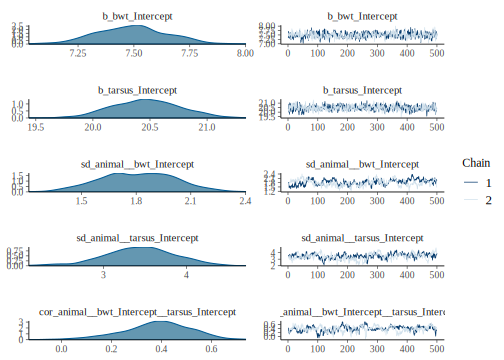
\includegraphics{wam_tuto_files/figure-latex/unnamed-chunk-145-1.pdf} 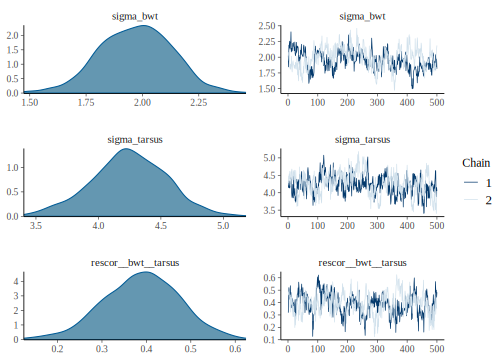
\includegraphics{wam_tuto_files/figure-latex/unnamed-chunk-145-2.pdf}

\begin{Shaded}
\begin{Highlighting}[]
\KeywordTok{VarCorr}\NormalTok{(brms\_m2}\FloatTok{.1}\NormalTok{)}
\end{Highlighting}
\end{Shaded}

\begin{verbatim}
## $animal
## $animal$sd
##                  Estimate Est.Error     Q2.5    Q97.5
## bwt_Intercept    1.808171 0.2050233 1.412824 2.204805
## tarsus_Intercept 3.438368 0.4283612 2.491218 4.245264
## 
## $animal$cor
## , , bwt_Intercept
## 
##                   Estimate Est.Error       Q2.5     Q97.5
## bwt_Intercept    1.0000000 0.0000000 1.00000000 1.0000000
## tarsus_Intercept 0.3814062 0.1380014 0.07581464 0.6209038
## 
## , , tarsus_Intercept
## 
##                   Estimate Est.Error       Q2.5     Q97.5
## bwt_Intercept    0.3814062 0.1380014 0.07581464 0.6209038
## tarsus_Intercept 1.0000000 0.0000000 1.00000000 1.0000000
## 
## 
## $animal$cov
## , , bwt_Intercept
## 
##                  Estimate Est.Error      Q2.5    Q97.5
## bwt_Intercept    3.311473 0.7430185 1.9960721 4.861167
## tarsus_Intercept 2.440166 1.0901689 0.3870783 4.668720
## 
## , , tarsus_Intercept
## 
##                   Estimate Est.Error      Q2.5    Q97.5
## bwt_Intercept     2.440166  1.090169 0.3870783  4.66872
## tarsus_Intercept 12.005688  2.918741 6.2061701 18.02226
## 
## 
## 
## $residual__
## $residual__$sd
##        Estimate Est.Error     Q2.5    Q97.5
## bwt    1.970532 0.1597581 1.658782 2.276074
## tarsus 4.244704 0.2984518 3.632824 4.820109
## 
## $residual__$cor
## , , bwt
## 
##         Estimate  Est.Error      Q2.5     Q97.5
## bwt    1.0000000 0.00000000 1.0000000 1.0000000
## tarsus 0.3888754 0.08510488 0.2127907 0.5526631
## 
## , , tarsus
## 
##         Estimate  Est.Error      Q2.5     Q97.5
## bwt    0.3888754 0.08510488 0.2127907 0.5526631
## tarsus 1.0000000 0.00000000 1.0000000 1.0000000
## 
## 
## $residual__$cov
## , , bwt
## 
##        Estimate Est.Error     Q2.5    Q97.5
## bwt    3.908493 0.6282892 2.751557 5.180511
## tarsus 3.289995 0.9305960 1.572647 5.147133
## 
## , , tarsus
## 
##         Estimate Est.Error      Q2.5     Q97.5
## bwt     3.289995  0.930596  1.572647  5.147133
## tarsus 18.106495  2.530138 13.197409 23.233452
\end{verbatim}

It is also possible to calculate the heritability for each trait using the function `as.mcmc'

\begin{Shaded}
\begin{Highlighting}[]
\NormalTok{v\_animal \textless{}{-}}\StringTok{ }\NormalTok{(}\KeywordTok{VarCorr}\NormalTok{(brms\_m2}\FloatTok{.1}\NormalTok{, }\DataTypeTok{summary =} \OtherTok{FALSE}\NormalTok{)}\OperatorTok{$}\NormalTok{animal}\OperatorTok{$}\NormalTok{sd)}\OperatorTok{\^{}}\DecValTok{2}
\NormalTok{v\_r \textless{}{-}}\StringTok{ }\NormalTok{(}\KeywordTok{VarCorr}\NormalTok{(brms\_m2}\FloatTok{.1}\NormalTok{, }\DataTypeTok{summary =} \OtherTok{FALSE}\NormalTok{)}\OperatorTok{$}\NormalTok{residual}\OperatorTok{$}\NormalTok{sd)}\OperatorTok{\^{}}\DecValTok{2}

\NormalTok{h.bwt}\FloatTok{.2}\NormalTok{ \textless{}{-}}\StringTok{ }\KeywordTok{as.mcmc}\NormalTok{(v\_animal[, }\DecValTok{1}\NormalTok{] }\OperatorTok{/}\StringTok{ }\NormalTok{(v\_animal[, }\DecValTok{1}\NormalTok{] }\OperatorTok{+}\StringTok{ }\NormalTok{v\_r[, }\DecValTok{1}\NormalTok{]))}
\NormalTok{h.tarsus}\FloatTok{.2}\NormalTok{ \textless{}{-}}\StringTok{ }\KeywordTok{as.mcmc}\NormalTok{(v\_animal[, }\DecValTok{1}\NormalTok{] }\OperatorTok{/}\StringTok{ }\NormalTok{(v\_animal[, }\DecValTok{1}\NormalTok{] }\OperatorTok{+}\StringTok{ }\NormalTok{v\_r[, }\DecValTok{1}\NormalTok{]))}

\KeywordTok{summary}\NormalTok{(h.bwt}\FloatTok{.2}\NormalTok{)}
\end{Highlighting}
\end{Shaded}

\begin{verbatim}
## 
## Iterations = 1:1000
## Thinning interval = 1 
## Number of chains = 1 
## Sample size per chain = 1000 
## 
## 1. Empirical mean and standard deviation for each variable,
##    plus standard error of the mean:
## 
##           Mean             SD       Naive SE Time-series SE 
##       0.457051       0.090878       0.002874       0.011675 
## 
## 2. Quantiles for each variable:
## 
##   2.5%    25%    50%    75%  97.5% 
## 0.2878 0.3926 0.4596 0.5254 0.6297
\end{verbatim}

\begin{Shaded}
\begin{Highlighting}[]
\KeywordTok{summary}\NormalTok{(h.tarsus}\FloatTok{.2}\NormalTok{)}
\end{Highlighting}
\end{Shaded}

\begin{verbatim}
## 
## Iterations = 1:1000
## Thinning interval = 1 
## Number of chains = 1 
## Sample size per chain = 1000 
## 
## 1. Empirical mean and standard deviation for each variable,
##    plus standard error of the mean:
## 
##           Mean             SD       Naive SE Time-series SE 
##       0.457051       0.090878       0.002874       0.011675 
## 
## 2. Quantiles for each variable:
## 
##   2.5%    25%    50%    75%  97.5% 
## 0.2878 0.3926 0.4596 0.5254 0.6297
\end{verbatim}

\begin{Shaded}
\begin{Highlighting}[]
\KeywordTok{plot}\NormalTok{(h.bwt}\FloatTok{.2}\NormalTok{)}
\KeywordTok{plot}\NormalTok{(h.tarsus}\FloatTok{.2}\NormalTok{)}
\end{Highlighting}
\end{Shaded}

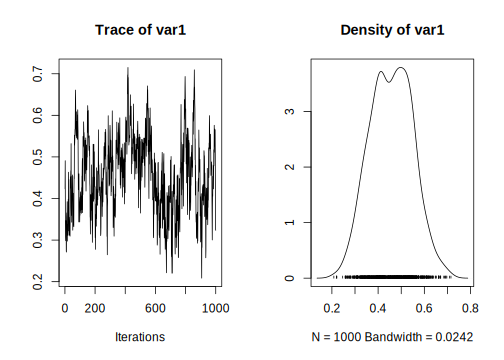
\includegraphics{wam_tuto_files/figure-latex/unnamed-chunk-146-1.pdf}

It is also possible to extract the correlation. Just to remember it is an example, the correlation distribution is skewed to 1 due to a weak prior and model parameters.
Note, since

\begin{Shaded}
\begin{Highlighting}[]
\NormalTok{cor\_g \textless{}{-}}\StringTok{ }\KeywordTok{as.mcmc}\NormalTok{((}\KeywordTok{VarCorr}\NormalTok{(brms\_m2}\FloatTok{.1}\NormalTok{, }\DataTypeTok{summary =} \OtherTok{FALSE}\NormalTok{)}\OperatorTok{$}\NormalTok{animal}\OperatorTok{$}\NormalTok{cor[, }\DecValTok{1}\NormalTok{, }\DecValTok{2}\NormalTok{]))}
\NormalTok{cor\_res \textless{}{-}}\StringTok{ }\KeywordTok{as.mcmc}\NormalTok{((}\KeywordTok{VarCorr}\NormalTok{(brms\_m2}\FloatTok{.1}\NormalTok{, }\DataTypeTok{summary =} \OtherTok{FALSE}\NormalTok{)}\OperatorTok{$}\NormalTok{residual}\OperatorTok{$}\NormalTok{cor[, }\DecValTok{1}\NormalTok{, }\DecValTok{2}\NormalTok{]))}

\KeywordTok{summary}\NormalTok{(cor\_g)}
\end{Highlighting}
\end{Shaded}

\begin{verbatim}
## 
## Iterations = 1:1000
## Thinning interval = 1 
## Number of chains = 1 
## Sample size per chain = 1000 
## 
## 1. Empirical mean and standard deviation for each variable,
##    plus standard error of the mean:
## 
##           Mean             SD       Naive SE Time-series SE 
##       0.381406       0.138001       0.004364       0.014946 
## 
## 2. Quantiles for each variable:
## 
##    2.5%     25%     50%     75%   97.5% 
## 0.07581 0.30354 0.39041 0.47497 0.62090
\end{verbatim}

\begin{Shaded}
\begin{Highlighting}[]
\KeywordTok{summary}\NormalTok{(cor\_res)}
\end{Highlighting}
\end{Shaded}

\begin{verbatim}
## 
## Iterations = 1:1000
## Thinning interval = 1 
## Number of chains = 1 
## Sample size per chain = 1000 
## 
## 1. Empirical mean and standard deviation for each variable,
##    plus standard error of the mean:
## 
##           Mean             SD       Naive SE Time-series SE 
##       0.388875       0.085105       0.002691       0.009215 
## 
## 2. Quantiles for each variable:
## 
##   2.5%    25%    50%    75%  97.5% 
## 0.2128 0.3319 0.3913 0.4484 0.5527
\end{verbatim}

\begin{Shaded}
\begin{Highlighting}[]
\KeywordTok{plot}\NormalTok{(cor\_g)}
\end{Highlighting}
\end{Shaded}

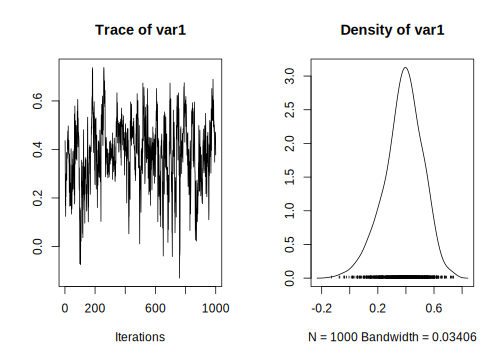
\includegraphics{wam_tuto_files/figure-latex/unnamed-chunk-147-1.pdf}

\begin{Shaded}
\begin{Highlighting}[]
\KeywordTok{plot}\NormalTok{(cor\_res)}
\end{Highlighting}
\end{Shaded}

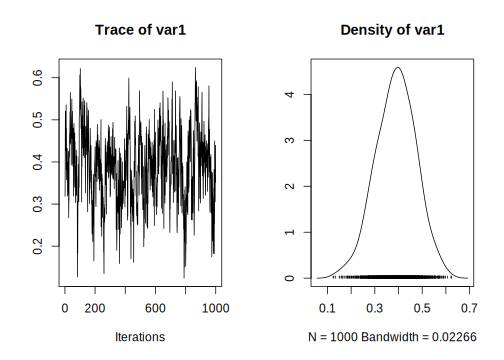
\includegraphics{wam_tuto_files/figure-latex/unnamed-chunk-147-2.pdf}

Here we can plot the genetic correlation by extraction the breeding values or BLUP.

\begin{Shaded}
\begin{Highlighting}[]
\NormalTok{bls\_m2}\FloatTok{.1}\NormalTok{ \textless{}{-}}\StringTok{ }\KeywordTok{ranef}\NormalTok{(brms\_m2}\FloatTok{.1}\NormalTok{)}\OperatorTok{$}\NormalTok{animal}
\NormalTok{bl\_m2}\FloatTok{.1}\NormalTok{ \textless{}{-}}\StringTok{ }\KeywordTok{as.data.frame}\NormalTok{(abind}\OperatorTok{::}\KeywordTok{abind}\NormalTok{(}\KeywordTok{lapply}\NormalTok{(}\DecValTok{1}\OperatorTok{:}\KeywordTok{dim}\NormalTok{(bls\_m2}\FloatTok{.1}\NormalTok{)[[}\DecValTok{3}\NormalTok{]], }\ControlFlowTok{function}\NormalTok{(x) bls\_m2}\FloatTok{.1}\NormalTok{[, }\KeywordTok{c}\NormalTok{(}\DecValTok{1}\NormalTok{, }\DecValTok{3}\NormalTok{, }\DecValTok{4}\NormalTok{), x])))}
\KeywordTok{colnames}\NormalTok{(bl\_m2}\FloatTok{.1}\NormalTok{) \textless{}{-}}\StringTok{ }\KeywordTok{paste0}\NormalTok{(}\KeywordTok{rep}\NormalTok{(}\KeywordTok{dimnames}\NormalTok{(bls\_m2}\FloatTok{.1}\NormalTok{)[[}\DecValTok{3}\NormalTok{]], }\DataTypeTok{each =} \DecValTok{3}\NormalTok{), }\KeywordTok{c}\NormalTok{(}\StringTok{""}\NormalTok{, }\StringTok{"\_lo"}\NormalTok{, }\StringTok{"\_up"}\NormalTok{))}
\NormalTok{bl\_m2}\FloatTok{.1}\OperatorTok{$}\NormalTok{id \textless{}{-}}\StringTok{ }\KeywordTok{rownames}\NormalTok{(bl\_m2}\FloatTok{.1}\NormalTok{)}
\end{Highlighting}
\end{Shaded}

Here, some simple code to plot the genetic correlation.

\begin{Shaded}
\begin{Highlighting}[]
\KeywordTok{plot}\NormalTok{(tarsus\_Intercept }\OperatorTok{\textasciitilde{}}\StringTok{ }\NormalTok{bwt\_Intercept, bl\_m2}\FloatTok{.1}\NormalTok{,}
  \DataTypeTok{xlab =} \StringTok{""}\NormalTok{, }\DataTypeTok{ylab =} \StringTok{""}\NormalTok{,}
  \DataTypeTok{xlim =} \KeywordTok{c}\NormalTok{(}\KeywordTok{min}\NormalTok{(bl\_m2}\FloatTok{.1}\OperatorTok{$}\NormalTok{bwt\_Intercept\_lo), }\KeywordTok{max}\NormalTok{(bl\_m2}\FloatTok{.1}\OperatorTok{$}\NormalTok{bwt\_Intercept\_up)),}
  \DataTypeTok{ylim =} \KeywordTok{c}\NormalTok{(}\KeywordTok{min}\NormalTok{(bl\_m2}\FloatTok{.1}\OperatorTok{$}\NormalTok{tarsus\_Intercept\_lo), }\KeywordTok{max}\NormalTok{(bl\_m2}\FloatTok{.1}\OperatorTok{$}\NormalTok{tarsus\_Intercept\_up)),}
  \DataTypeTok{las =} \FloatTok{1.2}\NormalTok{, }\DataTypeTok{type =} \StringTok{"n"}
\NormalTok{)}
\KeywordTok{with}\NormalTok{(}
\NormalTok{  bl\_m2}\FloatTok{.1}\NormalTok{,}
  \KeywordTok{segments}\NormalTok{(}
    \DataTypeTok{x0 =}\NormalTok{ bwt\_Intercept, }\DataTypeTok{y0 =}\NormalTok{ tarsus\_Intercept\_lo,}
    \DataTypeTok{x1 =}\NormalTok{ bwt\_Intercept, }\DataTypeTok{y1 =}\NormalTok{ tarsus\_Intercept\_up,}
    \DataTypeTok{col =} \StringTok{"black"}
\NormalTok{  )}
\NormalTok{)}
\KeywordTok{with}\NormalTok{(bl\_m2}\FloatTok{.1}\NormalTok{, }\KeywordTok{segments}\NormalTok{(}
  \DataTypeTok{x0 =}\NormalTok{ bwt\_Intercept\_lo, }\DataTypeTok{y0 =}\NormalTok{ tarsus\_Intercept,}
  \DataTypeTok{x1 =}\NormalTok{ bwt\_Intercept\_up, }\DataTypeTok{y1 =}\NormalTok{ tarsus\_Intercept,}
  \DataTypeTok{col =} \StringTok{"black"}
\NormalTok{))}
\KeywordTok{points}\NormalTok{(tarsus\_Intercept }\OperatorTok{\textasciitilde{}}\StringTok{ }\NormalTok{bwt\_Intercept, bl\_m2}\FloatTok{.1}\NormalTok{, }\DataTypeTok{pch =} \DecValTok{16}\NormalTok{, }\DataTypeTok{col =} \StringTok{"red"}\NormalTok{, }\DataTypeTok{cex =} \FloatTok{1.5}\NormalTok{)}
\KeywordTok{points}\NormalTok{(tarsus\_Intercept }\OperatorTok{\textasciitilde{}}\StringTok{ }\NormalTok{bwt\_Intercept, bl\_m2}\FloatTok{.1}\NormalTok{, }\DataTypeTok{pch =} \DecValTok{1}\NormalTok{, }\DataTypeTok{col =} \KeywordTok{rgb}\NormalTok{(}\DecValTok{0}\NormalTok{, }\DecValTok{0}\NormalTok{, }\DecValTok{0}\NormalTok{, }\FloatTok{0.3}\NormalTok{), }\DataTypeTok{cex =} \KeywordTok{c}\NormalTok{(}\FloatTok{1.5}\NormalTok{))}
\KeywordTok{mtext}\NormalTok{(}\StringTok{"btw (BV±CI)"}\NormalTok{, }\DataTypeTok{side =} \DecValTok{1}\NormalTok{, }\DataTypeTok{line =} \FloatTok{2.4}\NormalTok{)}
\KeywordTok{mtext}\NormalTok{(}\StringTok{"tarsus (BV±CI)"}\NormalTok{, }\DataTypeTok{side =} \DecValTok{2}\NormalTok{, }\DataTypeTok{line =} \DecValTok{2}\NormalTok{, }\DataTypeTok{las =} \DecValTok{3}\NormalTok{)}
\end{Highlighting}
\end{Shaded}

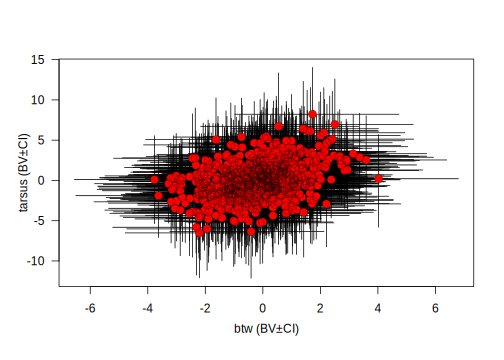
\includegraphics{wam_tuto_files/figure-latex/unnamed-chunk-149-1.pdf}

\hypertarget{adding-fixed-and-random-effects-2}{%
\subsection{Adding fixed and random effects}\label{adding-fixed-and-random-effects-2}}

Fixed and random effects can be added just as for the univariate case.
Given that our full model of bwt from tutorial 1 had sex as a fixed effect as well as random effects of byear and mother, we could specify a bivariate formulation of this using the following code (including a line to save the output):

\begin{Shaded}
\begin{Highlighting}[]
\NormalTok{bf\_bwt\_}\DecValTok{2}\NormalTok{ \textless{}{-}}\StringTok{ }\KeywordTok{bf}\NormalTok{(bwt }\OperatorTok{\textasciitilde{}}\StringTok{ }\DecValTok{1} \OperatorTok{+}\StringTok{ }\NormalTok{sex }\OperatorTok{+}\StringTok{ }\NormalTok{(}\DecValTok{1} \OperatorTok{|}\StringTok{ }\NormalTok{a }\OperatorTok{|}\StringTok{ }\KeywordTok{gr}\NormalTok{(animal, }\DataTypeTok{cov =}\NormalTok{ Amat)) }\OperatorTok{+}\StringTok{ }\NormalTok{(}\DecValTok{1} \OperatorTok{|}\StringTok{ }\NormalTok{b }\OperatorTok{|}\StringTok{ }\NormalTok{byear) }\OperatorTok{+}\StringTok{ }\NormalTok{(}\DecValTok{1} \OperatorTok{|}\StringTok{ }\NormalTok{c }\OperatorTok{|}\StringTok{ }\NormalTok{mother))}
\NormalTok{bf\_tarsus\_}\DecValTok{2}\NormalTok{ \textless{}{-}}\StringTok{ }\KeywordTok{bf}\NormalTok{(tarsus }\OperatorTok{\textasciitilde{}}\StringTok{ }\DecValTok{1} \OperatorTok{+}\StringTok{ }\NormalTok{sex }\OperatorTok{+}\StringTok{ }\NormalTok{(}\DecValTok{1} \OperatorTok{|}\StringTok{ }\NormalTok{a }\OperatorTok{|}\StringTok{ }\KeywordTok{gr}\NormalTok{(animal, }\DataTypeTok{cov =}\NormalTok{ Amat)) }\OperatorTok{+}\StringTok{ }\NormalTok{(}\DecValTok{1} \OperatorTok{|}\StringTok{ }\NormalTok{b }\OperatorTok{|}\StringTok{ }\NormalTok{byear) }\OperatorTok{+}\StringTok{ }\NormalTok{(}\DecValTok{1} \OperatorTok{|}\StringTok{ }\NormalTok{c }\OperatorTok{|}\StringTok{ }\NormalTok{mother))}

\NormalTok{brms\_m2}\FloatTok{.2}\NormalTok{ \textless{}{-}}\StringTok{ }\KeywordTok{brm}\NormalTok{(}
\NormalTok{  bf\_bwt\_}\DecValTok{2} \OperatorTok{+}\StringTok{ }\NormalTok{bf\_tarsus\_}\DecValTok{2} \OperatorTok{+}\StringTok{ }\KeywordTok{set\_rescor}\NormalTok{(}\OtherTok{TRUE}\NormalTok{),}
  \DataTypeTok{data =}\NormalTok{ gryphon,}
  \DataTypeTok{data2 =} \KeywordTok{list}\NormalTok{(}\DataTypeTok{Amat =}\NormalTok{ Amat),}
  \DataTypeTok{chains =} \DecValTok{2}\NormalTok{, }\DataTypeTok{cores =} \DecValTok{2}\NormalTok{, }\DataTypeTok{iter =} \DecValTok{1000}
\NormalTok{)}

\KeywordTok{save}\NormalTok{(brms\_m2}\FloatTok{.2}\NormalTok{, }\DataTypeTok{file =} \StringTok{"data/brms\_m2\_2.rda"}\NormalTok{)}
\end{Highlighting}
\end{Shaded}

Again we have provided the data from one such run. It can be accessed using the code:

\begin{Shaded}
\begin{Highlighting}[]
\KeywordTok{load}\NormalTok{(}\StringTok{"data/brms\_m2\_2.rda"}\NormalTok{)}
\KeywordTok{summary}\NormalTok{(brms\_m2}\FloatTok{.2}\NormalTok{)}
\end{Highlighting}
\end{Shaded}

\begin{verbatim}
## Warning: Parts of the model have not converged (some Rhats are > 1.05). Be
## careful when analysing the results! We recommend running more iterations and/or
## setting stronger priors.
\end{verbatim}

\begin{verbatim}
## Warning: There were 4 divergent transitions after warmup. Increasing adapt_delta
## above 0.8 may help. See http://mc-stan.org/misc/warnings.html#divergent-
## transitions-after-warmup
\end{verbatim}

\begin{verbatim}
##  Family: MV(gaussian, gaussian) 
##   Links: mu = identity; sigma = identity
##          mu = identity; sigma = identity 
## Formula: bwt ~ 1 + sex + (1 | a | gr(animal, cov = Amat)) + (1 | b | byear) + (1 | c | mother) 
##          tarsus ~ 1 + sex + (1 | a | gr(animal, cov = Amat)) + (1 | b | byear) + (1 | c | mother) 
##    Data: gryphon (Number of observations: 683) 
##   Draws: 2 chains, each with iter = 1000; warmup = 500; thin = 1;
##          total post-warmup draws = 1000
## 
## Group-Level Effects: 
## ~animal (Number of levels: 683) 
##                                     Estimate Est.Error l-95% CI u-95% CI Rhat
## sd(bwt_Intercept)                       1.31      0.21     0.86     1.69 1.06
## sd(tarsus_Intercept)                    2.88      0.47     1.88     3.70 1.01
## cor(bwt_Intercept,tarsus_Intercept)     0.60      0.17     0.18     0.89 1.09
##                                     Bulk_ESS Tail_ESS
## sd(bwt_Intercept)                         54       58
## sd(tarsus_Intercept)                      52      162
## cor(bwt_Intercept,tarsus_Intercept)       25       30
## 
## ~byear (Number of levels: 34) 
##                                     Estimate Est.Error l-95% CI u-95% CI Rhat
## sd(bwt_Intercept)                       0.99      0.17     0.71     1.39 1.00
## sd(tarsus_Intercept)                    2.02      0.34     1.45     2.78 1.00
## cor(bwt_Intercept,tarsus_Intercept)     0.01      0.22    -0.44     0.44 1.01
##                                     Bulk_ESS Tail_ESS
## sd(bwt_Intercept)                        424      509
## sd(tarsus_Intercept)                     525      699
## cor(bwt_Intercept,tarsus_Intercept)      478      492
## 
## ~mother (Number of levels: 352) 
##                                     Estimate Est.Error l-95% CI u-95% CI Rhat
## sd(bwt_Intercept)                       1.14      0.12     0.90     1.36 1.01
## sd(tarsus_Intercept)                    2.09      0.29     1.54     2.67 1.01
## cor(bwt_Intercept,tarsus_Intercept)    -0.64      0.20    -0.97    -0.24 1.02
##                                     Bulk_ESS Tail_ESS
## sd(bwt_Intercept)                        370      764
## sd(tarsus_Intercept)                     134      420
## cor(bwt_Intercept,tarsus_Intercept)       84      147
## 
## Population-Level Effects: 
##                  Estimate Est.Error l-95% CI u-95% CI Rhat Bulk_ESS Tail_ESS
## bwt_Intercept        6.28      0.24     5.80     6.73 1.00      453      703
## tarsus_Intercept    20.39      0.52    19.45    21.39 1.00      755      760
## bwt_sex2             2.05      0.17     1.71     2.37 1.00     1097      715
## tarsus_sex2          0.11      0.42    -0.67     0.90 1.00      780      578
## 
## Family Specific Parameters: 
##              Estimate Est.Error l-95% CI u-95% CI Rhat Bulk_ESS Tail_ESS
## sigma_bwt        1.40      0.16     1.05     1.68 1.04       59       60
## sigma_tarsus     3.73      0.32     3.14     4.32 1.00       55      176
## 
## Residual Correlations: 
##                    Estimate Est.Error l-95% CI u-95% CI Rhat Bulk_ESS Tail_ESS
## rescor(bwt,tarsus)     0.89      0.07     0.72     0.98 1.50        4       24
## 
## Draws were sampled using sampling(NUTS). For each parameter, Bulk_ESS
## and Tail_ESS are effective sample size measures, and Rhat is the potential
## scale reduction factor on split chains (at convergence, Rhat = 1).
\end{verbatim}

\begin{Shaded}
\begin{Highlighting}[]
\KeywordTok{plot}\NormalTok{(brms\_m2}\FloatTok{.2}\NormalTok{, }\DataTypeTok{ask =} \OtherTok{FALSE}\NormalTok{)}
\end{Highlighting}
\end{Shaded}

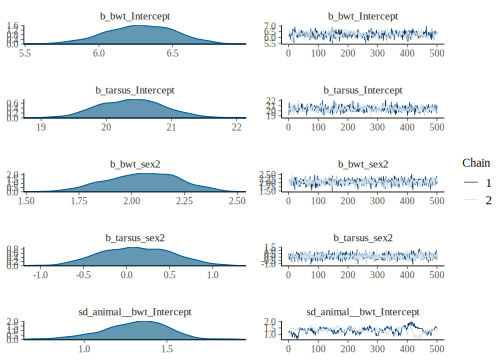
\includegraphics{wam_tuto_files/figure-latex/unnamed-chunk-151-1.pdf} 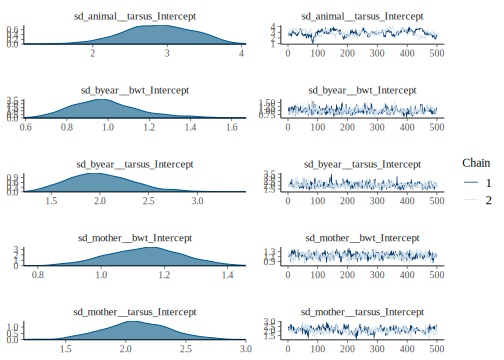
\includegraphics{wam_tuto_files/figure-latex/unnamed-chunk-151-2.pdf} 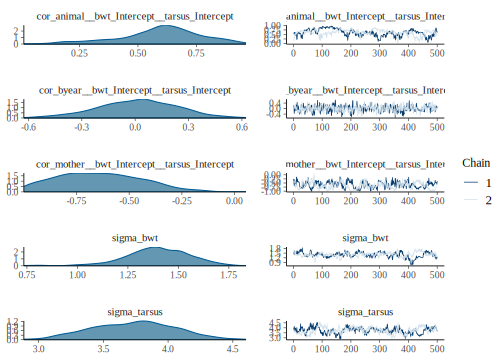
\includegraphics{wam_tuto_files/figure-latex/unnamed-chunk-151-3.pdf} 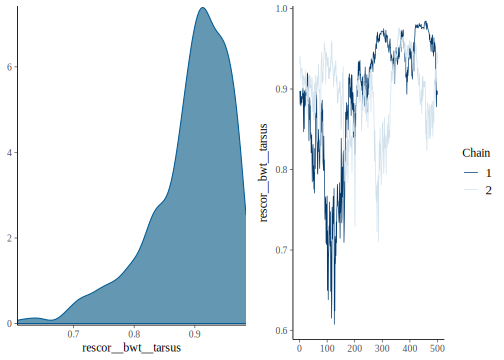
\includegraphics{wam_tuto_files/figure-latex/unnamed-chunk-151-4.pdf}

\begin{Shaded}
\begin{Highlighting}[]
\KeywordTok{VarCorr}\NormalTok{(brms\_m2}\FloatTok{.2}\NormalTok{)}
\end{Highlighting}
\end{Shaded}

\begin{verbatim}
## $animal
## $animal$sd
##                  Estimate Est.Error      Q2.5    Q97.5
## bwt_Intercept    1.306921 0.2109780 0.8555702 1.687254
## tarsus_Intercept 2.876731 0.4718524 1.8827128 3.699873
## 
## $animal$cor
## , , bwt_Intercept
## 
##                   Estimate Est.Error      Q2.5     Q97.5
## bwt_Intercept    1.0000000 0.0000000 1.0000000 1.0000000
## tarsus_Intercept 0.5961514 0.1727943 0.1849725 0.8929607
## 
## , , tarsus_Intercept
## 
##                   Estimate Est.Error      Q2.5     Q97.5
## bwt_Intercept    0.5961514 0.1727943 0.1849725 0.8929607
## tarsus_Intercept 1.0000000 0.0000000 1.0000000 1.0000000
## 
## 
## $animal$cov
## , , bwt_Intercept
## 
##                  Estimate Est.Error      Q2.5    Q97.5
## bwt_Intercept    1.752510 0.5433004 0.7320013 2.846827
## tarsus_Intercept 2.357852 1.0462644 0.3960956 4.526731
## 
## , , tarsus_Intercept
## 
##                  Estimate Est.Error      Q2.5     Q97.5
## bwt_Intercept    2.357852  1.046264 0.3960956  4.526731
## tarsus_Intercept 8.498003  2.672465 3.5446115 13.689062
## 
## 
## 
## $byear
## $byear$sd
##                   Estimate Est.Error      Q2.5    Q97.5
## bwt_Intercept    0.9904858 0.1696752 0.7102391 1.390260
## tarsus_Intercept 2.0166804 0.3366954 1.4463862 2.777005
## 
## $byear$cor
## , , bwt_Intercept
## 
##                    Estimate Est.Error       Q2.5     Q97.5
## bwt_Intercept    1.00000000 0.0000000  1.0000000 1.0000000
## tarsus_Intercept 0.01351405 0.2206186 -0.4367809 0.4412319
## 
## , , tarsus_Intercept
## 
##                    Estimate Est.Error       Q2.5     Q97.5
## bwt_Intercept    0.01351405 0.2206186 -0.4367809 0.4412319
## tarsus_Intercept 1.00000000 0.0000000  1.0000000 1.0000000
## 
## 
## $byear$cov
## , , bwt_Intercept
## 
##                    Estimate Est.Error       Q2.5    Q97.5
## bwt_Intercept    1.00982294 0.3583697  0.5044397 1.932823
## tarsus_Intercept 0.06412895 0.4880116 -0.8559486 1.092317
## 
## , , tarsus_Intercept
## 
##                    Estimate Est.Error       Q2.5    Q97.5
## bwt_Intercept    0.06412895 0.4880116 -0.8559486 1.092317
## tarsus_Intercept 4.18025049 1.4249595  2.0920330 7.711755
## 
## 
## 
## $mother
## $mother$sd
##                  Estimate Est.Error      Q2.5    Q97.5
## bwt_Intercept    1.137249 0.1175495 0.8968349 1.358078
## tarsus_Intercept 2.088602 0.2865291 1.5425683 2.673791
## 
## $mother$cor
## , , bwt_Intercept
## 
##                    Estimate Est.Error       Q2.5      Q97.5
## bwt_Intercept     1.0000000 0.0000000  1.0000000  1.0000000
## tarsus_Intercept -0.6413329 0.1968102 -0.9745925 -0.2367393
## 
## , , tarsus_Intercept
## 
##                    Estimate Est.Error       Q2.5      Q97.5
## bwt_Intercept    -0.6413329 0.1968102 -0.9745925 -0.2367393
## tarsus_Intercept  1.0000000 0.0000000  1.0000000  1.0000000
## 
## 
## $mother$cov
## , , bwt_Intercept
## 
##                   Estimate Est.Error       Q2.5      Q97.5
## bwt_Intercept     1.307139 0.2669748  0.8043132  1.8443762
## tarsus_Intercept -1.467511 0.3650113 -2.1491979 -0.6718737
## 
## , , tarsus_Intercept
## 
##                   Estimate Est.Error      Q2.5      Q97.5
## bwt_Intercept    -1.467511 0.3650113 -2.149198 -0.6718737
## tarsus_Intercept  4.444274 1.2018090  2.379517  7.1491575
## 
## 
## 
## $residual__
## $residual__$sd
##        Estimate Est.Error     Q2.5    Q97.5
## bwt    1.396815 0.1597393 1.052042 1.684810
## tarsus 3.733614 0.3170549 3.140204 4.319446
## 
## $residual__$cor
## , , bwt
## 
##         Estimate Est.Error      Q2.5     Q97.5
## bwt    1.0000000 0.0000000 1.0000000 1.0000000
## tarsus 0.8925119 0.0672286 0.7167862 0.9774545
## 
## , , tarsus
## 
##         Estimate Est.Error      Q2.5     Q97.5
## bwt    0.8925119 0.0672286 0.7167862 0.9774545
## tarsus 1.0000000 0.0000000 1.0000000 1.0000000
## 
## 
## $residual__$cov
## , , bwt
## 
##        Estimate Est.Error     Q2.5    Q97.5
## bwt    1.976584 0.4347085 1.106793 2.838585
## tarsus 4.683451 0.9103808 2.846560 6.440550
## 
## , , tarsus
## 
##         Estimate Est.Error     Q2.5    Q97.5
## bwt     4.683451 0.9103808 2.846560  6.44055
## tarsus 14.040300 2.3674563 9.860883 18.65761
\end{verbatim}

Evaluation of the statistical support for these genetic and maternal correlations is straightforward. Because we imposed no constraint on their estimation, we can evaluate the extent to which the posterior distributions overlap zero:

\begin{Shaded}
\begin{Highlighting}[]
\NormalTok{cor\_g \textless{}{-}}\StringTok{ }\KeywordTok{as.mcmc}\NormalTok{((}\KeywordTok{VarCorr}\NormalTok{(brms\_m2}\FloatTok{.2}\NormalTok{, }\DataTypeTok{summary =} \OtherTok{FALSE}\NormalTok{)}\OperatorTok{$}\NormalTok{animal}\OperatorTok{$}\NormalTok{cor[, }\DecValTok{1}\NormalTok{, }\DecValTok{2}\NormalTok{]))}
\NormalTok{cor\_res \textless{}{-}}\StringTok{ }\KeywordTok{as.mcmc}\NormalTok{((}\KeywordTok{VarCorr}\NormalTok{(brms\_m2}\FloatTok{.2}\NormalTok{, }\DataTypeTok{summary =} \OtherTok{FALSE}\NormalTok{)}\OperatorTok{$}\NormalTok{residual}\OperatorTok{$}\NormalTok{cor[, }\DecValTok{1}\NormalTok{, }\DecValTok{2}\NormalTok{]))}
\NormalTok{cor\_mother \textless{}{-}}\StringTok{ }\KeywordTok{as.mcmc}\NormalTok{((}\KeywordTok{VarCorr}\NormalTok{(brms\_m2}\FloatTok{.2}\NormalTok{, }\DataTypeTok{summary =} \OtherTok{FALSE}\NormalTok{)}\OperatorTok{$}\NormalTok{mother}\OperatorTok{$}\NormalTok{cor[, }\DecValTok{1}\NormalTok{, }\DecValTok{2}\NormalTok{]))}
\NormalTok{cor\_byear \textless{}{-}}\StringTok{ }\KeywordTok{as.mcmc}\NormalTok{((}\KeywordTok{VarCorr}\NormalTok{(brms\_m2}\FloatTok{.2}\NormalTok{, }\DataTypeTok{summary =} \OtherTok{FALSE}\NormalTok{)}\OperatorTok{$}\NormalTok{byear}\OperatorTok{$}\NormalTok{cor[, }\DecValTok{1}\NormalTok{, }\DecValTok{2}\NormalTok{]))}

\KeywordTok{summary}\NormalTok{(cor\_g)}
\end{Highlighting}
\end{Shaded}

\begin{verbatim}
## 
## Iterations = 1:1000
## Thinning interval = 1 
## Number of chains = 1 
## Sample size per chain = 1000 
## 
## 1. Empirical mean and standard deviation for each variable,
##    plus standard error of the mean:
## 
##           Mean             SD       Naive SE Time-series SE 
##       0.596151       0.172794       0.005464       0.028178 
## 
## 2. Quantiles for each variable:
## 
##   2.5%    25%    50%    75%  97.5% 
## 0.1850 0.5065 0.6117 0.7064 0.8930
\end{verbatim}

\begin{Shaded}
\begin{Highlighting}[]
\KeywordTok{summary}\NormalTok{(cor\_mother)}
\end{Highlighting}
\end{Shaded}

\begin{verbatim}
## 
## Iterations = 1:1000
## Thinning interval = 1 
## Number of chains = 1 
## Sample size per chain = 1000 
## 
## 1. Empirical mean and standard deviation for each variable,
##    plus standard error of the mean:
## 
##           Mean             SD       Naive SE Time-series SE 
##      -0.641333       0.196810       0.006224       0.021355 
## 
## 2. Quantiles for each variable:
## 
##    2.5%     25%     50%     75%   97.5% 
## -0.9746 -0.7933 -0.6507 -0.5027 -0.2367
\end{verbatim}

\begin{Shaded}
\begin{Highlighting}[]
\KeywordTok{summary}\NormalTok{(cor\_byear)}
\end{Highlighting}
\end{Shaded}

\begin{verbatim}
## 
## Iterations = 1:1000
## Thinning interval = 1 
## Number of chains = 1 
## Sample size per chain = 1000 
## 
## 1. Empirical mean and standard deviation for each variable,
##    plus standard error of the mean:
## 
##           Mean             SD       Naive SE Time-series SE 
##       0.013514       0.220619       0.006977       0.009633 
## 
## 2. Quantiles for each variable:
## 
##     2.5%      25%      50%      75%    97.5% 
## -0.43678 -0.13505  0.02408  0.16947  0.44123
\end{verbatim}

\begin{Shaded}
\begin{Highlighting}[]
\KeywordTok{summary}\NormalTok{(cor\_res)}
\end{Highlighting}
\end{Shaded}

\begin{verbatim}
## 
## Iterations = 1:1000
## Thinning interval = 1 
## Number of chains = 1 
## Sample size per chain = 1000 
## 
## 1. Empirical mean and standard deviation for each variable,
##    plus standard error of the mean:
## 
##           Mean             SD       Naive SE Time-series SE 
##       0.892512       0.067229       0.002126       0.026496 
## 
## 2. Quantiles for each variable:
## 
##   2.5%    25%    50%    75%  97.5% 
## 0.7168 0.8620 0.9069 0.9425 0.9775
\end{verbatim}

\begin{Shaded}
\begin{Highlighting}[]
\KeywordTok{plot}\NormalTok{(cor\_g)}
\end{Highlighting}
\end{Shaded}

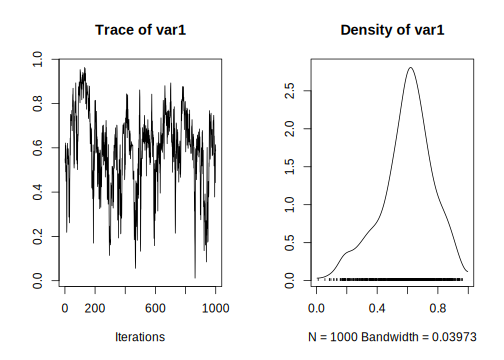
\includegraphics{wam_tuto_files/figure-latex/unnamed-chunk-152-1.pdf}

\begin{Shaded}
\begin{Highlighting}[]
\KeywordTok{plot}\NormalTok{(cor\_res)}
\end{Highlighting}
\end{Shaded}

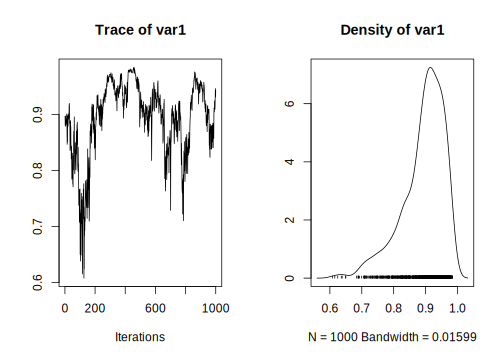
\includegraphics{wam_tuto_files/figure-latex/unnamed-chunk-152-2.pdf}

\begin{Shaded}
\begin{Highlighting}[]
\KeywordTok{plot}\NormalTok{(cor\_mother)}
\end{Highlighting}
\end{Shaded}

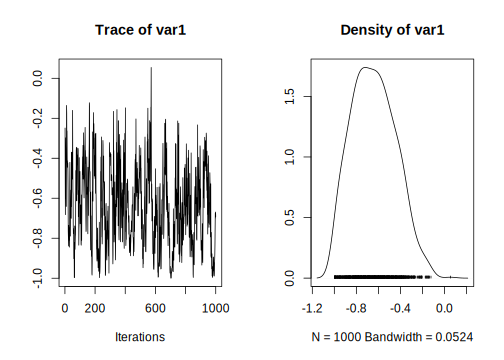
\includegraphics{wam_tuto_files/figure-latex/unnamed-chunk-152-3.pdf}

\begin{Shaded}
\begin{Highlighting}[]
\KeywordTok{plot}\NormalTok{(cor\_byear)}
\end{Highlighting}
\end{Shaded}

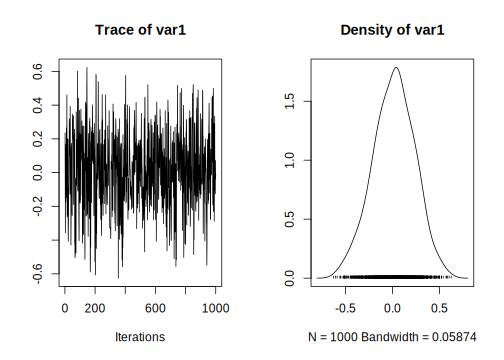
\includegraphics{wam_tuto_files/figure-latex/unnamed-chunk-152-4.pdf}

Neither or these posterior distributions overlaps zero, so we can consider them both statistically supported.

\begin{Shaded}
\begin{Highlighting}[]
\NormalTok{cor.est \textless{}{-}}\StringTok{ }\KeywordTok{rbind}\NormalTok{(}
  \KeywordTok{cbind}\NormalTok{(}\KeywordTok{summary}\NormalTok{(cor\_g)}\OperatorTok{$}\NormalTok{statistics[}\DecValTok{1}\NormalTok{], }\KeywordTok{summary}\NormalTok{(cor\_g)}\OperatorTok{$}\NormalTok{quantiles[}\DecValTok{1}\NormalTok{], }\KeywordTok{summary}\NormalTok{(cor\_g)}\OperatorTok{$}\NormalTok{quantiles[}\DecValTok{5}\NormalTok{]),}
  \KeywordTok{cbind}\NormalTok{(}\KeywordTok{summary}\NormalTok{(cor\_mother)}\OperatorTok{$}\NormalTok{statistics[}\DecValTok{1}\NormalTok{], }\KeywordTok{summary}\NormalTok{(cor\_mother)}\OperatorTok{$}\NormalTok{quantiles[}\DecValTok{1}\NormalTok{], }\KeywordTok{summary}\NormalTok{(cor\_mother)}\OperatorTok{$}\NormalTok{quantiles[}\DecValTok{5}\NormalTok{]),}
  \KeywordTok{cbind}\NormalTok{(}\KeywordTok{summary}\NormalTok{(cor\_byear)}\OperatorTok{$}\NormalTok{statistics[}\DecValTok{1}\NormalTok{], }\KeywordTok{summary}\NormalTok{(cor\_byear)}\OperatorTok{$}\NormalTok{quantiles[}\DecValTok{1}\NormalTok{], }\KeywordTok{summary}\NormalTok{(cor\_byear)}\OperatorTok{$}\NormalTok{quantiles[}\DecValTok{5}\NormalTok{]),}
  \KeywordTok{cbind}\NormalTok{(}\KeywordTok{summary}\NormalTok{(cor\_res)}\OperatorTok{$}\NormalTok{statistics[}\DecValTok{1}\NormalTok{], }\KeywordTok{summary}\NormalTok{(cor\_res)}\OperatorTok{$}\NormalTok{quantiles[}\DecValTok{1}\NormalTok{], }\KeywordTok{summary}\NormalTok{(cor\_res)}\OperatorTok{$}\NormalTok{quantiles[}\DecValTok{5}\NormalTok{])}
\NormalTok{)}


\KeywordTok{plot}\NormalTok{(}\KeywordTok{c}\NormalTok{(}\DecValTok{1}\NormalTok{, }\DecValTok{2}\NormalTok{, }\DecValTok{3}\NormalTok{, }\DecValTok{4}\NormalTok{) }\OperatorTok{\textasciitilde{}}\StringTok{ }\NormalTok{cor.est[, }\DecValTok{1}\NormalTok{], }\DataTypeTok{xlim =} \KeywordTok{c}\NormalTok{(}\OperatorTok{{-}}\DecValTok{1}\NormalTok{, }\DecValTok{1}\NormalTok{), }\DataTypeTok{ylim =} \KeywordTok{c}\NormalTok{(}\DecValTok{0}\NormalTok{, }\DecValTok{5}\NormalTok{), }\DataTypeTok{xlab =} \StringTok{""}\NormalTok{, }\DataTypeTok{ylab =} \StringTok{""}\NormalTok{, }\DataTypeTok{cex =} \DecValTok{2}\NormalTok{, }\DataTypeTok{yaxt =} \StringTok{"n"}\NormalTok{)}
\KeywordTok{segments}\NormalTok{(}\DataTypeTok{y0 =} \DecValTok{1}\NormalTok{, }\DataTypeTok{x0 =}\NormalTok{ cor.est[}\DecValTok{1}\NormalTok{, }\DecValTok{1}\NormalTok{] }\OperatorTok{{-}}\StringTok{ }\NormalTok{cor.est[}\DecValTok{1}\NormalTok{, }\DecValTok{2}\NormalTok{], }\DataTypeTok{y1 =} \DecValTok{1}\NormalTok{, }\DataTypeTok{x1 =}\NormalTok{ cor.est[}\DecValTok{1}\NormalTok{, }\DecValTok{1}\NormalTok{] }\OperatorTok{+}\StringTok{ }\NormalTok{cor.est[}\DecValTok{1}\NormalTok{, }\DecValTok{2}\NormalTok{], }\DataTypeTok{lwd =} \DecValTok{2}\NormalTok{)}
\KeywordTok{segments}\NormalTok{(}\DataTypeTok{y0 =} \DecValTok{2}\NormalTok{, }\DataTypeTok{x0 =}\NormalTok{ cor.est[}\DecValTok{2}\NormalTok{, }\DecValTok{1}\NormalTok{] }\OperatorTok{{-}}\StringTok{ }\NormalTok{cor.est[}\DecValTok{2}\NormalTok{, }\DecValTok{2}\NormalTok{], }\DataTypeTok{y1 =} \DecValTok{2}\NormalTok{, }\DataTypeTok{x1 =}\NormalTok{ cor.est[}\DecValTok{2}\NormalTok{, }\DecValTok{1}\NormalTok{] }\OperatorTok{+}\StringTok{ }\NormalTok{cor.est[}\DecValTok{2}\NormalTok{, }\DecValTok{2}\NormalTok{], }\DataTypeTok{lwd =} \DecValTok{2}\NormalTok{)}
\KeywordTok{segments}\NormalTok{(}\DataTypeTok{y0 =} \DecValTok{3}\NormalTok{, }\DataTypeTok{x0 =}\NormalTok{ cor.est[}\DecValTok{3}\NormalTok{, }\DecValTok{1}\NormalTok{] }\OperatorTok{{-}}\StringTok{ }\NormalTok{cor.est[}\DecValTok{3}\NormalTok{, }\DecValTok{2}\NormalTok{], }\DataTypeTok{y1 =} \DecValTok{3}\NormalTok{, }\DataTypeTok{x1 =}\NormalTok{ cor.est[}\DecValTok{3}\NormalTok{, }\DecValTok{1}\NormalTok{] }\OperatorTok{+}\StringTok{ }\NormalTok{cor.est[}\DecValTok{3}\NormalTok{, }\DecValTok{2}\NormalTok{], }\DataTypeTok{lwd =} \DecValTok{2}\NormalTok{)}
\KeywordTok{segments}\NormalTok{(}\DataTypeTok{y0 =} \DecValTok{4}\NormalTok{, }\DataTypeTok{x0 =}\NormalTok{ cor.est[}\DecValTok{4}\NormalTok{, }\DecValTok{1}\NormalTok{] }\OperatorTok{{-}}\StringTok{ }\NormalTok{cor.est[}\DecValTok{4}\NormalTok{, }\DecValTok{2}\NormalTok{], }\DataTypeTok{y1 =} \DecValTok{4}\NormalTok{, }\DataTypeTok{x1 =}\NormalTok{ cor.est[}\DecValTok{4}\NormalTok{, }\DecValTok{1}\NormalTok{] }\OperatorTok{+}\StringTok{ }\NormalTok{cor.est[}\DecValTok{4}\NormalTok{, }\DecValTok{2}\NormalTok{], }\DataTypeTok{lwd =} \DecValTok{2}\NormalTok{)}
\KeywordTok{mtext}\NormalTok{(}\StringTok{"Correlation (±CI)"}\NormalTok{, }\DataTypeTok{side =} \DecValTok{1}\NormalTok{, }\DataTypeTok{las =} \DecValTok{1}\NormalTok{, }\DataTypeTok{adj =} \FloatTok{0.4}\NormalTok{, }\DataTypeTok{line =} \DecValTok{3}\NormalTok{, }\DataTypeTok{cex =} \FloatTok{1.6}\NormalTok{)}
\KeywordTok{axis}\NormalTok{(}\DecValTok{2}\NormalTok{, }\DataTypeTok{at =} \DecValTok{1}\NormalTok{, }\DataTypeTok{labels =} \KeywordTok{c}\NormalTok{(}\StringTok{"genetic"}\NormalTok{), }\DataTypeTok{las =} \DecValTok{2}\NormalTok{, }\DataTypeTok{cex.axis =} \DecValTok{1}\NormalTok{)}
\KeywordTok{axis}\NormalTok{(}\DecValTok{2}\NormalTok{, }\DataTypeTok{at =} \DecValTok{2}\NormalTok{, }\DataTypeTok{labels =} \KeywordTok{c}\NormalTok{(}\StringTok{"mother"}\NormalTok{), }\DataTypeTok{las =} \DecValTok{2}\NormalTok{, }\DataTypeTok{cex.axis =} \DecValTok{1}\NormalTok{)}
\KeywordTok{axis}\NormalTok{(}\DecValTok{2}\NormalTok{, }\DataTypeTok{at =} \DecValTok{3}\NormalTok{, }\DataTypeTok{labels =} \KeywordTok{c}\NormalTok{(}\StringTok{"year"}\NormalTok{), }\DataTypeTok{las =} \DecValTok{2}\NormalTok{, }\DataTypeTok{cex.axis =} \DecValTok{1}\NormalTok{)}
\KeywordTok{axis}\NormalTok{(}\DecValTok{2}\NormalTok{, }\DataTypeTok{at =} \DecValTok{4}\NormalTok{, }\DataTypeTok{labels =} \KeywordTok{c}\NormalTok{(}\StringTok{"residual"}\NormalTok{), }\DataTypeTok{las =} \DecValTok{2}\NormalTok{, }\DataTypeTok{cex.axis =} \DecValTok{1}\NormalTok{)}
\end{Highlighting}
\end{Shaded}

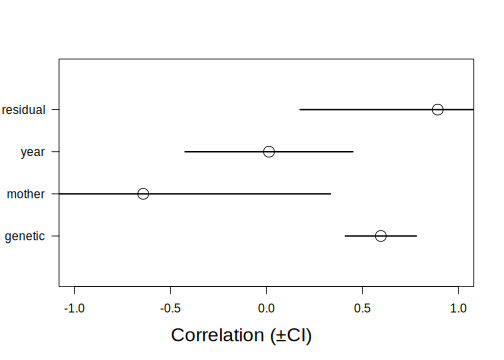
\includegraphics{wam_tuto_files/figure-latex/unnamed-chunk-153-1.pdf}

Note, brms estimates the correlation and also the covariance. We can also recalculate the correlation directly from the covariance.To facilitate the extraction of the different parameter, we can the fucntion \texttt{as\_draws\_df}

\begin{Shaded}
\begin{Highlighting}[]
\NormalTok{cov\_g \textless{}{-}}\StringTok{ }\NormalTok{(}\KeywordTok{VarCorr}\NormalTok{(brms\_m2}\FloatTok{.2}\NormalTok{, }\DataTypeTok{summary =} \OtherTok{FALSE}\NormalTok{)}\OperatorTok{$}\NormalTok{animal}\OperatorTok{$}\NormalTok{cov)[, }\DecValTok{1}\NormalTok{, }\DecValTok{2}\NormalTok{]}
\NormalTok{cov\_res \textless{}{-}}\StringTok{ }\NormalTok{(}\KeywordTok{VarCorr}\NormalTok{(brms\_m2}\FloatTok{.2}\NormalTok{, }\DataTypeTok{summary =} \OtherTok{FALSE}\NormalTok{)}\OperatorTok{$}\NormalTok{residual}\OperatorTok{$}\NormalTok{cov)[, }\DecValTok{1}\NormalTok{, }\DecValTok{2}\NormalTok{]}
\NormalTok{cov\_mother \textless{}{-}}\StringTok{ }\NormalTok{(}\KeywordTok{VarCorr}\NormalTok{(brms\_m2}\FloatTok{.2}\NormalTok{, }\DataTypeTok{summary =} \OtherTok{FALSE}\NormalTok{)}\OperatorTok{$}\NormalTok{mother}\OperatorTok{$}\NormalTok{cov)[, }\DecValTok{1}\NormalTok{, }\DecValTok{2}\NormalTok{]}
\NormalTok{cov\_byear \textless{}{-}}\StringTok{ }\NormalTok{(}\KeywordTok{VarCorr}\NormalTok{(brms\_m2}\FloatTok{.2}\NormalTok{, }\DataTypeTok{summary =} \OtherTok{FALSE}\NormalTok{)}\OperatorTok{$}\NormalTok{byear}\OperatorTok{$}\NormalTok{cov)[, }\DecValTok{1}\NormalTok{, }\DecValTok{2}\NormalTok{]}

\NormalTok{var.est \textless{}{-}}\StringTok{ }\KeywordTok{as\_draws\_df}\NormalTok{(brms\_m2}\FloatTok{.2}\NormalTok{, }\DataTypeTok{variable =} \KeywordTok{c}\NormalTok{(}\StringTok{"sd"}\NormalTok{, }\StringTok{"sigma"}\NormalTok{), }\DataTypeTok{regex =} \OtherTok{TRUE}\NormalTok{)}
\NormalTok{var.est \textless{}{-}}\StringTok{ }\NormalTok{var.est}\OperatorTok{\^{}}\DecValTok{2}

\NormalTok{cor\_g\_}\DecValTok{2}\NormalTok{ \textless{}{-}}\StringTok{ }\KeywordTok{as.mcmc}\NormalTok{(cov\_g }\OperatorTok{/}\StringTok{ }\KeywordTok{sqrt}\NormalTok{(var.est[}\DecValTok{1}\NormalTok{] }\OperatorTok{*}\StringTok{ }\NormalTok{var.est[}\DecValTok{2}\NormalTok{]))}
\NormalTok{cor\_byear\_}\DecValTok{2}\NormalTok{ \textless{}{-}}\StringTok{ }\KeywordTok{as.mcmc}\NormalTok{(cov\_byear }\OperatorTok{/}\StringTok{ }\KeywordTok{sqrt}\NormalTok{(var.est[}\DecValTok{3}\NormalTok{] }\OperatorTok{*}\StringTok{ }\NormalTok{var.est[}\DecValTok{4}\NormalTok{]))}
\NormalTok{cor\_mother\_}\DecValTok{2}\NormalTok{ \textless{}{-}}\StringTok{ }\KeywordTok{as.mcmc}\NormalTok{(cov\_g }\OperatorTok{/}\StringTok{ }\KeywordTok{sqrt}\NormalTok{(var.est[}\DecValTok{5}\NormalTok{] }\OperatorTok{*}\StringTok{ }\NormalTok{var.est[}\DecValTok{6}\NormalTok{]))}
\NormalTok{cor\_res\_}\DecValTok{2}\NormalTok{ \textless{}{-}}\StringTok{ }\KeywordTok{as.mcmc}\NormalTok{(cov\_res }\OperatorTok{/}\StringTok{ }\KeywordTok{sqrt}\NormalTok{(var.est[}\DecValTok{7}\NormalTok{] }\OperatorTok{*}\StringTok{ }\NormalTok{var.est[}\DecValTok{8}\NormalTok{]))}

\KeywordTok{summary}\NormalTok{(cor\_g\_}\DecValTok{2}\NormalTok{)}
\end{Highlighting}
\end{Shaded}

\begin{verbatim}
## 
## Iterations = 1:1000
## Thinning interval = 1 
## Number of chains = 1 
## Sample size per chain = 1000 
## 
## 1. Empirical mean and standard deviation for each variable,
##    plus standard error of the mean:
## 
##           Mean             SD       Naive SE Time-series SE 
##       0.596151       0.172794       0.005464       0.028178 
## 
## 2. Quantiles for each variable:
## 
##   2.5%    25%    50%    75%  97.5% 
## 0.1850 0.5065 0.6117 0.7064 0.8930
\end{verbatim}

\begin{Shaded}
\begin{Highlighting}[]
\KeywordTok{summary}\NormalTok{(cor\_byear\_}\DecValTok{2}\NormalTok{)}
\end{Highlighting}
\end{Shaded}

\begin{verbatim}
## 
## Iterations = 1:1000
## Thinning interval = 1 
## Number of chains = 1 
## Sample size per chain = 1000 
## 
## 1. Empirical mean and standard deviation for each variable,
##    plus standard error of the mean:
## 
##           Mean             SD       Naive SE Time-series SE 
##       0.013514       0.220619       0.006977       0.009633 
## 
## 2. Quantiles for each variable:
## 
##     2.5%      25%      50%      75%    97.5% 
## -0.43678 -0.13505  0.02408  0.16947  0.44123
\end{verbatim}

\begin{Shaded}
\begin{Highlighting}[]
\KeywordTok{summary}\NormalTok{(cor\_mother\_}\DecValTok{2}\NormalTok{)}
\end{Highlighting}
\end{Shaded}

\begin{verbatim}
## 
## Iterations = 1:1000
## Thinning interval = 1 
## Number of chains = 1 
## Sample size per chain = 1000 
## 
## 1. Empirical mean and standard deviation for each variable,
##    plus standard error of the mean:
## 
##           Mean             SD       Naive SE Time-series SE 
##        1.01862        0.46337        0.01465        0.06126 
## 
## 2. Quantiles for each variable:
## 
##   2.5%    25%    50%    75%  97.5% 
## 0.1514 0.6969 1.0310 1.3241 2.0032
\end{verbatim}

\begin{Shaded}
\begin{Highlighting}[]
\KeywordTok{summary}\NormalTok{(cor\_res\_}\DecValTok{2}\NormalTok{)}
\end{Highlighting}
\end{Shaded}

\begin{verbatim}
## 
## Iterations = 1:1000
## Thinning interval = 1 
## Number of chains = 1 
## Sample size per chain = 1000 
## 
## 1. Empirical mean and standard deviation for each variable,
##    plus standard error of the mean:
## 
##           Mean             SD       Naive SE Time-series SE 
##       0.892512       0.067229       0.002126       0.026496 
## 
## 2. Quantiles for each variable:
## 
##   2.5%    25%    50%    75%  97.5% 
## 0.7168 0.8620 0.9069 0.9425 0.9775
\end{verbatim}

\begin{Shaded}
\begin{Highlighting}[]
\KeywordTok{plot}\NormalTok{(cor\_g\_}\DecValTok{2}\NormalTok{)}
\end{Highlighting}
\end{Shaded}

\includegraphics{wam_tuto_files/figure-latex/unnamed-chunk-154-1.pdf}

\begin{Shaded}
\begin{Highlighting}[]
\KeywordTok{plot}\NormalTok{(cor\_byear\_}\DecValTok{2}\NormalTok{)}
\end{Highlighting}
\end{Shaded}

\includegraphics{wam_tuto_files/figure-latex/unnamed-chunk-154-2.pdf}

\begin{Shaded}
\begin{Highlighting}[]
\KeywordTok{plot}\NormalTok{(cor\_mother\_}\DecValTok{2}\NormalTok{)}
\end{Highlighting}
\end{Shaded}

\includegraphics{wam_tuto_files/figure-latex/unnamed-chunk-154-3.pdf}

\begin{Shaded}
\begin{Highlighting}[]
\KeywordTok{plot}\NormalTok{(cor\_res\_}\DecValTok{2}\NormalTok{)}
\end{Highlighting}
\end{Shaded}

\includegraphics{wam_tuto_files/figure-latex/unnamed-chunk-154-4.pdf}

\hypertarget{partitioning-covariances-1}{%
\subsection{Partitioning (co)variances}\label{partitioning-covariances-1}}

As in the tutorial 1, it is possible to partition the variance-covariance matrix between groups (here sex)

\begin{Shaded}
\begin{Highlighting}[]
\NormalTok{bf\_bwt\_}\DecValTok{3}\NormalTok{ \textless{}{-}}\StringTok{ }\KeywordTok{bf}\NormalTok{(bwt }\OperatorTok{\textasciitilde{}}\StringTok{ }\DecValTok{1} \OperatorTok{+}\StringTok{ }\NormalTok{sex }\OperatorTok{+}\StringTok{ }\NormalTok{((}\DecValTok{1} \OperatorTok{|}\StringTok{ }\NormalTok{a }\OperatorTok{|}\StringTok{ }\KeywordTok{gr}\NormalTok{(animal, }\DataTypeTok{cov =}\NormalTok{ Amat, }\DataTypeTok{by =}\NormalTok{ sex))) }\OperatorTok{+}\StringTok{ }\NormalTok{(}\DecValTok{1} \OperatorTok{|}\StringTok{ }\NormalTok{b }\OperatorTok{|}\StringTok{ }\NormalTok{byear) }\OperatorTok{+}\StringTok{ }\NormalTok{(}\DecValTok{1} \OperatorTok{|}\StringTok{ }\NormalTok{c }\OperatorTok{|}\StringTok{ }\NormalTok{mother))}
\NormalTok{bf\_tarsus\_}\DecValTok{3}\NormalTok{ \textless{}{-}}\StringTok{ }\KeywordTok{bf}\NormalTok{(tarsus }\OperatorTok{\textasciitilde{}}\StringTok{ }\DecValTok{1} \OperatorTok{+}\StringTok{ }\NormalTok{sex }\OperatorTok{+}\StringTok{ }\NormalTok{(}\DecValTok{1} \OperatorTok{|}\StringTok{ }\NormalTok{a }\OperatorTok{|}\StringTok{ }\KeywordTok{gr}\NormalTok{(animal, }\DataTypeTok{cov =}\NormalTok{ Amat, }\DataTypeTok{by =}\NormalTok{ sex)) }\OperatorTok{+}\StringTok{ }\NormalTok{(}\DecValTok{1} \OperatorTok{|}\StringTok{ }\NormalTok{b }\OperatorTok{|}\StringTok{ }\NormalTok{byear) }\OperatorTok{+}\StringTok{ }\NormalTok{(}\DecValTok{1} \OperatorTok{|}\StringTok{ }\NormalTok{c }\OperatorTok{|}\StringTok{ }\NormalTok{mother))}

\NormalTok{brms\_m2}\FloatTok{.3}\NormalTok{ \textless{}{-}}\StringTok{ }\KeywordTok{brm}\NormalTok{(}
\NormalTok{  bf\_bwt\_}\DecValTok{3} \OperatorTok{+}\StringTok{ }\NormalTok{bf\_tarsus\_}\DecValTok{3} \OperatorTok{+}\StringTok{ }\KeywordTok{set\_rescor}\NormalTok{(}\OtherTok{TRUE}\NormalTok{),}
  \DataTypeTok{data =}\NormalTok{ gryphon,}
  \DataTypeTok{data2 =} \KeywordTok{list}\NormalTok{(}\DataTypeTok{Amat =}\NormalTok{ Amat),}
  \DataTypeTok{chains =} \DecValTok{2}\NormalTok{, }\DataTypeTok{cores =} \DecValTok{2}\NormalTok{, }\DataTypeTok{iter =} \DecValTok{1000}
\NormalTok{)}

\KeywordTok{save}\NormalTok{(brms\_m2}\FloatTok{.3}\NormalTok{, }\DataTypeTok{file =} \StringTok{"data/brms\_m2\_3.rda"}\NormalTok{)}
\end{Highlighting}
\end{Shaded}

Again we have provided the data from one such run. It can be accessed using the code:

\begin{Shaded}
\begin{Highlighting}[]
\KeywordTok{load}\NormalTok{(}\StringTok{"data/brms\_m2\_3.rda"}\NormalTok{)}
\KeywordTok{summary}\NormalTok{(brms\_m2}\FloatTok{.3}\NormalTok{)}
\end{Highlighting}
\end{Shaded}

\begin{verbatim}
## Warning: Parts of the model have not converged (some Rhats are > 1.05). Be
## careful when analysing the results! We recommend running more iterations and/or
## setting stronger priors.
\end{verbatim}

\begin{verbatim}
## Warning: There were 6 divergent transitions after warmup. Increasing adapt_delta
## above 0.8 may help. See http://mc-stan.org/misc/warnings.html#divergent-
## transitions-after-warmup
\end{verbatim}

\begin{verbatim}
##  Family: MV(gaussian, gaussian) 
##   Links: mu = identity; sigma = identity
##          mu = identity; sigma = identity 
## Formula: bwt ~ 1 + sex + ((1 | a | gr(animal, cov = Amat, by = sex))) + (1 | b | byear) + (1 | c | mother) 
##          tarsus ~ 1 + sex + (1 | a | gr(animal, cov = Amat, by = sex)) + (1 | b | byear) + (1 | c | mother) 
##    Data: gryphon (Number of observations: 683) 
##   Draws: 2 chains, each with iter = 1000; warmup = 500; thin = 1;
##          total post-warmup draws = 1000
## 
## Group-Level Effects: 
## ~animal (Number of levels: 683) 
##                                               Estimate Est.Error l-95% CI
## sd(bwt_Intercept:sex1)                            1.05      0.28     0.48
## sd(tarsus_Intercept:sex1)                         1.57      0.78     0.14
## sd(bwt_Intercept:sex2)                            1.23      0.24     0.71
## sd(tarsus_Intercept:sex2)                         3.24      0.48     2.17
## cor(bwt_Intercept:sex1,tarsus_Intercept:sex1)     0.32      0.43    -0.78
## cor(bwt_Intercept:sex2,tarsus_Intercept:sex2)     0.70      0.12     0.45
##                                               u-95% CI Rhat Bulk_ESS Tail_ESS
## sd(bwt_Intercept:sex1)                            1.58 1.27        6       39
## sd(tarsus_Intercept:sex1)                         3.03 1.08       24      117
## sd(bwt_Intercept:sex2)                            1.65 1.24        7       46
## sd(tarsus_Intercept:sex2)                         4.13 1.05       37       79
## cor(bwt_Intercept:sex1,tarsus_Intercept:sex1)     0.90 1.07       25      202
## cor(bwt_Intercept:sex2,tarsus_Intercept:sex2)     0.90 1.09       28       44
## 
## ~byear (Number of levels: 34) 
##                                     Estimate Est.Error l-95% CI u-95% CI Rhat
## sd(bwt_Intercept)                       0.97      0.14     0.70     1.26 1.01
## sd(tarsus_Intercept)                    2.03      0.34     1.47     2.80 1.00
## cor(bwt_Intercept,tarsus_Intercept)     0.01      0.21    -0.41     0.41 1.01
##                                     Bulk_ESS Tail_ESS
## sd(bwt_Intercept)                        282      292
## sd(tarsus_Intercept)                     324      361
## cor(bwt_Intercept,tarsus_Intercept)      183      393
## 
## ~mother (Number of levels: 352) 
##                                     Estimate Est.Error l-95% CI u-95% CI Rhat
## sd(bwt_Intercept)                       1.18      0.11     0.96     1.39 1.02
## sd(tarsus_Intercept)                    2.04      0.34     1.33     2.65 1.09
## cor(bwt_Intercept,tarsus_Intercept)    -0.63      0.21    -0.97    -0.23 1.08
##                                     Bulk_ESS Tail_ESS
## sd(bwt_Intercept)                        170      352
## sd(tarsus_Intercept)                      24       60
## cor(bwt_Intercept,tarsus_Intercept)       22      100
## 
## Population-Level Effects: 
##                  Estimate Est.Error l-95% CI u-95% CI Rhat Bulk_ESS Tail_ESS
## bwt_Intercept        6.27      0.22     5.82     6.68 1.00      195      123
## tarsus_Intercept    20.35      0.48    19.35    21.21 1.00      494      578
## bwt_sex2             2.04      0.17     1.71     2.36 1.01      265      384
## tarsus_sex2          0.14      0.39    -0.60     0.88 1.00      691      621
## 
## Family Specific Parameters: 
##              Estimate Est.Error l-95% CI u-95% CI Rhat Bulk_ESS Tail_ESS
## sigma_bwt        1.49      0.15     1.16     1.74 1.33        5       81
## sigma_tarsus     3.88      0.27     3.27     4.35 1.04       42       85
## 
## Residual Correlations: 
##                    Estimate Est.Error l-95% CI u-95% CI Rhat Bulk_ESS Tail_ESS
## rescor(bwt,tarsus)     0.87      0.05     0.78     0.94 1.04       22       94
## 
## Draws were sampled using sampling(NUTS). For each parameter, Bulk_ESS
## and Tail_ESS are effective sample size measures, and Rhat is the potential
## scale reduction factor on split chains (at convergence, Rhat = 1).
\end{verbatim}

\begin{Shaded}
\begin{Highlighting}[]
\KeywordTok{plot}\NormalTok{(brms\_m2}\FloatTok{.3}\NormalTok{, }\DataTypeTok{ask =} \OtherTok{FALSE}\NormalTok{)}
\end{Highlighting}
\end{Shaded}

\includegraphics{wam_tuto_files/figure-latex/unnamed-chunk-156-1.pdf} \includegraphics{wam_tuto_files/figure-latex/unnamed-chunk-156-2.pdf} \includegraphics{wam_tuto_files/figure-latex/unnamed-chunk-156-3.pdf} \includegraphics{wam_tuto_files/figure-latex/unnamed-chunk-156-4.pdf}

\begin{Shaded}
\begin{Highlighting}[]
\KeywordTok{VarCorr}\NormalTok{(brms\_m2}\FloatTok{.3}\NormalTok{)}
\end{Highlighting}
\end{Shaded}

\begin{verbatim}
## $animal
## $animal$sd
##                       Estimate Est.Error      Q2.5    Q97.5
## bwt_Intercept:sex1    1.051791 0.2757021 0.4836926 1.575837
## tarsus_Intercept:sex1 1.573820 0.7777373 0.1389929 3.025426
## bwt_Intercept:sex2    1.232722 0.2436415 0.7075357 1.650628
## tarsus_Intercept:sex2 3.237363 0.4773725 2.1667846 4.126560
## 
## $animal$cor
## , , bwt_Intercept:sex1
## 
##                        Estimate Est.Error       Q2.5     Q97.5
## bwt_Intercept:sex1    1.0000000 0.0000000  1.0000000 1.0000000
## tarsus_Intercept:sex1 0.3232502 0.4324034 -0.7811983 0.9007145
## bwt_Intercept:sex2    0.0000000 0.0000000  0.0000000 0.0000000
## tarsus_Intercept:sex2 0.0000000 0.0000000  0.0000000 0.0000000
## 
## , , tarsus_Intercept:sex1
## 
##                        Estimate Est.Error       Q2.5     Q97.5
## bwt_Intercept:sex1    0.3232502 0.4324034 -0.7811983 0.9007145
## tarsus_Intercept:sex1 1.0000000 0.0000000  1.0000000 1.0000000
## bwt_Intercept:sex2    0.0000000 0.0000000  0.0000000 0.0000000
## tarsus_Intercept:sex2 0.0000000 0.0000000  0.0000000 0.0000000
## 
## , , bwt_Intercept:sex2
## 
##                        Estimate Est.Error      Q2.5     Q97.5
## bwt_Intercept:sex1    0.0000000 0.0000000 0.0000000 0.0000000
## tarsus_Intercept:sex1 0.0000000 0.0000000 0.0000000 0.0000000
## bwt_Intercept:sex2    1.0000000 0.0000000 1.0000000 1.0000000
## tarsus_Intercept:sex2 0.6975925 0.1213692 0.4474181 0.9047623
## 
## , , tarsus_Intercept:sex2
## 
##                        Estimate Est.Error      Q2.5     Q97.5
## bwt_Intercept:sex1    0.0000000 0.0000000 0.0000000 0.0000000
## tarsus_Intercept:sex1 0.0000000 0.0000000 0.0000000 0.0000000
## bwt_Intercept:sex2    0.6975925 0.1213692 0.4474181 0.9047623
## tarsus_Intercept:sex2 1.0000000 0.0000000 1.0000000 1.0000000
## 
## 
## $animal$cov
## , , bwt_Intercept:sex1
## 
##                        Estimate Est.Error       Q2.5    Q97.5
## bwt_Intercept:sex1    1.1821990 0.5768155  0.2339592 2.483263
## tarsus_Intercept:sex1 0.7957577 0.9482719 -0.4879668 3.035395
## bwt_Intercept:sex2    0.0000000 0.0000000  0.0000000 0.000000
## tarsus_Intercept:sex2 0.0000000 0.0000000  0.0000000 0.000000
## 
## , , tarsus_Intercept:sex1
## 
##                        Estimate Est.Error        Q2.5    Q97.5
## bwt_Intercept:sex1    0.7957577 0.9482719 -0.48796685 3.035395
## tarsus_Intercept:sex1 3.0811806 2.5183190  0.01931907 9.153208
## bwt_Intercept:sex2    0.0000000 0.0000000  0.00000000 0.000000
## tarsus_Intercept:sex2 0.0000000 0.0000000  0.00000000 0.000000
## 
## , , bwt_Intercept:sex2
## 
##                       Estimate Est.Error      Q2.5    Q97.5
## bwt_Intercept:sex1    0.000000 0.0000000 0.0000000 0.000000
## tarsus_Intercept:sex1 0.000000 0.0000000 0.0000000 0.000000
## bwt_Intercept:sex2    1.578907 0.5865683 0.5006069 2.724572
## tarsus_Intercept:sex2 2.842372 1.0153859 1.1593760 5.086448
## 
## , , tarsus_Intercept:sex2
## 
##                        Estimate Est.Error     Q2.5     Q97.5
## bwt_Intercept:sex1     0.000000  0.000000 0.000000  0.000000
## tarsus_Intercept:sex1  0.000000  0.000000 0.000000  0.000000
## bwt_Intercept:sex2     2.842372  1.015386 1.159376  5.086448
## tarsus_Intercept:sex2 10.708178  3.017245 4.694964 17.028497
## 
## 
## 
## $byear
## $byear$sd
##                   Estimate Est.Error      Q2.5    Q97.5
## bwt_Intercept    0.9676965 0.1434955 0.7018779 1.258518
## tarsus_Intercept 2.0290144 0.3382466 1.4650518 2.801932
## 
## $byear$cor
## , , bwt_Intercept
## 
##                     Estimate Est.Error       Q2.5    Q97.5
## bwt_Intercept    1.000000000 0.0000000  1.0000000 1.000000
## tarsus_Intercept 0.009103073 0.2077977 -0.4096021 0.410902
## 
## , , tarsus_Intercept
## 
##                     Estimate Est.Error       Q2.5    Q97.5
## bwt_Intercept    0.009103073 0.2077977 -0.4096021 0.410902
## tarsus_Intercept 1.000000000 0.0000000  1.0000000 1.000000
## 
## 
## $byear$cov
## , , bwt_Intercept
## 
##                    Estimate Est.Error       Q2.5    Q97.5
## bwt_Intercept    0.95700691 0.2875804  0.4926327 1.583869
## tarsus_Intercept 0.04233908 0.4457863 -0.8475401 1.014920
## 
## , , tarsus_Intercept
## 
##                    Estimate Est.Error       Q2.5    Q97.5
## bwt_Intercept    0.04233908 0.4457863 -0.8475401 1.014920
## tarsus_Intercept 4.23119588 1.4453420  2.1463767 7.850826
## 
## 
## 
## $mother
## $mother$sd
##                  Estimate Est.Error     Q2.5    Q97.5
## bwt_Intercept    1.175168 0.1083817 0.958963 1.388926
## tarsus_Intercept 2.038471 0.3445355 1.327549 2.648997
## 
## $mother$cor
## , , bwt_Intercept
## 
##                    Estimate Est.Error       Q2.5      Q97.5
## bwt_Intercept     1.0000000 0.0000000  1.0000000  1.0000000
## tarsus_Intercept -0.6301934 0.2113836 -0.9652044 -0.2283133
## 
## , , tarsus_Intercept
## 
##                    Estimate Est.Error       Q2.5      Q97.5
## bwt_Intercept    -0.6301934 0.2113836 -0.9652044 -0.2283133
## tarsus_Intercept  1.0000000 0.0000000  1.0000000  1.0000000
## 
## 
## $mother$cov
## , , bwt_Intercept
## 
##                   Estimate Est.Error       Q2.5     Q97.5
## bwt_Intercept     1.392755 0.2562907  0.9196105  1.929117
## tarsus_Intercept -1.434727 0.3664843 -2.0769067 -0.674943
## 
## , , tarsus_Intercept
## 
##                   Estimate Est.Error      Q2.5     Q97.5
## bwt_Intercept    -1.434727 0.3664843 -2.076907 -0.674943
## tarsus_Intercept  4.273951 1.3914013  1.762387  7.017188
## 
## 
## 
## $residual__
## $residual__$sd
##        Estimate Est.Error     Q2.5    Q97.5
## bwt    1.489342 0.1489641 1.162192 1.741559
## tarsus 3.875633 0.2650604 3.268802 4.345400
## 
## $residual__$cor
## , , bwt
## 
##         Estimate  Est.Error      Q2.5     Q97.5
## bwt    1.0000000 0.00000000 1.0000000 1.0000000
## tarsus 0.8685184 0.04534008 0.7772864 0.9414488
## 
## , , tarsus
## 
##         Estimate  Est.Error      Q2.5     Q97.5
## bwt    0.8685184 0.04534008 0.7772864 0.9414488
## tarsus 1.0000000 0.00000000 1.0000000 1.0000000
## 
## 
## $residual__$cov
## , , bwt
## 
##        Estimate Est.Error     Q2.5    Q97.5
## bwt    2.240307 0.4341334 1.350691 3.033029
## tarsus 5.034739 0.7852137 3.272088 6.400539
## 
## , , tarsus
## 
##         Estimate Est.Error      Q2.5     Q97.5
## bwt     5.034739 0.7852137  3.272088  6.400539
## tarsus 15.090721 2.0309529 10.685067 18.882505
\end{verbatim}

However, this model is lacking an important and essentiel group-specific partitionning (we do with the asreml-R and MCMCglmm). We need to partition the residual variance (or sigma) as well.
Doing so, we will use the argument `sigma`` to parititon the model by sex. To avoid an estimation of the difference between sexes, we need to remove the estimate of the intercept at the sigma level.

\begin{Shaded}
\begin{Highlighting}[]
\NormalTok{bf\_bwt\_}\DecValTok{4}\NormalTok{ \textless{}{-}}\StringTok{ }\KeywordTok{bf}\NormalTok{(bwt }\OperatorTok{\textasciitilde{}}\StringTok{ }\DecValTok{1} \OperatorTok{+}\StringTok{ }\NormalTok{sex }\OperatorTok{+}\StringTok{ }\NormalTok{((}\DecValTok{1} \OperatorTok{|}\StringTok{ }\NormalTok{a }\OperatorTok{|}\StringTok{ }\KeywordTok{gr}\NormalTok{(animal, }\DataTypeTok{cov =}\NormalTok{ Amat, }\DataTypeTok{by =}\NormalTok{ sex))) }\OperatorTok{+}\StringTok{ }\NormalTok{(}\DecValTok{1} \OperatorTok{|}\StringTok{ }\NormalTok{b }\OperatorTok{|}\StringTok{ }\NormalTok{byear) }\OperatorTok{+}\StringTok{ }\NormalTok{(}\DecValTok{1} \OperatorTok{|}\StringTok{ }\NormalTok{c }\OperatorTok{|}\StringTok{ }\NormalTok{mother), sigma }\OperatorTok{\textasciitilde{}}\StringTok{ }\NormalTok{sex }\OperatorTok{{-}}\StringTok{ }\DecValTok{1}\NormalTok{)}
\NormalTok{bf\_tarsus\_}\DecValTok{4}\NormalTok{ \textless{}{-}}\StringTok{ }\KeywordTok{bf}\NormalTok{(tarsus }\OperatorTok{\textasciitilde{}}\StringTok{ }\DecValTok{1} \OperatorTok{+}\StringTok{ }\NormalTok{sex }\OperatorTok{+}\StringTok{ }\NormalTok{(}\DecValTok{1} \OperatorTok{|}\StringTok{ }\NormalTok{a }\OperatorTok{|}\StringTok{ }\KeywordTok{gr}\NormalTok{(animal, }\DataTypeTok{cov =}\NormalTok{ Amat, }\DataTypeTok{by =}\NormalTok{ sex)) }\OperatorTok{+}\StringTok{ }\NormalTok{(}\DecValTok{1} \OperatorTok{|}\StringTok{ }\NormalTok{b }\OperatorTok{|}\StringTok{ }\NormalTok{byear) }\OperatorTok{+}\StringTok{ }\NormalTok{(}\DecValTok{1} \OperatorTok{|}\StringTok{ }\NormalTok{c }\OperatorTok{|}\StringTok{ }\NormalTok{mother), sigma }\OperatorTok{\textasciitilde{}}\StringTok{ }\NormalTok{sex }\OperatorTok{{-}}\StringTok{ }\DecValTok{1}\NormalTok{)}

\NormalTok{brms\_m2}\FloatTok{.4}\NormalTok{ \textless{}{-}}\StringTok{ }\KeywordTok{brm}\NormalTok{(}
\NormalTok{  bf\_bwt\_}\DecValTok{4} \OperatorTok{+}\StringTok{ }\NormalTok{bf\_tarsus\_}\DecValTok{4} \OperatorTok{+}\StringTok{ }\KeywordTok{set\_rescor}\NormalTok{(}\OtherTok{TRUE}\NormalTok{),}
  \DataTypeTok{data =}\NormalTok{ gryphon,}
  \DataTypeTok{data2 =} \KeywordTok{list}\NormalTok{(}\DataTypeTok{Amat =}\NormalTok{ Amat),}
  \DataTypeTok{chains =} \DecValTok{2}\NormalTok{, }\DataTypeTok{cores =} \DecValTok{2}\NormalTok{, }\DataTypeTok{iter =} \DecValTok{1000}
\NormalTok{)}
\KeywordTok{save}\NormalTok{(brms\_m2}\FloatTok{.4}\NormalTok{, }\DataTypeTok{file =} \StringTok{"data/brms\_m2\_4.rda"}\NormalTok{)}
\end{Highlighting}
\end{Shaded}

Again we have provided the data from one such run. It can be accessed using the code:

\begin{Shaded}
\begin{Highlighting}[]
\KeywordTok{load}\NormalTok{(}\StringTok{"data/brms\_m2\_4.rda"}\NormalTok{)}
\KeywordTok{summary}\NormalTok{(brms\_m2}\FloatTok{.4}\NormalTok{)}
\end{Highlighting}
\end{Shaded}

\begin{verbatim}
## Warning: Parts of the model have not converged (some Rhats are > 1.05). Be
## careful when analysing the results! We recommend running more iterations and/or
## setting stronger priors.
\end{verbatim}

\begin{verbatim}
## Warning: There were 6 divergent transitions after warmup. Increasing adapt_delta
## above 0.8 may help. See http://mc-stan.org/misc/warnings.html#divergent-
## transitions-after-warmup
\end{verbatim}

\begin{verbatim}
##  Family: MV(gaussian, gaussian) 
##   Links: mu = identity; sigma = log
##          mu = identity; sigma = log 
## Formula: bwt ~ 1 + sex + ((1 | a | gr(animal, cov = Amat, by = sex))) + (1 | b | byear) + (1 | c | mother) 
##          sigma ~ sex - 1
##          tarsus ~ 1 + sex + (1 | a | gr(animal, cov = Amat, by = sex)) + (1 | b | byear) + (1 | c | mother) 
##          sigma ~ sex - 1
##    Data: gryphon (Number of observations: 683) 
##   Draws: 2 chains, each with iter = 1000; warmup = 500; thin = 1;
##          total post-warmup draws = 1000
## 
## Group-Level Effects: 
## ~animal (Number of levels: 683) 
##                                               Estimate Est.Error l-95% CI
## sd(bwt_Intercept:sex1)                            0.86      0.35     0.14
## sd(tarsus_Intercept:sex1)                         1.40      0.82     0.10
## sd(bwt_Intercept:sex2)                            1.40      0.23     0.94
## sd(tarsus_Intercept:sex2)                         3.49      0.72     1.96
## cor(bwt_Intercept:sex1,tarsus_Intercept:sex1)     0.28      0.51    -0.85
## cor(bwt_Intercept:sex2,tarsus_Intercept:sex2)     0.78      0.10     0.56
##                                               u-95% CI Rhat Bulk_ESS Tail_ESS
## sd(bwt_Intercept:sex1)                            1.48 1.00       59      101
## sd(tarsus_Intercept:sex1)                         3.00 1.07       45      111
## sd(bwt_Intercept:sex2)                            1.83 1.04       42       40
## sd(tarsus_Intercept:sex2)                         4.62 1.22        8       50
## cor(bwt_Intercept:sex1,tarsus_Intercept:sex1)     0.94 1.05       60      287
## cor(bwt_Intercept:sex2,tarsus_Intercept:sex2)     0.97 1.09       30       94
## 
## ~byear (Number of levels: 34) 
##                                     Estimate Est.Error l-95% CI u-95% CI Rhat
## sd(bwt_Intercept)                       0.97      0.15     0.73     1.30 1.01
## sd(tarsus_Intercept)                    2.01      0.33     1.41     2.70 1.00
## cor(bwt_Intercept,tarsus_Intercept)    -0.00      0.22    -0.42     0.45 1.02
##                                     Bulk_ESS Tail_ESS
## sd(bwt_Intercept)                        283      412
## sd(tarsus_Intercept)                     349      554
## cor(bwt_Intercept,tarsus_Intercept)      225      256
## 
## ~mother (Number of levels: 352) 
##                                     Estimate Est.Error l-95% CI u-95% CI Rhat
## sd(bwt_Intercept)                       1.19      0.11     0.98     1.42 1.00
## sd(tarsus_Intercept)                    2.14      0.30     1.57     2.71 1.05
## cor(bwt_Intercept,tarsus_Intercept)    -0.55      0.21    -0.96    -0.16 1.04
##                                     Bulk_ESS Tail_ESS
## sd(bwt_Intercept)                        279      434
## sd(tarsus_Intercept)                      46      227
## cor(bwt_Intercept,tarsus_Intercept)       46      122
## 
## Population-Level Effects: 
##                   Estimate Est.Error l-95% CI u-95% CI Rhat Bulk_ESS Tail_ESS
## bwt_Intercept         6.27      0.23     5.82     6.73 1.01      336      556
## tarsus_Intercept     20.39      0.49    19.42    21.37 1.00      384      509
## bwt_sex2              2.04      0.17     1.70     2.38 1.00      483      507
## sigma_bwt_sex1        0.45      0.12     0.18     0.63 1.00       68      128
## sigma_bwt_sex2        0.26      0.17    -0.17     0.52 1.06       38       33
## tarsus_sex2           0.10      0.41    -0.69     0.92 1.00      658      659
## sigma_tarsus_sex1     1.37      0.08     1.19     1.50 1.04       65      215
## sigma_tarsus_sex2     1.24      0.16     0.91     1.50 1.22        7       67
## 
## Residual Correlations: 
##                    Estimate Est.Error l-95% CI u-95% CI Rhat Bulk_ESS Tail_ESS
## rescor(bwt,tarsus)     0.84      0.05     0.73     0.93 1.15       11       29
## 
## Draws were sampled using sampling(NUTS). For each parameter, Bulk_ESS
## and Tail_ESS are effective sample size measures, and Rhat is the potential
## scale reduction factor on split chains (at convergence, Rhat = 1).
\end{verbatim}

\begin{Shaded}
\begin{Highlighting}[]
\KeywordTok{plot}\NormalTok{(brms\_m2}\FloatTok{.4}\NormalTok{, }\DataTypeTok{ask =} \OtherTok{FALSE}\NormalTok{)}
\end{Highlighting}
\end{Shaded}

\includegraphics{wam_tuto_files/figure-latex/unnamed-chunk-158-1.pdf} \includegraphics{wam_tuto_files/figure-latex/unnamed-chunk-158-2.pdf} \includegraphics{wam_tuto_files/figure-latex/unnamed-chunk-158-3.pdf} \includegraphics{wam_tuto_files/figure-latex/unnamed-chunk-158-4.pdf} \includegraphics{wam_tuto_files/figure-latex/unnamed-chunk-158-5.pdf}

\begin{Shaded}
\begin{Highlighting}[]
\KeywordTok{VarCorr}\NormalTok{(brms\_m2}\FloatTok{.4}\NormalTok{)}
\end{Highlighting}
\end{Shaded}

\begin{verbatim}
## $animal
## $animal$sd
##                        Estimate Est.Error       Q2.5    Q97.5
## bwt_Intercept:sex1    0.8628389 0.3531696 0.14360929 1.481121
## tarsus_Intercept:sex1 1.3985239 0.8163731 0.09977045 3.002609
## bwt_Intercept:sex2    1.4023202 0.2325863 0.93896619 1.833688
## tarsus_Intercept:sex2 3.4858243 0.7167230 1.96177030 4.620105
## 
## $animal$cor
## , , bwt_Intercept:sex1
## 
##                       Estimate Est.Error       Q2.5     Q97.5
## bwt_Intercept:sex1    1.000000 0.0000000  1.0000000 1.0000000
## tarsus_Intercept:sex1 0.277338 0.5119501 -0.8479996 0.9398158
## bwt_Intercept:sex2    0.000000 0.0000000  0.0000000 0.0000000
## tarsus_Intercept:sex2 0.000000 0.0000000  0.0000000 0.0000000
## 
## , , tarsus_Intercept:sex1
## 
##                       Estimate Est.Error       Q2.5     Q97.5
## bwt_Intercept:sex1    0.277338 0.5119501 -0.8479996 0.9398158
## tarsus_Intercept:sex1 1.000000 0.0000000  1.0000000 1.0000000
## bwt_Intercept:sex2    0.000000 0.0000000  0.0000000 0.0000000
## tarsus_Intercept:sex2 0.000000 0.0000000  0.0000000 0.0000000
## 
## , , bwt_Intercept:sex2
## 
##                        Estimate  Est.Error     Q2.5     Q97.5
## bwt_Intercept:sex1    0.0000000 0.00000000 0.000000 0.0000000
## tarsus_Intercept:sex1 0.0000000 0.00000000 0.000000 0.0000000
## bwt_Intercept:sex2    1.0000000 0.00000000 1.000000 1.0000000
## tarsus_Intercept:sex2 0.7781659 0.09850178 0.564036 0.9699765
## 
## , , tarsus_Intercept:sex2
## 
##                        Estimate  Est.Error     Q2.5     Q97.5
## bwt_Intercept:sex1    0.0000000 0.00000000 0.000000 0.0000000
## tarsus_Intercept:sex1 0.0000000 0.00000000 0.000000 0.0000000
## bwt_Intercept:sex2    0.7781659 0.09850178 0.564036 0.9699765
## tarsus_Intercept:sex2 1.0000000 0.00000000 1.000000 1.0000000
## 
## 
## $animal$cov
## , , bwt_Intercept:sex1
## 
##                        Estimate Est.Error       Q2.5    Q97.5
## bwt_Intercept:sex1    0.8690949 0.6002446  0.0206250 2.193721
## tarsus_Intercept:sex1 0.6483841 0.9143700 -0.4481203 2.989048
## bwt_Intercept:sex2    0.0000000 0.0000000  0.0000000 0.000000
## tarsus_Intercept:sex2 0.0000000 0.0000000  0.0000000 0.000000
## 
## , , tarsus_Intercept:sex1
## 
##                        Estimate Est.Error         Q2.5    Q97.5
## bwt_Intercept:sex1    0.6483841  0.914370 -0.448120294 2.989048
## tarsus_Intercept:sex1 2.6216677  2.500989  0.009954235 9.015666
## bwt_Intercept:sex2    0.0000000  0.000000  0.000000000 0.000000
## tarsus_Intercept:sex2 0.0000000  0.000000  0.000000000 0.000000
## 
## , , bwt_Intercept:sex2
## 
##                       Estimate Est.Error      Q2.5    Q97.5
## bwt_Intercept:sex1    0.000000  0.000000 0.0000000 0.000000
## tarsus_Intercept:sex1 0.000000  0.000000 0.0000000 0.000000
## bwt_Intercept:sex2    2.020544  0.639550 0.8816577 3.362416
## tarsus_Intercept:sex2 3.875299  1.298562 1.4247624 6.415724
## 
## , , tarsus_Intercept:sex2
## 
##                        Estimate Est.Error     Q2.5     Q97.5
## bwt_Intercept:sex1     0.000000  0.000000 0.000000  0.000000
## tarsus_Intercept:sex1  0.000000  0.000000 0.000000  0.000000
## bwt_Intercept:sex2     3.875299  1.298562 1.424762  6.415724
## tarsus_Intercept:sex2 12.664149  4.814957 3.848544 21.345370
## 
## 
## 
## $byear
## $byear$sd
##                   Estimate Est.Error      Q2.5    Q97.5
## bwt_Intercept    0.9707654 0.1478361 0.7256973 1.298668
## tarsus_Intercept 2.0073203 0.3290043 1.4102530 2.699770
## 
## $byear$cor
## , , bwt_Intercept
## 
##                      Estimate Est.Error       Q2.5     Q97.5
## bwt_Intercept     1.000000000 0.0000000  1.0000000 1.0000000
## tarsus_Intercept -0.001551923 0.2236193 -0.4237849 0.4526618
## 
## , , tarsus_Intercept
## 
##                      Estimate Est.Error       Q2.5     Q97.5
## bwt_Intercept    -0.001551923 0.2236193 -0.4237849 0.4526618
## tarsus_Intercept  1.000000000 0.0000000  1.0000000 1.0000000
## 
## 
## $byear$cov
## , , bwt_Intercept
## 
##                   Estimate Est.Error       Q2.5    Q97.5
## bwt_Intercept    0.9642191 0.3021042  0.5266366 1.686538
## tarsus_Intercept 0.0252866 0.4713288 -0.8080314 1.069567
## 
## , , tarsus_Intercept
## 
##                   Estimate Est.Error       Q2.5    Q97.5
## bwt_Intercept    0.0252866 0.4713288 -0.8080314 1.069567
## tarsus_Intercept 4.1374703 1.3676889  1.9888135 7.288761
## 
## 
## 
## $mother
## $mother$sd
##                  Estimate Est.Error      Q2.5    Q97.5
## bwt_Intercept    1.189902 0.1113270 0.9791374 1.423333
## tarsus_Intercept 2.139290 0.2985875 1.5714814 2.708199
## 
## $mother$cor
## , , bwt_Intercept
## 
##                    Estimate Est.Error       Q2.5      Q97.5
## bwt_Intercept     1.0000000 0.0000000  1.0000000  1.0000000
## tarsus_Intercept -0.5501934 0.2066985 -0.9589938 -0.1591737
## 
## , , tarsus_Intercept
## 
##                    Estimate Est.Error       Q2.5      Q97.5
## bwt_Intercept    -0.5501934 0.2066985 -0.9589938 -0.1591737
## tarsus_Intercept  1.0000000 0.0000000  1.0000000  1.0000000
## 
## 
## $mother$cov
## , , bwt_Intercept
## 
##                   Estimate Est.Error      Q2.5      Q97.5
## bwt_Intercept     1.428247 0.2672833  0.958710  2.0258758
## tarsus_Intercept -1.335450 0.3932707 -2.051866 -0.5146954
## 
## , , tarsus_Intercept
## 
##                   Estimate Est.Error      Q2.5      Q97.5
## bwt_Intercept    -1.335450 0.3932707 -2.051866 -0.5146954
## tarsus_Intercept  4.665626 1.2688941  2.469554  7.3343400
\end{verbatim}

Evaluation of the statistical support for these sex-specific correlations is straightforward. Because we imposed no constraint on their estimation, we can evaluate the extent to which the posterior distributions overlap zero or overlap each other:

\begin{Shaded}
\begin{Highlighting}[]
\NormalTok{cor\_g\_F \textless{}{-}}\StringTok{ }\KeywordTok{as.mcmc}\NormalTok{((}\KeywordTok{VarCorr}\NormalTok{(brms\_m2}\FloatTok{.4}\NormalTok{, }\DataTypeTok{summary =} \OtherTok{FALSE}\NormalTok{)}\OperatorTok{$}\NormalTok{animal}\OperatorTok{$}\NormalTok{cor[, }\DecValTok{1}\NormalTok{, }\DecValTok{2}\NormalTok{]))}
\NormalTok{cor\_g\_M \textless{}{-}}\StringTok{ }\KeywordTok{as.mcmc}\NormalTok{((}\KeywordTok{VarCorr}\NormalTok{(brms\_m2}\FloatTok{.4}\NormalTok{, }\DataTypeTok{summary =} \OtherTok{FALSE}\NormalTok{)}\OperatorTok{$}\NormalTok{animal}\OperatorTok{$}\NormalTok{cor[, }\DecValTok{3}\NormalTok{, }\DecValTok{4}\NormalTok{]))}

\KeywordTok{summary}\NormalTok{(cor\_g\_F)}
\end{Highlighting}
\end{Shaded}

\begin{verbatim}
## 
## Iterations = 1:1000
## Thinning interval = 1 
## Number of chains = 1 
## Sample size per chain = 1000 
## 
## 1. Empirical mean and standard deviation for each variable,
##    plus standard error of the mean:
## 
##           Mean             SD       Naive SE Time-series SE 
##        0.27734        0.51195        0.01619        0.05981 
## 
## 2. Quantiles for each variable:
## 
##     2.5%      25%      50%      75%    97.5% 
## -0.84800 -0.02476  0.43226  0.67124  0.93982
\end{verbatim}

\begin{Shaded}
\begin{Highlighting}[]
\KeywordTok{summary}\NormalTok{(cor\_g\_M)}
\end{Highlighting}
\end{Shaded}

\begin{verbatim}
## 
## Iterations = 1:1000
## Thinning interval = 1 
## Number of chains = 1 
## Sample size per chain = 1000 
## 
## 1. Empirical mean and standard deviation for each variable,
##    plus standard error of the mean:
## 
##           Mean             SD       Naive SE Time-series SE 
##       0.778166       0.098502       0.003115       0.013827 
## 
## 2. Quantiles for each variable:
## 
##   2.5%    25%    50%    75%  97.5% 
## 0.5640 0.7240 0.7805 0.8424 0.9700
\end{verbatim}

\begin{Shaded}
\begin{Highlighting}[]
\KeywordTok{plot}\NormalTok{(cor\_g\_F)}
\end{Highlighting}
\end{Shaded}

\includegraphics{wam_tuto_files/figure-latex/unnamed-chunk-159-1.pdf}

\begin{Shaded}
\begin{Highlighting}[]
\KeywordTok{plot}\NormalTok{(cor\_g\_M)}
\end{Highlighting}
\end{Shaded}

\includegraphics{wam_tuto_files/figure-latex/unnamed-chunk-159-2.pdf}

Here a plot to visualize the overlaps of covariances.

\begin{Shaded}
\begin{Highlighting}[]
\NormalTok{cor.est \textless{}{-}}\StringTok{ }\KeywordTok{rbind}\NormalTok{(}
  \KeywordTok{cbind}\NormalTok{(}\KeywordTok{summary}\NormalTok{(cor\_g\_F)}\OperatorTok{$}\NormalTok{statistics[}\DecValTok{1}\NormalTok{], }\KeywordTok{summary}\NormalTok{(cor\_g\_F)}\OperatorTok{$}\NormalTok{quantiles[}\DecValTok{1}\NormalTok{], }\KeywordTok{summary}\NormalTok{(cor\_g\_F)}\OperatorTok{$}\NormalTok{quantiles[}\DecValTok{5}\NormalTok{]),}
  \KeywordTok{cbind}\NormalTok{(}\KeywordTok{summary}\NormalTok{(cor\_g\_M)}\OperatorTok{$}\NormalTok{statistics[}\DecValTok{1}\NormalTok{], }\KeywordTok{summary}\NormalTok{(cor\_g\_M)}\OperatorTok{$}\NormalTok{quantiles[}\DecValTok{1}\NormalTok{], }\KeywordTok{summary}\NormalTok{(cor\_g\_M)}\OperatorTok{$}\NormalTok{quantiles[}\DecValTok{5}\NormalTok{])}
\NormalTok{)}


\KeywordTok{plot}\NormalTok{(}\KeywordTok{c}\NormalTok{(}\DecValTok{1}\NormalTok{, }\DecValTok{2}\NormalTok{) }\OperatorTok{\textasciitilde{}}\StringTok{ }\NormalTok{cor.est[, }\DecValTok{1}\NormalTok{], }\DataTypeTok{xlim =} \KeywordTok{c}\NormalTok{(}\DecValTok{0}\NormalTok{, }\FloatTok{1.5}\NormalTok{), }\DataTypeTok{ylim =} \KeywordTok{c}\NormalTok{(}\DecValTok{0}\NormalTok{, }\FloatTok{2.5}\NormalTok{), }\DataTypeTok{xlab =} \StringTok{""}\NormalTok{, }\DataTypeTok{ylab =} \StringTok{""}\NormalTok{, }\DataTypeTok{col =} \KeywordTok{c}\NormalTok{(}\StringTok{"red"}\NormalTok{, }\StringTok{"blue"}\NormalTok{), }\DataTypeTok{pch =} \KeywordTok{c}\NormalTok{(}\DecValTok{16}\NormalTok{, }\DecValTok{17}\NormalTok{), }\DataTypeTok{cex =} \DecValTok{2}\NormalTok{, }\DataTypeTok{yaxt =} \StringTok{"n"}\NormalTok{)}
\KeywordTok{segments}\NormalTok{(}\DataTypeTok{y0 =} \DecValTok{1}\NormalTok{, }\DataTypeTok{x0 =}\NormalTok{ cor.est[}\DecValTok{1}\NormalTok{, }\DecValTok{2}\NormalTok{], }\DataTypeTok{y1 =} \DecValTok{1}\NormalTok{, }\DataTypeTok{x1 =}\NormalTok{ cor.est[}\DecValTok{1}\NormalTok{, }\DecValTok{3}\NormalTok{], }\DataTypeTok{col =} \KeywordTok{c}\NormalTok{(}\StringTok{"red"}\NormalTok{), }\DataTypeTok{lwd =} \DecValTok{2}\NormalTok{)}
\KeywordTok{segments}\NormalTok{(}\DataTypeTok{y0 =} \DecValTok{2}\NormalTok{, }\DataTypeTok{x0 =}\NormalTok{ cor.est[}\DecValTok{2}\NormalTok{, }\DecValTok{2}\NormalTok{], }\DataTypeTok{y1 =} \DecValTok{2}\NormalTok{, }\DataTypeTok{x1 =}\NormalTok{ cor.est[}\DecValTok{2}\NormalTok{, }\DecValTok{3}\NormalTok{], }\DataTypeTok{col =} \KeywordTok{c}\NormalTok{(}\StringTok{"blue"}\NormalTok{), }\DataTypeTok{lwd =} \DecValTok{2}\NormalTok{)}
\KeywordTok{mtext}\NormalTok{(}\StringTok{"Covariance (±CI)"}\NormalTok{, }\DataTypeTok{side =} \DecValTok{1}\NormalTok{, }\DataTypeTok{las =} \DecValTok{1}\NormalTok{, }\DataTypeTok{adj =} \FloatTok{0.4}\NormalTok{, }\DataTypeTok{line =} \DecValTok{3}\NormalTok{, }\DataTypeTok{cex =} \FloatTok{1.6}\NormalTok{)}
\KeywordTok{axis}\NormalTok{(}\DecValTok{2}\NormalTok{, }\DataTypeTok{at =} \DecValTok{1}\NormalTok{, }\DataTypeTok{labels =} \KeywordTok{c}\NormalTok{(}\StringTok{"female"}\NormalTok{), }\DataTypeTok{las =} \DecValTok{3}\NormalTok{, }\DataTypeTok{cex.axis =} \FloatTok{1.6}\NormalTok{)}
\KeywordTok{axis}\NormalTok{(}\DecValTok{2}\NormalTok{, }\DataTypeTok{at =} \DecValTok{2}\NormalTok{, }\DataTypeTok{labels =} \KeywordTok{c}\NormalTok{(}\StringTok{"male"}\NormalTok{), }\DataTypeTok{las =} \DecValTok{3}\NormalTok{, }\DataTypeTok{cex.axis =} \FloatTok{1.6}\NormalTok{)}
\end{Highlighting}
\end{Shaded}

\includegraphics{wam_tuto_files/figure-latex/unnamed-chunk-160-1.pdf}

Here a simple plot of the sex-specific genetic correlation using the BLUPs

\begin{Shaded}
\begin{Highlighting}[]
\NormalTok{bls\_m2}\FloatTok{.4}\NormalTok{ \textless{}{-}}\StringTok{ }\KeywordTok{ranef}\NormalTok{(brms\_m2}\FloatTok{.4}\NormalTok{)}\OperatorTok{$}\NormalTok{animal}
\NormalTok{bl\_m2}\FloatTok{.4}\NormalTok{ \textless{}{-}}\StringTok{ }\KeywordTok{as.data.frame}\NormalTok{(abind}\OperatorTok{::}\KeywordTok{abind}\NormalTok{(}\KeywordTok{lapply}\NormalTok{(}\DecValTok{1}\OperatorTok{:}\KeywordTok{dim}\NormalTok{(bls\_m2}\FloatTok{.4}\NormalTok{)[}\DecValTok{3}\NormalTok{], }\ControlFlowTok{function}\NormalTok{(x) bls\_m2}\FloatTok{.4}\NormalTok{[, }\KeywordTok{c}\NormalTok{(}\DecValTok{1}\NormalTok{, }\DecValTok{3}\NormalTok{, }\DecValTok{4}\NormalTok{), x])))}
\KeywordTok{colnames}\NormalTok{(bl\_m2}\FloatTok{.4}\NormalTok{) \textless{}{-}}\StringTok{ }\KeywordTok{paste0}\NormalTok{(}\KeywordTok{rep}\NormalTok{(}\KeywordTok{dimnames}\NormalTok{(bls\_m2}\FloatTok{.4}\NormalTok{)[[}\DecValTok{3}\NormalTok{]], }\DataTypeTok{each =} \DecValTok{3}\NormalTok{), }\KeywordTok{c}\NormalTok{(}\StringTok{""}\NormalTok{, }\StringTok{"\_lo"}\NormalTok{, }\StringTok{"\_up"}\NormalTok{))}
\NormalTok{bl\_m2}\FloatTok{.4}\OperatorTok{$}\NormalTok{id \textless{}{-}}\StringTok{ }\KeywordTok{rownames}\NormalTok{(bl\_m2}\FloatTok{.4}\NormalTok{)}
\NormalTok{bl\_m2}\FloatTok{.4}\OperatorTok{$}\NormalTok{sex \textless{}{-}}\StringTok{ }\KeywordTok{attr}\NormalTok{(}\KeywordTok{dimnames}\NormalTok{(bls\_m2}\FloatTok{.4}\NormalTok{)[[}\DecValTok{1}\NormalTok{]], }\StringTok{"by"}\NormalTok{)}
\NormalTok{FEM \textless{}{-}}\StringTok{ }\KeywordTok{subset}\NormalTok{(bl\_m2}\FloatTok{.4}\NormalTok{, sex }\OperatorTok{==}\StringTok{ "1"}\NormalTok{)}
\NormalTok{MAL \textless{}{-}}\StringTok{ }\KeywordTok{subset}\NormalTok{(bl\_m2}\FloatTok{.4}\NormalTok{, sex }\OperatorTok{==}\StringTok{ "2"}\NormalTok{)}
\end{Highlighting}
\end{Shaded}

\begin{Shaded}
\begin{Highlighting}[]
\CommentTok{\#}
\KeywordTok{par}\NormalTok{(}\DataTypeTok{mfrow =} \KeywordTok{c}\NormalTok{(}\DecValTok{1}\NormalTok{, }\DecValTok{2}\NormalTok{))}
\KeywordTok{plot}\NormalTok{(tarsus\_Intercept }\OperatorTok{\textasciitilde{}}\StringTok{ }\NormalTok{bwt\_Intercept, FEM,}
  \DataTypeTok{xlab =} \StringTok{""}\NormalTok{, }\DataTypeTok{ylab =} \StringTok{""}\NormalTok{,}
  \DataTypeTok{xlim =} \KeywordTok{c}\NormalTok{(}\KeywordTok{min}\NormalTok{(FEM}\OperatorTok{$}\NormalTok{bwt\_Intercept\_lo), }\KeywordTok{max}\NormalTok{(FEM}\OperatorTok{$}\NormalTok{bwt\_Intercept\_up)),}
  \DataTypeTok{ylim =} \KeywordTok{c}\NormalTok{(}\KeywordTok{min}\NormalTok{(FEM}\OperatorTok{$}\NormalTok{tarsus\_Intercept\_lo), }\KeywordTok{max}\NormalTok{(FEM}\OperatorTok{$}\NormalTok{tarsus\_Intercept\_up)),}
  \DataTypeTok{las =} \FloatTok{1.2}\NormalTok{, }\DataTypeTok{type =} \StringTok{"n"}
\NormalTok{)}
\KeywordTok{segments}\NormalTok{(}
  \DataTypeTok{x0 =}\NormalTok{ FEM}\OperatorTok{$}\NormalTok{bwt\_Intercept, }\DataTypeTok{y0 =}\NormalTok{ FEM}\OperatorTok{$}\NormalTok{tarsus\_Intercept\_lo,}
  \DataTypeTok{x1 =}\NormalTok{ FEM}\OperatorTok{$}\NormalTok{bwt\_Intercept, }\DataTypeTok{y1 =}\NormalTok{ FEM}\OperatorTok{$}\NormalTok{tarsus\_Intercept\_up,}
  \DataTypeTok{col =} \StringTok{"black"}
\NormalTok{)}
\KeywordTok{segments}\NormalTok{(}
  \DataTypeTok{x0 =}\NormalTok{ FEM}\OperatorTok{$}\NormalTok{bwt\_Intercept\_lo, }\DataTypeTok{y0 =}\NormalTok{ FEM}\OperatorTok{$}\NormalTok{tarsus\_Intercept,}
  \DataTypeTok{x1 =}\NormalTok{ FEM}\OperatorTok{$}\NormalTok{bwt\_Intercept\_up, }\DataTypeTok{y1 =}\NormalTok{ FEM}\OperatorTok{$}\NormalTok{tarsus\_Intercept,}
  \DataTypeTok{col =} \StringTok{"black"}
\NormalTok{)}
\KeywordTok{points}\NormalTok{(tarsus\_Intercept }\OperatorTok{\textasciitilde{}}\StringTok{ }\NormalTok{bwt\_Intercept, FEM, }\DataTypeTok{pch =} \DecValTok{16}\NormalTok{, }\DataTypeTok{col =} \StringTok{"red"}\NormalTok{, }\DataTypeTok{cex =} \FloatTok{1.5}\NormalTok{)}
\KeywordTok{points}\NormalTok{(tarsus\_Intercept }\OperatorTok{\textasciitilde{}}\StringTok{ }\NormalTok{bwt\_Intercept, FEM, }\DataTypeTok{pch =} \DecValTok{1}\NormalTok{, }\DataTypeTok{col =} \KeywordTok{rgb}\NormalTok{(}\DecValTok{0}\NormalTok{, }\DecValTok{0}\NormalTok{, }\DecValTok{0}\NormalTok{, }\FloatTok{0.3}\NormalTok{), }\DataTypeTok{cex =} \KeywordTok{c}\NormalTok{(}\FloatTok{1.5}\NormalTok{))}
\KeywordTok{mtext}\NormalTok{(}\StringTok{"btw (BV±CI)"}\NormalTok{, }\DataTypeTok{side =} \DecValTok{1}\NormalTok{, }\DataTypeTok{line =} \FloatTok{2.4}\NormalTok{)}
\KeywordTok{mtext}\NormalTok{(}\StringTok{"tarsus (BV±CI)"}\NormalTok{, }\DataTypeTok{side =} \DecValTok{2}\NormalTok{, }\DataTypeTok{line =} \DecValTok{2}\NormalTok{, }\DataTypeTok{las =} \DecValTok{3}\NormalTok{)}
\CommentTok{\#}
\KeywordTok{plot}\NormalTok{(tarsus\_Intercept }\OperatorTok{\textasciitilde{}}\StringTok{ }\NormalTok{bwt\_Intercept, MAL,}
  \DataTypeTok{xlab =} \StringTok{""}\NormalTok{, }\DataTypeTok{ylab =} \StringTok{""}\NormalTok{,}
  \DataTypeTok{xlim =} \KeywordTok{c}\NormalTok{(}\KeywordTok{min}\NormalTok{(MAL}\OperatorTok{$}\NormalTok{bwt\_Intercept\_lo), }\KeywordTok{max}\NormalTok{(MAL}\OperatorTok{$}\NormalTok{bwt\_Intercept\_up)),}
  \DataTypeTok{ylim =} \KeywordTok{c}\NormalTok{(}\KeywordTok{min}\NormalTok{(MAL}\OperatorTok{$}\NormalTok{tarsus\_Intercept\_lo), }\KeywordTok{max}\NormalTok{(MAL}\OperatorTok{$}\NormalTok{tarsus\_Intercept\_up)),}
  \DataTypeTok{las =} \FloatTok{1.2}\NormalTok{, }\DataTypeTok{type =} \StringTok{"n"}
\NormalTok{)}
\KeywordTok{segments}\NormalTok{(}
  \DataTypeTok{x0 =}\NormalTok{ MAL}\OperatorTok{$}\NormalTok{bwt\_Intercept, }\DataTypeTok{y0 =}\NormalTok{ MAL}\OperatorTok{$}\NormalTok{tarsus\_Intercept\_lo,}
  \DataTypeTok{x1 =}\NormalTok{ MAL}\OperatorTok{$}\NormalTok{bwt\_Intercept, }\DataTypeTok{y1 =}\NormalTok{ MAL}\OperatorTok{$}\NormalTok{tarsus\_Intercept\_up, }\DataTypeTok{col =} \StringTok{"black"}
\NormalTok{)}
\KeywordTok{segments}\NormalTok{(}
  \DataTypeTok{x0 =}\NormalTok{ MAL}\OperatorTok{$}\NormalTok{bwt\_Intercept\_lo, }\DataTypeTok{y0 =}\NormalTok{ MAL}\OperatorTok{$}\NormalTok{tarsus\_Intercept,}
  \DataTypeTok{x1 =}\NormalTok{ MAL}\OperatorTok{$}\NormalTok{bwt\_Intercept\_up, }\DataTypeTok{y1 =}\NormalTok{ MAL}\OperatorTok{$}\NormalTok{tarsus\_Intercept, }\DataTypeTok{col =} \StringTok{"black"}
\NormalTok{)}
\KeywordTok{points}\NormalTok{(tarsus\_Intercept }\OperatorTok{\textasciitilde{}}\StringTok{ }\NormalTok{bwt\_Intercept, MAL, }\DataTypeTok{pch =} \DecValTok{17}\NormalTok{, }\DataTypeTok{col =} \StringTok{"blue"}\NormalTok{, }\DataTypeTok{cex =} \FloatTok{1.5}\NormalTok{)}
\KeywordTok{points}\NormalTok{(tarsus\_Intercept }\OperatorTok{\textasciitilde{}}\StringTok{ }\NormalTok{bwt\_Intercept, MAL, }\DataTypeTok{pch =} \DecValTok{1}\NormalTok{, }\DataTypeTok{col =} \KeywordTok{rgb}\NormalTok{(}\DecValTok{0}\NormalTok{, }\DecValTok{0}\NormalTok{, }\DecValTok{0}\NormalTok{, }\FloatTok{0.3}\NormalTok{), }\DataTypeTok{cex =} \KeywordTok{c}\NormalTok{(}\FloatTok{1.5}\NormalTok{))}
\KeywordTok{mtext}\NormalTok{(}\StringTok{"btw (BV±CI)"}\NormalTok{, }\DataTypeTok{side =} \DecValTok{1}\NormalTok{, }\DataTypeTok{line =} \FloatTok{2.4}\NormalTok{)}
\KeywordTok{mtext}\NormalTok{(}\StringTok{"tarsus (BV±CI)"}\NormalTok{, }\DataTypeTok{side =} \DecValTok{2}\NormalTok{, }\DataTypeTok{line =} \DecValTok{2}\NormalTok{, }\DataTypeTok{las =} \DecValTok{3}\NormalTok{)}
\end{Highlighting}
\end{Shaded}

\includegraphics{wam_tuto_files/figure-latex/unnamed-chunk-162-1.pdf}

\hypertarget{between-groups-covariances-and-the-b-matrix-2}{%
\subsection{Between groups (co)variances and the B-matrix}\label{between-groups-covariances-and-the-b-matrix-2}}

Animal models are amazing model. With different group within a population, it is also possible to estimate how much the different groups shared the same genetic via the cross-group genetic covariance.
This covariance is essential to understand ontogenic or sexual conflict, which can constraint or enhanced response to evolution.
As an example, we estimate the cross-sex genetic correlation \texttt{r\_\{fm\}}

It is important to keep in mind the covariance matrix at the residual level is zero and it is important to avoid estimating the cross-sex residual covariance because no individual switched sex during the experiment.

Note: the way of partitionning variance per sex is a bit different then the previous code ``,by=sex''.\\
This code is faster and also easier to understand. Note, it is possible to play with the \texttt{\textbar{}} or \texttt{\textbar{}\textbar{}} to estimate or not covariance between sexes.

\begin{Shaded}
\begin{Highlighting}[]
\NormalTok{bf\_bwt\_}\DecValTok{5}\NormalTok{ \textless{}{-}}\StringTok{ }\KeywordTok{bf}\NormalTok{(}
\NormalTok{  bwt }\OperatorTok{\textasciitilde{}}\StringTok{ }\DecValTok{1} \OperatorTok{+}\StringTok{ }\NormalTok{sex }\OperatorTok{+}\StringTok{ }\NormalTok{(}\DecValTok{0} \OperatorTok{+}\StringTok{ }\NormalTok{sex }\OperatorTok{|}\StringTok{ }\NormalTok{a }\OperatorTok{|}\StringTok{ }\KeywordTok{gr}\NormalTok{(animal, }\DataTypeTok{cov =}\NormalTok{ Amat)) }\OperatorTok{+}\StringTok{ }\NormalTok{(}\DecValTok{0} \OperatorTok{+}\StringTok{ }\NormalTok{sex }\OperatorTok{|}\StringTok{ }\NormalTok{b }\OperatorTok{|}\StringTok{ }\NormalTok{mother) }\OperatorTok{+}\StringTok{ }\NormalTok{(}\DecValTok{0} \OperatorTok{+}\StringTok{ }\NormalTok{sex }\OperatorTok{|}\StringTok{ }\NormalTok{c }\OperatorTok{|}\StringTok{ }\NormalTok{byear),}
\NormalTok{  sigma }\OperatorTok{\textasciitilde{}}\StringTok{ }\NormalTok{sex }\OperatorTok{{-}}\StringTok{ }\DecValTok{1}
\NormalTok{)}
\NormalTok{bf\_tarsus\_}\DecValTok{5}\NormalTok{ \textless{}{-}}\StringTok{ }\KeywordTok{bf}\NormalTok{(}
\NormalTok{  tarsus }\OperatorTok{\textasciitilde{}}\StringTok{ }\DecValTok{1} \OperatorTok{+}\StringTok{ }\NormalTok{sex }\OperatorTok{+}\StringTok{ }\NormalTok{(}\DecValTok{0} \OperatorTok{+}\StringTok{ }\NormalTok{sex }\OperatorTok{|}\StringTok{ }\NormalTok{a }\OperatorTok{|}\StringTok{ }\KeywordTok{gr}\NormalTok{(animal, }\DataTypeTok{cov =}\NormalTok{ Amat)) }\OperatorTok{+}\StringTok{ }\NormalTok{(}\DecValTok{0} \OperatorTok{+}\StringTok{ }\NormalTok{sex }\OperatorTok{|}\StringTok{ }\NormalTok{b }\OperatorTok{|}\StringTok{ }\NormalTok{mother) }\OperatorTok{+}\StringTok{ }\NormalTok{(}\DecValTok{0} \OperatorTok{+}\StringTok{ }\NormalTok{sex }\OperatorTok{|}\StringTok{ }\NormalTok{c }\OperatorTok{|}\StringTok{ }\NormalTok{byear),}
\NormalTok{  sigma }\OperatorTok{\textasciitilde{}}\StringTok{ }\NormalTok{sex }\OperatorTok{{-}}\StringTok{ }\DecValTok{1}
\NormalTok{)}

\NormalTok{brms\_m2}\FloatTok{.5}\NormalTok{ \textless{}{-}}\StringTok{ }\KeywordTok{brm}\NormalTok{(}
\NormalTok{  bf\_bwt\_}\DecValTok{5} \OperatorTok{+}\StringTok{ }\NormalTok{bf\_tarsus\_}\DecValTok{5} \OperatorTok{+}\StringTok{ }\KeywordTok{set\_rescor}\NormalTok{(}\OtherTok{TRUE}\NormalTok{),}
  \DataTypeTok{data =}\NormalTok{ gryphon,}
  \DataTypeTok{data2 =} \KeywordTok{list}\NormalTok{(}\DataTypeTok{Amat =}\NormalTok{ Amat),}
  \DataTypeTok{chains =} \DecValTok{2}\NormalTok{, }\DataTypeTok{cores =} \DecValTok{2}\NormalTok{, }\DataTypeTok{iter =} \DecValTok{1000}
\NormalTok{)}
\KeywordTok{save}\NormalTok{(brms\_m2}\FloatTok{.5}\NormalTok{, }\DataTypeTok{file =} \StringTok{"data/brms\_m2\_5.rda"}\NormalTok{)}
\end{Highlighting}
\end{Shaded}

Again we have provided the data from one such run. It can be accessed using the code:

\begin{Shaded}
\begin{Highlighting}[]
\KeywordTok{load}\NormalTok{(}\StringTok{"data/brms\_m2\_5.rda"}\NormalTok{)}
\KeywordTok{summary}\NormalTok{(brms\_m2}\FloatTok{.5}\NormalTok{)}
\end{Highlighting}
\end{Shaded}

\begin{verbatim}
## Warning: Parts of the model have not converged (some Rhats are > 1.05). Be
## careful when analysing the results! We recommend running more iterations and/or
## setting stronger priors.
\end{verbatim}

\begin{verbatim}
## Warning: There were 45 divergent transitions after warmup. Increasing
## adapt_delta above 0.8 may help. See http://mc-stan.org/misc/
## warnings.html#divergent-transitions-after-warmup
\end{verbatim}

\begin{verbatim}
##  Family: MV(gaussian, gaussian) 
##   Links: mu = identity; sigma = log
##          mu = identity; sigma = log 
## Formula: bwt ~ 1 + sex + (0 + sex | a | gr(animal, cov = Amat)) + (0 + sex | b | mother) + (0 + sex | c | byear) 
##          sigma ~ sex - 1
##          tarsus ~ 1 + sex + (0 + sex | a | gr(animal, cov = Amat)) + (0 + sex | b | mother) + (0 + sex | c | byear) 
##          sigma ~ sex - 1
##    Data: gryphon (Number of observations: 683) 
##   Draws: 2 chains, each with iter = 1000; warmup = 500; thin = 1;
##          total post-warmup draws = 1000
## 
## Group-Level Effects: 
## ~animal (Number of levels: 683) 
##                              Estimate Est.Error l-95% CI u-95% CI Rhat Bulk_ESS
## sd(bwt_sex1)                     1.26      0.30     0.63     1.73 1.06       21
## sd(bwt_sex2)                     1.08      0.42     0.20     1.77 1.08       18
## sd(tarsus_sex1)                  2.26      0.72     0.61     3.57 1.04       40
## sd(tarsus_sex2)                  2.74      1.05     0.61     4.47 1.13       12
## cor(bwt_sex1,bwt_sex2)           0.48      0.29    -0.24     0.87 1.02       84
## cor(bwt_sex1,tarsus_sex1)        0.57      0.25    -0.07     0.89 1.14       10
## cor(bwt_sex2,tarsus_sex1)        0.38      0.38    -0.53     0.91 1.25        7
## cor(bwt_sex1,tarsus_sex2)        0.17      0.31    -0.49     0.75 1.04       60
## cor(bwt_sex2,tarsus_sex2)        0.52      0.33    -0.37     0.87 1.20        8
## cor(tarsus_sex1,tarsus_sex2)     0.44      0.29    -0.30     0.87 1.03       47
##                              Tail_ESS
## sd(bwt_sex1)                      104
## sd(bwt_sex2)                       25
## sd(tarsus_sex1)                    99
## sd(tarsus_sex2)                    42
## cor(bwt_sex1,bwt_sex2)            112
## cor(bwt_sex1,tarsus_sex1)         145
## cor(bwt_sex2,tarsus_sex1)          67
## cor(bwt_sex1,tarsus_sex2)          94
## cor(bwt_sex2,tarsus_sex2)          50
## cor(tarsus_sex1,tarsus_sex2)       44
## 
## ~byear (Number of levels: 34) 
##                              Estimate Est.Error l-95% CI u-95% CI Rhat Bulk_ESS
## sd(bwt_sex1)                     0.80      0.16     0.53     1.16 1.00      394
## sd(bwt_sex2)                     1.14      0.19     0.81     1.55 1.01      358
## sd(tarsus_sex1)                  2.23      0.46     1.50     3.18 1.01      297
## sd(tarsus_sex2)                  2.34      0.49     1.56     3.41 1.01      229
## cor(bwt_sex1,bwt_sex2)           0.74      0.15     0.35     0.96 1.01      266
## cor(bwt_sex1,tarsus_sex1)       -0.11      0.24    -0.55     0.35 1.01      190
## cor(bwt_sex2,tarsus_sex1)       -0.39      0.20    -0.73     0.00 1.01      410
## cor(bwt_sex1,tarsus_sex2)        0.29      0.23    -0.17     0.71 1.00      256
## cor(bwt_sex2,tarsus_sex2)        0.29      0.21    -0.16     0.66 1.01      327
## cor(tarsus_sex1,tarsus_sex2)     0.52      0.19     0.12     0.84 1.00      285
##                              Tail_ESS
## sd(bwt_sex1)                      619
## sd(bwt_sex2)                      653
## sd(tarsus_sex1)                   559
## sd(tarsus_sex2)                   239
## cor(bwt_sex1,bwt_sex2)            433
## cor(bwt_sex1,tarsus_sex1)         603
## cor(bwt_sex2,tarsus_sex1)         656
## cor(bwt_sex1,tarsus_sex2)         319
## cor(bwt_sex2,tarsus_sex2)         474
## cor(tarsus_sex1,tarsus_sex2)      600
## 
## ~mother (Number of levels: 352) 
##                              Estimate Est.Error l-95% CI u-95% CI Rhat Bulk_ESS
## sd(bwt_sex1)                     1.08      0.15     0.79     1.39 1.01      281
## sd(bwt_sex2)                     1.33      0.15     1.03     1.62 1.00      233
## sd(tarsus_sex1)                  2.21      0.40     1.36     2.95 1.01       72
## sd(tarsus_sex2)                  2.31      0.49     1.38     3.34 1.05       50
## cor(bwt_sex1,bwt_sex2)           0.83      0.11     0.57     0.98 1.01       68
## cor(bwt_sex1,tarsus_sex1)       -0.50      0.24    -0.91    -0.07 1.01       57
## cor(bwt_sex2,tarsus_sex1)       -0.64      0.17    -0.93    -0.28 1.06       50
## cor(bwt_sex1,tarsus_sex2)       -0.51      0.22    -0.88    -0.08 1.05       67
## cor(bwt_sex2,tarsus_sex2)       -0.36      0.26    -0.84     0.11 1.05       54
## cor(tarsus_sex1,tarsus_sex2)     0.72      0.16     0.37     0.95 1.01      249
##                              Tail_ESS
## sd(bwt_sex1)                      518
## sd(bwt_sex2)                      585
## sd(tarsus_sex1)                   224
## sd(tarsus_sex2)                   191
## cor(bwt_sex1,bwt_sex2)            296
## cor(bwt_sex1,tarsus_sex1)         156
## cor(bwt_sex2,tarsus_sex1)         268
## cor(bwt_sex1,tarsus_sex2)         124
## cor(bwt_sex2,tarsus_sex2)         297
## cor(tarsus_sex1,tarsus_sex2)      596
## 
## Population-Level Effects: 
##                   Estimate Est.Error l-95% CI u-95% CI Rhat Bulk_ESS Tail_ESS
## bwt_Intercept         6.18      0.22     5.81     6.66 1.01      421      413
## tarsus_Intercept     20.24      0.55    19.12    21.25 1.01      497      527
## bwt_sex2              2.11      0.24     1.61     2.57 1.01      541      569
## sigma_bwt_sex1        0.27      0.20    -0.16     0.56 1.08       18       66
## sigma_bwt_sex2        0.31      0.23    -0.35     0.59 1.11       18       22
## tarsus_sex2           0.29      0.63    -0.96     1.56 1.00      490      535
## sigma_tarsus_sex1     1.26      0.12     1.01     1.47 1.02       50      109
## sigma_tarsus_sex2     1.28      0.20     0.80     1.53 1.13       12       42
## 
## Residual Correlations: 
##                    Estimate Est.Error l-95% CI u-95% CI Rhat Bulk_ESS Tail_ESS
## rescor(bwt,tarsus)     0.88      0.05     0.71     0.95 1.32        5       33
## 
## Draws were sampled using sampling(NUTS). For each parameter, Bulk_ESS
## and Tail_ESS are effective sample size measures, and Rhat is the potential
## scale reduction factor on split chains (at convergence, Rhat = 1).
\end{verbatim}

\begin{Shaded}
\begin{Highlighting}[]
\KeywordTok{plot}\NormalTok{(brms\_m2}\FloatTok{.5}\NormalTok{, }\DataTypeTok{ask =} \OtherTok{FALSE}\NormalTok{)}
\end{Highlighting}
\end{Shaded}

\includegraphics{wam_tuto_files/figure-latex/unnamed-chunk-164-1.pdf} \includegraphics{wam_tuto_files/figure-latex/unnamed-chunk-164-2.pdf} \includegraphics{wam_tuto_files/figure-latex/unnamed-chunk-164-3.pdf} \includegraphics{wam_tuto_files/figure-latex/unnamed-chunk-164-4.pdf} \includegraphics{wam_tuto_files/figure-latex/unnamed-chunk-164-5.pdf} \includegraphics{wam_tuto_files/figure-latex/unnamed-chunk-164-6.pdf} \includegraphics{wam_tuto_files/figure-latex/unnamed-chunk-164-7.pdf} \includegraphics{wam_tuto_files/figure-latex/unnamed-chunk-164-8.pdf}

\begin{Shaded}
\begin{Highlighting}[]
\KeywordTok{VarCorr}\NormalTok{(brms\_m2}\FloatTok{.5}\NormalTok{)}
\end{Highlighting}
\end{Shaded}

\begin{verbatim}
## $animal
## $animal$sd
##             Estimate Est.Error      Q2.5    Q97.5
## bwt_sex1    1.256797 0.3027123 0.6293789 1.733715
## bwt_sex2    1.077842 0.4168427 0.1958640 1.767136
## tarsus_sex1 2.259727 0.7239967 0.6135135 3.567762
## tarsus_sex2 2.744785 1.0537686 0.6051135 4.468542
## 
## $animal$cor
## , , bwt_sex1
## 
##              Estimate Est.Error        Q2.5     Q97.5
## bwt_sex1    1.0000000 0.0000000  1.00000000 1.0000000
## bwt_sex2    0.4823461 0.2872049 -0.23539931 0.8699222
## tarsus_sex1 0.5711397 0.2473353 -0.06616842 0.8936581
## tarsus_sex2 0.1685774 0.3102320 -0.48914110 0.7539686
## 
## , , bwt_sex2
## 
##              Estimate Est.Error       Q2.5     Q97.5
## bwt_sex1    0.4823461 0.2872049 -0.2353993 0.8699222
## bwt_sex2    1.0000000 0.0000000  1.0000000 1.0000000
## tarsus_sex1 0.3772862 0.3765302 -0.5312556 0.9085651
## tarsus_sex2 0.5246223 0.3336679 -0.3678213 0.8692250
## 
## , , tarsus_sex1
## 
##              Estimate Est.Error        Q2.5     Q97.5
## bwt_sex1    0.5711397 0.2473353 -0.06616842 0.8936581
## bwt_sex2    0.3772862 0.3765302 -0.53125561 0.9085651
## tarsus_sex1 1.0000000 0.0000000  1.00000000 1.0000000
## tarsus_sex2 0.4401433 0.2929178 -0.29616405 0.8720453
## 
## , , tarsus_sex2
## 
##              Estimate Est.Error       Q2.5     Q97.5
## bwt_sex1    0.1685774 0.3102320 -0.4891411 0.7539686
## bwt_sex2    0.5246223 0.3336679 -0.3678213 0.8692250
## tarsus_sex1 0.4401433 0.2929178 -0.2961641 0.8720453
## tarsus_sex2 1.0000000 0.0000000  1.0000000 1.0000000
## 
## 
## $animal$cov
## , , bwt_sex1
## 
##              Estimate Est.Error        Q2.5    Q97.5
## bwt_sex1    1.6710810 0.7317405  0.39611874 3.005768
## bwt_sex2    0.7428820 0.5579922 -0.10600955 2.049110
## tarsus_sex1 1.8733421 1.2159805 -0.05815667 4.340959
## tarsus_sex2 0.6471034 1.0646022 -1.25297349 2.930019
## 
## , , bwt_sex2
## 
##             Estimate Est.Error        Q2.5    Q97.5
## bwt_sex1    0.742882 0.5579922 -0.10600955 2.049110
## bwt_sex2    1.335327 0.8557561  0.03836336 3.122771
## tarsus_sex1 1.105102 1.0991534 -0.68104784 3.388813
## tarsus_sex2 2.171388 1.8198507 -0.18718074 5.946047
## 
## , , tarsus_sex1
## 
##             Estimate Est.Error        Q2.5     Q97.5
## bwt_sex1    1.873342  1.215980 -0.05815667  4.340959
## bwt_sex2    1.105102  1.099153 -0.68104784  3.388813
## tarsus_sex1 5.630014  3.143741  0.37639882 12.728924
## tarsus_sex2 3.150235  2.476892 -0.67170548  8.755673
## 
## , , tarsus_sex2
## 
##              Estimate Est.Error       Q2.5     Q97.5
## bwt_sex1    0.6471034  1.064602 -1.2529735  2.930019
## bwt_sex2    2.1713876  1.819851 -0.1871807  5.946047
## tarsus_sex1 3.1502347  2.476892 -0.6717055  8.755673
## tarsus_sex2 8.6431609  5.649764  0.3661935 19.967865
## 
## 
## 
## $byear
## $byear$sd
##              Estimate Est.Error      Q2.5    Q97.5
## bwt_sex1    0.7989572 0.1620838 0.5318383 1.156162
## bwt_sex2    1.1420876 0.1912205 0.8090083 1.549360
## tarsus_sex1 2.2286834 0.4609182 1.4995560 3.183107
## tarsus_sex2 2.3428101 0.4941316 1.5596304 3.405106
## 
## $byear$cor
## , , bwt_sex1
## 
##               Estimate Est.Error       Q2.5     Q97.5
## bwt_sex1     1.0000000 0.0000000  1.0000000 1.0000000
## bwt_sex2     0.7404024 0.1542690  0.3534945 0.9558481
## tarsus_sex1 -0.1137836 0.2357386 -0.5534464 0.3543949
## tarsus_sex2  0.2922708 0.2345550 -0.1749420 0.7113421
## 
## , , bwt_sex2
## 
##               Estimate Est.Error       Q2.5       Q97.5
## bwt_sex1     0.7404024 0.1542690  0.3534945 0.955848060
## bwt_sex2     1.0000000 0.0000000  1.0000000 1.000000000
## tarsus_sex1 -0.3874250 0.1987378 -0.7323699 0.004258363
## tarsus_sex2  0.2937354 0.2059346 -0.1577533 0.659531338
## 
## , , tarsus_sex1
## 
##               Estimate Est.Error       Q2.5       Q97.5
## bwt_sex1    -0.1137836 0.2357386 -0.5534464 0.354394929
## bwt_sex2    -0.3874250 0.1987378 -0.7323699 0.004258363
## tarsus_sex1  1.0000000 0.0000000  1.0000000 1.000000000
## tarsus_sex2  0.5226217 0.1897518  0.1183176 0.839911077
## 
## , , tarsus_sex2
## 
##              Estimate Est.Error       Q2.5     Q97.5
## bwt_sex1    0.2922708 0.2345550 -0.1749420 0.7113421
## bwt_sex2    0.2937354 0.2059346 -0.1577533 0.6595313
## tarsus_sex1 0.5226217 0.1897518  0.1183176 0.8399111
## tarsus_sex2 1.0000000 0.0000000  1.0000000 1.0000000
## 
## 
## $byear$cov
## , , bwt_sex1
## 
##               Estimate Est.Error       Q2.5     Q97.5
## bwt_sex1     0.6645776 0.2761781  0.2828520 1.3367115
## bwt_sex2     0.6843681 0.2597687  0.2749460 1.2955568
## tarsus_sex1 -0.1581409 0.4589758 -1.0281983 0.8339776
## tarsus_sex2  0.5456796 0.5013040 -0.3608892 1.5951028
## 
## , , bwt_sex2
## 
##               Estimate Est.Error       Q2.5       Q97.5
## bwt_sex1     0.6843681 0.2597687  0.2749460 1.295556807
## bwt_sex2     1.3408929 0.4593417  0.6544951 2.400516888
## tarsus_sex1 -1.0167438 0.6693667 -2.4775184 0.009371017
## tarsus_sex2  0.8646682 0.7242669 -0.3384814 2.623722863
## 
## , , tarsus_sex1
## 
##               Estimate Est.Error       Q2.5        Q97.5
## bwt_sex1    -0.1581409 0.4589758 -1.0281983  0.833977585
## bwt_sex2    -1.0167438 0.6693667 -2.4775184  0.009371017
## tarsus_sex1  5.1792626 2.3047474  2.2486683 10.132170288
## tarsus_sex2  2.7818157 1.5318128  0.5297591  5.970346660
## 
## , , tarsus_sex2
## 
##              Estimate Est.Error       Q2.5     Q97.5
## bwt_sex1    0.5456796 0.5013040 -0.3608892  1.595103
## bwt_sex2    0.8646682 0.7242669 -0.3384814  2.623723
## tarsus_sex1 2.7818157 1.5318128  0.5297591  5.970347
## tarsus_sex2 5.7326811 2.5639312  2.4324504 11.594758
## 
## 
## 
## $mother
## $mother$sd
##             Estimate Est.Error      Q2.5    Q97.5
## bwt_sex1    1.076447 0.1526711 0.7866154 1.390273
## bwt_sex2    1.325206 0.1540539 1.0256350 1.621175
## tarsus_sex1 2.214033 0.3976449 1.3647309 2.946910
## tarsus_sex2 2.310902 0.4940802 1.3795156 3.339175
## 
## $mother$cor
## , , bwt_sex1
## 
##               Estimate Est.Error       Q2.5       Q97.5
## bwt_sex1     1.0000000 0.0000000  1.0000000  1.00000000
## bwt_sex2     0.8260360 0.1110784  0.5676601  0.97826511
## tarsus_sex1 -0.5024557 0.2385053 -0.9137423 -0.06798800
## tarsus_sex2 -0.5073494 0.2162931 -0.8806394 -0.07677131
## 
## , , bwt_sex2
## 
##               Estimate Est.Error       Q2.5      Q97.5
## bwt_sex1     0.8260360 0.1110784  0.5676601  0.9782651
## bwt_sex2     1.0000000 0.0000000  1.0000000  1.0000000
## tarsus_sex1 -0.6373889 0.1744852 -0.9272366 -0.2775698
## tarsus_sex2 -0.3593672 0.2577845 -0.8364419  0.1135921
## 
## , , tarsus_sex1
## 
##               Estimate Est.Error       Q2.5      Q97.5
## bwt_sex1    -0.5024557 0.2385053 -0.9137423 -0.0679880
## bwt_sex2    -0.6373889 0.1744852 -0.9272366 -0.2775698
## tarsus_sex1  1.0000000 0.0000000  1.0000000  1.0000000
## tarsus_sex2  0.7206209 0.1561300  0.3688228  0.9518425
## 
## , , tarsus_sex2
## 
##               Estimate Est.Error       Q2.5       Q97.5
## bwt_sex1    -0.5073494 0.2162931 -0.8806394 -0.07677131
## bwt_sex2    -0.3593672 0.2577845 -0.8364419  0.11359208
## tarsus_sex1  0.7206209 0.1561300  0.3688228  0.95184250
## tarsus_sex2  1.0000000 0.0000000  1.0000000  1.00000000
## 
## 
## $mother$cov
## , , bwt_sex1
## 
##              Estimate Est.Error       Q2.5      Q97.5
## bwt_sex1     1.182023 0.3330334  0.6187659  1.9328578
## bwt_sex2     1.179468 0.2744898  0.6821359  1.7479435
## tarsus_sex1 -1.110068 0.4557029 -1.9379754 -0.2103052
## tarsus_sex2 -1.223308 0.5582766 -2.3558658 -0.1900476
## 
## , , bwt_sex2
## 
##               Estimate Est.Error       Q2.5      Q97.5
## bwt_sex1     1.1794683 0.2744898  0.6821359  1.7479435
## bwt_sex2     1.7798788 0.4088241  1.0519272  2.6282093
## tarsus_sex1 -1.8437371 0.5678929 -2.9129058 -0.7723013
## tarsus_sex2 -0.9438083 0.6393327 -2.0044262  0.4581811
## 
## , , tarsus_sex1
## 
##              Estimate Est.Error      Q2.5      Q97.5
## bwt_sex1    -1.110068 0.4557029 -1.937975 -0.2103052
## bwt_sex2    -1.843737 0.5678929 -2.912906 -0.7723013
## tarsus_sex1  5.059904 1.7495725  1.862491  8.6842757
## tarsus_sex2  3.692391 1.3309441  1.432767  6.5202798
## 
## , , tarsus_sex2
## 
##               Estimate Est.Error      Q2.5      Q97.5
## bwt_sex1    -1.2233079 0.5582766 -2.355866 -0.1900476
## bwt_sex2    -0.9438083 0.6393327 -2.004426  0.4581811
## tarsus_sex1  3.6923914 1.3309441  1.432767  6.5202798
## tarsus_sex2  5.5841373 2.3245515  1.903063 11.1500916
\end{verbatim}

The cross-sex genetic correlation can estimate form the output of the model.
For tarsus length at fledging, sexes shared a lot of genetic variance which is commun for a trait with low sexual dimorphism.
If the selection is antagonistic between males and females, sexes can not evolve freely from the other sexes and a intralocus sexual conflict can appeared.

\begin{Shaded}
\begin{Highlighting}[]
\NormalTok{cross\_sex.cor.btw \textless{}{-}}\StringTok{ }\KeywordTok{as.mcmc}\NormalTok{((}\KeywordTok{VarCorr}\NormalTok{(brms\_m2}\FloatTok{.5}\NormalTok{, }\DataTypeTok{summary =} \OtherTok{FALSE}\NormalTok{)}\OperatorTok{$}\NormalTok{animal}\OperatorTok{$}\NormalTok{cor[, }\DecValTok{1}\NormalTok{, }\DecValTok{2}\NormalTok{]))}
\NormalTok{cross\_sex.cor.tarsus \textless{}{-}}\StringTok{ }\KeywordTok{as.mcmc}\NormalTok{((}\KeywordTok{VarCorr}\NormalTok{(brms\_m2}\FloatTok{.5}\NormalTok{, }\DataTypeTok{summary =} \OtherTok{FALSE}\NormalTok{)}\OperatorTok{$}\NormalTok{animal}\OperatorTok{$}\NormalTok{cor[, }\DecValTok{3}\NormalTok{, }\DecValTok{4}\NormalTok{]))}

\KeywordTok{summary}\NormalTok{(cross\_sex.cor.btw)}
\end{Highlighting}
\end{Shaded}

\begin{verbatim}
## 
## Iterations = 1:1000
## Thinning interval = 1 
## Number of chains = 1 
## Sample size per chain = 1000 
## 
## 1. Empirical mean and standard deviation for each variable,
##    plus standard error of the mean:
## 
##           Mean             SD       Naive SE Time-series SE 
##       0.482346       0.287205       0.009082       0.032430 
## 
## 2. Quantiles for each variable:
## 
##    2.5%     25%     50%     75%   97.5% 
## -0.2354  0.3433  0.5365  0.6861  0.8699
\end{verbatim}

\begin{Shaded}
\begin{Highlighting}[]
\KeywordTok{summary}\NormalTok{(cross\_sex.cor.tarsus)}
\end{Highlighting}
\end{Shaded}

\begin{verbatim}
## 
## Iterations = 1:1000
## Thinning interval = 1 
## Number of chains = 1 
## Sample size per chain = 1000 
## 
## 1. Empirical mean and standard deviation for each variable,
##    plus standard error of the mean:
## 
##           Mean             SD       Naive SE Time-series SE 
##       0.440143       0.292918       0.009263       0.048863 
## 
## 2. Quantiles for each variable:
## 
##    2.5%     25%     50%     75%   97.5% 
## -0.2962  0.2950  0.4846  0.6419  0.8720
\end{verbatim}

\begin{Shaded}
\begin{Highlighting}[]
\KeywordTok{plot}\NormalTok{(cross\_sex.cor.btw)}
\end{Highlighting}
\end{Shaded}

\includegraphics{wam_tuto_files/figure-latex/unnamed-chunk-165-1.pdf}

\begin{Shaded}
\begin{Highlighting}[]
\KeywordTok{plot}\NormalTok{(cross\_sex.cor.tarsus)}
\end{Highlighting}
\end{Shaded}

\includegraphics{wam_tuto_files/figure-latex/unnamed-chunk-165-2.pdf}

Here, some simple code to extract the BLUP.

\begin{Shaded}
\begin{Highlighting}[]
\NormalTok{bls\_m2}\FloatTok{.5}\NormalTok{ \textless{}{-}}\StringTok{ }\KeywordTok{ranef}\NormalTok{(brms\_m2}\FloatTok{.5}\NormalTok{)}\OperatorTok{$}\NormalTok{animal}
\NormalTok{bl\_m2}\FloatTok{.5}\NormalTok{ \textless{}{-}}\StringTok{ }\KeywordTok{as.data.frame}\NormalTok{(abind}\OperatorTok{::}\KeywordTok{abind}\NormalTok{(}\KeywordTok{lapply}\NormalTok{(}\DecValTok{1}\OperatorTok{:}\DecValTok{4}\NormalTok{, }\ControlFlowTok{function}\NormalTok{(x) bls\_m2}\FloatTok{.5}\NormalTok{[, }\KeywordTok{c}\NormalTok{(}\DecValTok{1}\NormalTok{, }\DecValTok{3}\NormalTok{, }\DecValTok{4}\NormalTok{), x])))}
\KeywordTok{colnames}\NormalTok{(bl\_m2}\FloatTok{.5}\NormalTok{) \textless{}{-}}\StringTok{ }\KeywordTok{paste0}\NormalTok{(}\KeywordTok{rep}\NormalTok{(}\KeywordTok{dimnames}\NormalTok{(bls\_m2}\FloatTok{.5}\NormalTok{)[[}\DecValTok{3}\NormalTok{]], }\DataTypeTok{each =} \DecValTok{3}\NormalTok{), }\KeywordTok{c}\NormalTok{(}\StringTok{""}\NormalTok{, }\StringTok{"\_lo"}\NormalTok{, }\StringTok{"\_up"}\NormalTok{))}
\NormalTok{bl\_m2}\FloatTok{.5}\OperatorTok{$}\NormalTok{id \textless{}{-}}\StringTok{ }\KeywordTok{rownames}\NormalTok{(bl\_m2}\FloatTok{.5}\NormalTok{)}
\end{Highlighting}
\end{Shaded}

Here, some simple code to plot the cross-sex genetic correlation.

\begin{Shaded}
\begin{Highlighting}[]
\KeywordTok{par}\NormalTok{(}\DataTypeTok{mfrow =} \KeywordTok{c}\NormalTok{(}\DecValTok{1}\NormalTok{, }\DecValTok{2}\NormalTok{))}
\KeywordTok{plot}\NormalTok{(bwt\_sex2 }\OperatorTok{\textasciitilde{}}\StringTok{ }\NormalTok{bwt\_sex1, bl\_m2}\FloatTok{.5}\NormalTok{,}
  \DataTypeTok{xlab =} \StringTok{""}\NormalTok{, }\DataTypeTok{ylab =} \StringTok{""}\NormalTok{, }\DataTypeTok{las =} \FloatTok{1.2}\NormalTok{, }\DataTypeTok{type =} \StringTok{"n"}\NormalTok{,}
  \DataTypeTok{xlim =} \KeywordTok{c}\NormalTok{(}\KeywordTok{min}\NormalTok{(bl\_m2}\FloatTok{.5}\OperatorTok{$}\NormalTok{bwt\_sex1\_lo), }\KeywordTok{max}\NormalTok{(bl\_m2}\FloatTok{.5}\OperatorTok{$}\NormalTok{bwt\_sex1\_up)),}
  \DataTypeTok{ylim =} \KeywordTok{c}\NormalTok{(}\KeywordTok{min}\NormalTok{(bl\_m2}\FloatTok{.5}\OperatorTok{$}\NormalTok{bwt\_sex2\_lo), }\KeywordTok{max}\NormalTok{(bl\_m2}\FloatTok{.5}\OperatorTok{$}\NormalTok{bwt\_sex2\_up))}
\NormalTok{)}
\KeywordTok{with}\NormalTok{(bl\_m2}\FloatTok{.5}\NormalTok{, }\KeywordTok{segments}\NormalTok{(}\DataTypeTok{x0 =}\NormalTok{ bwt\_sex1, }\DataTypeTok{y0 =}\NormalTok{ bwt\_sex2\_lo, }\DataTypeTok{x1 =}\NormalTok{ bwt\_sex1, }\DataTypeTok{y1 =}\NormalTok{ bwt\_sex2\_up, }\DataTypeTok{col =} \StringTok{"black"}\NormalTok{))}
\KeywordTok{with}\NormalTok{(bl\_m2}\FloatTok{.5}\NormalTok{, }\KeywordTok{segments}\NormalTok{(}\DataTypeTok{x0 =}\NormalTok{ bwt\_sex1\_lo, }\DataTypeTok{y0 =}\NormalTok{ bwt\_sex2, }\DataTypeTok{x1 =}\NormalTok{ bwt\_sex1\_up, }\DataTypeTok{y1 =}\NormalTok{ bwt\_sex2, }\DataTypeTok{col =} \StringTok{"black"}\NormalTok{))}
\KeywordTok{points}\NormalTok{(bwt\_sex2 }\OperatorTok{\textasciitilde{}}\StringTok{ }\NormalTok{bwt\_sex1, bl\_m2}\FloatTok{.5}\NormalTok{, }\DataTypeTok{pch =} \DecValTok{16}\NormalTok{, }\DataTypeTok{col =} \StringTok{"red"}\NormalTok{, }\DataTypeTok{cex =} \FloatTok{1.5}\NormalTok{)}
\KeywordTok{points}\NormalTok{(bwt\_sex2 }\OperatorTok{\textasciitilde{}}\StringTok{ }\NormalTok{bwt\_sex1, bl\_m2}\FloatTok{.5}\NormalTok{, }\DataTypeTok{pch =} \DecValTok{1}\NormalTok{, }\DataTypeTok{col =} \KeywordTok{rgb}\NormalTok{(}\DecValTok{0}\NormalTok{, }\DecValTok{0}\NormalTok{, }\DecValTok{0}\NormalTok{, }\FloatTok{0.3}\NormalTok{), }\DataTypeTok{cex =} \KeywordTok{c}\NormalTok{(}\FloatTok{1.5}\NormalTok{))}
\KeywordTok{mtext}\NormalTok{(}\StringTok{"bwt male (BV±CI)"}\NormalTok{, }\DataTypeTok{side =} \DecValTok{1}\NormalTok{, }\DataTypeTok{line =} \FloatTok{2.4}\NormalTok{)}
\KeywordTok{mtext}\NormalTok{(}\StringTok{"bwt female (BV±CI)"}\NormalTok{, }\DataTypeTok{side =} \DecValTok{2}\NormalTok{, }\DataTypeTok{line =} \DecValTok{2}\NormalTok{, }\DataTypeTok{las =} \DecValTok{3}\NormalTok{)}

\KeywordTok{plot}\NormalTok{(tarsus\_sex2 }\OperatorTok{\textasciitilde{}}\StringTok{ }\NormalTok{tarsus\_sex1, bl\_m2}\FloatTok{.5}\NormalTok{,}
  \DataTypeTok{xlab =} \StringTok{""}\NormalTok{, }\DataTypeTok{ylab =} \StringTok{""}\NormalTok{, }\DataTypeTok{las =} \FloatTok{1.2}\NormalTok{, }\DataTypeTok{type =} \StringTok{"n"}\NormalTok{,}
  \DataTypeTok{xlim =} \KeywordTok{c}\NormalTok{(}\KeywordTok{min}\NormalTok{(bl\_m2}\FloatTok{.5}\OperatorTok{$}\NormalTok{tarsus\_sex1\_lo), }\KeywordTok{max}\NormalTok{(bl\_m2}\FloatTok{.5}\OperatorTok{$}\NormalTok{tarsus\_sex1\_up)),}
  \DataTypeTok{ylim =} \KeywordTok{c}\NormalTok{(}\KeywordTok{min}\NormalTok{(bl\_m2}\FloatTok{.5}\OperatorTok{$}\NormalTok{tarsus\_sex2\_lo), }\KeywordTok{max}\NormalTok{(bl\_m2}\FloatTok{.5}\OperatorTok{$}\NormalTok{tarsus\_sex2\_up))}
\NormalTok{)}
\KeywordTok{with}\NormalTok{(bl\_m2}\FloatTok{.5}\NormalTok{, }\KeywordTok{segments}\NormalTok{(}\DataTypeTok{x0 =}\NormalTok{ tarsus\_sex1, }\DataTypeTok{y0 =}\NormalTok{ tarsus\_sex2\_lo, }\DataTypeTok{x1 =}\NormalTok{ tarsus\_sex1, }\DataTypeTok{y1 =}\NormalTok{ tarsus\_sex2\_up, }\DataTypeTok{col =} \StringTok{"black"}\NormalTok{))}
\KeywordTok{with}\NormalTok{(bl\_m2}\FloatTok{.5}\NormalTok{, }\KeywordTok{segments}\NormalTok{(}\DataTypeTok{x0 =}\NormalTok{ tarsus\_sex1\_lo, }\DataTypeTok{y0 =}\NormalTok{ tarsus\_sex2, }\DataTypeTok{x1 =}\NormalTok{ tarsus\_sex1\_up, }\DataTypeTok{y1 =}\NormalTok{ tarsus\_sex2, }\DataTypeTok{col =} \StringTok{"black"}\NormalTok{))}
\KeywordTok{points}\NormalTok{(tarsus\_sex2 }\OperatorTok{\textasciitilde{}}\StringTok{ }\NormalTok{tarsus\_sex1, bl\_m2}\FloatTok{.5}\NormalTok{, }\DataTypeTok{pch =} \DecValTok{16}\NormalTok{, }\DataTypeTok{col =} \StringTok{"red"}\NormalTok{, }\DataTypeTok{cex =} \FloatTok{1.5}\NormalTok{)}
\KeywordTok{points}\NormalTok{(tarsus\_sex2 }\OperatorTok{\textasciitilde{}}\StringTok{ }\NormalTok{tarsus\_sex1, bl\_m2}\FloatTok{.5}\NormalTok{, }\DataTypeTok{pch =} \DecValTok{1}\NormalTok{, }\DataTypeTok{col =} \KeywordTok{rgb}\NormalTok{(}\DecValTok{0}\NormalTok{, }\DecValTok{0}\NormalTok{, }\DecValTok{0}\NormalTok{, }\FloatTok{0.3}\NormalTok{), }\DataTypeTok{cex =} \KeywordTok{c}\NormalTok{(}\FloatTok{1.5}\NormalTok{))}
\KeywordTok{mtext}\NormalTok{(}\StringTok{"tarsus male (BV±CI)"}\NormalTok{, }\DataTypeTok{side =} \DecValTok{1}\NormalTok{, }\DataTypeTok{line =} \FloatTok{2.4}\NormalTok{)}
\KeywordTok{mtext}\NormalTok{(}\StringTok{"tarsus female (BV±CI)"}\NormalTok{, }\DataTypeTok{side =} \DecValTok{2}\NormalTok{, }\DataTypeTok{line =} \DecValTok{2}\NormalTok{, }\DataTypeTok{las =} \DecValTok{3}\NormalTok{)}
\end{Highlighting}
\end{Shaded}

\includegraphics{wam_tuto_files/figure-latex/unnamed-chunk-167-1.pdf}

Within this model, we also have acces to the rest of the B-matrix. Note, the cross-sex genetic correlation is just the diagonal of the B matrix. For now on, you can explore this matrix and estimate the cross-sex-cross-trait genetic correlation.

\hypertarget{stan-1}{%
\section{stan}\label{stan-1}}

to do

\hypertarget{rep_measures}{%
\chapter{A repeated measures animal model}\label{rep_measures}}

This tutorial will demonstrate how to run a univariate animal model for a trait with repeated observations using different R packages with an example data files provided.

\hypertarget{scenario-and-data-2}{%
\section{Scenario and data}\label{scenario-and-data-2}}

\hypertarget{scenario-2}{%
\subsection{scenario}\label{scenario-2}}

Since gryphons are iteroparous, multiple observations of reproductive traits are available for some individuals. Here we have repeated measures of lay date (measured in days after January 1) for individual females varying in age from 2 (age of sexual maturation) up until age 6. Not all females lay every year so the number of observations per female is variable (between 1 to 5). We want to know how repeatable the trait is, and (assuming it is repeatable) how heritable it is.

\hypertarget{data-files-2}{%
\subsection{Data files}\label{data-files-2}}

The pedigree file \texttt{gryphonped.csv} is that used in the preceding tutorials but we now use a new data file \texttt{gryphonRM.csv}. Columns correspond to individual identity (\texttt{animal}), birth year (\texttt{byear}), age in years (\texttt{age}), year of measurement (\texttt{year}) and lay date (\texttt{laydate}).
Each row of the data file corresponds to a single phenotypic observation. Here the data is sorted by identity and then age so that the repeated observations on individuals are apparent. However this is not a requirement for analysis - data could equally be sorted by some other variable (\emph{e.g.}, measurement year) or be in a random order.

\begin{Shaded}
\begin{Highlighting}[]
\KeywordTok{str}\NormalTok{(gryphonRM)}
\end{Highlighting}
\end{Shaded}

\begin{verbatim}
## 'data.frame':    1607 obs. of  5 variables:
##  $ animal : Factor w/ 469 levels "1","2","3","8",..: 1 1 1 1 1 2 2 2 3 3 ...
##  $ byear  : Factor w/ 34 levels "968","970","971",..: 22 22 22 22 22 22 22 22 22 22 ...
##  $ age    : Factor w/ 5 levels "2","3","4","5",..: 1 2 3 4 5 1 2 3 1 2 ...
##  $ year   : Factor w/ 39 levels "970","971","972",..: 23 24 25 26 27 23 24 25 23 24 ...
##  $ laydate: num  19 23 24 23 29 21 17 21 20 20 ...
\end{verbatim}

\begin{Shaded}
\begin{Highlighting}[]
\KeywordTok{summary}\NormalTok{(gryphonRM)}
\end{Highlighting}
\end{Shaded}

\begin{verbatim}
##      animal         byear      age          year         laydate     
##  1      :   5   1000   : 109   2:308   1004   :  79   Min.   : 0.00  
##  3      :   5   1001   :  98   3:322   1005   :  78   1st Qu.:20.00  
##  9      :   5   999    :  86   4:339   1003   :  69   Median :24.00  
##  17     :   5   1002   :  85   5:315   1006   :  64   Mean   :23.54  
##  42     :   5   987    :  70   6:323   1002   :  60   3rd Qu.:27.00  
##  50     :   5   989    :  66           988    :  54   Max.   :41.00  
##  (Other):1577   (Other):1093           (Other):1203
\end{verbatim}

\begin{Shaded}
\begin{Highlighting}[]
\KeywordTok{head}\NormalTok{(gryphonRM)}
\end{Highlighting}
\end{Shaded}

\begin{verbatim}
##   animal byear age year laydate
## 1      1   990   2  992      19
## 2      1   990   3  993      23
## 3      1   990   4  994      24
## 4      1   990   5  995      23
## 5      1   990   6  996      29
## 6      2   990   2  992      21
\end{verbatim}

\hypertarget{asreml-r-2}{%
\section{Asreml-R}\label{asreml-r-2}}

First we need to load the \texttt{asreml} library:

\begin{Shaded}
\begin{Highlighting}[]
\KeywordTok{library}\NormalTok{(asreml)}
\end{Highlighting}
\end{Shaded}

\hypertarget{estimating-repeatability}{%
\subsection{Estimating repeatability}\label{estimating-repeatability}}

With repeated measures on individuals it is often of interest to see how repeatable a trait is.
We can estimate the repeatability of a trait as the proportion of phenotypic variance \(V_P\) explained by individual variance \(V_{ind}\); \(R = V_{ind}/V_P = V_{ind}/(V_{ind}+V_R)\).

\begin{Shaded}
\begin{Highlighting}[]
\NormalTok{modelv \textless{}{-}}\StringTok{ }\KeywordTok{asreml}\NormalTok{(}
  \DataTypeTok{fixed =}\NormalTok{ laydate }\OperatorTok{\textasciitilde{}}\StringTok{ }\DecValTok{1}\NormalTok{,}
  \DataTypeTok{random =} \OperatorTok{\textasciitilde{}}\NormalTok{animal,}
  \DataTypeTok{residual =} \OperatorTok{\textasciitilde{}}\StringTok{ }\KeywordTok{idv}\NormalTok{(units),}
  \DataTypeTok{data =}\NormalTok{ gryphonRM,}
  \DataTypeTok{na.action =} \KeywordTok{na.method}\NormalTok{(}\DataTypeTok{x =} \StringTok{"omit"}\NormalTok{, }\DataTypeTok{y =} \StringTok{"omit"}\NormalTok{)}
\NormalTok{)}
\end{Highlighting}
\end{Shaded}

\begin{verbatim}
## Model fitted using the sigma parameterization.
## ASReml 4.1.0 Sat Apr 30 11:13:40 2022
##           LogLik        Sigma2     DF     wall    cpu
##  1     -10182.83           1.0   1606 11:13:40    0.0
##  2      -8266.10           1.0   1606 11:13:40    0.0
##  3      -6145.01           1.0   1606 11:13:40    0.0
##  4      -4651.57           1.0   1606 11:13:40    0.0
##  5      -3819.31           1.0   1606 11:13:40    0.0
##  6      -3554.22           1.0   1606 11:13:40    0.0
##  7      -3501.56           1.0   1606 11:13:40    0.0
##  8      -3497.58           1.0   1606 11:13:40    0.0
##  9      -3497.54           1.0   1606 11:13:40    0.0
## 10      -3497.54           1.0   1606 11:13:40    0.0
\end{verbatim}

\begin{Shaded}
\begin{Highlighting}[]
\KeywordTok{plot}\NormalTok{(modelv)}
\end{Highlighting}
\end{Shaded}

\includegraphics{wam_tuto_files/figure-latex/unnamed-chunk-171-1.pdf}
The model assumption seems correct, so we can look at the different estimates.
Note that since we want to estimate the amount of variance explained by individual identity (rather than by additive genetic effects), we fit \texttt{animal} as a normal random effect and we don't associate it with the pedigree.
Here, we also ask the model to remove any \texttt{NA} in \texttt{laydate}.

This model partitions the phenotypic variance in \texttt{laydate} as follows:

\begin{Shaded}
\begin{Highlighting}[]
\KeywordTok{summary}\NormalTok{(modelv)}\OperatorTok{$}\NormalTok{varcomp}
\end{Highlighting}
\end{Shaded}

\begin{verbatim}
##             component std.error   z.ratio bound %ch
## animal       11.08634 1.1794319  9.399728     P   0
## units!units  21.29643 0.8896196 23.938798     P   0
## units!R       1.00000        NA        NA     F   0
\end{verbatim}

Between-individual (or among-individual) variance is given by the \texttt{animal} component, while the residual component (\texttt{units!units}) represents within-individual variance. Here then the repeatability of the trait can be determined by hand as 0.34 (\emph{i.e.}, as 11.086/(11.086 + 21.296)).

Mean lay date might change with age, so we could ask what the repeatability of lay date is after conditioning on age. This would be done by adding \texttt{age} into the model as a fixed effect.

\begin{Shaded}
\begin{Highlighting}[]
\NormalTok{modelw \textless{}{-}}\StringTok{ }\KeywordTok{asreml}\NormalTok{(}
  \DataTypeTok{fixed =}\NormalTok{ laydate }\OperatorTok{\textasciitilde{}}\StringTok{ }\NormalTok{age,}
  \DataTypeTok{random =} \OperatorTok{\textasciitilde{}}\NormalTok{animal,}
  \DataTypeTok{residual =} \OperatorTok{\textasciitilde{}}\StringTok{ }\KeywordTok{idv}\NormalTok{(units),}
  \DataTypeTok{data =}\NormalTok{ gryphonRM,}
  \DataTypeTok{na.action =} \KeywordTok{na.method}\NormalTok{(}\DataTypeTok{x =} \StringTok{"omit"}\NormalTok{, }\DataTypeTok{y =} \StringTok{"omit"}\NormalTok{)}
\NormalTok{)}
\end{Highlighting}
\end{Shaded}

\begin{verbatim}
## Model fitted using the sigma parameterization.
## ASReml 4.1.0 Sat Apr 30 11:13:41 2022
##           LogLik        Sigma2     DF     wall    cpu
##  1     -8402.968           1.0   1602 11:13:41    0.0
##  2     -6912.361           1.0   1602 11:13:41    0.0
##  3     -5274.379           1.0   1602 11:13:41    0.0
##  4     -4143.634           1.0   1602 11:13:41    0.0
##  5     -3541.895           1.0   1602 11:13:41    0.0
##  6     -3372.909           1.0   1602 11:13:41    0.0
##  7     -3347.670           1.0   1602 11:13:41    0.0
##  8     -3346.655           1.0   1602 11:13:41    0.0
##  9     -3346.652           1.0   1602 11:13:41    0.0
\end{verbatim}

\begin{Shaded}
\begin{Highlighting}[]
\KeywordTok{summary}\NormalTok{(modelw)}\OperatorTok{$}\NormalTok{varcomp}
\end{Highlighting}
\end{Shaded}

\begin{verbatim}
##             component std.error  z.ratio bound %ch
## animal       12.28982  1.156115 10.63027     P   0
## units!units  16.37989  0.686619 23.85586     P   0
## units!R       1.00000        NA       NA     F   0
\end{verbatim}

The repeatability of lay date, after accounting for age effects, is now estimated as 0.43 (\emph{i.e.}, as 12.29/(12.29 + 16.38)).
So, just as we saw when estimating \(h^2\) in Tutorial 1, the inclusion of fixed effects will alter the estimated effect size if we determine total phenotypic variance as the sum of the variance components. Thus, proper interpretation is vital.

\begin{Shaded}
\begin{Highlighting}[]
\KeywordTok{summary}\NormalTok{(modelw, }\DataTypeTok{coef =} \OtherTok{TRUE}\NormalTok{)}\OperatorTok{$}\NormalTok{coef.fixed}
\KeywordTok{wald.asreml}\NormalTok{(modelw, }\DataTypeTok{ssType =} \StringTok{"conditional"}\NormalTok{, }\DataTypeTok{denDF =} \StringTok{"numeric"}\NormalTok{)}
\end{Highlighting}
\end{Shaded}

\begin{verbatim}
##              solution std error   z.ratio
## age_2        0.000000        NA        NA
## age_3        2.577777 0.3355253  7.682811
## age_4        4.247276 0.3309028 12.835418
## age_5        6.094490 0.3375537 18.054872
## age_6        3.132675 0.3371074  9.292811
## (Intercept) 20.305073 0.2899515 70.029214
\end{verbatim}

\begin{verbatim}
## Model fitted using the sigma parameterization.
## ASReml 4.1.0 Sat Apr 30 11:13:41 2022
##           LogLik        Sigma2     DF     wall    cpu
##  1     -3346.652           1.0   1602 11:13:41    0.0
##  2     -3346.652           1.0   1602 11:13:41    0.0
##  3     -3346.652           1.0   1602 11:13:41    0.0
\end{verbatim}

\begin{verbatim}
## 
##             Df  denDF   F.inc   F.con Margin          Pr
## (Intercept)  1  460.2 14880.0 14880.0        0.00000e+00
## age          4 1225.3    88.7    88.7      A 2.89474e-66
\end{verbatim}

Here age is modeled as a 5-level factor (specified using the function \texttt{as.factor()} at the beginning of the analysis). We could equally have fitted it as a continuous variable, in which case, given potential for a late life decline, we would probably also include a quadratic term.
In addition, using \texttt{age} as continuous variable can help in saving some degree of freedom in the analysis.

\hypertarget{gremlin-3}{%
\section{gremlin}\label{gremlin-3}}

TODO (maybe just bother Matthew to do it)

Meanwhile

\begin{figure}
\includegraphics[width=1\linewidth]{images/Gizmo} \caption{Keep it dry and do no feed after midnight.}\label{fig:unnamed-chunk-186}
\end{figure}

\hypertarget{mcmcglmm-3}{%
\section{MCMCglmm}\label{mcmcglmm-3}}

\hypertarget{estimating-repeatability-1}{%
\subsection{Estimating repeatability}\label{estimating-repeatability-1}}

With repeated measures on individuals it is often of interest to see how repeatable a trait is.
We can estimate the repeatability of a trait as the proportion of phenotypic variance \(V_P\) explained by individual variance \(V_{ind}\); \(R = V_{ind}/V_P = V_{ind}/(V_{ind}+V_R)\).
As you already know, bayesian modelisation requires prior. Here, we create a unformative prior with one estimate for the G matrix and one estimate for the Residual matrix, in addition

\begin{Shaded}
\begin{Highlighting}[]
\CommentTok{\# p.var \textless{}{-} var(gryphonRM$laydate, na.rm = TRUE)}
\NormalTok{prior3}\FloatTok{.1}\NormalTok{ \textless{}{-}}\StringTok{ }\KeywordTok{list}\NormalTok{(}\DataTypeTok{G =} \KeywordTok{list}\NormalTok{(}\DataTypeTok{G1 =} \KeywordTok{list}\NormalTok{(}\DataTypeTok{V =} \DecValTok{1}\NormalTok{, }\DataTypeTok{nu =} \FloatTok{0.002}\NormalTok{)), }\DataTypeTok{R =} \KeywordTok{list}\NormalTok{(}
  \DataTypeTok{V =} \DecValTok{1}\NormalTok{,}
  \DataTypeTok{nu =} \FloatTok{0.002}
\NormalTok{))}
\NormalTok{model3}\FloatTok{.1}\NormalTok{ \textless{}{-}}\StringTok{ }\KeywordTok{MCMCglmm}\NormalTok{(laydate }\OperatorTok{\textasciitilde{}}\StringTok{ }\DecValTok{1}\NormalTok{,}
  \DataTypeTok{random =} \OperatorTok{\textasciitilde{}}\NormalTok{animal, }\DataTypeTok{data =}\NormalTok{ gryphonRM,}
  \DataTypeTok{prior =}\NormalTok{ prior3}\FloatTok{.1}\NormalTok{, }\DataTypeTok{verbose =} \OtherTok{FALSE}
\NormalTok{)}
\KeywordTok{posterior.mode}\NormalTok{(model3}\FloatTok{.1}\OperatorTok{$}\NormalTok{VCV)}
\end{Highlighting}
\end{Shaded}

\begin{verbatim}
##   animal    units 
## 11.14136 21.22028
\end{verbatim}

Note the use of the term \texttt{animal} as random allowed to partition the phenotypic variance \(V_P\) into among individual variance \(V_{ind}\) associated with \texttt{animal} and residual variance \(V_R\) associated with \texttt{units}.

Here then the repeatability of the \texttt{laydate} can be determined as:
22.22
(\emph{i.e.}, as 11.141/(11.141 + 21.22)). Just a friendly remember, we work with Monte Carlo chain with model iteration, so the point estimate can be different (but very similar) each time you run the model.

Mean lay date might change with age, so we could ask what the repeatability of lay date is after conditioning on age. This would be done by adding \texttt{age} into the model as a fixed effect.

\begin{Shaded}
\begin{Highlighting}[]
\NormalTok{model3}\FloatTok{.2}\NormalTok{ \textless{}{-}}\StringTok{ }\KeywordTok{MCMCglmm}\NormalTok{(laydate }\OperatorTok{\textasciitilde{}}\StringTok{ }\NormalTok{age,}
  \DataTypeTok{random =} \OperatorTok{\textasciitilde{}}\NormalTok{animal, }\DataTypeTok{data =}\NormalTok{ gryphonRM,}
  \DataTypeTok{prior =}\NormalTok{ prior3}\FloatTok{.1}\NormalTok{, }\DataTypeTok{verbose =} \OtherTok{FALSE}
\NormalTok{)}
\KeywordTok{plot}\NormalTok{(model3}\FloatTok{.2}\OperatorTok{$}\NormalTok{Sol)}
\end{Highlighting}
\end{Shaded}

\includegraphics{wam_tuto_files/figure-latex/unnamed-chunk-188-1.pdf} \includegraphics{wam_tuto_files/figure-latex/unnamed-chunk-188-2.pdf}

\begin{Shaded}
\begin{Highlighting}[]
\KeywordTok{plot}\NormalTok{(model3}\FloatTok{.2}\OperatorTok{$}\NormalTok{VCV)}
\end{Highlighting}
\end{Shaded}

\includegraphics{wam_tuto_files/figure-latex/unnamed-chunk-188-3.pdf}

\begin{Shaded}
\begin{Highlighting}[]
\KeywordTok{posterior.mode}\NormalTok{(model3}\FloatTok{.2}\OperatorTok{$}\NormalTok{VCV)}
\end{Highlighting}
\end{Shaded}

\begin{verbatim}
##   animal    units 
## 12.74460 16.27617
\end{verbatim}

The model assumption seems correct, so we can look at the different estimates.
Note that the random effect structure has remained unchanged because we did not modified the prior \texttt{prior3.1}.
The repeatability of \texttt{laydate}, after accounting for age effects, is now estimated as
22.22
(\emph{i.e.}, as 11.141/(11.141 + 21.22)).
Just as we saw when estimating \(h_2\) in tutorial 1, the inclusion of fixed effects will alter the estimated effect size if we determine total phenotypic variance as the sum of the variance components. Thus, proper interpretation is vital.

\begin{Shaded}
\begin{Highlighting}[]
\KeywordTok{plot}\NormalTok{(model3}\FloatTok{.2}\OperatorTok{$}\NormalTok{Sol)}
\end{Highlighting}
\end{Shaded}

\includegraphics{wam_tuto_files/figure-latex/unnamed-chunk-189-1.pdf} \includegraphics{wam_tuto_files/figure-latex/unnamed-chunk-189-2.pdf}

\begin{Shaded}
\begin{Highlighting}[]
\KeywordTok{posterior.mode}\NormalTok{(model3}\FloatTok{.2}\OperatorTok{$}\NormalTok{Sol)}
\end{Highlighting}
\end{Shaded}

\begin{verbatim}
## (Intercept)        age3        age4        age5        age6 
##   20.169385    2.492732    4.327622    5.998775    3.123463
\end{verbatim}

\begin{Shaded}
\begin{Highlighting}[]
\KeywordTok{HPDinterval}\NormalTok{(model3}\FloatTok{.2}\OperatorTok{$}\NormalTok{Sol, }\FloatTok{0.95}\NormalTok{)}
\end{Highlighting}
\end{Shaded}

\begin{verbatim}
##                 lower     upper
## (Intercept) 19.728159 20.862694
## age3         1.928464  3.201445
## age4         3.640339  4.940057
## age5         5.444036  6.778223
## age6         2.554508  3.825944
## attr(,"Probability")
## [1] 0.95
\end{verbatim}

Here age is modeled as a 5-level factor (specified using the function \texttt{as.factor()} at the beginning of the analysis). We could equally have fitted it as a continuous variable, in which case, given potential for a late life decline, we would probably also include a quadratic term.
In addition, using \texttt{age} as continuous variable can help in saving some degree of freedom in the analysis.

\begin{Shaded}
\begin{Highlighting}[]
\NormalTok{gryphonRM}\OperatorTok{$}\NormalTok{age\_c \textless{}{-}}\StringTok{ }\KeywordTok{as.numeric}\NormalTok{(gryphonRM}\OperatorTok{$}\NormalTok{age)}

\NormalTok{model3}\FloatTok{.2}\NormalTok{\_}\DecValTok{2}\NormalTok{ \textless{}{-}}\StringTok{ }\KeywordTok{MCMCglmm}\NormalTok{(laydate }\OperatorTok{\textasciitilde{}}\StringTok{ }\NormalTok{age\_c }\OperatorTok{+}\StringTok{ }\KeywordTok{I}\NormalTok{(age\_c}\OperatorTok{\^{}}\DecValTok{2}\NormalTok{),}
  \DataTypeTok{random =} \OperatorTok{\textasciitilde{}}\NormalTok{animal, }\DataTypeTok{data =}\NormalTok{ gryphonRM,}
  \DataTypeTok{prior =}\NormalTok{ prior3}\FloatTok{.1}\NormalTok{, }\DataTypeTok{verbose =} \OtherTok{FALSE}
\NormalTok{)}
\KeywordTok{plot}\NormalTok{(model3}\FloatTok{.2}\NormalTok{\_}\DecValTok{2}\OperatorTok{$}\NormalTok{Sol)}
\end{Highlighting}
\end{Shaded}

\includegraphics{wam_tuto_files/figure-latex/unnamed-chunk-190-1.pdf}

\begin{Shaded}
\begin{Highlighting}[]
\KeywordTok{plot}\NormalTok{(model3}\FloatTok{.2}\NormalTok{\_}\DecValTok{2}\OperatorTok{$}\NormalTok{VCV)}
\end{Highlighting}
\end{Shaded}

\includegraphics{wam_tuto_files/figure-latex/unnamed-chunk-190-2.pdf}

\begin{Shaded}
\begin{Highlighting}[]
\KeywordTok{posterior.mode}\NormalTok{(model3}\FloatTok{.2}\NormalTok{\_}\DecValTok{2}\OperatorTok{$}\NormalTok{VCV)}
\end{Highlighting}
\end{Shaded}

\begin{verbatim}
##   animal    units 
## 11.47883 17.00732
\end{verbatim}

\begin{Shaded}
\begin{Highlighting}[]
\KeywordTok{posterior.mode}\NormalTok{(model3}\FloatTok{.2}\NormalTok{\_}\DecValTok{2}\OperatorTok{$}\NormalTok{Sol)}
\end{Highlighting}
\end{Shaded}

\begin{verbatim}
## (Intercept)       age_c  I(age_c^2) 
##   15.126910    5.696353   -0.783416
\end{verbatim}

\begin{Shaded}
\begin{Highlighting}[]
\KeywordTok{HPDinterval}\NormalTok{(model3}\FloatTok{.2}\NormalTok{\_}\DecValTok{2}\OperatorTok{$}\NormalTok{Sol, }\FloatTok{0.95}\NormalTok{)}
\end{Highlighting}
\end{Shaded}

\begin{verbatim}
##                 lower      upper
## (Intercept) 13.986362 16.0715658
## age_c        4.976011  6.5004344
## I(age_c^2)  -0.907706 -0.6549909
## attr(,"Probability")
## [1] 0.95
\end{verbatim}

\hypertarget{partitioning-additive-and-permanent-environment-effects}{%
\subsection{Partitioning additive and permanent environment effects}\label{partitioning-additive-and-permanent-environment-effects}}

Generally we expect that the repeatability will set the upper limit for heritability since among individual variation can be decomposed in the additive genetic variation and non additive genetic variation. In other word, the additive genetic variation is a subcomponent of the difference between individuals.
Non-additive contributions to fixed among-individual differences are normally referred to as \emph{permanent environment effects}. If a trait has repeated measures then it is necessary to model permanent environment effects in an animal model to prevent upward bias in \(V_A\).

To illustrate it, we first fit the animal model:

\begin{Shaded}
\begin{Highlighting}[]
\NormalTok{Ainv \textless{}{-}}\StringTok{ }\KeywordTok{inverseA}\NormalTok{(gryphonped)}\OperatorTok{$}\NormalTok{Ainv}
\NormalTok{model3}\FloatTok{.3}\NormalTok{ \textless{}{-}}\StringTok{ }\KeywordTok{MCMCglmm}\NormalTok{(laydate }\OperatorTok{\textasciitilde{}}\StringTok{ }\DecValTok{1} \OperatorTok{+}\StringTok{ }\NormalTok{age,}
  \DataTypeTok{random =} \OperatorTok{\textasciitilde{}}\NormalTok{animal, }\DataTypeTok{ginv =} \KeywordTok{list}\NormalTok{(}\DataTypeTok{animal =}\NormalTok{ Ainv),}
  \DataTypeTok{data =}\NormalTok{ gryphonRM, }\DataTypeTok{prior =}\NormalTok{ prior3}\FloatTok{.1}\NormalTok{, }\DataTypeTok{verbose =} \OtherTok{FALSE}
\NormalTok{)}
\end{Highlighting}
\end{Shaded}

Variance components are almost unchanged if we compare the previous model:

\begin{Shaded}
\begin{Highlighting}[]
\KeywordTok{posterior.mode}\NormalTok{(model3}\FloatTok{.3}\OperatorTok{$}\NormalTok{VCV)}
\end{Highlighting}
\end{Shaded}

\begin{verbatim}
##   animal    units 
## 13.36499 16.93964
\end{verbatim}

\begin{Shaded}
\begin{Highlighting}[]
\KeywordTok{posterior.mode}\NormalTok{(model3}\FloatTok{.2}\OperatorTok{$}\NormalTok{VCV)}
\end{Highlighting}
\end{Shaded}

\begin{verbatim}
##   animal    units 
## 12.74460 16.27617
\end{verbatim}

This suggests that most of the among-individual variance is -- rightly or wrongly -- being partitioned as \(V_A\) here. In fact here the partition is wrong since the simulation included both additive genetic effects and additional fixed heterogeneity that was not associated with the pedigree structure (i.e.~permanent environment effects).
In order to o obtain an unbiased estimate of \(V_A\), we need to fit the individual identity twice in the model: once linked to the pedigree (genetic effect) and once not linked to the pedigree (permanent environment effect).To do so, we need to duplicate the variable containing the individual identity \texttt{animal} and give it a new name. In addition, the prior need to be modified to integrate a seconf random effect.An more appropriate estimate of \(V_A\) is given by the model:

\begin{Shaded}
\begin{Highlighting}[]
\NormalTok{gryphonRM}\OperatorTok{$}\NormalTok{animal\_pe \textless{}{-}}\StringTok{ }\NormalTok{gryphonRM}\OperatorTok{$}\NormalTok{animal}
\CommentTok{\# p.var \textless{}{-} var(gryphonRM$laydate, na.rm = TRUE)}
\NormalTok{prior3}\FloatTok{.4}\NormalTok{ \textless{}{-}}\StringTok{ }\KeywordTok{list}\NormalTok{(}\DataTypeTok{G =} \KeywordTok{list}\NormalTok{(}\DataTypeTok{G1 =} \KeywordTok{list}\NormalTok{(}\DataTypeTok{V =} \DecValTok{1}\NormalTok{, }\DataTypeTok{nu =} \FloatTok{0.002}\NormalTok{), }\DataTypeTok{G2 =} \KeywordTok{list}\NormalTok{(}
  \DataTypeTok{V =} \DecValTok{1}\NormalTok{,}
  \DataTypeTok{nu =} \FloatTok{0.002}
\NormalTok{)), }\DataTypeTok{R =} \KeywordTok{list}\NormalTok{(}\DataTypeTok{V =} \DecValTok{1}\NormalTok{, }\DataTypeTok{nu =} \FloatTok{0.002}\NormalTok{))}
\NormalTok{model3}\FloatTok{.4}\NormalTok{ \textless{}{-}}\StringTok{ }\KeywordTok{MCMCglmm}\NormalTok{(laydate }\OperatorTok{\textasciitilde{}}\StringTok{ }\DecValTok{1} \OperatorTok{+}\StringTok{ }\NormalTok{age,}
  \DataTypeTok{random =} \OperatorTok{\textasciitilde{}}\StringTok{ }\NormalTok{animal }\OperatorTok{+}\StringTok{ }\NormalTok{animal\_pe,}
  \DataTypeTok{ginv =} \KeywordTok{list}\NormalTok{(}\DataTypeTok{animal =}\NormalTok{ Ainv), }\DataTypeTok{data =}\NormalTok{ gryphonRM, }\DataTypeTok{prior =}\NormalTok{ prior3}\FloatTok{.4}\NormalTok{, }\DataTypeTok{verbose =} \OtherTok{FALSE}
\NormalTok{)}
\KeywordTok{posterior.mode}\NormalTok{(model3}\FloatTok{.4}\OperatorTok{$}\NormalTok{VCV)}
\end{Highlighting}
\end{Shaded}

\begin{verbatim}
##    animal animal_pe     units 
##  4.159477  7.576943 16.219255
\end{verbatim}

The estimate of\(V_A\) is now much lower (reduced from 13.6735 to 5.1238) due to a proper separation in the additive and permanent environment effects.
We can estimate \(h^2\) and the repeatability from this model:

\begin{Shaded}
\begin{Highlighting}[]
\NormalTok{model3.}\FloatTok{4.}\NormalTok{VP \textless{}{-}}\StringTok{ }\NormalTok{model3}\FloatTok{.4}\OperatorTok{$}\NormalTok{VCV[, }\StringTok{"animal"}\NormalTok{] }\OperatorTok{+}\StringTok{ }\NormalTok{model3}\FloatTok{.4}\OperatorTok{$}\NormalTok{VCV[, }\StringTok{"animal\_pe"}\NormalTok{] }\OperatorTok{+}\StringTok{ }\NormalTok{model3}\FloatTok{.4}\OperatorTok{$}\NormalTok{VCV[, }\StringTok{"units"}\NormalTok{]}
\NormalTok{model3.}\FloatTok{4.}\NormalTok{PE\_VA \textless{}{-}}\StringTok{ }\NormalTok{model3}\FloatTok{.4}\OperatorTok{$}\NormalTok{VCV[, }\StringTok{"animal"}\NormalTok{] }\OperatorTok{+}\StringTok{ }\NormalTok{model3}\FloatTok{.4}\OperatorTok{$}\NormalTok{VCV[, }\StringTok{"animal\_pe"}\NormalTok{]}
\KeywordTok{posterior.mode}\NormalTok{(model3.}\FloatTok{4.}\NormalTok{PE\_VA }\OperatorTok{/}\StringTok{ }\NormalTok{model3.}\FloatTok{4.}\NormalTok{VP)}
\end{Highlighting}
\end{Shaded}

\begin{verbatim}
##      var1 
## 0.4135483
\end{verbatim}

\begin{Shaded}
\begin{Highlighting}[]
\KeywordTok{posterior.mode}\NormalTok{(model3}\FloatTok{.4}\OperatorTok{$}\NormalTok{VCV[, }\StringTok{"animal"}\NormalTok{] }\OperatorTok{/}\StringTok{ }\NormalTok{model3.}\FloatTok{4.}\NormalTok{VP)}
\end{Highlighting}
\end{Shaded}

\begin{verbatim}
##     var1 
## 0.169229
\end{verbatim}

\hypertarget{adding-additional-effects-and-testing-significance}{%
\subsection{Adding additional effects and testing significance}\label{adding-additional-effects-and-testing-significance}}

Models of repeated measures can be extended to include other fixed or random effects.
For example we can try including year of measurement (\texttt{year}) and birth year (\texttt{byear}) as other random effects.

\begin{Shaded}
\begin{Highlighting}[]
\CommentTok{\# p.var \textless{}{-} var(gryphonRM$laydate, na.rm = TRUE)}
\NormalTok{prior3}\FloatTok{.5}\NormalTok{ \textless{}{-}}\StringTok{ }\KeywordTok{list}\NormalTok{(}\DataTypeTok{G =} \KeywordTok{list}\NormalTok{(}\DataTypeTok{G1 =} \KeywordTok{list}\NormalTok{(}\DataTypeTok{V =} \DecValTok{1}\NormalTok{, }\DataTypeTok{nu =} \FloatTok{0.002}\NormalTok{), }\DataTypeTok{G2 =} \KeywordTok{list}\NormalTok{(}
  \DataTypeTok{V =} \DecValTok{1}\NormalTok{,}
  \DataTypeTok{nu =} \FloatTok{0.002}
\NormalTok{), }\DataTypeTok{G3 =} \KeywordTok{list}\NormalTok{(}\DataTypeTok{V =} \DecValTok{1}\NormalTok{, }\DataTypeTok{nu =} \FloatTok{0.002}\NormalTok{), }\DataTypeTok{G4 =} \KeywordTok{list}\NormalTok{(}
  \DataTypeTok{V =} \DecValTok{1}\NormalTok{,}
  \DataTypeTok{nu =} \FloatTok{0.002}
\NormalTok{)), }\DataTypeTok{R =} \KeywordTok{list}\NormalTok{(}\DataTypeTok{V =} \DecValTok{1}\NormalTok{, }\DataTypeTok{nu =} \FloatTok{0.002}\NormalTok{))}

\NormalTok{model3}\FloatTok{.5}\NormalTok{ \textless{}{-}}\StringTok{ }\KeywordTok{MCMCglmm}\NormalTok{(laydate }\OperatorTok{\textasciitilde{}}\StringTok{ }\DecValTok{1} \OperatorTok{+}\StringTok{ }\NormalTok{age,}
  \DataTypeTok{random =} \OperatorTok{\textasciitilde{}}\StringTok{ }\NormalTok{animal }\OperatorTok{+}\StringTok{ }\NormalTok{animal\_pe }\OperatorTok{+}
\StringTok{    }\NormalTok{year }\OperatorTok{+}\StringTok{ }\NormalTok{byear, }\DataTypeTok{ginv =} \KeywordTok{list}\NormalTok{(}\DataTypeTok{animal =}\NormalTok{ Ainv), }\DataTypeTok{data =}\NormalTok{ gryphonRM, }\DataTypeTok{prior =}\NormalTok{ prior3}\FloatTok{.5}\NormalTok{,}
  \DataTypeTok{verbose =} \OtherTok{FALSE}
\NormalTok{)}
\KeywordTok{posterior.mode}\NormalTok{(model3}\FloatTok{.5}\OperatorTok{$}\NormalTok{VCV)}
\end{Highlighting}
\end{Shaded}

\begin{verbatim}
##      animal   animal_pe        year       byear       units 
## 3.265010495 8.924558498 7.557087451 0.002605666 7.884707995
\end{verbatim}

\begin{Shaded}
\begin{Highlighting}[]
\KeywordTok{HPDinterval}\NormalTok{(model3}\FloatTok{.5}\OperatorTok{$}\NormalTok{VCV, }\FloatTok{0.95}\NormalTok{)}
\end{Highlighting}
\end{Shaded}

\begin{verbatim}
##                  lower      upper
## animal    0.8798128012  7.3118109
## animal_pe 5.7782140304 12.3829408
## year      4.5928409666 12.1586746
## byear     0.0003427203  0.2808403
## units     7.1211681107  8.4819224
## attr(,"Probability")
## [1] 0.95
\end{verbatim}

\begin{Shaded}
\begin{Highlighting}[]
\KeywordTok{plot}\NormalTok{(model3}\FloatTok{.5}\OperatorTok{$}\NormalTok{VCV)}
\end{Highlighting}
\end{Shaded}

\includegraphics{wam_tuto_files/figure-latex/unnamed-chunk-195-1.pdf} \includegraphics{wam_tuto_files/figure-latex/unnamed-chunk-195-2.pdf}

This model will return additional variance components corresponding to year of measurement effects and birth year (of the female effects) .

\(V_{byear}\) is very low and its posterior distribution (via the function \texttt{HPDinterval} or \texttt{plot}) is very close to zero indicating its not significance. You have to remember bayesian model never estimate variable to 0 or passing zero, so you will never see a credible interval \texttt{CI} crossing zero for a variance.
If you compared the DIC of model3.5 to a reduced model without \texttt{byear}, it should be very similar.

\begin{Shaded}
\begin{Highlighting}[]
\CommentTok{\# p.var \textless{}{-} var(gryphonRM$laydate, na.rm = TRUE)}
\NormalTok{prior3}\FloatTok{.5}\NormalTok{\_}\DecValTok{2}\NormalTok{ \textless{}{-}}\StringTok{ }\KeywordTok{list}\NormalTok{(}
  \DataTypeTok{G =} \KeywordTok{list}\NormalTok{(}\DataTypeTok{G1 =} \KeywordTok{list}\NormalTok{(}\DataTypeTok{V =} \DecValTok{1}\NormalTok{, }\DataTypeTok{nu =} \FloatTok{0.002}\NormalTok{), }\DataTypeTok{G2 =} \KeywordTok{list}\NormalTok{(}
    \DataTypeTok{V =} \DecValTok{1}\NormalTok{,}
    \DataTypeTok{nu =} \FloatTok{0.002}
\NormalTok{  ), }\DataTypeTok{G3 =} \KeywordTok{list}\NormalTok{(}\DataTypeTok{V =} \DecValTok{1}\NormalTok{, }\DataTypeTok{nu =} \FloatTok{0.002}\NormalTok{)),}
  \DataTypeTok{R =} \KeywordTok{list}\NormalTok{(}\DataTypeTok{V =} \DecValTok{1}\NormalTok{, }\DataTypeTok{nu =} \FloatTok{0.002}\NormalTok{)}
\NormalTok{)}

\NormalTok{model3}\FloatTok{.5}\NormalTok{\_}\DecValTok{2}\NormalTok{ \textless{}{-}}\StringTok{ }\KeywordTok{MCMCglmm}\NormalTok{(laydate }\OperatorTok{\textasciitilde{}}\StringTok{ }\DecValTok{1} \OperatorTok{+}\StringTok{ }\NormalTok{age,}
  \DataTypeTok{random =} \OperatorTok{\textasciitilde{}}\StringTok{ }\NormalTok{animal }\OperatorTok{+}\StringTok{ }\NormalTok{animal\_pe }\OperatorTok{+}
\StringTok{    }\NormalTok{year, }\DataTypeTok{ginv =} \KeywordTok{list}\NormalTok{(}\DataTypeTok{animal =}\NormalTok{ Ainv), }\DataTypeTok{data =}\NormalTok{ gryphonRM, }\DataTypeTok{prior =}\NormalTok{ prior3}\FloatTok{.5}\NormalTok{\_}\DecValTok{2}\NormalTok{,}
  \DataTypeTok{verbose =} \OtherTok{FALSE}
\NormalTok{)}
\KeywordTok{posterior.mode}\NormalTok{(model3}\FloatTok{.5}\NormalTok{\_}\DecValTok{2}\OperatorTok{$}\NormalTok{VCV)}
\end{Highlighting}
\end{Shaded}

\begin{verbatim}
##    animal animal_pe      year     units 
##  3.774539  8.762062  7.215465  7.813281
\end{verbatim}

\begin{Shaded}
\begin{Highlighting}[]
\NormalTok{model3}\FloatTok{.5}\OperatorTok{$}\NormalTok{DIC}
\end{Highlighting}
\end{Shaded}

\begin{verbatim}
## [1] 8291.123
\end{verbatim}

\begin{Shaded}
\begin{Highlighting}[]
\NormalTok{model3}\FloatTok{.5}\NormalTok{\_}\DecValTok{2}\OperatorTok{$}\NormalTok{DIC}
\end{Highlighting}
\end{Shaded}

\begin{verbatim}
## [1] 8290.812
\end{verbatim}

\texttt{year} effects could alternatively be included as fixed effects (try it!, you should be able to handle the new prior specification at this point). This will reduce \(V_R\) and increase the estimates of heritability and repeatability, which must now be interpreted as proportions of phenotypic variance after conditioning on both age and year of measurement effects.

\hypertarget{brms-3}{%
\section{brms}\label{brms-3}}

\begin{Shaded}
\begin{Highlighting}[]
\KeywordTok{library}\NormalTok{(brms)}

\NormalTok{Amat \textless{}{-}}\StringTok{ }\KeywordTok{as.matrix}\NormalTok{(nadiv}\OperatorTok{::}\KeywordTok{makeA}\NormalTok{(gryphonped))}
\NormalTok{gryphonRM}\OperatorTok{$}\NormalTok{animal\_pe \textless{}{-}}\StringTok{ }\NormalTok{gryphonRM}\OperatorTok{$}\NormalTok{animal}



\NormalTok{model\_simple1}\FloatTok{.1}\NormalTok{ \textless{}{-}}\StringTok{ }\KeywordTok{brm}\NormalTok{(}
\NormalTok{  laydate }\OperatorTok{\textasciitilde{}}\StringTok{ }\DecValTok{1} \OperatorTok{+}\StringTok{ }\NormalTok{(}\DecValTok{1} \OperatorTok{|}\StringTok{ }\NormalTok{animal) }\OperatorTok{+}\StringTok{ }\NormalTok{(}\DecValTok{1} \OperatorTok{|}\StringTok{ }\NormalTok{animal\_pe),}
  \DataTypeTok{data =}\NormalTok{ gryphonRM,}
  \DataTypeTok{family =} \KeywordTok{gaussian}\NormalTok{(), }\DataTypeTok{data2 =} \KeywordTok{list}\NormalTok{(}\DataTypeTok{Amat =}\NormalTok{ Amat),}
  \DataTypeTok{chains =} \DecValTok{2}\NormalTok{, }\DataTypeTok{cores =} \DecValTok{2}\NormalTok{, }\DataTypeTok{iter =} \DecValTok{1000}
\NormalTok{)}

\KeywordTok{summary}\NormalTok{(model\_simple1}\FloatTok{.1}\NormalTok{)}
\KeywordTok{plot}\NormalTok{(model\_simple1}\FloatTok{.1}\NormalTok{)}
\end{Highlighting}
\end{Shaded}

\hypertarget{stan-2}{%
\section{stan}\label{stan-2}}

to do

\hypertarget{quick-comparison-of-codes}{%
\chapter{Quick comparison of codes}\label{quick-comparison-of-codes}}

\hypertarget{univariate-model-with-repeated-measures}{%
\section{Univariate model with repeated measures}\label{univariate-model-with-repeated-measures}}

\hypertarget{asreml-r-3}{%
\subsection{Asreml-R}\label{asreml-r-3}}

\hypertarget{gremlin-4}{%
\subsection{gremlin}\label{gremlin-4}}

\hypertarget{mcmcglmm-4}{%
\subsection{MCMCglmm}\label{mcmcglmm-4}}

\hypertarget{brms-4}{%
\subsection{brms}\label{brms-4}}

\hypertarget{bivariate-model}{%
\section{bivariate model}\label{bivariate-model}}

\hypertarget{asreml-r-4}{%
\subsection{Asreml-R}\label{asreml-r-4}}

\hypertarget{gremlin-5}{%
\subsection{gremlin}\label{gremlin-5}}

\hypertarget{mcmcglmm-5}{%
\subsection{MCMCglmm}\label{mcmcglmm-5}}

\hypertarget{brms-5}{%
\subsection{brms}\label{brms-5}}

  \bibliography{book.bib,packages.bib}

\printindex

\end{document}
